% -----------------------------------------  
% Autogenerated LaTeX file from XML DocBook  
% -----------------------------------------  
%%<params>
%% document.language en
%%</params>
\documentclass{report}
\usepackage{ifthen}
\newboolean{DBKIsBook}
\setboolean{DBKIsBook}{true}
\IfFileExists{ifxetex.sty}{%
    \usepackage{ifxetex}%
  }{%
    \newif\ifxetex
    \xetexfalse
  }
  \ifxetex
\usepackage{fontspec}
\usepackage{xltxtra}
\defaultfontfeatures{Mapping=tex-text}
\setmainfont{DejaVu Serif}
\setsansfont{DejaVu Sans}
\setmonofont{DejaVu Sans Mono}
\else
\usepackage[T1]{fontenc}
\usepackage[latin1]{inputenc}
\fi
\usepackage{fancybox}
\usepackage{makeidx}
\usepackage{wrapfig}
\usepackage[hyperlink]{dbsimple}
\renewcommand{\DBKreleaseinfo}{}
\setcounter{tocdepth}{5}
\setcounter{secnumdepth}{5}


\def\DBKsubtitle{From Startup to Enterprise (Collaborative Draft PDF)}

\renewcommand{\DBKdate}{2016-{}10-{}31}



\title{Agile IT Management}
\author{Charles T. Betz}
\hypersetup{%
pdfcreator={DBLaTeX-0.3.7-1},%
pdftitle={Agile IT Management},%
pdfauthor={Charles T. Betz}}
% ------------------
% Collaborators
% ------------------
\renewcommand{\DBKindexation}{
\begin{DBKindtable}
\DBKinditem{\writtenby}{Charles T. Betz}
\end{DBKindtable}
}
\makeindex
\makeglossary
\begin{document}
\lstsetup
\frontmatter
\maketitle
\tableofcontents
\listoffigures
\listoftables
\mainmatter

% ------- 
% Chapter 
% ------- 

\chapter{Praise for this book}
\label{Praise}\hyperlabel{Praise}%
  
\emph{The Digital Professional is a perfect fit for my Management Information Systems class to introduce students to the fast-{}paced world of IT Infrastructure that they will be dealing with shortly upon graduation.  This book uses multiple perspectives (Founder, Team Leader, VP, C-{}level executive) to demonstrate to the student not only how a business grows, but how they need to continually grow their skill set.  The use of hands-{}on exercises encouraged by the format of this book complements my teaching style that allows students to learn by doing, failing and doing again.  An additional benefit is that this book begins with a focus on the startup mentality which I will use in my Business Innovation class.}
 
\emph{Prof. Pat Paulson, Winona State University}
 
% ------- 
% Chapter 
% ------- 

\chapter{Copyright}
\label{Copyright}\hyperlabel{Copyright}%
  
The digital professional: From startup to enterprise
 
Published by Digital Management Academy, LLC 14 Sidney Place Minneapolis, MN  55414
 
Copyright � 2016 by Charles T. Betz
 
All rights reserved, for information about permission to reproduce selections from this book, write to Permissions, Digital Management Academy LLC,
14 Sidney Place, Minneapolis, MN  55414
 
First Edition
 
Produced in the United States of America
 
Cover illustration by Go To Media, LLC
 
ISBN: 978-{}0-{}9981346-{}0-{}4
 
Publisher's note to readers:
Although the author and publisher have made every effort to ensure that the information in this book was correct at press time, the author and publisher do not assume and hereby disclaim any liability to any party for any loss, damage, or disruption caused by errors or omissions, whether such errors or omissions result from negligence, accident, or any other cause.
 
For information about special discounts for bulk purchases or for information on booking authors for an event, please visit www.dm-{}academy.com.
 

 
% ------- 
% Chapter 
% ------- 

\chapter{Dedication}
\label{Dedication}\hyperlabel{Dedication}%
  
\emph{To my students, past, present, and future}
 
% ------- 
% Chapter 
% ------- 

\chapter{Preface}
\label{Preface}\hyperlabel{Preface}%
  
In 2013, I was approached by Dr. Bhabani Misra, the head of the Graduate Programs in Software at the University of St. Thomas in St. Paul. Dr. Misra asked me to teach IT Infrastructure Management (SEIS660), focusing on the Information Technology Infrastructure Library, or ITIL.
 
The first semester of the class was well received enough for me to be invited back. However, there were complaints from the students that it was too theoretical. I was attempting to teach using an enterprise architecture style with lots of abstractions\hspace{0.167em}\textemdash{}\hspace{0.167em}that just was not engaging students effectively. I also had a team project approach that immediately started the students out as the IT leadership team of a large corporation. This generated feedback that the students wanted something more practical; they were not going to be immediately hired as senior executives!
 
I took this feedback seriously. I especially gave thought to a practical aspect and so started to develop a lab component. This was and is popular with the students. I also started to think about different approaches for structuring the class that would make more sense for a survey class with a wide spectrum of experience.
 
For three semesters I assigned my first book (\emph{Architecture and Patterns for IT: Service Management, Resource Planning, and Governance}) as a required text for the class. However, I did not write this as a textbook, and its limitations became clear. It has a strongly architectural approach, coming at the IT management problem as a series of \href{https://en.wikipedia.org/wiki/4%2B1_architectural_view_model}{views on a model}. I do not recommend this as a pedagogical approach for a survey class.
 
I proposed the idea of a third edition to my publisher\hspace{0.167em}\textemdash{}\hspace{0.167em}one that would pivot the existing material towards something more useful in class. They agreed to this and I started the rewrite. However, by the time I was halfway done with the first draft, I had a completely new book. Material from the previous work simply did not fit the emergence model I used to structure the narrative.
 
A number of factors converged at this point in time:
 \begin{itemize}

\item{} My view that the \textquotedblleft{}medium is the message,\textquotedblright{} which extends to the choice of authoring approach, intellectual property, digital rights management, and publisher
 

\item{} Contacts with local and international faculty and thought leaders and a desire to openly collaborate with them on making the book as good as possible
 

\item{} A desire to freely share at least a rough version of the book, both for marketing purposes and in the interests of giving back to the global IT community
 

\item{} A desire to be able to rapidly update the book with as little friction as possible
 

\item{} A practical realization that the book might get more uptake globally if it were available, at least in some form, as free and open source intellectual property
 

\item{} The fact that I had already started to \href{https://github.com/StThomas-SEIS660}{publish my labs on GitHub} and had, in fact, developed a workable continuous delivery (\textquotedblleft{}DevOps\textquotedblright{}) toolchain (the \href{https://github.com/CharlesTBetz/Calavera}{Calavera project}, which has attracted collaborators from the U.S., Spain, and Israel)
 
\end{itemize}
 
Many have assisted with this work:
 
Thanks to Dr. Bhabani Misra for asking me to teach at the University of St. Thomas and providing direction at key points.
 
Thanks to Stephen Fralippolippi and Roger K. Williams for being the first GitHub contributors.
 
Thanks to Jason Baker for text and technical collaboration.
 
Thanks to Mark Kennaley for guidance on open versus closed loop thinking.
 
Thanks to Glen Alleman for guidance on modern project management practices.
 
Thanks to Jeff Sussna for ongoing inspiration, Twitter feedback, discussion question ideas, and sourced quotes.
 
Thanks to Nicole Forsgren for links to articles on performance management.
 
Thanks to Evan Leybourn for detailed commentary on project management in chapter eight.
 
Thanks to Chris Little and Jabe Bloom for quote provenance.
 
Thanks to Lorin Hochstein for references.
 
Thanks to Gene Kim for ongoing mentoring and advice on writing and publishing and unwavering support and confidence in my efforts.
 
Thanks to Go To Marketing Team (Will Goddard, Terry Brown, Francisco Piniero) for design assistance and invaluable partnership.
 
Thanks to Professor Pat Paulson for being the first adopter of the textbook, and thanks to his students for invaluable criticism and feedback.
 
% ------- 
% Chapter 
% ------- 

\chapter{Introduction for Instructors and Trainers}
\label{Instructor-intro}\hyperlabel{Instructor-intro}%
  
Welcome to Agile IT Management: From Startup to Enterprise. So, what exactly IS this textbook, anyhow?
 \begin{itemize}

\item{} It is the first general, survey-{}level text on IT management with a specific Agile, Lean IT, and DevOps orientation.
 

\item{} It has a unique and innovative narrative structure based on the concept of organizational evolution and scaling.
 

\item{} It both covers and is written using Agile, Lean, and continuous delivery techniques.
 

\item{} Because it is written with continuous integration and print-{}on-{}demand techniques, it can be continually updated to reflect current industry trends.
 
\end{itemize}
 
\section{The IT industry and the rise of digital}
\label{_the_it_industry_and_the_rise_of_digital}\hyperlabel{_the_it_industry_and_the_rise_of_digital}%
  \begin{quote}

Now agile methodologies\hspace{0.167em}\textemdash{}\hspace{0.167em}which involve new values, principles, practices, and benefits and are a radical alternative to command-{}and-{}control-{}style management\hspace{0.167em}\textemdash{}\hspace{0.167em}are spreading across a broad range of industries and functions and even into the C-{}suite.

\hspace*\fill--- Darrell Rigby et al.
\emph{Harvard Business Review} \end{quote}
 
As an instructor, I ask you to consider the following two industry reports.
 
In September 2015, Minneapolis-{}based Target Corporation laid off 275 workers with IT skillsets such as business analysis and project management, while simultaneously hiring workers with newer \textquotedblleft{}Agile\textquotedblright{} skills. As quoted by a local news site, Target stated:
 
\emph{\textquotedblleft{}As a part of our transition to an Agile technology development and support model, we conducted a comprehensive review of our current structure and capabilities\ldots{} we are eliminating approximately 275 positions and closing an additional 35 open positions. The majority of the impact was across our technology teams and was primarily focused on areas such business analysis and project management.\textquotedblright{} \hyperlink{KARE2015}{[KARE2015]}}
 
Jim Fowler, Chief Information Officer at General Electric, says:
 
\emph{\textquotedblleft{}When I am in business meetings, I hear people talk about digital as a function or a role. It is not. Digital is a capability that needs to exist in every job. Twenty years ago, we broke ecommerce out into its own organization, and today ecommerce is just a part of the way we work. That's where digital and IT are headed; IT will be no longer be a distinct function, it will just be the way we work. \ldots{} [W]e've moved to a flatter organizational model with \textquotedblleft{}teams of teams\textquotedblright{} who are focused on outcomes. These are co-{}located groups of people who own a small, minimal viable product deliverable that they can produce in 90 days. The team focuses on one piece of work that they will own through its complete lifecycle\ldots{}in [the \textquotedblleft{}back office\textquotedblright{}] model, the CIO controls infrastructure, the network, storage, and makes the PCs run. The CIOs who choose to play that role will not be relevant for long.\textquotedblright{} \hyperlink{Heller2016}{[Heller2016]}}
 
Modern information systems (MIS) texts, especially at the undergraduate, survey level, take an \textquotedblleft{}outside-{}in\textquotedblright{} approach to the course material, seeking to orient \textbf{all} students (whether IT/MIS specialists or not) to the role and function of information systems and their possibilities and value in the modern enterprise. This book, by contrast, is an \textquotedblleft{}inside-{}out\textquotedblright{} book intended to prepare the student for a career in digital industry. \emph{Industry} is broadly defined as both those industries that offer digital products per se as well as industries that rely on digital technology instrumentally for delivering all kinds of products. A central theme of the book is that IT, considered as a component, represents an increasing proportion of \textbf{all} industrial products (both consumer and business-{}facing). This is known as digital transformation.
 
Current MIS survey texts have some common characteristics:
 \begin{itemize}

\item{} They tend to focus on the largest organizations and their applications of computing. This can lead to puzzling topic choices; for example, in one text, one of the first sections is dedicated to the problem of enterprise IT asset management\hspace{0.167em}\textemdash{}\hspace{0.167em}a narrow topic for the earlier sections of a survey course and increasingly irrelevant in the age of the cloud.
 

\item{} Their learning progression (structure and narrative) is often arbitrary; for example, covering databases, networking, ERP systems, security, and so forth in various orderings.
 

\item{} They do not (and this is a primary failing) cover Agile and its associated digital ecosystem at all well. Brief mentions of Agile may appear in sections on project management, but in general there is a lack of awareness of the fundamental characteristics of digital transformation and the critical role of Agile and related methods in accelerating digital transformation.
 

\item{} Their coverage of cloud infrastructure also tends to be limited, even with new editions coming out every year.
 

\item{} Finally, current texts often uncritically accept and cite \textquotedblleft{}best practice\textquotedblright{} IT frameworks such as CMMI, ITIL, PMBOK, and COBIT. New digital organizations do not, in general, use such guidance, and the industry at the time of this writing is rife with controversy as to the value and future of these frameworks. This book provides a clear and objective overview of these critical issues.
 
\end{itemize}
 
IT, or the digital function, has had a history of being under-{}managed and poorly understood relative to peer functions in the enterprise. It struggles with a reputation for expensive inflexibility and Dilbert-{}esque dysfunction. The DevOps and Agile movements promise transformation but are encountering an entrenched legacy of
 \begin{itemize}

\item{} enterprise architecture;
 

\item{} program and project management;
 

\item{} business process management;
 

\item{} IT service management practices; and
 

\item{} IT governance concerns.
 
\end{itemize}
 
Understanding and engaging with the challenges of this legacy are an ongoing theme throughout this introductory text. Some of the more radical voices in the Agile movement sometimes give the impression that the legacy can be simply swept away. The following cautionary message from Mike Burrows shows that, in terms of core Agile philosophy, this would be ill-{}advised:
 
\emph{\textquotedblleft{}Some will tell you that when things are this bad, you throw it all away and start again. It's ironic: The same people who would champion incremental and evolutionary approaches to product development seem only too eager to recommend disruptive and revolutionary changes in people-{}based systems\hspace{0.167em}\textemdash{}\hspace{0.167em}in which the outcomes are so much less certain.\textquotedblright{}} \hyperlink{Burrows2014}{[Burrows2014]}, Kindle locations 827\textendash{}829.
 
IT management at scale within an organization is a complex system. The IT workforce and its ongoing development (through education and training) is another complex system orders of magnitude larger. Complex systems do not respond well to dramatic perturbations. They are best changed incrementally, with careful monitoring of the consequences of each small change. (This is part of the systems theory foundation underlying the Agile movement.) This is why the book, especially in the later chapters, starts with relatively straightforward and uncritical presentations of the following topics:
 \begin{itemize}

\item{} Investment, sourcing, and people
 

\item{} Project and process management
 

\item{} Governance, risk, security, and compliance
 

\item{} Enterprise information management
 

\item{} Enterprise architecture and portfolio management
 
\end{itemize}
 
While these practices, and their associated approaches and policies, have caused friction with digital and Agile practitioners, they all have their reasons for existing. The goal of this book is to understand their interaction with the new digital approaches, but in order to do this we must first understand them on their own terms. It does no good to develop a critique based on misconceptions or exaggerations about what (for example) process management or governance is all about. Instead, we try to break these large and sometimes controversial topics into smaller, more specific topics\hspace{0.167em}\textemdash{}\hspace{0.167em}lowest common denominators, perhaps as follows:
 \begin{itemize}

\item{} Work and effort
 

\item{} Ordering of tasks
 

\item{} Task dependencies
 

\item{} Planned versus unplanned work
 

\item{} Estimation versus commitment
 

\item{} Value stream versus skill alignment
 

\item{} Repeatability
 

\item{} Defined versus empirical process control
 

\item{} Synchronization and cadence
 

\item{} Resource demand
 

\item{} Shared mental models
 

\item{} Mission objectives versus perimeter defense
 

\item{} Technical debt
 

\item{} Risk
 

\item{} And so forth
 
\end{itemize}
 
By examining IT management in these more neutral, specific terms, we can develop a responsible critique of current industry best practices in content and form that will benefit students as they go out on their careers.
  
\section{A process of emergence}
\label{_a_process_of_emergence}\hyperlabel{_a_process_of_emergence}%
  \begin{quote}

Joseph Campbell popularized the notion of an archetypal journey that recurs in the mythologies and religions of cultures around the world. From Moses and the burning bush to Luke Skywalker meeting Obi wan Kenobi, the journey always begins with a hero who hears a calling to a quest\ldots{}\hspace{0em}.  The hero's journey is an apt way to think of startups. All new companies and new products begin with an almost mythological vision\hspace{0.167em}\textemdash{}\hspace{0.167em}a hope of what could be, with a goal few others can see\ldots{}\hspace{0em}.   Most entrepreneurs feel their journey is unique. Yet what Campbell perceived about the mythological hero's journey is true of startups as well: However dissimilar the stories may be in detail, their outline is always the same.

\hspace*\fill--- Steve Blank
\emph{The Four Steps to Epiphany} \end{quote}
 \begin{quote}

A complex system that works is invariably found to have evolved from a simple system that worked. A complex system designed from scratch never works and cannot be patched up to make it work. You have to start over, beginning with a working simple system.

\hspace*\fill--- John Gall
\emph{The Systems Bible} \end{quote}
 
One of the most important and distinguishing features of this book is its emergence model. In keeping with the entrepreneurial spirit of works like Ries' \href{http://www.amazon.com/dp/0307887898/}{\emph{The Lean Startup},} the book adopts a progressive, evolutionary approach. The student's journey through it reflects a process of emergence. Such processes are often associated with founding and scaling a startup. There are many helpful books on this topic, such as the following:
 \begin{itemize}

\item{} \href{http://www.amazon.com/Nail-then-Scale-Entrepreneurs-Breakthrough/dp/0983723605}{\emph{Nail It Then Scale It}} by Furr and Ahlstrom
 

\item{} \href{http://www.amazon.com/Scaling-Up-Companies-Rockefeller-Habits-ebook/dp/B00O5RR7QO/}{\emph{Scaling Up}} by Harnish
 

\item{} \href{http://www.amazon.com/Startup-CEO-Scaling-Business-Website/dp/1118548361}{\emph{Startup CEO}} by Blumberg
 

\item{} \href{http://www.amazon.com/The-Lean-Startup-Entrepreneurs-Continuous/dp/0307887898/ref=pd_bxgy_14_img_y}{\emph{The Lean Startup}} by Ries
 
\end{itemize}
 
The emergence model and overall book structure is discussed in depth in the main introduction. Here, for the instructor, are some notes on the thought process. I have spent considerable time thinking (agonizing) about the correct ordering of the chapters within these sections. This is possibly the tenth or twelfth version of the chapter ordering. This is an area where I want critical review but also have strong opinions.
 
There is benefit to restricting the chapters to twelve, as a typical semester runs fourteen weeks, and the book then fits quite nicely, with one chapter per class and allowing for an introductory session and final exam. (Trying to modify the semester system is out of scope for this project.) Of course, a two-{}semester series, with two weeks per chapter, would also work well. Each half of the book is also a logical unit.
 
The governing thought experiment is, \textquotedblleft{}what would I turn my attention to next as my IT-{}based concerns scale up?\textquotedblright{} For example, I think work management (implying rudimentary workflow, e.g., Kanban) correctly comes before formalized project and/or process management, which in turn tend to emergence before enterprise governance practices (e.g., formalized risk management).
 
Note that this would be a testable and falsifiable hypothesis if empirical research were done to inventory and characterize organization scaling patterns. If we found, for example, that a majority of organizations formalize governance, risk, security, and compliance practices before formalizing project management, that would indicate that those chapters should be re-{}ordered. In my experience, small/medium businesses may have some formal IT project management capability but governance, risk, and compliance (GRC) are still tacit, not formalized. This does not mean that GRC is not a concern, but they have not yet instituted formal policy management, internal audit, or controls.
 
The presence of product management at an early stage is intended to provoke. Product management is poorly addressed in most current CSci/MIS/IT education as well as the reigning industry standards. Yet formalizing it is one of the earliest concerns for a startup, and the imperatives of the product vision drive all that comes after. Evidence to this effect is seen (as of 2015) at the University of California at Berkeley I-{}School, which has replaced its Project Management course with \href{http://www.ischool.berkeley.edu/courses/i290m-lapm}{Lean/\-Agile Product Management}, taught currently by the esteemed Jez Humble, author of \emph{Continuous Delivery}.
Also, you may notice that \textbf{the chapter titles don't necessarily reflect Agile terminology}. This is also deliberate, as students are going into a diverse world of much long-{}established IT. Furthermore, putting \emph{Agile} as a qualifier on each chapter seems gratuitous (e.g., \textquotedblleft{}Agile Operations Management\textquotedblright{} instead of just \textquotedblleft{}Operations Management\textquotedblright{}). The first word of the book's title is \emph{Agile}. That declares the orientation, and the proof will be in the reading. My intent is to involve experienced Agile practitioners in contributing to the sections most relevant to them, and I anticipate a high quality end result that is recognizably supportive of the Agile movement's goals and ambitions.
 
The book however is not a complete dismissal of older models of IT delivery. Wherever possible, Agile is presented as an evolutionary step relative to what has gone before. The specifics of \textquotedblleft{}what's different\textquotedblright{} are identified, in the interest of de-{}mystifying what can be a fraught and quasi-{}religious topic. In the words of Don Reinertsen, you can have \textquotedblleft{}faith-{}based Agile or science-{}based Agile.\textquotedblright{} This book is strictly interested in the latter. Pointers to relevant theory are included, although this is NOT a theoretical text. That may come later.
 
\textbf{This emergence model can also be understood as an individual's progression within a larger enterprise.} Even if one starts from day one at a Fortune 100 corporation, I believe the progression of one's understanding still progresses from individual, to team, to \textquotedblleft{}team of teams,\textquotedblright{} to enterprise. Of course, one may cease evolving one's understanding at any of these stages, with corresponding implications for one's career.
 
Some of you may be familiar with the idea of a minimum viable product (MVP), minimum marketable release, or similar. In these terms, it is important to understand that each \textbf{section} of the book represents an MVP but not each chapter. One can't begin to deliver IT value without the components discussed in each of chapters one through three. The chapters of each section tend to be interdependent in other words.
 
Each chapter flows in a roughly top-{}down fashion:
 \begin{enumerate}[label=\arabic*.]

\item{} \textbf{Business} concerns (value, motivation)
 

\item{} \textbf{Process} concerns (execution, flow)
 

\item{} Lean, Agile, and DevOps perspectives as appropriate
 

\item{} \textbf{System} concerns (information and automation)
 
\end{enumerate}
 
This book does not cover specific technologies in any depth. Many examples are used, but they are carefully framed to not require previous expertise. This is about broader, longer lifecycle trends.
  
\section{Labs}
\label{_labs}\hyperlabel{_labs}%
  
With three chapters in each section, the book can be covered in one intense semester at a chapter a week, although expanding it to a two-{}semester treatment would allow for more in-{}depth coverage and increased lab exposure.
 
I give great credit to both my first cohort of students and Dr. Bhabani Misra for challenging me to add a practical component to the course. This required new thinking on my part. How to demonstrate IT management at scale in a lab setting? I have learned that a hands-{}on component is critical, as IT management discussions can be abstract and meaningless to many students. (\textquotedblleft{}Incidents are different from problems!\textquotedblright{})
 
Ten years ago, the best that would have been possible would be paper case studies, perhaps augmented with spreadsheets. But new options are now available. The power of modern computers (even lightweight laptops) coupled with the widespread availability of open source software makes it is now possible to expose students to industrial computing in a meaningful, experiential way.
 
I have found great utility in the use of lightweight virtualization technologies such as Vagrant, VirtualBox, and Docker. I recommend this approach wholeheartedly. I am always interested in hearing from other instructors who are working from the same approach. At the time of this writing, I maintain my labs publicly on GitHub. My syllabus and lab structure are under continual improvement. This is my current aspirational plan.
 

{\centering\savetablecounter \begingroup%
\setlength{\newtblsparewidth}{\linewidth-2\tabcolsep-2\tabcolsep-2\tabcolsep-2\tabcolsep-2\tabcolsep-2\tabcolsep}%
\setlength{\newtblstarfactor}{\newtblsparewidth / \real{100}}%
\begin{longtable}{lllll}\hline
\multicolumn{1}{|p{20\newtblstarfactor}|}{\raggedright\bfseries%
%
Lecture%
}&\multicolumn{1}{p{20\newtblstarfactor}|}{\raggedright\bfseries%
%
Topic%
}&\multicolumn{1}{p{20\newtblstarfactor}|}{\raggedright\bfseries%
%
Business lab%
}&\multicolumn{1}{p{20\newtblstarfactor}|}{\raggedright\bfseries%
%
Technical lab%
}&\multicolumn{1}{p{20\newtblstarfactor}|}{\raggedright\bfseries%
%
Team size%
}\tabularnewline
\cline{1-1}\cline{2-2}\cline{3-3}\cline{4-4}\cline{5-5}\endhead
\multicolumn{1}{|p{20\newtblstarfactor}|}{\raggedright%
Course introduction
%
}&\multicolumn{1}{p{20\newtblstarfactor}|}{\raggedright%
Structure, approach
%
}&\multicolumn{1}{p{20\newtblstarfactor}|}{\raggedright%
None
%
}&\multicolumn{1}{p{20\newtblstarfactor}|}{\raggedright%
SSH \& workstation setup
%
}&\multicolumn{1}{p{20\newtblstarfactor}|}{\raggedright%
Individual
%
}\tabularnewline
\cline{1-1}\cline{2-2}\cline{3-3}\cline{4-4}\cline{5-5}\multicolumn{5}{|p{20\newtblstarfactor+2\tabcolsep+\arrayrulewidth+20\newtblstarfactor+2\tabcolsep+\arrayrulewidth+20\newtblstarfactor+2\tabcolsep+\arrayrulewidth+20\newtblstarfactor+2\tabcolsep+\arrayrulewidth+20\newtblstarfactor}|}{\raggedright%
Part I: FOUNDER
%
}\tabularnewline
\cline{1-5}\multicolumn{1}{|p{20\newtblstarfactor}|}{\raggedright%
Chapter 1
%
}&\multicolumn{1}{p{20\newtblstarfactor}|}{\raggedright%
IT value
%
}&\multicolumn{1}{p{20\newtblstarfactor}|}{\raggedright%
Defining an IT product \hspace{0.167em}\textemdash{}\hspace{0.167em} review SaaS examples
%
}&\multicolumn{1}{p{20\newtblstarfactor}|}{\raggedright%
Linux command line
%
}&\multicolumn{1}{p{20\newtblstarfactor}|}{\raggedright%
2
%
}\tabularnewline
\cline{1-1}\cline{2-2}\cline{3-3}\cline{4-4}\cline{5-5}\multicolumn{1}{|p{20\newtblstarfactor}|}{\raggedright%
Chapter 2
%
}&\multicolumn{1}{p{20\newtblstarfactor}|}{\raggedright%
IT infrastructure
%
}&\multicolumn{1}{p{20\newtblstarfactor}|}{\raggedright%
Reviewing current SaaS offerings
%
}&\multicolumn{1}{p{20\newtblstarfactor}|}{\raggedright%
Cloud and infrastructure as code \hspace{0.167em}\textemdash{}\hspace{0.167em} configuring a Vagrant machine manually \& w/ script that is checked in to GitHub \& modified
%
}&\multicolumn{1}{p{20\newtblstarfactor}|}{\raggedright%
2
%
}\tabularnewline
\cline{1-1}\cline{2-2}\cline{3-3}\cline{4-4}\cline{5-5}\multicolumn{1}{|p{20\newtblstarfactor}|}{\raggedright%
Chapter 3
%
}&\multicolumn{1}{p{20\newtblstarfactor}|}{\raggedright%
Applications
%
}&\multicolumn{1}{p{20\newtblstarfactor}|}{\raggedright%
%
}&\multicolumn{1}{p{20\newtblstarfactor}|}{\raggedright%
Continuous delivery pipeline
%
}&\multicolumn{1}{p{20\newtblstarfactor}|}{\raggedright%
2
%
}\tabularnewline
\cline{1-1}\cline{2-2}\cline{3-3}\cline{4-4}\cline{5-5}\multicolumn{5}{|p{20\newtblstarfactor+2\tabcolsep+\arrayrulewidth+20\newtblstarfactor+2\tabcolsep+\arrayrulewidth+20\newtblstarfactor+2\tabcolsep+\arrayrulewidth+20\newtblstarfactor+2\tabcolsep+\arrayrulewidth+20\newtblstarfactor}|}{\raggedright%
Part II: TEAM
%
}\tabularnewline
\cline{1-5}\multicolumn{1}{|p{20\newtblstarfactor}|}{\raggedright%
Chapter 4
%
}&\multicolumn{1}{p{20\newtblstarfactor}|}{\raggedright%
Product management
%
}&\multicolumn{1}{p{20\newtblstarfactor}|}{\raggedright%
User stories; fail fast/risk mgmt
%
}&\multicolumn{1}{p{20\newtblstarfactor}|}{\raggedright%
Behavior-{}driven development
%
}&\multicolumn{1}{p{20\newtblstarfactor}|}{\raggedright%
6\textendash{}8
%
}\tabularnewline
\cline{1-1}\cline{2-2}\cline{3-3}\cline{4-4}\cline{5-5}\multicolumn{1}{|p{20\newtblstarfactor}|}{\raggedright%
Chapter 5
%
}&\multicolumn{1}{p{20\newtblstarfactor}|}{\raggedright%
Work management
%
}&\multicolumn{2}{p{20\newtblstarfactor+2\tabcolsep+\arrayrulewidth+20\newtblstarfactor}|}{\centering%
Scrum, ticketing, and Kanban
%
}&\multicolumn{1}{p{20\newtblstarfactor}|}{\raggedright%
6\textendash{}8
%
}\tabularnewline
\cline{1-1}\cline{2-2}\cline{3-4}\cline{5-5}\multicolumn{1}{|p{20\newtblstarfactor}|}{\raggedright%
Chapter 6
%
}&\multicolumn{1}{p{20\newtblstarfactor}|}{\raggedright%
Operations management
%
}&\multicolumn{1}{p{20\newtblstarfactor}|}{\raggedright%
Service definition
%
}&\multicolumn{1}{p{20\newtblstarfactor}|}{\raggedright%
Monitoring (Calavera + Nagios)
%
}&\multicolumn{1}{p{20\newtblstarfactor}|}{\raggedright%
6\textendash{}8
%
}\tabularnewline
\cline{1-1}\cline{2-2}\cline{3-3}\cline{4-4}\cline{5-5}\multicolumn{5}{|p{20\newtblstarfactor+2\tabcolsep+\arrayrulewidth+20\newtblstarfactor+2\tabcolsep+\arrayrulewidth+20\newtblstarfactor+2\tabcolsep+\arrayrulewidth+20\newtblstarfactor+2\tabcolsep+\arrayrulewidth+20\newtblstarfactor}|}{\raggedright%
Part III: TEAM OF TEAMS
%
}\tabularnewline
\cline{1-5}\multicolumn{1}{|p{20\newtblstarfactor}|}{\raggedright%
Chapter 7
%
}&\multicolumn{1}{p{20\newtblstarfactor}|}{\raggedright%
Coordination
%
}&\multicolumn{1}{p{20\newtblstarfactor}|}{\raggedright%
Organizational forms \& communication channels (paper exercise?)
%
}&\multicolumn{1}{p{20\newtblstarfactor}|}{\raggedright%
iTOP ITSM suite
%
}&\multicolumn{1}{p{20\newtblstarfactor}|}{\raggedright%
>{} 11 (full class)
%
}\tabularnewline
\cline{1-1}\cline{2-2}\cline{3-3}\cline{4-4}\cline{5-5}\multicolumn{1}{|p{20\newtblstarfactor}|}{\raggedright%
Chapter 8
%
}&\multicolumn{1}{p{20\newtblstarfactor}|}{\raggedright%
Investment and planning
%
}&\multicolumn{1}{p{20\newtblstarfactor}|}{\raggedright%
%
}&\multicolumn{1}{p{20\newtblstarfactor}|}{\raggedright%
Architecture game
%
}&\multicolumn{1}{p{20\newtblstarfactor}|}{\raggedright%
>{} 11 (full class)
%
}\tabularnewline
\cline{1-1}\cline{2-2}\cline{3-3}\cline{4-4}\cline{5-5}\multicolumn{1}{|p{20\newtblstarfactor}|}{\raggedright%
Chapter 9
%
}&\multicolumn{1}{p{20\newtblstarfactor}|}{\raggedright%
Organization and culture
%
}&\multicolumn{1}{p{20\newtblstarfactor}|}{\raggedright%
%
}&\multicolumn{1}{p{20\newtblstarfactor}|}{\raggedright%
Game or paper exercise
%
}&\multicolumn{1}{p{20\newtblstarfactor}|}{\raggedright%
>{} 11 (full class)
%
}\tabularnewline
\cline{1-1}\cline{2-2}\cline{3-3}\cline{4-4}\cline{5-5}\multicolumn{5}{|p{20\newtblstarfactor+2\tabcolsep+\arrayrulewidth+20\newtblstarfactor+2\tabcolsep+\arrayrulewidth+20\newtblstarfactor+2\tabcolsep+\arrayrulewidth+20\newtblstarfactor+2\tabcolsep+\arrayrulewidth+20\newtblstarfactor}|}{\raggedright%
Part IV: ENTERPRISE
%
}\tabularnewline
\cline{1-5}\multicolumn{1}{|p{20\newtblstarfactor}|}{\raggedright%
Chapter 10
%
}&\multicolumn{1}{p{20\newtblstarfactor}|}{\raggedright%
Security, governance, risk, and compliance
%
}&\multicolumn{1}{p{20\newtblstarfactor}|}{\raggedright%
%
}&\multicolumn{1}{p{20\newtblstarfactor}|}{\raggedright%
Scanning VMs for vulnerabities with Lynis
%
}&\multicolumn{1}{p{20\newtblstarfactor}|}{\raggedright%
5
%
}\tabularnewline
\cline{1-1}\cline{2-2}\cline{3-3}\cline{4-4}\cline{5-5}\multicolumn{1}{|p{20\newtblstarfactor}|}{\raggedright%
Chapter 11
%
}&\multicolumn{1}{p{20\newtblstarfactor}|}{\raggedright%
Enterprise information management
%
}&\multicolumn{1}{p{20\newtblstarfactor}|}{\raggedright%
Data and records management exercises
%
}&\multicolumn{1}{p{20\newtblstarfactor}|}{\raggedright%
%
}&\multicolumn{1}{p{20\newtblstarfactor}|}{\raggedright%
5
%
}\tabularnewline
\cline{1-1}\cline{2-2}\cline{3-3}\cline{4-4}\cline{5-5}\multicolumn{1}{|p{20\newtblstarfactor}|}{\raggedright%
Chapter 12
%
}&\multicolumn{1}{p{20\newtblstarfactor}|}{\raggedright%
Architecture and portfolio
%
}&\multicolumn{1}{p{20\newtblstarfactor}|}{\raggedright%
Portfolio investment simulation exercise
%
}&\multicolumn{1}{p{20\newtblstarfactor}|}{\raggedright%
%
}&\multicolumn{1}{p{20\newtblstarfactor}|}{\raggedright%
5
%
}\tabularnewline
\hline
\end{longtable}\endgroup%
\restoretablecounter%
}
 
I use a central server in teaching my classes, but even that is not necessary. This class can be taught with a zero computing budget, assuming that each team of students at least has access to a modern laptop and a fast Internet connection. As of this writing, I am using free and open source versions of Chef, Jenkins, iTOP, jUnit, Ant, and other tools (see GitHub for the current approach).
 
Some may question the inclusion of command-{}line experience, but without some common technical platform, it is hard to provide a meaningful, hands-{}on experience in the first half of the course. I structure my class on the assumption that the students are at least willing to learn computing techniques, with no prerequisites beyond that. Not even a programming language is required; the Java currently used as a sample is minimal.
 
Truly beginning students will have to work at the Linux tutorials, but all they need master is basic command line navigation, and I have found this possible with a diverse student body, some with no previous direct experience. The labs for the second half of the course use games, experiential paper-{}based classroom exercises, GUI-{}based software, databases, and office productivity tools.
 
\begin{lstlisting}[firstnumber=1,backgroundcolor={},basicstyle=\ttfamily,]
similarity to spiral model
not a reference... some topics are split... it's a hero's journey
\end{lstlisting}
  
% ------- 
% Chapter 
% ------- 

\chapter{Introduction}
\label{Introduction}\hyperlabel{Introduction}%
  
\section{For the student}
\label{_for_the_student}\hyperlabel{_for_the_student}%
  
This is a \emph{survey} text intended for the advanced undergraduate or graduate student interested in the general field of applied IT management. It is grounded in basic computing fundamentals but does not require any particular technical skills to understand. You do not need to have taken any courses in networking, security, or specific programming languages to understand this book. However, you will be presented with material on such topics, including fragments of programming languages and pseudocode, and you will need to be willing to invest the time and effort to understand.
 
This book makes frequent reference to digital startups\textemdash{}early stage companies bringing new products to market that are primarily delivered as some form of computer-{}based service. Whether or not you intend to pursue such endeavors, the startup journey is a powerful one for your learning. Large information technology organizations in enterprises sometimes gain a reputation for losing sight of business value. IT seems to be acquired and operated for its own sake. Statements like \textquotedblleft{}we need to align IT with the business!\textquotedblright{} are too often heard.
 
A digital startup exposes with great clarity the linkage between IT and \textquotedblleft{}the business.\textquotedblright{} The success or failure of the company itself depends on the adept and responsive creation and deployment of the software-{}based systems. Market revenues arrive, or do not, based on digital product strategy and the priorities chosen. Features the market doesn't need? You won't have the money to stay in business. Great features, but your product is unstable and unreliable? Your customers will go to the competition.
 
\begin{lstlisting}[firstnumber=1,backgroundcolor={},basicstyle=\ttfamily,]
Valleys of Death graphic
\end{lstlisting}
 
The lessons that digital entrepreneurs have learned through this trial by fire shed great light on IT's value to the business. Thinking about a startup allows us to consider the most fundamental principles as a sort of microcosm, a small laboratory model of the same problems that the largest enterprises face.
 
However, this is not a textbook (or course) on entrepreneurship. It remains IT-{}centric. \textbf{And, the book is also intended to be relevant to students entering directly into large, established enterprises.} In fact, it prepares the student for working in all stages of growth because it progresses through these four contexts:
 \begin{itemize}

\item{} Individual (founder)
 

\item{} Team
 

\item{} Small company (team of teams)
 

\item{} Enterprise
 
\end{itemize}
 
Whether in a startup or on a journey within a larger, established organization, you will (hopefully) become aware as you progress through a broadening context:
 \begin{itemize}

\item{} Other team members
 

\item{} Customers
 

\item{} Suppliers
 

\item{} Sponsors
 

\item{} Necessary non-{}IT capabilities (finance, legal, HR, sales, marketing, etc.)
 

\item{} Channel partners
 

\item{} Senior executives and funders
 

\item{} Auditors and regulators
 
\end{itemize}
 
Part of maturing in one's career is understanding how all these relationships figure into your own overall system of value delivery. This will be a lifelong journey for the student; the author's intent is to provide some useful tools.
 
\label{reader-assumptions}\hyperlabel{reader-assumptions}
  
\section{Assumptions about the reader}
\label{_assumptions_about_the_reader}\hyperlabel{_assumptions_about_the_reader}%
  \begin{itemize}

\item{} This book is written at the advanced undergraduate/graduate student level. It is currently available only in English.
 

\item{} There is no assumption of deep IT experience, but it is assumed that the person will interact with computers in some capacity and has basic technical literacy. They should, for example, understand the concept of an operating system. An A+ certification, or an intro to programming class for example, would more than adequately prepare someone for this book.
 

\item{} A person completely unfamiliar with computing will need to supplement their reading as suggested throughout the text. There is a wealth of free and accurate information on IT fundamentals (e.g., computing, storage, networking, programming, etc.), and this book seeks more to curate than replicate.
 
\end{itemize}
 
\label{emergence-model}\hyperlabel{emergence-model}
  
\section{This book's structure}
\label{_this_book_s_structure}\hyperlabel{_this_book_s_structure}%
  
Here is a conceptual illustration of an IT management progression (read bottom to top):
 \begin{wrapfigure}{r}{0.5\textwidth}[H]

\begin{center}
\imgexists{images/emergence.png}{{\imgevalsize{images/emergence.png}{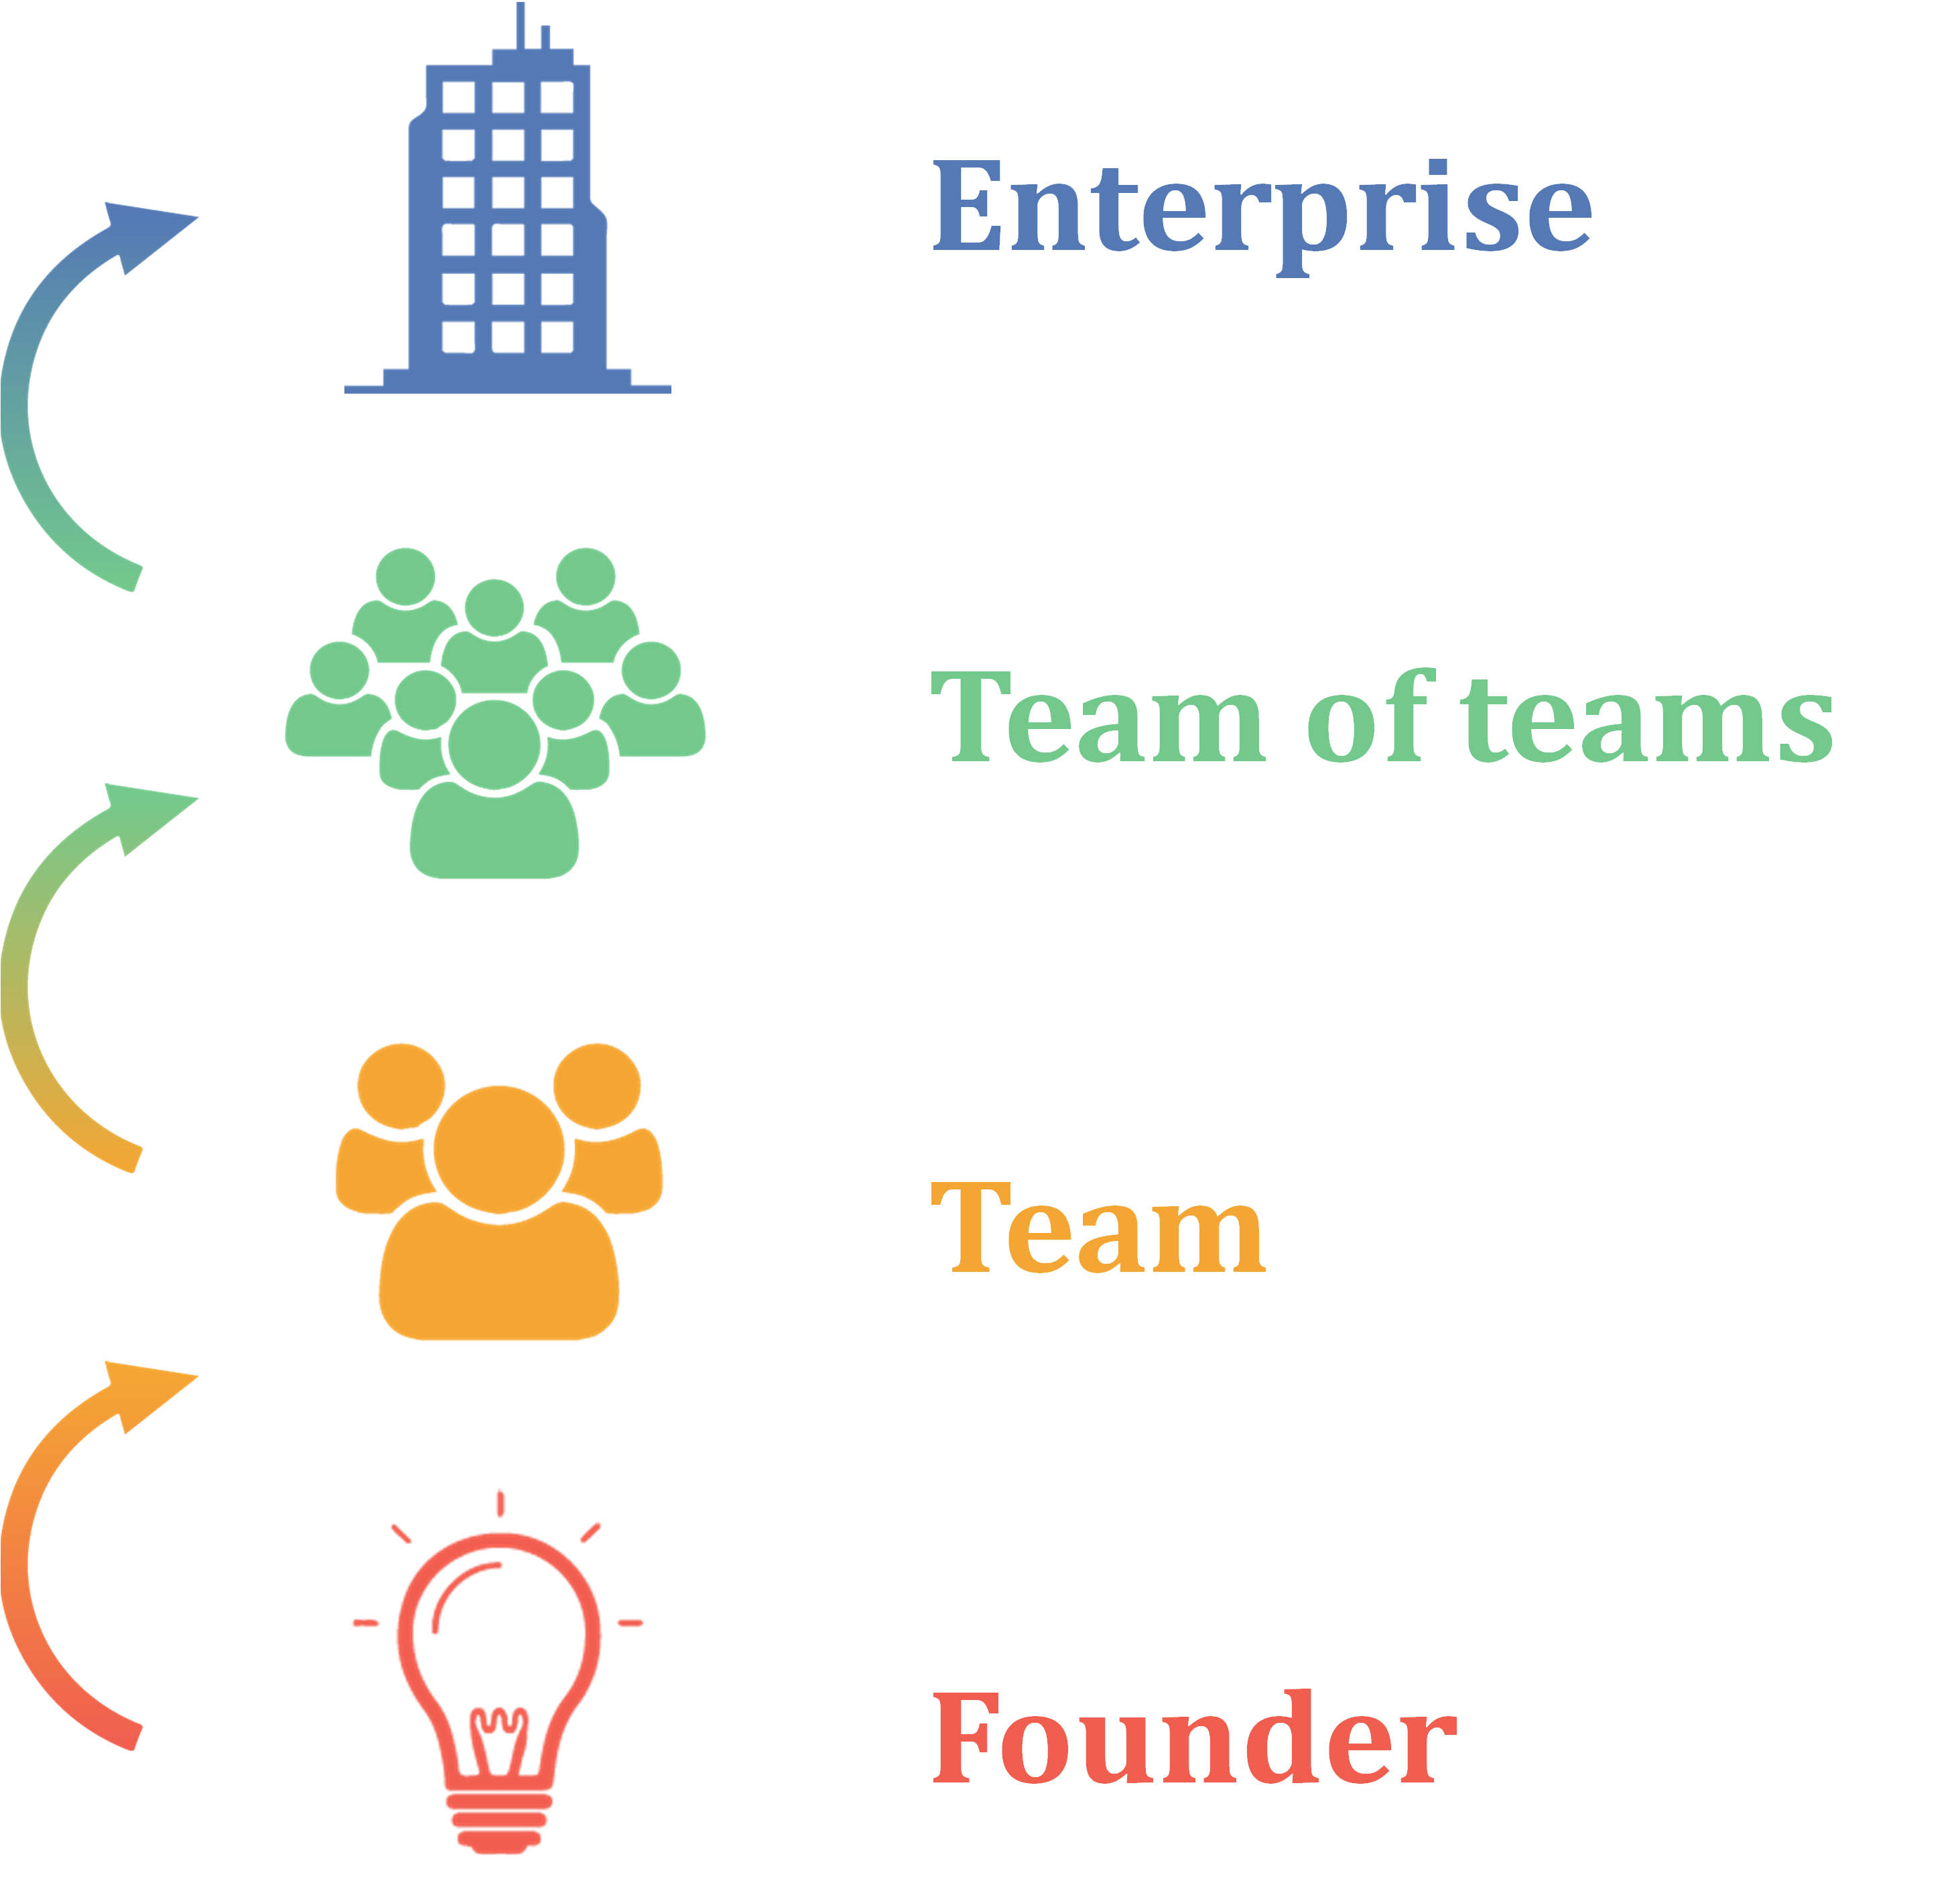
\includegraphics[width=0.48\textwidth]{images/emergence.png}}}}{emergence}
\end{center}
\caption{IT management evolutionary model (read bottom to top)}
\end{wrapfigure}
 
Elaborating the above outline into chapters, we have:
 \begin{enumerate}[label=\Roman*.]

\item{} \textbf{Founder}
 \begin{enumerate}[label=\arabic*.]

\item{} \textbf{IT value.} Why do we need computers? What can they do for us?
 

\item{} \textbf{IT infrastructure.} We want to build something. We have to choose a platform first.
 

\item{} \textbf{IT applications.} Let's start building something of use to someone.
 
\end{enumerate}
 

\item{} \textbf{Team}
 \begin{enumerate}[label=\arabic*.]

\item{} \textbf{Product management.} What exactly is it that we are building? What is the process of discovering our customer's needs and quickly testing how to meet them? How do we better define the product vision, and the way of working towards it, for a bigger team?
 

\item{} \textbf{Work management.} How do we keep track of what we are doing and communicate our progress and needs at the simplest level?
 

\item{} \textbf{Operations management.} How do we sustain this surprisingly fragile digital service in its ongoing delivery of value?
 
\end{enumerate}
 
\end{enumerate}
 
\textbf{The boundary between the \textquotedblleft{}team\textquotedblright{} and the \textquotedblleft{}team of teams\textquotedblright{} is a challenging area, and industry responses remain incomplete and evolving\textemdash{}hence the notation \textquotedblleft{}THE SCALING PROBLEM\textquotedblright{} on the diagram.}
 \begin{enumerate}[label=\Roman*.]

\item{} \textbf{Team of Teams}
 \begin{enumerate}[label=\arabic*.]

\item{} \textbf{Coordination.} When we have more than one team, they need to \emph{coordinate}, which we define as "the process of managing dependencies among activities." There are many synchronization techniques to help us coordinate, including project and process management and Agile concepts.
 

\item{} \textbf{Planning and investment.} We make investments in various products, programs, and/or projects, and we are now big enough that we have portfolios of them. How do we decide? How do we choose and work with our suppliers? How do we manage the finances of complex digital organizations?
 

\item{} \textbf{Organization and culture.} We're getting big. How do we deal with this? What are the unwritten values and norms in our company? How are we structured, and why that way? How can we benefit from increasing maturity and specialization while still maintaining a responsive digital product? How do we hire great people and get the most out of them?
 
\end{enumerate}
 

\item{} \textbf{Enterprise}
 \begin{enumerate}[label=\arabic*.]

\item{} \textbf{Governance, risk, security, and compliance.} We need to cope with structural and external forces (investors, directors, regulators, vendor partners, security adversaries, auditors) to whom we are ultimately accountable or who are otherwise defining our options. What are their motivations? How do we understand and control risk? How are we assured that our strategy, tactics, and operations are reasonable, sound, and thorough? And how do we protect ourselves from adversaries?
 

\item{} \textbf{Enterprise information management.} We've been concerned with data, information, and knowledge since the earliest days of our journey. But at this scale, we have to formalize our approaches and understandings; without that, we will never capture the full value available with modern analytics and big data. Compliance issues are also compelling us to formalize here.
 

\item{} \textbf{Architecture and portfolio.} We need to understand the big picture of interacting lifecycles, reduce technical debt and redundancy, accelerate development through establishing platforms, and obtain better economies of scale. We do so in part through applying techniques such as visualization, standardization, and portfolio management. We need to define our investment strategy based on a sound understanding of both business needs and technology limitations.
 
\end{enumerate}
 

\item{} \textbf{Appendices}
 \begin{enumerate}[label=\arabic*.]

\item{} \textbf{A review of IT frameworks and standards}
 

\item{} \textbf{Project management fundamentals}
 

\item{} \textbf{Process management fundaments}
 

\item{} \textbf{Towards a theory of IT management}
 

\item{} \textbf{Recommended readings}
 

\item{} \textbf{References}
 

\item{} \textbf{Glossary}
 

\item{} \textbf{Colophon}
 
\end{enumerate}
 
\end{enumerate}
 
\label{formalization}\hyperlabel{formalization}
  
\section{Emergence means formalization}
\label{_emergence_means_formalization}\hyperlabel{_emergence_means_formalization}%
  
The emergence model seeks to define a likely order in which concerns are \textbf{formalized}. Any concern may of course arise at any time\textemdash{}the startup founder certainly is concerned with security! Formalization means at least one or more of the following:
 \begin{itemize}

\item{} Dedicated resources
 

\item{} Dedicated organization
 

\item{} Defined policies and processes
 

\item{} Automated tooling
 
\end{itemize}
 
In the author's experience, for example, startups avoid formalized process and project management. To the extent the concerns exist, they are \emph{tacit} (understood or implied; suggested; implicit). Certainly, a small startup does not invest in an enterprise-{}class service desk tool supporting a full array of IT management processes or a full-{}blown project management office with its own vice president and associated portfolio automation. Simple work management, with a manual or automated Kanban board, is likely their choice for work management.
 
But by the time they are a team of teams, specialization has emerged and more robust processes and tools are required. Finally, the more complex, enterprise-{}scale concerns at the end of the book are presented as part of a logical progression.
 
The danger of course is that the formalization effort may be driven by its own logic and start to lose track of the all-{}critical business context. By carefully examining these stages of maturation, and the industry responses to them, it is the author's hope that the student will have effective tools to critically engage with the problem of scaling the digital organization.
  
% ------- 
% Chapter 
% ------- 

\chapter{Part I: Founder}
\label{Part-I-intro}\hyperlabel{Part-I-intro}%
  
\label{Sec-I}\hyperlabel{Sec-I} This is the introduction to part I.
 
In this section, we explore the fundamentals of information technology delivery.
 
\textbf{Scenario}
 
You are working in a startup, alone or with one or two partners. You are always in the same room, easily able to carry on a running conversation about your efforts and progress. You have no time or resources to spend on anything except keeping your new system alive and running.
 
\textbf{Chapter 1: IT Value}
 
Chapter 1 introduces you to the fundamental concepts of IT value that serve as a basis for the rest of the course. Why do people want computing (IT) services? What are the general outlines of their structure? How do they come into being? How are they changed over time?
 
All of this is essential to understand for your scenario; you need to understand what computers can do and how they are generally used if you are going to create a product based on them.
 
This chapter also covers the basics of how you'll approach building a product. It's assumed you won't develop an intricate, long-{}range plan but rather will be experimenting with various ideas and looking for fast feedback on their success or failure.
 
\textbf{Chapter 2: IT Infrastructure}
 
In this chapter, you have a general idea for a product and are ready to start building it. But not so fast\ldots{}\hspace{0em}you need to decide some fundamentals first. How will your new product run? What will you use to build it?
 
It's not possible to begin construction until you decide on your tools. This chapter will provide you an overview of computing infrastructure including cloud hosting and various approaches to system configuration.
 
This chapter also presents an overview of source control, as even your infrastructure depends on it in the new world of \textquotedblleft{}infrastructure as code.\textquotedblright{}
 
\textbf{Chapter 3: Application delivery}
 
Finally, you're ready to start building something. While this is not a book on software development or programming languages, it's important to understand some basics and at least see them in action.
 
This is also the \textquotedblleft{}DevOps\textquotedblright{} chapter; it's not just about writing code but about the entire end-{}to-{}end system that gets the code you are writing from your workstation, into collaborative environments, and finally to a state where it can be accessed by end users. From source repository to build manager to package repository to production, we'll cover a basic toolchain that will help you understand modern industrial practices.
 
\textbf{This section's lab approach}
 
While this is not a book about any particular computing language or platform, we need to describe some technical fundamentals. We'll do so in as neutral a manner as possible. However, this book's accompanying labs are based on \href{http://www.ubuntu.com/}{Ubuntu Linux} and \href{https://git-scm.com/}{git}, the distributed version control system created by Linus Torvalds to facilitate Linux development.
 \begin{DBKadmonition}{warning}{Important}
 
Part II, like the other parts, needs to be understood as a unified whole. In reality, digital entrepreneurs struggle with the issues in all three chapters simultaneously.
 \end{DBKadmonition}
 
\section{Chapter 1: IT Value}
\label{Intro-Chap-1}\hyperlabel{Intro-Chap-1}%
  
\subsection{Introduction}
\label{_introduction}\hyperlabel{_introduction}%
  
\emph{Collaboration notes}
 
\emph{I am concerned that the discussion of Carr \& related topics is a bit advanced for introductory students. Or perhaps the flow is off. Thoughts appreciated.}
 
\emph{-{}ctb}
 
As noted at the outset, you are a small core of a startup. You are building a product of which IT is a significant part. Your motivations are entrepreneurial; you want to create a successful business. You might be housed within a larger enterprise, but the thought experiment here is that you have substantial autonomy to order your efforts.
You want to do something that has a unique IT component. Regardless of your business, you will need accounting and legal services at a minimum and, very quickly, payroll and HR and so forth. Those things can (and should) be purchased as commodity services if you are a small entrepreneur (I am not aware of any convincing arguments to the contrary, unless you are absolutely on the smallest of shoestring budgets and can work 100-{}hour weeks). Your unique value proposition will be expressed to some degree in unique IT software. While this software may be based on well-{}understood products, the configuration and logic you construct will be all your own. Because of this, you are now a producer (or soon to be) of IT services.
 
Before we can talk about building and managing information technology (IT), we need to understand what it is and why people want it. We'll start this chapter by looking at an IT value experience that may seem very familiar. Then we'll dig further into concepts like the IT stack and the IT service and how they change over time.
 
\subsubsection{Chapter outline}
\label{_chapter_outline}\hyperlabel{_chapter_outline}%
  \begin{itemize}

\item{} An IT value experience
 

\item{} What is information technology?
 

\item{} The IT \emph{service} and the IT \emph{stack}
 

\item{} The IT service
 

\item{} IT changing over time
 

\item{} The digital context
 

\item{} Conclusion
 
\end{itemize}
  
\subsubsection{Learning objectives for this chapter}
\label{_learning_objectives_for_this_chapter}\hyperlabel{_learning_objectives_for_this_chapter}%
  \begin{itemize}

\item{} Explain \textquotedblleft{}IT value\textquotedblright{} in everyday terms
 

\item{} Distinguish between IT service and IT system
 

\item{} Discuss how IT services change over time
 

\item{} Describe various ways of understanding the context in which digital systems are developed and digital value is delivered.
 
\end{itemize}
   
\subsection{What is IT value?}
\label{_what_is_it_value}\hyperlabel{_what_is_it_value}%
  
\label{what-is-IT-value}\hyperlabel{what-is-IT-value}
 
\subsubsection{An IT value scenario}
\label{_an_it_value_scenario}\hyperlabel{_an_it_value_scenario}%
  \begin{wrapfigure}{r}{0.5\textwidth}[H]

\begin{center}
\imgexists{images/1_01c-women.png}{{\imgevalsize{images/1_01c-women.png}{
\includegraphics[width=0.48\textwidth]{images/1_01c-women.png}}}}{women w/cell phones}
\end{center}
\caption[{Dinner out tonight? }]{Dinner out tonight? \footnotemark{}}
\label{women.png-450-r}\hyperlabel{women.png-450-r}%
\end{wrapfigure}
 
Consider the following scenario:
 
A woman is wondering if she can afford to dine out that evening.\footnote{
\emph{Image credit \href{https://www.flickr.com/photos/garryknight/700317885/}{https://www.flickr.com/\-photos/\-garryknight/\-700317885/\-}, downloaded 2016-{}09-{}14, commercial use permitted}
}
 \begin{itemize}

\item{} She uses her mobile device to access her banking information and determines that in fact she does have enough money to do so.
 

\item{} She also uses her mobile device to make a reservation and contact some friends to join her.
 

\item{} Finally, she uses social navigation software to avoid heavy traffic, arriving at the restaurant in time for an enjoyable evening with her friends.
 
\end{itemize}
 
Information technology pervaded this experience. The origins, layers, and complex connections of the distributed systems involved are awe-{}inspiring to consider.
 \begin{DBKadmonition}{warning}{Important}
 
\textbf{Don't worry about the technological terms for now.}  This is an introductory text. You may see terms below that are unfamiliar (model-{}view-{}controller, IP, packet switching). If you are reading this online, you can follow the links, but it's not required. As you progress in your career, you will always be encountering new terminology. Part of what you need to learn is when it's important to dig into it and when you can let it pass for a time. You should be able to understand the gist presented below that these are complex systems based on a wide variety of technologies, some of them old, some new.
 \end{DBKadmonition}
 
The screen on her cell phone represents information accessed and presented via a \href{https://en.wikipedia.org/wiki/Model%E2%80%93view%E2%80%93controller}{model-{}view-{}controller framework}, implemented in the latest version of \href{https://developer.mozilla.org/en-US/docs/Web/JavaScript}{JavaScript}, running on an \href{https://en.wikipedia.org/wiki/Interpreter_(computing)}{interpreter} that would have taxed a \href{https://en.wikipedia.org/wiki/Mainframe_computer}{mainframe} thirty years ago. The communication with her bank's central systems is supported by \href{https://en.wikipedia.org/wiki/LTE_(telecommunication)}{4G LTE} data which in turn relies on the high-{}volume \href{https://en.wikipedia.org/wiki/Internet_Protocol}{IP backbone} networks operated by the \href{http://searchnetworking.techtarget.com/definition/telecom-carrier}{telecommunications carriers}, based on research into \href{https://en.wikipedia.org/wiki/Packet_switching}{packet switching} now approaching fifty years old.
The application operating on the cell phone interacts with core banking systems via sophisticated and highly secure \href{https://en.wikipedia.org/wiki/Middleware}{middleware}, crossing multiple \href{https://en.wikipedia.org/wiki/Computer_network}{network} control points. This middleware talks in turn to the customer demand deposit system that still runs on the mainframe.
 
The mainframe is now running the latest version of \href{https://en.wikipedia.org/wiki/Z/OS}{IBM's z/\-OS} \href{https://en.wikipedia.org/wiki/Operating_system}{operating system} (a direct descendant of \href{https://en.wikipedia.org/wiki/OS/360_and_successors#MVT}{OS/\-360}, one of the most significant operating systems in the \href{https://en.wikipedia.org/wiki/History_of_computing}{history of computing}). The customer demand deposit banking application running on the mainframe is still based on code written in the lowest level \href{https://en.wikipedia.org/wiki/Assembly_language}{assembler}. Some of the comments in this code date back to the 1970s. It has been tuned and optimized over the decades into a system of remarkable speed and efficiency. Although replatforming it is periodically discussed, the cost/benefit ratio for such a project has to date not been favorable.
 
The reservation system looks similar on the mobile device, but the network routes it to a large \href{https://en.wikipedia.org/wiki/Cloud_computing}{cloud} data center hosting the reservation system. The back end application here is very different from the banking system; the \href{https://en.wikipedia.org/wiki/Programming_language}{programming languages} are newer, the \href{https://en.wikipedia.org/wiki/Database}{database} is structured very differently, and the operating system is \href{https://www.linux.com/}{Linux}.
 
Finally, the navigation software looks much like the reservation system, as it too is based on the cloud. However, the system is much more active as it is continually processing inputs from millions of drivers in thousands of cities and updating traffic maps for those drivers in real time so that they can choose the most optimal route to their destinations (e.g., dinner). The capabilities of this system are comparable to an air traffic control system, and yet it is available as a free download for our IT user.
 \begin{wrapfigure}{r}{0.5\textwidth}[H]

\begin{center}
\imgexists{images/1_01-friends.jpg}{{\imgevalsize{images/1_01-friends.jpg}{
\includegraphics[width=0.48\textwidth]{images/1_01-friends.jpg}}}}{party}
\end{center}
\caption[{Digital made this gathering easier }]{Digital made this gathering easier \footnotemark{}}
\end{wrapfigure}
 
The resulting value is clear:
 \begin{itemize}

\item{} In an earlier era, our user might have stayed in for fear of bouncing a check, or she might have gone out and dined beyond her means.
 

\item{} The phone line at the restaurant might have been busy, so she might have risked showing up with no reservation.
 

\item{} Before texting and social media, she might not have been able to reach her friends as easily.
 

\item{} Without the traffic application, she might have run into a huge midtown traffic jam and been half an hour late.
 
\end{itemize}
 
Clearly, information technology added value to her life and helped maximize her experience of social enjoyment.
  
\subsubsection{Various forms of IT value}
\label{_various_forms_of_it_value}\hyperlabel{_various_forms_of_it_value}%
  
As we have seen, there are many ways in which digital systems deliver value. Some systems serve as the modern equivalent of file cabinets: massive and secure storage for financial transactions, insurance records, medical records, and the like. Other systems enable the transmission of information around the globe, whether as emails, web pages, voice calls, video on demand, or data to be displayed in a smartphone application (app). Some of these systems support engaged online communities and social interactions with conversations, media sharing, and even massive online gaming ecosystems. Yet other systems enable penetrating analysis and insight by examining the volumes of data contained in the first two kinds of systems for patterns and trends. Sophisticated statistical techniques and cutting-{}edge approaches like neural network-{}based machine learning increase the insights our digital systems are capable of, at a seemingly exponential rate.
 
Digital technology generates value in both direct and indirect ways. People have long consumed (and paid for) communication services, such as telephone services. Broadcast entertainment was a different proposition, however. The consumer (the person with the radio or television) was not the customer (the person paying for the programming to go out over the airwaves). New business models sprung up to support the new media through the sale of advertising air time. In other words, the value proposition was indirect, or at least took multiple parties to achieve: the listener, the broadcaster, and the advertiser. Finally, some of the best known uses of digital technology were and are very indirect\hspace{0.167em}\textemdash{}\hspace{0.167em}the above-{}mentioned banks and insurance agencies using the earliest computers to automate the work of thousands of typists and file clerks.
From these early business models have evolved and blossomed myriads of creative applications of digital technology for the benefit of human beings in their ongoing pursuit of happiness and security. We see the applications mentioned at the outset: online banking, messaging, restaurant reservation, and traffic systems. Beyond that we see the use of digital technology in nearly every aspect of life. (And I say \textquotedblleft{}nearly\textquotedblright{} only because I am a cautious person.)
 
Digital and information technology pervades all of the major industry verticals (e.g., manufacturing, agriculture, finance, retail, healthcare, transportation, services) and common industry functions (e.g., supply chain, human resources, corporate finance, and even IT itself).
 
Digital systems and technologies also are critical components of larger scale industrial, military, and aerospace systems. For better or worse, general purpose computers are increasingly found controlling safety-{}critical infrastructure and serving as an intermediating layer between human actions and machine response. Robotic systems are based on software, and the Internet of Things ultimately will span billions of sensors and controllers in interconnected webs monitoring and adjusting all forms of complex operations across the planet.
   
\subsection{Defining Information Technology}
\label{_defining_information_technology}\hyperlabel{_defining_information_technology}%
  
\label{what-is-IT}\hyperlabel{what-is-IT}
 
\subsubsection{What is IT, anyways?}
\label{_what_is_it_anyways}\hyperlabel{_what_is_it_anyways}%
  
We've started this book in the previous section by providing an example of digital or IT value, without much discussion of how it is delivered. This is deliberate. But what is IT (Information Technology), anyways?
 \begin{itemize}

\item{} The computers? The networks?
 

\item{} The people who run them?
 

\item{} That organization under a Chief Information Officer that loves to say \textquotedblleft{}no\textquotedblright{} and is always slow and expensive?
 
\end{itemize}
 
None of these are how this book defines \textquotedblleft{}IT.\textquotedblright{} Although this is not a technical book on computer science or software engineering, the intent is that it reflects and is compatible with foundational principles.
 
\textquotedblleft{}Information technology\textquotedblright{} is ultimately based on the work of \href{https://en.wikipedia.org/wiki/Claude_Shannon}{Claude Shannon}, \href{https://en.wikipedia.org/wiki/Alan_Turing}{Alan Turing}, \href{https://en.wikipedia.org/wiki/Alonzo_Church}{Alonzo Church}, \href{https://en.wikipedia.org/wiki/John_von_Neumann}{John von Neumann}, and the other pioneers who defined the central problems of \href{https://en.wikipedia.org/wiki/Information_theory}{information theory}, \href{https://en.wikipedia.org/wiki/Digital_electronics}{digital logic},  \href{https://en.wikipedia.org/wiki/Computability}{computability}, and \href{https://en.wikipedia.org/wiki/Computer_architecture}{computer architecture}.
 
\label{IT-as-function}\hyperlabel{IT-as-function}
 
Additionally, as an organizational function, information technology also draws on organizational theory, systems theory, human factors and psychology, and more recent concepts such as design thinking, among many other areas.
 
Discussions of \textquotedblleft{}information technology\textquotedblright{} become contentious because some think of the traditional organization, while others think of the general problem area. IT has a long history as a corporate function, a single hierarchy under a powerful Chief Information Officer. This model has had its dysfunctions, including a longstanding reputation for being slow and expensive. Often, when one encounters the term \textquotedblleft{}IT,\textquotedblright{} the author using the term is referring to this organizational tradition.
 
\textbf{We are less interested in the future of IT as a distinct organizational structure. There are many different models, from fully centralized to fully embedded.} Organizational structure will be discussed in Chapter 7.
 
For this book, we define \textquotedblleft{}Information technology\textquotedblright{} in terms of its historic origins. We look to IT's common origins in automating the laborious and error prone processes of computation, through the application of digital logic technologies based on information transmission.
 
Regardless of organizational form or delivery methods, IT is defined by these origins. And there are notable common threads throughout this problem domain: the fragility and complexity of these systems, the need for layered abstractions in their management, and more.
 
It does not matter if the application developers ultimately report up through the CIO, the CMO, the CFO, or the COO. Their daily experience remains largely the same. The dynamics of their management remain the same. Executives who seek to take control of IT so they can \textquotedblleft{}remove that old bureaucracy\textquotedblright{} are well advised to be cautious; the bureaucracy emerged for a reason. More on this in subsequent chapters.
 
\label{digital-transformation}\hyperlabel{digital-transformation}
  
\subsubsection{IT and digital transformation}
\label{_it_and_digital_transformation}\hyperlabel{_it_and_digital_transformation}%
  \begin{quote}

IT doesn't matter.

\hspace*\fill--- Nicholas Carr
\end{quote}
 \begin{quote}

Software is eating the world.

\hspace*\fill--- Mark Andreessen
\end{quote}
 \begin{quote}

The digital realm is infusing the physical realm, like tea in hot water.

\hspace*\fill--- Jeff Sussna
\emph{Designing Delivery} \end{quote}
 
IT increasingly permeates business operations and social interactions. The breadth and depth of IT support for virtually all domains of society continues to expand. Lately, this is known as digital transformation.
 
The role of information technology seems critical to society and the economy, but there are various points of view. Nicholas Carr, in his controversial \emph{Harvard Business Review} article "IT Doesn't Matter," recognized that IT was becoming commoditized in an important sense \hyperlink{Carr2003}{[Carr2003]}. As Cloud providers started to offer utility-{}style computing, the choice of particular vendors of computers was no longer strategic. Looking to history, Carr argued that just as businesses no longer have \textquotedblleft{}Vice Presidents for Electricity,\textquotedblright{} so businesses no longer need Chief Information Officers or dedicated IT departments.
 \begin{DBKadmonition}{}{Note}
 
A "commodity" product is one that is offered from a variety of suppliers, with little or no difference between their offerings. Commodity products tend to compete on price, not on differences in features. Wheat is a commodity. Sports cars are not. "Commoditization" is the process by which products that used to compete by being different, increasingly compete on price.
 \end{DBKadmonition}
 
Carr has insight\hspace{0.167em}\textemdash{}\hspace{0.167em}there is no question IT is becoming pervasive\hspace{0.167em}\textemdash{}\hspace{0.167em}but he ultimately reflects a narrow view of what \textquotedblleft{}IT\textquotedblright{} is. If \textquotedblleft{}IT\textquotedblright{} were merely computation at the lowest level\hspace{0.167em}\textemdash{}\hspace{0.167em}just shuffling bits of information around, doing a little math\hspace{0.167em}\textemdash{}\hspace{0.167em}then perhaps it could be embedded throughout a business like electricity.
 
But IT has emergent aspects that are not comparable to electrical power. As it pervades all dimensions of business operations, it brings its concerns with it: complexity, fragility, and the skills required to cope with them.
 
One watt of electrical power is like any other watt of electrical power, and can usefully be seen as a commodity. We can use it to run toasters, hair dryers, or industrial paint mixers, and there is little concern (beyond supply and demand management) that the consumption of power by the paint mixer will affect the toaster.  It's also true that one cycle of computing, in a certain sense, is like any other cycle. But information technology systems interact with each other in surprising and unpredictable ways, orders of magnitude more complex than electrical power grids. (This is not to imply the modern electrical grid is a simple system!)
 
IT also radically transforms industries: from retail to transportation to manufacturing to genetics. Applied software-{}centric IT is unleashing remarkable economic disruption.
 
A lawyer may depend on a cell phone, and (in keeping with Carr) beyond its provision as a commodity service, needs little else to deliver the legal strategies a firm needs. A graphic designer may use computerized graphic tools, but these have become relatively standardized and commoditized in the past twenty years, and probably are not a source of competitive advantage in the quest for new marketing clients.
 
On the other hand, consider a text analytic algorithm that replaces thousands of paralegals, resulting in order-{}of-{}magnitude more accurate legal research in a fraction of cost and time. This \textbf{is} strategic and disruptive to the legal community. A superior supply chain algorithm, and the ability to improve it on an ongoing basis, may indeed elevate a logistics firm's performance above competitors. In cases like these\hspace{0.167em}\textemdash{}\hspace{0.167em}and they seem to be increasing\hspace{0.167em}\textemdash{}\hspace{0.167em}IT matters very much. The annual State of DevOps research finds that "Firms with high-{}performing IT organizations were twice as likely to exceed their profitability, market share, and productivity goals." \hyperlink{Puppet2014}{[Puppet2014]}
 
In the digitally transforming economy, traditional \textquotedblleft{}back office\textquotedblright{} IT organizations find themselves called on to envision, develop, and support market-{}facing applications of IT. And what starts with one market-{}facing use case can quickly expand into entire portfolios.  It is such cases that are of particular concern in this book. Ultimately, it is possible that IT is the \textbf{most} strategic capability an organization can invest in. As the editor in chief of \emph{IEEE Software} notes \hyperlink{Spinellis2015}{[Spinellis2015]},
 \begin{quote}

other industries are also producing what's in effect software (executable knowledge) but not treating it as such . . . Although many industries have developed their own highly effective processes over the years, software engineering maintains an essential advantage. It has developed methods and tools that let even small teams manage extremely high complexity . . . This advantage is important because the complexity in non-{}software activities is also increasing inexorably . . . [T]he time has come to transform our world\ldots{} by giving back to science and technology the knowledge software engineering has produced.

\hspace*\fill--- Diomidis Spinellis
\emph{IEEE Software} \end{quote}
 
This ability to manage complexity, to turn tacit into explicit and formalize the previously unstructured, is an essential aspect of digital transformation.
  
\subsubsection{Defining "IT"}
\label{_defining_it}\hyperlabel{_defining_it}%
  
So, how do we define an IT problem, as opposed to other kinds of business problems? An IT problem is any problem where you are primarily constrained by your capability and understanding of IT.
 \begin{itemize}

\item{} If you need computer scientists or engineers who understand the fundamentals of information theory and computer science, you are doing IT.
 

\item{} If you need people who understand when your information-{}centric problems might need to be referred to such theorists and engineers, you are likely doing IT.
 

\item{} If you need people who are skilled in building upon those fundamentals, and operating technical platforms derived from them (such as programming languages, general purpose computers, and network routers), you are doing IT.
 
\end{itemize}
 
Regardless of whether IT is housed under a traditional CIO, an operations capability, a Chief Marketing Officer, or a \textquotedblleft{}line of business\textquotedblright{}, when it is critical to operations certain concerns inevitably follow:
 \begin{itemize}

\item{} Requirements (i.e. your intent for IT)
 

\item{} Sourcing and provisioning
 

\item{} IT-{}centric product design and construction
 

\item{} Configuration and change management
 

\item{} Support
 

\item{} Improvement
 
\end{itemize}
 
Executives who take control of information technology in hopes of making it more "agile" are often surprised to find that these concerns were not mere bureaucracy, but instead had well grounded origins in past failures. Ignoring these lessons is perilous.
 
And yet, the traditional, process-{}heavy IT organization does seem dysfunctional from a business point of view: a central theme of this book.
   
\subsection{IT services, systems, and applications}
\label{_it_services_systems_and_applications}\hyperlabel{_it_services_systems_and_applications}%
  
\subsubsection{Inside an IT service}
\label{_inside_an_it_service}\hyperlabel{_inside_an_it_service}%
  \begin{wrapfigure}{r}{0.5\textwidth}[H]

\begin{center}
\imgexists{images/1_01-ITValue.png}{{\imgevalsize{images/1_01-ITValue.png}{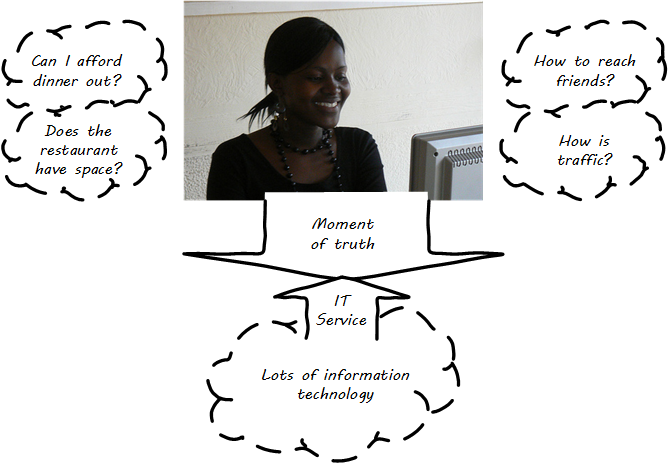
\includegraphics[width=0.48\textwidth]{images/1_01-ITValue.png}}}}{woman at computer}
\end{center}
\caption[{The basis of IT value }]{The basis of IT value \footnotemark{}}
\end{wrapfigure}
 
Let's examine our diner's value experience in more detail, without getting unnecessarily technical, and clarify some definitions along the way.  The first idea we need to cover is the "moment of truth." In terms of information technnology, this English-{}language clich� represents the user's experience of value.
 
Not sure that "moment of truth" is quite appropriate -{} original definition could be interpreted as something relatively infrequent in the customer journey\ldots{}\hspace{0em} perhaps "experience?"
 
In the example, our friend seeking a relaxing night out had several moments of truth:
 \begin{itemize}

\item{} Consulting her bank balance, and subsequent financial transactions also reflecting what was stated to her
 

\item{} Making a reservation and having it honored on arrival at the restaurant
 

\item{} Arriving on time to the restaurant, courtesy of the traffic application
 

\item{} And most importantly, having a relaxed and refreshing time with her friends.
 
\end{itemize}
 
Each of these individual value experiences was co-{}created by our friend's desire for value, and the response of a set of IT resources.
 \begin{DBKadmonition}{warning}{Important}
 
The "moment of truth" represents the user's experience of value, from a product, good, or service.
 \end{DBKadmonition}
 
In order to view her balance, our user is probably using an application downloaded from a "store" of applications made available to her device. On her device, this "app" is part of an intricate set of components performing functions such as:
 \begin{itemize}

\item{} accepting "input" (user intent) through a screen or voice input
 

\item{} processing that input through software and acting on her desire to see her bank balance
 

\item{} connecting to the phone network
 

\item{} securely connecting over the phone network to the Internet and then to the bank
 

\item{} identifying the user to the bank's systems
 

\item{} requesting the necessary information (in this case, an account balance)
 

\item{} receiving that information and converting it to a form that can be represented on a screeen
 

\item{} finally, displaying the information on the screen
 
\end{itemize}
 
The application, or "app," downloaded to the phone plays a primary role, but is enabled by:
 \begin{itemize}

\item{} the phone's operating system and associated services
 

\item{} the phone's hardware
 

\item{} the telecommunications infrastructure (cell phone towers, long distance fiber optic cables, switching offices, and much more)
 
\end{itemize}
 
Of course, without the banking systems on the other end, there is no bank balance to transmit. These systems are similar, but on a much larger scale than our friend's device:
 \begin{itemize}

\item{} Internet and middleware services to receive the request from the international network
 

\item{} Application services to validate the user's identity and route the request to the appropriate handling service
 

\item{} Data services to store the user's banking information (account identity and transactions) along with millions of other customers
 

\item{} Many additional services to detect fraud and security attacks, report on utilization, identify any errors in the systems, and much more.
 

\item{} Physical data centers full of computers and associated hardware including massive power and cooling infrastructure, and protected by security systems and personnel.
 
\end{itemize}
 \begin{wrapfigure}{r}{0.5\textwidth}[H]

\begin{center}
\imgexists{images/1_01-ITStack.png}{{\imgevalsize{images/1_01-ITStack.png}{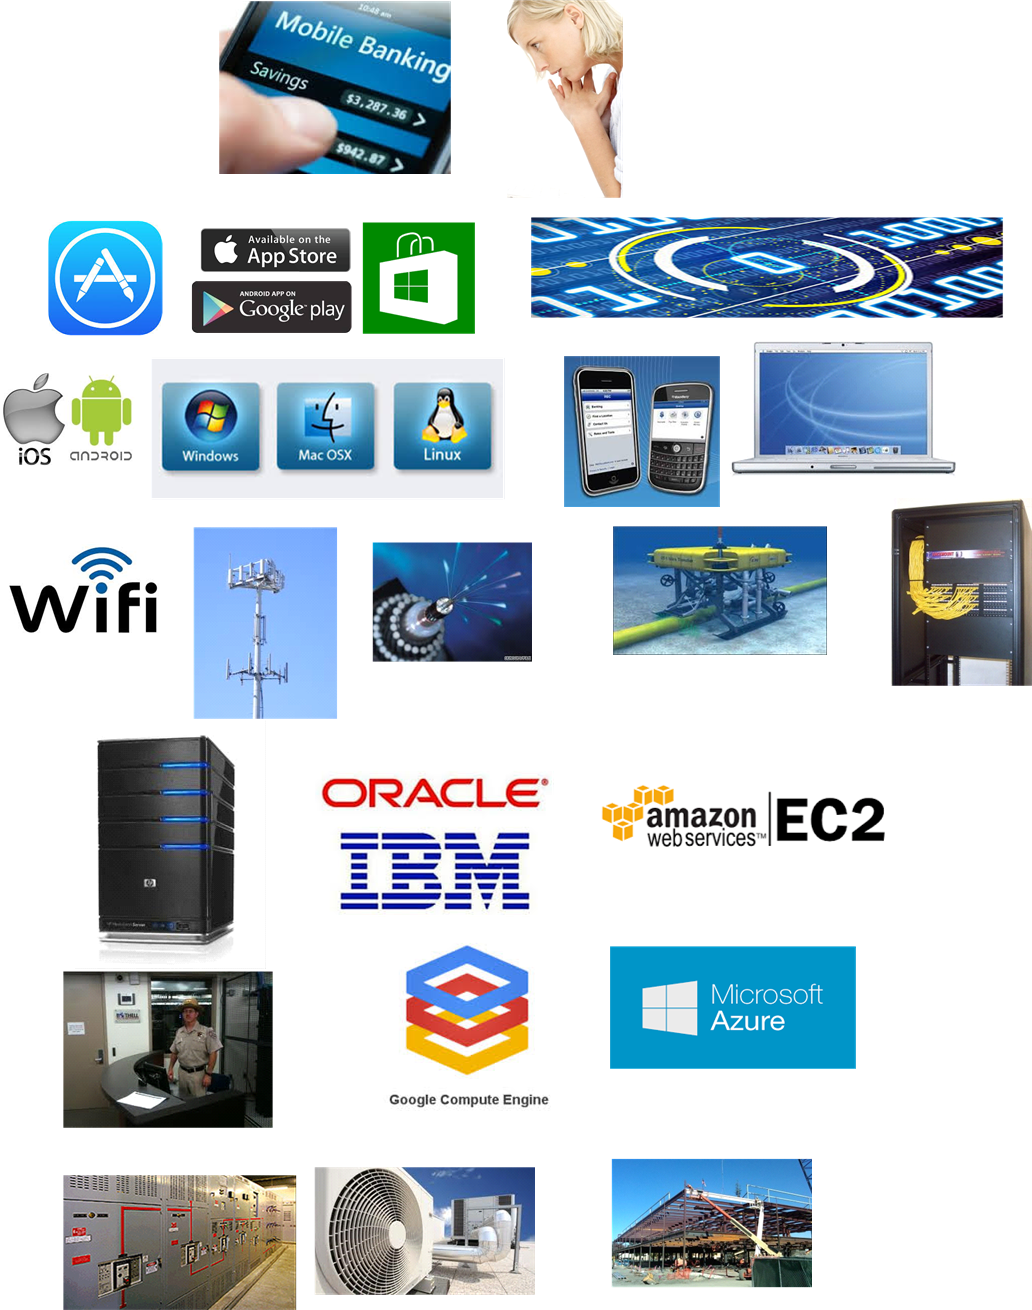
\includegraphics[width=0.48\textwidth]{images/1_01-ITStack.png}}}}{technologies}
\end{center}
\caption{The immensity of the IT stack}
\end{wrapfigure}
 
\begin{lstlisting}[firstnumber=1,backgroundcolor={},basicstyle=\ttfamily,]
#designer to provide concept guidance, and/or re-draw
\end{lstlisting}
 
Consider: what does all this mean to our user? Does she care about cell phone towers, or middleware, or triply-{}redundant industrial-{}strength Power Distribution Units? Usually, not in the least.
 
Therefore, as we study this world, we need to maintain awareness of her perspective. Our friend is seeking some value that IT uniquely can enable, but does not want to consider all the complexity that goes into it. She just wants to go out with friends. The moment of truth depends on the service; the service may contain great complexity, but part of its success lies in shielding the user from that complexity.
 \begin{wrapfigure}{r}{0.5\textwidth}[H]

\begin{center}
\imgexists{images/1_01-ITStack2.png}{{\imgevalsize{images/1_01-ITStack2.png}{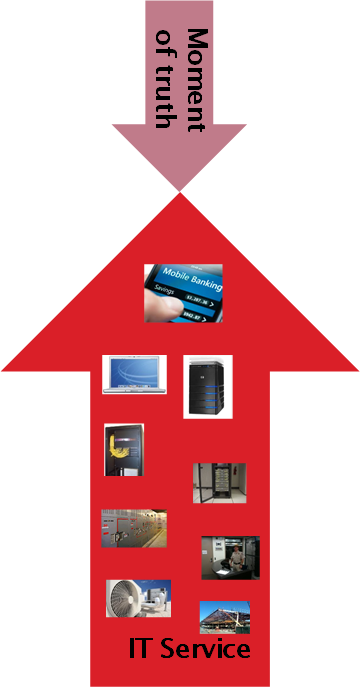
\includegraphics[width=0.48\textwidth]{images/1_01-ITStack2.png}}}}{ITStack}
\end{center}
\caption{The IT stack supports the moment of truth}
\end{wrapfigure}
 
\begin{lstlisting}[firstnumber=1,backgroundcolor={},basicstyle=\ttfamily,]
#designer to provide concept guidance, and/or re-draw
\end{lstlisting}
 \begin{DBKadmonition}{warning}{Important}
 
Always remember the user's experience. Information technology has a well deserved reputation for being too complicated for end users\textemdash{}\hspace{0em}for example, trying to do something that should be simple, and finding oneself in a technical conversation about network settings.
 \end{DBKadmonition}
  
\subsubsection{What versus how}
\label{_what_versus_how}\hyperlabel{_what_versus_how}%
  
This fundamental tension between \textbf{what} a system is supposed to do, versus \textbf{how} it does it, pervades IT management and will likely define your career. "Don't trouble me with the details, just give me the results" is the overall theme, and we encounter this reaction to complexity in many aspects of life.
 
Terminology is important. We need to have a more precise way of describing the information technology, beyond just saying there is "lots" of it. A variety of terms are used in this text:
 \begin{itemize}

\item{} IT service
 

\item{} Application
 

\item{} IT system
 

\item{} IT infrastructure
 
\end{itemize}
 
We also see discussion of components, resources, subsystems, assets, and many more terms.
 \begin{DBKadmonition}{warning}{Warning}
 
There are many debates around these definitions. Sometimes these debates are helpful in clarifying the terminology you want to use on your team. But sometimes the debates don't add any value. Beware of anyone who claims there is a "best practice" here.
 \end{DBKadmonition}
 
In general, in this book, we will use the following definitions:
 \begin{itemize}

\item{} An IT service is defined primarily in terms of WHAT not HOW
 

\item{} Defining an IT system may include a discussion of both WHAT it does and HOW it does it
 

\item{} An "application" usually means some IT service or system for end users who are not primarily concerned with IT other than wanting to get something done with it (e.g. go out to dinner)
 

\item{} "Infrastructure" usually means some IT service or system that primarily supports OTHER IT services or systems (e.g. a network "service" is not usually useful to end users without additional application services.)
 
\end{itemize}
 
Finally, the concept of the "IT stack" is important. Notice how the different technology layers appear "stacked." Layered approaches to understanding IT are common; see Further Reading for useful references.
 

\begin{sidebar}
\textbf{Author's note: Service versus product}


For the purposes of this book, "IT services" are equivalent to "products." You may in other contexts hear phrases like "products \textbf{versus} services" which imply that they are distinct. Usually, when products are contrasted with services, people are equating products with goods: a jar of peanut butter is a "product," while a haircut is a service.

However, when I worked at AT\&T, the internal term for offerings like broadband networking access was not "service," but "product." Services, in this sense, \textbf{are} products.

In this book, we see products and services as roughly equivalent, but the two terms have some different connotations. Products usually imply an external market, where services can be either internal or external facing. While we certainly talk about "product marketing", the term "service marketing" is rarely seen. Furthermore,  some organizations such as Target have recently re-{}conceptualized internal services organizations as "product teams."
\end{sidebar}
 
\label{service-lifecycle}\hyperlabel{service-lifecycle}
   
\subsection{The IT service lifecycle}
\label{_the_it_service_lifecycle}\hyperlabel{_the_it_service_lifecycle}%
  
We've established that the IT service is based on a complex stack of technology, from local devices to global networks to massive data centers. Software and hardware are layered together in endlessly inventive ways to solve problems people did not even know they had ten years ago.
 
But these IT service systems must come from somewhere. They must be designed, built, and operated, and (as any smartphone user can testify) they are continually improved over time.
 
A simple representation of the IT service lifecycle is shown in the figure below.
 \begin{enumerate}[label=\arabic*.]

\item{} It starts with an idea. Someone has an insight into an IT-{}enabled value proposition that can make a profit, or better fulfill a mission.
 

\item{} The idea must garner support and resources so that it can be built.
 

\item{} The idea is then constructed, at least as an initial proof of concept or Minimum Viable Product (in the language of Ries' \emph{Lean Startup}.) Construction is assumed to include an element of design; in this textbook, \textbf{construction and design are not represented as two separate phases.}
 

\item{} There is a critical state transition however that will always exist. Initially, it is the change from OFF to ON when the system is first constructed. After the system is ON, there are still distinct changes in state when new features are deployed, or incorrect behaviors ("bugs" or "defects") are rectified.
 

\item{} The system may be ON, but it is not delivering value until the user can access it. Sometimes, that may be as simple as providing someone with a network address, but usually there is some initial "provisioning" of system access to the user, who needs to identify themselves.
 

\item{} The system can then deliver services (moments of truth) to the end users. It may deliver millions or billions of such experiences, depending on its scale and how one might choose to count the subjective concept of value experience.
 

\item{} The user may have access, but may still not receive value, if they do not understand the system well enough to use it. Whether via a formal service desk, or informal social media channels, users of IT services will require and seek support on how to maximize the value they are receiving from the system.
 

\item{} Sometimes, support requests indicate that something is wrong with the system itself. If the system is no longer delivering value experiences (bank balances, restaurant reservations, traffic directions) then some action must be taken promptly to restore service.
 

\item{} All of the previous states in the lifecycle generate data and insight that lead to further evolution of the system. There is a wide variety of ways systems may evolve: new user functionality, more stable technology, increased system capacity, and more. Such motivations result in new construction and changes to the existing system, and so the cycle begins again.
 

\item{} \ldots{}\hspace{0em}Unless\ldots{}\hspace{0em} the system's time is at an end. If there is no reason for the system to exist any longer, it should be retired.
 
\end{enumerate}
 \begin{DBKadmonition}{}{Note}
 
System retirement is often more complex and expensive than expected, and there are many examples of systems surviving well beyond the point they deliver value.
 \end{DBKadmonition}
 \begin{wrapfigure}{r}{0.5\textwidth}[H]

\begin{center}
\imgexists{images/1_01-ITStates.png}{{\imgevalsize{images/1_01-ITStates.png}{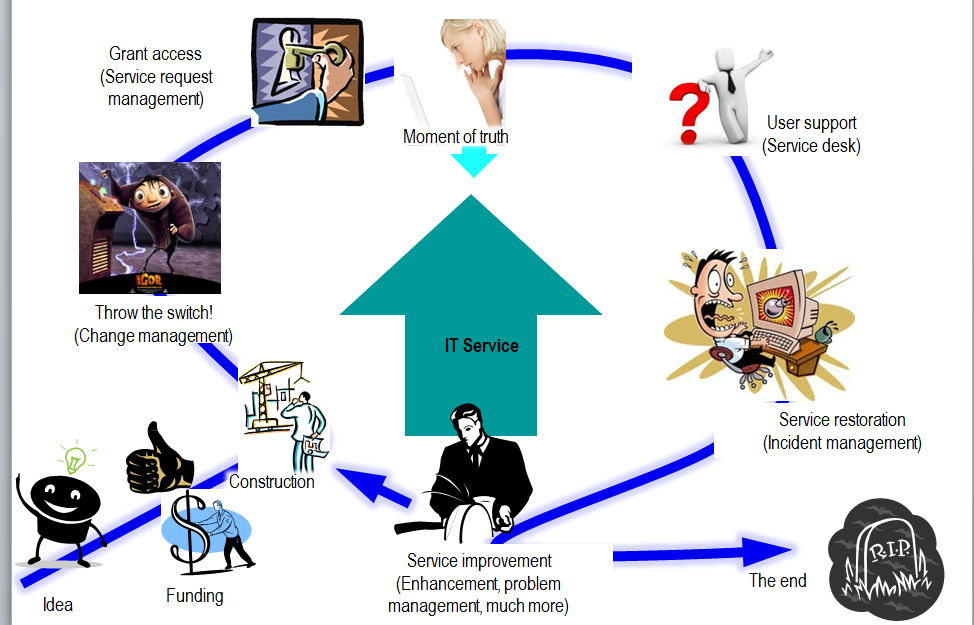
\includegraphics[width=0.48\textwidth]{images/1_01-ITStates.png}}}}{IT States}
\end{center}
\caption{The essential states of the digital service (or product)}
\end{wrapfigure}
 
So we see that the digital service/product evolves over time, through many repetitions ("iterations") of the improvement cycle. This entire process, from idea to decommissioning ("inspire to retire") can be understood as the \emph{service lifecycle}.
 \begin{wrapfigure}{r}{0.5\textwidth}[H]

\begin{center}
\imgexists{images/1_01-ITSvcChg.png}{{\imgevalsize{images/1_01-ITSvcChg.png}{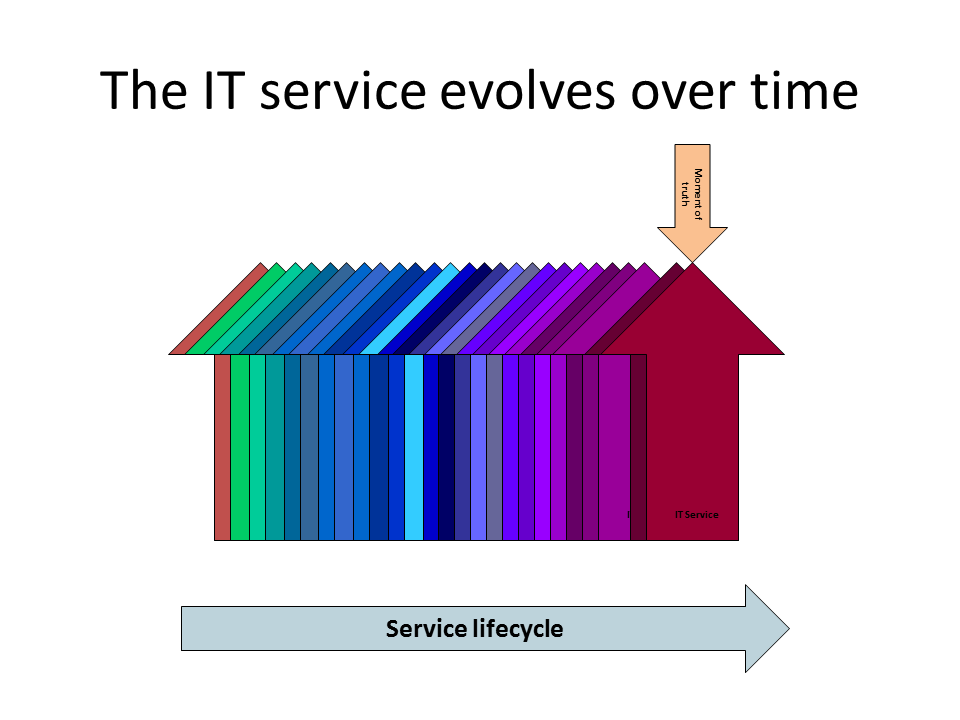
\includegraphics[width=0.48\textwidth]{images/1_01-ITSvcChg.png}}}}{IT service changes}
\end{center}
\caption{The IT service lifecycle}
\end{wrapfigure}
 
\begin{lstlisting}[firstnumber=1,backgroundcolor={},basicstyle=\ttfamily,]
#designer to provide concept guidance, and/or re-draw
\end{lstlisting}
 
\label{dual-axis-vc}\hyperlabel{dual-axis-vc}
 
We can combine the service experience (moment of truth) with the service/product lifecycle into the "dual-{}axis value chain" (originally presented in \hyperlink{Betz2011a}{[Betz2011a]}):
 \begin{wrapfigure}{r}{0.5\textwidth}[H]

\begin{center}
\imgexists{images/1_01-2-axis-value-chain.png}{{\imgevalsize{images/1_01-2-axis-value-chain.png}{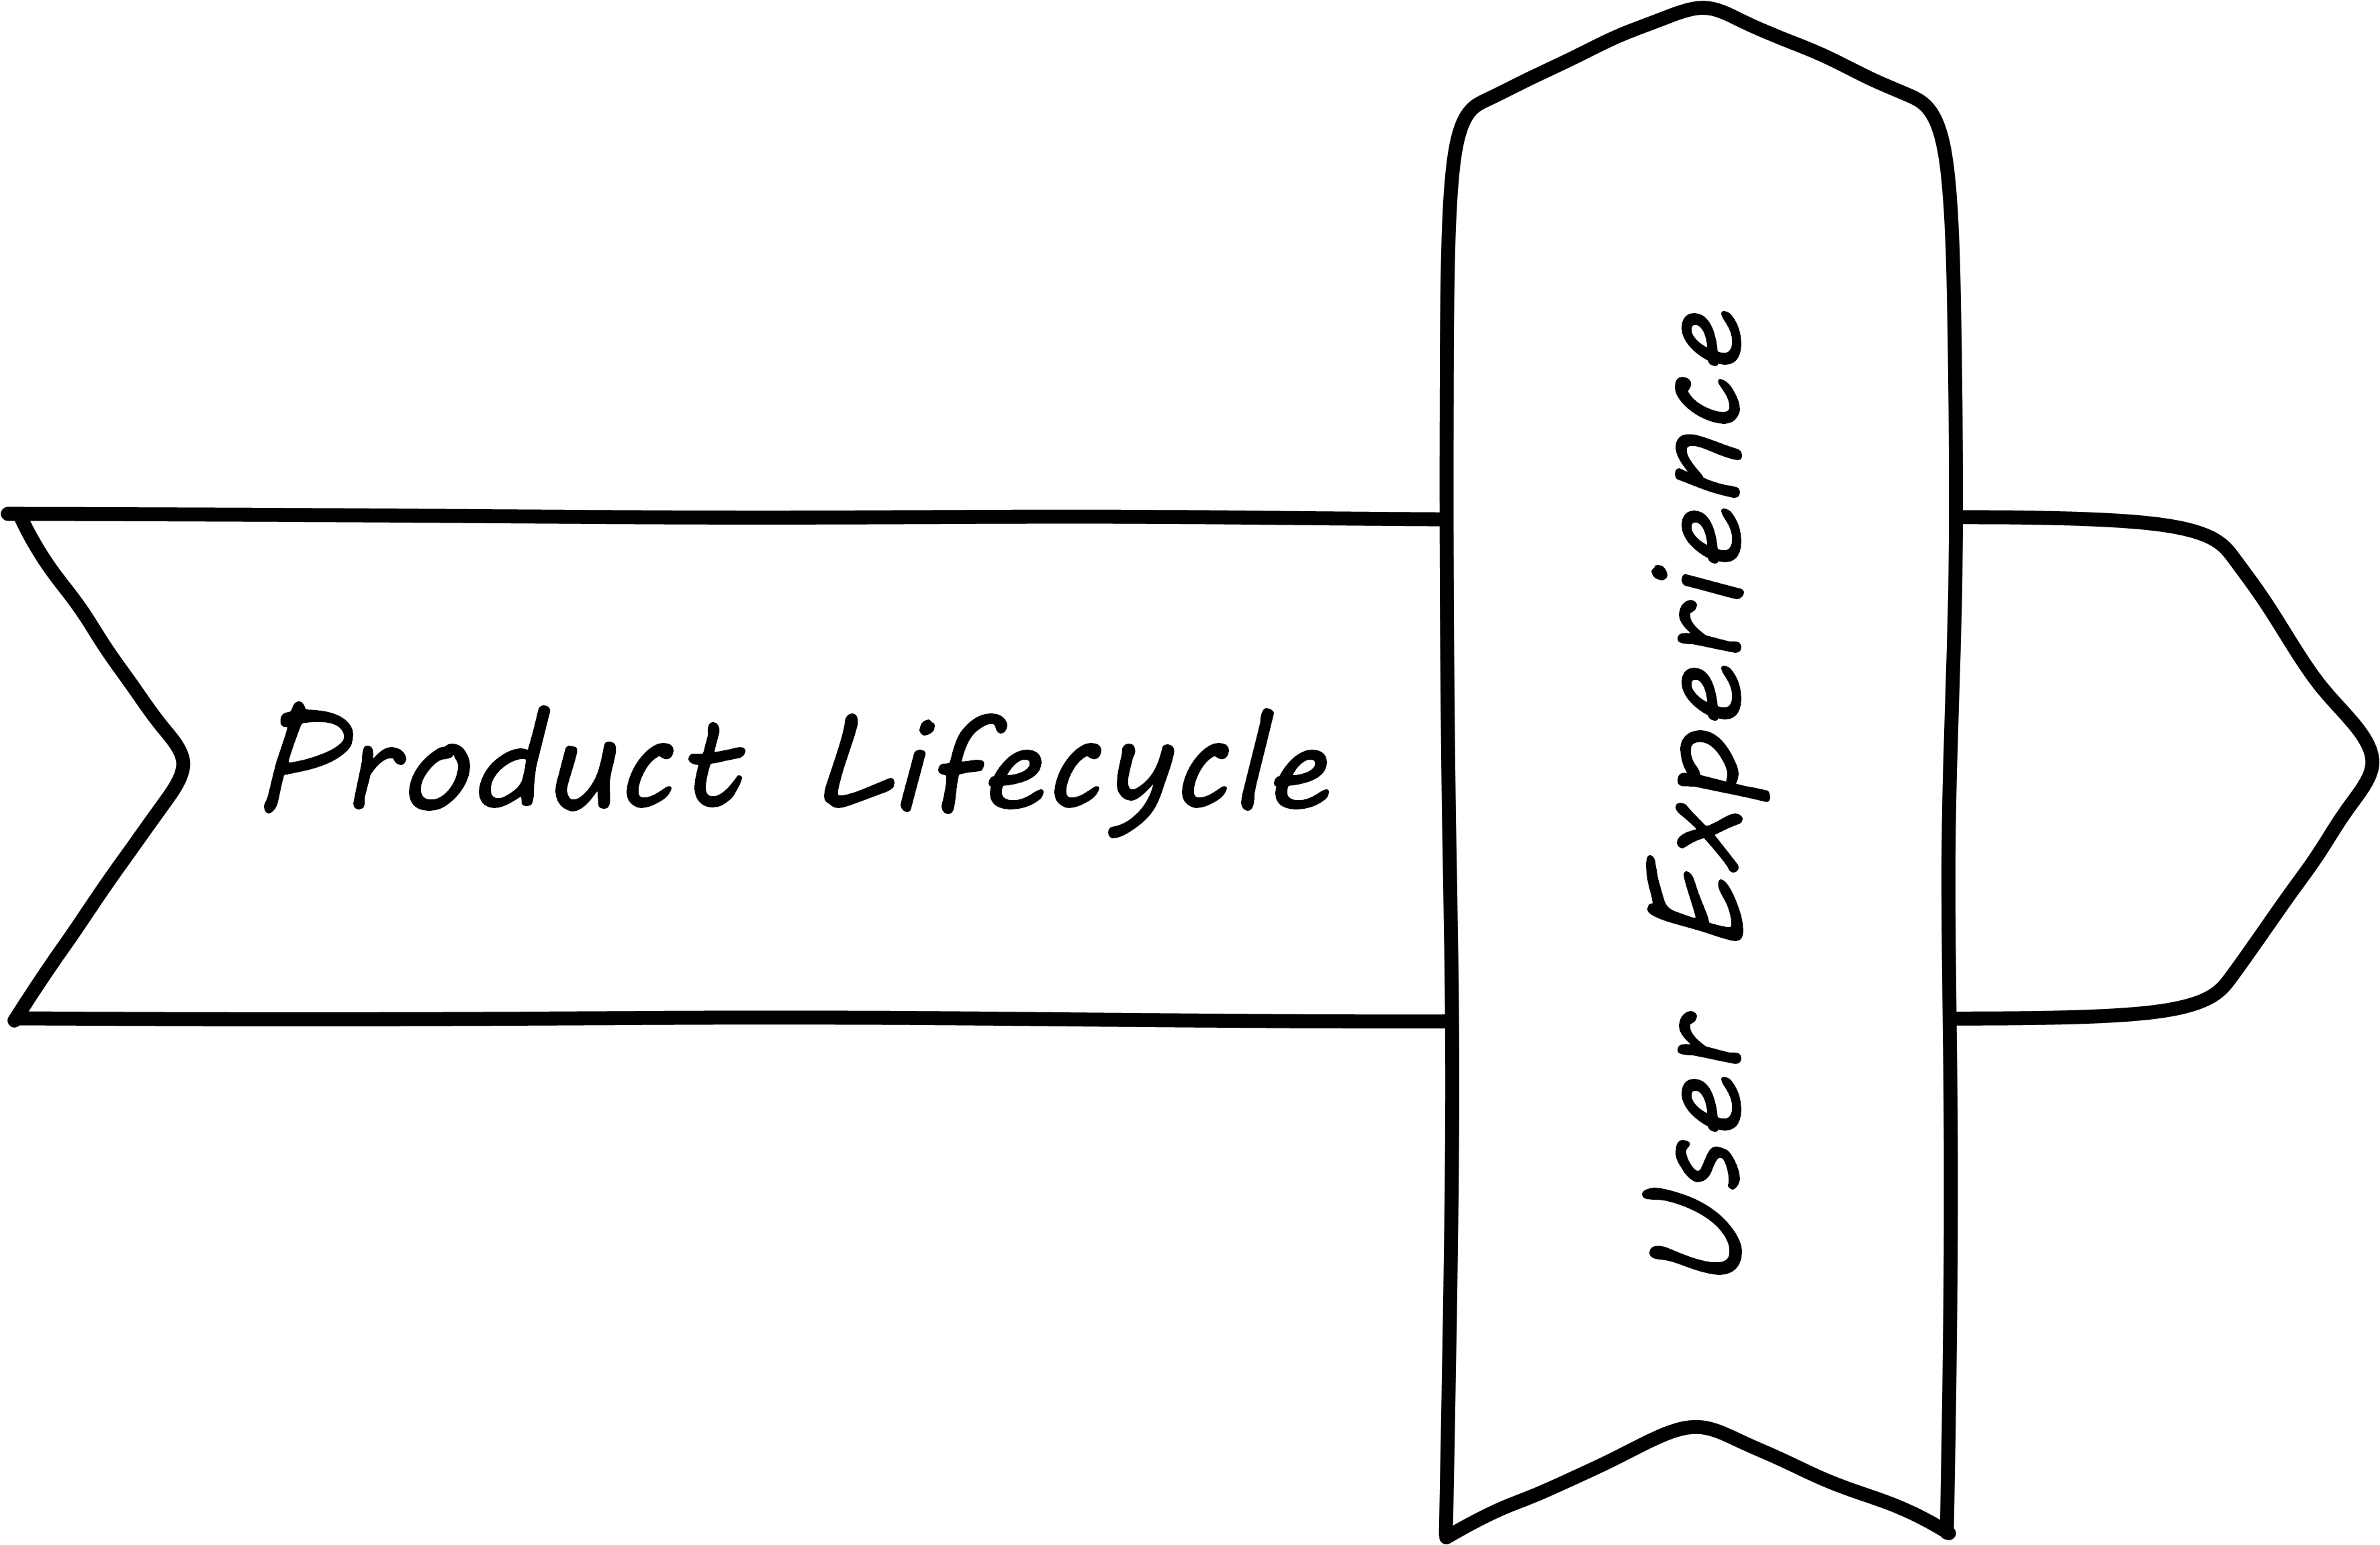
\includegraphics[width=0.48\textwidth]{images/1_01-2-axis-value-chain.png}}}}{2 axis value chain}
\end{center}
\caption{Dual-{}axis value chain}
\end{wrapfigure}
 
The 2-{}axis value chain can be seen in many representations of IT and digital delivery systems. Product evolution flows from right to left, while day to day value flows up, through the technical stack. It provides a basis for (among other things) thinking about the IT user, customer, and sponsor, which will cover in the next section.
 
\label{consumer-customer-sponsor}\hyperlabel{consumer-customer-sponsor}
  
\subsection{Defining consumer, customer, and sponsor}
\label{_defining_consumer_customer_and_sponsor}\hyperlabel{_defining_consumer_customer_and_sponsor}%
  
In understanding IT value, it is essential to clarify the definitions of user, customer, and sponsor, and understand their perspectives and motivations. Sometimes, the user \textbf{is} the customer. But more often, the user and the customer are different, and one may additionally need to distinguish the role of system or service sponsor.
 
The following definitions may help
 \begin{itemize}

\item{} The \textbf{consumer} (sometimes called the \textbf{user}) is the person actually interacting with the IT-{}based service.
 

\item{} The \textbf{customer} is a source of revenue for the service. If the service is part of a profit center, the customer is the person actually purchasing the product (e.g. demand deposit banking.) If the service is part of a cost center (e.g. an HR system), the customer is best seen as an internal executive, as the actual revenue-{}producing customers are too far removed.
 

\item{} The \textbf{sponsor} is the person who authorizes and controls the funding used to construct and operate the service.
 
\end{itemize}
 
Depending on the service type, these roles can be filled by the same or different people. Here are some examples:
 \begin{table}[htbp]
\begin{center}
\begingroup%
\setlength{\newtblsparewidth}{\linewidth-2\tabcolsep-2\tabcolsep-2\tabcolsep-2\tabcolsep-2\tabcolsep-2\tabcolsep}%
\setlength{\newtblstarfactor}{\newtblsparewidth / \real{100}}%

\begin{tabular}{lllll}\hline
\multicolumn{1}{|p{20\newtblstarfactor}|}{\raggedright\bfseries%
%
Example%
}&\multicolumn{1}{p{20\newtblstarfactor}|}{\raggedright\bfseries%
%
Consumer%
}&\multicolumn{1}{p{20\newtblstarfactor}|}{\raggedright\bfseries%
%
Customer%
}&\multicolumn{1}{p{20\newtblstarfactor}|}{\raggedright\bfseries%
%
Sponsor%
}&\multicolumn{1}{p{20\newtblstarfactor}|}{\raggedright\bfseries%
%
Notes%
}\tabularnewline
\cline{1-1}\cline{2-2}\cline{3-3}\cline{4-4}\cline{5-5}\multicolumn{1}{|p{20\newtblstarfactor}|}{\raggedright%
Online banking
%
}&\multicolumn{2}{p{20\newtblstarfactor+2\tabcolsep+\arrayrulewidth+20\newtblstarfactor}|}{\centering%
Bank account holder
%
}&\multicolumn{1}{p{20\newtblstarfactor}|}{\raggedright%
Vice president, consumer banking
%
}&\multicolumn{1}{p{20\newtblstarfactor}|}{\raggedright%
Customer-{}facing profit center with critical digital component
%
}\tabularnewline
\cline{1-1}\cline{2-3}\cline{4-4}\cline{5-5}\multicolumn{1}{|p{20\newtblstarfactor}|}{\raggedright%
Online restaurant reservation application
%
}&\multicolumn{1}{p{20\newtblstarfactor}|}{\raggedright%
Restaurant customers
%
}&\multicolumn{1}{p{20\newtblstarfactor}|}{\raggedright%
Restaurant owners
%
}&\multicolumn{1}{p{20\newtblstarfactor}|}{\raggedright%
Product owner
%
}&\multicolumn{1}{p{20\newtblstarfactor}|}{\raggedright%
Profit-{}making digital product
%
}\tabularnewline
\cline{1-1}\cline{2-2}\cline{3-3}\cline{4-4}\cline{5-5}\multicolumn{1}{|p{20\newtblstarfactor}|}{\raggedright%
Enterprise human resources application
%
}&\multicolumn{1}{p{20\newtblstarfactor}|}{\raggedright%
HR analyst
%
}&\multicolumn{2}{p{20\newtblstarfactor+2\tabcolsep+\arrayrulewidth+20\newtblstarfactor}|}{\centering%
Vice president, HR
%
}&\multicolumn{1}{p{20\newtblstarfactor}|}{\raggedright%
Cost center funded through corporate profits
%
}\tabularnewline
\cline{1-1}\cline{2-2}\cline{3-4}\cline{5-5}\multicolumn{1}{|p{20\newtblstarfactor}|}{\raggedright%
Online video streaming service
%
}&\multicolumn{1}{p{20\newtblstarfactor}|}{\raggedright%
End video consumer (e.g. any family member)
%
}&\multicolumn{1}{p{20\newtblstarfactor}|}{\raggedright%
Streaming account holder (e.g. parent)
%
}&\multicolumn{1}{p{20\newtblstarfactor}|}{\raggedright%
Streaming video product owner
%
}&\multicolumn{1}{p{20\newtblstarfactor}|}{\raggedright%
Profit-{}making digital product
%
}\tabularnewline
\cline{1-1}\cline{2-2}\cline{3-3}\cline{4-4}\cline{5-5}\multicolumn{1}{|p{20\newtblstarfactor}|}{\raggedright%
Social traffic application
%
}&\multicolumn{1}{p{20\newtblstarfactor}|}{\raggedright%
Driver
%
}&\multicolumn{1}{p{20\newtblstarfactor}|}{\raggedright%
Advertiser, data consumer
%
}&\multicolumn{1}{p{20\newtblstarfactor}|}{\raggedright%
Product owner
%
}&\multicolumn{1}{p{20\newtblstarfactor}|}{\raggedright%
Profit-{}making digital product
%
}\tabularnewline
\hline
\end{tabular}\endgroup%

\end{center}

\caption{Defining consumer, customer, and sponsor}
\end{table}
 
So, who paid for our user's enjoyment? The bank and restaurant both had clear motivation for supporting a better online experience, and people now expect that service organizations provide this. The bank experiences less customer turnover and increased likelihood that customers add additional services. The restaurant sees increased traffic and smoother flow from more efficient reservations. Both see increased competitiveness.
 
The traffic application is a somewhat different story. While it is an engineering marvel, there is still some question as to how to fund it long term. It requires a large user base to operate, and yet end consumers of the service are unlikely to pay for it. At this writing, the service draws on advertising dollars from businesses wishing to advertise to passersby, and also sells its real-{}time data on traffic patterns to a variety of customers, such as developers considering investments along given routes.
 
This last example well illustrates the maxim that "if you don't know how the product is making money, you are the product."
 

\begin{sidebar}

\textbf{IT exists in a social context}

Like the proverbial fish that doesn't understand water (because water it all it knows), we may lose sight of the laws and customs that enable us to use computers in the ways covered in this chapter.

For example, the ability for banks to hold money as electronic bits on a computer is rooted in the earliest history of banking and the emergence of centralized settlement and clearing mechanisms. Cell phone companies rely on international treaties, and national laws and regulations allocating radio spectrum.

The existence of physical voice and data connectivity relies on laws supporting utility easements and rights of way, and even treaties such as the Law of the Sea (how is it that undersea cables remain unmolested?).

In short, without a social infrastructure, social and collaborative technology has no meaning.
\end{sidebar}
 
\label{digital-context}\hyperlabel{digital-context}
  
\subsection{Understanding digital context}
\label{_understanding_digital_context}\hyperlabel{_understanding_digital_context}%
  \begin{quote}

most startups can only guess who their customers are and what markets they are in. \hyperlink{Blank2013}{[Blank2013]}, p.37.

\hspace*\fill--- Steve Blank
\emph{The Four Steps to the Epiphany} \end{quote}
 
As you consider embarking on a journey of IT value, you need to orient to your surroundings and create an initial proposal or plan for how you will proceed. If you are actually a startup, you need a business plan. If you are working as an intrapreneur in a larger organization, you will still need some kind of formal proposal. This section describes some tools and thinking approaches that may be useful at this very earliest stage. There are more focused, product-{}specific techniques in the chapter section on \hyperlink{prod-discovery-techniques}{product discovery techniques}.
 
\subsubsection{Market facing, supporting, back office}
\label{_market_facing_supporting_back_office}\hyperlabel{_market_facing_supporting_back_office}%
  
In Chapter 1 we discussed the question of "who pays/who benefits" for the service, \href{http://dm-academy.github.io/aitm/#_defining_consumer_customer_and_sponsor}{proposing that} the service consumer, the service customer, and the service sponsor might be three distinct roles (sometimes collapsing into 2 or 1 individual.)
 
We see this again in how we can categorize the "customers" of IT services and systems. Roughly, such services can be:
 \begin{itemize}

\item{} Directly market-{} and consumer-{}facing (e.g. Facebook), to be used by external consumers and paid for by either them or closely associated customers (e.g. Netflix, or an online banking system).
 

\item{} Customer "supporting" systems, such as the online system that a bank teller uses when interacting with a customer. Customers do not interact directly with such systems, but customer-{}facing representatives do, and problems with such systems may be readily apparent to the end customer.
 

\item{} Completely "back-{}office" systems (HR, payroll, marketing, etc)
 
\end{itemize}
 
Note however, that (especially in the current digitally transforming market) a service previously thought of as "back office" (when run internally) becomes "market-{}facing" when developed as a profit-{}seeking offering. For example, an HR system built internally is "back office," but Workday is a directly market-{}facing product, even though the two services may be similar in functionality.
 
In other words, it's all relative.
 
Especially when products are \textbf{not} market facing, we start to run into the problem of distinguishing \hyperlink{discovery-v-design}{discovery versus design}, as we discuss below.
  
\subsubsection{Diffusion theory and other approaches}
\label{_diffusion_theory_and_other_approaches}\hyperlabel{_diffusion_theory_and_other_approaches}%
  
As you start to think about digital value, you must think about the context for your startup or product idea. What is the likelihood of its being adopted? Is it part of a broader "movement" of technological innovation? Where is the customer base in terms of its willingness to adopt the innovation? A well known approach is the idea of the "diffusion theory," first researched by Everett Rogers and proposed in his \emph{Diffusion of Innovations,} \hyperlink{Rogers2003}{[Rogers2003]}.
 
Rogers' research proposed the idea of "Adopter Categorization on the Basis of Innovativeness," with a well-{}known graphic:
 \begin{wrapfigure}{r}{0.5\textwidth}[H]

\begin{center}
\imgexists{images/1_01a-adoption.png}{{\imgevalsize{images/1_01a-adoption.png}{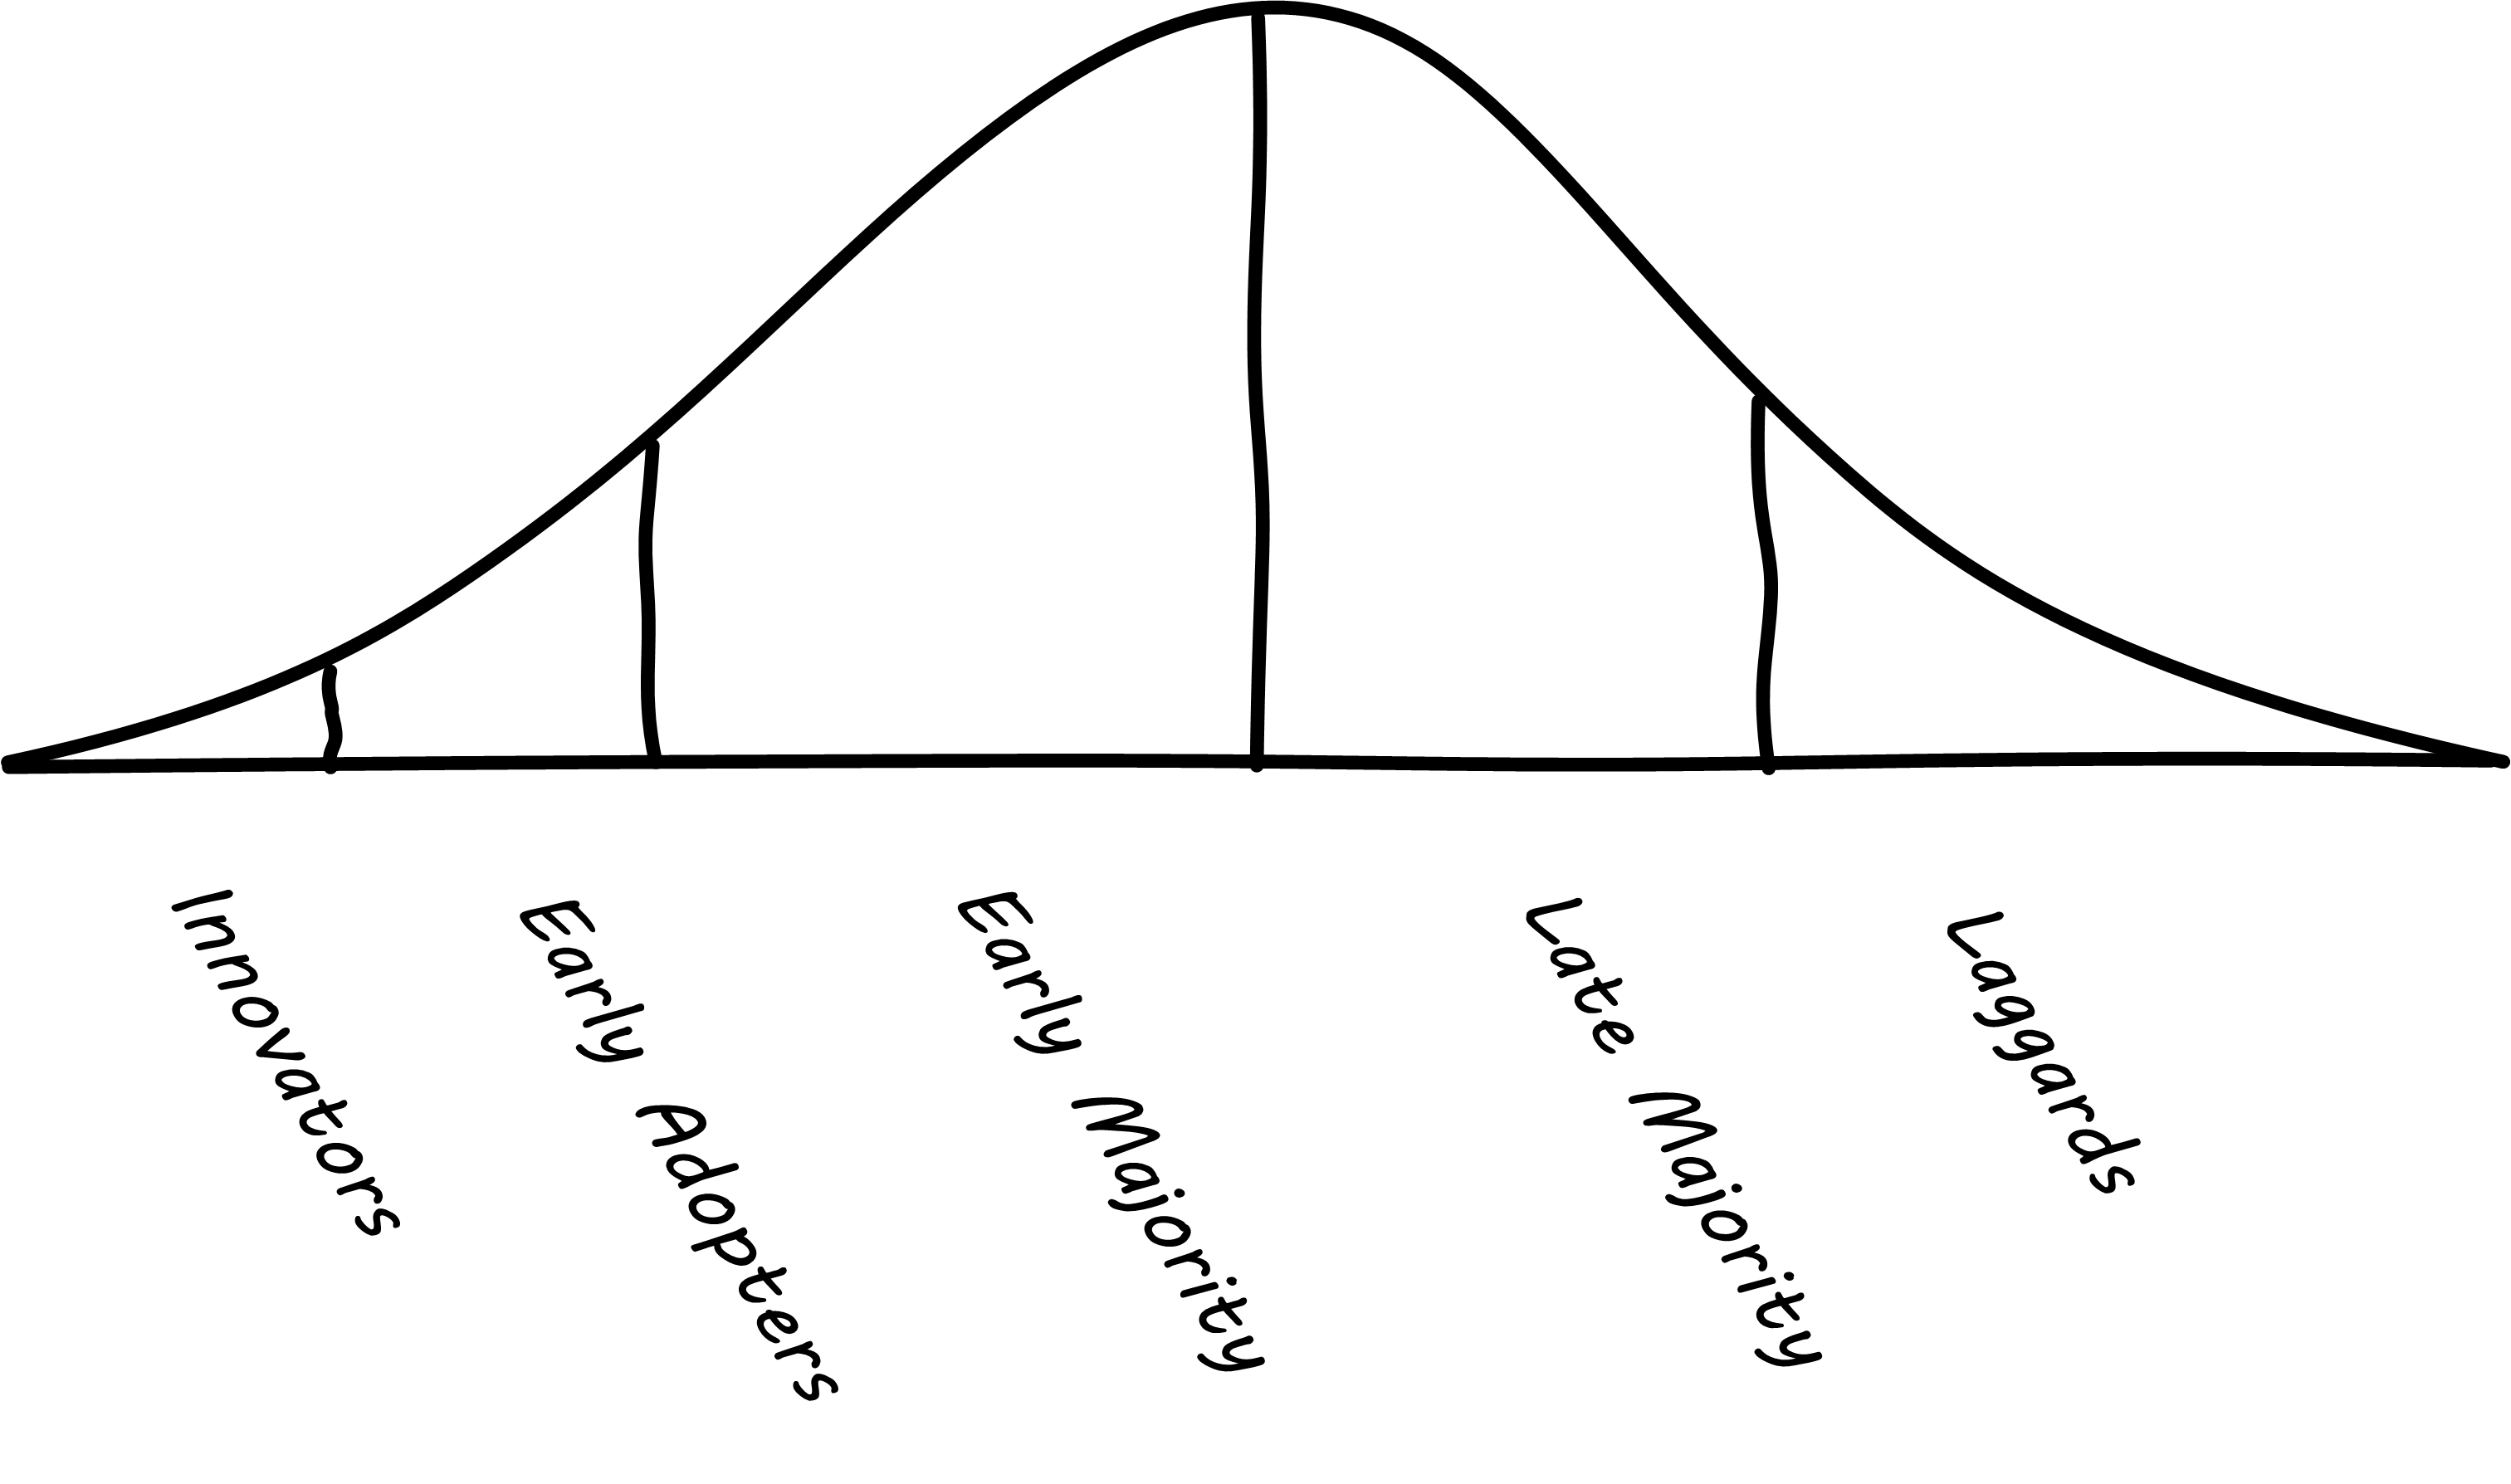
\includegraphics[width=0.48\textwidth]{images/1_01a-adoption.png}}}}{diffusion-{}graph}
\end{center}
\caption[{Technology adoption categories }]{Technology adoption categories \footnotemark{}}
\end{wrapfigure}
 
Rogers went on to characterize the various stages:
 \begin{itemize}

\item{} Innovators: Venturesome risk-{}takers
 

\item{} Early adopters: Opinion leaders
 

\item{} Early majority: Deliberative, numerous
 

\item{} Late majority: Skeptical, also numerous
 

\item{} Laggards: Traditional, isolated, conservative
 
\end{itemize}
 
The above figure was popularized in the following variation by Geoffrey Moore \hyperlink{Moore2014}{[Moore2014]} in his bestseller \emph{Crossing the Chasm}:
 \begin{wrapfigure}{r}{0.5\textwidth}[H]

\begin{center}
\imgexists{images/1_01-chasm.png}{{\imgevalsize{images/1_01-chasm.png}{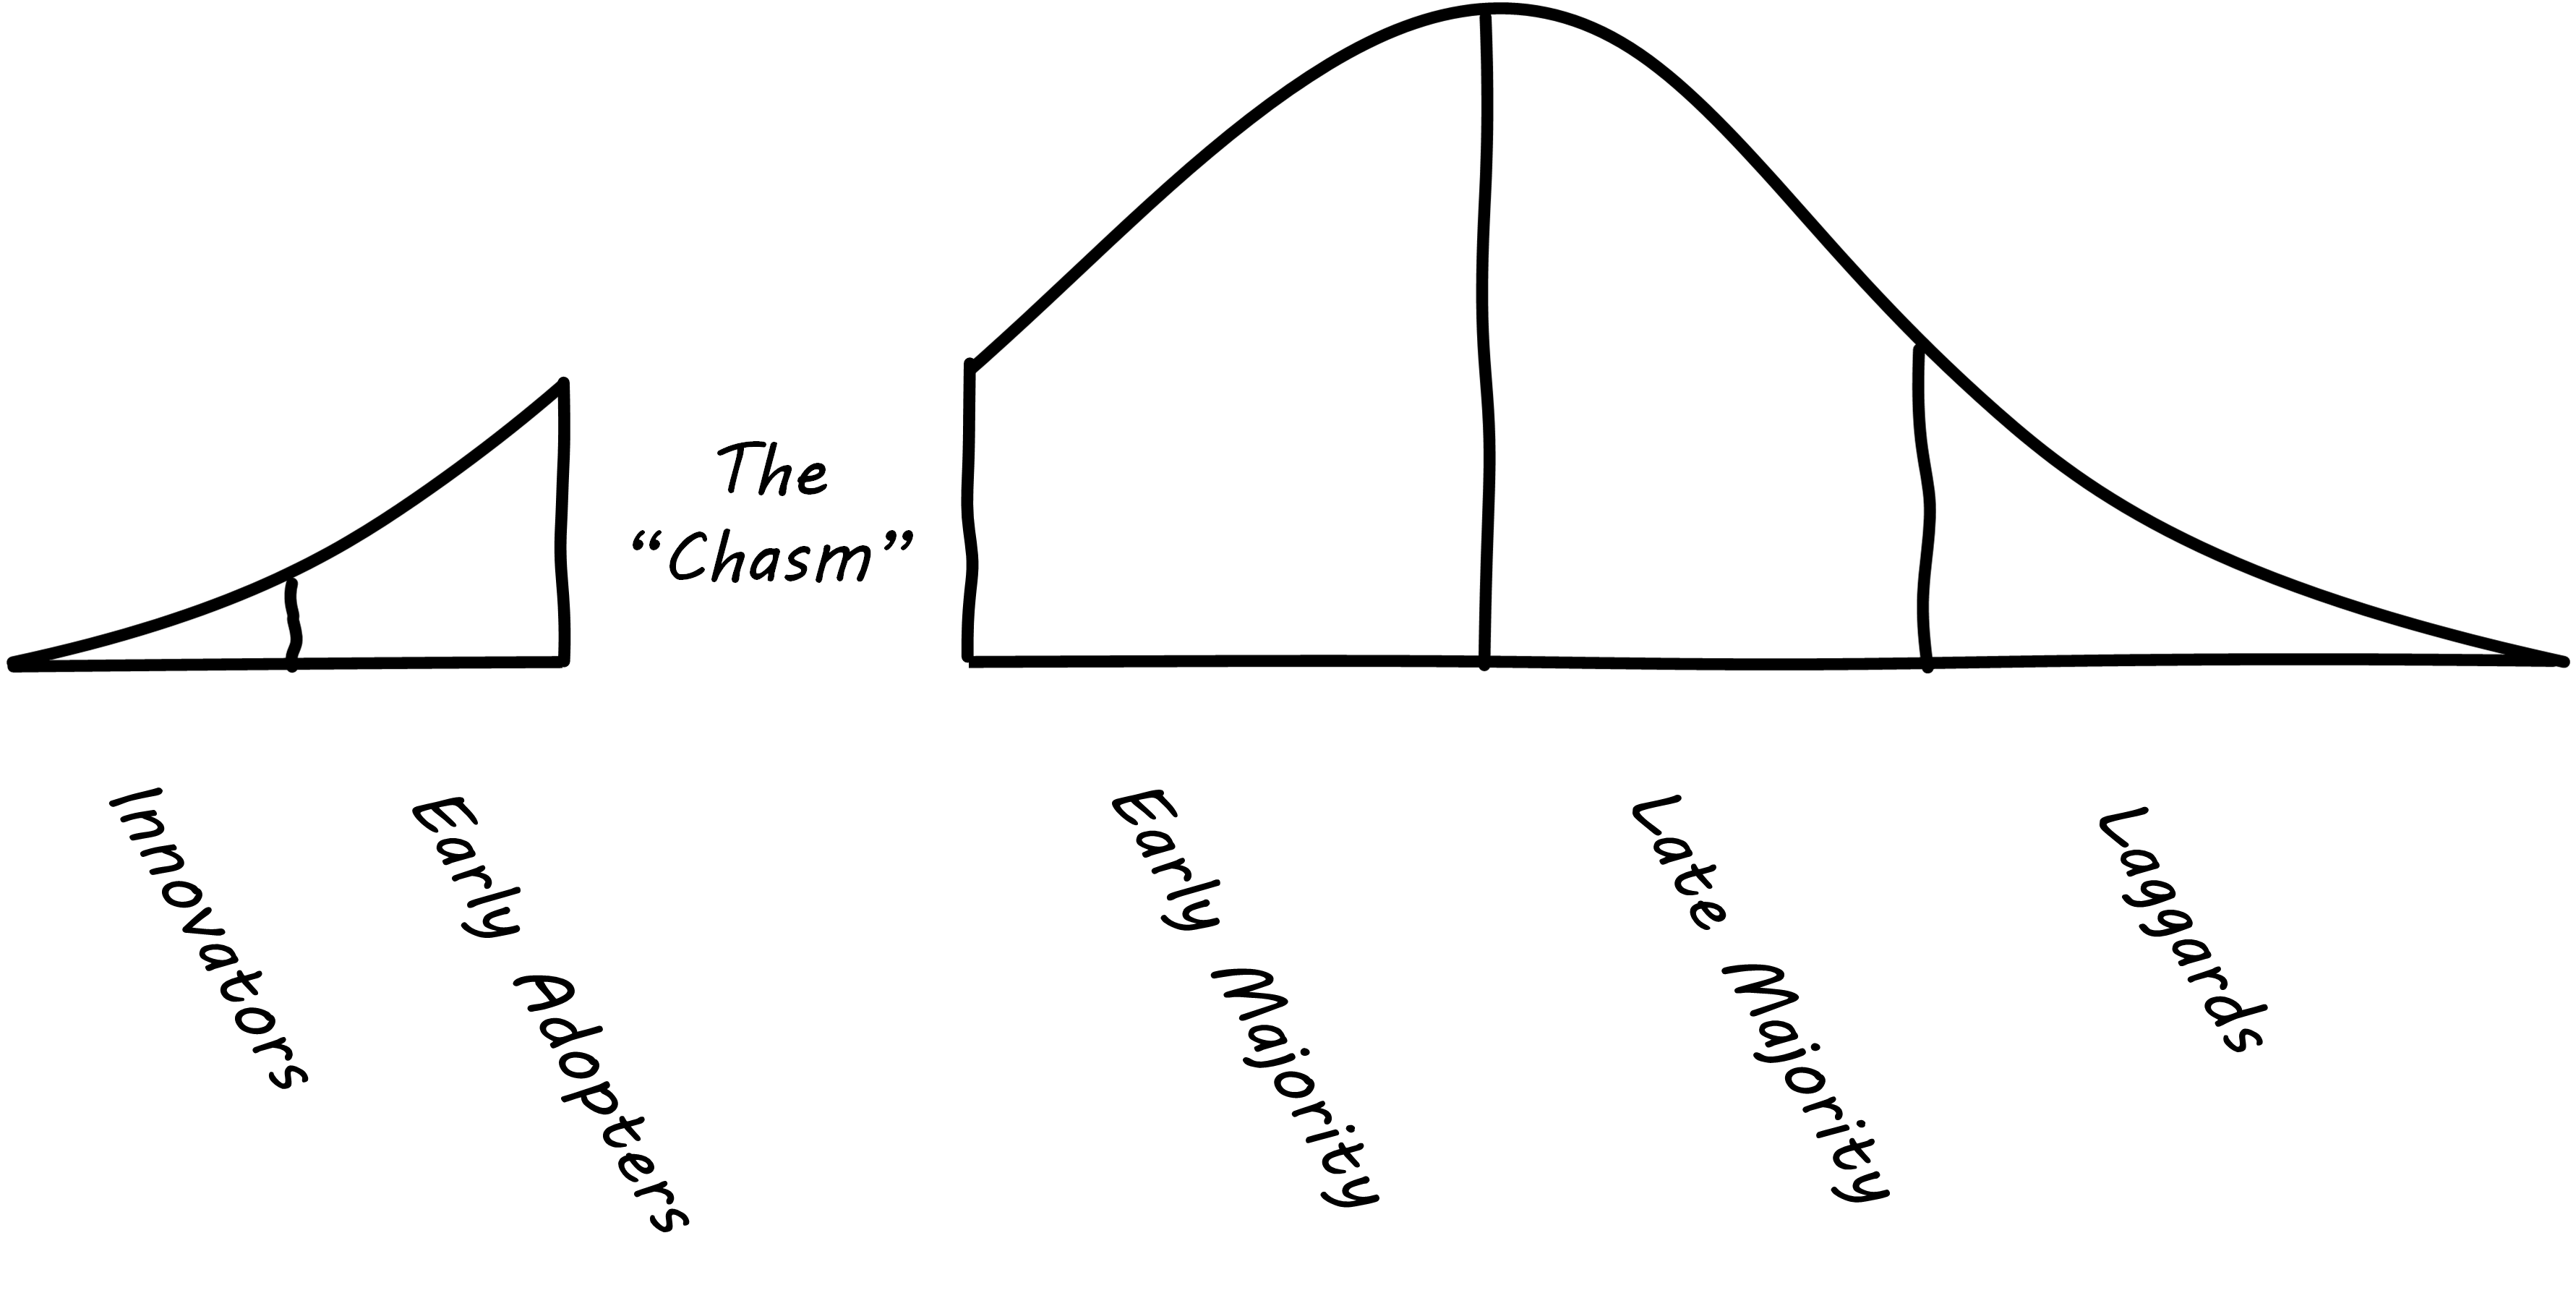
\includegraphics[width=0.48\textwidth]{images/1_01-chasm.png}}}}{chasm-{}graph}
\end{center}
\caption[{Purported "chasm" between adopter categories }]{Purported "chasm" between adopter categories \footnotemark{}}
\end{wrapfigure}
 
You'll see this diagram often, but you should be aware that Rogers himself (the person who has researched the data) says that (p.282):
 
\emph{Past research shows no support for this claim of a \textquotedblleft{}chasm\textquotedblright{} between certain adopter categories. On the contrary, innovativeness, if measured properly, is a continuous variable and there are no sharp breaks or discontinuities between adjacent adopter categories (although there are important differences between them)}.
 
The idea of technology diffusion frames the problem for us, but we need more. Steve Blank, in his influential book \emph{The Four Steps to Epiphany} \hyperlink{Blank2013}{[Blank2013]}, argues there are four categories for startups (p.31):
 \begin{itemize}

\item{} Startups that are entering an existing market
 

\item{} Startups that are creating an entirely new market
 

\item{} Startups that want to re-{}segment an existing market as a low-{}cost entrant
 

\item{} Startups that want to re-{}segment an existing market as a niche player
 
\end{itemize}
 
Understanding which category you are attempting is critical, because "the four types of startups have very different rates of customer adoption and acceptance."
 
Another related and well known categorization of competitive strategies comes from Michael Treacy and Fred Wiersma \hyperlink{Treacy1997}{[Treacy1997]}:
 \begin{itemize}

\item{} Customer intimacy
 

\item{} Product leadership
 

\item{} Operational excellence
 
\end{itemize}
 
It is not difficult to categorize well known brands in this way:
 \begin{table}[htbp]
\begin{center}
\begingroup%
\setlength{\newtblsparewidth}{\linewidth-2\tabcolsep-2\tabcolsep-2\tabcolsep-2\tabcolsep}%
\setlength{\newtblstarfactor}{\newtblsparewidth / \real{100}}%

\begin{tabular}{lll}\hline
\multicolumn{1}{|p{33.3333\newtblstarfactor}|}{\raggedright\bfseries%
%
Customer intimacy%
}&\multicolumn{1}{p{33.3333\newtblstarfactor}|}{\raggedright\bfseries%
%
Product leadership%
}&\multicolumn{1}{p{33.3334\newtblstarfactor}|}{\raggedright\bfseries%
%
Operational excellence%
}\tabularnewline
\cline{1-1}\cline{2-2}\cline{3-3}\multicolumn{1}{|p{33.3333\newtblstarfactor}|}{\raggedright%
Nordstrom Home Depot
%
}&\multicolumn{1}{p{33.3333\newtblstarfactor}|}{\raggedright%
Apple Nike
%
}&\multicolumn{1}{p{33.3334\newtblstarfactor}|}{\raggedright%
Dell Technologies Walmart
%
}\tabularnewline
\hline
\end{tabular}\endgroup%

\end{center}

\caption{Companies and their competitive strategies}
\end{table}
 
However, deciding which strategy to pursue as a startup may require some experimentation.
  
\subsubsection{Business discovery approaches}
\label{_business_discovery_approaches}\hyperlabel{_business_discovery_approaches}%
  \begin{quote}

Startups that survive the first few tough years do not follow the traditional product-{}centric launch model espoused by product managers or the venture capital community\ldots{}\hspace{0em}In particular, the winners invent and live by a process of customer learning and discovery. I call this process \textquotedblleft{}Customer Development,\textquotedblright{} a sibling to \textquotedblleft{}Product Development,\textquotedblright{} and each and every startup that succeeds recapitulates it, knowingly or not.

\hspace*\fill--- Steve Blank
\emph{The Four Steps to Epiphany} \end{quote}
 
Let's start with two well known approaches that can help you bridge from an understanding of your product context, to an effective vision for building and sustaining a product:
 \begin{itemize}

\item{} Alexander Osterwalder's Business Model Canvas
 

\item{} Eric Ries' Lean Startup
 
\end{itemize}
 
\label{biz-model-canvas}\hyperlabel{biz-model-canvas}
 
\paragraph{Business model canvas}
\label{_business_model_canvas}\hyperlabel{_business_model_canvas}%
  
One recent book that's been influential among enterpreneurs is Alex Osterwalder's \emph{Business Model Generation} \hyperlink{Osterwalder2010}{[Osterwalder2010]}.
 
This book is perhaps best known for introducing the concept of the Business Model Canvas, which it defines as "A shared language for describing, visualizing, assessing, and changing business models."
 
The Business Model Canvas uses 9 major categories to describe the business model:
 \begin{itemize}

\item{} Key Partners
 

\item{} Key Activities
 

\item{} Value Proposition
 

\item{} Customer Relationships
 

\item{} Customer Segments
 

\item{} Key Resources
 

\item{} Channels
 

\item{} Cost Structure
 

\item{} Revenue Streams
 
\end{itemize}
 
and suggests they be visualized in this manner:
 \begin{wrapfigure}{r}{0.5\textwidth}[H]

\begin{center}
\imgexists{images/1_01-BizModelCanvas.png}{{\imgevalsize{images/1_01-BizModelCanvas.png}{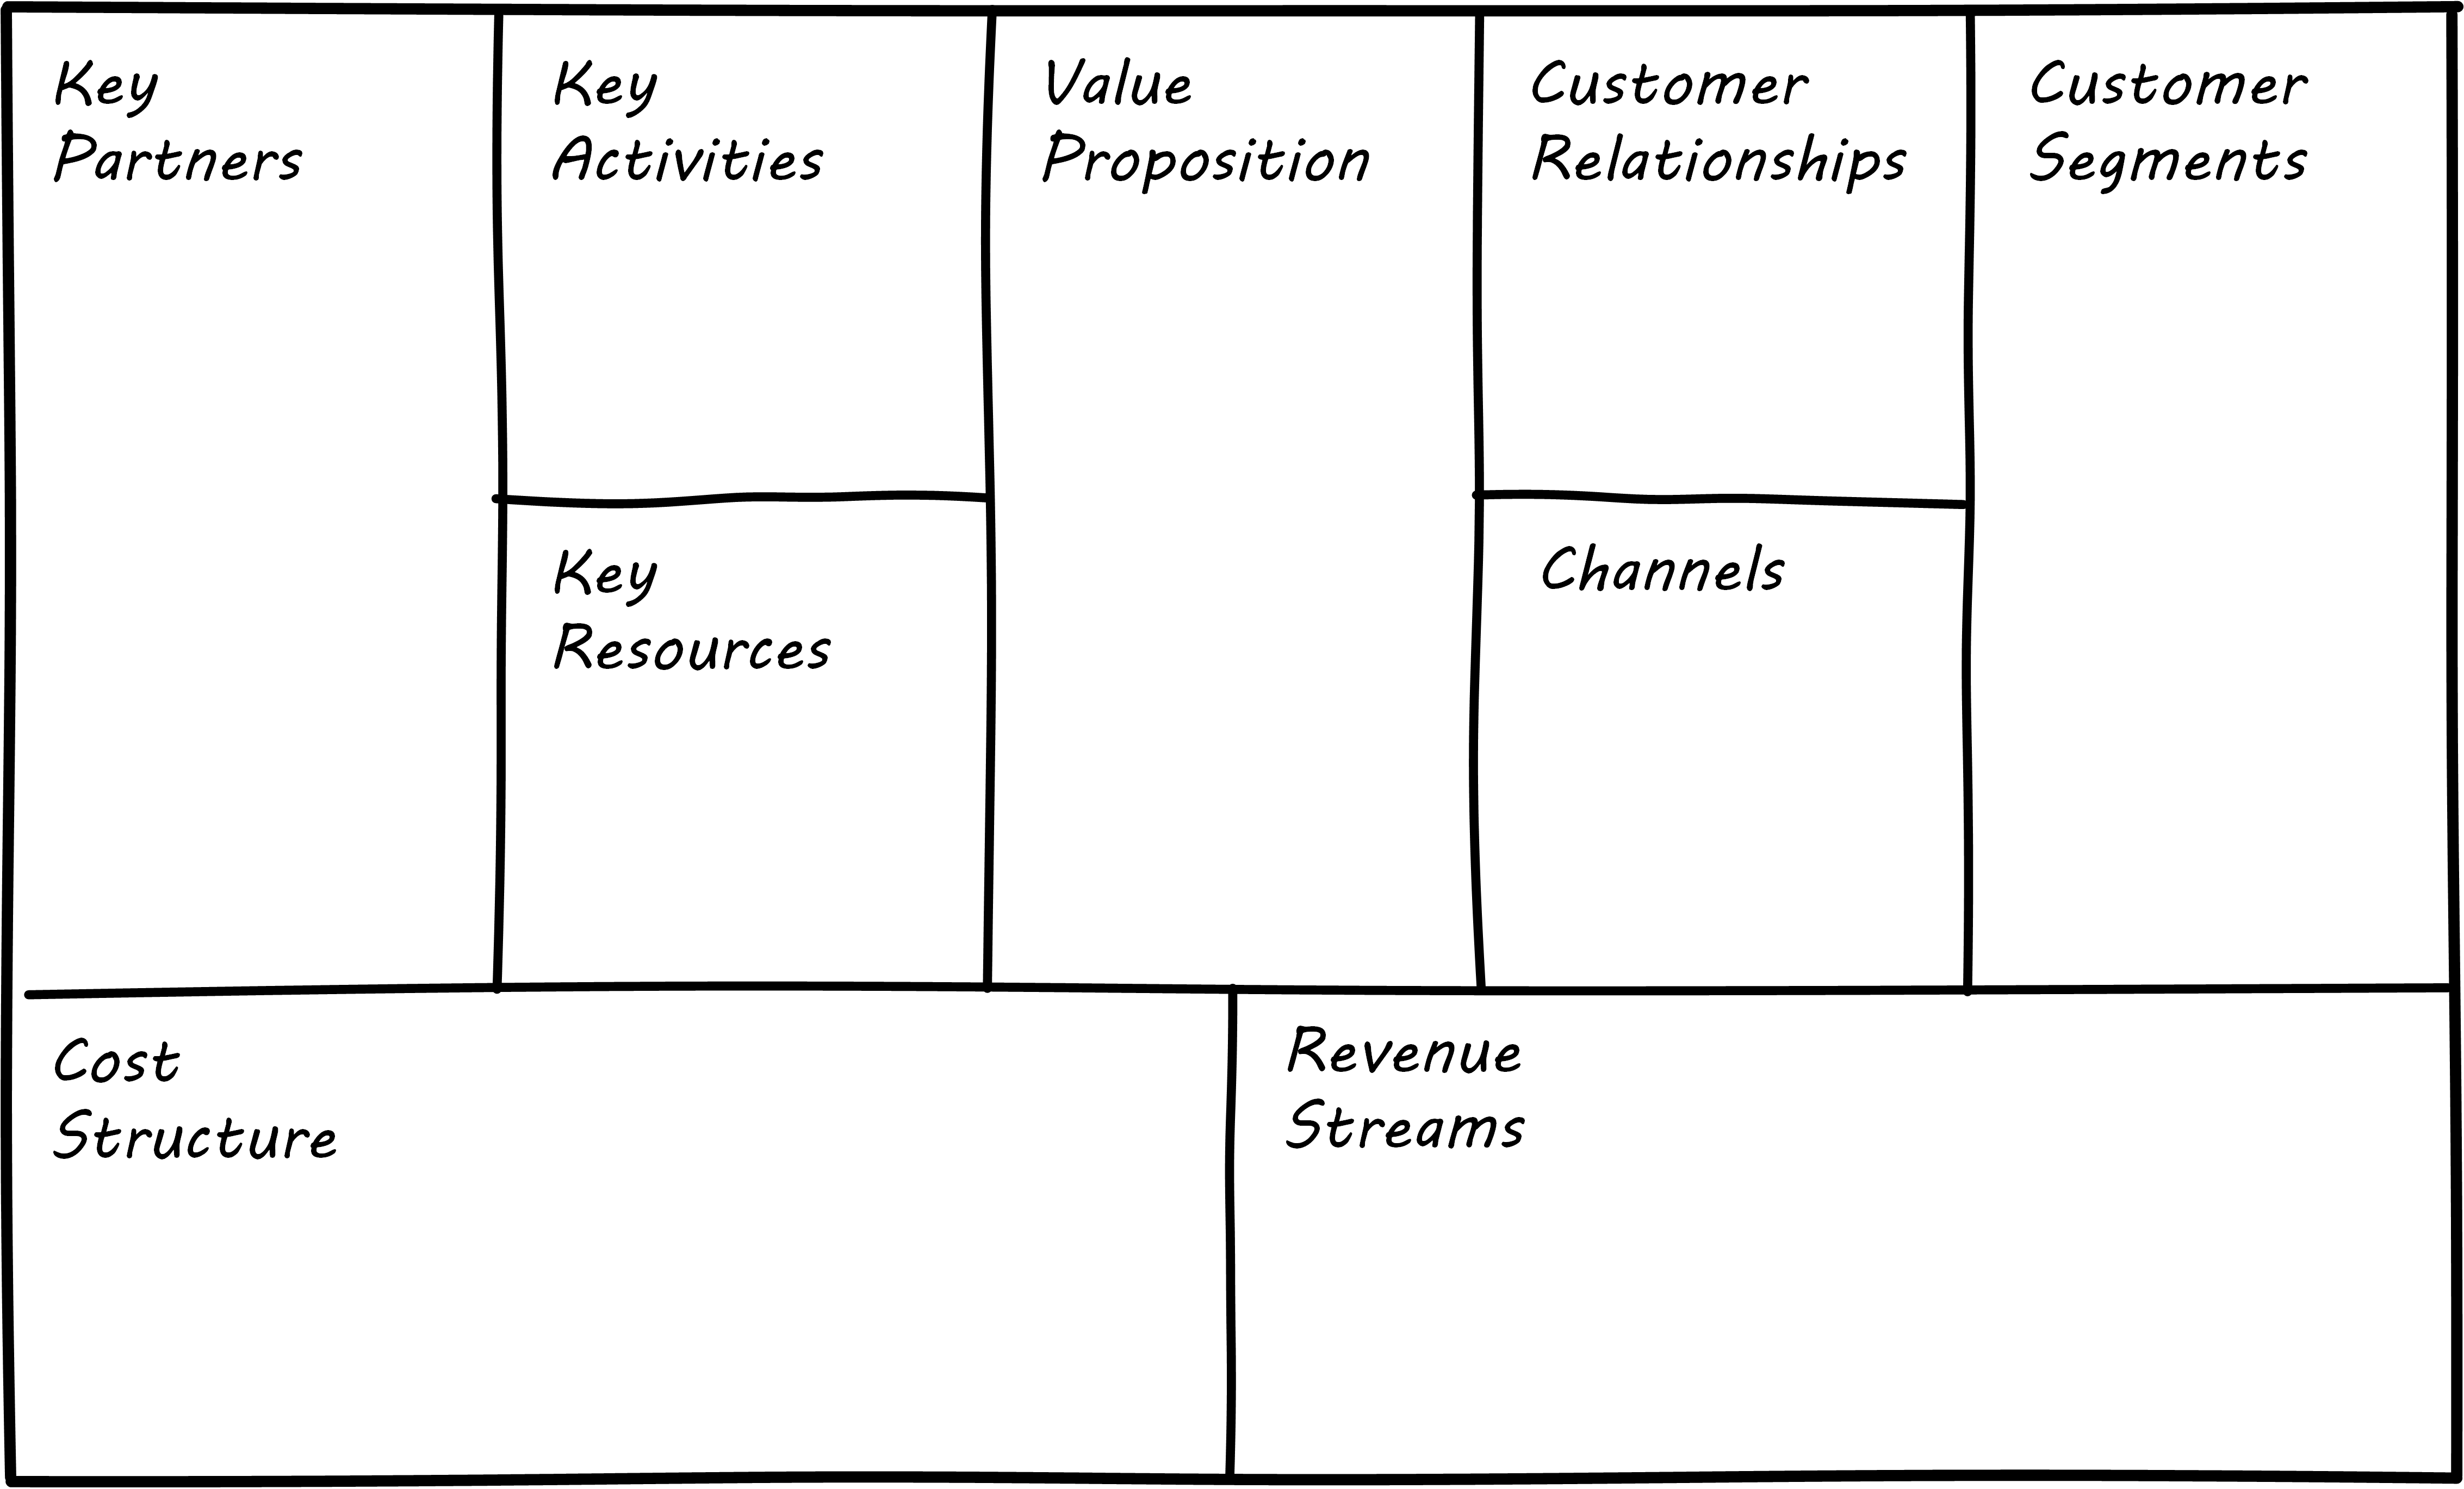
\includegraphics[width=0.48\textwidth]{images/1_01-BizModelCanvas.png}}}}{business model canvas}
\end{center}
\caption[{Business Model Canvas (similar to [Osterwalder2010], p. 44)}]{Business Model Canvas (\emph{similar to \hyperlink{Osterwalder2010}{[Osterwalder2010]}, p. 44})}
\end{wrapfigure}
 
The canvas is then used in collaborative planning, e.g. as a large format wall poster where the business team can brainstorm, discuss, and fill in the boxes (e.g., what is the main "Value Proposition"? Mobile bank account access?):
 \begin{wrapfigure}{r}{0.5\textwidth}[H]

\begin{center}
\imgexists{images/1_01-BMC-example.png}{{\imgevalsize{images/1_01-BMC-example.png}{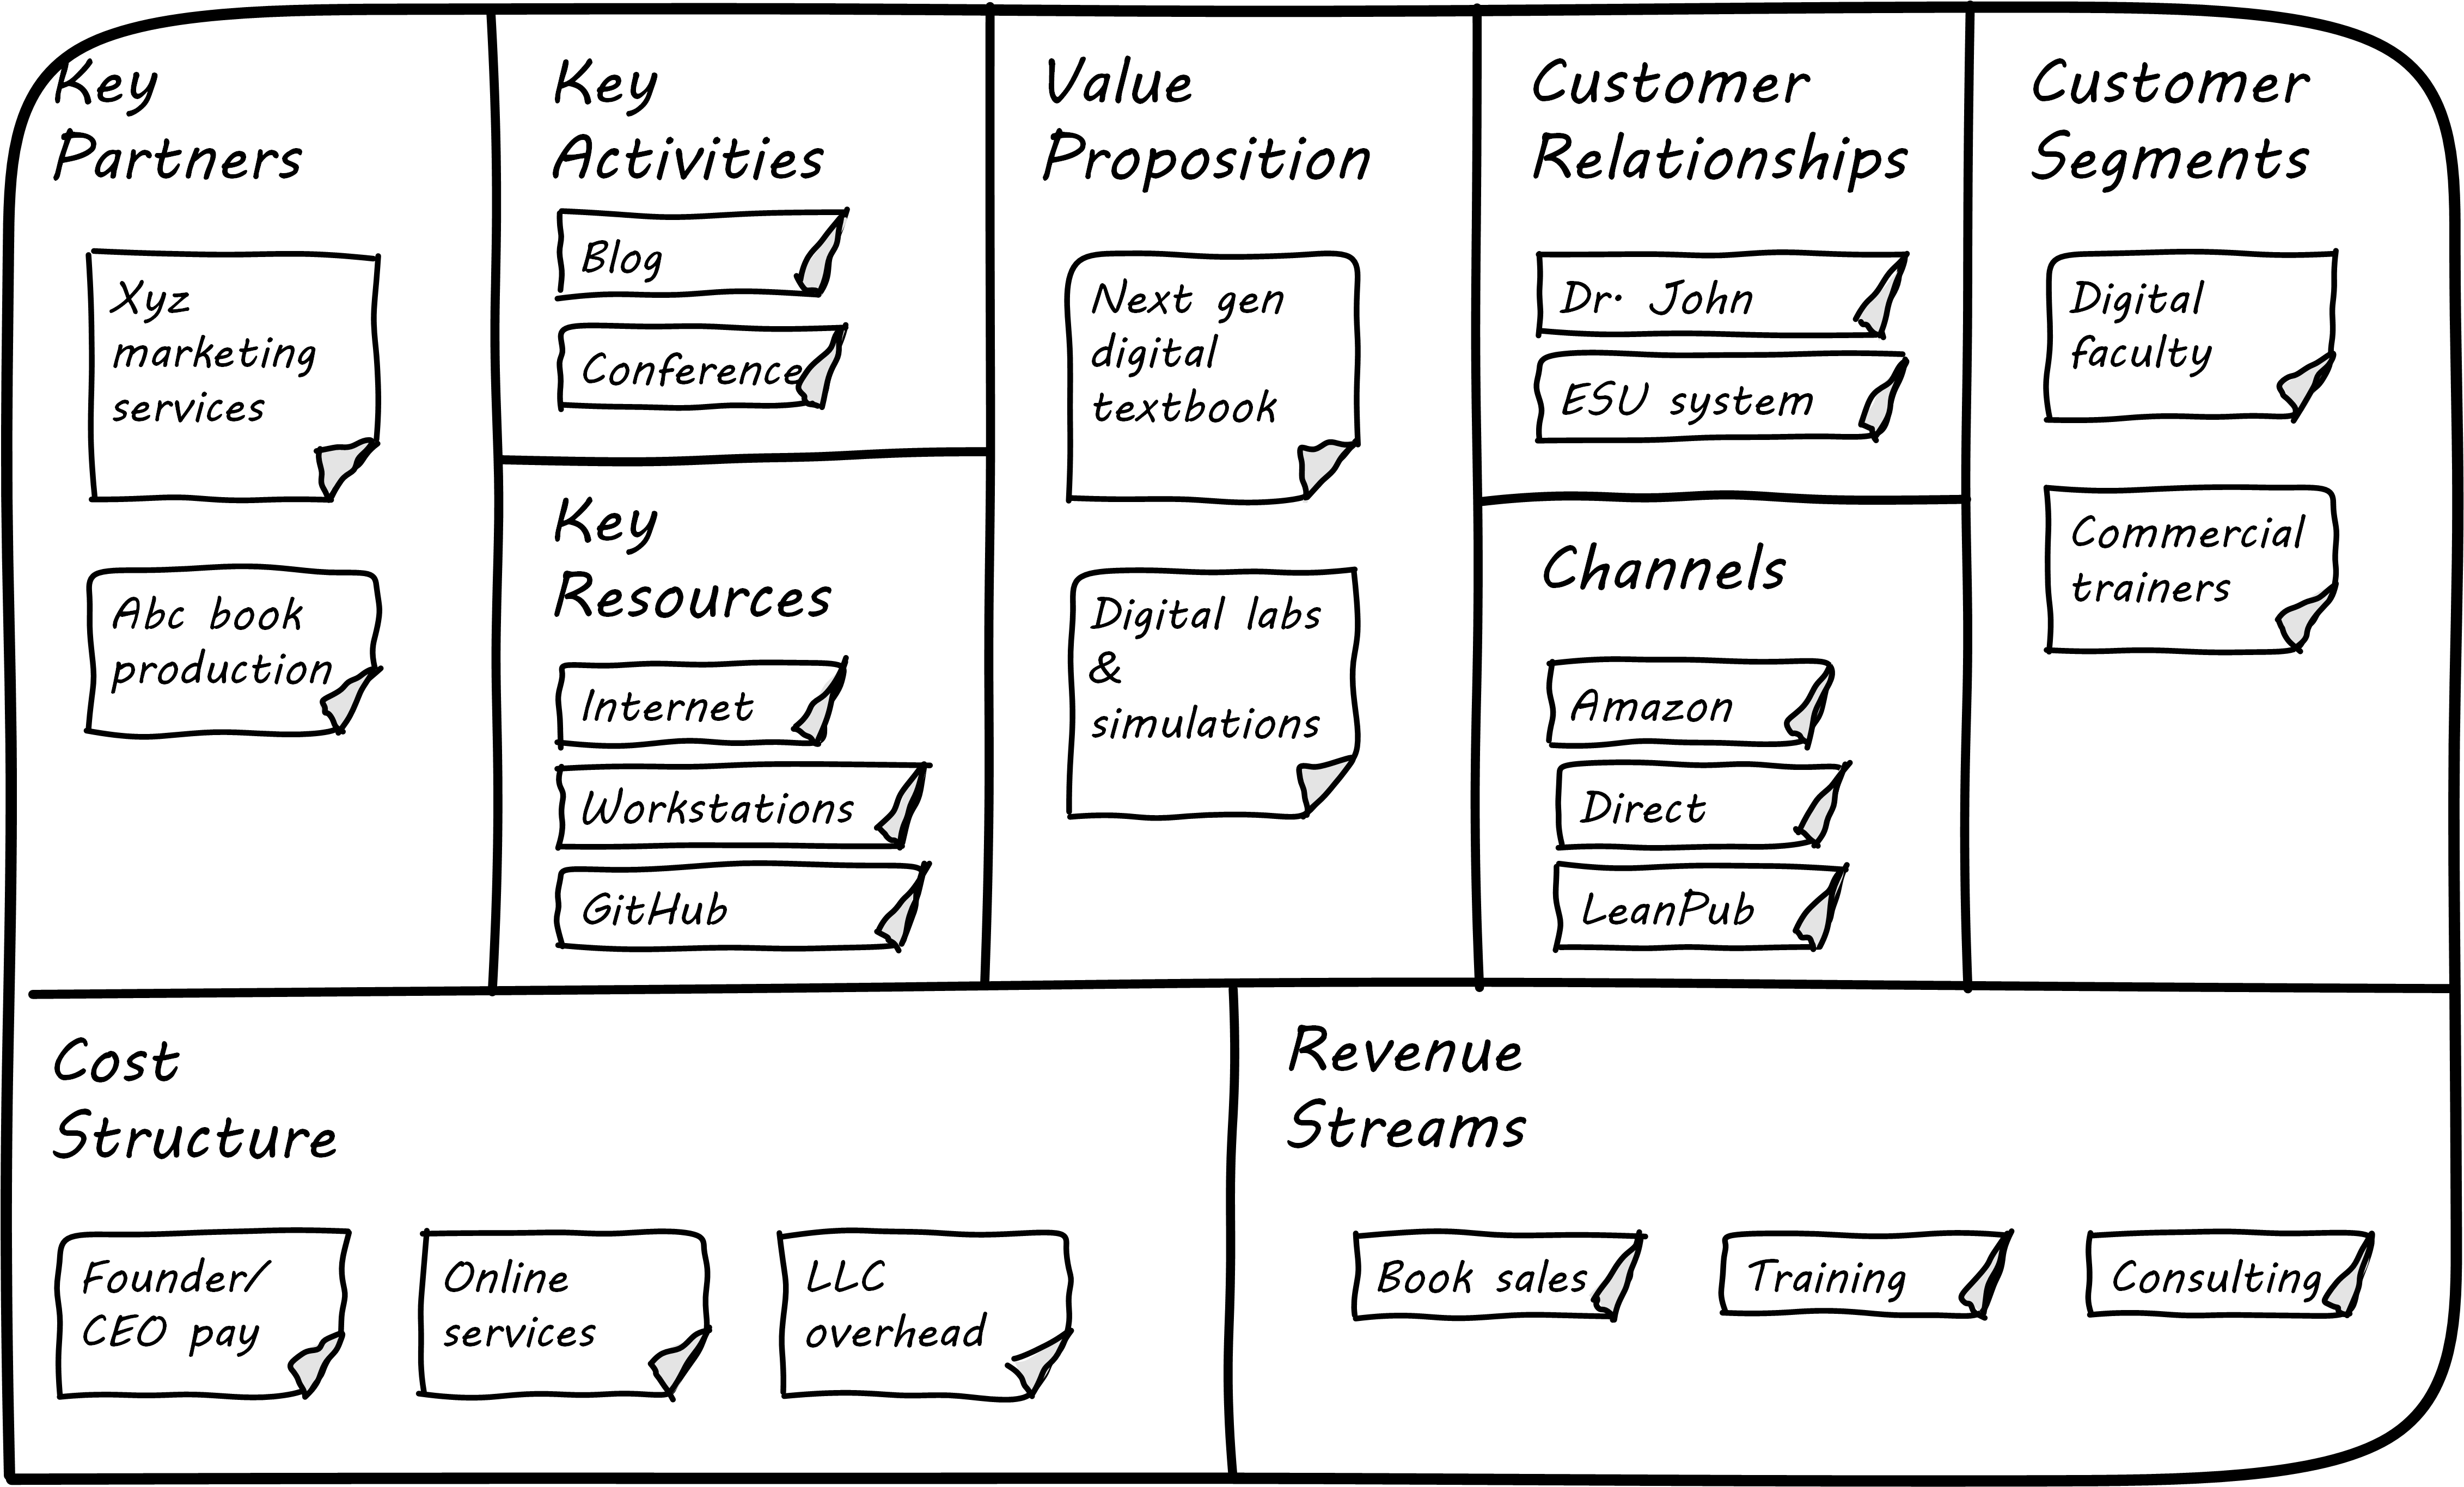
\includegraphics[width=0.48\textwidth]{images/1_01-BMC-example.png}}}}{author's business model canvas}
\end{center}
\caption{A rough approximation of the author's business model on the Business Model Canvas}
\end{wrapfigure}
 
Osterwalder and his colleagues, in \emph{Business Model Generation} and the followup \emph{Value Proposition Design} \hyperlink{Osterwalder2014}{[Osterwalder2014]}, suggest a wide variety of imaginative and creative approaches to developing business models and value propositions, in terms of patterns, processes, design approaches, and overall strategy.
 
\label{business-case-analysis}\hyperlabel{business-case-analysis}
  
\paragraph{Business case analysis}
\label{_business_case_analysis}\hyperlabel{_business_case_analysis}%
  
There are a wide variety of analysis techniques for making a business case at a more detailed level. Donald Reifer, in \emph{Making the Software Business Case} \hyperlink{Reifer2002}{[Reifer2002]}, lists:
 \begin{itemize}

\item{} Breakeven analysis
 

\item{} Cause-{}and-{}effect analysis
 

\item{} Cost/benefit analysis
 

\item{} Value chain analysis
 

\item{} Investment opportunity analysis
 

\item{} Pareto analysis
 

\item{} Payback analysis
 

\item{} Sensitivity analysis
 

\item{} Trend analysis
 
\end{itemize}
 
A primary theme of this book is that empirical, experimental approaches are essential to digital management. Any analysis, carried to an extreme without a sound basis in real data, risks becoming a "castle in the air." But when you are putting real money on the line (even the opportunity costs of the time you are spending on your startup), it is advisable to look at the decision from various perspectives. These techniques can be useful for that purpose. However, once you have some indication there might be business value in a given idea, applying Lean Startup techniques may be more valuable than continuing to analyze.
 
\label{lean-startup}\hyperlabel{lean-startup}
  
\paragraph{Lean Startup}
\label{_lean_startup}\hyperlabel{_lean_startup}%
  \begin{quote}

The goal of a startup is to figure out the right thing to build\textemdash{} the thing customers want and will pay for\textemdash{} as quickly as possible. In other words, the Lean Startup is a new way of looking at the development of innovative new products that emphasizes fast iteration and customer insight, a huge vision, and great ambition, all at the same time.

\hspace*\fill--- Eric Ries
\emph{The Lean Startup} \end{quote}
 \begin{wrapfigure}{r}{0.5\textwidth}[H]

\begin{center}
\imgexists{images/1_01-leanStartup.png}{{\imgevalsize{images/1_01-leanStartup.png}{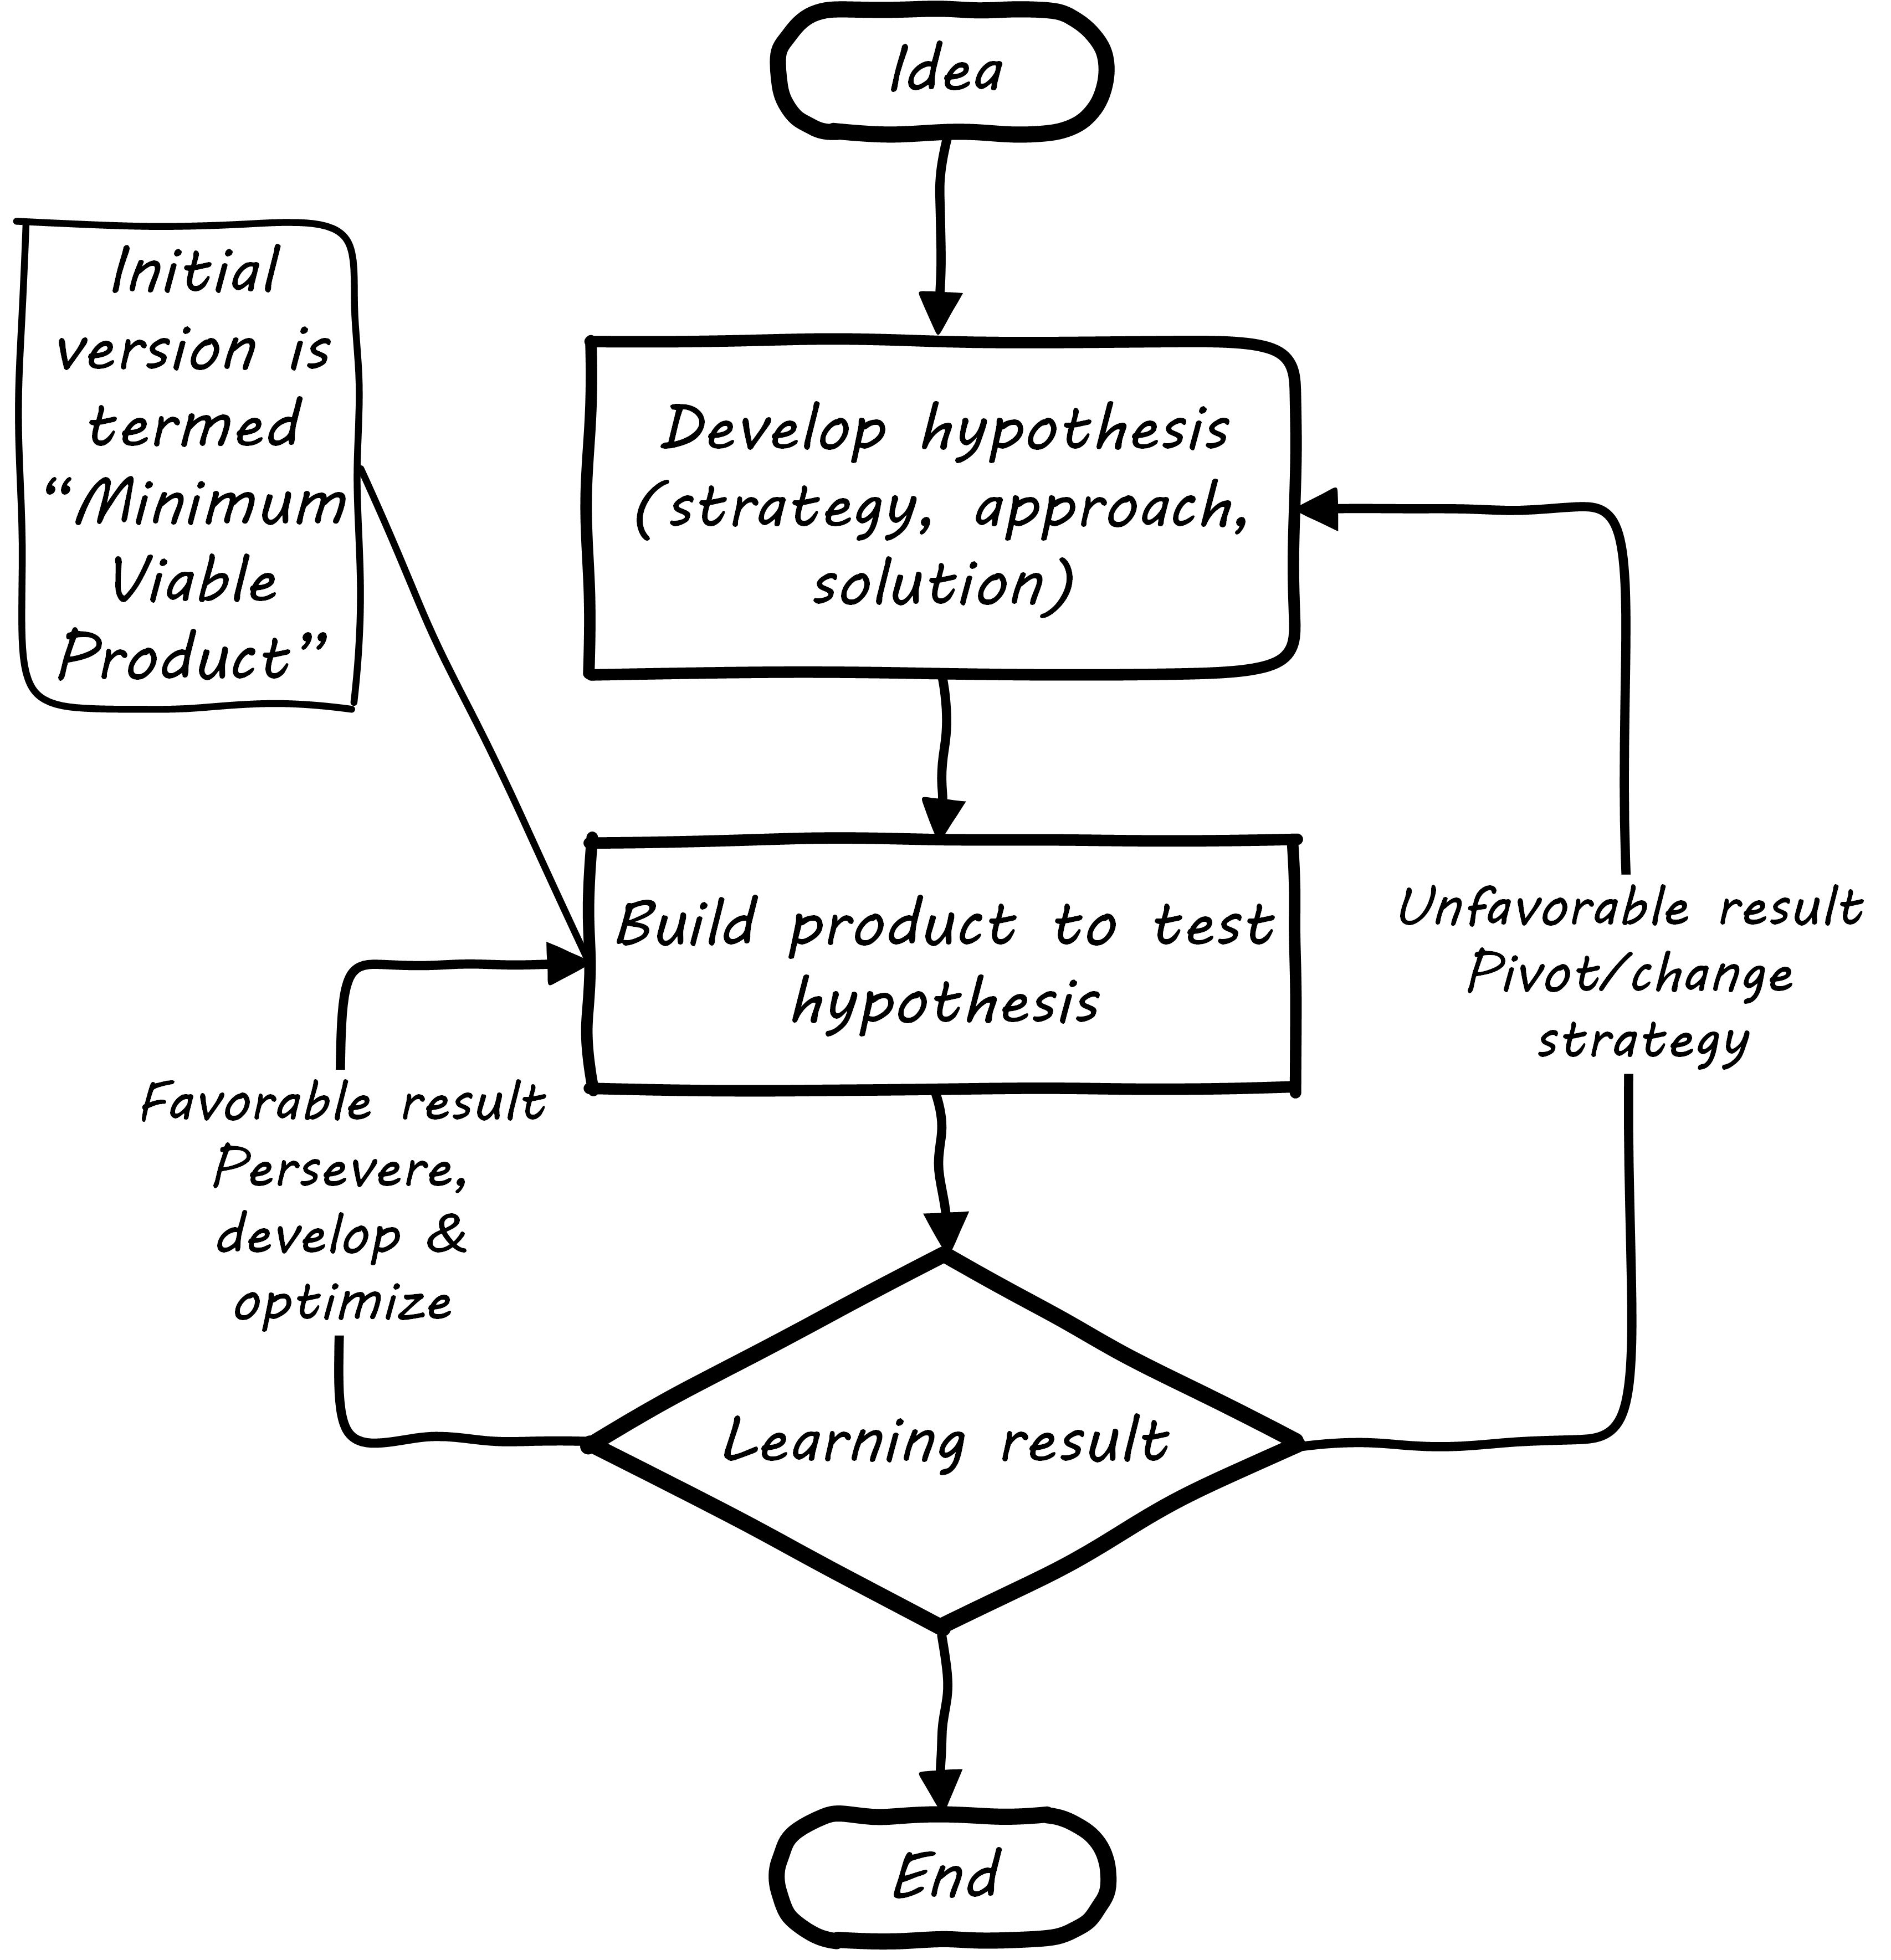
\includegraphics[width=0.48\textwidth]{images/1_01-leanStartup.png}}}}{Lean Startup flowchart}
\end{center}
\caption{Lean Startup flowchart}
\end{wrapfigure}
 
Lean Startup is a philosophy of entrepreneurship developed by Eric Ries \hyperlink{Ries2011}{[Ries2011]}. It is not specific to information technology; rather, it is broadly applicable to all attempts to understand a product and its market. (Remember according to our \hyperlink{prod-mgmt-definition}{definition of product management} that a workable market position is essential to any product.)
 
The idea of the Lean Startup has had profound influence on product design, including market-{}facing and even internal IT systems. It is grounded in Agile concepts such as:
 
"Do the simplest thing that could possibly work."
 
Lean Startup calls for an iterative, "Build-{}Measure-{}Learn" cycle. Repeating this cycle frequently is the essential process of building a successful startup (whatever the digital proportion).
 \begin{itemize}

\item{} Develop an idea for a Minimum Viable Product (MVP)
 

\item{} Measure its effectiveness in the market (internal/external)
 

\item{} Learn from the experiment
 

\item{} Decide to persevere or pivot (change direction while leveraging momentum)
 

\item{} New idea development, evolution of MVP
 
\end{itemize}
 
Flowcharts such as the one shown are often seen to describe the Lean Startup process. We will go into much more depth on product management in Chapter 4 and Part III.
 
Bente notes that Broadbent and Kitzis (2005) distinguish three fundamental business outlooks-{} fighting for survival, maintaining competitiveness, breaking away
   
\subsubsection{The enterprise context}
\label{_the_enterprise_context}\hyperlabel{_the_enterprise_context}%
  
\begin{lstlisting}[firstnumber=1,backgroundcolor={},basicstyle=\ttfamily,]
We will discuss in Chapter 12. For now, assume that your role and priorities are defined by some strategic planning and investment activities. You need to understand the mission to the best of your abilities, even as an individual contributor. This book will take you through the journey of understanding how such priorities are set.
\end{lstlisting}
 
\begin{lstlisting}[firstnumber=1,backgroundcolor={},basicstyle=\ttfamily,]
important - commentary on Agile Product Roadmap - arrow https://twitter.com/ScrumDan/status/786729964422909953
\end{lstlisting}
 
\begin{lstlisting}[firstnumber=1,backgroundcolor={},basicstyle=\ttfamily,]
when do they become explicit?
\end{lstlisting}
  
\subsubsection{Current digital business trends}
\label{_current_digital_business_trends}\hyperlabel{_current_digital_business_trends}%
  

\begin{sidebar}

\textbf{Sidebar: The Digital Services Playbook} Understand what people need
Address the whole experience, from start to finish
Make it simple and intuitive
Build the service using agile and iterative practices
Structure budgets and contracts to support delivery
Assign one leader and hold that person accountable
Bring in experienced teams
Choose a modern technology stack
Deploy in a flexible hosting environment
Automate testing and deployments
Manage security and privacy through reusable processes
Use data to drive decisions
Default to open
\end{sidebar}
 
\paragraph{Apps}
\label{_apps}\hyperlabel{_apps}%
    
\paragraph{Big Data}
\label{_big_data}\hyperlabel{_big_data}%
    
\paragraph{Internet of Things}
\label{_internet_of_things}\hyperlabel{_internet_of_things}%
    
\paragraph{Platforms not products}
\label{_platforms_not_products}\hyperlabel{_platforms_not_products}%
  
\begin{lstlisting}[firstnumber=1,backgroundcolor={},basicstyle=\ttfamily,]
Bring in Rauser: Digital Strategy: A Guide to Digital Business Transformation, Rogers: The Digital Transformation Playbook: Rethink Your Business for the Digital Age, and Westerman various.
\end{lstlisting}
 
\begin{lstlisting}[firstnumber=1,backgroundcolor={},basicstyle=\ttfamily,]
"Post-industrialism turns brand management into a digital conversation between a company and its customers." <<Sussna2015>>
\end{lstlisting}
 
\begin{lstlisting}[firstnumber=1,backgroundcolor={},basicstyle=\ttfamily,]
images
\end{lstlisting}
 
\begin{lstlisting}[firstnumber=1,backgroundcolor={},basicstyle=\ttfamily,]
https://www.flickr.com/photos/usnavy/28073762161
\end{lstlisting}
 \begin{itemize}

\item{} demand vs. supply
 

\item{} problem vs. solution
 

\item{} outside-{}in vs. inside-{}out thinking
 

\item{} service vs. system
 

\item{} black-{}box vs glass box
 
\end{itemize}
    
\subsection{Conclusion}
\label{Chap1-Conclusion}\hyperlabel{Chap1-Conclusion}%
  
In this chapter, we discussed the basic questions of information technology value and how it is experienced and developed. Through the mechanism of a hypothetical modern IT user, we covered (at a \textbf{very} high level) the necessary ingredients of the IT experience. We considered the user's moment of truth, and the massive IT complexity that sustains it. We also discussed a high level lifecycle model for IT applications and services, and explored some initial definitions for user, customer, and sponsor -{} critical distinctions to make in an age of digital transformation.
 
As you proceed into the course, the key takeway from this chapter is "why IT?" Why do people need it, and how is it valuable? That should always remain at the top of your mind as you proceed in your IT education.
 
\subsubsection{Discussion questions}
\label{_discussion_questions}\hyperlabel{_discussion_questions}%
  \begin{enumerate}[label=\arabic*.]

\item{} Discuss: How does information technology contribute to your enjoyment of life and experiences of value?
 

\item{} Read \href{http://www.wsj.com/news/articles/SB20001424052702303743604579350710633713786}{Apps Are Wrecking Mom-{}and-{}Pop Pizza Shops} and discuss whether "IT matters" to the local pizzerias.
 

\item{} Read the Wikipedia articles on \href{https://en.wikipedia.org/wiki/Mainframe_computer}{mainframe computing} and \href{https://en.wikipedia.org/wiki/Amazon_Web_Services}{Amazon Web Services} and discuss with your team. What has changed in computing? What remains the same?
 
\end{enumerate}
  
\subsubsection{Research \& practice}
\label{_research_practice}\hyperlabel{_research_practice}%
  \begin{enumerate}[label=\arabic*.]

\item{} Go to any popular online service (Facebook, Netflix, Flickr, etc.) How would you describe the "moments of truth" or value experiences these sites offer users? There may be several.
 

\item{} On your own or with a team, develop an idea for an IT-{}based product you could take to market. Present to the class.
 

\item{} (Continued) Who are the user, customer, and sponsor of your product?
 

\item{} Research and apply one of the \hyperlink{business-case-analysis}{business case analysis techniques} to your idea.
 
\end{enumerate}
  
\subsubsection{Further reading}
\label{_further_reading}\hyperlabel{_further_reading}%
  
\textbf{Books}
 \begin{itemize}

\item{} \href{http://www.amazon.com/Code-Language-Computer-Hardware-Software/dp/0735611319}{\emph{Code}}, Charles Petzold
 

\item{} \href{http://www.amazon.com/Information-History-Theory-Flood/dp/1400096235/ref=sr_1_1?s=books&ie=UTF8&qid=1438398170&sr=1-1&keywords=the+information}{\emph{The Information,}} James Glieck
 

\item{} \href{http://www.amazon.com/Lean-Startup-Entrepreneurs-Continuous-Innovation-ebook/dp/B004J4XGN6/ref=sr_1_1?s=books&ie=UTF8&qid=1438398231&sr=1-1&keywords=the+lean+startup}{\emph{The Lean Startup}}, Ries
 
\end{itemize}
 
\textbf{Articles}
 \begin{itemize}

\item{} \href{https://en.wikipedia.org/wiki/Technology_stack}{definitions of IT stack} (follow links)
 

\item{} \href{http://www.nytimes.com/2014/12/01/business/working-the-land-and-the-data.html?smid=tw-share&_r=0}{Working the Land and the Data}
 

\item{} \href{https://en.wikipedia.org/wiki/Outside%E2%80%93in_software_development}{Outside-{}in software development}
 
\end{itemize}
 
\label{chapter-2}\hyperlabel{chapter-2}
    
\section{Chapter 2: Infrastructure Management}
\label{_chapter_2_infrastructure_management}\hyperlabel{_chapter_2_infrastructure_management}%
  
\subsection{Introduction}
\label{_introduction_2}\hyperlabel{_introduction_2}%
  

\begin{sidebar}

\textbf{Collaborative}

Status 2016-{}11-{}2016: This chapter is in "draft 1.5" -{} improved from original first draft completed in 2015.

\emph{There is a wealth of material covering IT infrastructure in far more detail than possible here. We don't want to rewrite Morris, Allspaw or Limoncelli. Curating the most useful aspects for a survey text is the challenge.}

\emph{Note that Chapter 6 is dedicated to IT operations.}
\begin{itemize}

\item{} Raise an \href{https://github.com/dm-academy/aitm/issues}{issue} to comment
 

\item{} \href{https://raw.githubusercontent.com/dm-academy/aitm/master/book/PATH_TO_FILE.adoc}{Github source}
 

\item{} \href{https://github.com/dm-academy/aitm/blob/master/collaborator-instructions.adoc}{Collaborator instructions}
 
\end{itemize}

\emph{Collaboration notes}
\end{sidebar}
 \begin{wrapfigure}{r}{0.5\textwidth}[H]

\begin{center}
\imgexists{images/1_02-data-center.jpg}{{\imgevalsize{images/1_02-data-center.jpg}{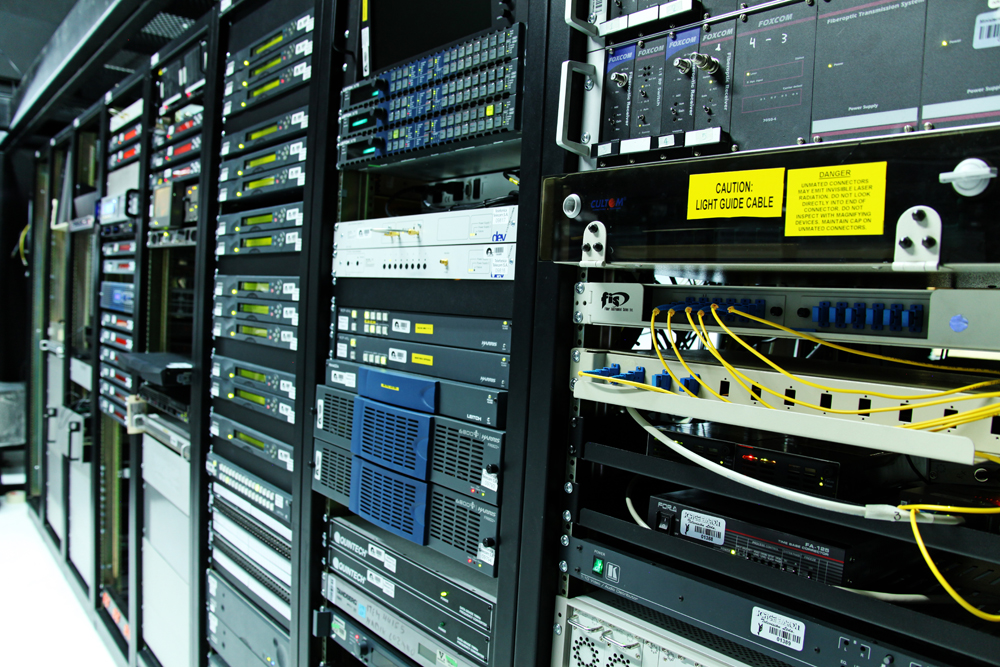
\includegraphics[width=0.48\textwidth]{images/1_02-data-center.jpg}}}}{equipment in racks}
\end{center}
\caption[{Racks in a data center }]{Racks in a data center \footnotemark{}}
\end{wrapfigure}
 
As mentioned in the Part Introduction, you cannot start developing a product until you decide what you will build it with. (You may have a difficult time writing an app for a mobile phone if you choose the COBOL programming language!)  You also need to understand something of how computers are operated, enough so that you can make decisions on how your system will run. Most startups choose to run IT services on infrastructure owned by a Cloud provider, but there are other options. Certainly, as you scale up, you'll need to be more and more sophisticated in your understanding of your underlying IT services.
 
Configuring your base platform is one of the most important capabilities you will need to develop. You'll never stop doing it. The basis of modern configuration management is \href{https://en.wikipedia.org/wiki/Version_control}{version control}, which we cover here.
 
This is one of the more technical chapters. Supplementary reading may be required for those completely unfamiliar with computing. See \hyperlink{reader-assumptions}{Assumptions of the Reader} for notes on the book's approach.
 
\subsubsection{Chapter summary}
\label{_chapter_summary}\hyperlabel{_chapter_summary}%
  \begin{itemize}

\item{} Introduction
 \begin{itemize}

\item{} Chapter summary
 

\item{} Learning objectives
 
\end{itemize}
 

\item{} Infrastructure overview
 \begin{itemize}

\item{} What is Infrastructure?
 

\item{} Basic IT infrastructure concepts
 
\end{itemize}
 

\item{} Choosing infrastructure
 \begin{itemize}

\item{} From "physical" compute to Cloud
 

\item{} Virtualization
 

\item{} Why is virtualization important?
 

\item{} Virtualization versus cloud
 

\item{} Containers and looking ahead
 
\end{itemize}
 

\item{} Infrastructure as code
 \begin{itemize}

\item{} A simple infrastructure as code example
 
\end{itemize}
 

\item{} Configuration management: the basics
 \begin{itemize}

\item{} What is version control?
 

\item{} Package management
 

\item{} Deployment management
 
\end{itemize}
 

\item{} Topics in IT infrastructure
 \begin{itemize}

\item{} Configuration management, version control, and metadata
 
\end{itemize}
 

\item{} Conclusion
 \begin{itemize}

\item{} Discussion questions
 

\item{} Research \& practice
 

\item{} Further reading
 
\end{itemize}
 
\end{itemize}
  
\subsubsection{Learning objectives}
\label{_learning_objectives}\hyperlabel{_learning_objectives}%
  \begin{itemize}

\item{} Understand fundamental principles of operating computers as infrastructure for a service
 

\item{} Understand Cloud as a computing option
 

\item{} Understand basic principles of "infrastructure as code"
 

\item{} Understand the importance and basic practices of version control and why it applies to infrastructure management
 
\end{itemize}
   
\subsection{Infrastructure overview}
\label{_infrastructure_overview}\hyperlabel{_infrastructure_overview}%
  
In the previous chapter, you were introduced to the concept of a Moment of Truth, and in the final exercises asked to think of a product idea. Some part of that product requires writing software, or at least configuring some IT-{}centric system. (IT being defined as in \href{http://dm-academy.github.io/aitm/#_defining_information_technology}{Chapter 1}.) You presumably have some resources (time and money). It's Monday morning, you have cleared all distractions, shut down your Twitter and Facebook feeds, and are ready to start building.
 
Not so fast.
 
Before you can start writing code, you need some kind of a platform. It's hard to build before you decide on your tools. You need to decide what language you are going to write in, or what framework you are going to configure, and how that effort is going to result in an operational system capable of rendering IT services. You are probably swimming in a sea of advice and options regarding your technical choices. In previous decades, books such as this might have gone into the specifics of particular platforms: mainframe vs. minicomputers, COBOL vs Fortran, Windows vs Unix, etc.
 
At this writing, JavaScript is a leading choice, in conjunction with various frameworks and NoSQL options (e.g. the MEAN stack, for MongoDB, Express, Angular, and Node.js), but millions of developers are still writing Java and .Net, and Ruby and Python have significant followings. Linux is arguably the leading platform, but commercial Unix and Microsoft platforms are still strong. And, periodically it's reported that the majority of the world's transactions \textbf{still} run on \href{http://blog.hackerrank.com/the-inevitable-return-of-cobol/}{COBOL-{}based systems}.
 
However, in the past few years, some powerful infrastructure concepts have solidified that are independent of particular platforms:
 \begin{itemize}

\item{} "Cloud"-{}based technology services
 

\item{} Automation and \textquotedblleft{}infrastructure as code\textquotedblright{}
 

\item{} The centrality of source control
 

\item{} The importance of package management
 

\item{} Policy-{}based infrastructure management
 
\end{itemize}
 
(We'll get to test-{}driven development, pipeline automation \& DevOps in the next chapter.)
 
This might seem like a detour -{} you are in a hurry to start writing code! But industry practice is clear. You check your code into source control from Day One. You define your server configurations as recipes, manifests, or at least shell scripts, and check those definitions into source control as well. You keep track of what you have downloaded from the Internet and what version of stuff you are using, through package management (which uses different tools than source control). Always downloading the \textquotedblleft{}latest\textquotedblright{} package from its upstream creator might seem like the way to stay current, but it will kill you when stuff works on one server but not on another.
 
So, you need to understand a few things and make a few decisions that you will be living with for a while, and will not be easily changed.
 
\label{what-is-IT-infrastructure}\hyperlabel{what-is-IT-infrastructure}
 
\subsubsection{What is Infrastructure?}
\label{_what_is_infrastructure}\hyperlabel{_what_is_infrastructure}%
  
Infrastructure is a tricky word. Google defines it thus:
 
\emph{The basic physical and organizational structures and facilities (e.g., buildings, roads, and power supplies) needed for the operation of a society or enterprise.}
 
In general, it connotes the stuff behind the scenes, the things you need but don't want to spend a lot of time thinking about. We will spend a lot of time examining what we mean by \textquotedblleft{}infrastructure\textquotedblright{} in this book, as it is fundamental to understanding the \textquotedblleft{}business of IT.\textquotedblright{} This book defines \textquotedblleft{}IT infrastructure\textquotedblright{} recursively as \textquotedblleft{}the set of IT concerns that are of particular interest to IT.\textquotedblright{}
 \begin{itemize}

\item{} An application or business service is consumed by people who are NOT primarily concerned with IT. For example, a customer-{}facing online banking service is consumed by end users.
 

\item{} An IT infrastructure service is a service consumed by other IT-{}centric teams and capabilities. For example, a database or a load balancing service is consumed by other IT teams.
 
\end{itemize}
 
IT infrastructure is one form of infrastructure. Other kinds of infrastructure might include mechanical, electrical, and plant investments (ME \& P). IT infrastructure, like IT itself, is defined by its fundamental dependence on information and computing theory [link Chapter 1].
 \begin{DBKadmonition}{}{Note}
 
Today's application becomes tomorrow's infrastructure. Forty years ago, building an \textquotedblleft{}application\textquotedblright{} would have included building its database, perhaps even its file management. This was rightly determined to be a general-{}case problem that could be the basis for commodity software, and so companies like Oracle were born.  Operating systems took on more and more functionality, technology became more and more reliable and easily configured, and once unique (and competitively differentiating) functionality became commoditized and more and more deeply buried in the \textquotedblleft{}stack\textquotedblright{}: the IT infrastructure.
 \end{DBKadmonition}
  
\subsubsection{Basic IT infrastructure concepts}
\label{_basic_it_infrastructure_concepts}\hyperlabel{_basic_it_infrastructure_concepts}%
  
There are many books (some in the Further Reading section for this chapter) on all aspects of IT infrastructure, which is a broad and deep topic. Our discussion of it here has to be high level, as appropriate for a survey course. We've established \href{http://dm-academy.github.io/aitm/#_defining_information_technology}{what we mean by IT generally}. Pragmatically, there are three major physical aspects to "IT infrastructure" relevant to the practitioner:
 \begin{itemize}

\item{} Computing cycles (sometimes called just "compute")
 

\item{} Memory \& storage (or "storage")
 

\item{} Networking \& communications (or "network")
 
\end{itemize}
 
We will discuss a variety of subsidiary concerns and concepts, but those are the big three.
 
\textbf{Compute} is the resource that performs the rapid, clock-{}driven digital logic that transforms data inputs to outputs.
 \begin{DBKadmonition}{}{Tip}
 
For a beginner-{}level introduction to the world of digital logic at its most fundamental, see  \href{http://www.goodreads.com/book/show/44882.Code}{\emph{Code}}, by Charles Petzold.
 \end{DBKadmonition}
 
If we have a picture of our friend, and we use a digital filter to adjust the brightness, that is an application of compute power. The picture is made up of "pixels" which are nothing but numbers representing the color of some tiny square of the picture. Each of those numbers needs to be evaluated and the brightness adjusted. There may be millions in a single image.
 \begin{wrapfigure}{r}{0.5\textwidth}[H]

\begin{center}
\imgexists{images/1_02-bitmap.png}{{\imgevalsize{images/1_02-bitmap.png}{
\includegraphics[width=0.48\textwidth]{images/1_02-bitmap.png}}}}{bitmap}
\end{center}
\caption[{Picture enlarged to show pixels }]{Picture enlarged to show pixels \footnotemark{}}
\end{wrapfigure}
 
For example, let's say that the pixel values range from 1 to 10, with 1 being the darkest and 10 being the lightest (in reality, the range is much larger.) To brighten a picture, we might tell the computer:
 \begin{enumerate}[label=\arabic*.]

\item{} Look at a pixel
 

\item{} If it is between 0 and 3 add 2
 

\item{} If it is between 4 and 6 add 1
 

\item{} Move to a new pixel
 

\item{} Repeat the above 4 lines until all pixels are done
 
\end{enumerate}
 
At a more realistic level, the process might be executed as a batch on a workstation, for hundreds or thousands of photos at a time.
 
Computers process instructions at the level of "true" and "false," represented as \href{https://en.wikipedia.org/wiki/Binary_number}{binary} "1s" and "0s." Because humans cannot easily understand binary data and processing, higher-{}level abstractions of \href{https://en.wikipedia.org/wiki/Machine_code}{machine code} and \href{https://en.wikipedia.org/wiki/Programming_language}{programming languages} are used.
 
Computer processing is not free. Moving data from one point to another -{} the fundamental \href{https://en.wikipedia.org/wiki/Data_transmission}{transmission of information} -{} requires matter and energy, and is bound up in physical reality and the \href{https://en.wikipedia.org/wiki/Thermodynamics}{laws of thermodynamics}. The same applies for changing the state of data, which usually involves moving it somewhere, operating on it, and returning it to its original location. In the real world, even running the simplest calculation has physical and therefore economic cost, and so we must pay for computing.
 \begin{DBKadmonition}{warning}{Important}
 
If these concepts are strange to you, spend some time with the suggested Wikipedia articles, or otherwise researching the topics. Wikipedia in the area of fundamental computer concepts is generally accurate.
 \end{DBKadmonition}
 \begin{wrapfigure}{r}{0.5\textwidth}[H]

\begin{center}
\imgexists{images/1_02-storage-disks.jpg}{{\imgevalsize{images/1_02-storage-disks.jpg}{\includegraphics[width=0.48\textwidth]{images/1_02-storage-disks.jpg}}}}{hard drives in array}
\end{center}
\caption[{Disks in a storage array }]{Disks in a storage array \footnotemark{}}
\end{wrapfigure}
 
\textbf{Storage} But where did the picture come from? The data comprising the pixels needs to be stored somewhere. Sometimes you will hear the technical term "persisted." The combined set of pixels and their precise values can be termed the "state" of the photograph; the digital logic of the filter alters the state, and also needs to save this new state somewhere (otherwise it will be lost).
 
Many technologies \href{http://www.zetta.net/history-of-computer-storage/}{have been used for digital storage.} Increasingly, the IT professional need not be concerned with the physical infrastructure used for storing data. As we will cover in the next section, storage increasingly is experienced as a virtual resource, accessed through executing programmed logic on Cloud platforms. "Underneath the covers" the Cloud provider might be using various forms of storage, from RAM to solid state drives to tapes, but the end user is,  \textbf{ideally}, shielded from the implementation details (part of the definition of a service).
 
However, it is important to understand that in general, storage follows a \href{https://en.wikipedia.org/wiki/Memory_hierarchy}{hierarchy}. Just as we might "store" a document by holding it in our hands, setting it on a desktop, filing it in a cabinet, or archiving it in a banker's box in an offsite warehouse, so computer storage also has different levels of speed and accessibility:
 \begin{itemize}

\item{} On-{}chip registers and cache
 

\item{} Random-{}access memory (RAM), aka "main memory"
 

\item{} On-{}line mass storage, often "disk"
 

\item{} Off-{}line mass storage, e.g. "tape"
 
\end{itemize}
 
If this is unfamiliar, see Wikipedia or research on your own; you should have a basic grasp of this issue.
 \begin{wrapfigure}{r}{0.5\textwidth}[H]

\begin{center}
\imgexists{images/1_02-network-connections.png}{{\imgevalsize{images/1_02-network-connections.png}{\includegraphics[width=0.48\textwidth]{images/1_02-network-connections.png}}}}{cables and equipment}
\end{center}
\caption[{Network cabling in a rack }]{Network cabling in a rack \footnotemark{}}
\end{wrapfigure}
 
\textbf{Network} We can change the state of some data, or store it. We also need to move it. This is the basic concern of \href{https://en.wikipedia.org/wiki/Computer_network}{networking}, to transmit data (or information) from one location to another. If you use your cell phone to look up your bank balance, there is network involved -{} otherwise, how did the data get from the bank's computer in New Jersey to your cell phone in Minnesota? We see evidence of networking every day; you may be familiar with coaxial cables for TV, or telephone lines strung from pole to pole in many areas. However, like storage, there is also a hierarchy of networking:
 \begin{itemize}

\item{} Intra-{}chip pathways
 

\item{} \href{https://en.wikipedia.org/wiki/Motherboard}{Motherboard} and \href{https://en.wikipedia.org/wiki/Backplane}{backplane} circuits
 

\item{} \href{https://en.wikipedia.org/wiki/Local_area_network}{Local area networks}
 

\item{} \href{https://en.wikipedia.org/wiki/Wide_area_network}{Wide area networks}
 

\item{} \href{https://en.wikipedia.org/wiki/Backbone_network}{Backbone networks}
 
\end{itemize}
 
And like storage and compute, networking as a service increasingly is independent of implementation. The developer uses programmatic tools to define expected information transmission, and (again \textbf{ideally}) need not be concerned with the specific networking technologies or architectures serving their needs.
   
\subsection{Choosing infrastructure}
\label{_choosing_infrastructure}\hyperlabel{_choosing_infrastructure}%
  \begin{wrapfigure}{r}{0.5\textwidth}[H]

\begin{center}
\imgexists{images/1_02-server.jpg}{{\imgevalsize{images/1_02-server.jpg}{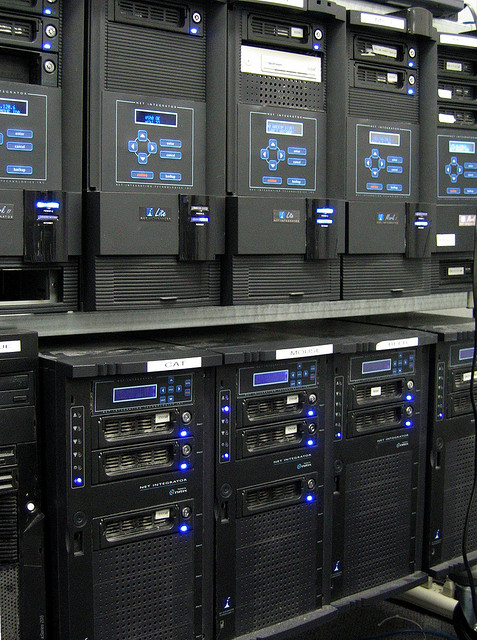
\includegraphics[width=0.48\textwidth]{images/1_02-server.jpg}}}}{servers on a rack}
\end{center}
\caption[{Tower-{}style servers on a rack. }]{Tower-{}style servers on a rack. \footnotemark{}}
\end{wrapfigure}
 \begin{DBKadmonition}{}{Note}
 
The following is written as if you are a decision maker in the early stages of conceiving a product. If you are an individual contributor in a large enterprise, or even a newcomer to an established product team, these decisions will likely have been made for you.   But at some point, \textbf{someone} had to go through this decision process, before anything could be developed.
 \end{DBKadmonition}
 
There is ferocious turbulence in the IT infrastructure market. Cloud technologies, DevOps, various platform wars\ldots{} As an entrepreneur, you need to understand what technical trends matter and what are more of same. In particular, you will need to make some level of commitment to your technical architecture. And at some point you \textbf{WILL} be asked, \textquotedblleft{}You're still using that old technology?\textquotedblright{} As a startup, you have a couple initial decisions to make regarding infrastructure and tools:
 \begin{itemize}

\item{} What is my vision for bringing my product to the world?
 

\item{} What toolset should I use to forward this vision?
 
\end{itemize}
 
As a startup, it would seem likely that you would use a commodity cloud provider. This text is based on this assumption (physical IT asset management will be discussed in Sections 3 and 4), but is there any reason why that would not work for you? The two questions are related. If you want to develop on a LAMP stack, you need a Cloud provider that will support you in this. While most are very flexible, you will need to consider the specific support levels they are offering; a provider that supports the platform (and not just the operating system) might be more valuable, but there may be higher costs and other tradeoffs. There is a near-{}infinite amount of material, debate, discussion, books, blogs, lists, and so forth concerning choice of language and platform. Exploring this area is not the purpose of this book. However, this book has certain assumptions:
 \begin{itemize}

\item{} Your system will be built, at least in part, with some form of programming language which is human-{}readable and compiled or interpreted into binary instructions.
 

\item{} Your system will run on general purpose digital computers using well known technologies.
 

\item{} Your computing environment is networked in a standard way.
 

\item{} You use the concept of a software pipeline, in which new functionality is developed in a scope distinct from what is currently offered as your product/service.
 

\item{} New functionality moves through the pipeline at significant volumes and velocity and you are concerned with optimizing this overall flow.
 
\end{itemize}
 \begin{DBKadmonition}{warning}{Important}
 
Infrastructure automation enables rapid iterations and scaling. Iterative development and rapid scaling, while possible, was often more difficult with earlier, less automated technical platforms.
 \end{DBKadmonition}
 
There is a long tradition in IT management of saying \textquotedblleft{}How can you be thinking about infrastructure before you have gone deeply into requirements?\textquotedblright{}
 
Let's be clear, in defining a product (Chapter 1) you already have started to think about requirements, although we have not yet started to use that term. The idea that all requirements need to be understood in detail before considering technical platform is, in general, an outmoded concept that made more sense when hardware was more specialized and only available as expensive, organization-{}owned assets. With the emergence of Cloud providers able to sell computing services, companies no longer need to commit to large capital outlays. And digital product professionals realize that requirements are never fully "understood" up front (more on this in the next chapter). Your Minimum Marketable Feature is an initial statement of requirements from which you should be able to infer at least initial toolset and platform requirements. Here to get you started are the major players as of this writing:
 \begin{table}[htbp]
\begin{center}
\begingroup%
\setlength{\newtblsparewidth}{\linewidth-2\tabcolsep-2\tabcolsep-2\tabcolsep-2\tabcolsep-2\tabcolsep}%
\setlength{\newtblstarfactor}{\newtblsparewidth / \real{100}}%

\begin{tabular}{llll}\hline
\multicolumn{1}{|p{25\newtblstarfactor}|}{\raggedright\bfseries%
%
Stack 1 (Enterprise Java)%
}&\multicolumn{1}{p{25\newtblstarfactor}|}{\raggedright\bfseries%
%
Stack 2 (Microsoft)%
}&\multicolumn{1}{p{25\newtblstarfactor}|}{\raggedright\bfseries%
%
Stack 3 (LAMP)%
}&\multicolumn{1}{p{25\newtblstarfactor}|}{\raggedright\bfseries%
%
Stack 4 (MEAN)%
}\tabularnewline
\cline{1-1}\cline{2-2}\cline{3-3}\cline{4-4}\multicolumn{1}{|p{25\newtblstarfactor}|}{\raggedright%
Java
%
}&\multicolumn{1}{p{25\newtblstarfactor}|}{\raggedright%
C\#
%
}&\multicolumn{1}{p{25\newtblstarfactor}|}{\raggedright%
PHP
%
}&\multicolumn{1}{p{25\newtblstarfactor}|}{\raggedright%
Javascript, Express \& Angular
%
}\tabularnewline
\cline{1-1}\cline{2-2}\cline{3-3}\cline{4-4}\multicolumn{1}{|p{25\newtblstarfactor}|}{\raggedright%
Oracle DB
%
}&\multicolumn{1}{p{25\newtblstarfactor}|}{\raggedright%
MS SQL Server
%
}&\multicolumn{1}{p{25\newtblstarfactor}|}{\raggedright%
MySQL
%
}&\multicolumn{1}{p{25\newtblstarfactor}|}{\raggedright%
MongoDB
%
}\tabularnewline
\cline{1-1}\cline{2-2}\cline{3-3}\cline{4-4}\multicolumn{1}{|p{25\newtblstarfactor}|}{\raggedright%
Websphere
%
}&\multicolumn{1}{p{25\newtblstarfactor}|}{\raggedright%
.Net
%
}&\multicolumn{1}{p{25\newtblstarfactor}|}{\raggedright%
Apache Web Server
%
}&\multicolumn{1}{p{25\newtblstarfactor}|}{\raggedright%
NodeJS
%
}\tabularnewline
\cline{1-1}\cline{2-2}\cline{3-3}\cline{4-4}\multicolumn{1}{|p{25\newtblstarfactor}|}{\raggedright%
Commercial Unix
%
}&\multicolumn{1}{p{25\newtblstarfactor}|}{\raggedright%
Microsoft Windows
%
}&\multicolumn{1}{p{25\newtblstarfactor}|}{\raggedright%
Red Hat Linux
%
}&\multicolumn{1}{p{25\newtblstarfactor}|}{\raggedright%
Ubuntu Linux
%
}\tabularnewline
\hline
\end{tabular}\endgroup%

\end{center}

\caption{Major technical stacks}
\end{table}
 
Ruby on Rails is another frequently-{}encountered platform. If you are building a data or analytics-{}centric product, there are other alternatives as well. There is a good reason, however, why you should not spend too much time \textquotedblleft{}analyzing\textquotedblright{} before you make platform decisions. The reality is that you cannot know all of the factors necessary to make a perfect decision, and in fact the way you will learn them is by moving forward and testing out various approaches. So, choose Ruby on Rails, or LAMP, or MEAN, and a hosting provider who supports them, and start. You can easily stand up environments for comparison using Cloud services, or even with lightweight virtualization on your own personal laptop. Do not fall into analysis paralysis. But \textbf{be critical of everything} especially in your first few weeks of development. Ask yourself:
 \begin{itemize}

\item{} Can I see myself doing things this way for the next year?
 

\item{} Will I be able to train people in this platform?
 

\item{} Will this scale to a bigger codebase? Higher performance? Faster throughput of new features?
 
\end{itemize}
 
If you become uncomfortable with the answers, you should consider alternatives.
 

\begin{sidebar}
\begin{DBKadmonition}{}{Tip}
 
\textbf{The technical "spike"}  Scrum-{}based development uses the concept of a \href{https://www.scrumalliance.org/community/articles/2013/march/spikes-and-the-effort-to-grief-ratio}{\textquotedblleft{}spike\textquotedblright{}} to represent effort whose outcome is not shippable product, but rather research and information. Consider thinking of your infrastructure selection process in this way.
 \end{DBKadmonition}
\end{sidebar}
 
\label{cloud}\hyperlabel{cloud}
  
\subsection{From "physical" compute to Cloud}
\label{_from_physical_compute_to_cloud}\hyperlabel{_from_physical_compute_to_cloud}%
  
According to the \href{http://csrc.nist.gov/publications/nistpubs/800-145/SP800-145.pdf}{National Institute for Standards and Technology}, Cloud is:
 

\begin{sidebar}

\emph{a model for enabling ubiquitous, convenient, on-{}demand network access to a shared pool of configurable computing resources (e.g., networks, servers, storage, applications, and services) that can be rapidly provisioned and released with minimal management effort or service provider interaction.}
\end{sidebar}
 
Before Cloud, people generally bought computers of varying sizes and power ratings to deliver the IT value they sought. With Cloud services, the same compute capacity can be rented or leased by the minute or hour, and accessed over the Internet.
 
There is much to learn about Cloud computing. In this section, we will discuss the following aspects:
 \begin{itemize}

\item{} Virtualization basics
 

\item{} Virtualization, managed services, and Cloud
 

\item{} The various kinds of Cloud services
 

\item{} Future trends
 
\end{itemize}
 
\label{virtualization}\hyperlabel{virtualization}
 
\subsubsection{Virtualization}
\label{_virtualization}\hyperlabel{_virtualization}%
  \begin{wrapfigure}{r}{0.5\textwidth}[H]

\begin{center}
\imgexists{images/1_02-laptop.jpg}{{\imgevalsize{images/1_02-laptop.jpg}{
\includegraphics[width=0.48\textwidth]{images/1_02-laptop.jpg}}}}{laptop}
\end{center}
\caption[{Laptop computer }]{Laptop computer \footnotemark{}}
\end{wrapfigure}
 
\href{https://en.wikipedia.org/wiki/Virtualization}{Virtualization}, for the purposes of this section, starts with the idea of a computer within a computer. (It has applicability to storage and networking as well but we will skip that for now.) In order to understand this, we need to understand a little bit about operating systems and how they relate to the physical computer.
 
Assume a simple, physical computer such as a laptop. When the laptop is first turned on, the operating system (OS) loads; the OS is itself software, but is able to directly control the computer's physical resources: its central processing unit (CPU), memory, screen, and any interfaces such as WiFi, USB, and Bluetooth. The operating system (in a traditional approach) then is used to run "applications" such as Web browsers, media players, word processors, spreadsheets, and the like. Many such programs can also be run as applications within the browser, but the browser still needs to be run as an application.
 \begin{wrapfigure}{r}{0.5\textwidth}[H]

\begin{center}
\imgexists{images/1_02-virt.png}{{\imgevalsize{images/1_02-virt.png}{
\includegraphics[width=0.48\textwidth]{images/1_02-virt.png}}}}{little computers inside big one}
\end{center}
\caption{Virtualization is computers within a computer}
\end{wrapfigure}
 
In the simplest form of virtualization, a specialized application known as a \emph{hypervisor} is loaded like any other application. The purpose of this hypervisor is to emulate the hardware computer in software. Once the hypervisor is running, it can emulate any number of "virtual" computers, each of which can have its own operating system. The hypervisor mediates the \href{https://en.wikipedia.org/wiki/Virtual_machine}{virtual machine} (VM) access to the actual, physical hardware of the laptop; the VM can take input from the USB port, and output to the Bluetooth interface, just like the master OS that launched when the laptop was turned on.
 \begin{DBKadmonition}{}{Tip}
 
You can experiment with a hypervisor by downloading \href{https://www.virtualbox.org/wiki/Downloads}{Virtualbox} (on Windows, Mac OS, or Linux) and using \href{https://www.vagrantup.com/}{Vagrant} to download and initialize a Linux virtual machine.   You'll probably want at least 4 gb of RAM on your laptop and a gigabyte of free disk space, at the bare minimum.
 \end{DBKadmonition}
 \begin{wrapfigure}{r}{0.5\textwidth}[H]

\begin{center}
\imgexists{images/1_02-virtualization-types.png}{{\imgevalsize{images/1_02-virtualization-types.png}{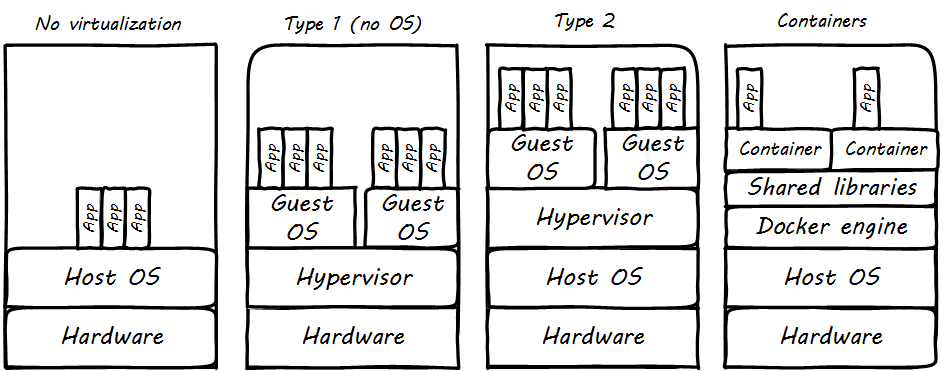
\includegraphics[width=0.48\textwidth]{images/1_02-virtualization-types.png}}}}{Virtualization types}
\end{center}
\caption{Virtualization types}
\end{wrapfigure}
 
There are two different kinds of hypervisors. The example we just discussed was an example of a Type 2 hypervisor, which runs on top of a host operating system. In a Type 1 hypervisor, a master host OS is not used; the hypervisor runs on the "bare metal" of the computer and in turn "hosts" multiple VMs.
 
\label{containers}\hyperlabel{containers}
 \begin{wrapfigure}{r}{0.5\textwidth}[H]

\begin{center}
\imgexists{images/1_02-containers.png}{{\imgevalsize{images/1_02-containers.png}{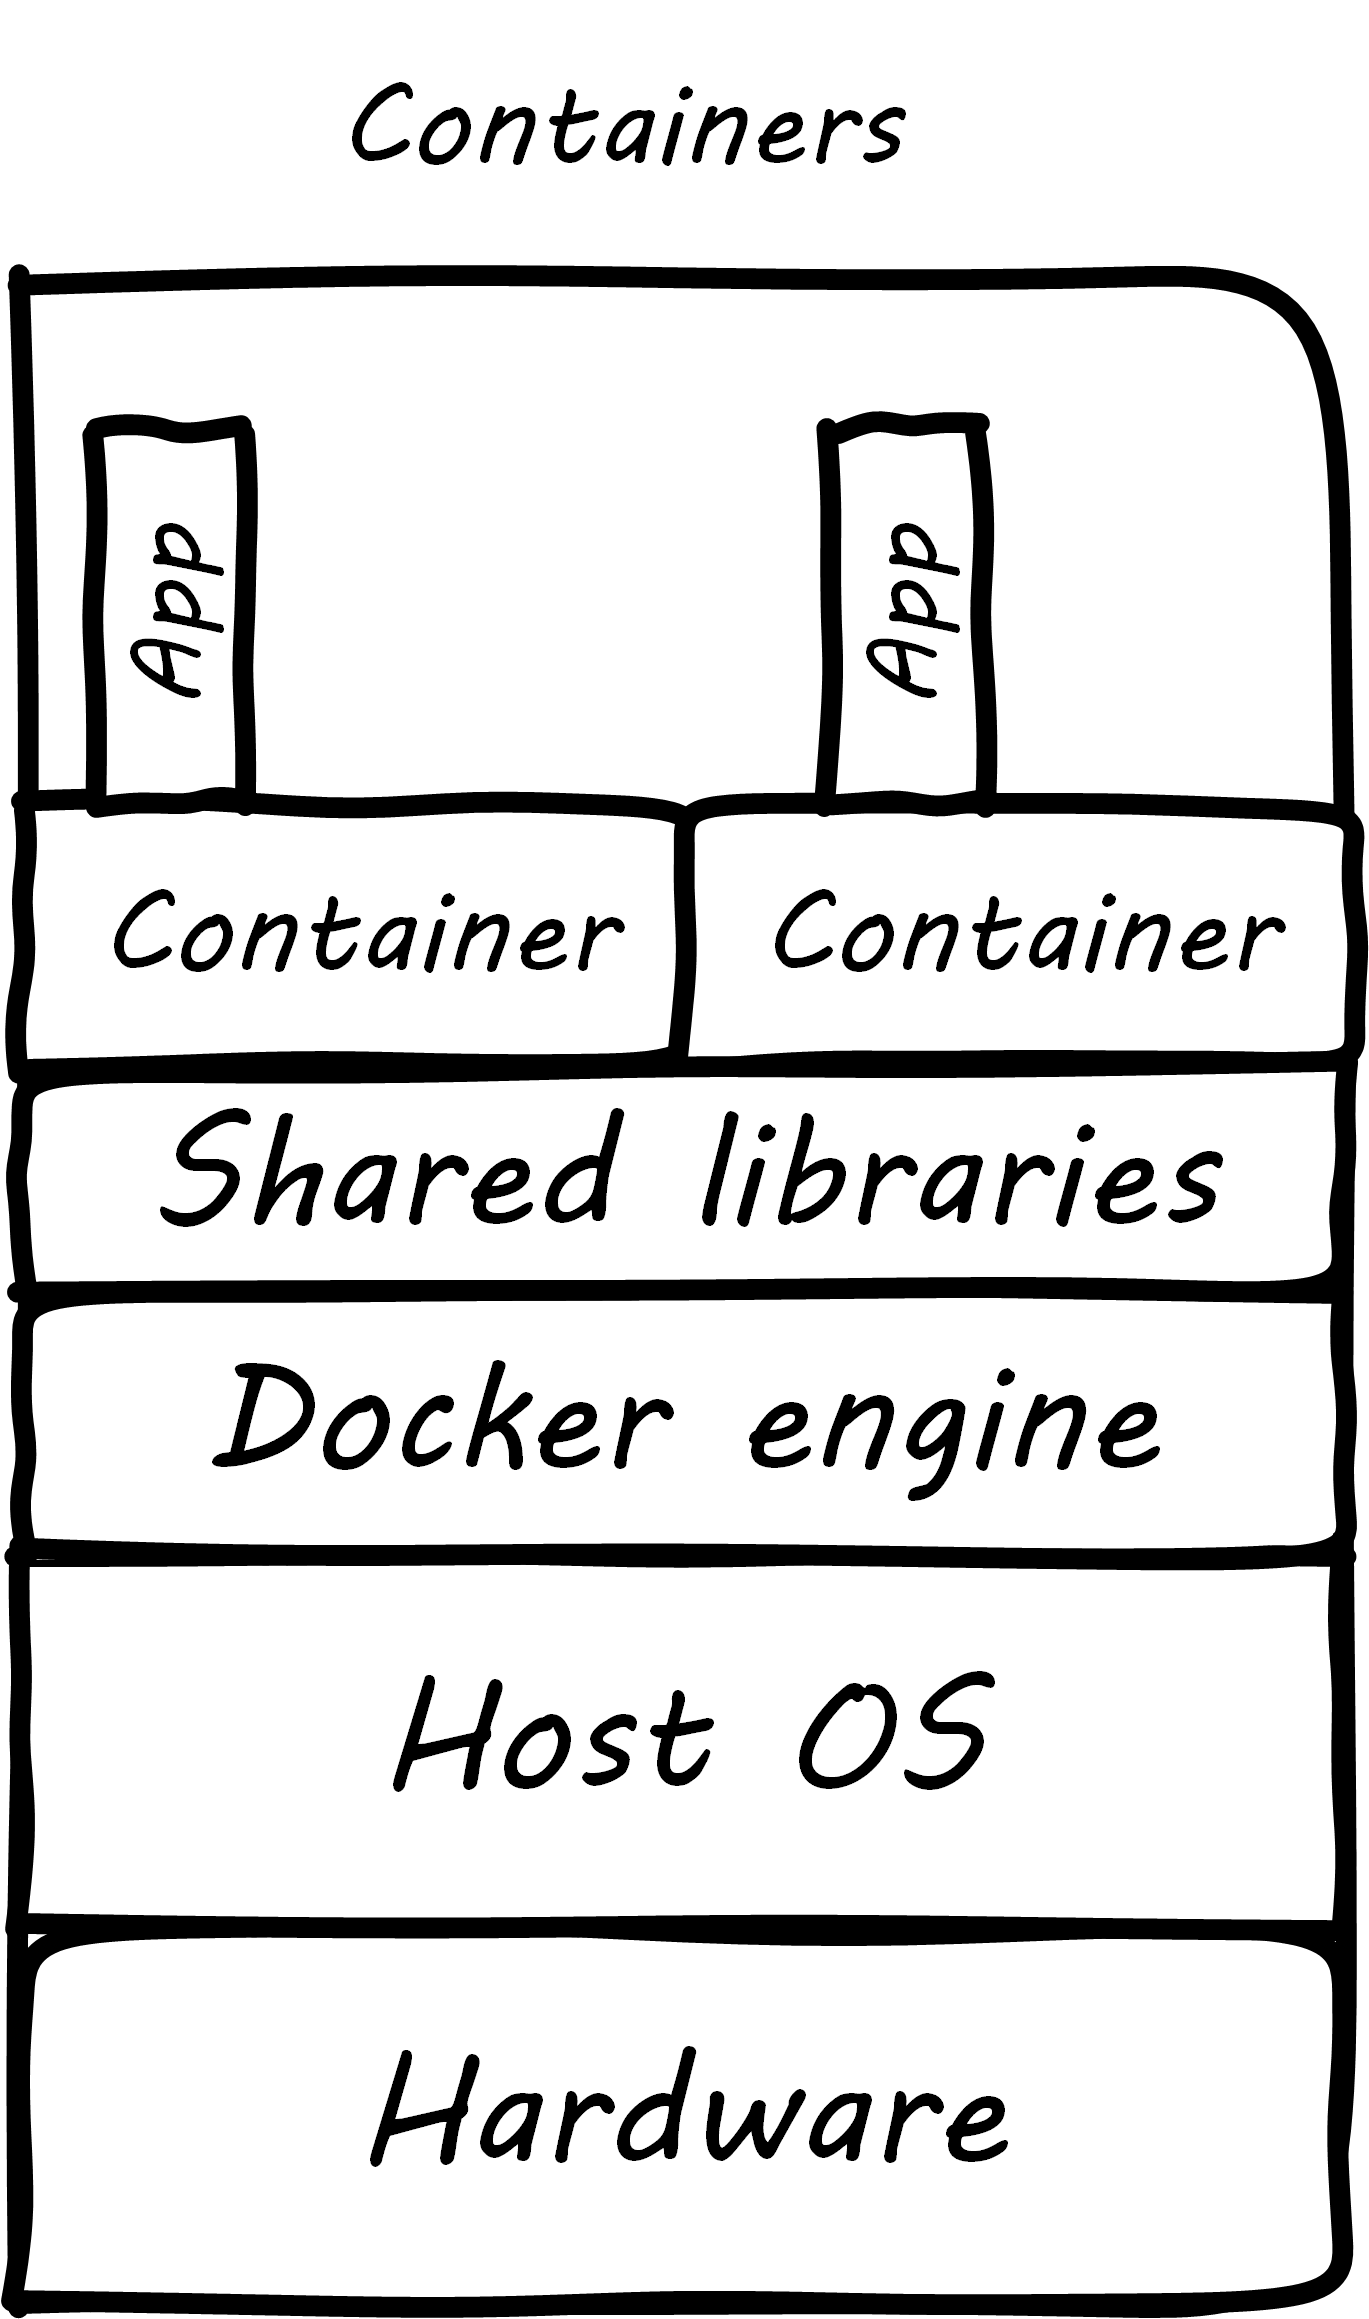
\includegraphics[width=0.48\textwidth]{images/1_02-containers.png}}}}{containers}
\end{center}
\caption{Containers}
\end{wrapfigure}
 
\emph{Paravirtualization}, e.g. containers, is another form of virtualization found in the marketplace. In a paravirtualized environment, a core operating system is able to abstract hardware resources for multiple virtual guest environments without having to virtualize hardware for each guest. The benefit of this type of virtualization is increased input/output (I/O) efficiency and performance for each of the guest environments.
 
However, while hypervisors can support a diverse array of virtual machines with different operating systems on a single computing node, guest environments in a paravirtualized system generally share a single OS.
 \begin{DBKadmonition}{}{Note}
 
Virtualization was predicted in the earliest theories that led to the development of computers. Turing and Church realized that any general purpose computer could emulate any other. Virtual systems have existed in some form since \href{https://en.wikipedia.org/wiki/Timeline_of_virtualization_development}{at latest 1967} -{} only 20 years after the first fully functional computers.  And yes, you can run computers within computers within computers with virtualization. They get slower and slower the more levels you go in, but the logic still works.
 \end{DBKadmonition}
 
\label{virtualization-econ}\hyperlabel{virtualization-econ}
  
\subsubsection{Why is virtualization important?}
\label{_why_is_virtualization_important}\hyperlabel{_why_is_virtualization_important}%
  
Virtualization attracted business attention as a means to consolidate computing workloads. For years, companies would purchase servers to run applications of various sizes, and in many cases the computers were badly underutilized. Because of configuration issues (legitimate) and an overabundance of caution (questionable), average utilization in a pre-{}virtualization data center might average 10-{}20\%. (That's 90\% of the computer's capacity being wasted.)
 \begin{wrapfigure}{r}{0.5\textwidth}[H]

\begin{center}
\imgexists{images/1_02-physUtil.png}{{\imgevalsize{images/1_02-physUtil.png}{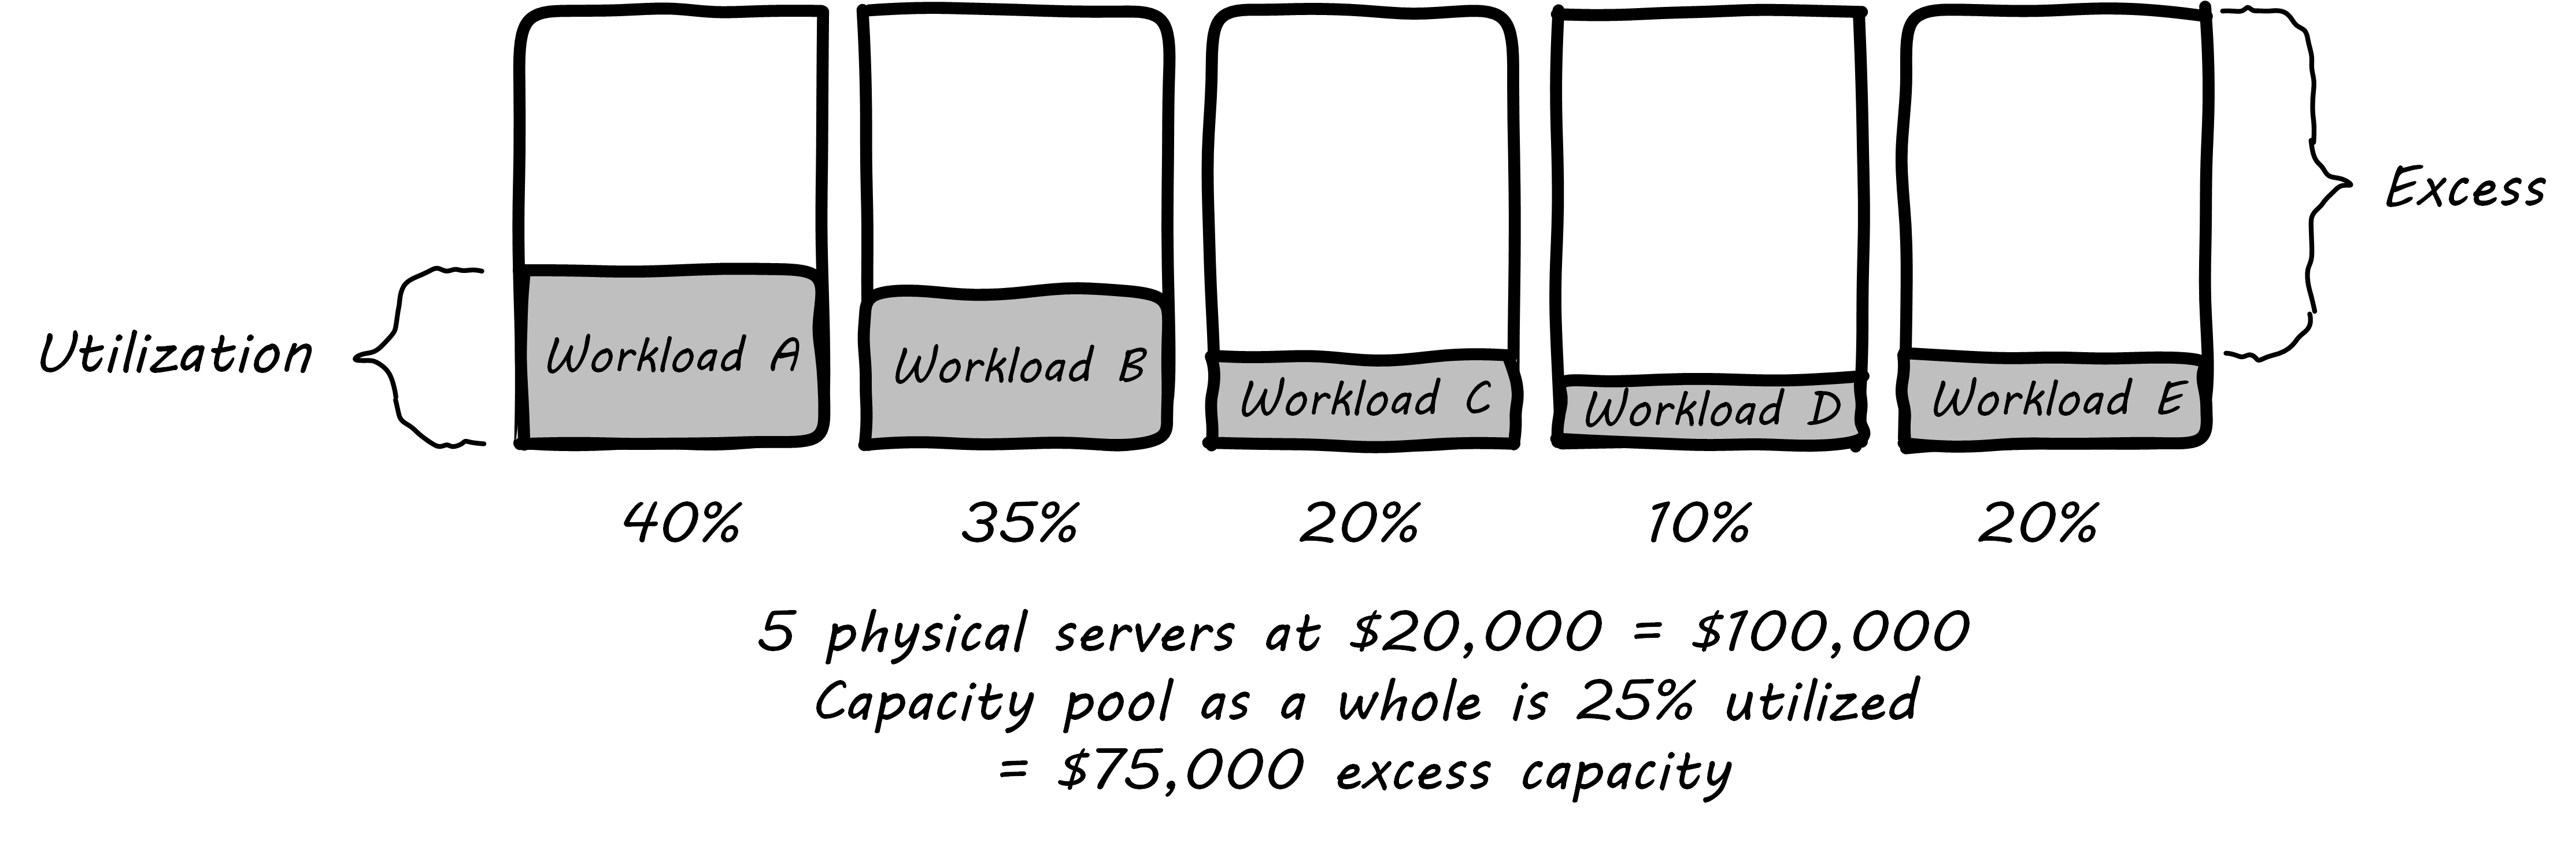
\includegraphics[width=0.48\textwidth]{images/1_02-physUtil.png}}}}{underutilization}
\end{center}
\caption{Inefficient utilization}
\end{wrapfigure}
 
The above figure is a simplification. Computing and storage infrastructure supporting each application stack in the business were sized to support each workload. For example, a payroll server might run on a different infrastructure configuration than a data warehouse server. Large enterprises needed to support hundreds of different infrastructure configurations, increasing maintenance and support costs.
 
The adoption of virtualization allowed businesses to compress multiple application workloads onto a smaller number of physical servers:
 \begin{wrapfigure}{r}{0.5\textwidth}[H]

\begin{center}
\imgexists{images/1_02-virtUtil.png}{{\imgevalsize{images/1_02-virtUtil.png}{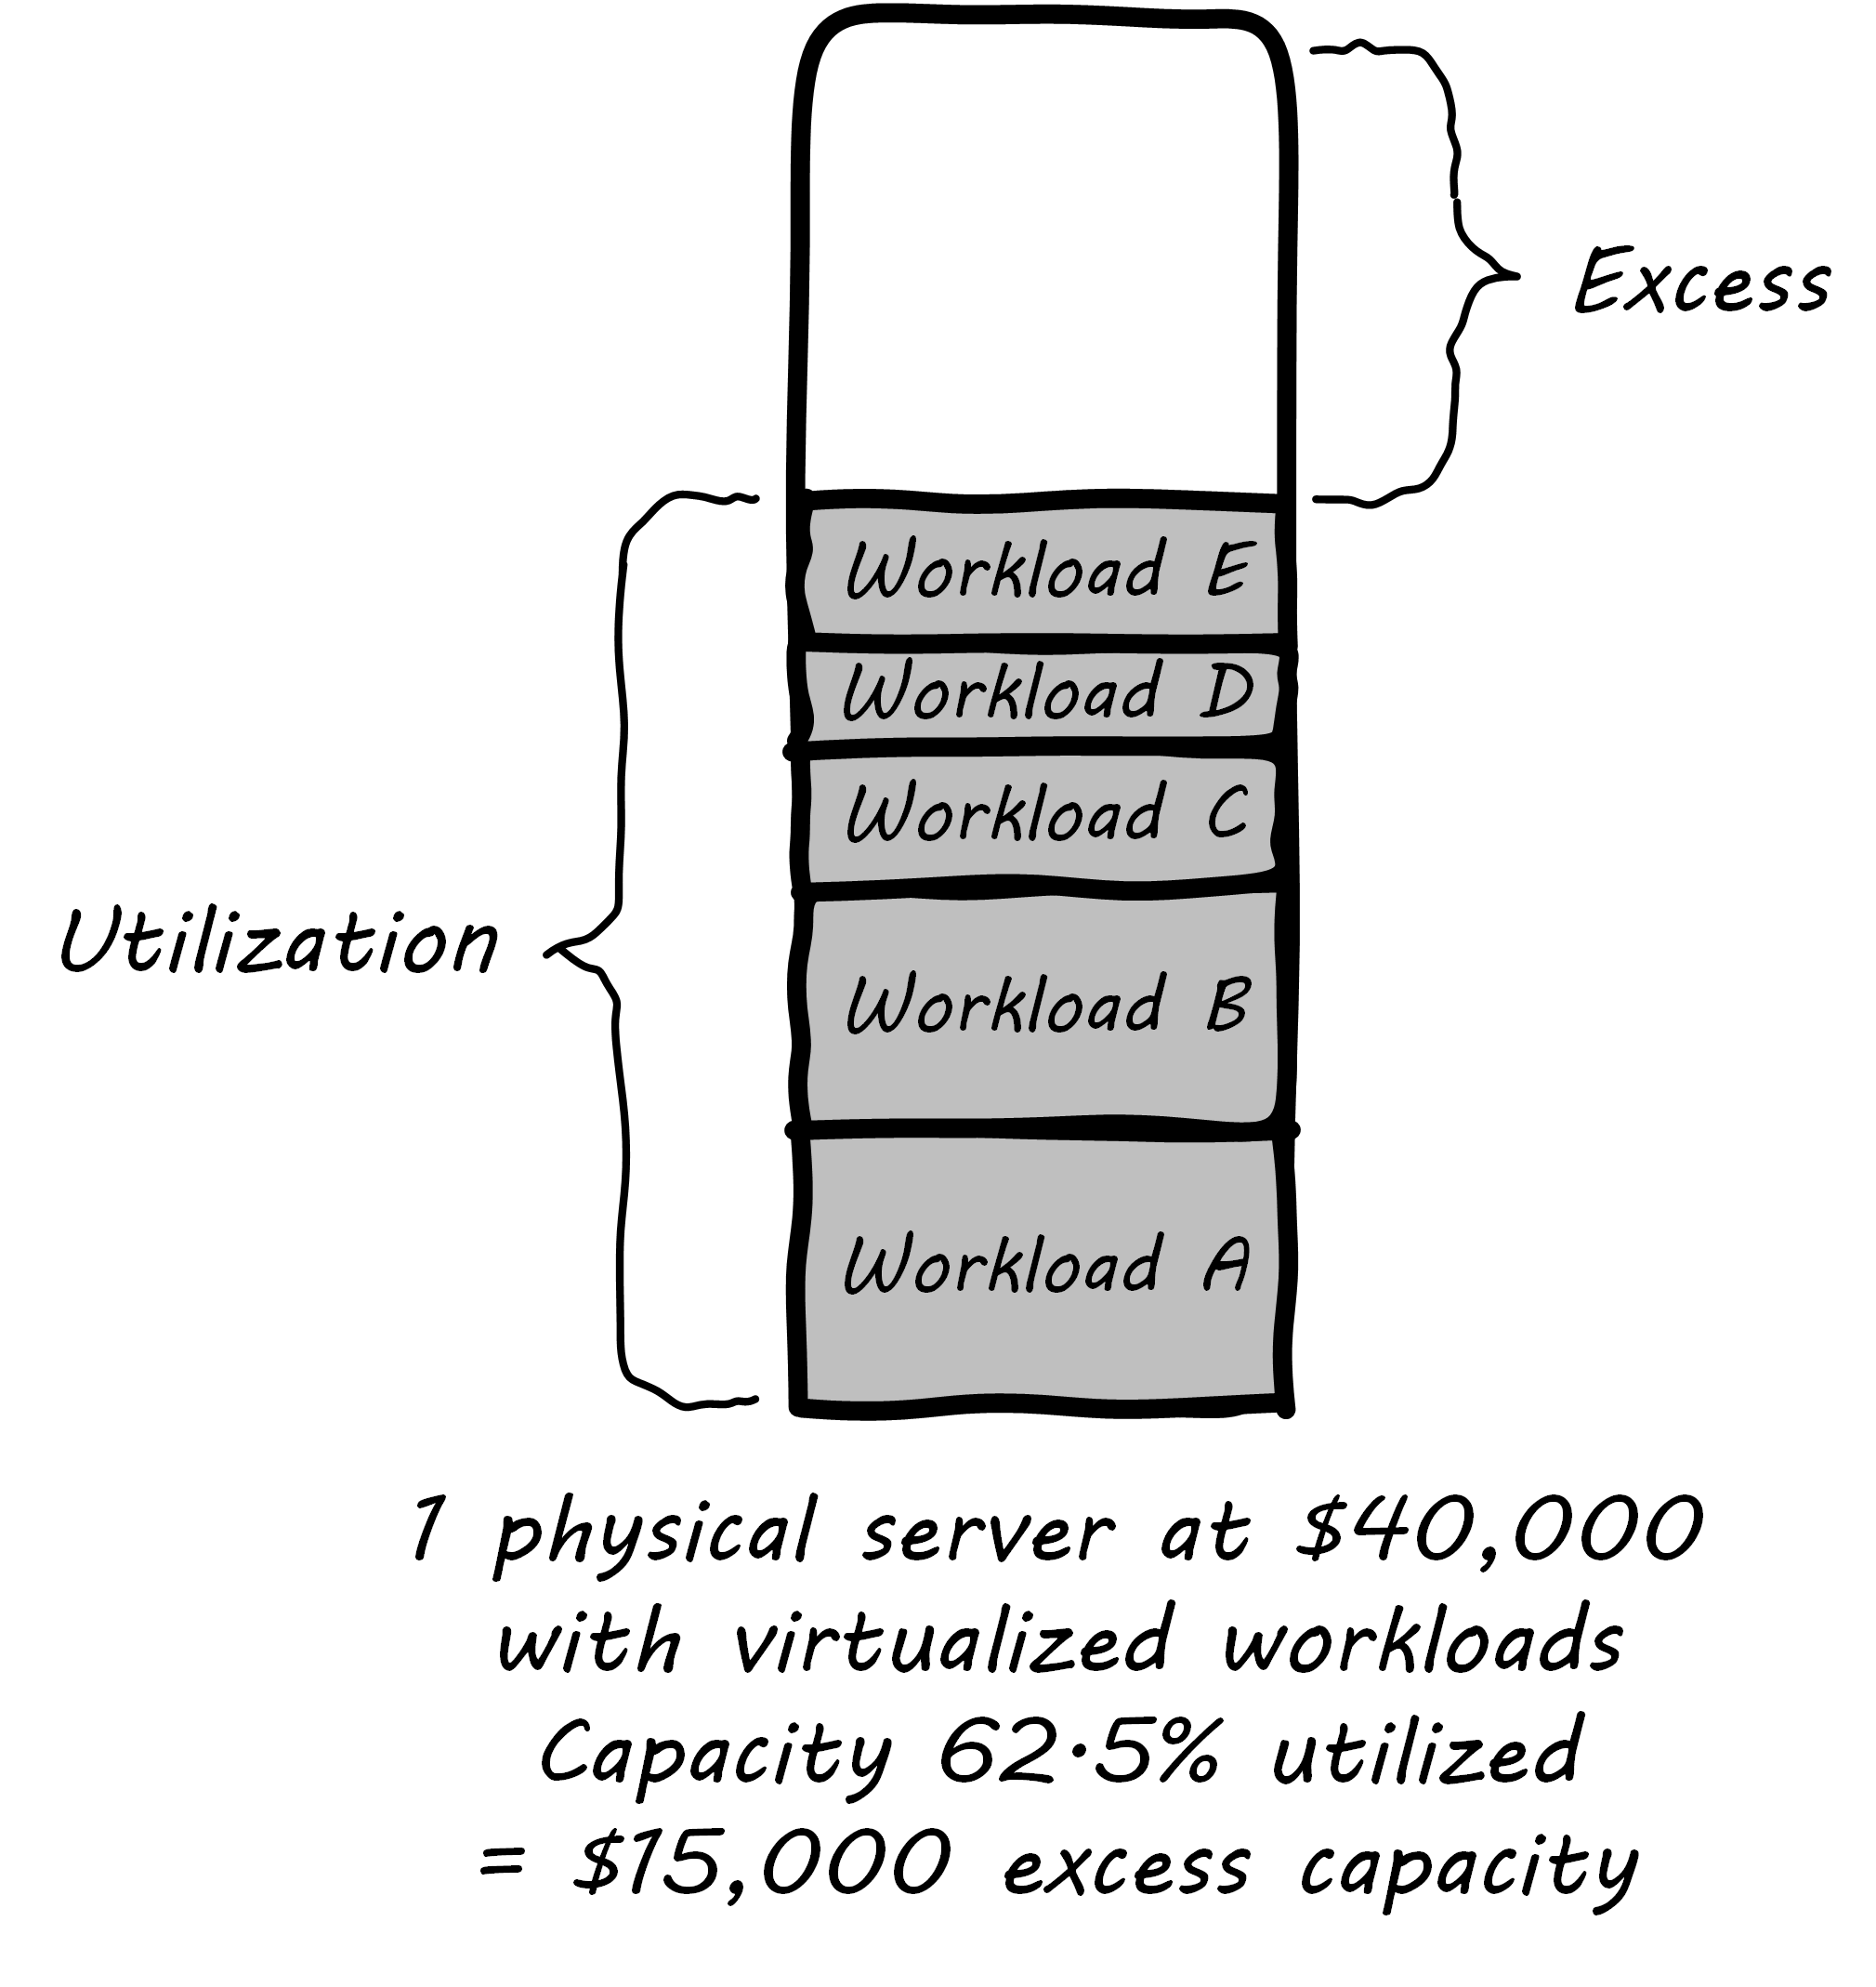
\includegraphics[width=0.48\textwidth]{images/1_02-virtUtil.png}}}}{efficient util}
\end{center}
\caption{Efficiency through virtualization}
\end{wrapfigure}
 \begin{DBKadmonition}{}{Note}
 
For illustration only. A utilization of 62.5\% might actually be a bit too high for comfort, depending on the variability and criticality of the workloads.
 \end{DBKadmonition}
 
In most virtualized architectures, the physical servers supporting workloads share a consistent configuration, which made it easy to add and remove resources from the environment. The virtual machines may still vary greatly in configuration, but the fact of virtualization makes managing that easier -{} the virtual machines can be easily copied and moved, and increasingly can be defined as a form of code (see next section).
 
Virtualization thus introduced a new design pattern into the enterprise where computing and storage infrastructure became commoditized building blocks supporting an ever-{}increasing array of services. But what about where the application is large and virtualization is mostly overhead? Virtualization still may make sense in terms of management consistency and ease of system recovery.
  
\subsubsection{Virtualization, managed services, and cloud}
\label{_virtualization_managed_services_and_cloud}\hyperlabel{_virtualization_managed_services_and_cloud}%
  
Companies have always sought alternatives to owning their own computers.  is a long tradition of managed services, where applications are built out by a customer and then their management is outsourced to a third party. Using fractions of mainframe "time-{}sharing" systems is a practice that dates back decades. However, such relationships took effort to set up and manage, and might even require bringing physical tapes to the third party (sometimes called a "service bureau.") Fixed price commitments were usually high (the customer had to guarantee to spend X dollars.) Such relationships left much to be desired in terms of  responsiveness to change.
 
As computers became cheaper, companies increasingly acquired their own data centers, investing large amounts of capital in high-{}technology spaces with extensive power and cooling infrastructure. This was the trend through the late 1980s to about 2010, when Cloud computing started to provide a realistic alternative with true "pay as you go" pricing, analogous to electric metering.
 \begin{wrapfigure}{r}{0.5\textwidth}[H]

\begin{center}
\imgexists{images/1_02-parkhill.png}{{\imgevalsize{images/1_02-parkhill.png}{
\includegraphics[width=0.48\textwidth]{images/1_02-parkhill.png}}}}{book}
\end{center}
\caption{Cloud computing started here}
\end{wrapfigure}
 
The idea of running IT completely as a utility service goes back at least to 1965 and the publication of \emph{The Challenge of the Computer Utility}, by Douglas Parkhill. While the conceptual idea of Cloud and utility computing was foreseeable fifty years ago, it took many years of hard-{}won IT evolution to support the vision. Reliable hardware of exponentially increasing performance, robust open-{}source software, Internet backbones of massive speed and capacity, and many other factors converged towards this end.
 
However, people store data -{} often private -{} on computers. In order to deliver compute as a utility, it is essential to segregate each customer's workload from all others. This is called \emph{multi-{}tenancy}. In multi-{}tenancy, multiple customers share physical resources that provide the illusion of being dedicated.
 \begin{DBKadmonition}{}{Note}
 
The phone system has been multi-{}tenant ever since they got rid of \href{https://en.wikipedia.org/wiki/Party_line_(telephony)}{party lines}. A party line was a shared line where anyone on it could hear every other person.
 \end{DBKadmonition}
 
In order to run compute as a utility, multi-{}tenancy was essential. This is different from electricity (but similar to the phone system). As noted elsewhere, one watt of electric power is like any other and there is less concern for leakage or unexpected interactions. People's bank balances are not encoded somehow into the power generation and distribution infrastructure.
 
Virtualization is necessary, but not sufficient for cloud. True Cloud services are highly automated, and most Cloud analysts will insist that if virtual machines cannot be created and configured in a completely automated fashion, the service is not true Cloud. This is currently where many in-{}house "private" Cloud efforts struggle; they may have virtualization, but struggle to make it fully self-{}service.
 
\label{cloud-models}\hyperlabel{cloud-models}
 
Cloud services have refined into at least three major models:
 \begin{itemize}

\item{} Infrastructure as a service
 

\item{} Platform as a service
 

\item{} Software as a service
 
\end{itemize}
 

\begin{sidebar}

\textbf{From the \href{http://csrc.nist.gov/publications/nistpubs/800-145/SP800-145.pdf}{NIST Definition of Cloud Computing (p. 2-{}3)}:}

\textbf{Software as a Service (SaaS).} The capability provided to the consumer is to use the provider's applications running on a cloud infrastructure. The applications are accessible from various client devices through either a thin client interface, such as a web browser (e.g., web-{}based email), or a program interface. The consumer does not manage or control the underlying cloud infrastructure including network, servers, operating systems, storage, or even individual application capabilities, with the possible exception of limited user-{}specific application configuration settings.

\textbf{Platform as a Service (PaaS).} The capability provided to the consumer is to deploy onto the cloud infrastructure consumer-{}created or acquired applications created using programming languages, libraries, services, and tools supported by the provider. The consumer does
not manage or control the underlying cloud infrastructure including network, servers, operating systems, or storage, but has control over the deployed applications and possibly configuration settings for the application-{}hosting environment.

\textbf{Infrastructure as a Service (IaaS).} The capability provided to the consumer is to provision processing, storage, networks, and other fundamental computing resources where the consumer is able to deploy and run arbitrary software, which can include operating systems and applications. The consumer does not manage or control the underlying cloud infrastructure but has control over operating systems, storage, and deployed applications; and possibly limited control of select networking components (e.g., host firewalls).
\end{sidebar}
 
There are Cloud services beyond those listed above (e.g. Storage as a Service). Various platform services have become extensive on providers such as Amazon, which offers load balancing, development pipelines, various kinds of storage, and much more.
 \begin{DBKadmonition}{}{Note}
 
Traditional managed services are sometimes called "your mess for less." With Cloud, you have to "clean it up first."
 \end{DBKadmonition}
  
\subsubsection{Containers and looking ahead}
\label{_containers_and_looking_ahead}\hyperlabel{_containers_and_looking_ahead}%
  
At this writing, two major developments in Cloud computing are prominent:
 \begin{itemize}

\item{} The combination of Cloud computing with paravirtualization, including technologies such as \href{http://www.zdnet.com/article/what-is-docker-and-why-is-it-so-darn-popular/}{Docker}
 \begin{itemize}

\item{} Containers are lighter weight than virtual machines
 \begin{itemize}

\item{} Virtualized Guest OS: Seconds to instantiate
 

\item{} Container: Milliseconds (!)
 
\end{itemize}
 

\item{} Containers must be the same OS as host
 
\end{itemize}
 

\item{} \href{https://aws.amazon.com/lambda/}{AWS Lambda}, "a compute service that runs your code in response to events and automatically manages the compute resources for you, making it easy to build applications that respond quickly to new information."
 
\end{itemize}
 
It's recommended you at least scan the links provided.
 
\label{scale-matters}\hyperlabel{scale-matters}
 

\begin{sidebar}
\begin{DBKadmonition}{warning}{Important}
 
Eventually, scale matters. As your IT service's usage increases, you will inevitably find that you need to start caring about technical details such as storage and network architecture. The implementation decisions made by you and your service providers may become inefficient for the particular "workload" your product represents, and you will need to start asking questions. The brief technical writeup, \href{https://gist.github.com/jboner/2841832}{Latency Numbers Every Programmer Should Know} can help you start thinking about these issues.
 \end{DBKadmonition}
\end{sidebar}
 
\label{infracode}\hyperlabel{infracode}
   
\subsection{Infrastructure as code}
\label{_infrastructure_as_code}\hyperlabel{_infrastructure_as_code}%
  \begin{quote}

Infrastructure as code is an approach to infrastructure automation based on practices from software development. It emphasizes consistent, repeatable routines for provisioning and changing systems and their configuration. Changes are made to definitions and then rolled out to systems through unattended processes that include thorough validation. The premise is that modern tooling can treat infrastructure as if it were software and data. This allows people to apply software development tools such as version control systems (VCS), automated testing libraries, and deployment orchestration to manage infrastructure. It also opens the door to exploit development practices such as test-{}driven development (TDD), continuous integration (CI), and continuous delivery (CD).

\hspace*\fill--- Kief Morris
\emph{Infrastructure as Code: Managing Servers in the Cloud} \end{quote}
 
So, what is infrastructure as code?
 
As cloud infrastructures have scaled, there has been an increasing need to configure many servers identically. Auto-{}scaling (adding more servers in response to increasing load) has become a widely used strategy as well. Both call for increased automation in the provisioning of IT infrastructure. It is simply not possible for a human being to be hands on at all times in configuring and enabling such infrastructures, so automation is called for.
 
In years past, infrastructure administrators relied on ad-{}hoc issuance of commands either at an operations console, or via a GUI-{}based application. Shell scripts might be used for various repetitive processes, but administrators by tradition and culture were empowered to issue arbitrary commands to alter the state of the running system directly.
 
The following passage from The Phoenix Project captures some of the issues. The speaker is Wes, the infrastructure manager, who is discussing a troubleshooting scenario:
 
\emph{\textquotedblleft{}Several months ago, we were three hours into a Sev 1 outage, and we bent over backward not to escalate to Brent. But eventually, we got to a point where we were just out of ideas, and we were starting to make things worse. So, we put Brent on the problem.\textquotedblright{} He shakes his head, recalling the memory, \textquotedblleft{}He sat down at the keyboard, and it's like he went into this trance. Ten minutes later, the problem is fixed. Everyone is happy and relieved that the system came back up. But then someone asked, `How did you do it?' And I swear to God, Brent just looked back at him blankly and said, `I have no idea. I just did it.'\textquotedblright{}}
 
\hyperlink{Kim2013}{[Kim2013]}, p. 116.
 
Obviously, \textquotedblleft{}close your eyes and go into a trance\textquotedblright{} is not a repeatable process. It is not a procedure or operation that can be archived and distributed across multiple servers. So, shell scripts or more advanced forms of automation are written and increasingly, all actual server configuration is based on such pre-{}developed specification. It is becoming more and more rare for a systems administrator to actually \textquotedblleft{}log in\textquotedblright{} to a server and execute configuration-{}changing commands in an ad-{}hoc manner (as Brent).
 
In fact, because virtualization is becoming so powerful, servers increasingly are destroyed and rebuilt at the first sign of any trouble. In this way, it is certain that the server's configuration is as intended. This again is a relatively new practice.
 
Previously, because of the expense and complexity of bare-{}metal servers, and the cost of having them offline, great pains were taken to fix troubled servers. Systems administrators would spend hours or days troubleshooting obscure configuration problems, such as residual settings left by removed software. Certain servers might start to develop \textquotedblleft{}personalities.\textquotedblright{} Industry practice has changed dramatically here since around 2010.
 
\label{infra-code-example}\hyperlabel{infra-code-example}
 
\subsubsection{A simple infrastructure as code example}
\label{_a_simple_infrastructure_as_code_example}\hyperlabel{_a_simple_infrastructure_as_code_example}%
  
\textbf{Note, the below Part Is illustrative only, and is not intended as a lab. The associated lab for this book goes into depth on these topics.}
 
In presenting infrastructure as code at its simplest, we will start with the concept of a shell script. While this is not a deep Linux book (there are many others out there, starting with the excellent O'Reilly lineup), some basic technical literacy is assumed in this book. Consider the following set of commands:
 
\begin{lstlisting}[firstnumber=1,backgroundcolor={},basicstyle=\ttfamily,]
$ mkdir foo bar
$ cd foo
$ touch x y z
$ cd ../bar
$ touch a b c
\end{lstlisting}
 
What does this do? It tells the computer:
 \begin{enumerate}[label=\arabic*.]

\item{} Create (\texttt{mkdir}) two directories, one named foo and one named bar.
 

\item{} Move (\texttt{cd}) to the one named foo
 

\item{} Create (\texttt{touch}) three files, named x, y, and z
 

\item{} Move to the directory named bar
 

\item{} Create three blank files, named a, b, and c.
 
\end{enumerate}
 
If you find yourself (with the appropriate permissions) at a Unix command prompt, and run those commands, you will wind up with a configuration that could be visualized as this:
 \begin{wrapfigure}{r}{0.5\textwidth}[H]

\begin{center}
\imgexists{images/1_02-iac.png}{{\imgevalsize{images/1_02-iac.png}{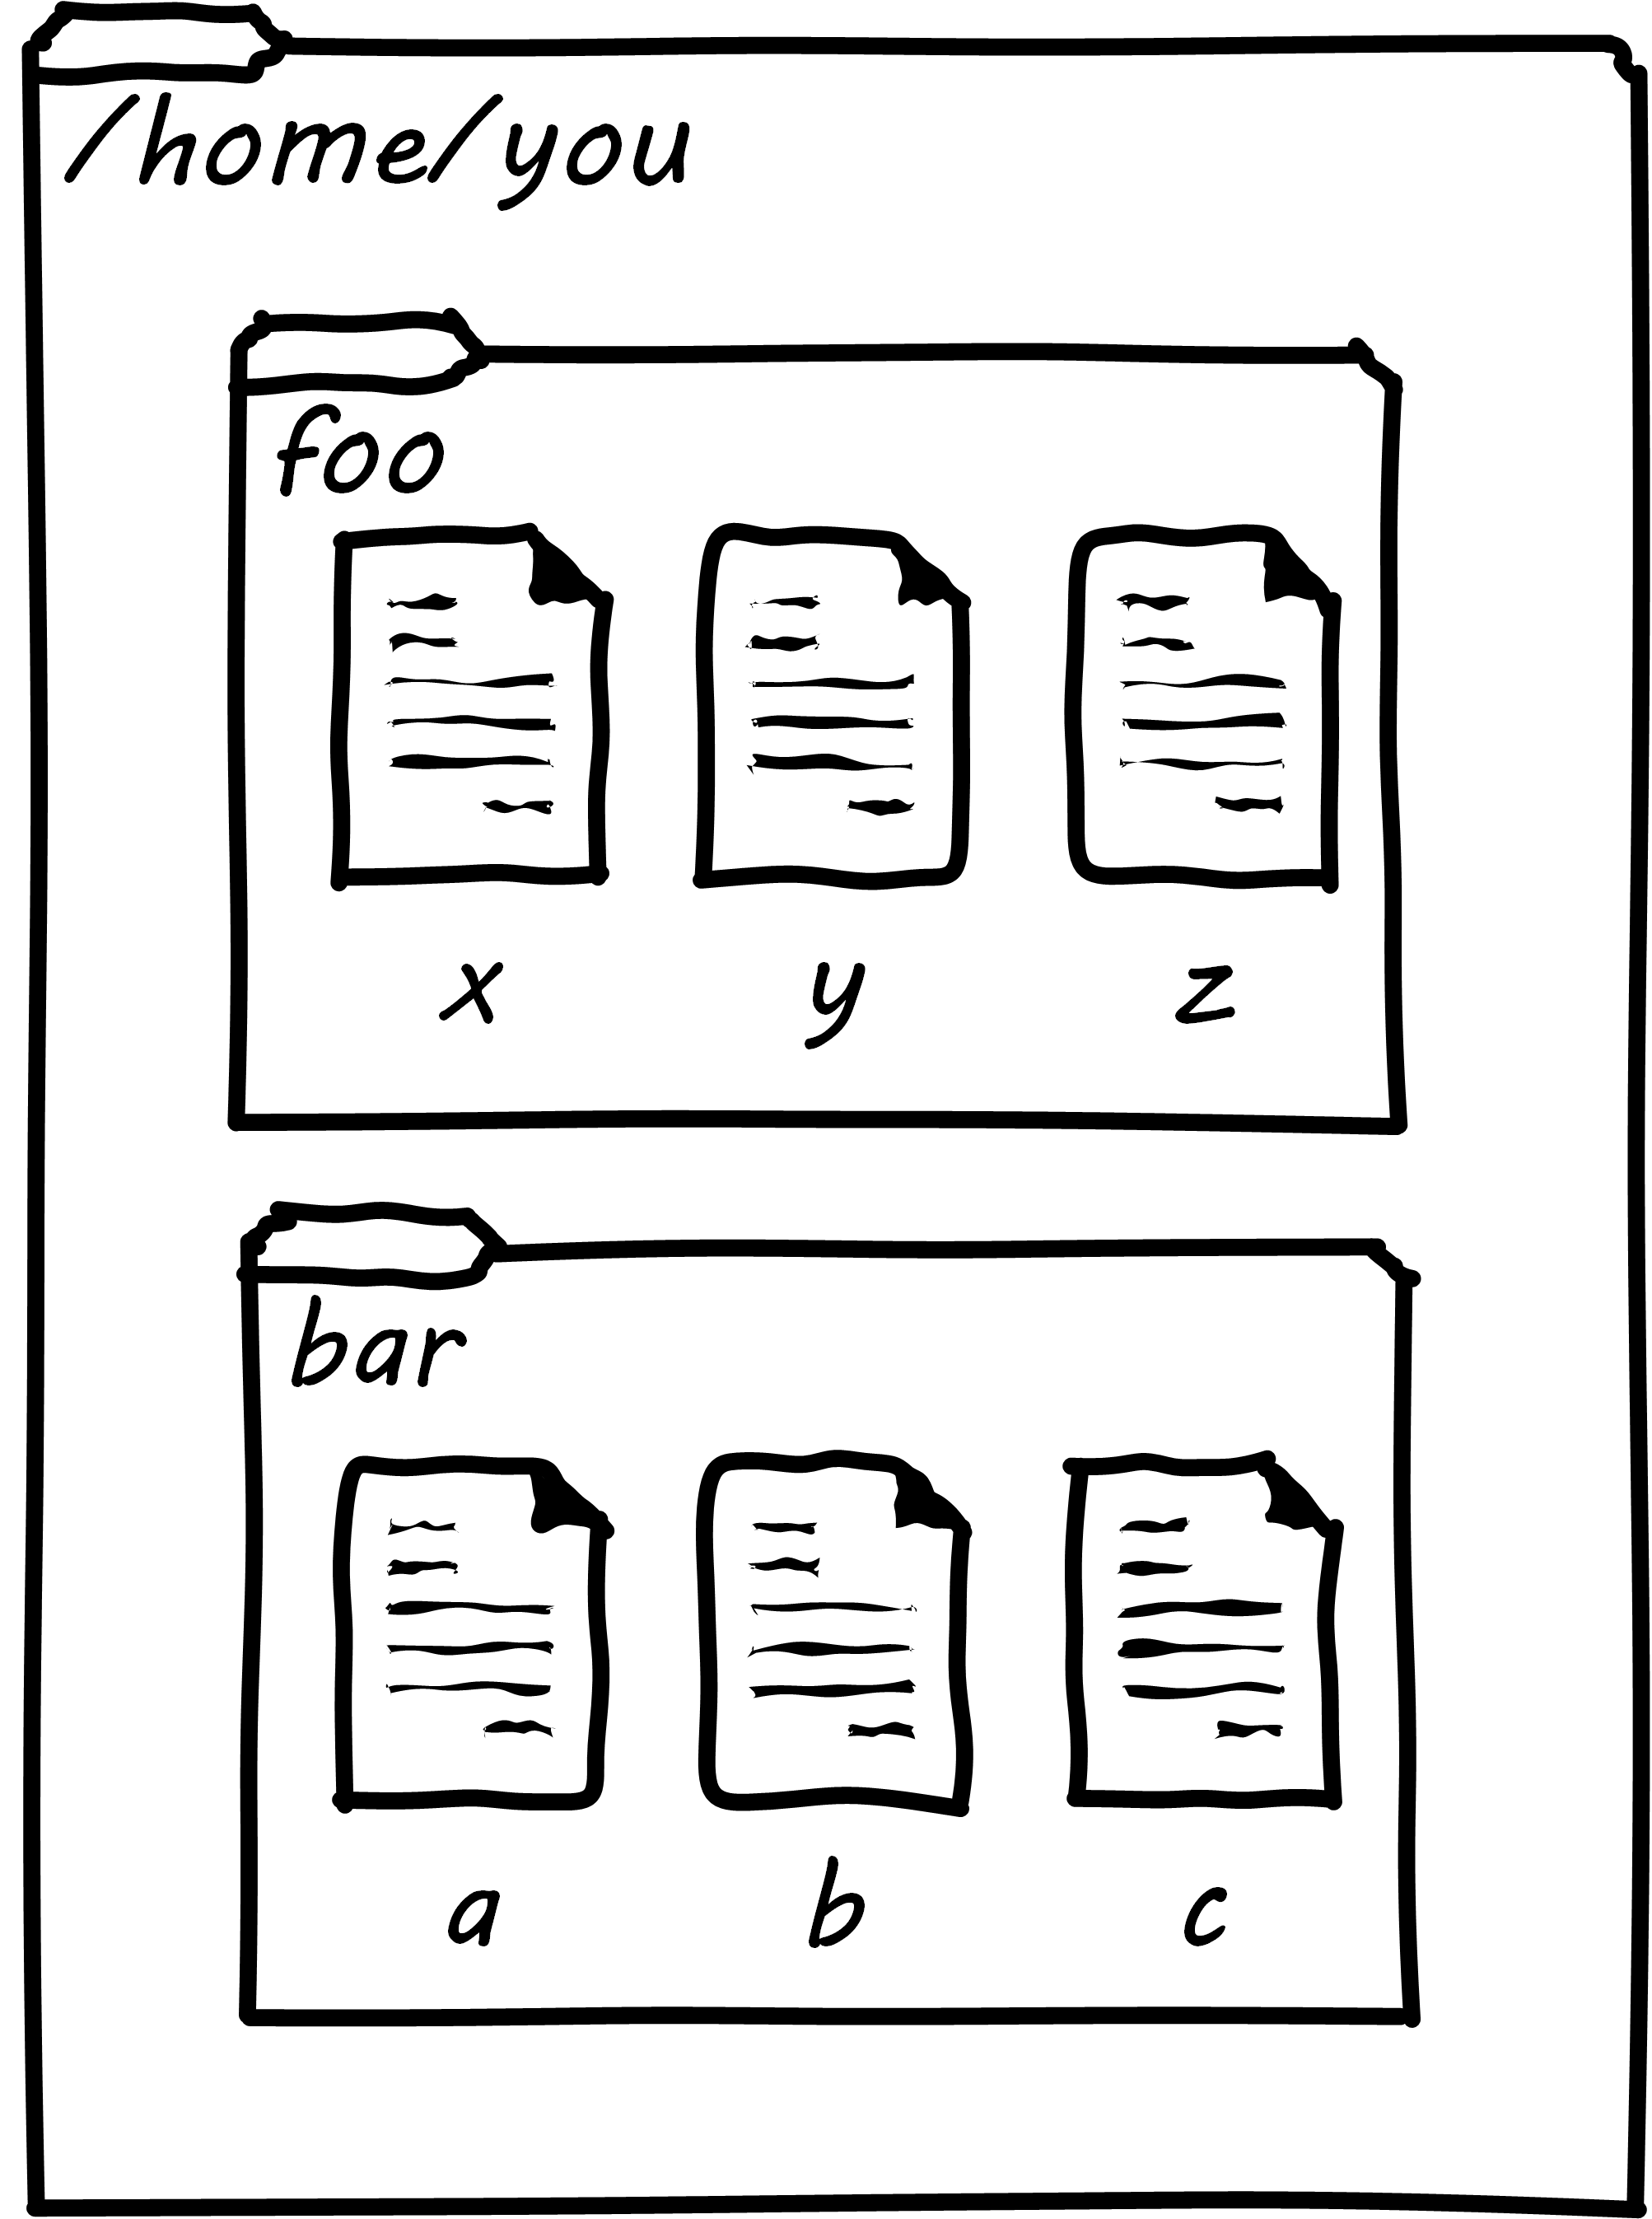
\includegraphics[width=0.48\textwidth]{images/1_02-iac.png}}}}{folders/files}
\end{center}
\caption{Simple directory/file structure}
\end{wrapfigure}
 
(If you don't understand this, you should probably spend a couple hours with a Linux tutorial).
 
Configuration, you ask? Something this trivial? Yes, directory and file layouts count as configuration and in some cases are critical. Now, what if we take that same set of commands, and put them in a file thus:
 
\begin{lstlisting}[firstnumber=1,backgroundcolor={},basicstyle=\ttfamily,]
#!/bin/bash
mkdir foo bar
cd foo
touch x y z
cd ../bar
touch a b c
\end{lstlisting}
 
We might name that file \texttt{iac.\penalty0 sh}, set its permissions correctly, and run it (so that the computer executes all the commands for us, rather than us running them one at a time at the console).  If we did so in an empty directory, we'd again wind up with that same configuration. (If we did it in a directory already containing foo and bar directories, we'd get errors. More on this to come.)
 \begin{DBKadmonition}{}{Note}
 
The state of the art in infrastructure configuration is not to use shell scripts at all but rather policy-{}based infrastructure management approaches, which we discuss subsequently.
 \end{DBKadmonition}
 
This will be familiar material to many of you, including the fact that beyond creating directories and files we can use shell scripts to create and destroy virtual servers, install and remove software, set up and delete users, check on the status of running processes, and much more.
 
Sophisticated infrastructure as code techniques are are essential part of modern site reliability engineering practices such as used by Google. Auto-{}scaling, self-{}healing systems, fast deployments of new features all require that infrastructure be represented as code for maximum speed and reliability of creation.
 
Let's return to our iac.sh file. It's valuable. It documents our intentions for how this configuration should look. We can reliably run it on thousands of machines and it will always give us two directories and six files. In terms of the previous section, we might choose to run it on every new server we create. We want to establish it as a known resource in our technical ecosystem. This is where version control and the broader concept of configuration management come in.
 

\begin{sidebar}
\textbf{Cattle not pets?}


In earlier times, servers (that is, computers managed on a distributed network) were usually configured without virtualization. They arrived (carefully packed on pallets) from the manufacturer unconfigured, and would be painstakingly "built" by the systems administrator: the operating system would be compiled and installed, key software packages (such as Java) installed, and then the organization's customer software installed.

At best, the systems administrators, or server engineers, might have written guidelines or perhaps some shell scripts that would be run on the server to configure it in a semi-{}consistent way. But that documentation would often be out of date, the scripts would be unique to a given administrator, and there would be great reluctance to "rebuild the box" -{} that is, to delete everything on it and do a "clean re-{}install." Instead, if there were problems, the administrator would try to fix the server by going in and adjusting particular settings (typically by changing configuration files and restarting services), or deleting software packages and re-{}installing them.

The problem with this is that modern computing systems are so complex that deleting software can be difficult; if the un-{}install process fails in some way, the server can be left in a compromised state. Similarly, one-{}time configuration adjustments made to one server means that it may be inconsistent with similar devices, and this can cause problems. For example, if the first systems administrator is on vacation, their substitute may expect the server to be configured in a certain way and make adjustments that have unexpected effects. Or the first systems administrator themselves may forget exactly what it is they did. Through such practices, servers would start to develop personalities, because their configurations were inconsistent.

As people started to work more and more with virtualization, they realized it was easier to rebuild virtual servers from scratch, rather than trying to fix them. Automated configuration management tools helped by promoting a consistent process for rebuilding. Randy Bias, noting this, put forth the provocative idea that "servers are cattle, not pets" \hyperlink{Bias2012}{[Bias2012]}. That is, when a pet is sick, one takes it to the vet, but a sick cow might simply  be taken out and shot.

I prefer the saying that "servers are fleet vehicles, not collectible cars" as it seems less cruel, and the cattle metaphor overlooks the fact that large animal veterinarians are routinely employed in the cattle industry.
\begin{wrapfigure}{r}{0.5\textwidth}[H]

\begin{center}
\imgexists{images/1_02-vehicles.png}{{\imgevalsize{images/1_02-vehicles.png}{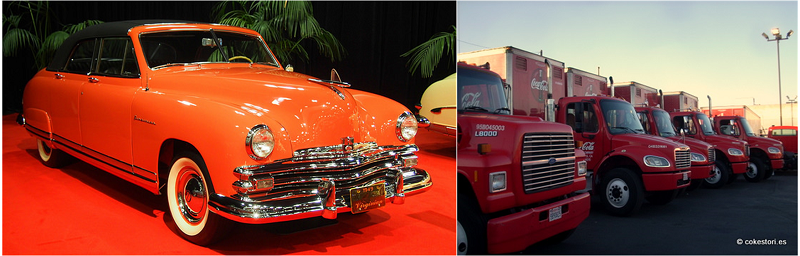
\includegraphics[width=0.48\textwidth]{images/1_02-vehicles.png}}}}{collectible car}
\end{center}
\caption[{Collectible car versus fleet vehicles }]{Collectible car versus fleet vehicles \footnotemark{}}
\end{wrapfigure}
\end{sidebar}
 
For further information and practical examples, see \emph{Infrastructure as Code} by Kief Morris \hyperlink{Morris2016}{[Morris2016]}.
 
\label{version-control}\hyperlabel{version-control}
   
\subsection{Configuration management: the basics}
\label{_configuration_management_the_basics}\hyperlabel{_configuration_management_the_basics}%
  
Configuration management is a critically important practice in digital systems, and has always been so. How it is performed has evolved over time. At this stage in our journey, we are one or two people in a startup, working with digital artifacts such as our \hyperlink{infra-code-example}{iac.sh example} discussed in the previous section.
 
One or two people can achieve an impressive amount with modern digital platforms. But the work is complex. Tracking and controlling your work products as they evolve through change after change is important from day one of your efforts. It's not something you want to put off to "later when I have time." This applies to computer code, configurations, and increasingly even documentation (often written in a lightweight markup language like Markdown or Asciidoc). In terms of infrastructure, configuration management requires three capabilities:
 \begin{itemize}

\item{} The ability to back up or archive a system's operational state (in general, not including the data it is processing -{} that is a different concern). Taking the backup should not require taking the system down.
 

\item{} The ability to compare two versions of the system's state and identify differences
 

\item{} The ability to restore the system to a previously archived operational state.
 
\end{itemize}
 
In this section, we will discuss the following topics:
 \begin{itemize}

\item{} Version control
 

\item{} Source control
 

\item{} Package management
 

\item{} Deployment management
 

\item{} Configuration management
 
\end{itemize}
 
and their relationships.
 
\subsubsection{What is version control?}
\label{_what_is_version_control}\hyperlabel{_what_is_version_control}%
  \begin{quote}

In software development, version control is the foundation of every other Agile technical practice. Without version control, there is no build, no TDD, no continuous integration.

\hspace*\fill--- Andrew Clay Shafer
\emph{Web Operations:Keeping the Data On Time} \end{quote}
 
The Agile Alliance indicates \textquotedblleft{}version control\textquotedblright{} as one of the \href{https://www.agilealliance.org/agile101/subway-map-to-agile-practices/}{four foundational areas of Agile} \hyperlink{Alliance2016}{[Alliance2016]}, along with team, iterative development, and incremental development. Why is this? Version control is critical for any kind of system with complex, changing content, especially when many people are working on that content. Version control provides the capability of seeing the exact sequence of a complex system's evolution and isolating any particular moment in its history, or providing detailed analysis on how two versions differ. With version control, we can understand what changed and when, which is essential to coping with complexity.
 
While version control was always deemed important for software artifacts, it has only recently become the preferred paradigm for managing infrastructure state as well.  Because of this, version control is possibly the first IT management system you should acquire and implement (perhaps as a cloud service, such as Github).
 
Version control in recent years increasingly distinguishes between source and package management: the management of binary files, as distinct from human-{}understandable symbolic files. There is also a need to understand what versions are installed on what computers; this can be termed "deployment management." (With the advent of containers, this is a particularly fast changing area.)
 \begin{wrapfigure}{r}{0.5\textwidth}[H]

\begin{center}
\imgexists{images/1_02-versionControlTypes.png}{{\imgevalsize{images/1_02-versionControlTypes.png}{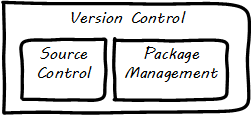
\includegraphics[width=0.48\textwidth]{images/1_02-versionControlTypes.png}}}}{Version control types}
\end{center}
\caption{Types of version control}
\end{wrapfigure}
 
Version control works like an advanced file system with a memory. (Actual file systems that do this are called \href{https://en.wikipedia.org/wiki/Versioning_file_system}{\emph{versioning}} file systems.) It can remember all the changes you make to its contents, tell you the differences between any two versions, and also bring back the version you had at any point in time. Version control is important -{} but how important? Survey research presented in the annual State of DevOps report indicates that version control is one of the most critical practices associated with high performing IT organizations \hyperlink{Forsgren2016}{[Forsgren2016]}. Nicole Forsgren \hyperlink{Forsgren2016a}{[Forsgren2016a]}  summarizes the practice of version control as:
 \begin{itemize}

\item{} Our application code is in a version control system
 

\item{} Our system configurations are in a version control system
 

\item{} Our application configurations are in a version control system
 

\item{} Our scripts for automating build and configuration are in a version control system.
 
\end{itemize}
 
\paragraph{Source control}
\label{_source_control}\hyperlabel{_source_control}%
  
Digital systems start with text files, typically encoded in \href{https://en.wikipedia.org/wiki/ASCII}{ASCII}. Text editors create source code, scripts, and configuration files. These may be transformed in defined ways (e.g. by compilers and build tools) but the human understandable end of the process is mostly based on text files. In the previous section, we described a \hyperlink{infra-code-example}{simple script} that altered the state of a computer system. We care very much about when such a text file changes. One wrong character can completely alter the behavior of a large, complex system. Therefore, our configuration management approach must track to that level of detail.
 
Source control is at its most powerful when dealing with textual data. It is less useful in dealing with  binary data, such as image files. Text files can analyzed for their differences in an easy to understand way. If I change "abc" to "abcd" it is clear that the third character has been changed from \textquotedblleft{}c\textquotedblright{} to \textquotedblleft{}d.\textquotedblright{} On the other hand, if I take a picture (e.g. as a *.png file) and alter one pixel, and compare the resulting before and after binary files in terms of their data, it would be more difficult to understand what had changed. I might be able to easily tell that they are two different files, but they would look very similar and the difference in the binary data might be difficult to understand. Here is a detailed demonstration, using the command line in Ubuntu Linux. (Don't worry, we will explain what is going on.)
 \begin{DBKadmonition}{}{Note}
 
In the below sequence, what you see after the "\$" sign is what is being typed. If there is no "\$" sign, it is what the system is saying in response.
 \end{DBKadmonition}
 
First, we create a directory (similar to the \hyperlink{infra-code-example}{iac.sh example script}):
 
\begin{lstlisting}[firstnumber=1,backgroundcolor={},basicstyle=\ttfamily,]
~$ mkdir tmpgit
\end{lstlisting}
 
Then, we navigate to it:
 
\begin{lstlisting}[firstnumber=1,backgroundcolor={},basicstyle=\ttfamily,]
~$ cd tmpgit/
\end{lstlisting}
 
And activate git source control:
 
\begin{lstlisting}[firstnumber=1,backgroundcolor={},basicstyle=\ttfamily,]
~/tmpgit$ git init
Initialized empty Git repository in /home/char/tmpgit/.git/
\end{lstlisting}
 
We create a simple program:
 
\begin{lstlisting}[firstnumber=1,backgroundcolor={},basicstyle=\ttfamily,]
~/tmpgit$ echo 'print "hello world!";' > tmp.py
\end{lstlisting}
 
And run it:
 
\begin{lstlisting}[firstnumber=1,backgroundcolor={},basicstyle=\ttfamily,]
~/tmpgit$ python tmp.py
hello world!
\end{lstlisting}
 
We stage it for source control:
 
\begin{lstlisting}[firstnumber=1,backgroundcolor={},basicstyle=\ttfamily,]
~/tmpgit$ git add . tmp.py
\end{lstlisting}
 
And commit it:
 
\begin{lstlisting}[firstnumber=1,backgroundcolor={},basicstyle=\ttfamily,]
~/tmpgit$ git commit -m "first commit"
[master (root-commit) cabdbe3] first commit
1 file changed, 1 insertion(+)
create mode 100644 tmp.py
\end{lstlisting}
 
The file is now under version control. We can change our working copy and run it:
 
\begin{lstlisting}[firstnumber=1,backgroundcolor={},basicstyle=\ttfamily,]
~/tmpgit$ echo 'print "hello universe\n";' > tmp.py
~/tmpgit$ python tmp.py
hello universe!
\end{lstlisting}
 
When the "echo" command is run with just one ">{}" it replaces the data in the target file completely. So we have completely replaced "hello world!" with "hello universe!"
 
And -{} \textbf{most critically} -{} we can see what we have changed!
 
\begin{lstlisting}[firstnumber=1,backgroundcolor={},basicstyle=\ttfamily,]
~/tmpgit$ git diff
diff --git a/tmp.py b/tmp.py
index 0ecbd83..a203522 100644
--- a/tmp.py
+++ b/tmp.py
@@ -1 +1 @@
-print "hello world!";
+print "hello universe!";
\end{lstlisting}
 
Notice the "-{}" (minus) sign before 'print "hello world!";'\hspace{0.167em}\textemdash{}\hspace{0.167em}that means it has been deleted. The "+" (plus) sign before 'print "hello universe!";' means that line has been added.
 
We can restore the original file (note that this eradicates the working change we made!)
 
\begin{lstlisting}[firstnumber=1,backgroundcolor={},basicstyle=\ttfamily,]
char@elsa:~/tmpgit$ git checkout .
char@elsa:~/tmpgit$ python tmp.py
hello world!
\end{lstlisting}
 
If you have access to a Linux computer, try it! (It should also work on recent Macs as presented here.)
 
In comparison, the following are two 10x10 gray-{}scale bitmap images being edited in the \href{https://www.gimp.org/}{Gimp image editor}. They are about as simple as you can get. Notice that they are slightly different:
 \begin{wrapfigure}{r}{0.5\textwidth}[H]

\begin{center}
\imgexists{images/1_02-bothPixels.png}{{\imgevalsize{images/1_02-bothPixels.png}{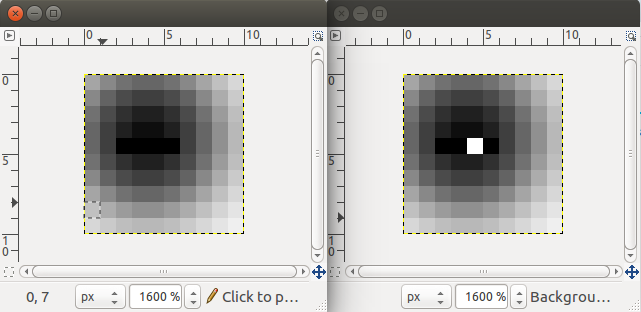
\includegraphics[width=0.48\textwidth]{images/1_02-bothPixels.png}}}}{grid}
\end{center}
\caption{Bitmap images}
\end{wrapfigure}
 
If we save these in the *.png format, we can see they are different sizes (242 k vs 239k). But if we open them in a binary editor it is very difficult to understand how they differ:
 \begin{wrapfigure}{r}{0.5\textwidth}[H]

\begin{center}
\imgexists{images/1_02-pixelHex1.png}{{\imgevalsize{images/1_02-pixelHex1.png}{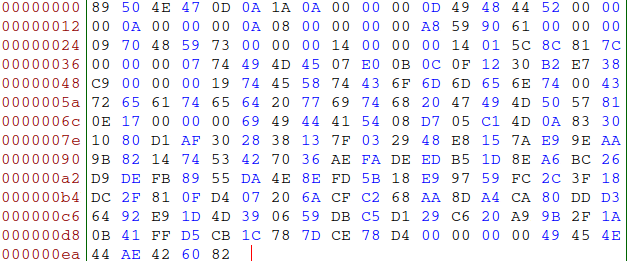
\includegraphics[width=0.48\textwidth]{images/1_02-pixelHex1.png}}}}{data}
\end{center}
\caption{First image binary data}
\end{wrapfigure}
 \begin{wrapfigure}{r}{0.5\textwidth}[H]

\begin{center}
\imgexists{images/1_02-pixelHex2.png}{{\imgevalsize{images/1_02-pixelHex2.png}{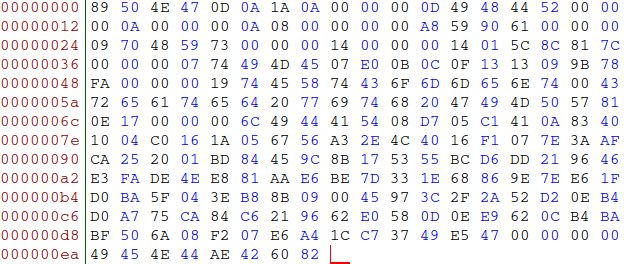
\includegraphics[width=0.48\textwidth]{images/1_02-pixelHex2.png}}}}{data}
\end{center}
\caption{Second image binary data}
\end{wrapfigure}
 
Even if we analyzed the differences, we would need to know much about the .png format in order to understand how the two images differ. We can still track both versions these files, of course, with the proper version control. But again, binary data is not ideal for source control tools like git.
  
\paragraph{The "commit" concept}
\label{_the_commit_concept}\hyperlabel{_the_commit_concept}%
  
Although implementation details may differ, all version control systems have some concept of \textquotedblleft{}commit.\textquotedblright{} As stated in \emph{Version Control with Git} \hyperlink{Loeliger2009}{[Loeliger2009]}:
 
\emph{In Git, a commit is used to record changes to a repository\ldots{} Every Git commit represents a single, \textbf{atomic} changeset with respect to the previous state. Regardless of the number of directories, files, lines, or bytes that change with a commit\ldots{} either all changes apply or none do.} [emphasis added]
 \begin{DBKadmonition}{}{Note}
 
*Why "atomic"? The word atomic derives from the ancient Latin language, and means "indivisible." An atomic set of changes is either entirely applied, or entirely rejected. Atomicity is an important concept in computing, and transaction processing in particular. If our user tries to move money from her savings to her checking account, two operations are required: (1) reduce savings and (2) increase checking. Either both need to succeed, or both need to fail. That is the classic definition of an "atomic" transaction. Version control commits should be atomic.
 \end{DBKadmonition}
 
The concept of a version or source control \href{https://en.wikipedia.org/wiki/Commit_(data_management)}{\textquotedblleft{}commit\textquotedblright{}} is a rich foundation for IT management and governance. It both represents the state of the computing system as well as providing evidence of the human activity affecting it. As we will see in Chapter 3, the \textquotedblleft{}commit\textquotedblright{} identifier is directly referenced by build activity, which in turn is referenced by the release activity, which is typically visible across the IT value chain.
 
Also, the concept of an atomic \textquotedblleft{}commit\textquotedblright{} is essential to the concept of a \textquotedblleft{}branch\textquotedblright{} -{} the creation of an experimental version, completely separate from the main version, so that various alterations can be tried without compromising the overall system stability. Starting at the point of a \textquotedblleft{}commit,\textquotedblright{} the branched version also becomes evidence of human activity around a potential future for the system. In some environments, the branch is automatically created with the assignment of a requirement or story -{} again, more on this to come in chapter 3. In other environments, the very concept of branching is avoided.
 
\label{package-mgmt}\hyperlabel{package-mgmt}
   
\subsubsection{Package management}
\label{_package_management}\hyperlabel{_package_management}%
  \begin{quote}

Implement version control for all production artifacts.

\hspace*\fill--- Puppet Labs 2015 State of DevOps report
\end{quote}
 
In some organizations, it was once common for compiled binaries to be stored in the same repositories as source code. However, this is no longer considered a best practice. Source and package management are now viewed as two separate things.  Source repositories should be reserved for text-{}based artifacts whose differences can be made visible in a human-{}understandable way. Package repositories in contrast are for binary artifacts that can be deployed.
 
Package repositories also can serve as a proxy to the external world of downloadable software. That is, they are a cache, an intermediate store of the software provided by various "upstream" sources. For example, developers may be told to download the approved Ruby on Rails version from the local package repository, rather than going to the getting the latest version, which may not be suitable for the environment.
 
Package repositories are also used to enable collaboration between teams working on large systems. Teams can check in their built components into the package repository for other teams to download. This is more efficient than everyone  always building all parts of the application from the source repository.
 
The boundary between source and package is not hard and fast, however. One does see binary files in source repositories, such as images used in an application. Also, when interpreted languages (such as Javascript) are "packaged," they still appear in the package as text files, perhaps compressed or otherwise incorporated into some larger containing structure.
 
\label{deployment-mgmt}\hyperlabel{deployment-mgmt}
  
\subsubsection{Deployment management}
\label{_deployment_management}\hyperlabel{_deployment_management}%
  
Version control is an important part of the overall concept of configuration management. But configuration management also covers the matter of how artifacts under version control are combined with other IT resources (such as virtual machines) to deliver services. The following illustration is one way to think about the relationships:
 \begin{wrapfigure}{r}{0.5\textwidth}[H]

\begin{center}
\imgexists{images/1_02-configMgmt.png}{{\imgevalsize{images/1_02-configMgmt.png}{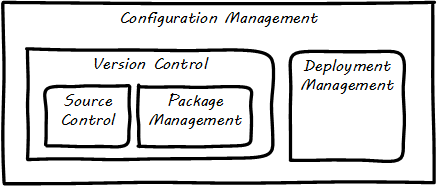
\includegraphics[width=0.48\textwidth]{images/1_02-configMgmt.png}}}}{Configuration management types}
\end{center}
\caption{Configuration management and its components}
\end{wrapfigure}
 
\paragraph{Deployment basics}
\label{_deployment_basics}\hyperlabel{_deployment_basics}%
  
Resources in version control in general are not yet active in any value-{}adding sense. In order for them to deliver experiences, they must be combined with computing resources: servers (physical or virtual), storage, nettworking, and the rest, whether owned by the organization or leased as \hyperlink{cloud}{Cloud services}. The process of doing so is called deployment. Version control manages the state of the artifacts; deployment management (as another configuration management practice) manages the \textbf{combination of those artifacts with the needed resources for value delivery}.
 
\label{policy-config}\hyperlabel{policy-config}
  
\paragraph{Imperative and Declarative}
\label{_imperative_and_declarative}\hyperlabel{_imperative_and_declarative}%
  
Before we turned to source control, we looked at a \hyperlink{infra-code-example}{simple script} that changed the configuration of a computer. It did so in an \emph{imperative} fashion. Imperative and declarative are two important terms from computer science.
 

\begin{sidebar}
\textbf{A simple example of \textquotedblleft{}declarative\textquotedblright{} vs \textquotedblleft{}imperative\textquotedblright{}}


\textbf{Declarative:} "Our refrigerator should always have a gallon of milk in it.\textquotedblright{}

\textbf{Imperative:} \textquotedblleft{}Go out the door, take a right, take a left, go into the building with a big `SA' on it, go in to the last aisle, take a left, go to the third case and take the first container on the fourth shelf from the bottom. Give money to the cashier and bring the container back home.\textquotedblright{}
\end{sidebar}
 
In an imperative approach, we tell the computer specifically how we want to accomplish a task, e.g.:
 \begin{enumerate}[label=\arabic*.]

\item{} Create a directory
 

\item{} Create some files
 

\item{} Create another directory
 

\item{} Create more files
 
\end{enumerate}
 
And so on. Many traditional programming languages take an imperative approach. A script such as \hyperlink{infra-code-example}{iac.sh example} is executed line by line, i.e., it is imperative. In configuring infrastructure, scripting is in general considered \textquotedblleft{}imperative," but state of the art infrastructure automation frameworks are built using a \textquotedblleft{}declarative,\textquotedblright{} policy-{}based approach, in which the object is to define the desired end state of the resource, not the steps needed to get there.  With such an approach, instead of defining a set of steps, we simply define the proper configuration as a target, saying (in essence) that "this computer should always have a directory structure thus; do what you need to do to make it so and keep it this way."
 
More practically, declarative approaches are used to ensure that the proper versions of software are always present on a system, and that configurations such as Internet ports and security settings do not vary from the intended specification.
 
This is a complex topic and there are advantages and disadvantages to each approach. (See "When and Where Order Matters" by Mark Burgess for an advanced discussion \hyperlink{Burgess2016}{[Burgess2016]}.) But policy-{}based approaches seem to have the upper hand for now.
    
\subsection{Topics in IT infrastructure}
\label{_topics_in_it_infrastructure}\hyperlabel{_topics_in_it_infrastructure}%
  
This and following chapters in this book will end with a "topics" section, in which current and specialized developments will be discussed.
 
\label{commit-as-metadata}\hyperlabel{commit-as-metadata}
 
\subsubsection{Configuration management, version control, and metadata}
\label{_configuration_management_version_control_and_metadata}\hyperlabel{_configuration_management_version_control_and_metadata}%
  
Version control, in particular source control, is where we start to see the emergence of an \emph{architecture of IT management}. It is in the source control system that we first start to see \emph{metadata} emerge as an independent concern. Metadata is a tricky term, that tends to generate confusion. The term \textquotedblleft{}meta\textquotedblright{} implies a concept that is somehow self-{}referential, and/or operating at a higher level of abstraction. So,
 \begin{itemize}

\item{} the term meta-{}discussion is a discussion about the discussion;
 

\item{} meta-{}cognition is cognition about cognition, and
 

\item{} meta-{}data (aka metadata) is data about data.
 
\end{itemize}
 
Some examples:
 \begin{itemize}

\item{} In traditional data management, metadata is the description of the data structures, especially from a business point of view. A database column might be named \textquotedblleft{}CUST\_L\_NM,\textquotedblright{} but the business description or metadata would be \textquotedblleft{}The last, family, or surname of the customer.\textquotedblright{}
 

\item{} In document management, the document metadata is the record of who created the document and when, when it was last updated, and so forth. Failure to properly sanitize document metadata has led to various privacy and data security related issues.
 

\item{} In telephony,  \textquotedblleft{}data\textquotedblright{} is the actual call signal \textemdash{} the audio of the phone conversation, nowadays usually digitally encoded. Metadata on the other hand is all the information about the call: from who to who, when, how long, and so forth.
 
\end{itemize}
 
In computer systems, metadata can be difficult to isolate. Sometimes, computing professionals will speak of a \textquotedblleft{}metadata\textquotedblright{} layer that may define physical database structures, data extracts, business process behavior, even file locations. The trouble is, from a computer's point of view, a processing instruction is an instruction, and the prefix \textquotedblleft{}meta\textquotedblright{} has no real meaning.
 
Because of this, this book favors a principle that \textbf{metadata is by definition non-{}runtime.} It is documentation, usually represented as structured or semi-{}structured data, but not usually a primary processing input or output. It might be \textquotedblleft{}digital exhaust\textquotedblright{} -{} log files are a form of metadata. It is not executable. If it's  executable (directly or indirectly), it's digital logic or configuration, plain and simple.
 
So what about our infrastructure as code example? The artifact -{} the configuration file, the script -{} is NOT metadata, because it is executable. But the source repository commit IS metadata. It has no meaning for the script. The dependency is one way -{} without the artifact, the commit ID is meaningless, but the artifact is completely ignorant of the commit. The commit may become an essential data point for human beings trying to make sense of the state of a resource defined by that artifact. However, the version control system \ldots{}\hspace{0em}
 
\emph{doesn't care why files are changing. That is, the content of the changes doesn't matter. As the developer, you might move a function from here to there and expect this to be handled as one unitary move. But you could, alternatively, commit the removal and then later commit the addition. Git doesn't care. It has nothing to do with the semantics of what is in the files} \hyperlink{Loeliger2009}{[Loeliger2009]}.
 
\textbf{In this microcosm, we see the origins of IT management.} It is not always easy to apply this approach in practice. There can be edge cases. Documentation stored in version control needs to be seen as "executable" in the context of the business process. But it too does not require or "know about" the comit. Ultimately \textbf{the concept of metadata provides a basis for distinguishing the \emph{management} of information technology from the actual \emph{practice} of information technology.}
 
\begin{lstlisting}[firstnumber=1,backgroundcolor={},basicstyle=\ttfamily,]
===== Operations basics
Just enough Operations for the startup
Prep chap 6
\end{lstlisting}
 
\begin{lstlisting}[firstnumber=1,backgroundcolor={},basicstyle=\ttfamily,]
Open Compute standard
\end{lstlisting}
 
\begin{lstlisting}[firstnumber=1,backgroundcolor={},basicstyle=\ttfamily,]
===== additional material
\end{lstlisting}
 
\begin{lstlisting}[firstnumber=1,backgroundcolor={},basicstyle=\ttfamily,]
http://12factor.net/build-release-run
\end{lstlisting}
 
\begin{lstlisting}[firstnumber=1,backgroundcolor={},basicstyle=\ttfamily,]
Releases are an append-only ledger and a release cannot be mutated once it is created. Any change must create a new release.
\end{lstlisting}
 
\begin{lstlisting}[firstnumber=1,backgroundcolor={},basicstyle=\ttfamily,]
In the old world, environments were accepted to be different except where they needed to be consistent. In the new world, environments are assumed to be the same except where they need to be different.
\end{lstlisting}
 
\begin{lstlisting}[firstnumber=1,backgroundcolor={},basicstyle=\ttfamily,]
what makes a good infrastructure engineer
\end{lstlisting}
 
\begin{lstlisting}[firstnumber=1,backgroundcolor={},basicstyle=\ttfamily,]
==== more on policy & config
\end{lstlisting}
 
\begin{lstlisting}[firstnumber=1,backgroundcolor={},basicstyle=\ttfamily,]
define idempotence
\end{lstlisting}
 
\begin{lstlisting}[firstnumber=1,backgroundcolor={},basicstyle=\ttfamily,escapeinside={<:}{:>}]
Two important concepts have emerged in the past decade: policy-based management and promise theory. In brief, policy-based management and promise theory focus on <:\textquotedblleft{}:>what,<:\textquotedblright{}:> not <:\textquotedblleft{}:>how.<:\textquotedblright{}:> This may also be described as <:\textquotedblleft{}:>declarative,<:\textquotedblright{}:> not <:\textquotedblleft{}:>imperative<:\textquotedblright{}:> (see Sidebar).
\end{lstlisting}
 
\begin{lstlisting}[firstnumber=1,backgroundcolor={},basicstyle=\ttfamily,]
For example, the following shell script and Chef recipe do the same thing:
\end{lstlisting}
 
\begin{lstlisting}[firstnumber=1,backgroundcolor={},basicstyle=\ttfamily,escapeinside={<:}{:>}]
create example - can<:':>t find anything decent on web
Use directory creation example with failure of script b/c not idempotent
\end{lstlisting}
 
\begin{lstlisting}[firstnumber=1,backgroundcolor={},basicstyle=\ttfamily,]
Increasingly, as operational performance is defined in code (the trend to Infrastructure as Code), operational issues are equivalent to development defects.
\end{lstlisting}
 
\begin{lstlisting}[firstnumber=1,backgroundcolor={},basicstyle=\ttfamily,]
===== Cloud transition
\end{lstlisting}
 
\begin{lstlisting}[firstnumber=1,backgroundcolor={},basicstyle=\ttfamily,]
http://jpmorgenthal.com/2016/08/24/a-reality-check-on-everyones-moving-everything-to-the-cloud/ excellent
\end{lstlisting}
 
\begin{lstlisting}[firstnumber=1,backgroundcolor={},basicstyle=\ttfamily,]
choreography & orchestration - John Willis convo
\end{lstlisting}
 
\begin{lstlisting}[firstnumber=1,backgroundcolor={},basicstyle=\ttfamily,]
risk management & infrastructure choices (Charity Majors talk 7/21/2016 DevOpsDays MSP)
\end{lstlisting}
 
\begin{lstlisting}[firstnumber=1,backgroundcolor={},basicstyle=\ttfamily,]
===== Architecture of IT management
\end{lstlisting}
 
\begin{lstlisting}[firstnumber=1,backgroundcolor={},basicstyle=\ttfamily,escapeinside={<:}{:>}]
The concept of a version control system (variously known as source control, revision control, software configuration management, and other terms) is our first major software system for the <:\textquotedblleft{}:>business of IT.<:\textquotedblright{}:> (The virtualized system previously discussed is what is *under management*; the source control system is part of the *management architecture*.)
\end{lstlisting}
 
\begin{lstlisting}[firstnumber=1,backgroundcolor={},basicstyle=\ttfamily,]
_describe modern infra managers, policy management, auto-scaling as an example, provide an example Chef script.._
\end{lstlisting}
   
\subsection{Conclusion}
\label{_conclusion}\hyperlabel{_conclusion}%
  
Books and articles are written every week about some aspect of IT infrastructure. We have only scratched the surface in our discussions of compute, network, and storage, and how they have become utility services in the guise of Cloud. Software as a service, platform as a service, infrastructure as a service -{} each represents a different approach. For the most part, we will focus on Infrastructure as a Service in the remainder of this book, on the assumption that your digital product is unique enough to need the broad freedom this provides.
 
IT infrastructure is a rich and complex topic, and a person can spend their career specializing in it. For this class, we always want to keep chapter 1 in mind: why do we want it? How does it provide for our needs, contribute to our enjoyment? There are numerous sources available to you to learn Linux scripting, policy-{}based configuration management of infrastructure, and source control. Competency with source control is essential to your career and you should devote some serious time to it. You can find many references to source control on the Internet and in books such as \emph{Pro Git} by Scott Chacon and Ben Straub \hyperlink{Chacon2009}{[Chacon2009]}. As it is the most important foundational technology for professional IT, whether in a garage or in the largest organizations, you need to have a deep familiarity with it.
 
We will discuss further infrastructure issues in Chapter 6, including designing systems for failure and availability.
 
\subsubsection{Discussion questions}
\label{_discussion_questions_2}\hyperlabel{_discussion_questions_2}%
  \begin{enumerate}[label=\arabic*.]

\item{} Consider your product idea from the previous chapter. Does it have any particular infrastructure needs you can identify, having read this chapter?
 

\item{} Your personal laptop or smart phone is infrastructure. What issues have you had with it? Have you had to change its configuration?
 

\item{} Would you prefer to build your product on an IaaS or PaaS platform (see \hyperlink{cloud-models}{the Cloud models})? Is there an SaaS product that might serve? (If so, what is your value-{}adding idea?)
 

\item{} Compare the costs of Cloud to owning your own server. Assume you buy a server inexpensively on EBay and put it in your garage. What other factors might you consider before doing this?
 
\end{enumerate}
  
\subsubsection{Research \& practice}
\label{_research_practice_2}\hyperlabel{_research_practice_2}%
  \begin{enumerate}[label=\arabic*.]

\item{} Research Cloud providers and recommend which you would prefer to build your new product on.
 

\item{} Interview someone who has worked in a data center as to what a "day in the life" is, and how it's changed for them.
 

\item{} Install Vagrant and Virtualbox on your personal device and bring up a Linux virtual machine. Run a Linux tutorial.
 

\item{} Configure a declarative infrastructure manager (Chef, Puppet, Ansible, or Salt Stack) to control your Vagrant VMs. Use git to control your configurations.
 

\item{} Install Docker and run a tutorial on it.
 
\end{enumerate}
  
\subsubsection{Further reading}
\label{_further_reading_2}\hyperlabel{_further_reading_2}%
  
\textbf{Books}
 \begin{itemize}

\item{} Thomas A. Limoncelli, Strata R. Chalup, Christina J. Hogan, \href{http://www.goodreads.com/book/show/23131211-the-practice-of-cloud-system-administration}{The Practice of Cloud System Administration: Designing and Operating Large Distributed Systems, Volume 2}
 

\item{} John Allspaw, \href{http://www.goodreads.com/book/show/8571725-web-operations}{Web Operations: Keeping the Data On Time}
 

\item{} Kief Morris, \href{https://www.goodreads.com/book/show/26544394-infrastructure-as-code}{Infrastructure as Code: Managing Servers in the Cloud}
 

\item{} Ellen Siever, Stephen Figgins, Robert Love (Goodreads Author), Arnold Robbins, Aaron Weber, \href{http://www.goodreads.com/book/show/227148.Linux_in_a_Nutshell}{Linux in a Nutshell}
 

\item{} Scott Chacon, \href{http://www.goodreads.com/book/show/6518085-pro-git?}{Pro Git}
 

\item{} Mark Burgess, \href{https://www.goodreads.com/book/show/261632.Analytical_Network_and_System_Administration}{Analytical Network and System Administration: Managing Human-{}Computer Systems} (\emph{exceptionally deep and rigorous book by a trained physicist on using mathematical methods to understand computing infrastructure problems.})
 
\end{itemize}
 
\textbf{Articles}
 \begin{itemize}

\item{} \href{http://www.lauradhamilton.com/servers-pets-versus-cattle}{Are your servers pets or cattle?}
 

\item{} \href{http://vmboomerang.com/posts/cloud-jumping-why-amazon-aws-is-kicking-paas/}{Clouds Jumping \textendash{} Why AWS Is Kicking PaaS}
 

\item{} \href{http://jpmorgenthal.com/2016/08/24/a-reality-check-on-everyones-moving-everything-to-the-cloud/}{A reality check on everyone moving everything to the Cloud}
 

\item{} \href{https://gist.github.com/jboner/2841832}{Latency Numbers Every Programmer Should Know}
 

\item{} \href{http://csrc.nist.gov/publications/nistpubs/800-145/SP800-145.pdf}{NIST definition of Cloud computing}
 

\item{} \href{http://www.wired.com/2015/09/google-2-billion-lines-codeand-one-place/}{Google Is 2 Billion Lines of Code\textemdash{}And It's All in One Place}
 

\item{} \href{http://continuousdelivery.com/2011/07/on-dvcs-continuous-integration-and-feature-branches/}{On DVCS, continuous integration, and feature branches}
 

\item{} \href{http://markburgess.org/blog_order.html}{When and Where Order Matters}
 
\end{itemize}
 
\label{chapter-app-deliv}\hyperlabel{chapter-app-deliv} \label{chapter-3}\hyperlabel{chapter-3}
    
\section{Chapter 3: Application Delivery}
\label{_chapter_3_application_delivery}\hyperlabel{_chapter_3_application_delivery}%
  

\begin{sidebar}

\textbf{Collaborative}

\begin{lstlisting}[firstnumber=1,backgroundcolor={},basicstyle=\ttfamily,]
Status 11/2016: This chapter is in "draft 1.5" - improved from original first draft completed in 2015.
\end{lstlisting}
\begin{itemize}

\item{} \href{https://github.com/dm-academy/aitm/blob/master/collaborator-instructions.adoc}{Collaborator instructions}
 

\item{} Raise an \href{https://github.com/dm-academy/aitm/issues}{issue} to comment
 

\item{} \href{https://github.com/dm-academy/aitm/tree/master/book}{Github source files}
 
\end{itemize}

\emph{Please remember that the intended audience of this one or two semester survey text is incoming students at a Masters' level in Information Technology, Information Systems, and Software Engineering programs. The most useful feedback comes from the perspective of, "what do you think today's students need to learn, given the last 20 years' developments with Agile, Lean IT, DevOps, web-{} and cloud-{}scale IT, digital transformation, and related themes?"}
\end{sidebar}
 

\begin{sidebar}
\textbf{Instructor's note}


I have opted to defer the "theory" of Agile to Parts II and III. So, this chapter presents Agile and related concepts like iterative development without examining the underlying principles.

I do this because I have discovered that theory sometimes works better in retrospect. Many students increasingly come in with some exposure to Cloud and Agile methods at least, and Chapters 2 and 3 will seem comfortable and familiar. In Chapters 4 and on we challenge them with \textbf{why} Agile works.
\end{sidebar}
 
\subsection{Introduction}
\label{_introduction_3}\hyperlabel{_introduction_3}%
  
Now that we have some idea of IT value (and how we might turn it into a product), and have decided on some infrastructure, we can start building.
 
IT systems that directly create value for non-{}technical users are usually called "applications," or sometimes "services." As discussed in chapter 1, they enable value experiences in areas as diverse as consumer banking, entertainment and hospitality, and personal transportation. In fact it is difficult to think of any aspect of modern life untouched by applications. (This overall trend is sometimes called digital transformation.)
 
Applications are built from software, the development of which is a core concern for any IT-{}centric product strategy. Software development is a well established career, and a fast-{}moving field with new technologies, frameworks, and schools of thought emerging weekly, it seems. This chapter will cover applications and the software lifecycle, from requirements through construction, testing, building, and deployment into modern production environments. It also discusses earlier approaches to software development, the rise of the Agile movement, and its current manifestation in the practice of DevOps.
 
\subsubsection{Chapter outline}
\label{_chapter_outline_2}\hyperlabel{_chapter_outline_2}%
  \begin{itemize}

\item{} Introduction
 

\item{} Learning objectives
 

\item{} Basics of applications and their development
 \begin{itemize}

\item{} Defining "Application"
 

\item{} History of applications and application software
 

\item{} Applications and infrastructure: the old way
 

\item{} Applications and infrastructure today
 
\end{itemize}
 

\item{} From waterfall to Agile
 

\item{} The DevOps challenge
 

\item{} Describing system intent
 

\item{} Test-{}driven development and refactoring
 \begin{itemize}

\item{} Test-{}driven development
 

\item{} Refactoring
 
\end{itemize}
 

\item{} Continuous integration
 

\item{} Continuous deployment
 

\item{} Application development topics
 

\item{} Conclusion
 \begin{itemize}

\item{} Discussion questions
 

\item{} Research \& practice
 

\item{} Further reading
 
\end{itemize}
 
\end{itemize}
  
\subsubsection{Learning objectives}
\label{_learning_objectives_2}\hyperlabel{_learning_objectives_2}%
  \begin{itemize}

\item{} Understand history and importance of "application" concept
 

\item{} Define "Agile" in terms of software development
 

\item{} Identify key Agile practices
 

\item{} Identify the major components of an end-{}to-{}end DevOps delivery pipeline.
 
\end{itemize}
   
\subsection{Basics of applications and their development}
\label{_basics_of_applications_and_their_development}\hyperlabel{_basics_of_applications_and_their_development}%
  
\subsubsection{Defining "Application"}
\label{_defining_application}\hyperlabel{_defining_application}%
  
In keeping with our commitment to theory and first principles, we use an engineering definition of "application." To an electrical engineer, a toaster or a light bulb is an "application" of electricity. Similarly, a customer relationship management system, or a Web video on demand service, are "applications" of the core computer infrastructure we studied in the last chapter.
  
\subsubsection{History of applications and application software}
\label{_history_of_applications_and_application_software}\hyperlabel{_history_of_applications_and_application_software}%
  \begin{wrapfigure}{r}{0.5\textwidth}[H]

\begin{center}
\imgexists{images/1_03-Eniac.jpg}{{\imgevalsize{images/1_03-Eniac.jpg}{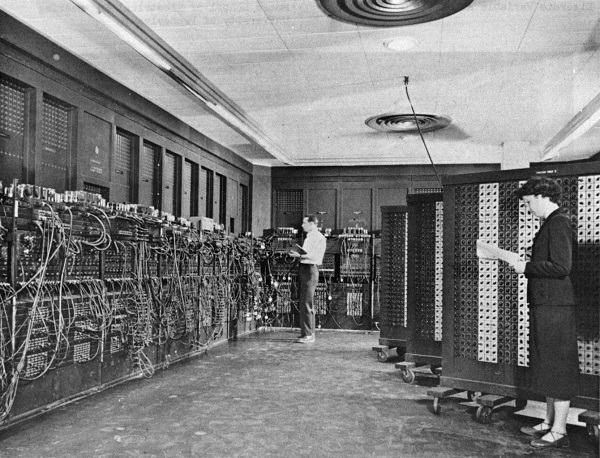
\includegraphics[width=0.48\textwidth]{images/1_03-Eniac.jpg}}}}{old computer room}
\end{center}
\caption[{The ENIAC\hspace{0.167em}\textemdash{}\hspace{0.167em}"programmed" by cable reconfiguration. }]{The ENIAC\hspace{0.167em}\textemdash{}\hspace{0.167em}"programmed" by cable reconfiguration. \footnotemark{}}
\end{wrapfigure}
 
Without applications, computers would be merely a curiousity. Computers were first "applied" to military needs for codebreaking and artillery calculations. After World War II, ex-{}military officers like \href{https://en.wikipedia.org/wiki/Edmund_Berkeley}{Edmund Berkeley} at Prudential realized their potential if "applied" to problems like insurance record keeping. \hyperlink{Akera2007}{[Akera2007]} At first, such systems required actual manual configuration (as in the ENIAC photo in this section), or painstaking programming in complex, tedious, and unforgiving \href{https://en.wikipedia.org/wiki/Low-level_programming_language}{low-{}level programming languages}. As the value of computers became obvious, investment was made in making programming easier through more powerful languages.
 
The  \href{https://en.wikipedia.org/wiki/History_of_software}{history of software} is well documented. Low level languages (\href{https://en.wikipedia.org/wiki/Binary_code}{binary} and \href{https://en.wikipedia.org/wiki/Assembly_language}{assembler}) were increasingly replaced by higher level languages (\href{https://en.wikipedia.org/wiki/Fortran}{FORTRAN}, \href{https://en.wikipedia.org/wiki/COBOL}{COBOL}, \href{https://en.wikipedia.org/wiki/C_(programming_language)}{C}). Proprietary machine/language combinations were replaced by open standards and \href{https://en.wikipedia.org/wiki/Compiler}{compilers} that could take one kind of source code and build it for different hardware platforms. Many languages followed, such as \href{https://en.wikipedia.org/wiki/Java_(programming_language)}{Java}, \href{https://en.wikipedia.org/wiki/Visual_Basic}{Visual Basic}, and \href{https://www.javascript.com/}{Javascript}. Extensive middleware was developed to enable ease of programming, communication across networks, and standardize common functions.
 
Today, we have extensive frameworks like \href{https://struts.apache.org/}{Struts}, \href{https://projects.spring.io/spring-framework/}{Spring}, and \href{http://rubyonrails.org/}{Ruby on Rails}, along with interpreted languages that take much of the friction out of building and testing code. But even today, the objective remains to create a \href{https://en.wikipedia.org/wiki/Executable}{binary executable} file or files that computer hardware can "execute," that is, turn into a computing-{}based value experience, mediated through devices such as workstations, laptops, smart phones, and their constituent components.
  
\subsubsection{Applications and infrastructure: the old way}
\label{_applications_and_infrastructure_the_old_way}\hyperlabel{_applications_and_infrastructure_the_old_way}%
  
In the first decades of computing, any significant application of computing power to a new problem typically required its own \hyperlink{what-is-IT-infrastructure}{infrastructure}, often designed specifically for the problem. While awareness existed that computers in theory could be "general purpose," in practice this was not so easy. Military/aerospace needs differed from corporate information systems, which differed from scientific and technical uses. And major new applications required new compute capacity.
 
Take for example when a large organization in 1998 decided to replace its mainframe Human Resources system due to \href{https://en.wikipedia.org/wiki/Year_2000_problem}{Y2K concerns}. Such a system might need to support several thousand users around the world. At that time, PeopleSoft was a frequent choice of software. Implementing such a system was often led by consulting firms such as Deloitte or Andersen Consulting (where the author worked). A typical PeopleSoft package implementation would include:
 \begin{itemize}

\item{} \href{https://en.wikipedia.org/wiki/PeopleSoft}{PeopleSoft} software, including the PeopleTools framework and various modules written in the framework (e.g. the well-{}regarded PeopleSoft HR system)
 

\item{} \href{https://en.wikipedia.org/wiki/Oracle_Database}{Oracle database} software
 

\item{} AT\&T "Tuxedo" \href{https://en.wikipedia.org/wiki/Transaction_processing}{transaction manager}
 

\item{} Autosys \href{https://en.wikipedia.org/wiki/Job_scheduler}{job scheduler}
 

\item{} \href{https://en.wikipedia.org/wiki/HP-UX}{HP-{}UX operating system}
 

\item{} HP-{}UX servers, perhaps 20 or so, comprising various "environments" including a production "cluster" consisting of application and database servers
 

\item{} \href{https://en.wikipedia.org/wiki/EMC_Corporation}{EMC} storage array
 

\item{} Various ancillary software and hardware: management utilities and scripts, backup, networking, etc.
 

\item{} Customization of the PeopleSoft HR module and reports by hired consultants, to meet the requirements of the acquiring organization
 
\end{itemize}
 
The software and hardware needed to be specified in keeping with requirements, and acquiring it took lengthy negotiations and logistics and installation processes. Such a project from inception to production might take 9 months (on the short side) to 18 or more months.
 
Hardware was dedicated and rarely re-{}used. The HP servers compatible with PeopleSoft might have few other applications, if they became surplus. In fact, PeopleSoft would "certify" the infrastructure for compatibility. Upgrading the software might require also upgrading the hardware. In essence, this sort of effort had a strong component of \href{https://en.wikipedia.org/wiki/Systems_engineering}{systems engineering}, as designing and optimizing the hardware component was a significant portion of the work.
  
\subsubsection{Applications and infrastructure today}
\label{_applications_and_infrastructure_today}\hyperlabel{_applications_and_infrastructure_today}%
  
Today, matters are quite different, and yet echoes of the older model persist. As mentioned, ANY  compute workloads are going to incur economic cost. However, capacity is being used more efficiently and can be provisioned on demand. Currently, it is a significant application indeed that merits its own systems engineering.
 \begin{DBKadmonition}{}{Note}
 
To "provision" in an IT sense means to make the needed resources or services available for a particular purpose or consumer.
 \end{DBKadmonition}
 
Instead, a variety of mechanisms (as covered in the previous chapter's \href{http://dm-academy.github.io/aitm/#_from_physical_compute_to_cloud}{discussion of Cloud systems}) enable the sharing of compute capacity, the raw material of application development. The fungibility and agility of these mechanisms increase the velocity of creation and evolution of application software. For small and medium sized applications, the overwhelming trend is to \hyperlink{virtualization}{virtualize}  and run on  commodity hardware and operating systems. Even 15 years ago, non-{}trivial web sites with database integration would be hosted by internal \href{https://en.wikipedia.org/wiki/Platform_as_a_service}{PaaS} clusters at major enterprises (for example, Microsoft ASP, COM+, and SQL Server clusters could be managed as multi-{}tenant\hspace{0.167em}\textemdash{}\hspace{0.167em}the author wrote systems on such a platform).
 
The general purpose capabilities of virtualized public and private Cloud today are robust. Assuming the organization has the financial capability to purchase computing capacity in anticipation of use, it can be instantly available when the need surfaces. Hardware engineering is more and more independent of the application lifecycle; the trend is towards providing compute as a service, carefully specified in terms of performance, but NOT particular hardware. Hardware physically dedicated to a single application is rarer, and even the largest engineered systems are more standardized so that they may one day benefit from Cloud approaches.  Application architectures have also become much more powerful. Interfaces (interaction points for applications to exchange information with each other, generally in an automated way) are increasingly standardized. Applications are designed to scale dynamically with workload and are more stable and reliable than in years past.
 
In the next chapter, we will discuss how the practices of application development have evolved to their current state.
 
\label{Agile-history}\hyperlabel{Agile-history}
   
\subsection{From waterfall to Agile}
\label{_from_waterfall_to_agile}\hyperlabel{_from_waterfall_to_agile}%
  
This is not a book on software development per se, nor on Agile development. There are hundreds of books available on those topics. But, no assumption is made that the reader has any familiarity with these topics, so some basic history is called for. (If you have taken an introductory course in software engineering, this will likely be review.)
 
When the author first joined Andersen Consulting (now Accenture) in 1998, we were schooled in something called the Business Integration Method, or BIM. The BIM was a classic expression of what is called \textquotedblleft{}waterfall development".
 
What is waterfall development? It is a controversial question. The original theorist who coined the term named it in order to critique it \hyperlink{Royce1970}{[Royce1970]}. Military contracting and management consultancy practices, however, embraced it, as it provided an illusion of certainty. The fact that computer systems until recently included a substantial component of hardware systems engineering may also have contributed.
 
Waterfall development as a term has become associated with a number of practices. The original illustration was similar to this:
 \begin{wrapfigure}{r}{0.5\textwidth}[H]

\begin{center}
\imgexists{images/1_03-waterfall.png}{{\imgevalsize{images/1_03-waterfall.png}{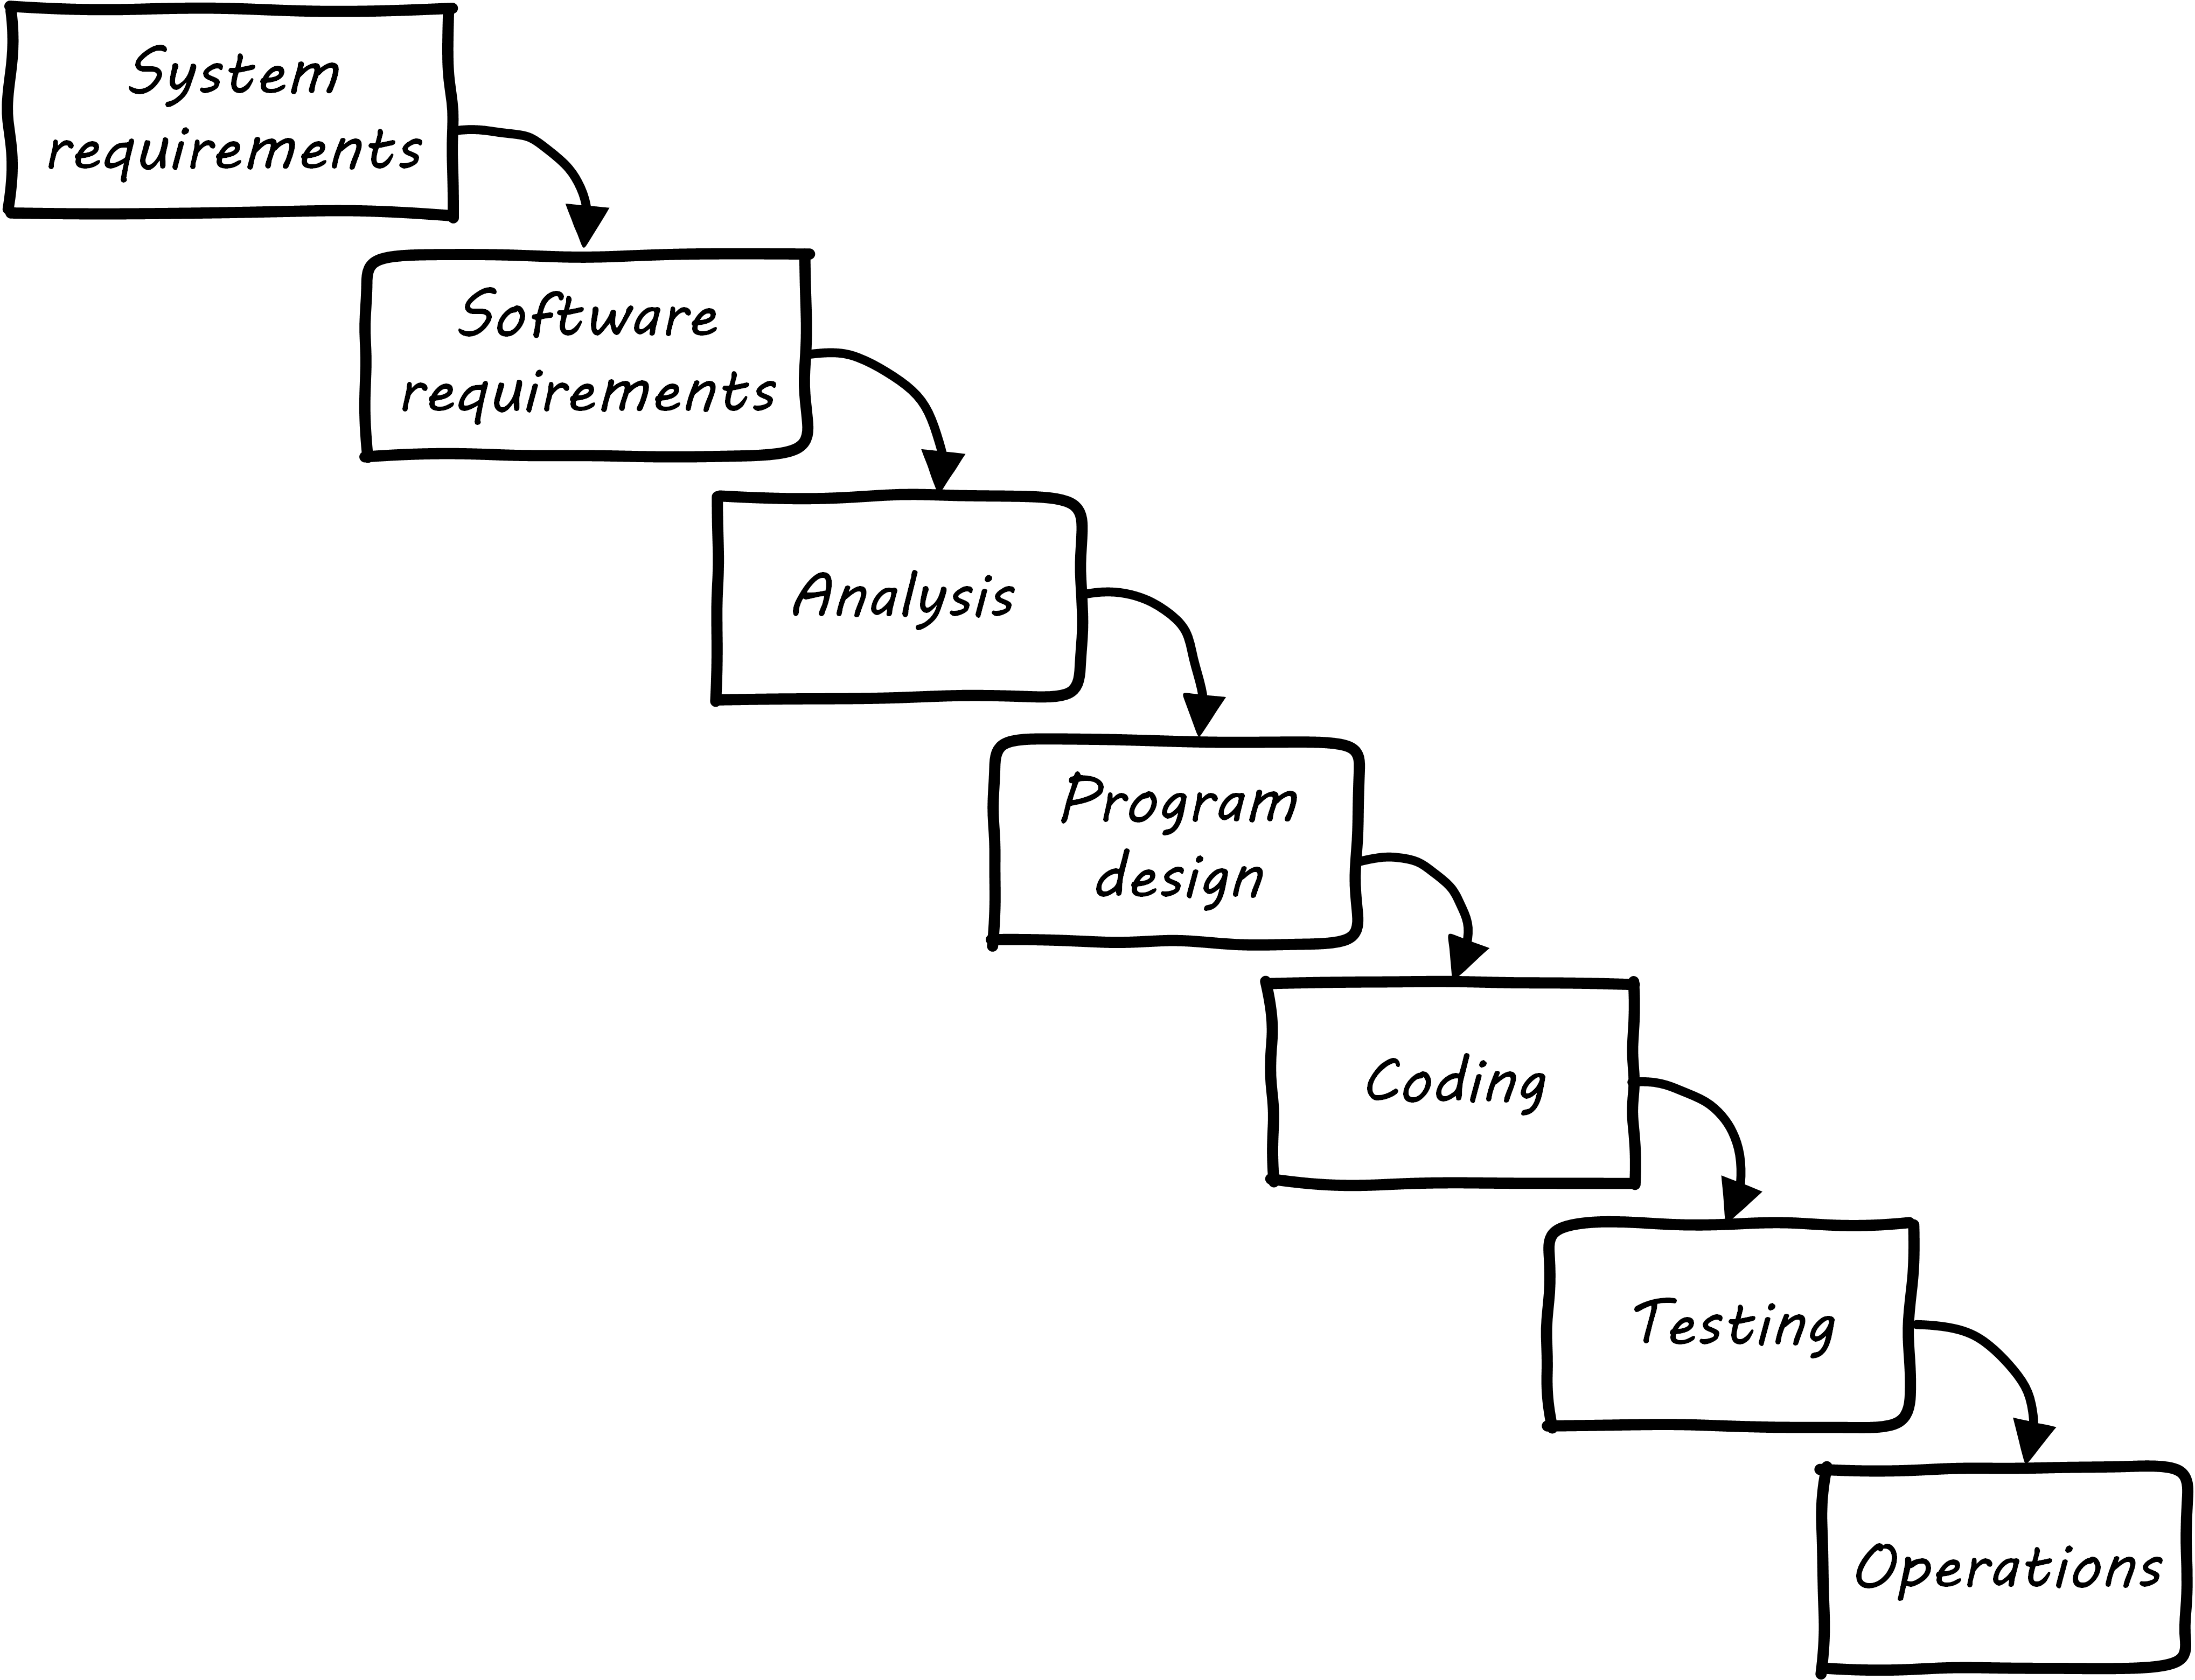
\includegraphics[width=0.48\textwidth]{images/1_03-waterfall.png}}}}{waterfall progression}
\end{center}
\caption[{Waterfall lifecycle }]{Waterfall lifecycle \footnotemark{}}
\end{wrapfigure}
 
First, requirements need to be extensively captured and analyzed before the work of development should commence. So, the project team would develop enormous spreadsheets of requirements, spending weeks on making sure that they represented what \textquotedblleft{}the customer\textquotedblright{} wanted. The objective was to get the customer's signature. Any further alterations could be profitably billed as \textquotedblleft{}change requests."
 
The analysis phase was used to develop a more structured understanding of the requirements, e.g. conceptual and logical data models, process models, business rules, and so forth.
 
In the design phase, the actual technical platforms would be chosen; major subsystems determined with their connection points, initial capacity analysis (\emph{volumetrics}) translated into system sizing, and so forth. (Perhaps hardware would not be ordered until this point, leading to issues with developers now being \textquotedblleft{}ready\textquotedblright{}, but hardware not being available for weeks or months yet).
 
Only AFTER extensive requirements, analysis, and design would coding take place (implementation). Furthermore, there were separation of duties between developers and testers. Developers would write code and testers would try to break it, filing bug reports that the developers would then need to respond to.
 
Another model sometimes encountered at this time was the V-{}model. This was intended to better represent the various levels of abstraction operating in the systems delivery activity. Requirements operate at various levels, from high level business intent through detailed specifications. It is all too possible that a system is \textquotedblleft{}successfully\textquotedblright{} implemented at lower levels of specification, but fails to satisfy the original higher level intent.
 \begin{wrapfigure}{r}{0.5\textwidth}[H]

\begin{center}
\imgexists{images/1_03-vmodel.png}{{\imgevalsize{images/1_03-vmodel.png}{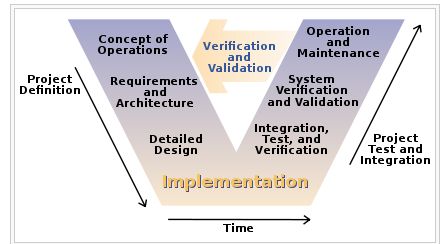
\includegraphics[width=0.48\textwidth]{images/1_03-vmodel.png}}}}{v-{}model}
\end{center}
\caption[{V-{}model }]{V-{}model \footnotemark{}}
\end{wrapfigure}
 
The failures of these approaches at scale are by now well known. Large distributed teams would wrestle with thousands of requirements. The customer would \textquotedblleft{}sign off\textquotedblright{} on multiple large binders, with widely varying degrees of understanding of what they were agreeing to. Documentation became an end in itself, and yet did not meet its objectives of ensuring continuity if staff turned over. The development team would design and build extensive product implementations without checking the results with customers. They would also defer testing that various component parts would effectively interoperate until the very end of the project, when the time came to assemble the whole system.
 
Failure after failure of this approach is apparent in the historical record (\hyperlink{Glass1998}{[Glass1998]}). Recognition of such failures, dating from the 1960s, led to the perception of a \textquotedblleft{}software crisis.\textquotedblright{}  (It should also be noted that many large systems were effectively constructed and operated during the "waterfall years", and that there are reasonable criticisms of the concept of a \textquotedblleft{}software crisis\textquotedblright{} \hyperlink{Bossavit2015}{[Bossavit2015]}).
 
Successful development efforts existed back to the earliest days of computing (otherwise, we probably wouldn't have computers, or at least not so many). Many of these successful efforts used prototypes and other means of building understanding and proving out approaches. But highly publicized failures continued, and a substantial movement against \textquotedblleft{}waterfall\textquotedblright{} development started to take shape.
 
By the 1990s, a number of thought leaders in software development had noticed some common themes with what seemed to work and what didn't. Kent Beck developed a methodology known as \textquotedblleft{}eXtreme Programming,\textquotedblright{} or XP \hyperlink{Beck2000}{[Beck2000]}. XP pioneered the concepts of iterative, fast-{}cycle development with ongoing stakeholder feedback, coupled with test-{}driven development, ongoing refactoring, pair programming, and other practices. (More on the specifics of these in the next section.)
 
Various authors assembled in 2001 and developed the Agile Manifesto \hyperlink{Alliance2001}{[Alliance2001]}, which further emphasized an emergent set of values and practices:
 

\begin{sidebar}

\textbf{The Agile Manifesto} We are uncovering better ways of developing
software by doing it and helping others do it.
Through this work we have come to value:
\begin{itemize}

\item{} Individuals and interactions over processes and tools
 

\item{} Working software over comprehensive documentation
 

\item{} Customer collaboration over contract negotiation
 

\item{} Responding to change over following a plan
 
\end{itemize}

That is, while there is value in the items on
the right, we value the items on the left more.
\end{sidebar}
 
The Manifesto authors further stated:
 

\begin{sidebar}

We follow these principles:
\begin{itemize}

\item{} Our highest priority is to satisfy the customer
through early and continuous delivery
of valuable software.
 

\item{} Welcome changing requirements, even late in
development. Agile processes harness change for
the customer's competitive advantage.
 

\item{} Deliver working software frequently, from a
couple of weeks to a couple of months, with a
preference to the shorter timescale.
 

\item{} Business people and developers must work
together daily throughout the project.
 

\item{} Build projects around motivated individuals.
Give them the environment and support they need,
and trust them to get the job done.
 

\item{} The most efficient and effective method of
conveying information to and within a development
team is face-{}to-{}face conversation.
 

\item{} Working software is the primary measure of progress.
 

\item{} Agile processes promote sustainable development.
The sponsors, developers, and users should be able
to maintain a constant pace indefinitely.
 

\item{} Continuous attention to technical excellence
and good design enhances agility.
 

\item{} Simplicity\textemdash{}\hspace{0em}the art of maximizing the amount
of work not done\textemdash{}\hspace{0em}is essential.
 

\item{} The best architectures, requirements, and designs
emerge from self-{}organizing teams.
 

\item{} At regular intervals, the team reflects on how
to become more effective, then tunes and adjusts
its behavior accordingly.
 
\end{itemize}
\end{sidebar}
 
See \href{http://agilemanifesto.org/}{http://agilemanifesto.org/\-}.
 
The Agile models for developing software aligned with the rise of Cloud and Web-{}scale IT. As new customer-{}facing sites like Flickr, Amazon, Netflix, Etsy, and Facebook scaled to massive proportions, it become increasingly clear that waterfall approaches were incompatible with their needs. Because these systems were directly user-{}facing, delivering monetized value in fast-{}moving competitive marketplaces, they required a degree of responsiveness previously not seen in \textquotedblleft{}back-{}office\textquotedblright{} IT or military-{}aerospace domains (the major forms that large scale system development had taken to date). We will talk more of product-{}centricity and the overall DevOps movement in the next section.
 
This new world did not think in terms of large requirements specifications. Capturing a requirement, analyzing and designing to it, implementing it, testing that implementation, and deploying the result to the end user for feedback became something that needed to happen at speed, with high repeatability. Requirements "backlogs" were (and are) never "done," and increasingly were the subject of ongoing re-{}prioritization, without high-{}overhead project "change" barriers.
 
Web-{}based systems integrate the software development lifecycle tightly with operational concerns. The development of new functionality is moved rapidly into a user-{}facing state, as opposed to previous models where software development was more distant in time and personnel from operations staff. The sheer size and complexity of these systems required much more incremental and iterative approaches to delivery, as the system could never be taken offline for the "next major release" to be installed.
 
Software was moving more directly into an operational state, and developers and operators were part of the same economic concern (contract software development never gained favor in the Silicon Valley web-{}scale community). So, it was possible to start breaking down the walls between \textquotedblleft{}development\textquotedblright{} and \textquotedblleft{}operations,\textquotedblright{} and that is just what happened.
 
Because large scale systems are complex and unpredictable, it is understood that new features are never fully understood until they are deployed at scale to the real end user base. Therefore, large scale web properties also started to \textquotedblleft{}test in production\textquotedblright{} (more on this in Chapter 6) in the sense that they would deploy new functionality to only some of their users. Rather than trying to increase testing to better understand things before deployment, these new firms accepted a seemingly higher level of risk in exposing new functionality sooner. (Part of their belief is that it actually is lower risk, because the impacts are never fully understood in any event.)
 
\label{continuous-delivery}\hyperlabel{continuous-delivery}
  
\subsection{The DevOps challenge}
\label{_the_devops_challenge}\hyperlabel{_the_devops_challenge}%
  
Consider this inquiry by Mary and Tom Poppendieck (\hyperlink{Poppendieck2007}{[Poppendieck2007]}, p. 92):
 

\begin{sidebar}

\textbf{How long would it take your organization to deploy a change that involved one single line of code? Do you deploy changes at this pace on a repeat, reliable basis?}
\end{sidebar}
 
The implicit goal is that the organization should be able to change one line of code, and in fact might want to do so on an ongoing basis. There is deep Lean/Agile theory behind this goal, theory developed in reaction to the pattern of massive software failures that characterized IT in the first fifty years of its existence. (We'll discuss some of the systems theory, including the concept of feedback, in the introduction to Part II and other aspects of Agile theory, including the ideas of Lean Product Development, in Parts II and III.)
 
Achieving this goal is feasible but requires new approaches. Various practitioners have explored this problem, with great success. Key initial milestones included:
 \begin{itemize}

\item{} The establishment of \textquotedblleft{}test-{}driven development\textquotedblright{} as a key best practice in creating software \hyperlink{Beck2000}{[Beck2000]}
 

\item{} Duvall's book \textquotedblleft{}Continuous Integration\textquotedblright{} \hyperlink{Duvall2007}{[Duvall2007]}
 

\item{} Allspaw \& Hammonds's seminal \href{http://www.slideshare.net/jallspaw/10-deploys-per-day-dev-and-ops-cooperation-at-flickr}{\textquotedblleft{}10 Deploys a Day\textquotedblright{}} presentation describing Etsy \hyperlink{Allspaw2009}{[Allspaw2009]}.
 

\item{} Humble \& Farley's \textquotedblleft{}Continuous Delivery\textquotedblright{} \hyperlink{Humble2011}{[Humble2011]}.
 
\end{itemize}
 
"DevOps" is a broad term, encompassing product management, team behaviors, and culture. At an execution level, the fundamental goal of moving smaller changes more quickly through the pipeline is a common theme. Other guiding principles include, "If it hurts, do it more frequently." (This is in part a response to the poor practice, or \emph{antipattern}, of deferring integration testing and deployment until those tasks are so big as to be unmanageable.) There is a great deal written on the topic of DevOps currently; the Humble/Farley book is recommended  as an introduction. Let's go into a little detail on some essential Agile/DevOps practices.
 \begin{itemize}

\item{} Test driven development
 

\item{} Ongoing refactoring
 

\item{} Continuous integration
 

\item{} Continuous deployment
 
\end{itemize}
 
In our scenario approach, at the end of the last chapter, you had determined a set of tools for creating your new IT-{}based product:
 \begin{itemize}

\item{} Development stack (language, framework, and associated enablers such as database and application server)
 

\item{} Cloud provider that supports your stack
 

\item{} Version control
 

\item{} Deployment capability
 
\end{itemize}
 
You'll be creating text files of some sort, and almost certainly importing various additional libraries, packages, modules, etc, rather than solving problems others have already figured out.
 \begin{DBKadmonition}{}{Note}
 
Development tools such as text editors and integrated development environments (IDEs) are out of scope for this book, as they are often matters of personal choice and limited to developers' desktops.
 \end{DBKadmonition}
 
The assumption in this chapter is that you are going to start IMMEDIATELY with a continuous delivery pipeline. \textbf{You want to set this up before developing a single line of code.} This is not something to "get around to later." It's not that difficult (see the online resources for further discussion and pointers to relevant open source projects). What is meant by a continuous delivery pipeline? Here is a simplified, starting overview, based on the \href{https://github.com/dm-academy/Calavera}{Calavera project} developed for the IT Delivery course at the University of St. Thomas:
 
\label{pipeline}\hyperlabel{pipeline}
 \begin{wrapfigure}{r}{0.5\textwidth}[H]

\begin{center}
\imgexists{images/1_03-pipeline.png}{{\imgevalsize{images/1_03-pipeline.png}{\includegraphics[width=0.48\textwidth]{images/1_03-pipeline.png}}}}{pipeline}
\end{center}
\caption{A simple continuous delivery toolchain}
\end{wrapfigure}
 \begin{enumerate}[label=\arabic*.]

\item{} First, some potential for value is identified. It is refined through product management techniques into a feature -{} some specific set of functionality that when complete will enable the value proposition (i.e. as a \href{http://dm-academy.github.io/aitm/#_it_services_systems_and_applications}{moment of truth}.)
 

\item{} The feature is expressed as some set of IT work, today usually in small increments lasting between 1 and 4 weeks (this of course varies). Software development commences, e.g. the creation of Java components by developers who first write tests, and then write code that satisfies the test.
 

\item{} The developer is continually testing the software as the build progresses, and keeping a local source control repository up to date with their changes at all times. When she or he reaches a level of satisfaction with the software, it is submitted to a centralized source repository.
 

\item{} When the repository detects the new "check-{}in," it contacts the build choreography manager, which launches a dedicated environment to build and test the new code. The environment is likely configured using \href{http://dm-academy.github.io/aitm/#_infrastructure_as_code}{infrastructure as code} techniques; in this way, it can be created automatically and quickly.
 

\item{} If the code passes all tests, the compiled and built binary executables may then be "checked in" to a package management repository.
 

\item{} From the package repository, the code may then be deployed to various environments, for further testing and ultimately to "production," where it can enable the consumer's value experiences.
 

\item{} Finally, the production system is monitored for availability and performance.
 
\end{enumerate}
 
We will discuss DevOps in terms of team behaviors and culture further in Chapter 7. For now, we stay closer to the tactical concerns of continuous delivery. Let's go into more detail on the major phases.
 
\label{system-intent}\hyperlabel{system-intent}
  
\subsection{Describing system intent}
\label{_describing_system_intent}\hyperlabel{_describing_system_intent}%
  
So, you've got an idea for a product value experience, and you have tools for creating it and infrastructure for running it. It's time to start building shippable product. As we will cover in more detail in the next chapter, the product development process starts with a concept of requirements (whether we call it story, use case, or scenario is not important). Requirements are numerous and evolving, and we're going to take some time looking at the process of converting them into IT-{}based functionality. There is history here back to the earliest days of computing.
 
In order to design and build a digital product, you need to express what you need the product to do. The conceptual tool used to do this is called Requirement.
The literal word \textquotedblleft{}Requirement\textquotedblright{} has fallen out of favor with the rise of Agile \hyperlink{Patton2014}{[Patton2014]}, and has a number of synonyms and variations:
 \begin{itemize}

\item{} Use case
 

\item{} User story
 

\item{} Nonfunctional requirement
 

\item{} Epic
 

\item{} Architectural epic
 

\item{} Architectural requirement
 
\end{itemize}
 
While these may differ in terms of focus and scope, the basic concept is the same -{} the requirement, however named, expresses some intent or constraint the system must fulfill. This intent calls for work to be performed.
 

\begin{sidebar}

\textbf{Sidebar: The troubled term "requirements"}

In earlier times, the concept of "requirements" was often used as an sort of defense mechanism. Statements would often be heard such as:

"We can't start building anything, we don't fully understand the requirements"

"We can't change the requirements now, we've started building! Make up your mind!"

"The product is a failure because the business kept changing their mind about the requirements."

While the term "requirements" is still used throughout much education and training, the student should be aware of this history, and the fact that many Agile practitioners discourage use of the term.

As Jeff Patton says, "\ldots{}\hspace{0em}I learned the word requirements actually means \emph{shut up}." \hyperlink{Patton2014}{[Patton2014]}, introduction.
\end{sidebar}
 
User Story Mapping is a well known approach \hyperlink{Patton2014}{[Patton2014]} with origins in the Scrum community. Here is an example from \hyperlink{Cohn2010}{[Cohn2010]}
 
"As a shopper, I can select how I want items shipped based on the actual costs of shipping to my address so that I can make the best decision."
 
The basic format is,
 
As a <{} type of user >{}, I want <{} goal >{}, so that <{} some value >{}.
 
The story concept is flexible, and can be aggregated and decomposed in various ways, as we will discuss in Chapter 4. Our interest here is in the basic stimulus for application development work that it represents.
 
You don't need an extensively automated system at this stage to capture requirements, but you need \textbf{something}. It could be a spreadsheet, or a shared word processing document, or sticky notes on a whiteboard (we'll talk about Kanban in the next section.) The important thing is to start somewhere, with team agreement as to what the approach is, so you can move forward collaboratively.
 
We will discuss approaches for "discovering" user stories and product features in Chapter 4, where Product Management is formalized. For now, as an early startup of one or two people, it is sufficient that you have some basic ability to characterize your system intent\hspace{0.167em}\textemdash{}\hspace{0.167em}more formalized techniques come later.
  
\subsection{Test-{}driven development and refactoring}
\label{_test_driven_development_and_refactoring}\hyperlabel{_test_driven_development_and_refactoring}%
  
Testing software and systems is a critically important part of digital product development. The earliest concepts of \hyperlink{Agile-history}{waterfall development} called for it explicitly, and "software tester" as a role and "software quality assurance" as a practice have long histories. Evolutionary approaches to software have a potential major issue with software testing:
 \begin{quote}

As a consequence of the introduction of new bugs, program maintenance requires far more system testing per statement written than any other programming. Theoretically, after each fix one must run the entire bank of test cases previously run against the system, to ensure that it has not been damaged in an obscure way.
In practice such regression testing must indeed approximate this theoretical ideal, and it is very costly.

\hspace*\fill--- Fred Brooks
\emph{Mythical Man-{}Month} \end{quote}
 
This issue was and is well known to thought leaders in Agile software development. The key response has been the concept of automated testing, so that any change in the software can be immediately validated before more development along those lines continues. One pioneering tool was JUnit:
 \begin{quote}

\emph{The reason JUnit is important . . . is that the presence of this tiny tool has been essential to a fundamental shift for many programmers. A shift where testing has moved to a front and central part of programming. People have advocated it before, but JUnit made it happen more than anything else.}

\hspace*\fill--- Martin Fowler
\emph{http://martinfowler.com/books/meszaros.html} \end{quote}
 
From the reality that regression testing was "very costly" (as stated by Brooks in the above quote), the emergence of tools like JUnit (coupled with increasing computer power and availability) changed the face of software development, allowing the ongoing evolution of software systems in ways not previously possible.
 
\subsubsection{Test-{}driven development}
\label{_test_driven_development}\hyperlabel{_test_driven_development}%
  
In test-{}driven development, the idea essence is to write code that tests itself, and in fact to \textbf{write the test before writing any code}. This is done through the creation of test harnesses and the tight association of tests with requirements. The logical culmination of test-{}driven development was expressed by Kent Beck in \emph{eXtreme Programming}: write the test first \hyperlink{Beck2000}{[Beck2000]}. Thus:
 \begin{enumerate}[label=\arabic*.]

\item{} Given a \textquotedblleft{}user story\textquotedblright{} (i.e \href{http://dm-academy.github.io/aitm/#_describing_system_intent}{system intent}), figure out a test that will demonstrate its successful implementation.
 

\item{} Write this test using the established testing framework.
 

\item{} Write the code that fulfills the test.
 
\end{enumerate}
 
Some readers may be thinking, \textquotedblleft{}I know how to write a little code, but what is this about using code to write a test?\textquotedblright{}
 
While we avoid much in-{}depth examination of source code in this book, using some simplified Java will help. Here is an example drawn from the  \href{https://github.com/CharlesTBetz/Calavera}{Calavera project}, the basis for the companion labs to this book.
 \begin{DBKadmonition}{warning}{Important}
 
Just read through the example carefully. You do not need to know Java.
 \end{DBKadmonition}
 
Let's say we want a function that will take a string of characters (e.g. a sentence) and wrap it in some \href{https://en.wikipedia.org/wiki/HTML}{HTML} \textquotedblleft{}Heading 1\textquotedblright{} tags. We will name the class \textquotedblleft{}H1Class\textquotedblright{} and (by convention) we will start by developing a class called TestH1Class.
 
We write the test first:
 
\begin{lstlisting}[firstnumber=1,backgroundcolor={},basicstyle=\ttfamily,]
public class TestClass1 {
 private H1Class a;  //
 @Before
 public void setUp() throws Exception {
  this.a = new H1Class("TestWebMessage");
 }
 @Test
  public void testTrue() {
    assertEquals("string correctly generated",
     "<h1>TestWebMessage</h1>",
     this.a.webMessage());// string built correctly
  }
}
\end{lstlisting}
 
The code above basically states,
 

\begin{sidebar}
\begin{enumerate}[label=\arabic*.]

\item{} Set up the object to be tested
 

\item{} pass in a message with the content "TestWebMessage"
 

\item{} the test passess if we get back "<{}h1>{}TestWebMessage<{}/h1>{}" -{} the original message surrounded by <{}h1>{} and <{}/h1>{} "tags," which are part of HTML.
 
\end{enumerate}
\end{sidebar}
 
We run the test (e.g. through Junit and Ant, which we won't detail here). It will fail. Then, we write the class:
 
\begin{lstlisting}[firstnumber=1,backgroundcolor={},basicstyle=\ttfamily,]
 public class H1Class {
  String strMsg;
  public String webMessage()
    {
      return "<h1>" + strMsg + "</h1>";
    }
}
\end{lstlisting}
 \begin{DBKadmonition}{warning}{Important}
 
These are simplified examples.
 \end{DBKadmonition}
 
When we run the test harness correctly (e.g. using a build tool such as Ant or Maven), the test class will perform the following actions:
 \begin{enumerate}[label=\arabic*.]

\item{} create an instance of the class H1Class, based on a string \textquotedblleft{}TestWebMessage\textquotedblright{}
 

\item{} confirm that the returned string is \textquotedblleft{}<{}h1>{}TestWebMessage<{}/h1>{}\textquotedblright{}
 
\end{enumerate}
 
If that string is not correctly generated, or the class cannot be created, or any other error occurs, the test fails and this is then reported via error results at the console, or (in the case of automated build) will be detected by the build manager and displayed as the build outcome. Other languages use different approaches from that shown here, but every serious platform at this point supports test-{}driven development.
 
The associated course lab provides a simple but complete example of a test-{}driven development environment, based on lightweight virtualization.
 
Employing test-{}driven development completely and correctly requires thought and experience. But it has emerged as a practice in the largest scale systems in the world. Google runs many millions of automated tests daily \hyperlink{Whittaker2012}{[Whittaker2012]}.  It has even been successfully employed in hardware development \hyperlink{Gruver2013}{[Gruver2013]}.
 
\label{refactoring}\hyperlabel{refactoring}
  
\subsubsection{Refactoring}
\label{_refactoring}\hyperlabel{_refactoring}%
  \begin{quote}

Refactoring is a controlled technique for improving the design of an existing code base. Its essence is applying a series of small behavior-{}preserving transformations, each of which is "too small to be worth doing". However, the cumulative effect of each of these transformations is quite significant. By doing them in small steps you reduce the risk of introducing errors. You also avoid having the system broken while you are carrying out the restructuring -{} which allows you to gradually refactor a system over an extended period of time.

\hspace*\fill--- Martin Fowler
\emph{Refactoring -{}-{} http://refactoring.com/} \end{quote}
 
\label{technical-debt-1}\hyperlabel{technical-debt-1}
 
Test-{}driven development enables the next major practice, that of refactoring. Refactoring is how you address technical debt. What is technical debt? Technical debt is a term coined by Ward Cunningham, and is now defined by Wikipedia as
 
\emph{\ldots{}the eventual consequences of poor system design, software architecture or software development within a codebase. The debt can be thought of as work that needs to be done before a particular job can be considered complete or proper. If the debt is not repaid, then it will keep on accumulating interest, making it hard to implement changes later on\ldots{}\hspace{0em} Analogous to monetary debt, technical debt is not necessarily a bad thing, and sometime technical debt is required to move projects forward.} \hyperlink{Wikipedia2016}{[Wikipedia2016]}
 
Test driven development ensures that the system's functionality remains consistent, while refactoring provides a means to address technical debt as part of ongoing development activities. Prioritizing the relative investment of repaying technical debt versus developing new functionality will be examined in future sections, but at least you now know the tools and concepts.
 
We discuss technical debt further in \hyperlink{technical-debt}{Chapter 12}.
   
\subsection{Continuous integration}
\label{_continuous_integration}\hyperlabel{_continuous_integration}%
  
\subsubsection{Version control, again: branching and merging}
\label{_version_control_again_branching_and_merging}\hyperlabel{_version_control_again_branching_and_merging}%
  \begin{quote}

Oddly enough, it seems that when you run into a painful activity, a good tip is to do it more often.

\hspace*\fill--- Martin Fowler
\emph{Foreword to Continuous Integration} \end{quote}
 
As systems engineering approaches transform to \hyperlink{cloud}{Cloud} and \hyperlink{infracode}{Infrastructure as Code}, a large and increasing percentage of IT work takes the form of altering text files and tracking their \hyperlink{version-control}{versions}. We have seen this in the previous chapter, with artifacts such as \hyperlink{infra-code-example}{scripts} being created to drive the provisioning and configuring of computing resources. Approaches which encourage ongoing development and evolution are increasingly recognized as less risky, since systems do not respond well to big "batches" of change. An important concept is that of "continuous integration,\textquotedblright{} popularized by Paul Duvall in his book of the same name \hyperlink{Duvall2007}{[Duvall2007]}.
 \begin{wrapfigure}{r}{0.5\textwidth}[H]

\begin{center}
\imgexists{images/1_03-dual-access.png}{{\imgevalsize{images/1_03-dual-access.png}{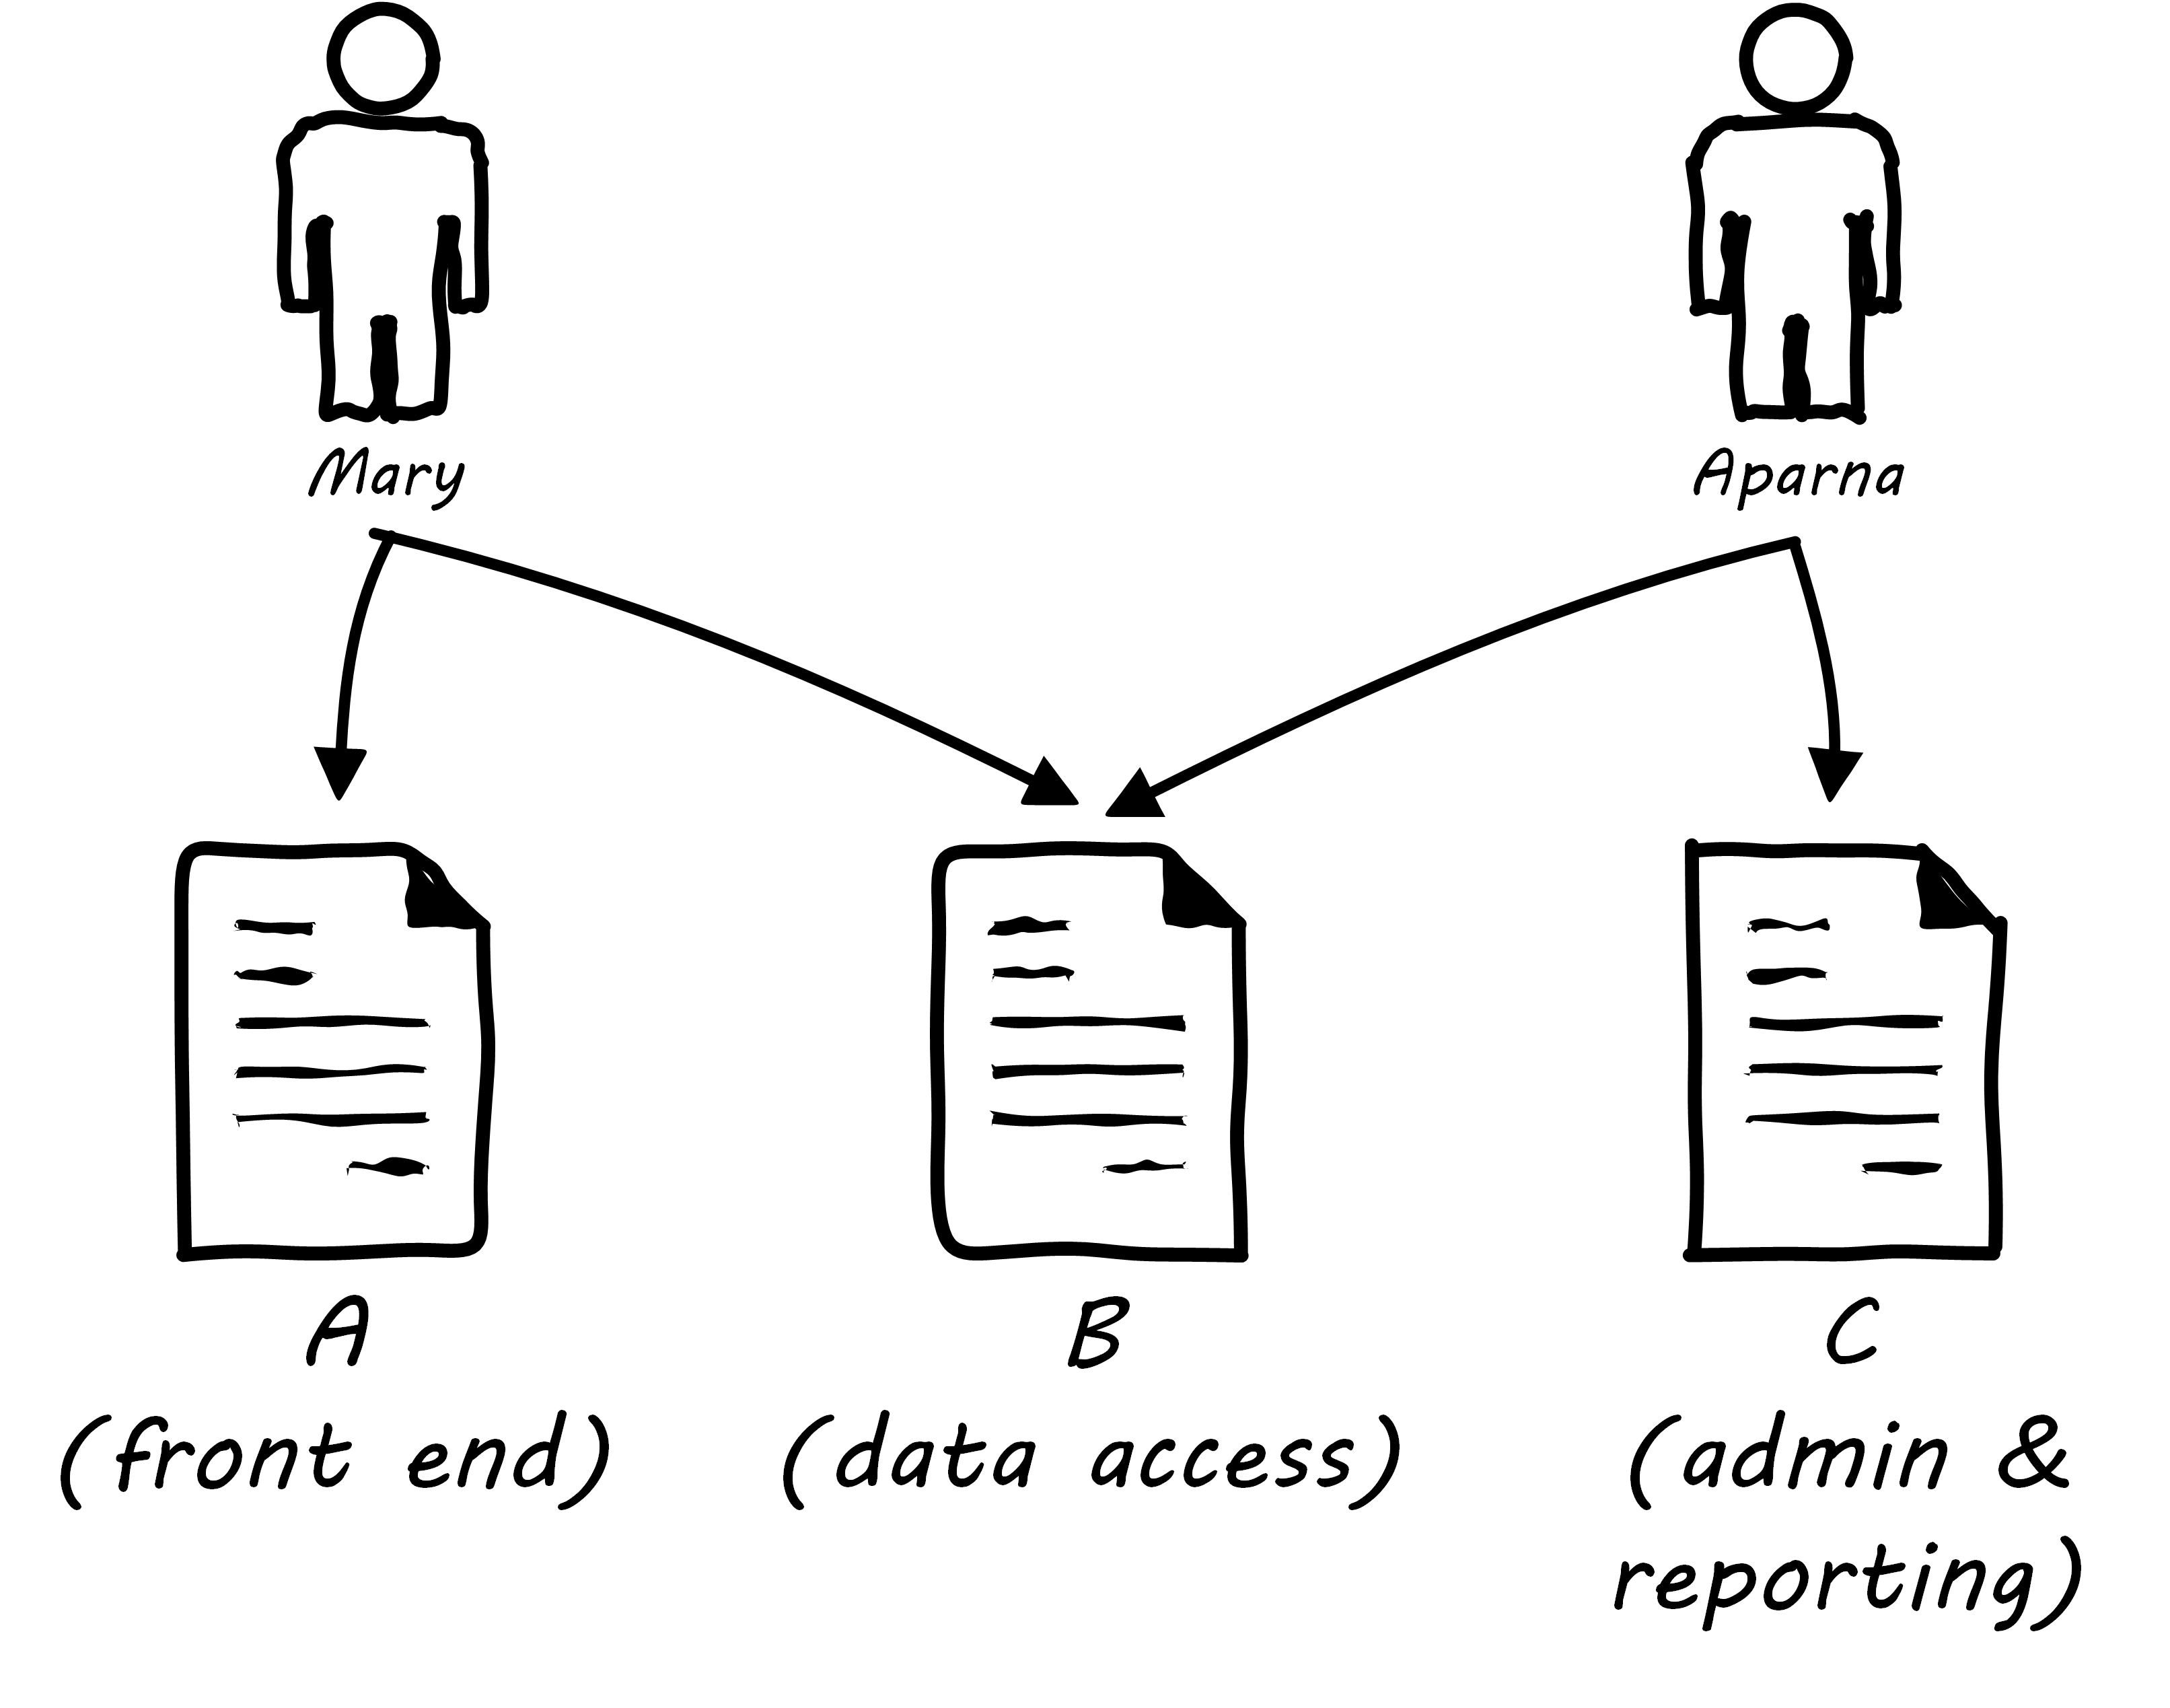
\includegraphics[width=0.48\textwidth]{images/1_03-dual-access.png}}}}{2 devs 3 files}
\end{center}
\caption{Two developers, one file}
\end{wrapfigure}
 
In order to understand why continuous integration is important, it is necessary to further discuss the concept of source control and how it is employed in real world settings. Imagine Mary have been working for some time with her partner Aparna in their startup (or on a small team) and they have three code modules. Mary is writing the web front end (file A), Aparna is writing the administrative tools and reporting (file C), and they both partner on the data access layer (file B). The conflict of course arises on the file B that they both need to work on.  A and C are mostly independent of each other, but changes to any part of B can have an impact on both their modules.
 
If changes are frequently needed to B, and yet they cannot split it into logically separate modules, they have a problem; they cannot both work on the same file at the same time. They are each concerned that the other does not introduce changes into B that \textquotedblleft{}break\textquotedblright{} the code in their own modules A and C.
 \begin{DBKadmonition}{}{Note}
 
Breaking a system apart by "layer" (e.g. front end versus data access) does not scale well. Microservices approaches encourage keeping data access and business logic together in functionally cohesive units. More on this in future chapters. But in this example, both developers are on the same small team. It is not always possible (or worth it) to divide work to keep two people from ever needing to change the same thing.
 \end{DBKadmonition}
 \begin{wrapfigure}{r}{0.5\textwidth}[H]

\begin{center}
\imgexists{images/1_03-dual-vc.png}{{\imgevalsize{images/1_03-dual-vc.png}{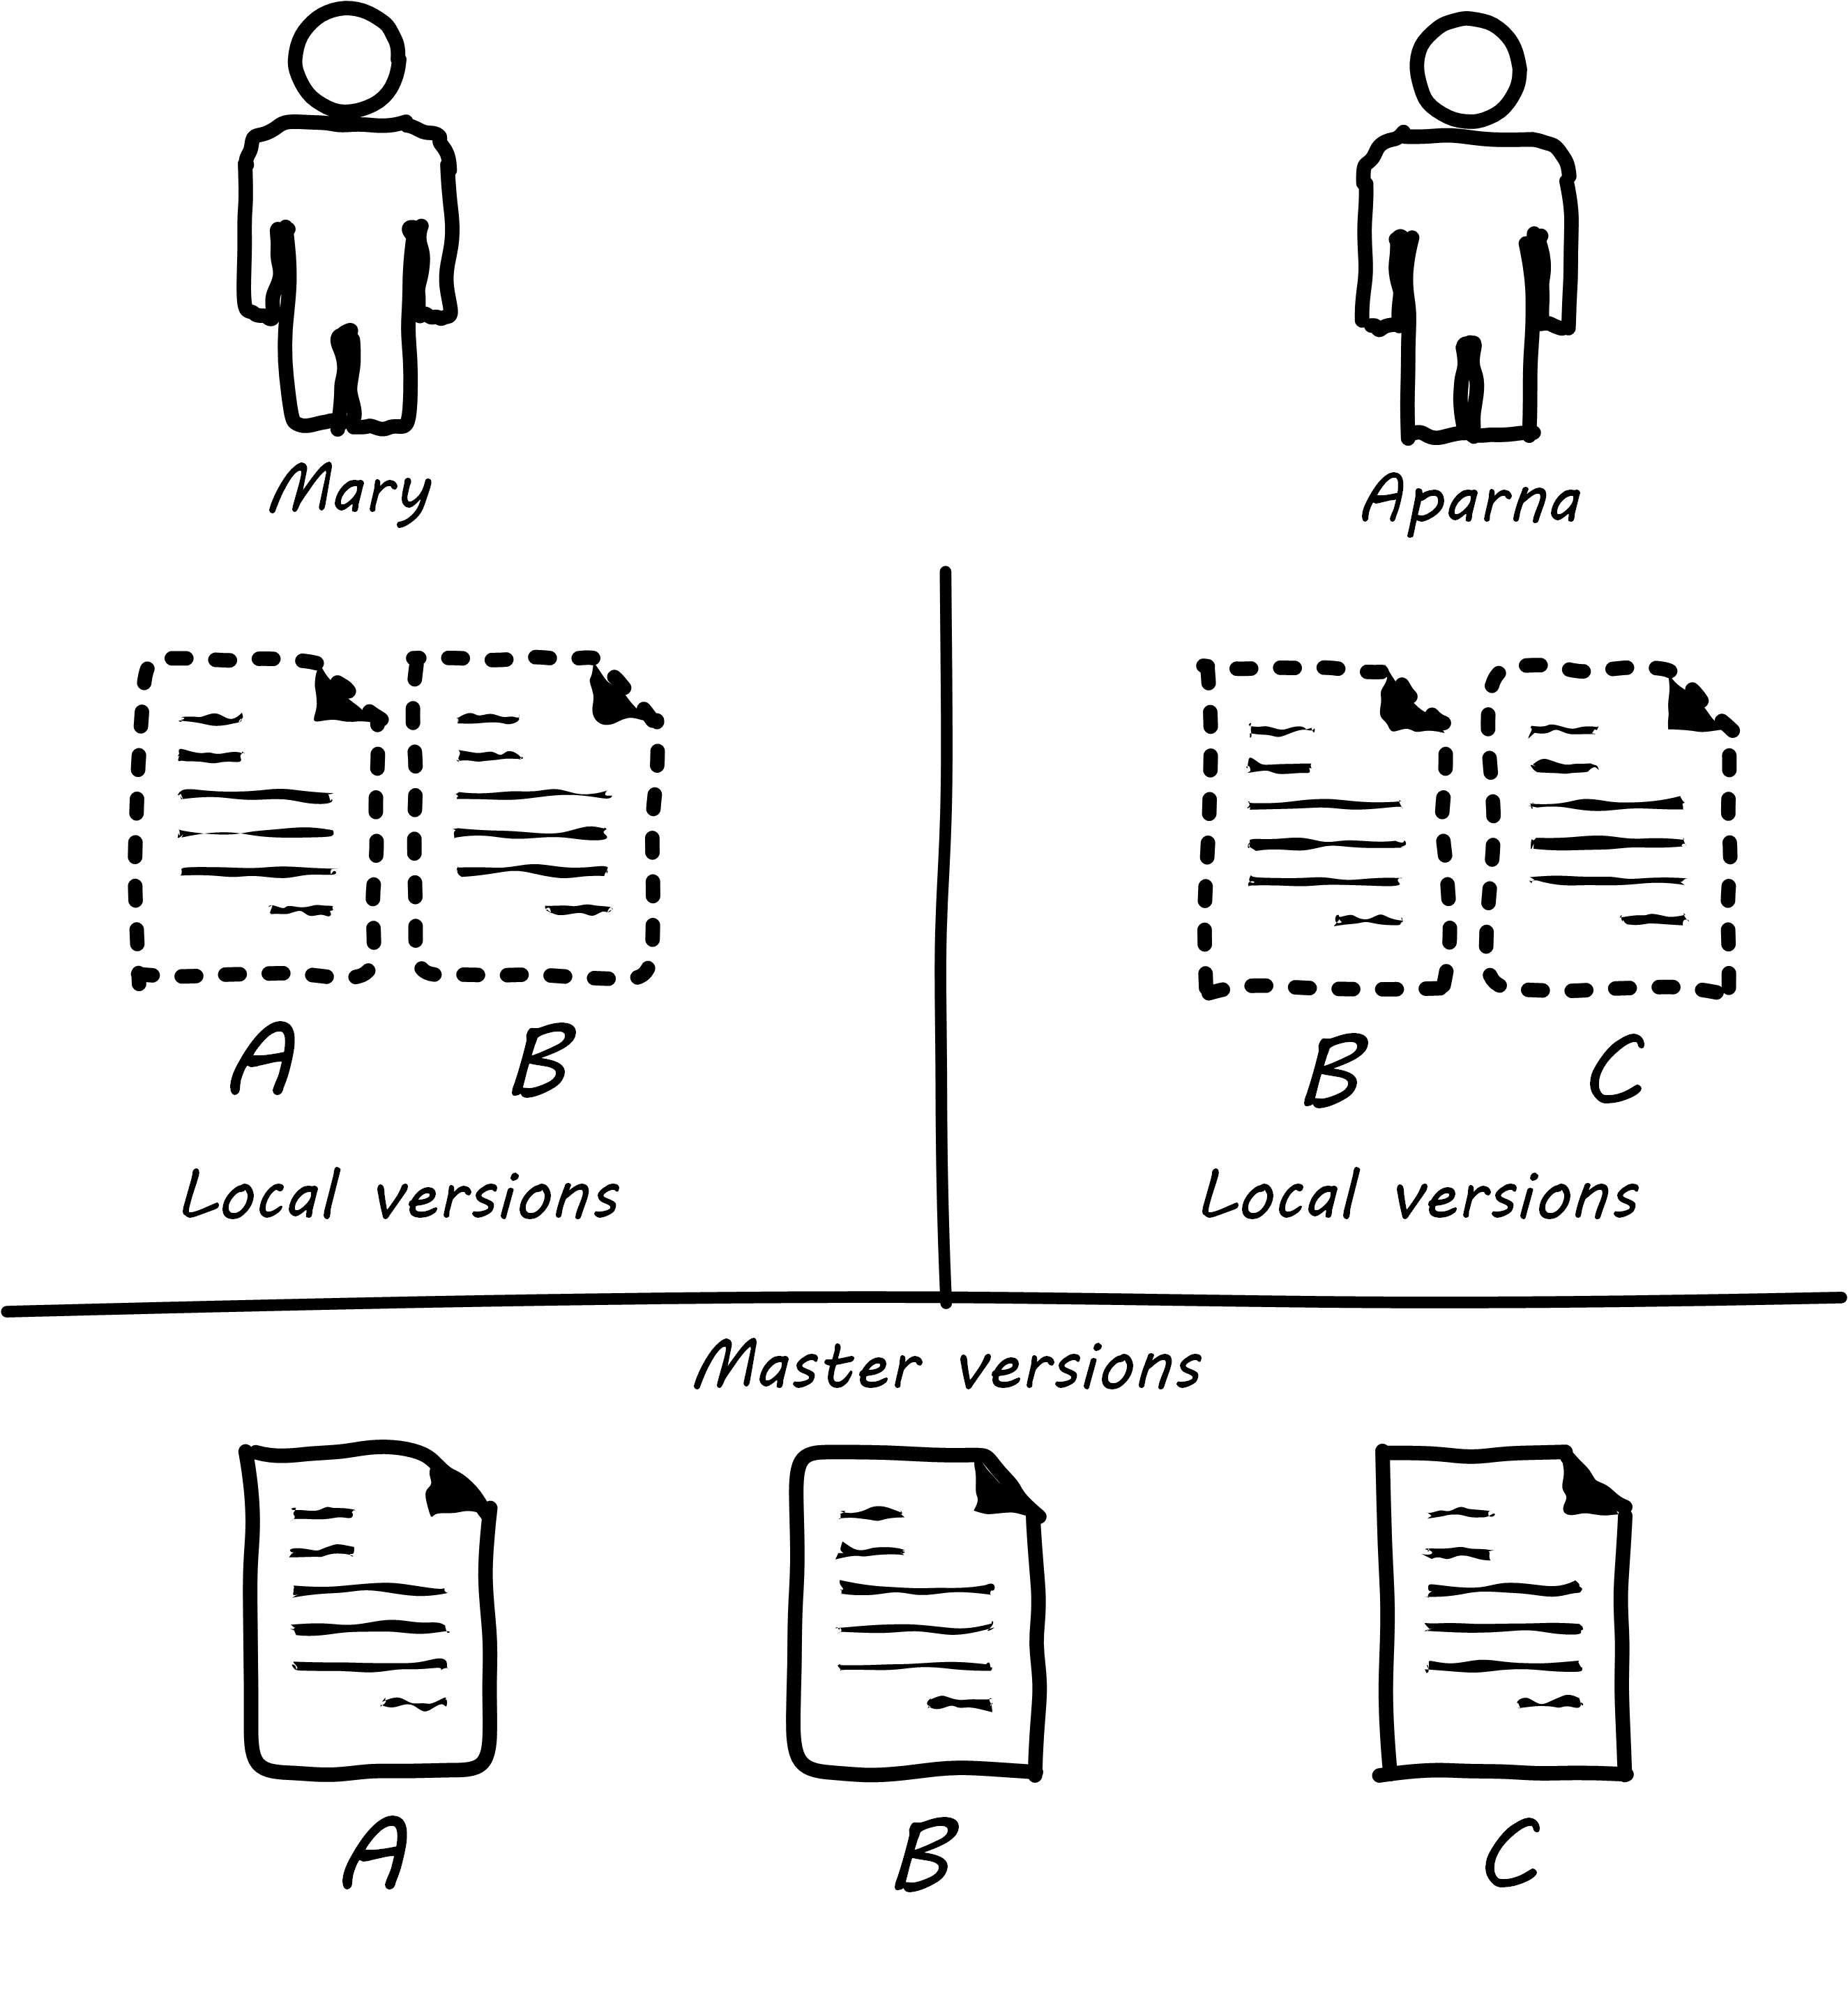
\includegraphics[width=0.48\textwidth]{images/1_03-dual-vc.png}}}}{2 devs on same file}
\end{center}
\caption{File B being worked on by 2 people}
\end{wrapfigure}
 
In smaller environments, or under older practices, perhaps there is no conflict, or perhaps they can agree to take turns. But even if they are taking turns, Mary still needs to test her code in A to make sure it's not been broken by changes Aparna made in B. And what if they really both need to work on B at the same time?
 
Now, because they took this book's advice and didn't start developing until they had \hyperlink{version-control}{version control} in place, each of them works on a "local" copy of the file (see illustration "File B being worked on by 2 people").
 
That way, they can move ahead on their local workstations. But when the time comes to combine both of your work, they may find themselves in "merge hell." They may have chosen very different approaches to solving the same problem, and code may need massive revision to settle on one code base. For example, in the accompanying illustration, Mary's changes to B are represented by triangles and Aparna's are represented by circles. They each had a local version on their workstation for far too long, without talking to each other.
 
In the diagrams, we represent the changes graphically; of course, with real code, the different graphics represent different development approaches each person took. For example, Mary had certain needs for how errors were handled, while Aparna had different needs.
 \begin{wrapfigure}{r}{0.5\textwidth}[H]

\begin{center}
\imgexists{images/1_03-merge-hell.png}{{\imgevalsize{images/1_03-merge-hell.png}{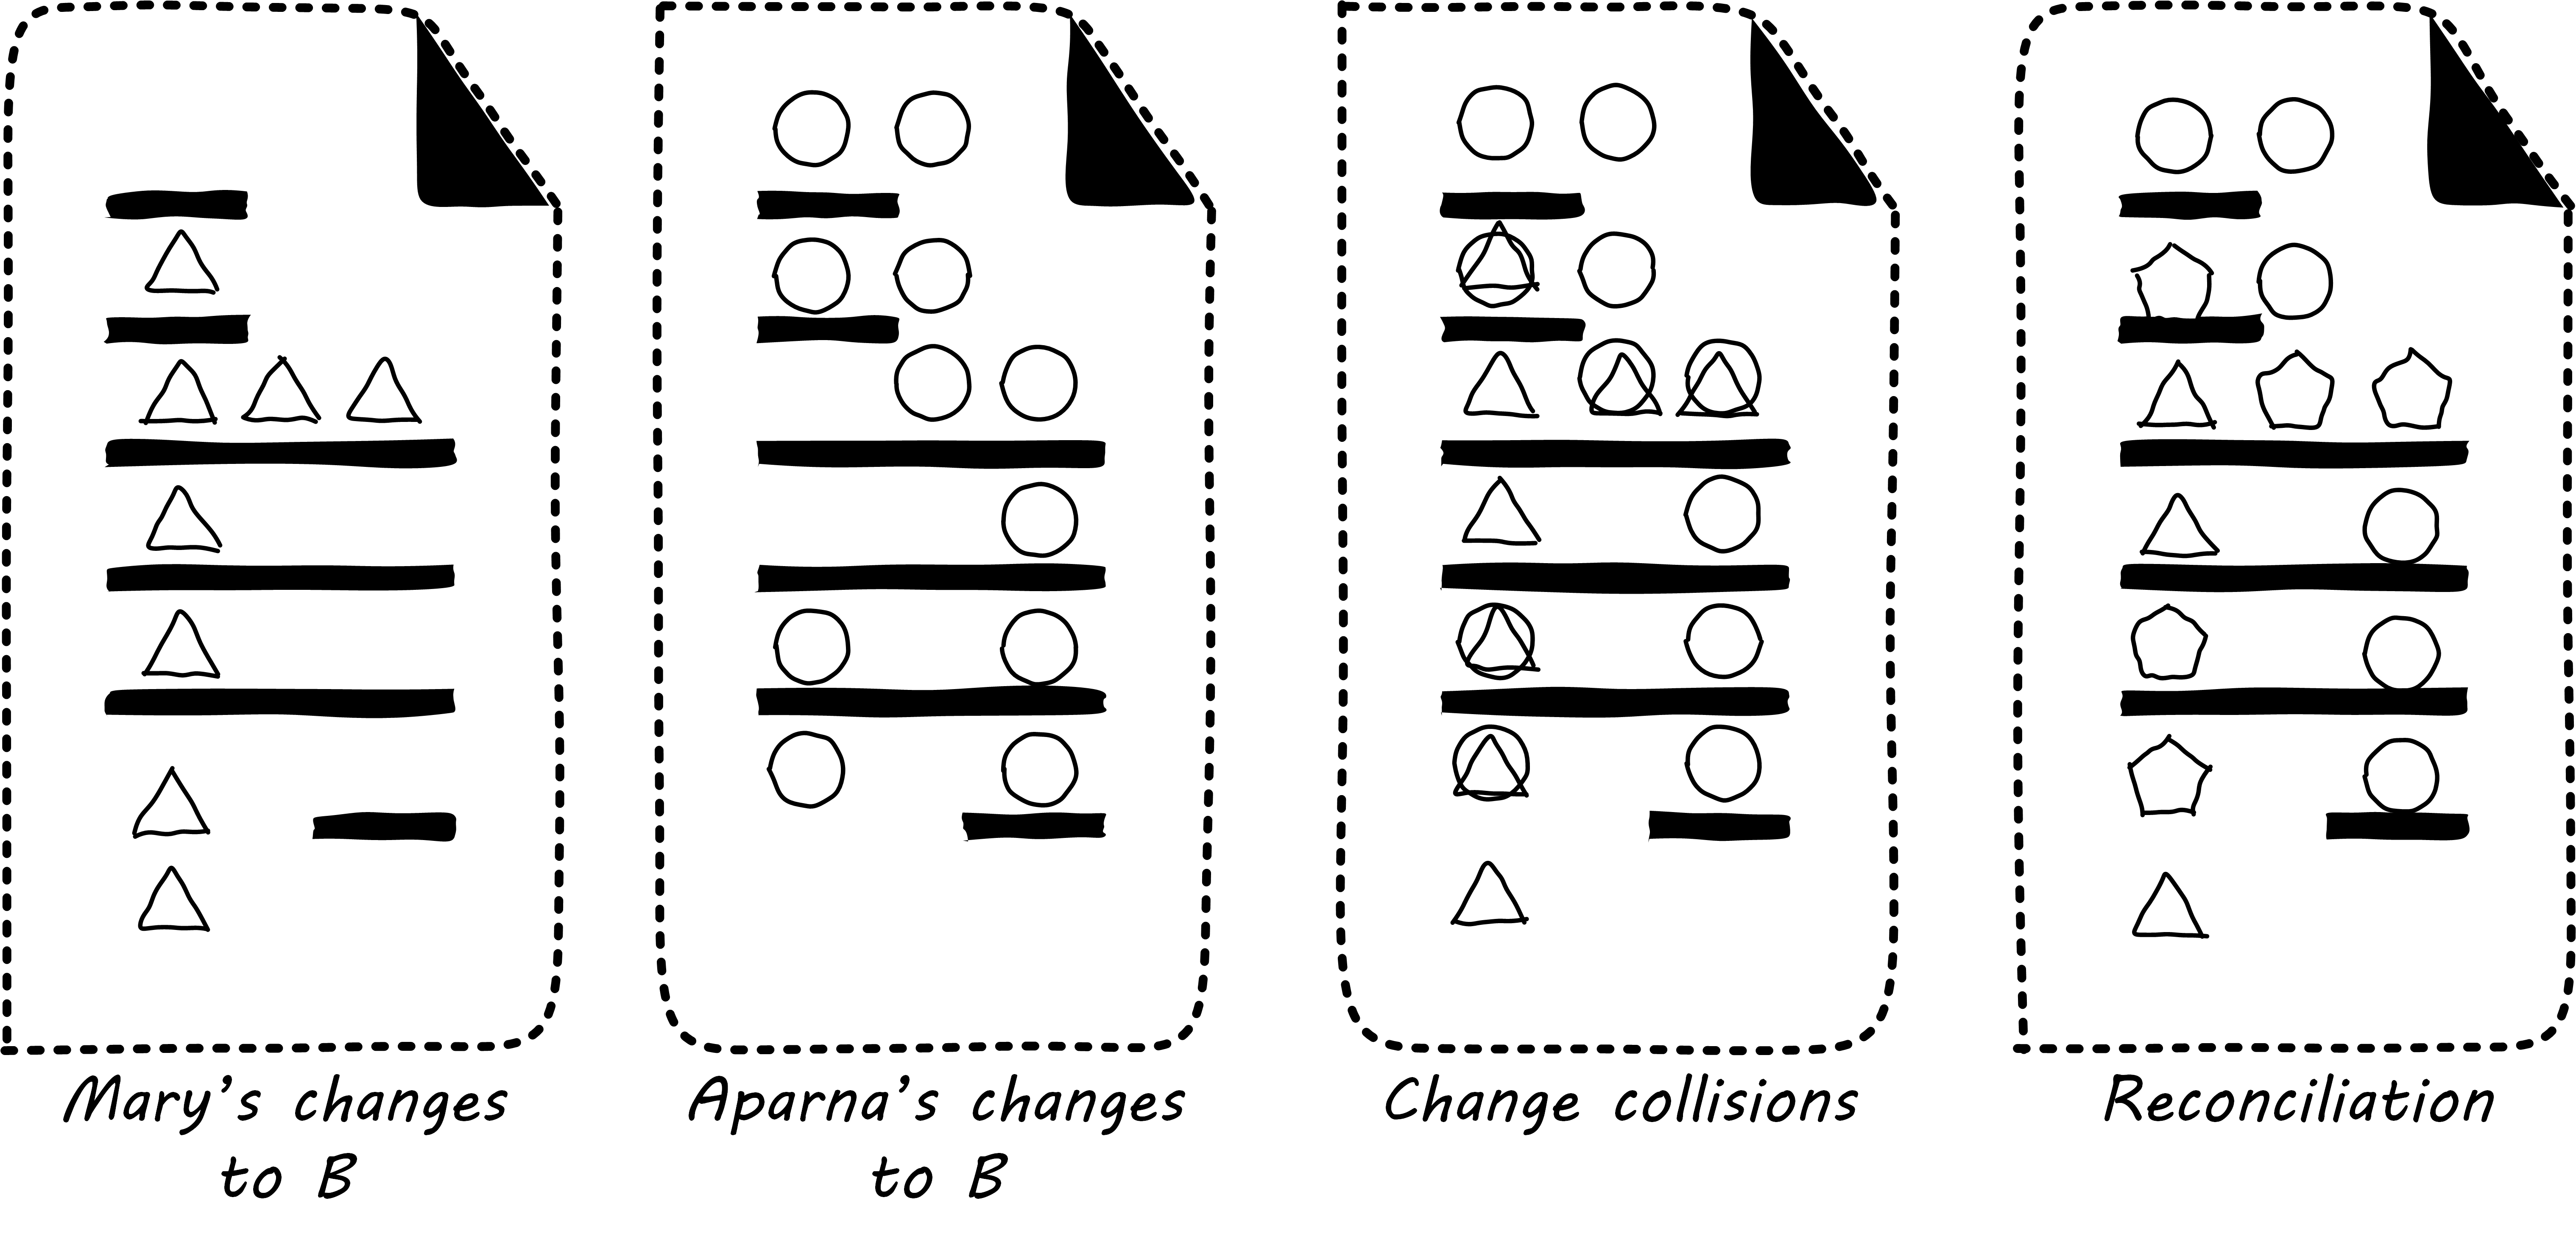
\includegraphics[width=0.48\textwidth]{images/1_03-merge-hell.png}}}}{merge hell}
\end{center}
\caption{Merge hell}
\end{wrapfigure}
 
In the diagram "Merge hell," where triangles and circles overlap, Mary and Aparna painstakingly have to go through and put in a consolidated error handling approach, so that the code supports both of their needs. The problem of course is now there are three ways errors are being handled in the code. This is not good, but they did not have time to go back and fix all the cases. This is a classic example of \hyperlink{technical-debt-1}{technical debt}.
 
Suppose instead that they had been checking in every day. They can identify the first collision quickly, and have a conversation about what the best error handling approach is. This saves them \textbf{both} the rework of fixing the collisions, \textbf{and} the technical debt they might have otherwise accepted:
 \begin{wrapfigure}{r}{0.5\textwidth}[H]

\begin{center}
\imgexists{images/1_03-fast-ID.png}{{\imgevalsize{images/1_03-fast-ID.png}{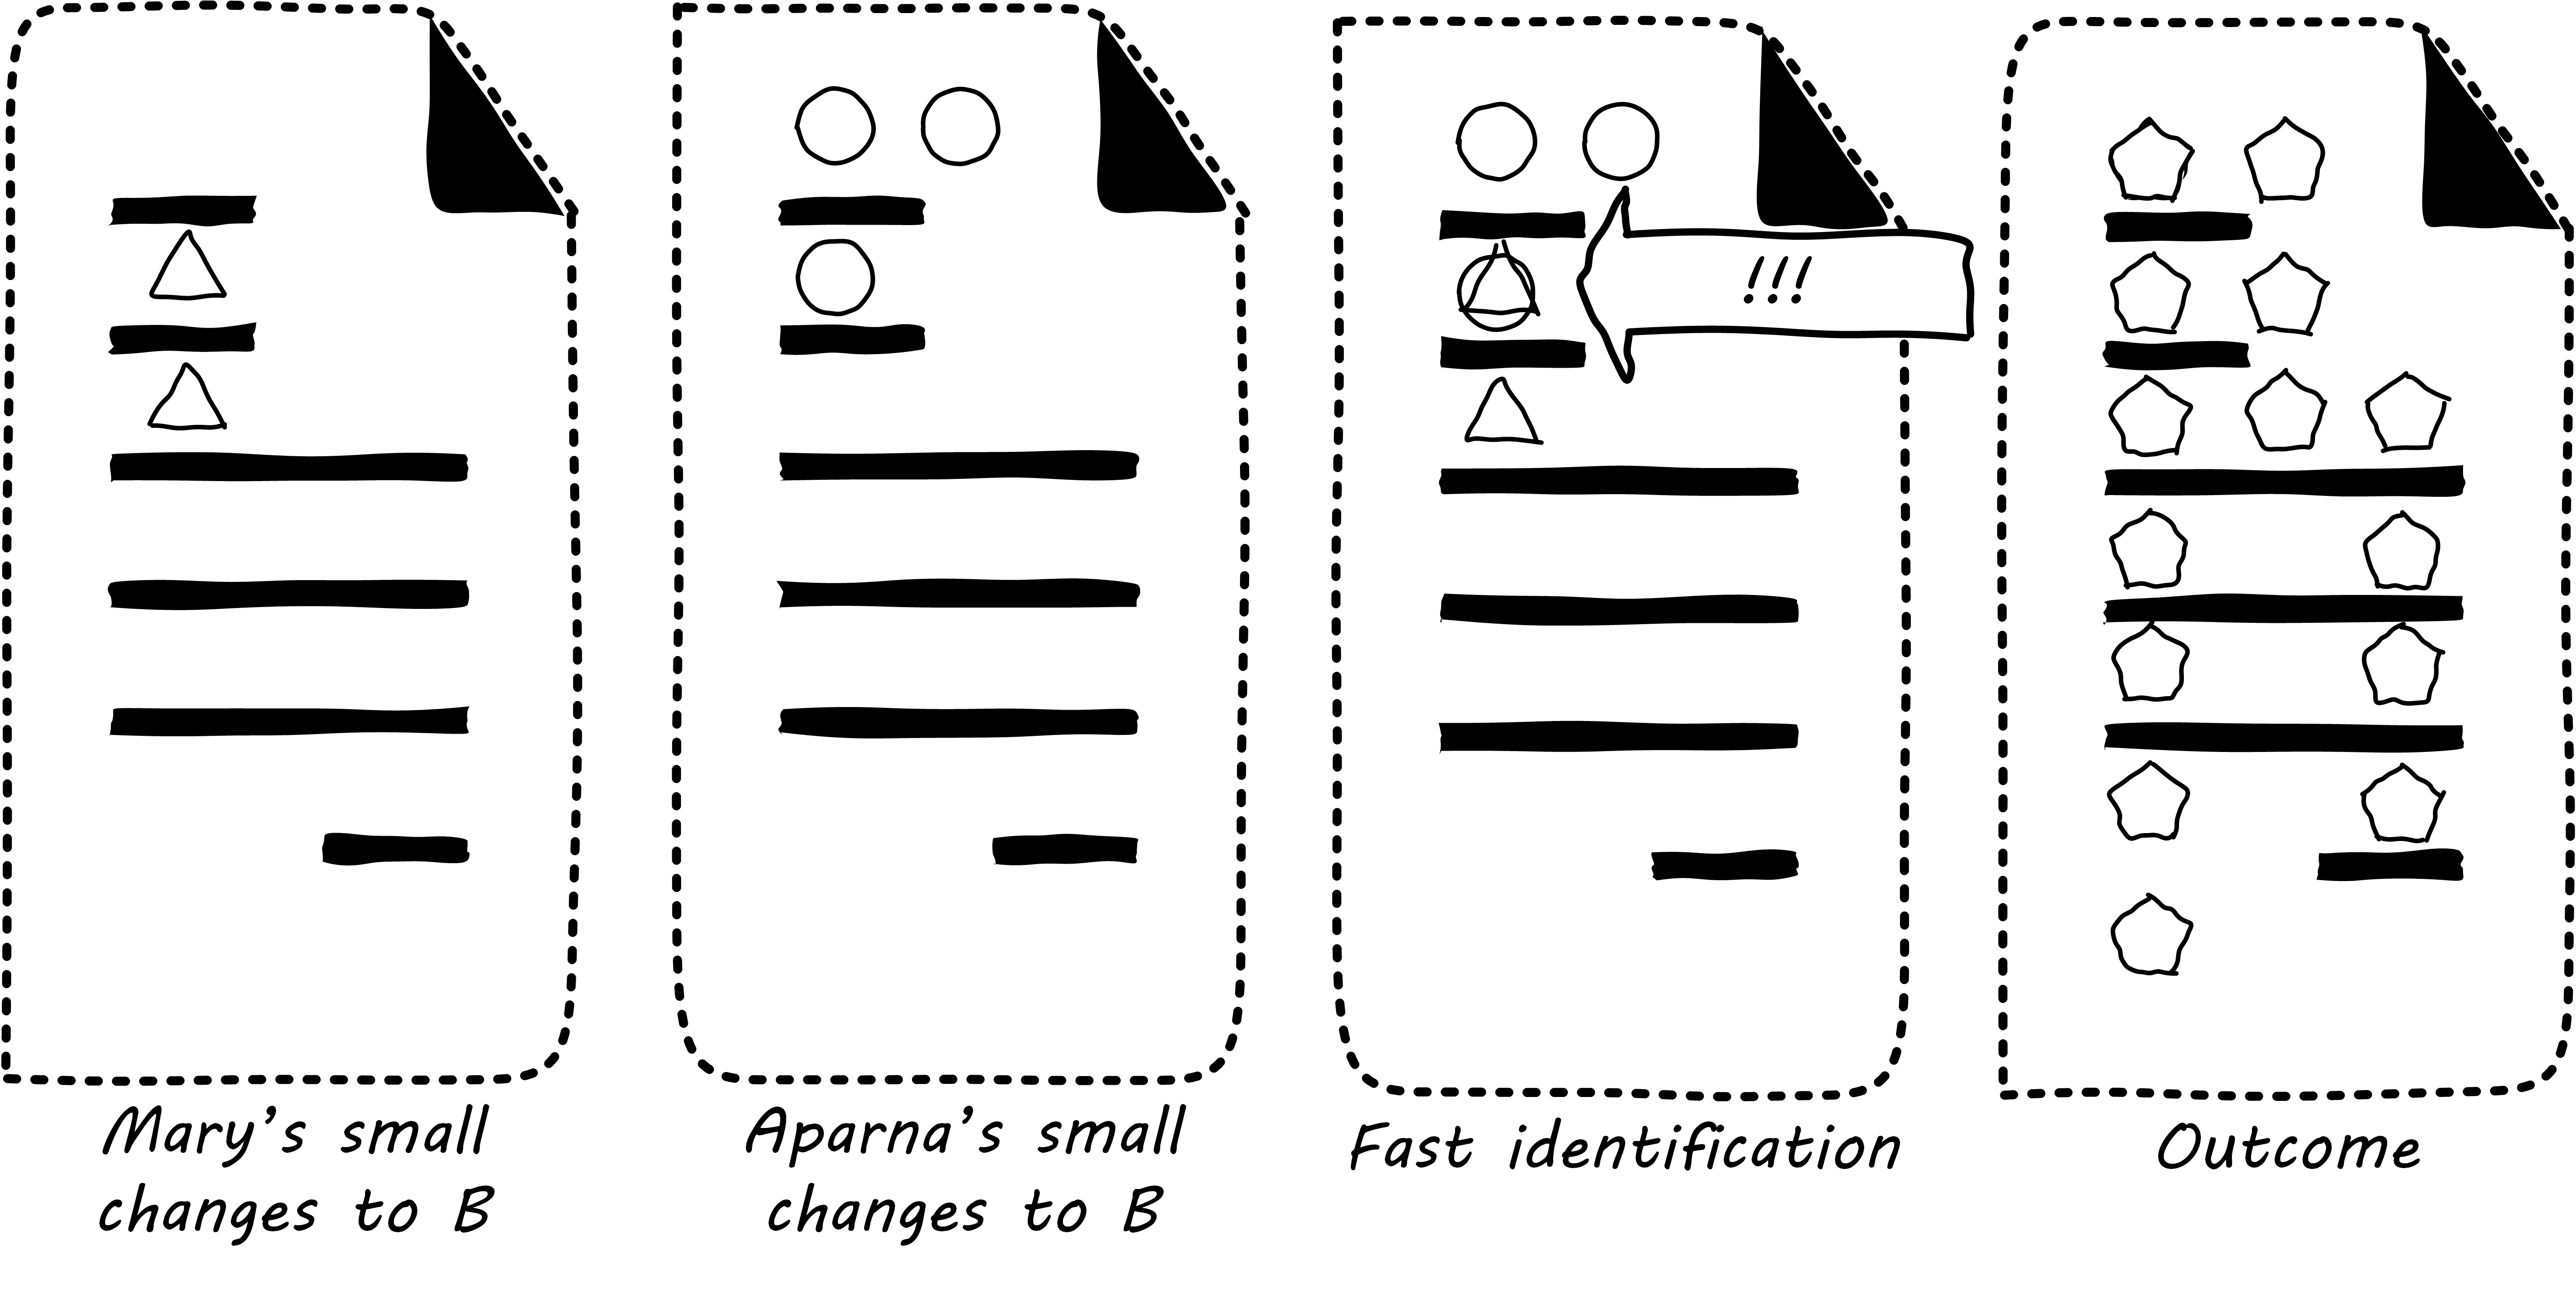
\includegraphics[width=0.48\textwidth]{images/1_03-fast-ID.png}}}}{errors caught quickly}
\end{center}
\caption{Catching errors quickly is valuable}
\end{wrapfigure}
 
These problems have driven the evolution of software configuration management for decades. In previous methods, to develop a new release, the code would be copied into a very long-{}lived "branch" (a version of the code to receive independent enhancement). Ongoing \textquotedblleft{}maintenance\textquotedblright{} fixes of the existing code base would also continue, and the two code bases would inevitably diverge. Switching over to the \textquotedblleft{}new\textquotedblright{} code base might mean that once-{}fixed bugs (bugs that had been addressed by maintenance activities) would show up again, and of course this would not be acceptable. So, when the newer development was complete, it would need to be merged back into the older line of code, and this was rarely if ever easy (again, "merge hell"). In a worst case scenario, the new development might have to be redone.
 
Enter continuous integration. As presented in \hyperlink{Duvall2007}{[Duvall2007]} the key practices (you will notice similarities to the \hyperlink{pipeline}{pipeline discussion}) include:
 \begin{itemize}

\item{} Developers run private builds including their automated tests before committing to source control
 

\item{} Developers check in to source control at least daily (hopefully we have been harping on this enough that you are taking it seriously by now).
 \begin{itemize}

\item{} Distributed version control systems such as git are especially popular, although older centralized products are \href{http://bitquabit.com/post/unorthodocs-abandon-your-dvcs-and-return-to-sanity/}{starting to adopt some of their functionality}
 

\item{} Integration builds happen several times a day or more on a separate, dedicated machine
 
\end{itemize}
 

\item{} 100\% of tests must pass for each build. Fixing failed builds is the highest priority.
 

\item{} A package or similar executable artifact is produced for functional testing
 

\item{} A defined package repository exists as a definitive location for the build output.
 
\end{itemize}
 
These practices are well developed and represent a highly evolved understanding gained through the painful trial and error of many development teams over many years. Rather than locking C so that only one person can work on it at a time, it's been found that the best approach is to allow developers to actually make multiple copies of such a file or file set and work on them simultaneously. Wait, you say. How can that work?
 
This is the principle of continuous integration at work. If the developers are continually pulling each other's work into their own working copies, and continually testing that nothing has broken, then distributed development can take place. So, if you are a developer, the day's work might be as follows:
 
8 AM: check out files from master source repository to a local branch on your workstation. Because files are not committed unless they pass all tests, you know that you are checking out clean code. You pull user story (requirement) that you will now develop.
 
8:30 AM: You define a test and start developing the code to fulfill it.
 
10 AM: You are closing in on wrapping up the first requirement. You check the source repository. Your partner has checked in some new code, so you pull it down to your local repository. You run all the automated tests and nothing breaks, so you're fine.
 
10:30: You complete your first update of the day; it passes all tests on your workstation. You commit it to the master repository. The master repository is continually monitored by the build server, which takes the code you created and deploys it, along with all necessary configurations, to a dedicated build server (which might be just a virtual machine or transient container). All tests pass there (the test you defined as indicating success for the module, as well as a host of older tests that are routinely run whenever the code is updated.
 
11:00: Your partner pulls your changes into their working directory. Unfortunately, some changes you made conflict with some work they are doing. You briefly consult and figure out a mutually acceptable approach.
 
Controlling simultaneous changes to a common file is only one benefit of continuous integration. When software is developed by teams, even if each team has its own artifacts, the system often fails to "come together" for higher-{}order testing to confirm that all the parts are working correctly together. Discrepancies are often found in the interfaces between components; when component A calls component B, it may receive output it did not expect and processing halts. Continuous integration ensures that such issues are caught early.
  
\subsubsection{Build choreography}
\label{_build_choreography}\hyperlabel{_build_choreography}%
  
Go back to the \hyperlink{pipeline}{pipeline picture} and consider step 4. While we discussed \hyperlink{version-control}{version control}, \hyperlink{package-mgmt}{package management}, and \hyperlink{deployment-mgmt}{deployment management} in Chapter 2, this is our first encounter with build choreography.
 
DevOps and continuous delivery call for automating everything that can be automated. This goal led to the creation of build choreography managers such as Hudson, Jenkins, Travis CI, and Bamboo. Build managers may control any or all of the following steps:
 \begin{itemize}

\item{} Detecting changes in version control repositories and building software in response
 

\item{} Alternately, building software on a fixed (e.g. nightly) schedule
 

\item{} Compiling source code and linking it to libraries
 

\item{} Executing automated tests
 

\item{} Combining compiled artifacts with other resources into installable packages
 

\item{} Registering new and updated packages in the package management repository, for deployment into downstream environments.
 

\item{} In some cases, driving deployment into downstream environments, including production. (This can be done directly by the build manager, or through the build manager sending a message to a \hyperlink{deployment-mgmt}{deployment management} tool.)
 
\end{itemize}
 
Build managers play a critical, central role in the modern, automated pipeline and will likely be a center of attention for the new digital professional in their career.
   
\subsection{Releasing software}
\label{_releasing_software}\hyperlabel{_releasing_software}%
  
\subsubsection{Continuous deployment}
\label{_continuous_deployment}\hyperlabel{_continuous_deployment}%
  
Once software is compiled and built, the executable files that can be installed and run operationally should be checked into a \href{https://en.wikipedia.org/wiki/Package_manager}{Package Manager}. At that point, one can take the last mile step and deploy the now tested and built software to pre-{}production or production environments. The software can undergo user testing, load testing, integration testing, and so forth. Once those tests are passed, it can be deployed to production.
 
(What is \textquotedblleft{}production,\textquotedblright{} anyway? We'll talk about environments in Section 2. For now, you just need to know that when an IT-{}based product is \textquotedblleft{}in production,\textquotedblright{} that means it is live and available to its intended base of end users or customers.)
 
Moving new code into production has always been a risky procedure. Changing a running system always entails some uncertainty. However, the practice of infrastructure as code coupled with increased virtualization has reduced the risk. Often, a rolling release strategy is employed so that code is deployed to small sets of servers while other servers continue to service the load. This requires careful design to allow the new and old code to co-{}exist at least for a brief time.
 
This is important so that the versions of software used in production are well controlled and consistent. The package manager can then be associated with some kind of deploy tool that keeps track of what versions are associated with which infrastructure.
 
Timing varies by organization. Some strive for true "continuous deployment," in which the new code flows seamlessly from developer commit through build, test, package and deploy. Others put gates in between the developer and check-{}in to mainline, or source to build, or package to deploy, so that some human governance remains in the toolchain. We will go into more detail on these topics in chapter 6.
 
\label{release-mgmt}\hyperlabel{release-mgmt}
  
\subsubsection{The concept of "release"}
\label{_the_concept_of_release}\hyperlabel{_the_concept_of_release}%
  
Release management, and the concept of a "release," are among the most important and widely-{}seen concepts in all forms of digital management. Regardless of whether you are a cutting-{}edge Agile startup with 2 people, or one of the largest banks with a portfolio of thousands of applications, you will likely be using releases for coordination and communication.
 
What is a "release?" I have defined it this way in other work: "A significant evolution in an IT service, often based on new systems development, coordinated
with affected services and stakeholders." Release management's role is to "Coordinate the assembly of IT functionality into a coherent whole and deliver this package Into a state in which the customer is getting the
intended value."  (\hyperlink{Betz2011a}{[Betz2011a]}, pp. 68, 119).
 
Even as a startup of 1, you know when your product is "ready for prime time" or not. Your first "release" should be a cause for some celebration: you now are offering digital value to some part of the world.
 
We will talk much more of release management in Parts II and III. At this point, you may not see it as much different from simply deploying, but even at the smallest scale you start to notice that \textbf{some changes require more thought and communication than others.} Simple bugfixes, or self-{}explanatory changes to the product's interfaces, can flow through your pipeline. But if you are going to radically change the system\hspace{0.167em}\textemdash{}\hspace{0.167em}even if you only have one customer\hspace{0.167em}\textemdash{}\hspace{0.167em}you need to communicate with them about this. And so, the concept of release management becomes part of your world.
   
\subsection{Application development topics}
\label{_application_development_topics}\hyperlabel{_application_development_topics}%
  
\subsubsection{Application architecture}
\label{_application_architecture}\hyperlabel{_application_architecture}%
  \begin{wrapfigure}{r}{0.5\textwidth}[H]

\begin{center}
\imgexists{images/1_03-sw-arch.jpg}{{\imgevalsize{images/1_03-sw-arch.jpg}{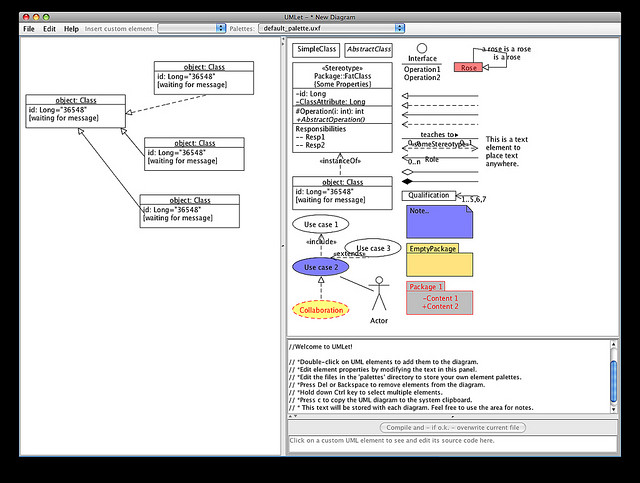
\includegraphics[width=0.48\textwidth]{images/1_03-sw-arch.jpg}}}}{software architecture}
\end{center}
\caption[{Software architecture tool }]{Software architecture tool \footnotemark{}}
\end{wrapfigure}
 
The design and architecture of applications is a large topic (see e.g. \hyperlink{Gamma1995}{[Gamma1995]} and \hyperlink{Fowler2003}{[Fowler2003]}) and this text only touches lightly on it. \href{http://www.iso-architecture.org/ieee-1471/defining-architecture.html}{ISO/\-IEC 41010} defines architecture as \textquotedblleft{}the fundamental organization of a system, embodied in its components, their relationships to each other and the environment, and the principles governing its design and evolution.\textquotedblright{}
 
A computer program can be as simple as \href{https://en.wikipedia.org/wiki/%22Hello,_World!%22_program}{Hello World.} Such a program requires only one or a few files to compile and execute. However, significant applications such as an online video streaming service require hardware and software configurations of \href{http://techblog.netflix.com/search/label/cloud%20architecture}{tremendous complexity}.  Specialized visual notations are used to describe this complexity, as in the image above. We will discuss this further in Chapter 12.
  
\subsubsection{Applications and project management}
\label{_applications_and_project_management}\hyperlabel{_applications_and_project_management}%
  
Because the initial applications were implemented as a kind of systems engineering, and were expensive to build and maintain, the technique of choice was \href{https://en.wikipedia.org/wiki/Project_management}{project management}. Project management will not be covered in this book until Part III, as it is not appropriate to the earlier stages of this book's \href{http://dm-academy.github.io/aitm/#_a_process_of_emergence}{emergence model}.
 
This history of project managed systems engineering produced any number of successes, but by the early 1990s there were significant concerns with the rate of large project failures \hyperlink{Glass1998}{[Glass1998]}, which occurred despite seemingly extensive and rigorous bureaucratic overhead, evidenced by frameworks such as \href{https://en.wikipedia.org/wiki/Capability_Maturity_Model_Integration}{CMMI} and \href{https://en.wikipedia.org/wiki/Project_Management_Body_of_Knowledge}{PMBOK}. \footnote{
Both project management and CMMI have come in for significant criticism \hyperlink{Koskela2002}{[Koskela2002]}, \hyperlink{Keefer2006}{[Keefer2006]}, and will be discussed further in Sections 3 and 4.
}
 
\emph{Second draft ideas}
 
\begin{lstlisting}[firstnumber=1,backgroundcolor={},basicstyle=\ttfamily,]
QA beyond test driven development - big oversight
\end{lstlisting}
 
\begin{lstlisting}[firstnumber=1,backgroundcolor={},basicstyle=\ttfamily,]
===== SOA, APIs and microservices
\end{lstlisting}
 \begin{itemize}

\item{} Microservices
 
\begin{lstlisting}[firstnumber=1,backgroundcolor={},basicstyle=\ttfamily,]
[this section needs to be written]
\end{lstlisting}
 
\begin{lstlisting}[firstnumber=1,backgroundcolor={},basicstyle=\ttfamily,]
add discussion of patterns/antipatterns and link throughout.
\end{lstlisting}
 
\begin{lstlisting}[firstnumber=1,backgroundcolor={},basicstyle=\ttfamily,]
===== When waterfall may be appropriate
 [Packaged software acquisition - relatively more sequential - but open-loop approaches are always more risky - open loop not defined yet - ]
\end{lstlisting}
 

\item{} Pairing, swarming, mobbing \href{http://www.jrothman.com/mpd/project-management/2014/07/how-pairing-swarming-work-why-they-will-improve-your-products/}{http://www.jrothman.com/\-mpd/\-project-{}management/\-2014/\-07/\-how-{}pairing-{}swarming-{}work-{}why-{}they-{}will-{}improve-{}your-{}products/\-}
 
\end{itemize}
   
\subsection{Conclusion}
\label{_conclusion_2}\hyperlabel{_conclusion_2}%
  
Applications are why computers exist. Supporting applications increasingly is less about systems engineering, and more about quickly provisioning standard, shared infrastructure. Application development has moved decisively in the past twenty years to Agile delivery models, based on techniques such as:
 \begin{itemize}

\item{} story mapping
 

\item{} test-{}driven development
 

\item{} refactoring
 

\item{} continuous integration
 

\item{} continuous deployment
 
\end{itemize}
 
Application delivery, software development, and the Agile movement are broad, complex, and evolving topics. For those of you familiar with Agile, we have only scratched the surface in this chapter. In future chapters we will go into more detail on topics such as:
 \begin{itemize}

\item{} Product management, including behavior-{}driven development and continuous design (much more on requirements, user stories, etc)
 

\item{} The importance of feedback
 

\item{} Prioritization and cost of delay
 

\item{} Scrum and Kanban
 

\item{} Tracking tasks and effort
 

\item{} Closing the loop from operations to development, and coping with interrupt-{}driven work
 
\end{itemize}
 
and much more.
 
\subsubsection{Discussion questions}
\label{_discussion_questions_3}\hyperlabel{_discussion_questions_3}%
  \begin{itemize}

\item{} What is your exposure to application programming?
 

\item{} Can you think of examples of waterfall and agile approaches in your daily life (not necessarily related to IT?)
 

\item{} Have you been on a project that needed more planning (IT or not)? For example, have you ever gone to the hardware store 5 times in one day, and felt by the end that you should have thought a little more at first?
 

\item{} Have you ever been in a situation where planning never seemed to end? Why?
 

\item{} If you are a developer, read * \href{http://www.joelonsoftware.com/articles/fog0000000069.html}{Things You Should Never Do, Part I}. What do you think? Are you ever tempted to re-{}write something instead of figuring out how it works?
 
\end{itemize}
  
\subsubsection{Research \& practice}
\label{_research_practice_3}\hyperlabel{_research_practice_3}%
  \begin{itemize}

\item{} Review the debates over Agile in \emph{IEEE Software} in the early 2000s and write a retrospective report on the thinking at the time.
 

\item{} Review Amazon's \href{https://aws.amazon.com/codepipeline/}{AWS CodePipeline}
 

\item{} Download the \href{https://github.com/CharlesTBetz/Calavera}{Calavera project} and run it on your laptop or workstation. \href{https://github.com/CharlesTBetz/Calavera/blob/master/docs/Installation.md}{Instructions. }
 

\item{} Enhance Calavera to support Amazon VMs, or the MEAN stack, or Maven, or Travis CI.
 
\end{itemize}
  
\subsubsection{Further reading}
\label{_further_reading_3}\hyperlabel{_further_reading_3}%
  
\textbf{Books}
 \begin{itemize}

\item{} Martin Fowler, \href{http://www.goodreads.com/book/show/44936.Refactoring}{\emph{Refactoring}}
 

\item{} McConnell, Steve, \href{http://www.goodreads.com/book/show/4845.Code_Complete}{\emph{Code Complete}}.
 

\item{} Jez Humble \& David Farley, \href{http://www.goodreads.com/book/show/8686650-continuous-delivery}{\emph{Continuous Delivery}}
 

\item{} Gene Kim et al, \href{http://www.goodreads.com/book/show/17255186-the-phoenix-project}{\emph{Phoenix Project}}
 

\item{} Paul Duvall et al, \href{http://www.goodreads.com/book/show/1311542.Continuous_Integration}{\emph{Continuous Integration}}
 

\item{} Michael Nygard, \href{http://www.goodreads.com/book/show/1069827.Release_It_}{\emph{Release IT}}
 
\end{itemize}
 
\textbf{Articles}
 \begin{itemize}

\item{} \href{https://dzone.com/articles/you-are-not-paid-to-write-code}{You are not paid to write code}
 

\item{} \href{http://www.joelonsoftware.com/articles/fog0000000069.html}{Things You Should Never Do, Part I}
 

\item{} \href{http://www.thoughtworks.com/insights/blog/introducing-software-testing-cupcake-anti-pattern}{Introducing the Software Testing Cupcake (Anti-{}Pattern)}
 

\item{} \href{https://dzone.com/articles/release-testing-is-risk-management-theatre}{Release Testing is Risk Management Theater}
 

\item{} \href{http://www.yegor256.com/2014/10/08/continuous-integration-is-dead.html}{Continuous Integration is Dead}
 

\item{} \href{http://bitquabit.com/post/unorthodocs-abandon-your-dvcs-and-return-to-sanity/}{Abandon your DVCS and Return to Sanity}
 

\item{} Marcel Birkner \href{https://blog.codecentric.de/en/2015/10/continuous-integration-platform-using-docker-container-jenkins-sonarqube-nexus-gitlab/}{Continuous Integration Platform using Docker Container: Jenkins, SonarQube, Nexus, GitLab}
 
\end{itemize}
    
\section{Part I Conclusion}
\label{_part_i_conclusion}\hyperlabel{_part_i_conclusion}%
  
We are now at the end of the first section, and one quarter the way through this book (and this course, assuming you are taking a semester long treatment).
 
You are now the proud master or mistress of a functioning startup. You have decided to provide some product that at least partially depends on an IT-{}based component that you need to actively develop.
 
You understand the value that IT brings, and your own product's needs for it. You have chosen at least a functioning platform for initial development, without falling into the trap of analysis paralysis, although at this point you should be keeping your options open if your initial platform choice doesn't prove out.
 
Finally, you have implemented at least a lightweight continuous delivery pipeline. You didn't need to spend any money doing this, as so much powerful technology is freely available. In particular, from the start you have taken version control very seriously and have a stable, backed up source repository as a basis for your product development.
 
You also have at least rudimentary systems for tracking requirements, building your software, storing your packages, and deploying them to your production environment.
 
Congratulations, you've got all the basics in place. Your product is starting to attract sales and/or investors, and you've hired a few more people. Let's talk about collaboration.
 

\begin{sidebar}

\textbf{Staying at Level 1} In your career, many -{} perhaps even the majority -{} of the people you meet and work with will be focused on Level 1 in their thinking and approach. This is a fine thing and to be expected. Level 1 is where the real work is done.
\end{sidebar}
  
% ------- 
% Chapter 
% ------- 

\chapter{Part II: Team}
\label{_part_ii_team}\hyperlabel{_part_ii_team}%
  
\section{Part II introduction}
\label{_part_ii_introduction}\hyperlabel{_part_ii_introduction}%
  
\textbf{Scenario} You are part of a tight-{}knit team. You've moved out of the garage into a more professionalized environment. You might not all be in the same room, but you have a single mission and a cohesive culture, and you don't need a lot of overhead to get the job done.
 
Your startup has met with some success and you are now a team -{} still small enough to be fed by two pizzas\hspace{0.167em}\textemdash{}\hspace{0.167em}if people aren't that hungry. Even with a few new people comes the need to more clearly establish your product direction, so people are building the right thing. You're all in the same location, and can still communicate informally, but there is enough going on that you need a more organized approach to getting work done. Finally, this great thing you're building doesn't mean much if people cannot understand how best to use it, or if it's not running and right people can't get to it.
 
However, things are getting larger and more complex. You have a significant user base, and your founder is increasingly out meeting with users, customers and investors; she isn't in the room with the product team as much any more\ldots{} in fact, she just named someone to be \textquotedblleft{}product owner\textquotedblright{} and what is that all about?
 
\begin{center}
 
\noindent\begin{minipage}[c]{\linewidth}
\begin{center}
\imgexists{images/svcLifecycle.png}{{\imgevalsize{images/svcLifecycle.png}{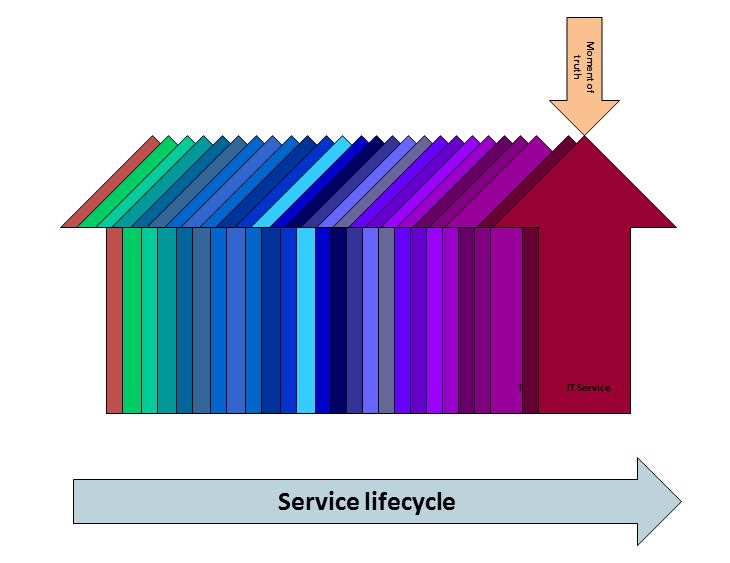
\includegraphics[width=0.48\textwidth]{images/svcLifecycle.png}}}}{Service lifecycle}\end{center}
\end{minipage}

 
\end{center}
 
Remember in Chapter 1 we talked of the user's \href{http://dm-academy.github.io/aitm/images/1_01-ITStack2.png}{value experience}, and also how services \href{http://dm-academy.github.io/aitm/#_the_it_service_lifecycle}{evolve over time in a lifecycle}?
 
There are two primary value experiences:
 \begin{itemize}

\item{} The value the user derives from the service (e.g. account lookups, or a flawless navigational experience)
 

\item{} The value the investor derives from monetizing the product, or comparable incentives (e.g. nonprofit missions)
 
\end{itemize}
 
Additionally, the product team derives career value. This becomes more of a factor later in the game. We will discuss this further in chapter 7 on organization, and Part IV on architecture lifecycles \& technical debt.
 
The product team receives feedback from both value experiences. The day to day interactions with the service (e.g. help desk and operations) are understood, and (typically on a more intermittent basis) the portfolio investor also feeds back the information to the product team (the boss's boss comes for a visit).
 
This is of course a simplified model, and in a large enterprise both the users and investors may have proxies (more on this to come).
 
\begin{center}
 
\noindent\begin{minipage}[c]{\linewidth}
\begin{center}
\imgexists{images/feedback1.png}{{\imgevalsize{images/feedback1.png}{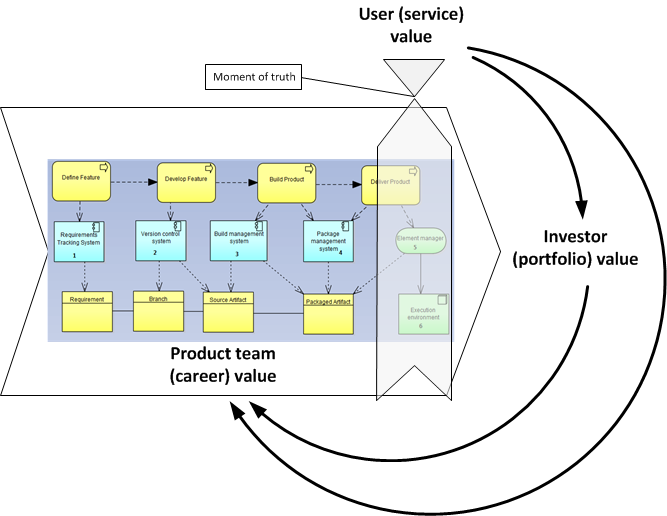
\includegraphics[width=0.48\textwidthkeepaspectratio=true]{images/feedback1.png}}}}{feedback1}\end{center}
\end{minipage}

 
\end{center}
 
The figure above is an architectural representation of the toolchain we started to develop in Section 1. The toolchain can be seen as part of a value chain that is delivering an IT service.
 
In this section, we will look at:
 \begin{itemize}

\item{} How you are accepting and executing on feedback signals
 

\item{} How the feedback relationship with your investors is evolving, in terms of your product direction
 

\item{} How the feedback relationship with your users is evolving, in terms of both operational criteria and product direction
 
\end{itemize}
 
We will discuss work management, product management, shared mental models, visualization, and systems monitoring.
 
The practices and approaches established at the team level are critical to the higher levels of scale discussed in Sections 3 and 4. In this section, we discuss small, cross-{}functional, outcome-{}oriented teams. We discuss collaboration and customer intimacy, and the need to limit work in process. And we discuss blameless cultures where people are safe to fail and learn.
 
If these learnings are not firmly established, the organization may struggle to scale; the need for cross-{}team coordination can (ironically) destroy the performance of individual teams, if not handled well. Scaling success starts with building a strong team level.
 
\textbf{Special section: Systems thinking} We talk of information \emph{systems}, but what are systems? There is a rich body of knowledge describing them, which we will touch on in this special section.
 
\textbf{Chapter 4: Product Management}
 
You (as the startup leader) are spending more time with investors and customers, and maintaining alignment around your original product vision is becoming more challenging as you are pulled in various directions. You need some means of keeping the momentum here. And the concept of "product management," you're finding, represents a rich set of ideas for managing your team's efforts at this stage of the game.
 
\textbf{Chapter 5: Work Management}
 
Even with a small team of 5 people (let alone 8 or 9), it's too easy for balls to get dropped as work moves between key contributors. You probably don't need a complex software-{}based process management tool yet, but you do need some way of managing work in process. And you start to understand that work takes many forms and exists as a concept at different scales.
 
\textbf{Chapter 6: Operations Management}
 
Since Chapter 3, your application developers have been running your systems and even answering the occasional phone call from customers. You're big enough that you need a bit more specialization. You've got dedicated support staff answering the phone calls and you are finding that, even if you rotate operational responsibilities across developers, it is still a distinct kind of "interrupt-{}driven" work that is not compatible with heads-{}down, focused software development. You've probably seen by now that complex systems are fragile and tend to fail; how you learn (or don't) from those failures is a critical question.
 \begin{DBKadmonition}{warning}{Important}
 
Part II, like the other parts, needs to be understood as a unified whole. In reality, startups struggle with the issues in all three chapters simultaneously.
 \end{DBKadmonition}
 
\label{systems-thinking}\hyperlabel{systems-thinking}
  
\section{Special section: Systems thinking and feedback}
\label{_special_section_systems_thinking_and_feedback}\hyperlabel{_special_section_systems_thinking_and_feedback}%
  \begin{quote}

"The harder you push, the harder the system pushes back."

\hspace*\fill--- Peter Senge
\emph{The Fifth Discipline} \end{quote}
 
\label{feedback}\hyperlabel{feedback}
 
\subsection{A brief introduction to feedback}
\label{_a_brief_introduction_to_feedback}\hyperlabel{_a_brief_introduction_to_feedback}%
  
While the term "information systems (IS)" was widely replaced by "information technology (IT)" in the 1990s, do not be fooled. Enterprise IT is a complex \href{https://en.wikipedia.org/wiki/Sociotechnical_system}{sociotechnical system}, that delivers the digital services to support a myriad of other complex sociotechnical systems.
 
Merriam-{}Webster \href{http://www.merriam-webster.com/dictionary/system}{defines a system} as "a regularly interacting or interdependent group of items forming a unified whole". These interactions and relationships quickly take center stage as you move from individual work to team efforts. Consider that while a 2 member team only has 1 relationship to worry about, a 10 member team has 45, and a 100 person team has 4,950!
 
As the Senge quote implies, brute force does not scale well within the context of a system. Systems tend to make their own rules. Within the bounds of the system, actions lead to outcomes, which in turn affect future actions. This \textbf{feedback} often becomes amplified and re-{}amplified through the systems' interactions with itself, until an overload occurs, such as the horrible screeching of a microphone too close to a speaker. In the business world, these feedback loops can manifest themselves in rigid platforms, brittle applications, or even a toxic work culture that sabotages success.
 
A thorough discussion of systems theory is beyond the scope of this book. However, many of the ideas that follow are informed by it. Obtaining a working knowledge of systems theory will not only enhance your understanding of this book, it can also be an essential tool for managing uncertainty in your future career, teams, and organizations. If you are interested in this topic, you might start with \emph{An Introduction to General Systems Thinking} by Gerald Weinberg \hyperlink{Weinberg2001}{[Weinberg2001]}.
 
Feedback is a loaded term. We hear terms like positive feedback and negative feedback, and associate it quickly with performance coaching and management discipline. That is not the sense of feedback in this book. The definition of feedback as used in this book is based on engineering. There is considerable related theory in general engineering and especially \href{https://en.wikipedia.org/wiki/Control_theory}{control theory} and the reader is encouraged to investigate some of these foundations if unfamiliar.
 
Here is the classic illustration of a feedback loop:
 \begin{wrapfigure}{r}{0.5\textwidth}[H]

\begin{center}
\imgexists{images/2_00-feedback.png}{{\imgevalsize{images/2_00-feedback.png}{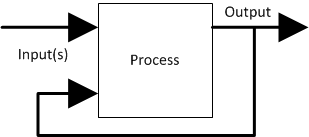
\includegraphics[width=0.48\textwidth]{images/2_00-feedback.png}}}}{feedback}
\end{center}
\caption{Classic feedback loop}
\end{wrapfigure}
 
For example, we can consider \textquotedblleft{}rabbit reproduction\textquotedblright{} as a process with a positive feedback loop:
 \begin{wrapfigure}{r}{0.5\textwidth}[H]

\begin{center}
\imgexists{images/2_00-rabbits.png}{{\imgevalsize{images/2_00-rabbits.png}{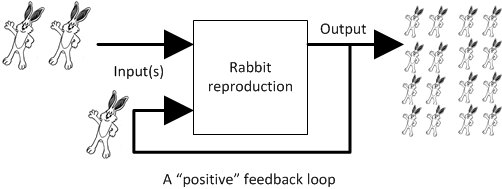
\includegraphics[width=0.48\textwidth]{images/2_00-rabbits.png}}}}{rabbits}
\end{center}
\caption{Rabbit reproduction}
\end{wrapfigure}
 
The more rabbits, the faster they reproduce, and the more rabbits.
 
This is a \textquotedblleft{}positive\textquotedblright{} feedback loop, although Mr. MacGregor the local gardener may not agree, given that they are eating all his cabbages!! This is why feedback experts (e.g. \hyperlink{Sterman2000}{[Sterman2000]}) prefer to call this \textquotedblleft{}reinforcing\textquotedblright{} feedback, because there is not necessarily anything \textquotedblleft{}positive\textquotedblright{} about it.
 
We can also consider feedback as the relationship between TWO processes:
 \begin{wrapfigure}{r}{0.5\textwidth}[H]

\begin{center}
\imgexists{images/2_00-processAB.png}{{\imgevalsize{images/2_00-processAB.png}{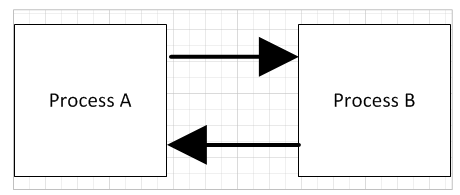
\includegraphics[width=0.48\textwidth]{images/2_00-processAB.png}}}}{feedback between 2 processes}
\end{center}
\caption{Feedback between two processes}
\end{wrapfigure}
 
In our rabbit example, what if Process B is fox reproduction, that is, the birth rate of foxes (who eat rabbits)?
 \begin{wrapfigure}{r}{0.5\textwidth}[H]

\begin{center}
\imgexists{images/2_00-rabbitfox.png}{{\imgevalsize{images/2_00-rabbitfox.png}{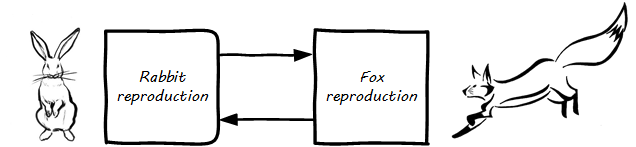
\includegraphics[width=0.48\textwidth]{images/2_00-rabbitfox.png}}}}{rabbits and foxes}
\end{center}
\caption{Balancing feedback}
\end{wrapfigure}
 
More rabbits equals more foxes (notice the \textquotedblleft{}+\textquotedblright{} symbol on the line), because there are more rabbits to eat! But what does this do to the rabbits? It means LESS rabbits. Which, ultimately, means less foxes\ldots{} and at some point, the populations balance. This is classic negative feedback. However, the local foxes don't see it as negative (nor do the local gardeners!)  That is why feedback experts prefer to call this \textquotedblleft{}balancing\textquotedblright{} feedback.
 
Wikipedia has good articles on \href{https://en.wikipedia.org/wiki/Causal_loop_diagram}{Causal Loop Diagramming} and \href{https://en.wikipedia.org/wiki/System_dynamics}{Systems Dynamics} (with cool dynamic visuals.) \hyperlink{Sterman2000}{[Sterman2000]} is the definitive text with applications.
  
\subsection{What does systems thinking have to do with IT?}
\label{_what_does_systems_thinking_have_to_do_with_it}\hyperlabel{_what_does_systems_thinking_have_to_do_with_it}%
  
In an engineering sense, positive feedback is often dangerous and a topic of concern. The classic example of bad positive feedback in engineering is the collapse of the Tacoma Narrows bridge, "Galloping Gertie."
 \begin{wrapfigure}{r}{0.5\textwidth}[H]

\begin{center}
\imgexists{images/2_00-bridge.jpg}{{\imgevalsize{images/2_00-bridge.jpg}{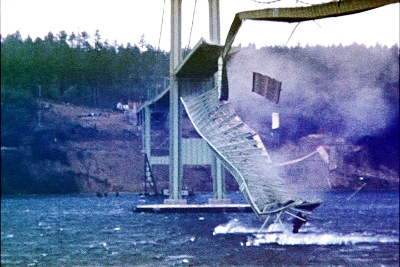
\includegraphics[width=0.48\textwidth]{images/2_00-bridge.jpg}}}}{collapsing bridge}
\end{center}
\caption[{"Galloping Gertie" }]{"Galloping Gertie" \footnotemark{}}
\end{wrapfigure}
 
As with bridges, at a technical level, reinforcing feedback can be a very bad thing in IT systems. In general, any process that is self-{}amplified without any balancing feedback will eventually consume all available resources, just like rabbits will eat all the food available to them. So, if you create a process (e.g. write and run a computer program) that recursively spawns itself, it will sooner or later crash the computer as it devours memory and CPU. See \href{http://osr507doc.sco.com/en/HANDBOOK/runaway_proc.html}{Runaway processes.}
 
Balancing feedback, on the other hand, is critical to make sure you are \textquotedblleft{}staying on track.\textquotedblright{} Engineers use concepts of \href{https://en.wikipedia.org/wiki/Control_theory}{control theory}, for example \href{https://en.wikipedia.org/wiki/Damping}{damping}, to keep bridges from falling down. Balancing feedback in a business and IT context takes a wide variety of forms:
 \begin{itemize}

\item{} The results of a product test in the marketplace, for example do the users prefer a drop down box or check boxes on a form?
 

\item{} The product owner clarifying for developers their user experience vision for the product, based on a demonstration of developer work in process
 

\item{} The end users calling to tell you the \textquotedblleft{}system is slow\textquotedblright{} (or down)
 

\item{} The product owner or portfolio sponsor calling to tell you they are not satisfied with the system's value
 
\end{itemize}
 
In short, we see these two basic kinds of feedback:
 \begin{itemize}

\item{} Positive/Reinforcing, \textquotedblleft{}do more of that\textquotedblright{}
 

\item{} Negative/Balancing, \textquotedblleft{}stop doing that,\textquotedblright{} \textquotedblleft{}fix that\textquotedblright{}
 
\end{itemize}
 \begin{DBKadmonition}{}{Note}
 
Still confused? Think about the last time you saw a "reply-{}all" email storm. The first accidental mass send generates feedback (emails saying "take me off this list"), which generate more emails ("stop emailing the list") and so on. This does not continue indefinitely; management intervention, common sense and fatigue eventually damp the storm down.
 \end{DBKadmonition}
 
One of the most important concepts related to feedback, one we will keep returning to, is that product value is based on feedback. We've discussed \hyperlink{lean-startup}{Lean Startup}, which represents a feedback loop intended to discover product value. Don Reinertsen, whose work we will discuss in this chapter, has written extensively on the importance of fast feedback to the product discovery process.
 
\subsubsection{Positive feedback: the special case investors want}
\label{_positive_feedback_the_special_case_investors_want}\hyperlabel{_positive_feedback_the_special_case_investors_want}%
  
At a business level, there is a special kind of positive feedback that defines the successful business:
 
\begin{center}
 
\noindent\begin{minipage}[c]{\linewidth}
\begin{center}
\imgexists{images/2_00-biz-positive.png}{{\imgevalsize{images/2_00-biz-positive.png}{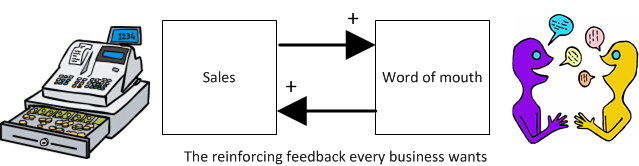
\includegraphics[width=0.48\textwidth]{images/2_00-biz-positive.png}}}}{positive business feedback}\end{center}
\end{minipage}

 
\end{center}
 
This is reinforcing feedback and positive for most people involved: investors, customers, employees.
 
At some point, if the cycle continues, it will run into balancing feedback:
 \begin{itemize}

\item{} Competition
 

\item{} Market saturation
 

\item{} Negative externalities (regulation, pollution, etc)
 
\end{itemize}
 
But those are the problems the business wants to have.
 
\label{open-loop}\hyperlabel{open-loop}
  
\subsubsection{Open versus closed loop systems}
\label{_open_versus_closed_loop_systems}\hyperlabel{_open_versus_closed_loop_systems}%
  
Finally, we should talk briefly about open loop versus closed loop systems.
 \begin{itemize}

\item{} Open loop systems have no regulation, no balancing feedback
 

\item{} Closed loop systems have some form of balancing feedback
 
\end{itemize}
 
In navigation terminology, the open-{}loop attempt to stick to a course without external information (e.g. navigating in the fog, without radar or communications) is known as " \href{https://en.wikipedia.org/wiki/Dead_reckoning}{dead reckoning}," in part because it can easily get you dead!
 
A good example of an open loop system is the children's game \textquotedblleft{}pin the tail on the donkey.\textquotedblright{} In \textquotedblleft{}pin the tail on the donkey,\textquotedblright{} a person has to execute a process (pinning a paper or cloth "tail" onto a poster of a donkey -{} no live donkeys are involved!) while blindfolded, based on their memory of their location (and perhaps after being deliberately disoriented by spinning in circles). Since they are blindfolded, they have to move across the room and pin the tail without the ongoing corrective feedback of their eyes. (Perhaps they are getting feedback from their friends, but perhaps their friends are not reliable\ldots{}.)
 \begin{wrapfigure}{r}{0.5\textwidth}[H]

\begin{center}
\imgexists{images/2_00-donkey.jpg}{{\imgevalsize{images/2_00-donkey.jpg}{\includegraphics[width=0.48\textwidth]{images/2_00-donkey.jpg}}}}{donkey game}
\end{center}
\caption[{Pin the tail on the donkey }]{Pin the tail on the donkey \footnotemark{}}
\end{wrapfigure}
 
Without the blindfold, it would be a closed loop system. The person would rise from their chair and, through the ongoing feedback of their eyes to their central nervous system, would move towards the donkey and pin the tail in the correct location.
 
This may seem obvious, but the history of IT management (some would say all management) over the past decades has been the struggle to overcome open-{}loop practices. Reliance on open-{}loop practices is arguably an indication of a dysfunctional command and control culture. A IT team that is designing and delivering without sufficient corrective feedback from its stakeholders is an ineffective, open-{}loop system. \hyperlink{Kennaley2010}{[Kennaley2010]} applies these principles to software development in much greater depth, and is recommended.
 \begin{DBKadmonition}{}{Note}
 
No system can ever be fully "open loop" indefinitely.  Sooner or later, you take off the blindfold, or wind up on the rocks. Mark Kennaley prefers the term "delayed feedback closed loop system" (personal correspondence, 9/2015).
 \end{DBKadmonition}
 
Engineers of complex systems use feedback techniques extensively. Complex systems do not work without them.
 
\label{OODA}\hyperlabel{OODA}
  
\subsubsection{OODA}
\label{_ooda}\hyperlabel{_ooda}%
  
After the Korean War, the US Air Force wished to clarify why its pilots had performed in a superior manner to the opposing pilots who were flying aircraft viewed as more capable. A colonel named John Boyd was tasked with researching the problem. His conclusions are based in the concept of feedback cycles, and how fast humans can execute them.  determined that humans go through a defined process in building their mental model of complex and dynamic situations. This has been formalized in the concept of the OODA loop. Standing for:
 \begin{itemize}

\item{} Observe
 

\item{} Orient
 

\item{} Decide
 

\item{} Act
 
\end{itemize}
 
Because the US fighters were lighter, more maneuverable, and had better visibility, their pilots were able to execute the OODA loop more quickly than their opponents, leading to victory. Boyd and others have extended this concept into various other domains including business strategy. The concept of the OODA feedback loop is frequently mentioned in presentations on Agile methods. Tightening the OODA loop accelerates the discovery of product value and is highly desirable.
 
\emph{Second draft ideas}
 
\begin{lstlisting}[firstnumber=1,backgroundcolor={},basicstyle=\ttfamily,]
==== Quality management
Deming and Juran.
\end{lstlisting}
 
\label{product-mgmt-chap}\hyperlabel{product-mgmt-chap}
    
\section{Chapter 4: Product Management}
\label{_chapter_4_product_management}\hyperlabel{_chapter_4_product_management}%
  

\begin{sidebar}

\textbf{Collaborative}

\begin{lstlisting}[firstnumber=1,backgroundcolor={},basicstyle=\ttfamily,]
Status 10/2016: This chapter is in "draft 1.5" - improved from original first draft completed in 2015.
\end{lstlisting}
\begin{itemize}

\item{} \href{https://github.com/dm-academy/aitm/blob/master/collaborator-instructions.adoc}{Collaborator instructions}
 

\item{} Raise an \href{https://github.com/dm-academy/aitm/issues}{issue} to comment
 

\item{} \href{https://github.com/dm-academy/aitm/tree/master/book}{Github source files}
 
\end{itemize}

\emph{Please remember that the intended audience of this one or two semester survey text is incoming students at a Masters' level in Information Technology, Information Systems, and Software Engineering programs. The most useful feedback comes from the perspective of, "what do you think today's students need to learn, given the last 20 years' developments with Agile, Lean IT, DevOps, web-{} and cloud-{}scale IT, digital transformation, and related themes?"}
\end{sidebar}
 
\subsection{Introduction}
\label{_introduction_4}\hyperlabel{_introduction_4}%
  

\begin{sidebar}

\textbf{Product Management?}

"Product management?" In a book on IT management? Those of you with industry experience, especially backgrounds in project-{}based enterprise software development, may be unfamiliar with the term. However, a focus on product development is one of the distinguishing features of Agile development, even if that development is taking place in a larger enterprise context.
\end{sidebar}
 
As you grow your company, you are bringing more people in. You become concerned that they need to share the same vision that inspired you to create this company. This is the goal of product management as a formalized practice.
 
Product strategy was largely tacit in Part I. As the founder, you used product management and discovery practices, and may well be familiar with the ideas here, but the assumption is that you did not explicitly \textbf{formalize} your approach to them. Now you need a more prescriptive and consistent approach to discovering, defining, designing, communicating, and executing a product vision across a diverse team.
 
In this chapter, we will define and discuss product management, and distinguish it from project and process management. We will cover how product teams are formed and what practices and attitudes you should establish quickly.
 
We will discuss a number of specific schools of thought and practices, including Gothelf's Lean UX, Scrum, and more specific techniques for product "discovery." Finally, we will discuss the concepts of design and design thinking.
 
\subsubsection{Chapter 4 outline}
\label{_chapter_4_outline}\hyperlabel{_chapter_4_outline}%
  \begin{itemize}

\item{} Why product management?
 \begin{itemize}

\item{} The product vision
 

\item{} Defining Product Management
 

\item{} Process, project, and product management
 

\item{} Productization as a strategy at Amazon
 
\end{itemize}
 

\item{} Organizing the product team
 \begin{itemize}

\item{} The concept of collaboration
 

\item{} Lean UX
 

\item{} Scrum
 

\item{} More on product team roles
 
\end{itemize}
 

\item{} Product discovery
 \begin{itemize}

\item{} Formalizing product discovery
 

\item{} Product discovery techniques
 

\item{} Discovery and design
 

\item{} Design
 
\end{itemize}
 

\item{} Assorted topics in Product Management
 
\end{itemize}
  
\subsubsection{Chapter 4 learning objectives}
\label{_chapter_4_learning_objectives}\hyperlabel{_chapter_4_learning_objectives}%
  \begin{itemize}

\item{} Define and distinguish product versus project and process management
 

\item{} Identify the key concerns of forming a collaborative product team
 

\item{} Describe current product-{}oriented practices, such as Lean UX and Scrum
 

\item{} Describe product design and discovery practices and concerns
 
\end{itemize}
 
\label{product-mgmt}\hyperlabel{product-mgmt}
   
\subsection{Why product management?}
\label{_why_product_management}\hyperlabel{_why_product_management}%
  
\subsubsection{The product vision}
\label{_the_product_vision}\hyperlabel{_the_product_vision}%
  \begin{DBKadmonition}{}{Note}
 
You should review the \hyperlink{digital-context}{digital context} material in Chapter 1.
 \end{DBKadmonition}
 \begin{wrapfigure}{r}{0.5\textwidth}[H]

\begin{center}
\imgexists{images/2_04-design.jpg}{{\imgevalsize{images/2_04-design.jpg}{\includegraphics[width=0.48\textwidth]{images/2_04-design.jpg}}}}{team meeting}
\end{center}
\caption[{Product design session }]{Product design session \footnotemark{}}
\end{wrapfigure}
 
Before work, before operations, there must be a vision of product. You already established a preliminary vision in Chapter 1, but now as your organization grows, you need to consider further how you will sustain that vision and establish an ongoing capability for realizing it. Like many other topics in this book, product management is a significant field in and of itself. Historically, product management has \textbf{not} been a major theme in enterprise IT management. Digital changes this.
 
IT systems started by serving narrow purposes, often \textquotedblleft{}back office\textquotedblright{} functions such as accounting or \href{https://en.wikipedia.org/wiki/Material_requirements_planning}{materials planning}. Mostly, such systems were managed as projects assembled on a temporary basis, resulting in the creation of a system to be \textquotedblleft{}thrown over the wall\textquotedblright{} to operations. Product management, on the other hand, is concerned with the entire lifecycle. The product manager (or owner, in Scrum terms) cares about the vision, its execution, the market reaction to the vision (even if an internal market), the health, care and feeding of the product, and the product's eventual sunset or replacement.
 
In the enterprise IT world, "third party" vendors (e.g. IBM) providing the back office systems had product management approaches, but these were \textbf{external} to the IT operations. Nor were IT-{}based product companies as numerous forty years ago as they are today; as noted in chapter 1, the digital component of modern products \hyperlink{digital-transformation}{continues to increase} to the point where it's often not clear whether a product is "IT" or not.
 
Reacting to market feedback and adapting product direction is an essential role of the product owner. In the older model, feedback was often unwelcome, as the project manager typically was committed to the \hyperlink{open-loop}{open-{}loop dead reckoning} of the project plan and changing scope or direction was seen as a failure, more often than not.
 
Now, it's accepted that systems evolve, perhaps in unexpected directions. Rapidly testing, failing fast, learning, and pivoting direction are all part of the lexicon, at least for market-{}facing IT-{}based products. And even back-{}office IT systems with better understood scope are being managed more as systems (or products) with lifecycles, as opposed to transient projects. (See the \hyperlink{amazon-productization}{Amazon discussion}, below.)
 
So, what is product management and what does it mean for your team?
 
\label{prod-mgmt-definition}\hyperlabel{prod-mgmt-definition}
  
\subsubsection{Defining Product Management}
\label{_defining_product_management}\hyperlabel{_defining_product_management}%
  
In order to define product management, we first need to define product. In Chapter 1, we established that products are goods, services, or some combination, with some feature that provides value for some consumer. BusinessDictionary.com \href{http://www.businessdictionary.com/definition/product.html}{defines it thus}:
 \begin{quote}

[A Product is] A good, idea, method, information, object or service created as a result of a process and serves a need or satisfies a want. It has a combination of tangible and intangible attributes (benefits, features, functions, uses) that a seller offers a buyer for purchase. For example a seller of a toothbrush not only offers the physical product but also the idea that the consumer will be improving the health of their teeth . . . A good or service [must] closely meet the requirements of a particular market and yield enough profit to justify its continued existence.

\hspace*\fill--- BusinessDictionary.com
\end{quote}
 
Product \emph{management}, according to the \href{http://www.businessdictionary.com/definition/product-management.html#ixzz3bHCVkoWj}{same source}, is
 \begin{quote}

The organizational structure within a business that manages the development, marketing and sale of a product or set of products throughout the product life cycle. It encompasses the broad set of activities required to get the product to market and to support it thereafter.

\hspace*\fill--- BusinessDictionary.com
\end{quote}
 
Product management in the general sense often reports to the Chief Marketing Officer (CMO). It represents the fundamental strategy of the firm, in terms of its value proposition and viability. The product needs to reflect the enterprise's strategy for creating and maintaining customers.
 
Product strategy for \textbf{internally-{}facing} products is usually \textbf{not} defined by the enterprise CMO. If it is a back-{}office product, then \textquotedblleft{}business within a business\textquotedblright{} thinking may be appropriate. (Even the payroll system run by IT for HR is a \textquotedblleft{}product,\textquotedblright{} in this view.) In such cases, there still is a need for someone to function as an "internal CMO" to the external "customers."
 \begin{DBKadmonition}{}{Note}
 
As a field, product management has a professional association, the \href{http://www.pdma.org}{Product Development and Marketing Association}, which publishes an extensive and continuously-{}refined handbook, and supports local chapters, training and certification, and other activities typical of a mature professional organization.
 \end{DBKadmonition}
 
With \hyperlink{digital-transformation}{digital transformation}, all kinds of industrial products have increasing amounts of \textquotedblleft{}IT\textquotedblright{} in them. This means that an understanding of IT, and ready access to any needed IT specialty skills, is increasingly important to the general field of product management. Product management includes research and development, which means that there is considerable uncertainty. This is of course also true of IT systems development.
 
Perhaps the most important aspect of product design is focusing on the user, and what she or he needs. The concept of \textbf{outcome} is key. This is easier said than done. The general problem area is considered Marketing, a core business school topic. Entire books have been written on the various tools and techniques for doing this, from  focus groups to ethnographic analysis.
 
\label{product-mgmt-v-marketing}\hyperlabel{product-mgmt-v-marketing}
 
However, Marty Cagan warns against confusing Product Management and Product Marketing. He defines the two as follows:
 
\emph{The product manager is responsible for defining\textemdash{}in detail\textemdash{}the product to be built, and validating that product with real customers and users. The product marketing person is responsible for telling the world about that product, including positioning, messaging and pricing, managing the product launch, providing tools for the sales channel to market and sell the product, and for leading key programs such as online marketing and influencer marketing programs.} \hyperlink{Cagan2008}{[Cagan2008]}, pp. 10-{}11.
 
We discuss some criticisms of overly marketing-{}driven approaches \hyperlink{jobs-to-be-done}{below}.
 
\label{process-project-product}\hyperlabel{process-project-product}
  
\subsubsection{Process, project, and product management}
\label{_process_project_and_product_management}\hyperlabel{_process_project_and_product_management}%
  
In the remainder of this book, we will continually encounter three major topics:
 \begin{itemize}

\item{} Product Management (Chapter 4)
 

\item{} Project Management (covered in Chapters 8 and 9)
 

\item{} Process Management (covered in Chapter 9)
 
\end{itemize}
 
They have an important commonality: \textbf{all of them are concepts for driving results across organizations.}
 
The Appendices have brief discussions of \hyperlink{project-mgmt}{project management} and \hyperlink{process-modeling}{process modeling}. Here are some of the key differences between process, project and product management in the context of digital services and systems:
 \begin{table}[htbp]
\begin{center}
\begingroup%
\setlength{\newtblsparewidth}{\linewidth-2\tabcolsep-2\tabcolsep-2\tabcolsep-2\tabcolsep}%
\setlength{\newtblstarfactor}{\newtblsparewidth / \real{100}}%

\begin{tabular}{lll}\hline
\multicolumn{1}{|p{33.3333\newtblstarfactor}|}{\raggedright\bfseries%
%
Process%
}&\multicolumn{1}{p{33.3333\newtblstarfactor}|}{\raggedright\bfseries%
%
Project%
}&\multicolumn{1}{p{33.3334\newtblstarfactor}|}{\raggedright\bfseries%
%
Product%
}\tabularnewline
\cline{1-1}\cline{2-2}\cline{3-3}\multicolumn{1}{|p{33.3333\newtblstarfactor}|}{\raggedright%
Task oriented
%
}&\multicolumn{1}{p{33.3333\newtblstarfactor}|}{\raggedright%
Deliverable oriented
%
}&\multicolumn{1}{p{33.3334\newtblstarfactor}|}{\raggedright%
Outcome oriented
%
}\tabularnewline
\cline{1-1}\cline{2-2}\cline{3-3}\multicolumn{1}{|p{33.3333\newtblstarfactor}|}{\raggedright%
Repeatable with a high degree of certainty
%
}&\multicolumn{1}{p{33.3333\newtblstarfactor}|}{\raggedright%
Executable with a medium degree of certainty
%
}&\multicolumn{1}{p{33.3334\newtblstarfactor}|}{\raggedright%
Significant component of research and development, less certain of outcome -{} empirical approaches required
%
}\tabularnewline
\cline{1-1}\cline{2-2}\cline{3-3}\multicolumn{1}{|p{33.3333\newtblstarfactor}|}{\raggedright%
Fixed time duration, relatively brief (weeks/months)
%
}&\multicolumn{1}{p{33.3333\newtblstarfactor}|}{\raggedright%
Limited time duration, often scoped to a year or less
%
}&\multicolumn{1}{p{33.3334\newtblstarfactor}|}{\raggedright%
No specific time duration; lasts as long as there is a need
%
}\tabularnewline
\cline{1-1}\cline{2-2}\cline{3-3}\multicolumn{1}{|p{33.3333\newtblstarfactor}|}{\raggedright%
Fixed in form, no changes usually tolerated
%
}&\multicolumn{1}{p{33.3333\newtblstarfactor}|}{\raggedright%
Difficult to change scope or direction, unless specifically set up to accommodate
%
}&\multicolumn{1}{p{33.3334\newtblstarfactor}|}{\raggedright%
Must accommodate market feedback and directional change
%
}\tabularnewline
\cline{1-1}\cline{2-2}\cline{3-3}\multicolumn{1}{|p{33.3333\newtblstarfactor}|}{\raggedright%
Used to deliver service value and operate system (the "Ops" in DevOps)
%
}&\multicolumn{1}{p{33.3333\newtblstarfactor}|}{\raggedright%
Often concerned with system design and construction, but typically not with operation (the "Dev" in DevOps)
%
}&\multicolumn{1}{p{33.3334\newtblstarfactor}|}{\raggedright%
Includes service concept and system design, construction, operations, and retirement (both "Dev" and "Ops")
%
}\tabularnewline
\cline{1-1}\cline{2-2}\cline{3-3}\multicolumn{1}{|p{33.3333\newtblstarfactor}|}{\raggedright%
Process owners concerned with adherence and continuous improvement of process. Otherwise can be narrow in perspective.
%
}&\multicolumn{1}{p{33.3333\newtblstarfactor}|}{\raggedright%
Project managers are trained in resource and timeline management, dependencies \& scheduling. They are not typically incented to adopt a long-{}term perspective.
%
}&\multicolumn{1}{p{33.3334\newtblstarfactor}|}{\raggedright%
Product managers need to have project management skills as well as understanding market dynamics, feedback, building long-{}term organizational capability
%
}\tabularnewline
\cline{1-1}\cline{2-2}\cline{3-3}\multicolumn{1}{|p{33.3333\newtblstarfactor}|}{\raggedright%
Resource availability and fungibility is assumed
%
}&\multicolumn{1}{p{33.3333\newtblstarfactor}|}{\raggedright%
Resources are specifically planned for but their commitment is temporary (team is "brought to the work")
%
}&\multicolumn{1}{p{33.3334\newtblstarfactor}|}{\raggedright%
Resources are assigned long-{}term to the product (work is "brought to the team")
%
}\tabularnewline
\hline
\end{tabular}\endgroup%

\end{center}

\caption{Process, project, and product management}
\end{table}
 
The above distinctions are deliberately exaggerated and there are of course exceptions (short projects, processes that take years). However, it is in the friction between these perspectives we see some of the major problems in modern IT management. For example, an activity, which may be a one-{}time task or a repeatable process, results in some work product (perhaps an artifact):
 \begin{wrapfigure}{r}{0.5\textwidth}[H]

\begin{center}
\imgexists{images/2_04-process.png}{{\imgevalsize{images/2_04-process.png}{\includegraphics[width=0.48\textwidth]{images/2_04-process.png}}}}{activities-{}work products}
\end{center}
\caption{Activities create work products}
\end{wrapfigure}
 
The consumer or stakeholder of that work product might be a Project Manager.
 
Project management includes concern for both the activities, AND the resources (people, assets, software) required to produce some deliverable:
 \begin{wrapfigure}{r}{0.5\textwidth}[H]

\begin{center}
\imgexists{images/2_04-project.png}{{\imgevalsize{images/2_04-project.png}{\includegraphics[width=0.48\textwidth]{images/2_04-project.png}}}}{projects-{}deliverables}
\end{center}
\caption{Projects create deliverables with resources and activities}
\end{wrapfigure}
 
The consumer of that deliverable might be a Product Manager.
 
Product management includes concern for projects and their deliverables, and their ultimate \textbf{outcomes} (either in the external market or internally):
 \begin{wrapfigure}{r}{0.5\textwidth}[H]

\begin{center}
\imgexists{images/2_04-product.png}{{\imgevalsize{images/2_04-product.png}{\includegraphics[width=0.48\textwidth]{images/2_04-product.png}}}}{Product-{}outcomes}
\end{center}
\caption{Product management may create outcomes with products}
\end{wrapfigure}
 
Notice that product management may directly access activities and resources. In fact, earlier-{}stage companies often do not formalize project management:
 \begin{wrapfigure}{r}{0.5\textwidth}[H]

\begin{center}
\imgexists{images/2_04-productNoProject.png}{{\imgevalsize{images/2_04-productNoProject.png}{\includegraphics[width=0.48\textwidth]{images/2_04-productNoProject.png}}}}{Product-{}outcomes2}
\end{center}
\caption{Product management sometimes does not use projects}
\end{wrapfigure}
 
In our scenario, you are now on a tight-{}knit, collaborative team. You should think in terms of developing and sustaining a product. However, projects still exist, and sometimes you may find yourself on a team that is funded and operated on that basis. You also will encounter the concept of "process" even on a single team; more on that in Chapter 5. We will go further into projects and process management in Part III.
 
\label{amazon-productization}\hyperlabel{amazon-productization}
  
\subsubsection{Productization as a strategy at Amazon}
\label{_productization_as_a_strategy_at_amazon}\hyperlabel{_productization_as_a_strategy_at_amazon}%
  
Amazon (the online bookseller) is an important influence in the modern trend towards product-{}centric IT management. First, the founder Jeff Bezos mandated that all software development should be \href{http://apievangelist.com/2012/01/12/the-secret-to-amazons-success-internal-apis/}{service-{}oriented}. That means that some form of standard API (Application Programming Interface) was required for all application to communicate with each other. (By some accounts, Bezos threatened to fire anyone who did not do this \hyperlink{Lane2012}{[Lane2012]}.) Second, all teams are to assume that the functionality being built might at some point be offered to external customers \hyperlink{Lane2012}{[Lane2012]}.
 \begin{wrapfigure}{r}{0.5\textwidth}[H]

\begin{center}
\imgexists{images/2_04-pizzas.jpg}{{\imgevalsize{images/2_04-pizzas.jpg}{\includegraphics[width=0.48\textwidth]{images/2_04-pizzas.jpg}}}}{pizzas}
\end{center}
\caption[{Can you feed your team with two pizzas? }]{Can you feed your team with two pizzas? \footnotemark{}}
\end{wrapfigure}
 
Second, a widely reported practice at Amazon.com is the \href{http://www.fastcompany.com/3037542/productivity-hack-of-the-week-the-two-pizza-approach-to-productive-teamwork}{limitation of product teams to between 5-{}7 people}, the number that can be fed by \textquotedblleft{}two pizzas\textquotedblright{} (depending on how hungry they are) \hyperlink{Gillet2014}{[Gillet2014]}. It has long been recognized in software and IT management that larger teams do not necessarily result in higher productivity. The best known statement of this is Fred Brooks' rule from The Mythical Man-{}Month, that \textquotedblleft{}adding people to a late project will make it later\textquotedblright{} \hyperlink{Brooks1975}{[Brooks1975]}.
 \begin{DBKadmonition}{}{Note}
 
Fred Brooks' \emph{The Mythical Man-{}Month}, derived in part from his experiences leading the IBM OS-{}360 project, is one of the timeless classics in software engineering and IT management writing. Serious IT professionals, whether or not they are actually programmers, should have it on their bookshelves.
 \end{DBKadmonition}
 
The reasons for "Brooks' Law" have been studied and analyzed (see e.g. \hyperlink{Madachy2008}{[Madachy2008]}, \hyperlink{Choi2016}{[Choi2016]}) but in general it is due to the increased communication overhead of expanded teams. Product design work (of which software development is one form) is creative and highly dependent on tacit knowledge, interpersonal interactions, organizational culture, and other \textquotedblleft{}soft\textquotedblright{} factors. Products, especially those with a significant IT component, can  be understood as socio-{}technical systems, often complex. This means that small changes to their components or interactions can have major effects on their overall behavior and value.
 
This in turn means that newcomers to a product development organization can have a profound impact on the product. Getting them \textquotedblleft{}up to speed\textquotedblright{} with the culture, mental models, and tacit assumptions of the existing team can be challenging and rarely is simple. And the bigger the team, the bigger the problem. The net result of these two practices at Amazon (and now \hyperlink{fowler-quote}{General Electric and many other companies}) is the creation of multiple nimble services that are decoupled from each other, constructed and supported by teams appropriately sized for optimal high-{}value interactions.
 
\label{the-product-team}\hyperlabel{the-product-team}
   
\subsection{Organizing the product team}
\label{_organizing_the_product_team}\hyperlabel{_organizing_the_product_team}%
  
You are a team now. Your founder and co-{}founder have found enough interest to sustain a larger organization.
 
How are you going to organize? How are you going to work? Events move quickly, and you don't have much time to think about these things. But getting things right at the team level is essential as your organization scales up. Bad habits (like accepting too much work in the system, or tolerating toxic individuals) will be more and more difficult to overcome as you grow.
 
\subsubsection{The concept of collaboration}
\label{_the_concept_of_collaboration}\hyperlabel{_the_concept_of_collaboration}%
  \begin{quote}

Individuals and interactions over processes and tools.  The most efficient and effective method of conveying information to and within a development team is face-{}to-{}face conversation.

\hspace*\fill--- Agile Manifesto
\end{quote}
 \begin{DBKadmonition}{warning}{Important}
 
We will discuss culture in more depth in future chapters. But this chapter  is the first discussion of "how are we with each other." Culture requires attention at the earliest stages, as it can be very difficult to change later.
 \end{DBKadmonition}
 
Team collaboration is one of the key values of Agile. The Agile Alliance states that
 
\emph{A "team" in the Agile sense is a small group of people, assigned to the same project or effort, nearly all of them on a full-{}time basis.}
 
Teams are multi-{}skilled, share accountability, and individuals on the team may play multiple roles. \hyperlink{Alliance2015}{[Alliance2015]}
 
\label{psych-safety}\hyperlabel{psych-safety}
 \begin{wrapfigure}{r}{0.5\textwidth}[H]

\begin{center}
\imgexists{images/2_04-psych-safety.jpg}{{\imgevalsize{images/2_04-psych-safety.jpg}{\includegraphics[width=0.48\textwidth]{images/2_04-psych-safety.jpg}}}}{happy faces}
\end{center}
\caption[{Psychological safety supports collaboration }]{Psychological safety supports collaboration \footnotemark{}}
\end{wrapfigure}
 
Face to face interactions, usually enabled by giving the team its own space, are seen as essential for collaboration. While there are various approaches to Agile, all concur that tight-{}knight, collaborative teams deliver the highest value outcomes.
 
However, collaboration does not happen just because people are fed pizzas and work in a room together. Google has established that the most significant predictor of team performance is a sense of psychological safety (see sidebar). Research by Anita Woolley and colleagues suggests that three factors drive team performance \hyperlink{Woolley2015}{[Woolley2015]}:
 \begin{itemize}

\item{} Equal contribution to team discussions (no dominant individuals)
 

\item{} Emotional awareness -{} being able to infer other team members' emotional states
 

\item{} Teams with a higher proportion of women tended to perform better (the researchers inferred this was due to women generally having higher emotional awareness)
 
\end{itemize}
 
Other research shows that diverse team and organizations are more innovative and deliver better results; such teams may tend to focus more on facts (as opposed to groupthink) \hyperlink{Rock2016}{[Rock2016]}. Certainly, a sense of psychological safety is critical to the success of diverse teams, who may come from different cultures and backgrounds that don't inherently trust each other.
 \begin{DBKadmonition}{warning}{Important}
 
The collective problem-{}solving talent of a diverse group of individuals who are given space to self-{}organize and solve problems creatively is immense, and very possibly the highest value resource known to the modern organization.
 \end{DBKadmonition}
 

\begin{sidebar}
\textbf{Google's Project Aristotle}


Around 2012, Google became interested in answering the question:

\textbf{\emph{What makes a Google team effective?}}

Based on 200+ interviews across 180+ teams, they determined that "Who is on a team matters less than how the team members interact, structure their work, and view their contributions."

They identified five "key dynamics":
\begin{enumerate}[label=\arabic*.]

\item{} Psychological safety: team members feel safe to take risks with each other
 

\item{} Dependability: team members can be counted on
 

\item{} Structure and clarity: roles, plans and goals are clear
 

\item{} Meaning of work: work is personally important
 

\item{} Impact of work: the work matters
 
\end{enumerate}

Of the 5, psychological safety was the most significant. Teams that cultivate this enable collaboration and creativity, which lead to product value and improved organizational performance. \hyperlink{Rozovsky2015}{[Rozovsky2015]}
\end{sidebar}
 
We turn to two current schools of thought with much to say about collaboration: Lean UX and Scrum.
  
\subsubsection{Lean UX}
\label{_lean_ux}\hyperlabel{_lean_ux}%
  \begin{quote}

Lean UX is the practice of bringing the true nature of a product to light faster, in a collaborative, cross-{}functional way that reduces the emphasis on thorough documentation while increasing the focus on building a shared understanding of the actual product experience being designed.

\hspace*\fill--- Jeff Gothelf
\emph{Lean UX} \end{quote}
 
Lean UX is a term coined by author and consultant Jeff Gothelf \hyperlink{Gothelf2013}{[Gothelf2013]}, which draws on three major influences:
 \begin{itemize}

\item{} Design thinking
 

\item{} Agile software development
 

\item{} Lean Startup
 
\end{itemize}
 
We briefly discussed \hyperlink{lean-startup}{Lean Startup} in Chapter 1, and the history and motivations for \hyperlink{Agile-history}{Agile software development} in Chapter 3. We'll look in more depth at product discovery techniques, and \hyperlink{design}{design and design thinking} in the next chapter section. However, Lean UX has much to say about forming the product team, suggesting (among others) the following principles for forming and sustaining teams:
 \begin{itemize}

\item{} Dedicated, cross-{}functional teams
 

\item{} Outcome (not deliverable/output) focus
 

\item{} Cultivating a sense of shared understanding
 

\item{} Avoiding toxic individuals (so-{}called "rockstars, gurus, and ninjas")
 

\item{} Permission to fail
 
\end{itemize}
 
(Other Lean UX principles such as small batch sizes and visualizing work will be discussed elsewhere; there is significant overlap between Lean UX and other schools of thought covered in this book.)
 
Lean UX is an influential work among digital firms and summarizes modern development practices well, especially for small, team-{}based organizations with minimal external dependencies. It is a broad and conceptual, principles-{}based framework open for interpretation in multiple ways. We continue with more "prescriptive" methods and techniques, such as Scrum.
 
\label{scrum}\hyperlabel{scrum}
  
\subsubsection{Scrum}
\label{_scrum}\hyperlabel{_scrum}%
  \begin{quote}

Scrum is a lightweight framework designed to help small, close-{}knit teams of people develop complex products.

\hspace*\fill--- Chris Sims/Hillary L. Johnson
\emph{Scrum: A Breathtakingly Brief and Agile Introduction} \end{quote}
 \begin{quote}

There Are No Tasks; There Are Only Stories.

\hspace*\fill--- Jeff Sutherland
\emph{Scrum: The Art of Doing Twice the Work in Half the Time} \end{quote}
 
One of the first prescriptive Agile methodologies you are likely to encounter as a practitioner is Scrum. There are many books, classes, and websites where you can learn more about this framework; \hyperlink{Sims2012}{[Sims2012]} is a good brief introduction, and \hyperlink{Rubin2012}{[Rubin2012]} is well suited for more in-{}depth study.
 \begin{DBKadmonition}{}{Note}
 
"Prescriptive" means detailed and precise. A doctor's prescription is specific as to what medicine to take, how much, and when. A prescriptive method is similarly specific. "Agile software development" is not prescriptive; as currently published by the Agile Alliance, it is a collection of principles and ideas you may or may not use.  By comparison, Scrum is prescriptive; it states roles and activities specifically and trainers and practitioners in general seek to follow the method completely and accurately.
 \end{DBKadmonition}
 
Scrum is appropriate to this chapter, as it is product-{}focused. It calls for the roles of:
 \begin{itemize}

\item{} Product owner
 

\item{} Scrum master
 

\item{} Team member
 
\end{itemize}
 
and avoids further elaboration of roles.
 
The Scrum product owner is responsible for holding the product vision and seeing that the team executes the highest value work. To do this, the potential features for the product are maintained in a "backlog" that can be re-{}prioritized as necessary (rather than a large, fixed-{}scope project). The product owner also defines acceptance criteria for the backlog items. The Scrum Master, on the other hand, acts as a team coach, "guiding the team to ever-{}higher levels of cohesiveness, self-{}organization, and performance." \hyperlink{Sims2012}{[Sims2012]}. To quote Roman Pichler:
 
\emph{The product owner and ScrumMaster roles complement each other: The product owner is primarily responsible for the "what"\textemdash{}creating the right product. The ScrumMaster is primarily responsible for the "how"\textemdash{}using Scrum the right way} \hyperlink{Pichler2010}{[Pichler2010]}, p. 9.
 
Scrum uses specific practices and artifacts such as sprints, standups, reviews, the above-{}mentioned concept of backlog, burndown charts, and so forth. We will discuss some of these further in Chapter 5 (Work Management) and Chapter 9 (Execution Management) along with Kanban, another popular approach for executing work.
 
In Scrum, there are three roles:
 \begin{itemize}

\item{} The product owner sets overall direction.
 

\item{} The Scrum Master coaches and advocates for the team
 

\item{} The development team is defined as those who are committed to the development work
 
\end{itemize}
 
There are seven activities:
 \begin{itemize}

\item{} The \textquotedblleft{}sprint\textquotedblright{} is a defined time period, typically two to four weeks, in which the development team executes on an agreed scope
 

\item{} Backlog grooming is when the product backlog is examined and refined into increments that can be moved into the sprint backlog
 

\item{} Sprint Planning is where the scope is agreed
 

\item{} The Daily Scrum is traditionally held standing up, to maintain focus and ensure brevity
 

\item{} Sprint Execution is the development activity within the sprint
 

\item{} Sprint Review is the \textquotedblleft{}public end of the sprint\textquotedblright{} when the stakeholders are invited to view the completed work
 

\item{} The Sprint Retrospective is held to identify lessons learned from the sprint and how to apply them in future work.
 
\end{itemize}
 
There are a number of artifacts:
 \begin{itemize}

\item{} The product backlog is the overall \textquotedblleft{}to-{}do\textquotedblright{} list for the product.
 

\item{} The sprint backlog is the to-{}do list for the current sprint
 

\item{} Potentially shippable product increment is an important concept used to decouple the team's development activity from downstream business planning. A PSI is a cohesive unit of functionality that \textbf{could} be delivered to the customer, but doing so is the decision of the product owner.
 
\end{itemize}
 
Scrum is well grounded in various theories (process control, human factors), although Scrum team members do not need to understand theory to succeed with it. Like Lean UX, Scrum emphasizes high-{}bandwidth collaboration, dedicated multi-{}skilled teams, a product focus, and so forth.
 
The concept of having an empowered product owner readily available to the team is attractive, especially for digital professionals who may have worked on teams where direction was unclear. Roman Pichler identifies a number of common mistakes, however, that diminish the value of this approach \hyperlink{Pichler2010}{[Pichler2010]}, pp. 17-{}20:
 \begin{itemize}

\item{} Product owner lacks authority
 

\item{} Product owner is overworked
 

\item{} Product ownership is split across individuals
 

\item{} Product owner is "distant" -{} not co-{}located or readily available to team
 
\end{itemize}
 

\begin{sidebar}

\textbf{Sidebar: Scrum and shu-{}ha-{}ri}

In the Japanese martial art of aikido, there is the concept of shu-{}ha-{}ri, a form of learning progression.
\begin{itemize}

\item{} Shu: The student follows the rules of a given method precisely, without addition or alteration
 

\item{} Ha: The student learns theory and principle of the technique
 

\item{} Ri: The student creates own approaches and adapts technique to circumstance
 
\end{itemize}

Scrum at its most prescriptive can be seen as a shu-{}level practice; it gives detailed guidance that has been shown to work.

(See \hyperlink{Fowler2006}{[Fowler2006]} and \hyperlink{Cockburn2007}{[Cockburn2007]}, pp. 17-{}18.)
\end{sidebar}
  
\subsubsection{More on product team roles}
\label{_more_on_product_team_roles}\hyperlabel{_more_on_product_team_roles}%
  \begin{quote}

Boundaries are provided by the product owner and often come in the form of constraints, such as * I need it by June. * We need to reduce the per-{}unit cost by half. * It needs to run at twice the speed.
* It can use only half the memory of the current version.

\hspace*\fill--- Mike Cohn
\emph{Succeeding with Agile Software Development Using Scrum} \end{quote}
 
\label{vuf}\hyperlabel{vuf}
 
Marty Cagan suggests that the product team has three primary concerns, requiring three critical roles \hyperlink{Cagan2008}{[Cagan2008]}, (ch.12):
 \begin{itemize}

\item{} Value: Product Owner/Manager
 

\item{} Feasibility: Engineering
 

\item{} Usability: User Experience Design
 
\end{itemize}
 
Jeff Patton represents these concepts as a Venn diagram:
 \begin{wrapfigure}{r}{0.5\textwidth}[H]

\begin{center}
\imgexists{images/2_04-VUF.png}{{\imgevalsize{images/2_04-VUF.png}{\includegraphics[width=0.48\textwidth]{images/2_04-VUF.png}}}}{venn diagram}
\end{center}
\caption[{The 3 views of the product team }]{The 3 views of the product team \footnotemark{}}
\end{wrapfigure}
 
\label{prod-mgr-v-own}\hyperlabel{prod-mgr-v-own}
 
Finally, a word on the product manager. \hyperlink{scrum}{Scrum} is prescriptive around the product \textbf{owner} role, but does not identify a role for product \textbf{manager}. This can lead to two people performing product management: a marketing-{}aligned "manager" responsible for high-{}level requirements, with the Scrum "product owner" attempting to translate them for the team. Marty Cagan warns against this approach, recommending instead that the product manager and owner be the same person, separate from marketing \hyperlink{Cagan2008}{[Cagan2008]}, pp. 7-{}8.
 
In the next chapter, we will consider the challenge of product discovery\hspace{0.167em}\textemdash{}\hspace{0.167em}at a product level, what practices do we follow to generate the creative insights that will result in customer value?
 
\begin{lstlisting}[firstnumber=1,backgroundcolor={},basicstyle=\ttfamily,]
more on self-organization
\end{lstlisting}
 
\label{prod-discovery}\hyperlabel{prod-discovery}
   
\subsection{Product discovery}
\label{_product_discovery}\hyperlabel{_product_discovery}%
  \begin{quote}

 What is a Product Manager? A Product Manager is the one person in the whole organization who owns the product Requirements effort. Requirements focuses on the WHAT, which means it isn't Development, which focuses on the HOW. And Marketing traditionally talks about the WHAT, but cannot necessarily decide what the WHAT should be. At least not at any useful level of detail. \hyperlink{Murphy2007}{[Murphy2007]}

\hspace*\fill--- Jacques Murphy
\emph{Pragmatic Marketing} \end{quote}
 
Now that we have discussed the overall concept of product management and why it is important, and how product teams are formed, we can turn more specifically to the topic of product discovery and design. We have previously discussed the overall \hyperlink{digital-context}{digital business context}, as a startup founder might think of the problem. But the process of discovery continues as the product idea is refined, new business problems are identified, and solutions (such as specific feature ideas) are designed and tested for outcomes.
 \begin{DBKadmonition}{}{Note}
 
In this book, we favor the idea that products are "discovered" as much or more than they are "designed." But you will see both terms used throughout this chapter. See the parable \hyperlink{flower-and-cog}{the Flower and the Cog} for an illustration of the difference.
 \end{DBKadmonition}
 
The presence of a section entitled "product discovery" in this book is a  departure from other IT management textbooks. "Traditional" models of IT delivery focus on projects and deliverables, concepts we touched on in the  \hyperlink{process-project-product}{last chapter section} but that we will not explore in depth until later in the book. However, the idea of "product discovery" \textbf{within} the large company is receiving more and more attention. Even large companies \hyperlink{fowler-quote}{benefit} when products are developed with tight-{}knit teams using fast feedback.
 \begin{DBKadmonition}{}{Note}
 
The term "intrapreneurship," credited to Gifford Pinchot, means "entrepreneurship inside a large company."
 \end{DBKadmonition}
 
For our discussion here, the challenge with the ideas of projects and deliverables is that they represent approaches that are more \hyperlink{open-loop}{open loop}, or at least delayed in \hyperlink{feedback}{feedback}. Design processes do not perform well when feedback is delayed. \hyperlink{system-intent}{System intent}, captured as a user story or requirement, is only an hypothesis until tested via implementation and user confirmation.
 
\label{prod-discovery-techniques}\hyperlabel{prod-discovery-techniques}
 
\subsubsection{Formalizing product discovery}
\label{_formalizing_product_discovery}\hyperlabel{_formalizing_product_discovery}%
  \begin{quote}

It is humbling to see how bad experts are at estimating the value of features (us included).

\hspace*\fill--- Ronnie Kohavi
\emph{Online Experimentation at Microsoft} \end{quote}
 
In Chapter 3, we needed to consider the means for describing  \hyperlink{system-intent}{system intent}. Even as a bare-{}bones startup, some formalization of this starts to emerge, at the very least in the form of test-{}driven development:
 \begin{wrapfigure}{r}{0.5\textwidth}[H]

\begin{center}
\imgexists{images/2_04-simplePipeline.png}{{\imgevalsize{images/2_04-simplePipeline.png}{\includegraphics[width=0.48\textwidth]{images/2_04-simplePipeline.png}}}}{pipeline}
\end{center}
\caption{Product discovery tacit}
\end{wrapfigure}
 
But, the assumption in our emergence model is that more formalized product management emerges with the formation of a team. As a team, we now need to expand "upstream" of the core delivery pipeline, so that we can collaborate and discover more effectively. Notice the grey box in the following:
 \begin{wrapfigure}{r}{0.5\textwidth}[H]

\begin{center}
\imgexists{images/2_04-PipelinewProdDisc.png}{{\imgevalsize{images/2_04-PipelinewProdDisc.png}{\includegraphics[width=0.48\textwidth]{images/2_04-PipelinewProdDisc.png}}}}{pipeline w product discovery}
\end{center}
\caption{Product discovery explicit}
\end{wrapfigure}
 
\label{HIPPO}\hyperlabel{HIPPO}
 
The most important foundation for your newly formalized product discovery capability is that it must be \textbf{empirical and hypothesis-{}driven}. Too often, product strategy is based on the HIPPO: The Highest Paid Person's Opinion.
 \begin{wrapfigure}{r}{0.5\textwidth}[H]

\begin{center}
\imgexists{images/2_04-hippo.jpg}{{\imgevalsize{images/2_04-hippo.jpg}{\includegraphics[width=0.48\textwidth]{images/2_04-hippo.jpg}}}}{hippopotamus}
\end{center}
\caption[{Beware of HIPPO-{}based product discovery }]{Beware of HIPPO-{}based product discovery \footnotemark{}}
\end{wrapfigure}
 
The problem with relying on "gut feel" or personal opinions is that people\hspace{0.167em}\textemdash{}\hspace{0.167em}regardless of experience or seniority\hspace{0.167em}\textemdash{}\hspace{0.167em}perform poorly in assessing the likely outcome of their product ideas. Some well known research on this topic was conducted by Microsoft's Ronny Kohavi. In this research, Kohavi and team determined that "only about 1/3 of ideas improve the metrics they were designed to improve." \hyperlink{Kohavi2009}{[Kohavi2009]} As background, the same report cites that:
 \begin{itemize}

\item{} "Netflix considers 90\% of what they try to be wrong"
 

\item{} "75 percent of important business decisions and business improvement ideas either have no impact on performance or actually hurt performance" according to Qualpro (a consultancy specializing in controlled experiments)
 
\end{itemize}
 

\begin{sidebar}
\textbf{Amazon Shopping Cart Recommendations}


A well known story of the power of experimentation is told by Greg Linden, who was a product developer for early versions of the Amazon shopping cart. Linden had an idea of making recommendations to people based on what was already in their shopping cart. (While this is common across e-{}commerce sites now, at one point it was a new idea.) While grocery stores "recommnend" impulse purchases (candy, gum) in the checkout lane, an ecommerce provider can recommend anything in the store, so the idea is even more powerful. Linden developed a prototype, and while it got some favorable reactions, one senior vice president was against it\hspace{0.167em}\textemdash{}\hspace{0.167em}his view was that it might distract people and lead them to abandon the cart.

As Linden says, "I was forbidden to work on this any further." But he went ahead and prepared the feature anyways. The SVP was furious, but Amazon already had a data-{}driven culture and even senior executives couldn't block tests. The feature was then pushed out to a small set of Amazon customers.  In this way, they could compare the behavior of customers who did receive shopping cart recommendations to those who didn't (otherwise known as a controlled experiment.) The results were dramatic -{} the feature outperformed the control of not having it by such a large margin that, as Linden says, "not having it live was costing Amazon a notable chunk of change."

It's unknown what happened to the SVP. Challenging senior executives can be bad for your career, but if you find yourself in a place run by HiPPOs who don't want to experiment, you might want to consider how long that organization will be in business.
\hyperlink{Linden2006}{[Linden2006]}
\end{sidebar}
 
It is therefore critical to establish a strong practice of data-{}driven experimentation when forming a product team, and avoid any cultural acceptance of "gut feel" or deferring to HIPPOs. This can be a difficult transition for the company founder, who has until now served as the \emph{de facto} product manager.
 
\label{DIBB}\hyperlabel{DIBB}
 
A useful framework, similar to \hyperlink{lean-startup}{Lean Startup} is proposed by Spotify, in the "DIBB" model:
 \begin{itemize}

\item{} Data
 

\item{} Insight
 

\item{} Belief
 

\item{} Bet
 
\end{itemize}
 
Data leads to insight, which leads to a hypothesis that can be tested (i.e., "bet" on -{} testing hypotheses is not free). We discuss issues of prioritization further in Chapter 5, in the section on \hyperlink{cost-of-delay}{Cost of Delay}.
 
\label{beneficial-variability}\hyperlabel{beneficial-variability}
 
Don Reinertsen (who we will read more about in the next chapter) emphasizes that such experimentation is inherently \emph{variable}. We can't develop experiments with any sort of expectation that they will always succeed. We might run 50 experiments, and only have 2 succeed. But if the cost of each experiment is \$10,000, and the two that succeeded earned us \$1 million each, we gained:
 
\begin{lstlisting}[firstnumber=1,backgroundcolor={},basicstyle=\ttfamily,]
$ 2,000,000
$ - 480,000
-----------
$ 1,520,000
\end{lstlisting}
 
Not a bad return on investment! (See \hyperlink{Reinertsen2009}{[Reinertsen2009]}, Chapter 4, for a detailed, mathematical discussion, based on options and information theory.) Roman Pichler, in \emph{Agile Product Management with Scrum}, describes "old-{}school" versus "new-{}school" product management this way:
 \begin{table}[htbp]
\begin{center}
\begingroup%
\setlength{\newtblsparewidth}{\linewidth-2\tabcolsep-2\tabcolsep-2\tabcolsep}%
\setlength{\newtblstarfactor}{\newtblsparewidth / \real{100}}%

\begin{tabular}{ll}\hline
\multicolumn{1}{|p{50\newtblstarfactor}|}{\raggedright\bfseries%
%
Old school%
}&\multicolumn{1}{p{50\newtblstarfactor}|}{\raggedright\bfseries%
%
New school%
}\tabularnewline
\cline{1-1}\cline{2-2}\multicolumn{1}{|p{50\newtblstarfactor}|}{\raggedright%
Shared responsibility
%
}&\multicolumn{1}{p{50\newtblstarfactor}|}{\raggedright%
Single product owner
%
}\tabularnewline
\cline{1-1}\cline{2-2}\multicolumn{1}{|p{50\newtblstarfactor}|}{\raggedright%
Detached project manager
%
}&\multicolumn{1}{p{50\newtblstarfactor}|}{\raggedright%
PM belongs to Scrum team
%
}\tabularnewline
\cline{1-1}\cline{2-2}\multicolumn{1}{|p{50\newtblstarfactor}|}{\raggedright%
Extensive up-{}front research
%
}&\multicolumn{1}{p{50\newtblstarfactor}|}{\raggedright%
Minimal up-{}front work to define rough vision
%
}\tabularnewline
\cline{1-1}\cline{2-2}\multicolumn{1}{|p{50\newtblstarfactor}|}{\raggedright%
Requirements frozen early
%
}&\multicolumn{1}{p{50\newtblstarfactor}|}{\raggedright%
Dynamic backlog
%
}\tabularnewline
\cline{1-1}\cline{2-2}\multicolumn{1}{|p{50\newtblstarfactor}|}{\raggedright%
Late feedback due to lengthy release cycle
%
}&\multicolumn{1}{p{50\newtblstarfactor}|}{\raggedright%
Early \& frequent releases drive fast feedback, resulting in customer value
%
}\tabularnewline
\hline
\end{tabular}\endgroup%

\end{center}

\caption[{Old school versus new school product management }]{Old school versus new school product management \footnotemark{}}
\end{table}
\addtocounter{footnote}{-1}\stepcounter{footnote}
\footnotetext{
summarized from \hyperlink{Pichler2010}{[Pichler2010]}, p. xxi
}  
\subsubsection{Product discovery techniques}
\label{_product_discovery_techniques}\hyperlabel{_product_discovery_techniques}%
  
There are a wide variety of techniques and even "schools" of product discovery and design; we will consider a few representatives in this chapter section. Of course, when you first started your journey in Chapter 1, you might also have used some of these techniques. But now that you are a team, you are formalizing and relying on these techniques. These techniques are not mutually exclusive; they may be complementary. But at the more detailed, digital product level, how do we develop hypotheses for testing, in terms of our products/services? We briefly mentioned User Story Mapping in our discussion of \hyperlink{system-intent}{system intent.} In product discovery terms, User Story Mapping is a form of persona analysis. But that is only one of many techniques. Roman Pichler mentions "Vision Box and Trade Journal Review" and the "Kano Model" (\hyperlink{Pichler2010}{[Pichler2010]}, p. 39). Here, let's discuss:
 \begin{itemize}

\item{} "Jobs to be done" analysis
 

\item{} Impact mapping
 

\item{} Business analysis \& architecture
 
\end{itemize}
 
\label{jobs-to-be-done}\hyperlabel{jobs-to-be-done}
 
\paragraph{Job to Be Done}
\label{_job_to_be_done}\hyperlabel{_job_to_be_done}%
  \begin{quote}

Customers don't want a quarter-{}inch drill. They want a quarter-{}inch hole.

\hspace*\fill--- Theodore Levitt
\end{quote}
 \begin{quote}

If I'd asked the customer what they wanted, they would have said "faster horses."

\hspace*\fill--- Henry Ford
\emph{(apocryphal)} \end{quote}
 
The "Jobs to be Done" framework was created by noted Harvard professor Clayton Christensen, in part as a reaction against conventional \hyperlink{product-mgmt-v-marketing}{marketing} techniques that
 
\emph{"frame customers by attributes\textemdash{}using age ranges, race, marital status, and other categories that ultimately create products and entire categories too focused on what companies want to sell, rather than on what customers actually need."} \hyperlink{Christensen2015}{[Christensen2015]}
 
"Some products are better defined by the job they do than the customers they serve," in other words. \hyperlink{Traynor2016}{[Traynor2016]} This is in contrast to many kinds of business and requirements analysis that focus on identifying different user personas (e.g. 45-{}55 married Black woman with children in the house). Jobs to be Done advocates argue that "The job, not the customer, is the fundamental unit of analysis" and that customer "hire" products to do a certain job. \hyperlink{Christensen2006}{[Christensen2006]}
 
To apply the Job to Be done approach, Des Traynor suggests filling in the blanks in the following \hyperlink{Traynor2016}{[Traynor2016]} :
 
\textbf{Why do people hire your product?}
 
People hire your product to do the job of -{}-{}-{}-{}-{}-{}-{}-{}  every -{}-{}-{}-{}-{}-{}-{}-{}-{}-{} when -{}-{}-{}-{}-{}-{}-{}-{}-{}-{}. The other applicants for this job are -{}-{}-{}-{}-{}-{}-{}-{}, -{}-{}-{}-{}-{}-{}-{}-{}, and -{}-{}-{}-{}-{}-{}-{}-{}, but your product will always get the job because of -{}-{}-{}-{}-{}-{}-{}-{}.
 
Understanding the alternatives people have is key. It's possible that the job can be fulfilled in multiple different ways. For example, people may want certain software run. This job can be undertaken through owning a computer (e.g. having a data center). It can also be managed by hiring someone else's computer (e.g. using a Cloud provider). If one is not attentive and creative in thinking about the diverse ways jobs can be done, one is at risk for disruption.
 
\label{impact-mapping}\hyperlabel{impact-mapping}
  
\paragraph{Impact mapping}
\label{_impact_mapping}\hyperlabel{_impact_mapping}%
  
Understanding the relationship of a given feature or component to business objectives is critical. Too often, technologists (e.g software professionals) are accused of wanting "technology for technology's sake."
 
Showing the "line of sight" from technology to a business objective is therefore critical. Ideally, this starts by identifying the business objective. Gojko Adzic's \emph{Impact Mapping: Making a big impact with software products and projects} \hyperlink{Adzic2012}{[Adzic2012]} describes a technique for doing so:
 
\emph{An impact map is a visualisation of scope and underlying assumptions, created collaboratively by senior technical and business people.}
 
Starting with some general goal or hypothesis (e.g. generated through Lean Startup thinking), one builds a "map" of how the goal can be achieved, or hypothesis can be measured. A simple graphical approach can be used:
 \begin{wrapfigure}{r}{0.5\textwidth}[H]

\begin{center}
\imgexists{images/2_04-impactMap.png}{{\imgevalsize{images/2_04-impactMap.png}{\includegraphics[width=0.48\textwidth]{images/2_04-impactMap.png}}}}{impact map}
\end{center}
\caption{Impact map}
\end{wrapfigure}
 \begin{DBKadmonition}{}{Note}
 
Impact mapping is similar to mind mapping, and some drawing tools such as Microsoft Visio come with "Mind Mapping" templates.
 \end{DBKadmonition}
 
The most important part of the impact map is to answer the question "Why are we doing this?" The impact map is intended to help keep the team focused on the most important objectives, and avoid less valuable activities and investments.
 
For example, in the above diagram, we see that a bank may have an overall business goal of customer retention. (It is much more expensive to gain a new customer, than to retain an existing one, and retention is a metric carefully measured and tracked at the highest levels of the business.)
 
Through focus groups and surveys, the bank may determine that staying current with online services is important to retaining customers. Some of these services are accessed by home PCs, but increasingly customers want access via mobile devices.
 
These business drivers lead to the decision to invest in online banking applications for both the Apple and Android mobile platforms. This decision in turn will lead to further discovery, analysis, and design of the mobile applications.
 
\label{biz-analysis-ch1}\hyperlabel{biz-analysis-ch1}
  
\paragraph{The Business Analysis Body of Knowledge}
\label{_the_business_analysis_body_of_knowledge}\hyperlabel{_the_business_analysis_body_of_knowledge}%
  
One well-{}established method for product discovery is that of business analysis, formalized in the \emph{Business Analysis Body of Knowledge} (BABOK), from the International Institute of Business Analysis \hyperlink{IIBA2015}{[IIBA2015]}
 
The Business Analysis Body of Knowledge (BABOK) defines business analysis as (p. 442):
 
\emph{The practice of enabling change in the context of an enterprise
by defining needs and recommending solutions that deliver value to
stakeholders}.
 
BABOK is centrally concerned with the concept of requirements, and classifies them thus:
 \begin{itemize}

\item{} Business requirements
 

\item{} Stakeholder requirements
 

\item{} Solution requirements
 \begin{itemize}

\item{} Functional requirements
 

\item{} Non-{}functional requirements
 
\end{itemize}
 

\item{} Transition requirements
 
\end{itemize}
 
BABOK also provides a framework for understanding and managing the work of business analysts; in general it assumes that a BA capability will be established and that maturing such a capability is a desirable thing. This may run counter to the Scrum ideal of cross-{}functional, multi-{}skilled teams. Also as noted \hyperlink{system-intent}{above}, the term "requirements" has fallen out of favor with some Agile thought leaders.
 
\label{design}\hyperlabel{design}
    
\subsection{Product design}
\label{_product_design}\hyperlabel{_product_design}%
  
\begin{center}
 
\noindent\begin{minipage}[c]{\linewidth}
\begin{center}
\imgexists{images/2_04-design2.jpg}{{\imgevalsize{images/2_04-design2.jpg}{\includegraphics[width=0.48\textwidth]{images/2_04-design2.jpg}}}}{Design sign}\end{center}
\end{minipage}

 
\end{center}
 
\footnote{
\emph{Image credit \href{https://www.flickr.com/photos/djs1021/101948321/}{https://www.flickr.com/\-photos/\-djs1021/\-101948321/\-}, downloaded 2016-{}09-{}19, commercial use permitted}
}
 \begin{quote}

Everyone designs who devises courses of action aimed at changing existing situations into preferred ones \hyperlink{Simon1988}{[Simon1988]}.

\hspace*\fill--- Herbert Simon
\end{quote}
 \begin{quote}

The art of making useful things beautiful and beautiful things useful.

\hspace*\fill--- unknown
\end{quote}
 
Once we have discovered at least a direction for the product's value proposition, and have started to understand and prioritize the functions it must perform, we begin the activity of \emph{design}. Design, like most other topics in this survey text, is a broad and complex area with varying definitions and schools of thought. The Herbert Simon quote at the beginning of this Part Is frequently cited.
 
Design is an ongoing theme throughout the humanities, encountered in architecture (the non-{}IT variety), art, graphics, fashion, and commerce. It can be narrowly focused, such as the question of what color scheme to use on an app or web page. Or it can be much more expansive, as suggested by the field of design thinking. We'll start from the expansive vision and drill down into a few interesting topics.
 
\label{design-thinking}\hyperlabel{design-thinking}
 
\subsubsection{Design thinking}
\label{_design_thinking}\hyperlabel{_design_thinking}%
  \begin{quote}

Design thinking is essentially a human-{}centered innovation process that emphasizes observation, collaboration, fast learning, visualization of ideas, rapid concept prototyping, and concurrent business analysis, which ultimately influences innovation and business strategy. \hyperlink{Lockwood2009}{[Lockwood2009]}

\hspace*\fill--- Thomas Lockwood
\emph{Design Thinking} \end{quote}
 
Design thinking is a recent trend with various definitions, but in general combines a design sensibility with problem solving at significant scale. It usually is understood to include a significant component of systems thinking. As Tom Fisher, author of \emph{Designing Our Way to a Better World} \hyperlink{Fisher2016}{[Fisher2016]}, notes:
 
\emph{We've been doing a lot of work in this area of \textquotedblleft{}design thinking,\textquotedblright{} which takes the thought process and the methods that have been developed for millennia around the design of physical things \textemdash{} products, buildings, cities \textemdash{} and applies that to the so-{}called invisible world of design, which is all of the systems and organizations that are designed, but we don't think of them as being designed. And we're seeing a lot of these systems not working very well.}\hyperlink{Peck2016}{[Peck2016]}
 
Design thinking is the logical evolution of disciplines such as user interface design, when such designs encounter constraints and issues beyond their usual span of concern. Although it has been influential on Lean UX and related works, it is not an explicitly digital discipline.
 
There are many design failures in digital product delivery. What is often overlooked is that the entire customer experience of the product is a form of design.
 
Consider for example Apple Computer. Their products are admired worldwide and cited as examples of "good design." Often, however, this is only understood in terms of the physical product, for example an iPhone or a MacBook Air. But there is more to the experience. Suppose you have technical difficulties with your iPhone, or you just want to get more value out of it. Apple created its popular Genius Bar support service, where you can get support and instruction in using the technology.
 \begin{wrapfigure}{r}{0.5\textwidth}[H]

\begin{center}
\imgexists{images/2_04-geniusBar.jpg}{{\imgevalsize{images/2_04-geniusBar.jpg}{\includegraphics[width=0.48\textwidth]{images/2_04-geniusBar.jpg}}}}{Genius Bar}
\end{center}
\caption[{Apple Genius Bar }]{Apple Genius Bar \footnotemark{}}
\end{wrapfigure}
 
Notice that the product you are using is no longer just the phone, or computer. \textbf{It is the combination of the device PLUS your support experience}. This is essential to understanding the modern practices of design thinking and Lean UX. As Jeff Sussna, author of \emph{Designing Delivery}, notes, "In order to provide high-{}quality, digitally infused service, the entire delivery organization must function as an integrated whole." \hyperlink{Sussna2015}{[Sussna2015]}, p. 18.
  
\subsubsection{Hypothesis testing}
\label{_hypothesis_testing}\hyperlabel{_hypothesis_testing}%
  
The concept of hypothesis testing is key to product discovery and design. The power of scalable Cloud architectures and fast Continuous Delivery pipelines has made it possible to test product hypotheses against real-{}world customers at scale and in real time. Companies like Netflix and Facebook have pioneered techniques like "canary deployments" and "A/B testing."
 
In these approaches, two different feature approaches are tried out simultaneously and the business results are measured. For example, are customers more likely to click on a green button or a yellow one? Testing such questions in the era of packaged software would have required lab-{}based usability engineering approaches, which risked being invalid because of their small sample size. Testing against larger numbers is possible, now that software is increasingly delivered as a service.
  
\subsubsection{Usability and interaction}
\label{_usability_and_interaction}\hyperlabel{_usability_and_interaction}%
  
At a lower level than the holistic concerns of design thinking, we have practices such as usability engineering. These take many forms. There are any number of systematic and well-{}researched approaches to
 \begin{itemize}

\item{} usability, interaction design (\hyperlink{Cooper2009}{[Cooper2009]}, \hyperlink{Isaacs2002}{[Isaacs2002]}, \hyperlink{Tidwell2006}{[Tidwell2006]}, \hyperlink{Bank2016}{[Bank2016]})
 

\item{} visualization (\hyperlink{Card1999}{[Card1999]}, \hyperlink{Tufte2001}{[Tufte2001]})
 
\end{itemize}
 
and related topics.
 
All such approaches, however, should be used in the overall Lean Startup/Lean UX framework of hypothesis generation and testing.
 
If we subscribe to design thinking and take a whole-{}systems view, designing for ease of operations is also part of the design process. We will discuss this further in Chapter 6. Developing documentation of the product's characteristics, from the perspective of those who will run it on a day to day basis, is also an aspect of product delivery.
 
\label{discovery-v-design}\hyperlabel{discovery-v-design}
  
\subsubsection{Product discovery versus design}
\label{_product_discovery_versus_design}\hyperlabel{_product_discovery_versus_design}%
  
Some of the most contentious discussions related to IT management and Agile come at the intersection of software and systems engineering, especially when large investments are at stake. We call this the "discovery versus design" problem.
 
Frequent criticisms of Lean Startup and its related digital practices are:
 \begin{itemize}

\item{} They are relevant only for non-{}critical Internet-{}based products (e.g. Facebook and Netflix)
 

\item{} Some IT products must fit much tighter specifications and do not have the freedom to "pivot" (e.g. control software written for aerospace \& defense systems)
 
\end{itemize}
 
\label{flower-and-cog}\hyperlabel{flower-and-cog}
 

\begin{sidebar}
\textbf{Parable: The Flower and the Cog}


\textbf{THUNK!}

\emph{Hello. Where did you come from?}

\textbf{I fell. From that machine.}

\emph{Machine?}

\textbf{Yes, that big loud thing that just passed by. And is now stopped over there.}

\emph{Why is it stopped?}

\textbf{Because I am no longer with it. The machine needs me to function. I am called a "cog." Where did you come from?}

\emph{I am a flower. I grew from a seed.}

\textbf{You \ldots{}\hspace{0em} grew?}

\emph{Yes.}

\textbf{You mean, no-{}one planned or designed you?}

\emph{Not that I know of. What does it mean to be "designed" or "planned"?}

\textbf{I am part of a greater whole. The need for me was understood when that greater whole was conceived. I was designed to fit a very particular place.   They had to try making me out of different metals, and different ways to make me. This took some time and effort\hspace{0.167em}\textemdash{}\hspace{0.167em}longer than was planned, in fact. But it was always understood that there would need to be a cog in a certain place in the machine.}

\emph{Interesting. So you will never be more than you are?}

\textbf{No. I will always be a cog. They might make a different machine, with different cogs, but they will not be me. Are you part of a machine?}

\emph{No. I grew here because it suited me. I have continued to grow for a couple years. Eventually I may grow 20 feet tall, if the conditions remain good. I can adapt to other plants, and find my way around them to the sunlight and the water I need. Or I may stay smaller, if I can't get the sunlight I need. Or I may die.}

\textbf{Aren't you part of a system that defines your purpose?}

\emph{I don't know. Sometimes I think I am a system myself, made up of my roots, stem, leaves, and flower. There are insects living on me who rely on me for food and shelter.  And I have the freedom to grow into one of the largest trees in this area.  That is worth it to me.}

\textbf{Interesting. Well, it is good you are growing where you are, and not twenty feet further in that direction.}

\emph{Why?}

\textbf{Because when they find me, or replace me and fix the machine, it will continue to clear all the land over there.}

\emph{Oh.}

VOICES: "Hey Joe, here's that gear the tractor must have thrown."

"Good, grab it and I'll see if I can't get it back in place at least temporarily until we can figure out why it happened."

\textbf{Bye.}

\emph{Goodbye. Nice talking to you. Good luck.}

\textbf{Thanks. You too.}
\end{sidebar}
 
The above parable is meant to illustrate two very different product development worlds. Some product development is constrained by the overall system it takes place within. Other product development has more freedom to grow in different directions\hspace{0.167em}\textemdash{}\hspace{0.167em}to "discover" the customer.
 
The cog represents the world of classic systems engineering\hspace{0.167em}\textemdash{}\hspace{0.167em}a larger objective frames the effort, and the component occupies a certain defined place within it. And yet, it may still be challenging to design and build the component, which can be understood as a product in and of itself. Fast feedback is still required for the design and development process, even when the product is only a small component with a very specific set of requirements.
 
The flower represents the market-{}facing digital product that may "pivot," grow and adapt according to conditions. It also is constrained, by available space and energy, but within certain boundaries has greater adaptability.
 
Neither is better than the other, but they do require different approaches. In general, we are coming from a world that saw digital systems strictly as cogs, and moving towards a world in which digital systems are more flexible, dynamic, and adaptable.
 
And, when digital components have very well understood requirements, usually we purchase them from specialist providers (increasingly "as a service"). This results in increasing attention to the "flowers" of digital product design, as acquiring the "cogs" is relatively straightforward (more on this in the chapter 8 section on sourcing.).
 
\label{product-roadmapping}\hyperlabel{product-roadmapping}
   
\subsection{Product planning}
\label{_product_planning}\hyperlabel{_product_planning}%
  
\subsubsection{Product roadmapping and release planning}
\label{_product_roadmapping_and_release_planning}\hyperlabel{_product_roadmapping_and_release_planning}%
  \begin{quote}

Some companies may notice that every specification they have ever prepared in the history of their company has had to change during product development, but they attribute this to human error and lack of discipline. They deeply believe that they can produce a good specification if only they try hard enough. You may recognize this as the classic thinking of an \hyperlink{open-loop}{open loop} control system\ldots{}\hspace{0em}

\hspace*\fill--- Don Reinertsen
\emph{Managing the Design Factory} \end{quote}
 \begin{wrapfigure}{r}{0.5\textwidth}[H]

\begin{center}
\imgexists{images/2_04-plan-driven.png}{{\imgevalsize{images/2_04-plan-driven.png}{\includegraphics[width=0.48\textwidth]{images/2_04-plan-driven.png}}}}{planning}
\end{center}
\caption{Planning fallacy}
\end{wrapfigure}
 
Creating effective plans in complex situations is hard. Planning a new product is one of the most challenging endeavors, one in which failure is common. As the Don Reinertsen quote above reflects, the historically failed approach (call it the "planning fallacy") is to develop overly detailed (sometimes called "rigorous") plans and then assume that achieving them is simply a matter of "correct execution."
 
Contrast the planning fallacy with \hyperlink{lean-startup}{Lean Startup}, which emphasizes ongoing confirmation of product direction through experimentation. In complex efforts, ongoing validation of assumptions and direction is essential, which is why overly plan-{}driven approaches are falling out of favor. However, some understanding of time frames and mapping goals against the calendar is still important. Exactly how much effort to devote to such forecasting remains a controversial topic with digital product management professionals, one we will return to throughout this book.
 
Minimally, a high level product roadmap is usually called for: without at least this, it may be difficult to secure the needed investment to start product work. Roman Pichler recommends the product roadmap contain:
 \begin{itemize}

\item{} Major versions
 

\item{} Their projected launch dates
 

\item{} Target customers and needs
 

\item{} Top three to five features for each version (\hyperlink{Pichler2010}{[Pichler2010]}, p. 41.)
 
\end{itemize}
 
More detailed understanding is left to the \hyperlink{scrum}{product backlog}, which is subject to ongoing "grooming" (re-{}evaluation in light of \hyperlink{feedback}{feedback}).
 
\label{backlog-estimation-prioritization}\hyperlabel{backlog-estimation-prioritization}
  
\subsubsection{Backlog, estimation, and prioritization}
\label{_backlog_estimation_and_prioritization}\hyperlabel{_backlog_estimation_and_prioritization}%
  \begin{quote}

Estimate size, derive duration \hyperlink{Cohn2006}{[Cohn2006]} p. xxvii.

\hspace*\fill--- Mike Cohn
\emph{Agile Estimating and Planning} \end{quote}
 \begin{quote}

\emph{companies often create complex prioritization algorithms that produce precise priorities based on very imprecise input data. I prefer the simple approach. To select between two almost equivalent choices creates great difficulty and little payoff. Instead, we should try to prevent the big, stupid mistakes. This does not require precision} (\hyperlink{Reinertsen2009}{[Reinertsen2009]} p 192).

\hspace*\fill--- Don Reinertsen
\emph{Principles of Product Development Flow} \end{quote}
 
The product discovery and roadmapping activity ultimately generates a more detailed view or list of the work to be done. As we previously mentioned, in \hyperlink{_scrum}{Scrum} (and other Agile methods) this is often termed a backlog. Both Mike Cohn and Roman Pichler use the DEEP acronym to describe backlog qualities (\hyperlink{Cohn2010}{[Cohn2010]} p. 243, \hyperlink{Pichler2010}{[Pichler2010]} p. 48):
 \begin{itemize}

\item{} Detailed appropriately
 

\item{} Estimated
 

\item{} Emergent (feedback such as new or changed stories are readily accepted)
 

\item{} Prioritized
 
\end{itemize}
 
The backlog should receive ongoing "grooming" to support these qualities, which means several things:
 \begin{itemize}

\item{} Addition of new items
 

\item{} Re-{}prioritization of items
 

\item{} Elaboration (decomposition, estimation and refinement)
 
\end{itemize}
 \begin{wrapfigure}{r}{0.5\textwidth}[H]

\begin{center}
\imgexists{images/2_05-backlog.png}{{\imgevalsize{images/2_05-backlog.png}{\includegraphics[width=0.48\textwidth]{images/2_05-backlog.png}}}}{backlog}
\end{center}
\caption[{Backlog granularity \& priority }]{Backlog granularity \& priority \footnotemark{}}
\end{wrapfigure}
 
When "detailed appropriately," items in the backlog are not all the same scale. Scrum and Agile thinkers generally agree on the core concept of "story," but stories vary in size, with the largest stories often termed "epics." The backlog is ordered in terms of priority (what will be done next) but, critically, it is also understood that the lower-{}priority items in general can be larger grained. In other words, if we visualize the backlog as a stack, with the highest priority on the top, the size of the stories increases as we go down. (Reinertsen terms this \emph{progressive specification}; see \hyperlink{Reinertsen1997}{[Reinertsen1997]}, pp. 176-{}177 for a detailed discussion.)
 
Estimating user stories is a standard practice in Scrum and Agile methods more generally. Agile approaches are wary of false precision and accept the fact that estimation is an uncertain practice at best. However, without some overall estimate or roadmap for when a product might be ready for use, it is unlikely that the investment will be made to create it. It is difficult to establish the economic value of developing a product feature at a particular time, if you have no idea of the cost and/or effort involved to bring it to market.
 
At a more detailed level, it is common practice for product teams to estimate detailed stories using "points." Points are a relative form of estimation, valid within the boundary of one team. Story point estimating strives to avoid false precision, often restricting the team's estimate of the effort to a modified Fibonacci sequence, or even T-{}shirt or dog sizes:
 \begin{table}[htbp]
\begin{center}
\begingroup%
\setlength{\newtblsparewidth}{\linewidth-2\tabcolsep-2\tabcolsep-2\tabcolsep-2\tabcolsep}%
\setlength{\newtblstarfactor}{\newtblsparewidth / \real{100}}%

\begin{tabular}{lll}\hline
\multicolumn{1}{|p{33.3333\newtblstarfactor}|}{\raggedright\bfseries%
%
Story point%
}&\multicolumn{1}{p{33.3333\newtblstarfactor}|}{\raggedright\bfseries%
%
T-{}shirt%
}&\multicolumn{1}{p{33.3334\newtblstarfactor}|}{\raggedright\bfseries%
%
Dog%
}\tabularnewline
\cline{1-1}\cline{2-2}\cline{3-3}\multicolumn{1}{|p{33.3333\newtblstarfactor}|}{\raggedright%
1
%
}&\multicolumn{1}{p{33.3333\newtblstarfactor}|}{\raggedright%
XXS
%
}&\multicolumn{1}{p{33.3334\newtblstarfactor}|}{\raggedright%
Chihauha
%
}\tabularnewline
\cline{1-1}\cline{2-2}\cline{3-3}\multicolumn{1}{|p{33.3333\newtblstarfactor}|}{\raggedright%
2
%
}&\multicolumn{1}{p{33.3333\newtblstarfactor}|}{\raggedright%
XS
%
}&\multicolumn{1}{p{33.3334\newtblstarfactor}|}{\raggedright%
Dachshund
%
}\tabularnewline
\cline{1-1}\cline{2-2}\cline{3-3}\multicolumn{1}{|p{33.3333\newtblstarfactor}|}{\raggedright%
3
%
}&\multicolumn{1}{p{33.3333\newtblstarfactor}|}{\raggedright%
S
%
}&\multicolumn{1}{p{33.3334\newtblstarfactor}|}{\raggedright%
Terrier
%
}\tabularnewline
\cline{1-1}\cline{2-2}\cline{3-3}\multicolumn{1}{|p{33.3333\newtblstarfactor}|}{\raggedright%
5
%
}&\multicolumn{1}{p{33.3333\newtblstarfactor}|}{\raggedright%
M
%
}&\multicolumn{1}{p{33.3334\newtblstarfactor}|}{\raggedright%
Border collie
%
}\tabularnewline
\cline{1-1}\cline{2-2}\cline{3-3}\multicolumn{1}{|p{33.3333\newtblstarfactor}|}{\raggedright%
8
%
}&\multicolumn{1}{p{33.3333\newtblstarfactor}|}{\raggedright%
L
%
}&\multicolumn{1}{p{33.3334\newtblstarfactor}|}{\raggedright%
Bulldog
%
}\tabularnewline
\cline{1-1}\cline{2-2}\cline{3-3}\multicolumn{1}{|p{33.3333\newtblstarfactor}|}{\raggedright%
13
%
}&\multicolumn{1}{p{33.3333\newtblstarfactor}|}{\raggedright%
XL
%
}&\multicolumn{1}{p{33.3334\newtblstarfactor}|}{\raggedright%
Labrador retriever
%
}\tabularnewline
\cline{1-1}\cline{2-2}\cline{3-3}\multicolumn{1}{|p{33.3333\newtblstarfactor}|}{\raggedright%
20
%
}&\multicolumn{1}{p{33.3333\newtblstarfactor}|}{\raggedright%
XXL
%
}&\multicolumn{1}{p{33.3334\newtblstarfactor}|}{\raggedright%
Mastiff
%
}\tabularnewline
\cline{1-1}\cline{2-2}\cline{3-3}\multicolumn{1}{|p{33.3333\newtblstarfactor}|}{\raggedright%
40
%
}&\multicolumn{1}{p{33.3333\newtblstarfactor}|}{\raggedright%
XXXL
%
}&\multicolumn{1}{p{33.3334\newtblstarfactor}|}{\raggedright%
Great Dane
%
}\tabularnewline
\hline
\end{tabular}\endgroup%

\end{center}

\caption{Agile estimating scales}
\end{table}
 
(similar to \hyperlink{Cohn2006}{[Cohn2006]}, p. 37)
 
Mike Cohn emphasizes that estimates are best done by the teams performing the work ()\hyperlink{Cohn2006}{[Cohn2006]} p.51). We'll discuss the mechanics of maintaining backlogs in \hyperlink{work-management}{Chapter 5, Work Management}.
 
Backlogs require prioritization. In order to prioritize, we must have some kind of common understanding of what we are prioritizing \textbf{for}. Mike Cohn, in \emph{Agile Estimating and Planning}, proposes that there are four major factors in understanding product value:
 \begin{itemize}

\item{} The financial value of having the features
 

\item{} The cost of developing and supporting the features
 

\item{} The value of the learning created by developing the features
 

\item{} The amount of risk reduced by developing the features \hyperlink{Cohn2006}{[Cohn2006]}, p80.
 
\end{itemize}
 
In Chapter 5 we will discuss additional tools for managing and prioritizing work, and we will return to the topic of estimation in Chapter 8.
   
\subsection{Topics in Product Management}
\label{_topics_in_product_management}\hyperlabel{_topics_in_product_management}%
  

\begin{sidebar}

\textbf{Collaborative}

\begin{lstlisting}[firstnumber=1,backgroundcolor={},basicstyle=\ttfamily,]
Status: Like most topics sections, work in progress that will probably not be completed until 2nd or later drafts.
\end{lstlisting}
\begin{itemize}

\item{} \href{https://github.com/dm-academy/aitm/blob/master/collaborator-instructions.adoc}{Collaborator instructions}
 

\item{} Raise an \href{https://github.com/dm-academy/aitm/issues}{issue} to comment
 

\item{} \href{https://github.com/dm-academy/aitm/tree/master/book}{Github source files}
 
\end{itemize}

\emph{Please remember that the intended audience of this one or two semester survey text is incoming students at a Masters' level in Information Technology, Information Systems, and Software Engineering programs. The most useful feedback comes from the perspective of, "what do you think today's students need to learn, given the last 20 years' developments with Agile, Lean IT, DevOps, web-{} and cloud-{}scale IT, digital transformation, and related themes?"}
\end{sidebar}
 
\emph{Second draft ideas}
 
\begin{lstlisting}[firstnumber=1,backgroundcolor={},basicstyle=\ttfamily,]
more on QA, especially design & code reviews - big miss
\end{lstlisting}
 
\begin{lstlisting}[firstnumber=1,backgroundcolor={},basicstyle=\ttfamily,]
[more]
\end{lstlisting}
 
\begin{lstlisting}[firstnumber=1,backgroundcolor={},basicstyle=\ttfamily,]
===== the "efficiency" fallacy
Managed services are not 3 truck rolls: The screwdriver truck, the wire cutters truck, the conduit truck... efficiency
\end{lstlisting}
 
\begin{lstlisting}[firstnumber=1,backgroundcolor={},basicstyle=\ttfamily,]
Data-driven product discovery (foreshadow ch 11)
\end{lstlisting}
 
\begin{lstlisting}[firstnumber=1,backgroundcolor={},basicstyle=\ttfamily,]
===== misc
Poppendieck wastes as cited by Cobb, p177
\end{lstlisting}
 
\begin{lstlisting}[firstnumber=1,backgroundcolor={},basicstyle=\ttfamily,]
https://medium.com/@cwodtke/the-myths-of-ux-design-product-design-whatever-they-call-it-this-week-ef37a39cac6b#.7uj1khbdh - product mgmt, design, engineering - good breakdown
\end{lstlisting}
 
\begin{lstlisting}[firstnumber=1,backgroundcolor={},basicstyle=\ttfamily,]
https://twitter.com/johncutlefish/status/754389401728188416
\end{lstlisting}
 
\begin{lstlisting}[firstnumber=1,backgroundcolor={},basicstyle=\ttfamily,]
unused software: information generation (Standish revised understanding)
\end{lstlisting}
 
\begin{lstlisting}[firstnumber=1,backgroundcolor={},basicstyle=\ttfamily,]
what makes a good business analyst?
\end{lstlisting}
 
\begin{lstlisting}[firstnumber=1,backgroundcolor={},basicstyle=\ttfamily,]
Lean Enterprise "Turn central IT into a product development organization."
\end{lstlisting}
 
\begin{lstlisting}[firstnumber=1,backgroundcolor={},basicstyle=\ttfamily,]
===== 2nd draft notes
 Incorporate insights from The-Nerdery_Product-Development_ebook.pdf
\end{lstlisting}
 
\begin{lstlisting}[firstnumber=1,backgroundcolor={},basicstyle=\ttfamily,]
entrepreneurs tell a story https://silvialisam.com/chris-sacca-s-639f0f5f3b9c#.j6sljdp0x (first section??)
\end{lstlisting}
 
\begin{lstlisting}[firstnumber=1,backgroundcolor={},basicstyle=\ttfamily,]
Cynevin. Complicated vs complex, what is computable.
\end{lstlisting}
 
\begin{lstlisting}[firstnumber=1,backgroundcolor={},basicstyle=\ttfamily,]
"double diamond" of design thinking
\end{lstlisting}
 
\begin{lstlisting}[firstnumber=1,backgroundcolor={},basicstyle=\ttfamily,]
https://www.amazon.com/Inspired-Create-Products-Customers-Love/dp/0981690408
\end{lstlisting}
 
\begin{lstlisting}[firstnumber=1,backgroundcolor={},basicstyle=\ttfamily,]
https://www.intercom.io/books/product-management
\end{lstlisting}
 
\begin{lstlisting}[firstnumber=1,backgroundcolor={},basicstyle=\ttfamily,]
review following deck for inclusions here
* http://www.slideshare.net/Innolution/agile-isriskmanagementkenrubininnolution
\end{lstlisting}
  
\subsection{Conclusion}
\label{_conclusion_3}\hyperlabel{_conclusion_3}%
  
As with most other chapters in this book, this brief survey cannot do justice to such a broad field.
 
Product-{}centric thinking is at the core of delivering digital value. Without a clear understanding of the product and its context, investments of time and resources are at risk.
 
Product management requires close collaboration between individuals of different skills. Team structures, practices, and culture are critical factors for success. Establishing an experimental mindset is essential; research shows that product ideas must be validated as expert opinion is of minimal value.
 
Product discovery and design is a broad field; design thinking is an important influence, as design spans more than just the user interface.
 
\subsubsection{Discussion questions}
\label{_discussion_questions_4}\hyperlabel{_discussion_questions_4}%
  \begin{itemize}

\item{} Can you think of examples from your own experience where you or someone else confused "output" (e.g. deliverable) with "outcome"?
 

\item{} What is your experience with being on teams? Have you ever been on a team where people felt the \hyperlink{psych-safety}{psychological safety} to take risks? Or the opposite?
 

\item{} Can you identify two or three distinct features (as defined \hyperlink{feature-v-component}{above}) for a commercial product such as Facebook or Netflix? Try to "reverse engineer" features that might have been individual areas of investment.
 

\item{} Can you think of any components  (as defined \hyperlink{feature-v-component}{above}) you will need?
 
\end{itemize}
  
\subsubsection{Research \& practice}
\label{_research_practice_4}\hyperlabel{_research_practice_4}%
  \begin{itemize}

\item{} If you have team product ideas from previous discussions, consider them in terms of the \hyperlink{vuf}{Cagan/Patton} questions and prepare an analysis:
 \begin{itemize}

\item{} Is it valuable?
 

\item{} Is it usable?
 

\item{} Is it feasible?
 
\end{itemize}
 

\item{} Identify and analyze a situation where "design" requires a broad, design thinking understanding of both physical product as well as the service interactions surrounding it. Present to your class.
 

\item{} Review the Scaled Agile Framework's descriptions of \href{http://www.scaledagileframework.com/feature/}{features} and \href{http://www.scaledagileframework.com/stories/}{user stories}. Document one feature consisting of several stories for your product.
 

\item{} Research Behavior-{}Driven Development and consider its potential value for you.
 
\end{itemize}
  
\subsubsection{Further reading}
\label{_further_reading_4}\hyperlabel{_further_reading_4}%
  
\textbf{Books}
 \begin{itemize}

\item{} Gojko Adzic, \href{https://www.goodreads.com/book/show/16084015-impact-mapping}{\emph{Impact Mapping: Making a Big Impact with Software Products and Projects}}
 

\item{} Chris Bank and Jerry Cao, \href{https://www.uxpin.com/studio/ebooks/guide-to-usability-testing/}{The Guide to Usability Testing}
 

\item{} Marty Cagan, \href{https://www.goodreads.com/book/show/3323374-inspired}{\emph{Inspired: How To Create Products Customers Love}}
 

\item{} Tom Fisher, \href{https://www.goodreads.com/book/show/27409584-designing-our-way-to-a-better-world}{\emph{Designing Our Way to a Better World}}
 

\item{} Jeff Gothelf, \href{https://www.goodreads.com/book/show/13436116-lean-ux}{\emph{Lean UX: Applying Lean Principles to Improve User Experience}}
 

\item{} Thomas Lockwood, \href{https://www.goodreads.com/book/show/8013346-design-thinking}{\emph{Design Thinking: Integrating Innovation, Customer Experience, and Brand Value}}
 

\item{} Jeff Patton, \href{https://www.goodreads.com/book/show/22221112-user-story-mapping}{\emph{User Story Mapping: Discover the Whole Story, Build the Right Product}}
 

\item{} Eric Ries, \href{http://www.goodreads.com/book/show/10127019-the-lean-startup}{\emph{The Lean Startup: How Today's Entrepreneurs Use Continuous Innovation to Create Radically Successful Businesses}}
 

\item{} David Rock and Heidi Grant, \href{https://hbr.org/2016/11/why-diverse-teams-are-smarter}{Why Diverse Teams Are Smarter}
 

\item{} Ken Rubin, \href{https://www.goodreads.com/book/show/13663747-essential-scrum}{\emph{Essential Scrum: A Practical Guide to the Most Popular Agile Process}}
 

\item{} Chris Sims and Hilary Louise Johnson, \href{http://www.goodreads.com/book/show/18674785-scrum}{\emph{Scrum: a Breathtakingly Brief and Agile Introduction}}
 

\item{} Jeff Sussna, \href{https://www.goodreads.com/book/show/25700098-designing-delivery}{\emph{Designing Delivery: Rethinking IT in the Digital Service Economy}}
 
\end{itemize}
 
\textbf{Articles}
 \begin{itemize}

\item{} \href{http://www.exp-platform.com/Documents/ExPThinkWeek2009Public.pdf}{Online Experimentation at Microsoft}
 

\item{} \href{https://medium.com/@cwodtke/the-myths-of-ux-design-product-design-whatever-they-call-it-this-week-ef37a39cac6b#.sdrj3kr8h}{The Myths of UX Design/\- Product Design/\-Whatever They Call It This Week}
 

\item{} \href{http://www.mckinsey.com/insights/marketing_sales/building_a_design_driven_culture}{Building a design-{}driven culture}
 

\item{} \href{http://blog.fastmonkeys.com/2014/06/18/minimum-viable-product-your-ultimate-guide-to-mvp-great-examples/}{Your ultimate guide to Minimum Viable Product}
 

\item{} \href{http://blog.octo.com/en/feature-team-beyond-the-buzzword/}{Feature team: beyond the buzzword}
 

\item{} \href{http://scaledagileframework.com/features-components/}{SAFe on Features and Components}
 

\item{} \href{https://blog.smartdraw.com/lean-startup-right-strategy-fools-gold/}{Lean Startup: The Right Strategy or Fool's Gold?}
 

\item{} \href{http://pragmaticmarketing.com/resources/where-should-product-management-report}{Where Should Product Management Report?}
 

\item{} \href{https://medium.com/@zbigniewgecis/8-things-to-use-in-jobs-to-be-done-framework-for-product-development-4ae7c6f3c30b#.w4d6fgqhx}{8 Things To Use in \textquotedblleft{}Jobs-{}To-{}Be-{}Done\textquotedblright{} Framework For Product Development}
 

\item{} \href{https://medium.com/on-human-centric-systems/the-past-and-future-of-product-management-79db51fc1549}{The past and future of product management}
 

\item{} \href{http://pragmaticmarketing.com/resources/creating-product-management-at-a-startup}{Creating Product Management at a Startup}
 
\end{itemize}
 
\textbf{Professional}
 \begin{itemize}

\item{} \href{http://www.pdma.org/}{Product Development and Marketing Association}
 

\item{} \href{https://www.scrumalliance.org/}{Scrum Alliance}
 
\end{itemize}
 
\label{work-management}\hyperlabel{work-management}
    
\section{Chapter 5: Work Management}
\label{_chapter_5_work_management}\hyperlabel{_chapter_5_work_management}%
  
\subsection{Introduction}
\label{_introduction_5}\hyperlabel{_introduction_5}%
  \begin{quote}

As two more assistants were added, however, coordination problems did arise. One day, Miss Bisque tripped over a pail of glaze and broke five pots; another day, Ms. Raku opened the kiln to find that the hanging planters had all been glazed fuchsia by mistake. At this point, she realized that seven people in a small pottery studio could not coordinate all their work through the simple mechanism of informal communication.

\hspace*\fill--- Henry Mintzberg
\emph{Structure in Fives} \end{quote}
 
You're now a team. You need to get work done. When your startup hired its first employees, and you went from two people to three or four, you had to think about this. You are now getting feedback from both your users and your product team calling for prioritization, the allocation of resources, and the tracking of effort and completion. These are the critical day to day questions for any business larger than a couple of co-{}founders:
 \begin{itemize}

\item{} What do we need to do?
 

\item{} In what order?
 

\item{} Who is doing it?
 

\item{} Do they need help?
 

\item{} Do they need direction?
 

\item{} When will they be done?
 

\item{} What do we mean by done?
 
\end{itemize}
 
People have different responsibilities and specialties, yet there is a common vision for delivering an IT-{}based product of some value. How do you keep track of the work? Mostly, you are in the same location, but people sometimes are off-{}site or keeping different hours. Beyond your product strategy, you have support calls increasingly coming in that result in fixes and new features, and it's all getting complicated.
 
You already have a product owner. You now institute \hyperlink{_scrum}{Scrum} practices of a managed backlog, daily standups and sprints. You may also use Kanban-{}style task boards or card walls (to be described in this chapter), which are essential for things like support-{}driven work. The relationship of these to your Scrum practices is a matter of some ongoing debate. You don't think you need full-{}blown project management\hspace{0.167em}\textemdash{}\hspace{0.167em}yet. You also may become aware of the idea of "ticketing," if you have people with previous service desk experience. How this relates to your Scrum/Kanban approach is a question.
 
Furthermore, while we covered Agile principles and practices in some detail in chapters 3 and 4, we did not discuss \textbf{why} they work. In this chapter, we will cover the Lean theory of product management that provides a basis for Agile practices, in particular the work of Don Reinertsen.
 
The chapter title "Work Management" reflects earlier stages of organizational growth. At this point, neither formal project management, nor a fully realized process framework are needed, and the organization may not see a need to distinguish precisely between types of work processes. "It's all just work" at this stage.
 
\subsubsection{Chapter 5 outline}
\label{_chapter_5_outline}\hyperlabel{_chapter_5_outline}%
  \begin{itemize}

\item{} Introduction
 

\item{} Task management
 

\item{} Learning from manufacturing
 \begin{itemize}

\item{} Kanban and its Lean origins
 

\item{} The Theory of Constraints
 

\item{} Queues and limiting work in process
 

\item{} Scrum, Kanban, or both?
 
\end{itemize}
 

\item{} The shared mental model of the work to be done
 \begin{itemize}

\item{} Visualization
 

\item{} Andon, and the Andon Cord
 

\item{} Definition of done
 

\item{} Time and space shifting
 
\end{itemize}
 

\item{} The service desk and related tools
 

\item{} Lean product development and Don Reinertsen
 \begin{itemize}

\item{} Lean product development
 

\item{} Cost of Delay
 
\end{itemize}
 

\item{} Advanced topics
 \begin{itemize}

\item{} Essay: Kanban, process, and respect for people
 
\end{itemize}
 

\item{} Conclusion
 
\end{itemize}
  
\subsubsection{Chapter 5 learning objectives}
\label{_chapter_5_learning_objectives}\hyperlabel{_chapter_5_learning_objectives}%
  \begin{itemize}

\item{} Understand the basic concept of task management
 

\item{} Describe how to correctly apply insights from manufacturing to digital product management
 

\item{} Define Kanban and identify its key practices
 

\item{} Compare and contrast Scrum and Kanban
 

\item{} Understand concepts from Lean Product Management
 
\end{itemize}
 
\label{task-mgmt}\hyperlabel{task-mgmt}
   
\subsection{Task management}
\label{_task_management}\hyperlabel{_task_management}%
  \begin{quote}

Task management is the process of managing a task through its life cycle. It involves planning, testing, tracking and reporting. Task management can help either individuals achieve goals, or groups of individuals collaborate and share knowledge for the accomplishment of collective goals.

\hspace*\fill--- Wikipedia
\emph{Task Management} \end{quote}
 
The product development process drives a wide variety of work activities. As your product matures, you encounter both routine and non-{}routine work. Some of the work depends on other work getting done. Sometimes you do not realize this immediately. All of this work needs to be tracked.
 
Work management may start with verbal requests, emails, even postal mail. If you ask your colleague to do one thing, and she doesn't have anything else to do, it's likely that the two of you will remember. If you ask her to do four things over a few days, you \textbf{might} both still remember. But if you are asking for new things every day, it is likely that some things will get missed. You each might start keeping your own \textquotedblleft{}to do\textquotedblright{} list, and this mechanism can handle a dozen or two dozen tasks. Consider an example of three people, each with their own to do list:
 \begin{wrapfigure}{r}{0.5\textwidth}[H]

\begin{center}
\imgexists{images/2_05-todos.png}{{\imgevalsize{images/2_05-todos.png}{\includegraphics[width=0.48\textwidth]{images/2_05-todos.png}}}}{3 lists}
\end{center}
\caption{Work flowing across 3 to-{}do lists}
\end{wrapfigure}
 
In this situation, each person has their own \textquotedblleft{}mental model\textquotedblright{} of what needs to be done, and their own tracking mechanism. We don't know how the work is being transmitted: emails, phone calls, hallway conversations (\textquotedblright{}Say Joe, there is an issue with Customer X's bill, can you please look into it?\textquotedblright{})
 \begin{wrapfigure}{r}{0.5\textwidth}[H]

\begin{center}
\imgexists{images/2_05-handoff.jpg}{{\imgevalsize{images/2_05-handoff.jpg}{\includegraphics[width=0.48\textwidth]{images/2_05-handoff.jpg}}}}{Handoff}
\end{center}
\caption[{Task handoffs present risk }]{Task handoffs present risk \footnotemark{}}
\end{wrapfigure}
 
But what happens when there are three of you? Mary asks Aparna to do something and in order to complete it she needs something from Joe, whom Mary is also asking to complete other tasks. As an organization scales, this can easily lead to confusion and "dropped balls."
 
\label{representation}\hyperlabel{representation}
 
At some point, you need to formalize your model of the work, how it is described, and how it flows. This is such a fundamental problem in human society that many different systems, tools, and processes have been developed over the centuries to address it.
Probably the most important is the shared task reference point. What does this mean? The \textquotedblleft{}task\textquotedblright{} is made "real" by associating it with a common, agreed-{}on artifact.
 
For example, a \textquotedblleft{}ticket\textquotedblright{} may be created, or a "work order." Or a \textquotedblleft{}story,\textquotedblright{} written down on a sticky note. At our current level of understanding, there is little difference between these concepts. \textbf{The important thing they have in common is an independent existence.} That is, Mary, Aparna, and Joe might all change jobs, but the artifact persists independently of them. Notice also that the artifact -{} the ticket, the post-{}it note -{} is \textbf{not} the actual task, which is an intangible, consensus concept. It is a \emph{representation} of this intangible "intent to perform." We will discuss these issues of representation further in Chapter 11.
 
A complex IT-{}based system is not needed, if you are all in the same room! (Nor for that matter a complex process framework, such as \hyperlink{ITIL}{ITIL} or \hyperlink{COBIT}{COBIT}. There is risk in using such frameworks at this stage of evolution -{} they add too much overhead for your level of growth.) It's also still too early for formal project management. The "project team" would be most or all of the organization, so what would be the point? A shared white board in a public location might be all that is needed. This gives the team a \textquotedblleft{}shared mental model\textquotedblright{} of who is doing what.
 \begin{wrapfigure}{r}{0.5\textwidth}[H]

\begin{center}
\imgexists{images/2_05-commonList.png}{{\imgevalsize{images/2_05-commonList.png}{\includegraphics[width=0.48\textwidth]{images/2_05-commonList.png}}}}{common list}
\end{center}
\caption{Common list}
\end{wrapfigure}
 
The design of the task board above has some issues, however. After the team gets tired of erasing and rewriting the tasks and their current assignments, they might adopt something more like this:
 
\label{card-wall}\hyperlabel{card-wall}
 \begin{wrapfigure}{r}{0.5\textwidth}[H]

\begin{center}
\imgexists{images/2_05-basicKanban.png}{{\imgevalsize{images/2_05-basicKanban.png}{\includegraphics[width=0.48\textwidth]{images/2_05-basicKanban.png}}}}{basic Kanban}
\end{center}
\caption{Simple task board}
\end{wrapfigure}
 
The board itself might be a white board, or a cork bulletin board with push pins. The notes could be sticky, or index cards. There are automated solutions as well. The tool doesn't really matter. The important thing is that, at a glance, the entire team can see its flow of work and who is doing what.
 
This is sometimes called a \textquotedblleft{}Kanban board," although David Anderson (originator of the Kanban software method) himself terms the basic technique a "card wall." It also has been called a "Scrum Board." The board at its most basic is not specific to either methodology. The term "Kanban" itself derives from Lean manufacturing principles; we will cover this in depth in the next section. The basic board is widely used because it is a powerful artifact. Behind its deceptive simplicity is considerable industrial experience and relevant theory from operations management and human factors. However, it has scalability limitations. What if the team is not all in the same room? We will cover this and related issues in Part III.
 
\label{demand-mgmt}\hyperlabel{demand-mgmt}
 \begin{DBKadmonition}{warning}{Important}
 
The card wall or Kanban board is the first channel we have for \emph{demand management.}  Demand management is a term meaning "understanding and planning for required or anticipated services or work." Managing day to day incoming work is a form of demand management. Capturing and assessing ideas for next year's project portfolio (if you use projects) is also demand management at a larger scale.
 \end{DBKadmonition}
 
\label{lean}\hyperlabel{lean} \label{kanban}\hyperlabel{kanban}
  
\subsection{Learning from manufacturing}
\label{_learning_from_manufacturing}\hyperlabel{_learning_from_manufacturing}%
  

\begin{sidebar}
\textbf{Instructor's note}


The concepts of queuing and work in process are critical to the rest of this book. Recommend classroom exercises and additional reading to ensure that they are well understood by students. The \emph{Phoenix Project} and \emph{The Goal} are excellent, entertaining books that use novelization to illustrate these principles.
\end{sidebar}
 
Manufacturing? What do digital professionals have to learn from that? "Our work is not an assembly line!," is one frequently heard response. It is true that we need to be careful in drawing the \textbf{right} lessons from manufacturing, but there is a growing consensus on how to do this. Please keep an open mind as you read this chapter.
 
\subsubsection{Kanban and its Lean origins}
\label{_kanban_and_its_lean_origins}\hyperlabel{_kanban_and_its_lean_origins}%
  \begin{wrapfigure}{r}{0.5\textwidth}[H]

\begin{center}
\imgexists{images/2_05-Ohno.jpg}{{\imgevalsize{images/2_05-Ohno.jpg}{\includegraphics[width=0.48\textwidth]{images/2_05-Ohno.jpg}}}}{Ohno}
\end{center}
\caption[{Lean pioneer Taichi Ohno }]{Lean pioneer Taichi Ohno \footnotemark{}}
\end{wrapfigure}
 
To understand Kanban let's discuss Lean briefly. We've had passing mention of Lean already in this book. But what is it?
 
Lean is a term invented by some American researchers who investigated Japanese industrial practices and their success in the 20th century. After the end of World War II, no-{}one expected the Japanese economy to recover the way it did. The recovery is credited to practices invented by  \href{https://en.wikipedia.org/wiki/Taiichi_Ohno}{Taiichi Ohno} and \href{https://en.wikipedia.org/wiki/Shigeo_Shingo}{Shigeo Shingo} at \href{https://en.wikipedia.org/wiki/Toyota}{Toyota}. These practices included:
 \begin{itemize}

\item{} Respect for people
 

\item{} Limiting work in process
 

\item{} Small batch sizes (driving towards "single piece flow")
 

\item{} Just-{}in-{}time production
 

\item{} Decreased cycle time
 
\end{itemize}
 
Credit for Lean is also given to U.S. thinkers such as W.E. Deming, Peter Juran, and the theorists behind the Training Within Industry methodology, who all played influential roles in shaping the industrial practices of post-{}war Japan.
 \begin{DBKadmonition}{warning}{Important}
 
Lean is important. Regardless of your intended career path, it is advisable to read the great Lean classics, including \href{http://www.goodreads.com/book/show/93903.Machine_That_Changed_the_World}{The Machine That Changed the World}, \href{http://www.goodreads.com/book/show/289467.Lean_Thinking}{Lean Thinking}, \href{http://www.goodreads.com/book/show/161789.The_Toyota_Way}{The Toyota Way}, and Ohno's own \href{http://www.goodreads.com/book/show/376237.Toyota_Production_System}{Toyota Production System}. \href{http://www.goodreads.com/book/show/6736366-toyota-kata}{Toyota Kata} is a more recent, in-{}depth analysis of Toyota's culture.
 \end{DBKadmonition}
 
Kanban is a term originating from Lean and the Toyota Production System. Originally, it signified a \textquotedblleft{}pull\textquotedblright{} technique in which materials would only be transferred to a given workstation on a definite signal that the workstation required the materials. This was in contrast to \textquotedblleft{}push\textquotedblright{} approaches where work was allowed to accumulate on the shop floor, on the (now discredited) idea that it was more \textquotedblleft{}efficient\textquotedblright{} to operate workstations at maximum capacity.
 
Factories operating on a "push" model found themselves with massive amounts of inventory (work in process) in their facilities. This tied up operating capital and resulted in long delays to shipment. Japanese companies did not have the luxury of large amounts of operating capital, so they started experimenting with "single-{}piece flow." This led to a number of related innovations, such as the ability to re-{}configure manufacturing machinery much more quickly than U.S. factories were capable of.
 
David J. Anderson was a product manager at Microsoft who was seeking a more effective approach to managing software development. In consultation with Don Reinertsen (introduced in the \hyperlink{queuing}{below}) he applied the original concept of Kanban to his software development activities \hyperlink{Anderson2010}{[Anderson2010]}.
 
\hyperlink{scrum}{Scrum} (covered in the previous chapter) is based on a rhythm with its scheduled sprints, for example every two weeks. In contrast, Kanban is a continuous process with no specified rhythm (also known as \emph{cadence}). Work is \textquotedblleft{}pulled\textquotedblright{} from backlog into active attention as resources are freed from previous work. This is perhaps the most important aspect of Kanban -{} the idea that \textbf{work is not accepted until there is capacity to perform it.}
 
You may have a white board covered with sticky notes, but if they are stacked on top of each other with no concern for worker availability, you are not doing Kanban. You are accepting too much work in process and you are likely to encounter a "high-{}queue state" in which work becomes slower and slower to get done. (More on \hyperlink{queuing}{queues} below.)
  
\subsubsection{The Theory of Constraints}
\label{_the_theory_of_constraints}\hyperlabel{_the_theory_of_constraints}%
  
Eliyahu Moshe Goldratt was an Israeli physicist and management consultant, best known for his pioneering work in management theory, including  \emph{The Goal}, which is a best-{}selling business novel frequently assigned in MBA programs. It and Goldratt's other novels have had a tremendous effect on industrial theory, and now, digital management. One of the best known stories in \emph{The Goal} centers around a Boy Scout march. Alex, the protagonist struggling to save his manufacturing plant, takes a troop of Scouts on a ten mile hike. The troop has hikers of various speeds, yet the goal is to arrive simultaneously. As Alex tries to keep the Scouts together, he discovers that the slowest, most overweight scout (Herbie) also has packed an unusually heavy backpack. The contents of Herbie's pack are redistributed, speeding up both Herbie and the troop.
 
This story summarizes the Goldratt approach: finding the "constraint" to production (his work as a whole is called the Theory of Constraints). In Goldratt's view, a system is only as productive as its constraint. At Alex's factory, it's found that the "constraint" to the overall productivity issues is the newest computer-{}controlled machine tool\hspace{0.167em}\textemdash{}\hspace{0.167em}one that could (in theory) do the work of several older models but was now jeopardizing the entire plant's survival. This novelization parallels in important regards actual Lean case studies on the often-{}negative impact of such capital-{}intensive approaches to production.
 
There is a tremendous wealth of material available on Lean history and theory, and the IT student is urged to become familiar with it. Often, IT professionals resist drawing lessons from non-{}IT fields, because of a perception that these other fields (especially manufacturing) are \textquotedblleft{}deterministic\textquotedblright{} while IT systems development is too \textquotedblleft{}uncertain.\textquotedblright{} In reality, manufacturing is less deterministic than IT professionals often perceive, while software development is, at its most uncertain, just another form of \href{https://en.wikipedia.org/wiki/New_product_development}{new product development}, and/or \href{https://en.wikipedia.org/wiki/Research_and_development}{research and development} and therefore can be managed on that basis. Furthermore, much IT work is not R\&D (e.g. infrastructure provisionings), and that kind of work is even more suited for the application of manufacturing insights.
 

\begin{sidebar}
\textbf{Author's note: Gene Kim and The Phoenix Project}

\begin{wrapfigure}{r}{0.5\textwidth}[H]

\begin{center}
\imgexists{images/2_05-GeneKim.jpg}{{\imgevalsize{images/2_05-GeneKim.jpg}{\includegraphics[width=0.48\textwidth]{images/2_05-GeneKim.jpg}}}}{Gene Kim}
\end{center}
\caption{Gene Kim}
\end{wrapfigure}

Between 2005 and 2012, I was a lead enterprise architect at Wells Fargo Bank, primarily concerned with IT delivery capabilities such as portfolio and service management. One day around 2007, I arrived at my office to find an envelope from my friend Gene Kim, then CTO of Tripwire. Gene and I had been corresponding for some years on high-{}performing IT, IT process improvement, and related topics. In the envelope was a copy of a book called \emph{The Goal}, by Eli Goldratt. I was a little mystified, but after reading the book I began to understand.

Gene saw the potential of the Theory of Constraints in understanding certain aspects of information technology management, and used it as a template to write another remarkable and influential book, \emph{The Phoenix Project} \hyperlink{Kim2013}{[Kim2013]}. Rather than a manufacturing plant, the Phoenix Project centers on the struggles of the IT team at a medium-{}sized automotive parts manufacturer and retailer. From a state of chaos, uncontrolled work in process and resource constraints, the team applies Lean, Agile, and DevOps techniques to great effect. In my view, \emph{The Phoenix Project} is one of the most important works in the history of IT and digital management, and is also an enjoyable novel. I am honored to have been one of the original reviewers. If you are considering a career in IT or digital, it is essential reading. See especially Chapter 30 for an interesting discussion of manufacturing lessons in an IT context.
\end{sidebar}
 
\label{work-in-process}\hyperlabel{work-in-process} \label{queuing}\hyperlabel{queuing}
  
\subsubsection{Queues and limiting work in process}
\label{_queues_and_limiting_work_in_process}\hyperlabel{_queues_and_limiting_work_in_process}%
  \begin{quote}

Queues matter because they are economically important, they are poorly managed, and they have the potential to be much better managed. Queues profoundly affect the economics of product development. They cause valuable work products to sit idle, waiting to access busy resources. This idle time increases inventory, which is the root cause of many other economic problems\ldots{}\hspace{0em}queues hurt cycle time, quality, and efficiency.

\hspace*\fill--- Don Reinertsen
\emph{Principles of Product Development Flow} \end{quote}
 \begin{wrapfigure}{r}{0.5\textwidth}[H]

\begin{center}
\imgexists{images/2_05-queue.jpg}{{\imgevalsize{images/2_05-queue.jpg}{\includegraphics[width=0.48\textwidth]{images/2_05-queue.jpg}}}}{queue}
\end{center}
\caption[{A queue }]{A queue \footnotemark{}}
\end{wrapfigure}
 
Even at this stage of our evolution, with just one co-{}located collaborative team, it's important to consider work in progress and how to limit it. One topic we will emphasize throughout the rest of this book is \emph{queuing}. What is a queue? A queue, intuitively, is a collection of tasks to be done, being serviced by some worker or resource in some sequence, for example:
 \begin{itemize}

\item{} feature "stories" being developed by a product team
 

\item{} customer requests coming into a service desk
 

\item{} requests from a development team to an infrastructure team for services (e.g. network or server configuration, consultations, etc.)
 
\end{itemize}
 \begin{DBKadmonition}{warning}{Important}
 
Queuing theory is an important branch of mathematics used extensively in computing, operations research, networking, and other fields. It's a topic getting much attention of late in the Agile and related movements, especially as it relates to digital product team productivity.
 \end{DBKadmonition}
 
The amount of time that any given work item spends in the queue, is proportional to how busy the servicing resource is. The simple formula is
 
Wait time = (\% Busy) / (\% Idle)
 
In other words, if you divide the percentage of busy time for the resource, by its idle time, you see the average wait time. So, if a resource is busy 40\% of the days, but idle 60\% of the days, the average time you wait for the resource is
 
0.4/0.6= 0.67 hours (2/3 of a day).
 
Conversely, if a resource is busy 95\% of the time, the average time you'll wait is
 
0.95/0.5 = 5.67 (19 days!)
 
If you use a graphing calculator, you see the following:
 
\begin{center}
 
\noindent\begin{minipage}[c]{\linewidth}
\begin{center}
\imgexists{images/2_05-wait-time.png}{{\imgevalsize{images/2_05-wait-time.png}{\includegraphics[width=0.48\textwidth]{images/2_05-wait-time.png}}}}{wait time}\end{center}
\end{minipage}

 
\end{center}
 
Notice how the wait time approaches infinity as the queue utilization approaches 100\%. And yet, full utilization of resources is often sought by managers in the name of "efficiency." These basic principles are discussed by Gene Kim et al in the \emph{Phoenix Project} \hyperlink{Kim2013}{[Kim2013]} in Chapter 23, and more rigorously by Don Reinertsen in \emph{The Principles of Product Development Flow} \hyperlink{Reinertsen2009}{[Reinertsen2009]}, chapter 3. A further complication is when work must pass through multiple queues; wait times for work easily expand to weeks or months. Such scenarios are not hypothetical, they are often seen in the real world and are a fundamental cause of information technology organizations getting a bad name for being slow and unresponsive. Fortunately, digital professionals are gaining insight into these dynamics and (as of 2016) matters are improving across the industry.
 
Understanding queuing behavior is critical to productivity. Reinertsen suggests that poorly managed queues contribute to:
 \begin{itemize}

\item{} Longer cycle time
 

\item{} Increased risk
 

\item{} More variability
 

\item{} More overhead
 

\item{} Lower quality
 

\item{} Less motivation
 
\end{itemize}
 
These issues were understood by the pioneers of Lean manufacturing, an important movement throughout the 20th century. One of its central principles is to limit work in process. Work in process is obvious on a shop floor, because physical raw materials (inventory) are quite visible.
 \begin{wrapfigure}{r}{0.5\textwidth}[H]

\begin{center}
\imgexists{images/2_05-wip.jpg}{{\imgevalsize{images/2_05-wip.jpg}{\includegraphics[width=0.48\textwidth]{images/2_05-wip.jpg}}}}{work in process}
\end{center}
\caption[{Physical Work in Process }]{Physical Work in Process \footnotemark{}}
\label{wip}\hyperlabel{wip}%
\end{wrapfigure}
 
Don Reinertsen developed the insight that product design and development had an \textbf{invisible} inventory of "Work in Process" that he called Design in Process (DIP). Just as managing physical work in process on the factory floor is key to a factory's success, so correctly understanding and managing design in process is essential to all kinds of research and development organizations\hspace{0.167em}\textemdash{}\hspace{0.167em}\textbf{including digital product development, e.g. building software(!)} In fact, because digital systems are largely invisible even when finished, understanding their work in process is even more challenging.
 
It is easy and tempting for a product development team to accumulate excessive amounts of work in process. And, to some degree, having a rich backlog of ideas is an asset. But, just as some inventory (e.g. groceries) is perishable, so are design ideas. They have a limited time in which they might be relevant to a customer or a market. Therefore, accumulating too many of them at any point in time can be wasteful.
 
What does this have to do with queuing? Design in process is one form of queue seen in the digital organization. Other forms include unplanned work (incidents and defects), implementation work, and many other concepts we'll discuss in this chapter.
 
Regardless of whether it is a "Requirement," a "User Story," an "Epic," "Defect,", "Issue," or "Service Request," you should remember it's \textbf{all just work.} It needs to be logged, prioritized, assigned, and tracked to completion. Queues are the fundamental concept for doing this, and it's critical that digital management specialists understand this.
 \begin{DBKadmonition}{warning}{Important}
 
These concepts of work in process and queuing are the basis for much of the rest of this book. Be sure you are completely comfortable with them.
 \end{DBKadmonition}
 
We will revisit the topic of queuing in Chapter 9. For now, some rules of thumb:
 \begin{itemize}

\item{} Finish what you start, if you can, before starting anything else. When you work on three things at once, the multi-{}tasking wastes time and it takes you three times longer to get any one of the things done. (More on \hyperlink{multi-tasking}{multi-{}tasking} in this chapter.)
 

\item{} Infinitely long to-{}do lists (backlog) sap motivation. Consider limiting backlog as well as work in process.
 

\item{} Visibility into work in progress is important for the collective mental model of the team.
 
\end{itemize}
 
There are deeper philosophical and cultural qualities to Kanban beyond workflow and queuing. Anderson and his colleagues continue to evolve Kanban into a more ambitious framework. Mike Burrows \hyperlink{Burrows2014}{[Burrows2014]} identifies the following key principles
 \begin{itemize}

\item{} Start with what you do now.
 

\item{} Agree to pursue evolutionary change.
 

\item{} Initially, respect current processes, roles, responsibilities, and job titles.
 

\item{} Encourage acts of leadership at every level in your organization \textemdash{}from individual contributor to senior management.
 

\item{} Visualize.
 

\item{} Limit Work-{}in-{}Progress (WIP).
 

\item{} Manage flow.
 

\item{} Make policies explicit.
 

\item{} Implement feedback loops.
 

\item{} Improve collaboratively, evolve experimentally (using models and the scientific method).
 
\end{itemize}
 
\label{multi-tasking}\hyperlabel{multi-tasking}
  
\subsubsection{Multi-{}tasking}
\label{_multi_tasking}\hyperlabel{_multi_tasking}%
  \begin{wrapfigure}{r}{0.5\textwidth}[H]

\begin{center}
\imgexists{images/3_07-juggling.jpg}{{\imgevalsize{images/3_07-juggling.jpg}{\includegraphics[width=0.48\textwidth]{images/3_07-juggling.jpg}}}}{juggling}
\end{center}
\caption[{Multi-{}tasking destroys productivity }]{Multi-{}tasking destroys productivity \footnotemark{}}
\end{wrapfigure}
 
Multi-{}tasking (in this context) is when a human attempts to work on diverse activities simultaneously, for example developing code for a new application while also handling support calls. There is a broad agreement that multi-{}tasking destroys productivity and even mental health \hyperlink{Cherry2016}{[Cherry2016]}. Therefore, minimize multi-{}tasking.  Multi-{}tasking in part emerges as a natural response when one activity becomes blocked (e.g. due to needing another team's contribution). Approaches that enable teams to work without depending on outside resources are less likely to promote multi-{}tasking. \hyperlink{queuing}{Queuing} and \hyperlink{work-in-process}{work in process} thus become even more critical topics for management concern as one scales up.
  
\subsubsection{Scrum, Kanban, or both?}
\label{_scrum_kanban_or_both}\hyperlabel{_scrum_kanban_or_both}%
  
So, do you choose \hyperlink{_scrum}{Scrum}, Kanban, both, or neither?
 
We can see in comparing Scrum and Kanban that their areas of focus are somewhat different.
 \begin{itemize}

\item{} Scrum is widely adopted in industry and has achieved a level of formalization, which is why Scrum training is widespread and generally consistent in content.
 

\item{} Kanban is more flexible but this comes at a cost of more management overhead. It requires more interpretation to translate to a given organization's culture and practices.
 

\item{} As Scrum author Ken Rubin notes, \textquotedblleft{}Scrum is not well suited to highly interrupt-{}driven work.\textquotedblright{} \hyperlink{Rubin2012}{[Rubin2012]}. Scrum on the service desk doesn't work. (But if your company is too small, it may be difficult to segregate out interrupt-{}driven work! We will discuss the issues around interrupt-{}driven work further in Chapter 6.)
 

\item{} Finally, hybrids exist (Ladas' \textquotedblleft{}Scrumban,\textquotedblright{} \hyperlink{Ladas2009}{[Ladas2009]}).
 
\end{itemize}
 
Ultimately, instead of talking too much  about "Scrum" or "Kanban," the student is encouraged to look more deeply into their fundamental differences. We will return to this topic in the section on Lean Product Development.
 
\label{shared-mental-model}\hyperlabel{shared-mental-model}
   
\subsection{The shared mental model of the work to be done}
\label{_the_shared_mental_model_of_the_work_to_be_done}\hyperlabel{_the_shared_mental_model_of_the_work_to_be_done}%
  \begin{quote}

Joint activity depends on interpredictability of the participants' attitudes and actions. Such interpredictability is based on common ground \textemdash{} pertinent knowledge, beliefs and  assumptions that are shared among the involved parties. \hyperlink{Klein2005}{[Klein2005]}

\hspace*\fill--- Gary Klein et al
\emph{Common Ground and Coordination in Joint Activity} \end{quote}
 
The above quote reflects one of the most critical foundations of team collaboration: a common ground, a base of "knowledge, beliefs, and assumptions" enabling collaboration and coordination. Common ground is an essential quality of successful teamwork, and we will revisit it throughout the book. There are many ways in which common ground is important, and we will discuss some of the deeper aspects in terms of information in \hyperlink{chap-ent-info-mgmt}{chapter 11}. Whether you choose Scrum, Kanban, or choose not to label your work management at all, the important thing is that you are creating a shared mental model of the work: its envisioned form and content, and your progress towards it.
 
In this section, we'll discuss:
 \begin{itemize}

\item{} Visualization of work
 

\item{} The concept of Andon
 

\item{} The definition of done
 

\item{} Time and space shifting
 
\end{itemize}
 
Visualization is a good place to introduce the idea of common ground.
 
\subsubsection{Visualization}
\label{_visualization}\hyperlabel{_visualization}%
  \begin{quote}

As simple as the whiteboard is, it makes WIP continuously visible, it enforces WIP constraints, it creates synchronized daily interaction, and it promotes interactive problem solving. Furthermore, teams evolve methods of using whiteboards continuously, and they have high ownership in their solution. In theory, all this can be replicated by a computer system. In practice, I have not yet seen an automated system the replicates the simple elegance and flexibility of a manual system.

\hspace*\fill--- Don Reinertsen
\emph{Principles of Product Development Flow} \end{quote}
 
Why are shared visual representations important? Depending on how you measure, between 40\% to as much as 80\% of the human cortex is devoted to visual processing. Visual processing dominates mental activity, consuming more neurons than the other four senses combined \hyperlink{Sells1957}{[Sells1957]}. Visual representations are powerful communication mechanisms, well suited to our cognitive abilities.
 
This idea of a common ground, a shared visual reference point, informing the mental model of the team, is essential.
 \begin{wrapfigure}{r}{0.5\textwidth}[H]

\begin{center}
\imgexists{images/2_05-kanban-board.jpg}{{\imgevalsize{images/2_05-kanban-board.jpg}{\includegraphics[width=0.48\textwidth]{images/2_05-kanban-board.jpg}}}}{two people card wall}
\end{center}
\caption[{Two people and a Kanban board }]{Two people and a Kanban board \footnotemark{}}
\end{wrapfigure}
 
This is why \hyperlink{card-wall}{card walls} or Kanban boards located in the same room are so prevalent. They communicate and sustain the shared mental model of a human team. A shared card wall, with its two dimensions and tasks on cards or sticky notes, is more informative than a simple to-{}do list (e.g.  in a spreadsheet). The cards occupy two dimensional space and are  moved over time to signify activity, both powerful cues to the human visual processing system.
 
Similarly, monitoring tools for systems operation make use of various visual clues. Large monitors may be displayed prominently on walls, so that everyone can understand operational status. Human visual orientation is also why Enterprise Architecture persists. People will always draw to communicate. (More on \hyperlink{arch-visualization}{visualization and enterprise architecture}in Chapter 12.)
 
Card walls and publicly displayed monitors are both examples of \emph{information radiators}. The information radiator concept derives from the Japanese concept of \emph{Andon}, important in Lean thinking.
 
\label{andon}\hyperlabel{andon}
  
\subsubsection{Andon, and the Andon Cord}
\label{_andon_and_the_andon_cord}\hyperlabel{_andon_and_the_andon_cord}%
  \begin{quote}

\emph{Andon} is a manufacturing term referring to a system to notify management, maintenance, and other workers of a quality or process problem. The centrepiece is a signboard incorporating signal lights to indicate which workstation has the problem. The alert can be activated manually by a worker using a pullcord or button, or may be activated automatically by the production equipment itself. The system may include a means to stop production so the issue can be corrected. Some modern alert systems incorporate audio alarms, text, or other displays.

\hspace*\fill--- Wikipedia
\emph{https://en.wikipedia.org/wiki/Andon\_(manufacturing)} \end{quote}
 
The Andon \emph{Cord} (not to be confused with Andon in the general sense) is another well known concept in Lean Manufacturing. It originated with Toyota, where line workers were empowered to stop the production line if any defective materials or assemblies were encountered. Instead of attempting to work with the defective input, the entire line would shut down and all concerned would establish what had happened and how to prevent it. The concept of andon cord concisely summarizes the Lean philosophy of employee responsibility for quality at all levels \hyperlink{Ohno1988}{[Ohno1988]}. Where Andon is a general term for information radiator, the Andon Cord implies a dramatic reponse to the problems of flow -{} all progress is stopped, everywhere along the line, and the entire resources of the production line are marshalled to collaboratively solve the issue so that it does not happen again. As Toyota though leader Taiichi Ohno states:
 \begin{quote}

Stopping the machine when there is trouble forces awareness on everyone. When the problem is clearly understood, improvement is possible. Expanding this thought, we establish a rule that even in a manually operated production line, the workers themselves should push the stop button to halt production if any abnormality appears.

\hspace*\fill--- Taiichi Ohno
\end{quote}
 
Andon and information radiators provide important stimulus for product teams, informing priorities and prompting responses. They do not prescribe what is to be done; they simply indicate operational status that may require attention.
  
\subsubsection{Definition of done}
\label{_definition_of_done}\hyperlabel{_definition_of_done}%
  
As work flows through the system performing it, understanding its status is key to managing it. One of the most important mechanisms for doing this is to simply define what is meant by \textquotedblleft{}done.\textquotedblright{} The Agile Alliance \href{http://guide.agilealliance.org/guide/definition-of-done.html#sthash.6rSCZMyU.dpuf}{states}:
 
\textquotedblleft{}The team agrees on, and displays prominently somewhere in the team room, a list of criteria which must be met before a product increment, often a user story, is considered "done" \hyperlink{Alliance2015a}{[Alliance2015a]}. Failure to meet these criteria at the end of a sprint normally implies that the work should not be counted toward that sprint's velocity.\textquotedblright{} There are various patterns for defining "done," for example, Thoughtworks recommends that the business analyst and developer both must agree that some task is complete (it is not up to just one person). Other companies may require peer code reviews \hyperlink{Narayam2015a}{[Narayam2015a]}. The important point is that the team must agree on the criteria.
 
This idea of defining \textquotedblleft{}done\textquotedblright{} can be extended by the team to other concepts such as \textquotedblleft{}blocked.\textquotedblright{} The important thing is that this is all part of the team's shared mental model, and is best defined by the team and its customers. (However, governance and consistency concerns may arise if teams are too diverse in such definitions.)
  
\subsubsection{Time and space shifting}
\label{_time_and_space_shifting}\hyperlabel{_time_and_space_shifting}%
  
At some point your team will be faced with the problems of time and/or space shifting. People will be on different schedules, or in different locations, or both. There are two things we know about such working relationships. First, they leads to sub-{}optimal team communications and performance. Second, they are inevitable.
 
The need for time and space shifting is one of the major drivers for more formalized IT systems. It is difficult to effectively use a physical Kanban board if people aren't in the office. The outcome of the daily standup needs to be captured for the benefit of those who could not be there.
 
However, acceptance of time and space shifting may lead to more of it, even when it is not absolutely required. A constant pressure and questioning is recommended, given the superior bandwidth of face to face communication in the context of team collaboration.
 
But not all work requires the same degree of collaboration. While we are still not ready for full scale process management, at this point in our evolution we likely will encounter increasing needs to track customer or user service interations, which can become quite numerous even for small, single-{}team organizations. Such work is often more more individualized and routine.  This brings us to the topic of the Help or Service Desk.
 
\label{lean-product-dev}\hyperlabel{lean-product-dev}
   
\subsection{Lean product development and Don Reinertsen}
\label{_lean_product_development_and_don_reinertsen}\hyperlabel{_lean_product_development_and_don_reinertsen}%
  \begin{DBKadmonition}{}{Note}
 
We introduce Lean Product Development here and not in Chapter 4 because it is more about how the work is done, rather than what the content is. In particular, it requires an understanding of queuing.
 \end{DBKadmonition}
 
\subsubsection{Product development versus production}
\label{_product_development_versus_production}\hyperlabel{_product_development_versus_production}%
  \begin{quote}

The idea of software development as an assembly line manned by semi-{}skilled interchangeable workers is fundamentally flawed and wasteful \hyperlink{Stroustrup2010}{[Stroustrup2010]}.

\hspace*\fill--- Bjarne Stroustrup
\emph{C++ inventor} \end{quote}
 
One of the challenges with applying Lean to IT (as noted \hyperlink{lean}{previously}) is that many IT professionals (especially software developers) believe that manufacturing is a "deterministic" field, whose lessons don't apply to developing technical products. "Creating software is like creating art, not being on an assembly line," is one line of argument.
 \begin{wrapfigure}{r}{0.5\textwidth}[H]

\begin{center}
\imgexists{images/2_05-assembly-line.jpg}{{\imgevalsize{images/2_05-assembly-line.jpg}{\includegraphics[width=0.48\textwidth]{images/2_05-assembly-line.jpg}}}}{assembly line}
\end{center}
\caption[{Production }]{Production \footnotemark{}}
\end{wrapfigure}
 
The root cause of this debate is the distinction between product development and production. It is true that an industrial production line, for example producing forklifts by the thousands, may be repetitive. But how did the production line come to be? How was the forklift invented, or developed? It was created as part of a process of product development. It took mechanical engineering, electrical engineering, chemistry, materials science, and more.  Combining fundamental engineering principles and techniques into a new, marketable product is not a repetitive process; it is a highly variable, creative process, and always has been.
 \begin{DBKadmonition}{warning}{Warning}
 
Never confuse production with product development. The approaches, measures, and concerns are radically different. This book considers it an "original sin."
 \end{DBKadmonition}
 \begin{wrapfigure}{r}{0.5\textwidth}[H]

\begin{center}
\imgexists{images/2_05-r-and-d.png}{{\imgevalsize{images/2_05-r-and-d.png}{\includegraphics[width=0.48\textwidth]{images/2_05-r-and-d.png}}}}{Research and development}
\end{center}
\caption[{Research and development }]{Research and development \footnotemark{}}
\end{wrapfigure}
 
One dead end that organizations keeps pursuing is the desire to make \emph{research and development} (R\&D) more "predictable"; that is, to reduce variation and predictably create innovations. This never works well; game-{}changing innovations are usually complex responses to complex market systems dynamics, including customer psychology, current trends, and many other factors. The process of innovating cannot, by its very nature, be made repeatable.
 \begin{DBKadmonition}{warning}{Warning}
 
The concept of a repeatable "software process" is at best a risky one, and an idea that has caused much waste in the industry.
 \end{DBKadmonition}
 
In IT, simply developing software for a new problem (or even new software for an old problem) is an R\&D problem, not a production line problem. It is iterative, uncertain, and risky, just like other forms of product development. That does not mean it is completely un-{}manageable, or that its creation is a mysterious, artistic process. It is just a more variable process with a higher chance of failure, and with a need to incorporate feedback quickly to reduce the risk of \hyperlink{open-loop}{open loop} control failure.  These ideas are well known to the Agile community and its authors. However, there is one thought leader who stands out in this field: an ex-{}Naval officer and nuclear engineer named Donald Reinertsen, introduced above in our discussions \hyperlink{beneficial-variability}{beneficial variability in product discovery} and \hyperlink{queuing}{queuing}.
 
There are many books on Agile development and management. Consider the following books, all well known and influential in the fields of software development and Agile:
 \begin{itemize}

\item{} David Anderson, \href{https://www.goodreads.com/book/show/8086552-kanban}{\emph{Kanban: Successful Evolutionary Change for Your Technology Business}}
 

\item{} Craig Larman and Bas Vodde, \href{https://www.goodreads.com/book/show/5247677-scaling-lean-agile-development}{\emph{Scaling Lean \& Agile Development: Thinking and Organizational Tools for Large-{}Scale Scrum}}
 

\item{} Jim Highsmith, \href{https://www.goodreads.com/book/show/338541.Adaptive_Software_Development}{\emph{Adaptive Software Development: An Evolutionary Approach to Managing Complex Systems}}
 

\item{} Jez Humble, Joanne Molesky and Barry O'Reilly, \href{https://www.goodreads.com/book/show/18167218-lean-enterprise}{\emph{Lean Enterprise: How High Performance Organizations Innovate at Scale}}
 

\item{} Dean Leffingwell, \href{https://www.goodreads.com/book/show/8997772-agile-software-requirements}{\emph{Agile Software Requirements: Lean Requirements Practices for Teams, Programs, and the Enterprise}}
 

\item{} Steve McConnell, \href{https://www.goodreads.com/book/show/93892.Rapid_Development}{\emph{Rapid Development: Taming Wild Software Schedules}}
 

\item{} Roman Pichler,  \href{https://www.goodreads.com/book/show/7950745-agile-product-management-with-scrum}{\emph{Agile Product Management with Scrum: Creating Products That Customers Love}}
 

\item{} Mary and Tom Poppendieck, \href{https://www.goodreads.com/book/show/194338.Lean_Software_Development}{\emph{Lean Software Development: An Agile Toolkit for Software Development Managers}}
 
\end{itemize}
 
What do they all have in common? They all cite Don Reinertsen. Reinertsen's work dates back to 1991, and (orginally as a co-{}author with Preston G. Smith) presaged important principles of the Agile movement \hyperlink{Smith1991}{[Smith1991]}, from the general perspective of product development. Reinertsen's influence is well documented and notable. He was partnering with David Anderson when Anderson created the "software Kanban" approach. He wrote the introduction to Leffingwell's \emph{Agile Software Requirements}, the initial statement of the Scaled Agile Framework. His influence is pervasive across the Agile community. His work is deep and based on fundamental mathematical principles such as queueing theory. One way of reading his work is as a series of interdependent principles:
 \begin{enumerate}[label=\arabic*.]

\item{} The flow, or throughput of product innovation is the primary driver of financial success. (Notice that innovation must be \textbf{accepted by the market} -{} simply producing new product is not enough.)
 

\item{} Product development is essentially the creation of information.
 

\item{} The creation of information requires fast \href{http://dm-academy.github.io/aitm/#_a_brief_introduction_to_feedback}{feedback}
 

\item{} Feedback requires limiting work in process
 

\item{} Limiting work in process in product design contexts requires rigorous prioritization capabilities
 

\item{} Effective, economical prioritization requires understanding the \href{http://www.leadingagile.com/2015/06/an-introduction-to-cost-of-delay/}{cost of delay} for individual product features
 

\item{} Understanding cost of delay requires smaller batch sizes, consisting of cohesive features, not large projects.
 
\end{enumerate}
 
These can be summarized in the accompanying pyramid figure.
 \begin{wrapfigure}{r}{0.5\textwidth}[H]

\begin{center}
\imgexists{images/2_05-pyramid3.png}{{\imgevalsize{images/2_05-pyramid3.png}{\includegraphics[width=0.48\textwidth]{images/2_05-pyramid3.png}}}}{pyramid}
\end{center}
\caption{Lean product hierarchy of concerns}
\end{wrapfigure}
 
If a company wishes to produce innovation faster than competitors, it requires fast \hyperlink{feedback}{feedback} on its experiments (whether traditionally understood, laboratory-{}based experiments, or market-{}facing validation as in \hyperlink{lean-startup}{Lean Startup}.) In order to achieve fast feedback, \hyperlink{work-in-process}{work in process} \textbf{must} be reduced in the system, otherwise \hyperlink{queuing}{high-{}queue} states will slow feedback down.
 
But how do we reduce work in process? We have to \emph{prioritize}. Do we rely on the \hyperlink{HIPPO}{Highest Paid Person's Opinion}, or do we try something more rational? This brings us to the critical concept of \emph{Cost of Delay}.
 
\label{cost-of-delay}\hyperlabel{cost-of-delay}
  
\subsubsection{Cost of Delay}
\label{_cost_of_delay}\hyperlabel{_cost_of_delay}%
  \begin{quote}

If you measure only one thing, measure Cost of Delay.

\hspace*\fill--- Don Reinertsen
\emph{Principles of Product Development Flow} \end{quote}
 
Don Reinertsen is well known for advocating the concept of "Cost of Delay" in understanding product economics. The term is intuitive; it represents the loss one experiences by delaying the delivery of some value. For example, if a delayed product misses a key trade show, and therefore its opportunity for a competitive \hyperlink{release-mgmt}{release}, the cost of delay might be the entire market. Understanding Cost of Delay is part of a broader economic emphasis that Reinertsen brings to the general question of product development. He suggests that product developers, in general, do not understand the fundamental economics of their decisions regarding resources and work in progress.
 
To understand Cost of Delay, it is first necessary to think in terms of a market-{}facing product (such as a smart phone application). Any market facing product can be represented in terms of its lifecycle revenues and profits:
 \begin{wrapfigure}{r}{0.5\textwidth}[H]

\begin{center}
\imgexists{images/2_05-lifecycle-table.png}{{\imgevalsize{images/2_05-lifecycle-table.png}{\includegraphics[width=0.48\textwidth]{images/2_05-lifecycle-table.png}}}}{Cost of Delay graph}
\end{center}
\caption{Product lifecycle economics by year}
\end{wrapfigure}
 \begin{wrapfigure}{r}{0.5\textwidth}[H]

\begin{center}
\imgexists{images/2_05-lifecycle-graph.png}{{\imgevalsize{images/2_05-lifecycle-graph.png}{\includegraphics[width=0.48\textwidth]{images/2_05-lifecycle-graph.png}}}}{Cost of Delay graph}
\end{center}
\caption{Product lifecycle economics, charted}
\end{wrapfigure}
 
The numbers above represent a product lifecycle, from R\&D through production to retirement. The first year is all cost, as the product is being developed, and net profits are negative. In year 2, a small net profit is shown, but cumulative profit is still negative, as it remains in year 3. Only into year 3 does the product break even, ultimately achieving lifecycle net earnings of 175. But what if the product's introduction into the market is delayed? The consequences can be severe.
 
Simply delaying delivery by a year, all things being equal in our example, will reduce lifeycle profits by 30\%:
 \begin{wrapfigure}{r}{0.5\textwidth}[H]

\begin{center}
\imgexists{images/2_05-lifecycle-table2.png}{{\imgevalsize{images/2_05-lifecycle-table2.png}{\includegraphics[width=0.48\textwidth]{images/2_05-lifecycle-table2.png}}}}{Cost of Delay table}
\end{center}
\caption{Product lifecycle, simple delay}
\end{wrapfigure}
 \begin{wrapfigure}{r}{0.5\textwidth}[H]

\begin{center}
\imgexists{images/2_05-lifecycle-graph2.png}{{\imgevalsize{images/2_05-lifecycle-graph2.png}{\includegraphics[width=0.48\textwidth]{images/2_05-lifecycle-graph2.png}}}}{Cost of Delay graph}
\end{center}
\caption{Product lifecycle, simple delay, charted}
\end{wrapfigure}
 
But all things are not equal. What if, in delaying the product for a year, we allow a competitor to gain a superior market position? That could depress our sales and increase our per-{}unit costs -{} both bad:
 \begin{wrapfigure}{r}{0.5\textwidth}[H]

\begin{center}
\imgexists{images/2_05-lifecycle-table3.png}{{\imgevalsize{images/2_05-lifecycle-table3.png}{\includegraphics[width=0.48\textwidth]{images/2_05-lifecycle-table3.png}}}}{Cost of Delay table}
\end{center}
\caption{Product lifecycle, aggravated delay}
\end{wrapfigure}
 \begin{wrapfigure}{r}{0.5\textwidth}[H]

\begin{center}
\imgexists{images/2_05-lifecycle-graph3.png}{{\imgevalsize{images/2_05-lifecycle-graph3.png}{\includegraphics[width=0.48\textwidth]{images/2_05-lifecycle-graph3.png}}}}{Cost of Delay graph}
\end{center}
\caption{Product lifecycle, aggravated delay, charted}
\end{wrapfigure}
 
Advanced Cost of Delay analysis argues that different product lifecycles have different characteristics. Josh Arnold of Black Swan Farming has visualized these as a set of profiles \hyperlink{Arnold2013}{[Arnold2013]}. The simple delay profile appears like this:
 \begin{wrapfigure}{r}{0.5\textwidth}[H]

\begin{center}
\imgexists{images/2_05-simpleCOD.png}{{\imgevalsize{images/2_05-simpleCOD.png}{\includegraphics[width=0.48\textwidth]{images/2_05-simpleCOD.png}}}}{delay curve 1}
\end{center}
\caption[{Simple Cost of Delay }]{Simple Cost of Delay \footnotemark{}}
\end{wrapfigure}
 
In this delay curve, while profits and revenues are lost due to late entry, it's assumed that the product will still enjoy its expected market share. We can think of this as the "iPhone versus Android" profile, as Android was later but still achieved market parity. The aggravated cost of delay profile, however, looks like this:
 \begin{wrapfigure}{r}{0.5\textwidth}[H]

\begin{center}
\imgexists{images/2_05-aggroCOD.png}{{\imgevalsize{images/2_05-aggroCOD.png}{\includegraphics[width=0.48\textwidth]{images/2_05-aggroCOD.png}}}}{delay curve 2}
\end{center}
\caption[{Aggravated Cost of Delay }]{Aggravated Cost of Delay \footnotemark{}}
\end{wrapfigure}
 
In this version, the failure to enter the market in a timely way results in long term loss of market share. We can think of this as the "Amazon Kindle versus Barnes \& Noble Nook" profile, as the Nook has not achieved parity, and does not appear likely to. There are other delay curves imaginable, such as delay curves for tightly time limited products (e.g. such as found in the fashion industry) or cost of delay that's only incurred after a specific date (such as in complying with a regulation.)
 
Reinertsen observes that product managers may think that they intuitively understand Cost of Delay, but when he asks them to estimate the aggregate cost of (for example) delaying their product's delivery by a given period of time, the estimates provided by product team participants \textbf{in a position to delay delivery} may vary by up to 50:1. This is powerful evidence that a more quantitative approach is essential, as opposed to relying on "gut feel" or the \hyperlink{HIPPO}{Highest Paid Person's Opinion}.
 
Finally, Josh Arnold notes that Cost of Delay is much easier to assess on small batches of work. Large projects tend to attract many ideas for features, some of which have stronger economic justifications than others. When all these features are lumped together, it makes understanding Cost of Delay challenging, because it then becomes an average across the various features. But since features, ideally, can be worked on individually, understanding Cost of Delay at that level helps with the prioritization of the work.
 
The combination of \hyperlink{product-roadmapping}{product roadmapping}, a high quality \hyperlink{scrum}{DEEP backlog}, and Cost of Delay is a solid foundation for digital product development. It's essential to have an economic basis for making the prioritization decision. Clarifying the economic basis is a critical function of the \hyperlink{product-roadmapping}{product roadmap}. Through estimation of story points, we can understand the team's velocity. Estimating velocity is key to planning, which we'll discuss further in Chapter 8. Through understanding the economics of product availability to the market or internal users, Cost of Delay can drive backlog prioritization.
 
\label{ticketing}\hyperlabel{ticketing}
   
\subsection{The service desk and related tools}
\label{_the_service_desk_and_related_tools}\hyperlabel{_the_service_desk_and_related_tools}%
  
As a digital product starts to gain a user base, and as a company matures and grows, there emerges a need for human to human support. This is typically handled by a help desk or service desk. The Service Desk (aka Help Desk), is the human face of IT when the IT systems are not meeting people's expectations. We were first briefly introduced to the concept in our Service Lifecycle:
 \begin{wrapfigure}{r}{0.5\textwidth}[H]

\begin{center}
\imgexists{images/1_01-ITStates.png}{{\imgevalsize{images/1_01-ITStates.png}{\includegraphics[width=0.48\textwidth]{images/1_01-ITStates.png}}}}{IT states}
\end{center}
\caption{IT service lifecycle}
\end{wrapfigure}
 
\begin{lstlisting}[firstnumber=1,backgroundcolor={},basicstyle=\ttfamily,]
to be re-designed #designer
\end{lstlisting}
 
The service desk is an interrupt-{}driven, task-{}oriented capability. It serves as a first point of contact for IT services that require some human support or intervention. As such its role can become broad, from provisioning access to assisting users in navigation \& usage, to serving as an alert channel for outage reporting. The service desk ideally answers each user's request immediately, requiring no followup. If followup is required, a "ticket" is "issued."
 
As a \textquotedblleft{}help desk,\textquotedblright{} it may be focused on end user assistance and reporting Incidents.
As a \textquotedblleft{}service desk,\textquotedblright{} it may expand its purview to accepting provisioning or other requests of various types (and referring and tracking those requests). Note that in some approaches, Service Request and Incident are considered to be distinct processes.
 
The term "ticket" dates to paper-{}based industrial processes, where the "help desk" might actually be a physical desk, where a user seeking services might be issued a paper ticket. Such "tickets" were also used in field services:
 \begin{wrapfigure}{r}{0.5\textwidth}[H]

\begin{center}
\imgexists{images/2_05-ticket.jpg}{{\imgevalsize{images/2_05-ticket.jpg}{\includegraphics[width=0.48\textwidth]{images/2_05-ticket.jpg}}}}{old ticket}
\end{center}
\caption{A "ticket" from early industry}
\end{wrapfigure}
 
In IT-{}centric domains, tickets are virtual; they are records in databases, not paper. The user is given a ticket "ID" or "number" for tracking (e.g., so they can inquire about the request's status.) The ticket may be "routed" to someone to handle, but again in a virtual world what really happens is that the person it's routed to is directed to look at the record in the database. (In paper based processes, the ticket might well be moved physically to various parties to perform the needed work.)
 
A Service Desk capability needs
 \begin{itemize}

\item{} channels for accepting contacts (e.g. telephone, email, chat),
 

\item{} staffing appropriate to the volume and nature of those requests,
 

\item{} robust workflow capabilities to track their progress, and
 

\item{} routing and escalation mechanisms, since clarifying the true nature of contacts and getting them serviced by the most appropriate means are nontrivial challenges.
 
\end{itemize}
 
There is extensive material on managing Service Desks; the reader is referred first to the \href{http://www.thinkhdi.com/}{Help Desk Institute}. See also \href{https://en.wikipedia.org/wiki/Help_desk}{https://en.wikipedia.org/\-wiki/\-Help\_desk}.
 
Work management in practice has divided between development and operations practices and tools. However, DevOps and Kanban are forcing a reconsideration and consolidation. Historically, here are some of the major tools and channels through which tasks and work are managed on both sides:
 \begin{table}[htbp]
\begin{center}
\begingroup%
\setlength{\newtblsparewidth}{\linewidth-2\tabcolsep-2\tabcolsep-2\tabcolsep}%
\setlength{\newtblstarfactor}{\newtblsparewidth / \real{100}}%

\begin{tabular}{ll}\hline
\multicolumn{1}{|p{50\newtblstarfactor}|}{\raggedright\bfseries%
%
Development%
}&\multicolumn{1}{p{50\newtblstarfactor}|}{\raggedright\bfseries%
%
Operations%
}\tabularnewline
\cline{1-1}\cline{2-2}\multicolumn{1}{|p{50\newtblstarfactor}|}{\raggedright%
User story tracking system
%
}&\multicolumn{1}{p{50\newtblstarfactor}|}{\raggedright%
Service or help desk ticketing system
%
}\tabularnewline
\cline{1-1}\cline{2-2}\multicolumn{1}{|p{50\newtblstarfactor}|}{\raggedright%
Issue/risk/action item log
%
}&\multicolumn{1}{p{50\newtblstarfactor}|}{\raggedright%
Incident management system
%
}\tabularnewline
\cline{1-1}\cline{2-2}\multicolumn{1}{|p{50\newtblstarfactor}|}{\raggedright%
Defect tracker
%
}&\multicolumn{1}{p{50\newtblstarfactor}|}{\raggedright%
Change management system
%
}\tabularnewline
\hline
\end{tabular}\endgroup%

\end{center}

\caption{Dev versus Ops tooling}
\end{table}
 
All of these systems have common characteristics. All can (or should) be able to:
 \begin{itemize}

\item{} Register a new task
 

\item{} Describe the work to be done (development or break/fix/remediate)
 

\item{} Represent the current status of the work
 

\item{} Track who is currently accountable for it (individual and/or team)
 

\item{} Indicate the priority of the work, at least in terms of a simple categorization such as high/medium/low
 
\end{itemize}
 
More advanced systems may also be able to:
 \begin{itemize}

\item{} Link one unit of work to another (either as parent/child or peer to peer)
 

\item{} Track the effort spent on the work
 

\item{} Prioritize and order work
 

\item{} Track the referral or escalation trail of the work, if it is routed to various parties
 

\item{} Link to communication channels such as conference bridges and paging systems
 
\end{itemize}
 
The first automated system (computer-{}based) you may find yourself acquiring along these lines is a help desk system. You may be a small company, but when you start to build a large customer base, keeping them all happy requires more than a manual, paper-{}based card wall or Kanban board.
 
\label{process-mgmt-emerges}\hyperlabel{process-mgmt-emerges}
  
\subsection{Towards process management}
\label{_towards_process_management}\hyperlabel{_towards_process_management}%
  \begin{quote}

\ldots{}\hspace{0em}one of the principal purposes of processes [is] to manage work without needing a manager and to reduce the cost and increase the value of outcomes of repetitive tasks. Good processes supplement management, augment its reach, and ensure consistency of quality outcomes.

\hspace*\fill--- Abbott and Fisher
\emph{The Art of Scalability} \end{quote}
 \begin{quote}

For a manufacturer, reducing variability always improves manufacturing economics. This is not true in product development.

\hspace*\fill--- Don Reinertsen
\emph{Principles of Product Development Flow} \end{quote}
 \begin{wrapfigure}{r}{0.5\textwidth}[H]

\begin{center}
\imgexists{images/2_05-complexKanban.png}{{\imgevalsize{images/2_05-complexKanban.png}{\includegraphics[width=0.48\textwidth]{images/2_05-complexKanban.png}}}}{complex Kanban}
\end{center}
\caption[{Medium-{}complex Kanban board }]{Medium-{}complex Kanban board \footnotemark{}}
\end{wrapfigure}
 
The kanban board has started to get complicated. We're seeing more and more work that needs to follow a sequence, or checklist, for the sake of consistency. Process management is when we need to start managing
 \begin{itemize}

\item{} multiple,
 

\item{} repeatable,
 

\item{} measurable sequences of activity,
 

\item{} considering their interdependencies,
 

\item{} perhaps using common methods to define them,
 

\item{} and even common tooling to support multiple processes.
 
\end{itemize}
 
\subsubsection{Process basics}
\label{_process_basics}\hyperlabel{_process_basics}%
  
We've discussed some of the factors leading to the need for process management, but we haven't yet come to grips with what it \textbf{is}. To start, think of a repeatable series of activities, such as when a new employee joins:
 \begin{wrapfigure}{r}{0.5\textwidth}[H]

\begin{center}
\imgexists{images/5_04-ordering1.png}{{\imgevalsize{images/5_04-ordering1.png}{\includegraphics[width=0.48\textwidth]{images/5_04-ordering1.png}}}}{flow steps}
\end{center}
\caption{Simple process flow}
\end{wrapfigure}
 
Process management can represent conditional logic:
 
\begin{center}
 
\noindent\begin{minipage}[c]{\linewidth}
\begin{center}
\imgexists{images/5_04-ordering4.png}{{\imgevalsize{images/5_04-ordering4.png}{\includegraphics[width=0.48\textwidth]{images/5_04-ordering4.png}}}}{flow steps}\end{center}
\end{minipage}

 
\end{center}
 
Process models can become extremely complex, and are seen describing both human and automated activity. Sometimes, the process simply becomes too complex for humans to follow. Notice how different the process models are from the card wall or Kanban board. In Kanban, everything is a work item, and the overall flow is some simple version of "to do, doing, done." This can become very complex when the flow gets more elaborate (e.g. various forms of testing, deployment checks, etc.) In a process model, the activity is explicitly specified, on the assumption it will be repeated. The boxes representing steps are essentially equivalent to the columns on a Kanban board, but since sticky notes are not being used, process models can become very complex\hspace{0.167em}\textemdash{}\hspace{0.167em}like a Kanban board with dozens or hundreds of columns! Process modeling is discussed in detail in the \hyperlink{process-modeling}{appendix}. Process management as a practice is discussed extensively in Part III. However, before we move on, two simple variations on process management are:
 \begin{itemize}

\item{} Checklists
 

\item{} Case Management
 
\end{itemize}
 
\label{checklist-manifesto}\hyperlabel{checklist-manifesto}
  
\subsubsection{The Checklist Manifesto}
\label{_the_checklist_manifesto}\hyperlabel{_the_checklist_manifesto}%
  \begin{wrapfigure}{r}{0.5\textwidth}[H]

\begin{center}
\imgexists{images/2_05-747-checklist.jpg}{{\imgevalsize{images/2_05-747-checklist.jpg}{\includegraphics[width=0.48\textwidth]{images/2_05-747-checklist.jpg}}}}{checklist}
\end{center}
\caption[{A Boeing 747 checklist }]{A Boeing 747 checklist \footnotemark{}}
\end{wrapfigure}
 
The Checklist Manifesto is the name of a notable book by author/surgeon Atul Gawande \hyperlink{Gawande2010}{[Gawande2010]}. The title can be misleading; the book in no way suggests that all work can be reduced to repeatable checklists. Instead, it is an in depth examination of the  relationship between standardization and complexity. Like case management, it addresses the problem of complex activities requiring professional judgement.
 
Unlike case management (discussed below), it explores more time-{}limited and often urgent activities such as flight operations, large scale construction, and surgery. These activities, as a whole, cannot be reduced to one master process; there is too much variation and complexity. However, within the overall bounds of flight operations, or construction, or surgery, there are critical sequences of events that MUST be executed, often in a specific order. Gawande discusses the airline industry as a key exemplar of this. Instead of one "master checklist" there are specific, clear, brief checklists for a wide variety of scenarios, such as a cargo hold door becoming unlatched.
 
There are similarities and differences between core BPM approaches and checklists. Often, business process management is employed to describe processes that are automated and whose progress is tracked in a database. Checklists, on the other hand, may be more manual, intended for use in a closely collaborative environment (such as a an aircraft cockpit or operating room), and may represent a briefer period of time.
 
Full process management specifies tasks and their flow in precise detail. We have not yet got to that point with our Kanban board, but when we start adding checklists, we are beginning to differentiate the various processes at a detailed level. We will revisit Gawande's work in Chapter 9 with the coordination technique of the \hyperlink{submittal-schedule}{submittal schedule}.
 
\label{case-mgmt}\hyperlabel{case-mgmt}
  
\subsubsection{Case Management}
\label{_case_management}\hyperlabel{_case_management}%
  \begin{DBKadmonition}{}{Note}
 
Do not confuse "Case" here with Computer Assisted Software Engineering.
 \end{DBKadmonition}
 
Case management is a concept used in medicine, law, and social services. Case management can be thought of as a high-{}level process supporting the skilled knowledge worker applying their professional expertise. Cases are another way of thinking about the relationship between the Kanban board and process management.
 \begin{wrapfigure}{r}{0.5\textwidth}[H]

\begin{center}
\imgexists{images/2_05-casemgmt.png}{{\imgevalsize{images/2_05-casemgmt.png}{\includegraphics[width=0.48\textwidth]{images/2_05-casemgmt.png}}}}{case management}
\end{center}
\caption{Process management versus case management}
\end{wrapfigure}
 
To quote the Workflow Management Coalition:
 

\begin{sidebar}

[Business Process Modeling] and [Case Management] are useful for different kinds of business situations.
\begin{itemize}

\item{} Highly predictable and highly repeatable business situations are best supported with BPM.
 \begin{itemize}

\item{} For example signing up for cell phone service: it happens thousands of times a day, and the process is essentially fixed.
 
\end{itemize}
 

\item{} Unpredictable and unrepeatable business situations are best handled with ACM.
 \begin{itemize}

\item{} For example investigation of a crime will require following up on various clues, down various paths, which are not predictable before hand. The are various tests and procedures to use, but they will be called only when needed.
\hyperlink{WFMC2010}{[WFMC2010]}, via \hyperlink{England2013}{[England2013]}
 
\end{itemize}
 
\end{itemize}
\end{sidebar}
 
Noted IT consultant and author Rob England contrasts "case management" with "standard process" in his book  \emph{Plus! The Standard+Case Approach: See Service Response in a New Light} \hyperlink{England2013}{[England2013]}. Some processes are repeatable and can be precisely standardized, but it is critical for anyone working in complex environments to understand the limits of standard process. Sometimes, a large "case" concept is sufficient to track the work. The downside may be that there is less visibility into the progress of the case\hspace{0.167em}\textemdash{}\hspace{0.167em}the person in charge of it needs to provide a status that can't be represented as a simple report. We will see process management again in Chapter 6 in our discussion of \hyperlink{ops-day-in-life}{operational process emergence}.
   
\subsection{Advanced topics}
\label{_advanced_topics}\hyperlabel{_advanced_topics}%
  

\begin{sidebar}

\textbf{Collaborative}

\begin{lstlisting}[firstnumber=1,backgroundcolor={},basicstyle=\ttfamily,]
Status: Like most topics sections, work in progress that will probably not be completed until 2nd or later drafts.
\end{lstlisting}
\begin{itemize}

\item{} \href{https://github.com/dm-academy/aitm/blob/master/collaborator-instructions.adoc}{Collaborator instructions}
 

\item{} Raise an \href{https://github.com/dm-academy/aitm/issues}{issue} to comment
 

\item{} \href{https://github.com/dm-academy/aitm/tree/master/book}{Github source files}
 
\end{itemize}

\emph{Please remember that the intended audience of this one or two semester survey text is incoming students at a Masters' level in Information Technology, Information Systems, and Software Engineering programs. The most useful feedback comes from the perspective of, "what do you think today's students need to learn, given the last 20 years' developments with Agile, Lean IT, DevOps, web-{} and cloud-{}scale IT, digital transformation, and related themes?"}
\end{sidebar}
 
\emph{Second draft ideas}
 
Get Anderson \& some Scrum person to write sidebars.
 
\begin{lstlisting}[firstnumber=1,backgroundcolor={},basicstyle=\ttfamily,]
===== Intersection of product and work management: story branches
\end{lstlisting}
 
\begin{lstlisting}[firstnumber=1,backgroundcolor={},basicstyle=\ttfamily,]
Because the intent leads to the artifact, and the artifact leads to the commit, it makes sense to associate the requirement with a branch in the version control system. This is not required, but makes it easier to trace the requirement to the actual work by which it was fulfilled. This will be discussed further in Part II and its associated labs. This is a continuously evolving problem area, with practices changing rapidly.
\end{lstlisting}
 
Need to allocate between chapters 5, 8, 9 -{} or touch on \& elaborate later?
 
\begin{lstlisting}[firstnumber=1,backgroundcolor={},basicstyle=\ttfamily,]
Relationship between features and tasks
\end{lstlisting}
 
\begin{lstlisting}[firstnumber=1,backgroundcolor={},basicstyle=\ttfamily,]
Decision rules
Reinertsen Boeing case
\end{lstlisting}
 
\begin{lstlisting}[firstnumber=1,backgroundcolor={},basicstyle=\ttfamily,]
Rule engines
\end{lstlisting}
 
Stories are meant to be independent and valuable. Tasks aren't. By earning velocity at the level of tasks, it is possible to be 70\% dev-{}complete for a release without a single story being dev-{}complete. \hyperlink{Narayam2015}{[Narayam2015]}
 
\begin{lstlisting}[firstnumber=1,backgroundcolor={},basicstyle=\ttfamily,]
A look ahead to project and process
\end{lstlisting}
 
Projects: fixed time/duration/scope, not repeatable.
 
\begin{lstlisting}[firstnumber=1,backgroundcolor={},basicstyle=\ttfamily,]
deferrable commitments
\end{lstlisting}
 
\begin{lstlisting}[firstnumber=1,backgroundcolor={},basicstyle=\ttfamily,]
[Dan Pink, Drive: Task, time, technique, and team]
\end{lstlisting}
 
\begin{lstlisting}[firstnumber=1,backgroundcolor={},basicstyle=\ttfamily,]
High priority: incorporate Common Ground paper http://jeffreymbradshaw.net/publications/Common_Ground_Single.pdf
\end{lstlisting}
  
\subsection{Conclusion}
\label{_conclusion_4}\hyperlabel{_conclusion_4}%
  
"Work management" may seem like an oddly general title, but it's important to distinguish the fundamental problem from more elaborate constructs such as process and project management. At the end of the day, "it's all just work."
 
Understanding work requires understanding tasks and their lifecycle, the characteristics of queues and work in progress, and the Cost of Delay.
 
\subsubsection{Discussion questions}
\label{_discussion_questions_5}\hyperlabel{_discussion_questions_5}%
  \begin{itemize}

\item{} When have you been on a team that needed to have a shared mental model? How did you achieve this?
 

\item{} Where do you see queues in your daily life? Are they frequently in high-{}queue states? What could be done to improve them?
 

\item{} How do you keep track of tasks? Compare approaches with your group.
 

\item{} Do you choose Scrum, Kanban, both, or neither?
 
\end{itemize}
  
\subsubsection{Research \& practice}
\label{_research_practice_5}\hyperlabel{_research_practice_5}%
  \begin{itemize}

\item{} Think of a queue you encounter on a regular basis. How can you understand its cost of delay?
 

\item{} Research an automated, online Kanban tool (Trello, LeanKit, or similar). Compare it to a physical whiteboard, ideally as a team. Which do you prefer and why?
 

\item{} Recall your product ideas from earlier discussions. How would you estimate its Cost of Delay? Can you estimate Cost of Delay by feature?
 

\item{} (Advanced) Read some of Reinertsen's \emph{The Principles of Product Development Flow} and write up or present 2-{}3 key insights you gained.
 
\end{itemize}
  
\subsubsection{Further reading}
\label{_further_reading_5}\hyperlabel{_further_reading_5}%
  
\textbf{Books}
 \begin{itemize}

\item{} David Anderson, \href{http://www.goodreads.com/book/show/8086552-kanban}{\emph{Kanban: Successful Evolutionary Change for Your Technology Business}}
 

\item{} Mike Burrows, \href{http://www.goodreads.com/book/show/23162381-kanban-from-the-inside}{\emph{Kanban from the Inside: Understand the Kanban Method, connect it to what you already know, introduce it with impact}}
 

\item{} Eli Goldratt, Jeff Cox \href{https://www.goodreads.com/book/show/113934.The_Goal}{\emph{The Goal: A Process of Ongoing Improvement}}
 

\item{} Gene Kim et al, \href{https://www.goodreads.com/book/show/17255186-the-phoenix-project}{\emph{The Phoenix Project: A Novel About IT, DevOps, and Helping Your Business Win}}
 

\item{} Donald Reinertsen, \href{http://www.goodreads.com/book/show/6278270-the-principles-of-product-development-flow}{\emph{Principles of Product Development Flow: Second Generation Lean Product Development}}
 
\end{itemize}
 
\textbf{Articles}
 \begin{itemize}

\item{} Josh Arnold, \href{http://blackswanfarming.com/workshop-quantifying-the-cost-of-delay/}{Quantifying the Cost of Delay}
 

\item{} Josh Arnold, \href{http://blackswanfarming.com/cost-of-delay/}{Cost of Delay definition}
 

\item{} Alex Salazar, \href{https://stormpath.com/blog/so-long-scrum-hello-kanban/}{So Long Scrum, Hello Kanban}
 

\item{} Steve Reid et al, \href{https://www.infoq.com/articles/kanban-scaling-agile-ultimate}{Ultimate Kanban: Scaling Agile without Frameworks at Ultimate Software}
 
\end{itemize}
 
\textbf{Research}
 \begin{itemize}

\item{} Weick \& Roberts \hyperlink{Weick1993}{[Weick1993]}, \href{http://ccrm.berkeley.edu/pdfs_papers/Weick_Roberts_Collective_Mind.pdf}{Collective Mind in Organizations: Heedful Interrelating on Flight Decks}
 
\end{itemize}
 
\textbf{Videos}
 \begin{itemize}

\item{} Don Reinertsen, \href{http://www.infoq.com/presentations/Economic-Models}{The Tactical and Strategic Art of Economic Models} Excellent discussion of Cost of Delay.
 
\end{itemize}
 
\label{ops-mgmt}\hyperlabel{ops-mgmt}
    
\section{Chapter 6: Operations Management}
\label{_chapter_6_operations_management}\hyperlabel{_chapter_6_operations_management}%
  

\begin{sidebar}

\textbf{Collaborative}

\begin{lstlisting}[firstnumber=1,backgroundcolor={},basicstyle=\ttfamily,]
Status: This section is comprehensively rewritten to "draft 1.5" as of 2016-11-21.
\end{lstlisting}

\begin{lstlisting}[firstnumber=1,backgroundcolor={},basicstyle=\ttfamily,]
At this point, the primary needs are for expert reviews in terms of curation choices, and also contributions of case studies.
\end{lstlisting}
\begin{itemize}

\item{} \href{https://github.com/dm-academy/aitm/blob/master/collaborator-instructions.adoc}{Collaborator instructions}
 

\item{} Raise an \href{https://github.com/dm-academy/aitm/issues}{issue} to comment
 

\item{} \href{https://github.com/dm-academy/aitm/tree/master/book}{Github source files}
 
\end{itemize}

\emph{Please remember that the intended audience of this one or two semester survey text is incoming students at a Masters' level in Information Technology, Information Systems, and Software Engineering programs. The most useful feedback comes from the perspective of, "what do you think today's students need to learn, given the last 20 years' developments with Agile, Lean IT, DevOps, web-{} and cloud-{}scale IT, digital transformation, and related themes?"}
\end{sidebar}
 

\begin{sidebar}

\emph{Instructor's note}

Although this chapter is titled "operations management" it also brings in infrastructure engineering at a higher level, assuming that the product is continuing to scale up. Chapter 12 touches on architecture and technical debt as well.
\end{sidebar}
 
\subsection{Introduction}
\label{_introduction_6}\hyperlabel{_introduction_6}%
  \begin{wrapfigure}{r}{0.5\textwidth}[H]

\begin{center}
\imgexists{images/2_06-operations-atos.jpg}{{\imgevalsize{images/2_06-operations-atos.jpg}{\includegraphics[width=0.48\textwidth]{images/2_06-operations-atos.jpg}}}}{Operations center}
\end{center}
\caption[{Olympic operations center }]{Olympic operations center \footnotemark{}}
\end{wrapfigure}
 
As your product gains more use, you find that running it inevitably becomes a distinct concern from building it. For all their logic, computers are still surprisingly unreliable. Servers running well tested software may remain "up" for weeks, and then all of a sudden hang and have to be rebooted. Sometimes it's clear why (for example, a log file filled up that no-{}one expected) and in other cases there just is no explanation.
 
Engineering and operating complex IT-{}based distributed systems is a significant challenge. Even with \hyperlink{infracode}{infrastructure as code} and automated \hyperlink{continuous-delivery}{continuous delivery} pipelines, operations as a class of work is distinct from software development per se. The work is relatively more interrupt-{}driven, as compared to the "heads-{}down" focus of developing new features. Questions of scalability, performance, caching, load balancing, and so forth usually become apparent first through feedback from the operations perspective\hspace{0.167em}\textemdash{}\hspace{0.167em}whether or not you have a formal operations "team."
 
We are still just one team with one product, but as we enter this last chapter of Part II, the assumption is that we have considerable use of our product. With today's technology, correctly deployed and operated, even a small team can support large workloads. This does not come easily, however. Systems must be designed for scale and ease of operations. They need to be monitored, managed for performance and capacity. We will also revisit the topic of configuration management at a more advanced level.
 
We discussed the evolution of infrastructure in \hyperlink{chapter-2}{Chapter 2} and applications development in \hyperlink{chapter-3}{Chapter 3}, and will continue to build on those foundations. The practices of Change, Incident, and Problem management have been employed in the industry for decades and are important foundations for thinking about operations. The concept of Site Reliability Engineering is an important new discipline emerging from the practices of companies such as Google and Facebook. We will examine its principles and practices.
 
\subsubsection{Chapter 6 outline}
\label{_chapter_6_outline}\hyperlabel{_chapter_6_outline}%
  \begin{itemize}

\item{} Introduction
 

\item{} Introducing operations management
 \begin{itemize}

\item{} Defining operations
 

\item{} The concept of "service level"
 

\item{} A day in the life
 
\end{itemize}
 

\item{} Monitoring
 \begin{itemize}

\item{} Monitoring techniques
 

\item{} Designing operations into products
 

\item{} Aggregation and operations centers
 

\item{} Understanding business impact
 

\item{} Capacity and performance management
 
\end{itemize}
 

\item{} Operations practices
 \begin{itemize}

\item{} Communication channels
 

\item{} Post-{}mortems, blamelessness, and operational demand
 
\end{itemize}
 

\item{} Designing for scale
 \begin{itemize}

\item{} The CAP principle
 

\item{} The AKF scaling cube
 
\end{itemize}
 

\item{} Configuration management and operations
 \begin{itemize}

\item{} State, configuration, and discovery
 

\item{} Environments and the fierce god of "Production"
 

\item{} \textquotedblleft{}Development is production\textquotedblright{}
 
\end{itemize}
 

\item{} Advanced topics in operations
 \begin{itemize}

\item{} Site reliability engineering at Google
 
\end{itemize}
 

\item{} Conclusion
 
\end{itemize}
  
\subsubsection{Chapter 6 learning objectives}
\label{_chapter_6_learning_objectives}\hyperlabel{_chapter_6_learning_objectives}%
  \begin{itemize}

\item{} Distinguish kinds of work, especially operational vs development
 

\item{} Understand basics of monitoring, event management and impact
 

\item{} Describe the basics of change and incident management
 

\item{} Describe operational feedback into product design \& the kinds of concerns it raises
 

\item{} Describe impact and dependency analysis and why it is important
 
\end{itemize}
   
\subsection{An overview of operations management}
\label{_an_overview_of_operations_management}\hyperlabel{_an_overview_of_operations_management}%
  
\subsubsection{Defining operations}
\label{_defining_operations}\hyperlabel{_defining_operations}%
  \begin{quote}

\ldots{}\hspace{0em}those unpredictable but required parts of many teams' lives\textemdash{}supporting a production website or database, taking support calls from key customers or first-{}tier technical support, and so on\ldots{}\hspace{0em}

\hspace*\fill--- Mike Cohn
\emph{Agile Estimating and Planning} \end{quote}
 \begin{wrapfigure}{r}{0.5\textwidth}[H]

\begin{center}
\imgexists{images/2_06-NOC.jpg}{{\imgevalsize{images/2_06-NOC.jpg}{\includegraphics[width=0.48\textwidth]{images/2_06-NOC.jpg}}}}{network operations center}
\end{center}
\caption[{Network operations center }]{Network operations center \footnotemark{}}
\end{wrapfigure}
 
What do we mean by operations? Operations management is a broad topic in management theory, with whole programs dedicated to it in both business and engineering schools. Companies frequently hire Chief Operations Officers to run the organization. We started to cover operations management in chapter 5, as we examined the topic of \textquotedblleft{}work management\textquotedblright{} -{} in traditional operations management, the question of work and who is doing it is critical. For the digital professional, \textquotedblleft{}operations\textquotedblright{} tends to have a more technical meaning than the classic business definition, being focused on the immediate questions of systems integrity, availability and performance, and feedback from the user community (i.e., the service or help desk). We see such a definition from Limoncelli et al:
 
\emph{operations is the work done to keep a system running in a way that meets or exceeds operating parameters specified by a service level agreement (SLA). Operations includes all aspects of a service's life cycle: from initial launch to the final decommissioning and everything in between.} \hyperlink{Limoncelli2014}{[Limoncelli2014]}, p. 147.
 
Operations often can mean, \textquotedblleft{}everything but development\textquotedblright{} in a digital context. In the classic model, developers built systems and "threw them over the wall" to operations. Each side had specialized processes and technology supporting their particular concerns. However, recall our discussion of \hyperlink{design}{design thinking}\hspace{0.167em}\textemdash{}\hspace{0.167em}the entire experience is part of the product. This applies to both those consuming it as well as running it. Companies undergoing digital transformation are experimenting with many different models; as we will see in \hyperlink{Part-III-coordination}{Part III}, up to and including the complete merging of Development and Operations-{}oriented skills under common product management.
 \begin{DBKadmonition}{warning}{Important}
 
In a digitally transformed enterprise, Operations is part of the Product.
 \end{DBKadmonition}
 \begin{wrapfigure}{r}{0.5\textwidth}[H]

\begin{center}
\imgexists{images/2_06-2-axis-ops.png}{{\imgevalsize{images/2_06-2-axis-ops.png}{\includegraphics[width=0.48\textwidth]{images/2_06-2-axis-ops.png}}}}{2 axis value chain}
\end{center}
\caption{Operations supports the digital moment of truth}
\end{wrapfigure}
 
Since we have a somewhat broader point of view covering all of digital management, for this chapter we'll use the following definition of operations:
 
\emph{Operations is the direct support of the digital value experience.}
 
What do we mean by this? In terms of our \hyperlink{dual-axis-vc}{dual-{}axis} value chain, operations supports the day to day delivery of the digital "moment of truth."
 \begin{wrapfigure}{r}{0.5\textwidth}[H]

\begin{center}
\imgexists{images/2_06-call-ctr.jpg}{{\imgevalsize{images/2_06-call-ctr.jpg}{\includegraphics[width=0.48\textwidth]{images/2_06-call-ctr.jpg}}}}{call center}
\end{center}
\caption[{Call center operators }]{Call center operators \footnotemark{}}
\end{wrapfigure}
 
Consider the following various examples of \textquotedblleft{}operations\textquotedblright{} in an IT context. Some are relevant to a \textquotedblleft{}\hyperlink{amazon-productization}{two pizza product team}\textquotedblright{} scenario, some might be more applicable to larger environments:
 \begin{itemize}

\item{} Systems operators sitting in 24x7 operations centers, monitoring system status and responding to alerts.
 

\item{} Help desk representatives answering phone calls from users requiring support. They may be calling because a system or service they need is malfunctioning. They may also be calling because they do not understand how to use the system for the value experience they have been led to expect from it. Again, this is part of their product experience.
 

\item{} Developers and engineers serving "on call" on a rotating basis to respond to systems outages referred to them by the operations center.
 

\item{} Data center staff performing routine work, such as installing hardware, granting access, or running or testing backups. Such routine work may be scheduled, or it may be on request (e.g. ticketed).
 

\item{} Field technicians physically dispatched to a campus or remote site to evaluate and if necessary update or fix IT hardware and/or software (install a new PC, fix a printer, service a cell tower antenna).
 

\item{} Security personnel ensuring security protocols are followed, e.g. access controls.
 
\end{itemize}
 \begin{wrapfigure}{r}{0.5\textwidth}[H]

\begin{center}
\imgexists{images/2_06-field-tech-sm.jpg}{{\imgevalsize{images/2_06-field-tech-sm.jpg}{\includegraphics[width=0.48\textwidth]{images/2_06-field-tech-sm.jpg}}}}{field tech}
\end{center}
\caption[{Field technician }]{Field technician \footnotemark{}}
\end{wrapfigure}
 
As above, the primary thing that operations does NOT do is develop new systems functionality. Operations is process-{}driven and systematic, where research and development fails the "systematic" part of the definition (review the definitions in \hyperlink{process-project-product}{process, product, and project management}). However, new functionality usually has operational impacts. In manufacturing and other traditional industries, product development was a minority of work, while operations was where the bulk of work happened. Yet when an operational task involving information becomes well defined and repetitive, it can be automated with a computer.
 
This continuous cycle of innovation and commoditization has driven closer and closer ties between \textquotedblleft{}development\textquotedblright{} and \textquotedblleft{}operations.\textquotedblright{} This cycle also has driven confusion around exactly what is meant by \textquotedblleft{}operations.\textquotedblright{} In many organizations, there is an \textquotedblleft{}Infrastructure and Operations\textquotedblright{} function. Pay close attention to the naming. A matrix may help, because we have two dimensions to consider here.
 
\label{i-o-matrix}\hyperlabel{i-o-matrix}
 \begin{table}[htbp]
\begin{center}
\begingroup%
\setlength{\newtblsparewidth}{\linewidth-2\tabcolsep-2\tabcolsep-2\tabcolsep-2\tabcolsep}%
\setlength{\newtblstarfactor}{\newtblsparewidth / \real{100}}%

\begin{tabular}{lll}\hline
\multicolumn{1}{|p{33.3333\newtblstarfactor}|}{\raggedright\bfseries%
%
%
}&\multicolumn{1}{p{33.3333\newtblstarfactor}|}{\raggedright\bfseries%
%
Development phase%
}&\multicolumn{1}{p{33.3334\newtblstarfactor}|}{\raggedright\bfseries%
%
Operations phase%
}\tabularnewline
\cline{1-1}\cline{2-2}\cline{3-3}\multicolumn{1}{|p{33.3333\newtblstarfactor}|}{\raggedright%
\textbf{Application layer}
%
}&\multicolumn{1}{p{33.3333\newtblstarfactor}|}{\raggedright%
Application developers. Handle demand, proactive and reactive, from product and operations. Never under I\&O.
%
}&\multicolumn{1}{p{33.3334\newtblstarfactor}|}{\raggedright%
Help desk. Application support and maintenance (provisioning, fixes not requiring software development). Often under I\&O.
%
}\tabularnewline
\cline{1-1}\cline{2-2}\cline{3-3}\multicolumn{1}{|p{33.3333\newtblstarfactor}|}{\raggedright%
\textbf{Infrastructure layer}
%
}&\multicolumn{1}{p{33.3333\newtblstarfactor}|}{\raggedright%
Engineering team. Infrastructure platform engineering and development (design and build typically of externally sourced products). Often under I\&O.
%
}&\multicolumn{1}{p{33.3334\newtblstarfactor}|}{\raggedright%
Operations center. Operational support, including monitoring system status. May monitor both infrastructure and application layers. Often under I\&O.
%
}\tabularnewline
\hline
\end{tabular}\endgroup%

\end{center}

\caption{Application, infrastructure, development, operations.}
\end{table}
 
Notice that we distinguish carefully between the application and infrastructure layers. Review our pragmatic \hyperlink{what-is-IT-infrastructure}{definitions}:
 \begin{itemize}

\item{} applications are consumed by people who are NOT primarily concerned with IT
 

\item{} infrastructure is consumed by people who ARE primarily concerned with IT
 
\end{itemize}
 
Infrastructure services and/or products, as we discussed in Chapter 2, need to be designed and developed before they are operated, just like applications. This may all seem obvious, but there is an industry tendency to lump three of the four cells in the table into the "Infrastructure and Operations" (or "I\&O") function, when in fact each represents a distinct set of concerns.
  
\subsubsection{The concept of "service level"}
\label{_the_concept_of_service_level}\hyperlabel{_the_concept_of_service_level}%
  
A digital system is either available and providing a service, or it isn't. The concept of "service level" was mentioned above by Limoncelli. A level of service is typically defined in terms of criteria such as:
 \begin{itemize}

\item{} What \% of time will the service be available?
 

\item{} If the service suffers an outage, how long until it will be restored?
 

\item{} How fast will the service respond to requests?
 
\end{itemize}
 
A \emph{service level agreement}, or SLA, is a form of contract between the service consumer and service provider, stating the above criteria in terms of a business agreement. When a service's performance does not meet the agreement, this is sometimes called a "breach" and the service provider may have to pay a penalty (e.g., the customer gets a 5\% discount on that month's services.) If the service provider exceeds the SLA, perhaps a credit will be issued.
 
SLAs drive much operational behavior. They help prioritize Incidents and Problems, and the risk of proposed Changes are  understood in terms of the SLAs.
 
\label{ops-day-in-life}\hyperlabel{ops-day-in-life}
  
\subsubsection{Operational process emergence}
\label{_operational_process_emergence}\hyperlabel{_operational_process_emergence}%
  \begin{quote}

Process is what makes it possible for teams to do the right thing, again and again.

\hspace*\fill--- Limoncelli/Chalup/Hogan
\end{quote}
 
Limoncelli, Chalup, and Hogan, in their excellent \emph{Cloud Systems Administration}, emphasize the role of the "oncall" and "onduty" staff in the service of operations \hyperlink{Limoncelli2014}{[Limoncelli2014]}. \emph{Oncall} staff have a primary responsibility of emergency response, and the term oncall refers to their continuous availability, even if they are not otherwise working (e.g., they are expected to pick up phone calls and alerts at home and dial into emergency communications channels). \emph{Onduty} staff are responsible for responding to non-{}critical incidents and maintaining current operations.
 
What is an emergency? It's all a matter of expectations. If a system (by its SLA) is supposed to be available 24 hours a day, 7 days a week, an outage at 3 AM Saturday morning is an emergency. If it is only supposed to be available between Monday through Friday, the outage may not be as critical (although it still needs to be fixed in short order, otherwise there will soon be an SLA breach!)
 
\label{IT-process-emergence}\hyperlabel{IT-process-emergence}
 
IT systems have always been fragile and prone to malfunction. "Emergency" management is documented as a practice in "data processing" as early as 1971 (\hyperlink{Ditri1971}{[Ditri1971]}, pp. 188-{}189). By the 1990s, a terminology had been formalized, by vendors such as IBM (in their "Yellow Book" series), the United Kingdom's IT Infrastructure Library (ITIL), and other guidance such as the Harris Kern library (popular in the United States before ITIL gained dominance). These processes include:
 \begin{itemize}

\item{} Request management
 

\item{} Incident management
 

\item{} Problem management
 

\item{} Change management
 
\end{itemize}
 
Even as a single-{}product team, these processes are a useful framework to keep in mind as operational work increases. Here are some simple definitions:
 \begin{table}[htbp]
\begin{center}
\begingroup%
\setlength{\newtblsparewidth}{\linewidth-2\tabcolsep-2\tabcolsep-2\tabcolsep}%
\setlength{\newtblstarfactor}{\newtblsparewidth / \real{100}}%

\begin{tabular}{ll}\hline
\multicolumn{1}{|p{50\newtblstarfactor}|}{\raggedright\bfseries%
%
Process%
}&\multicolumn{1}{p{50\newtblstarfactor}|}{\raggedright\bfseries%
%
Definition%
}\tabularnewline
\cline{1-1}\cline{2-2}\multicolumn{1}{|p{50\newtblstarfactor}|}{\raggedright%
Request management
%
}&\multicolumn{1}{p{50\newtblstarfactor}|}{\raggedright%
Respond to routine requests such as providing systems access.
%
}\tabularnewline
\cline{1-1}\cline{2-2}\multicolumn{1}{|p{50\newtblstarfactor}|}{\raggedright%
Incident management
%
}&\multicolumn{1}{p{50\newtblstarfactor}|}{\raggedright%
Identify service outages and situations that could potentially lead to them, and restore service and/or mitigate immediate risk.
%
}\tabularnewline
\cline{1-1}\cline{2-2}\multicolumn{1}{|p{50\newtblstarfactor}|}{\raggedright%
Problem management
%
}&\multicolumn{1}{p{50\newtblstarfactor}|}{\raggedright%
Identify the causes of one or more Incidents and remedy them (on a longer-{}term basis)
%
}\tabularnewline
\cline{1-1}\cline{2-2}\multicolumn{1}{|p{50\newtblstarfactor}|}{\raggedright%
Change management
%
}&\multicolumn{1}{p{50\newtblstarfactor}|}{\raggedright%
Record and track proposed alterations to critical IT components. Notify potentially affected parties and assess changes for risk; ensure key stakeholders exercise approval rights.
%
}\tabularnewline
\hline
\end{tabular}\endgroup%

\end{center}

\caption{Basic operational processes}
\end{table}
 
These processes have a rough sequence to them:
 \begin{enumerate}[label=\arabic*.]

\item{} Give the user access to the system.
 

\item{} If the system is not functioning as expected, identify the issue and restore service by any means necessary. Don't worry about why it happened yet.
 

\item{} Once service is restored, investigate why the issue happened (sometimes called a post-{}mortem) and propose longer-{}term solutions.
 

\item{} Inform affected parties of the proposed changes, collect their feedback and approvals, and track the progress of the proposed change through successful completion.
 
\end{enumerate}
 
At the end of the day, we need to remember that operational work is just one form of work. In a single-{}team organization, these processes might still be handled through basic \hyperlink{task-mgmt}{task management} (although user provisioning would need to be automated, if the system  is scaling significantly.) Perhaps the simple task management is supplemented with checklists, as repeatable aspects of the work become more obvious. We'll continue on the assumption of basic task management for the remainder of this chapter, and go deeper into the idea of defined, repeatable processes as we scale to a "team of teams" in \hyperlink{Part-III-coordination}{Part III}.
 
\label{monitoring}\hyperlabel{monitoring}
   
\subsection{Monitoring}
\label{_monitoring}\hyperlabel{_monitoring}%
  \begin{quote}

Telemetry is an automated communications process by which measurements are made and other data collected at remote or inaccessible points and transmitted to receiving equipment for monitoring. The word is derived from Greek roots: 'tele' = remote, and 'metron' = measure.

\hspace*\fill--- Wikpedia
\emph{https://en.wikipedia.org/wiki/Telemetry} \end{quote}
 
Computers run in large data centers, where physical access to them is tightly controlled. Therefore, we need telemetry to manage them. The practice of collecting and initiating responses to telemetry is called monitoring.
 
\subsubsection{Monitoring techniques}
\label{_monitoring_techniques}\hyperlabel{_monitoring_techniques}%
  
Limoncelli et al define monitoring this way:
 
\emph{Monitoring is the primary way we gain visibility into the systems we run. It is the process of observing information about the state of things for use in both short-{}term and long-{}term decision making} \hyperlink{Limoncelli2014}{[Limoncelli2014]}.
 \begin{wrapfigure}{r}{0.5\textwidth}[H]

\begin{center}
\imgexists{images/2_06-monitoring-1.png}{{\imgevalsize{images/2_06-monitoring-1.png}{\includegraphics[width=0.48\textwidth]{images/2_06-monitoring-1.png}}}}{application server and monitor}
\end{center}
\caption{Simple monitoring}
\end{wrapfigure}
 
But how does one \textquotedblleft{}observe\textquotedblright{} computing infrastructure? Clearly, sitting in the data center (assuming you could get in) and looking at the lights on the faces of servers will not convey much useful information, beyond whether they are off or on. Monitoring tools are the software that watches the software (and systems more broadly).
 
A variety of techniques are used to monitor computing infrastructure. Typically these involve communication over a network with the device being managed. Often, the network traffic is over the same network carrying the primary traffic of the computers. Sometimes, however, there is a distinct "out of band" network for management traffic. A simple monitoring tool will interact on a regular basis with a computing node, perhaps by \textquotedblleft{}pinging\textquotedblright{} it periodically, and will raise an alert if the node does not respond within an expected time frame.
 \begin{wrapfigure}{r}{0.5\textwidth}[H]

\begin{center}
\imgexists{images/2_06-monitoring-2.png}{{\imgevalsize{images/2_06-monitoring-2.png}{\includegraphics[width=0.48\textwidth]{images/2_06-monitoring-2.png}}}}{application server and monitor}
\end{center}
\caption{Extended monitoring}
\end{wrapfigure}
 
More broadly, these tools provide a variety of mechanisms for monitoring and controlling operational IT systems; they may monitor:
 \begin{itemize}

\item{} processes and their return codes
 

\item{} performance metrics (e.g. memory and CPU utilization)
 

\item{} events raised through various channels
 

\item{} network availability
 

\item{} log file contents (searching the files for messages indicating problems)
 

\item{} a given component's interactions with other elements in the IT infrastructure
 

\item{} and more.
 
\end{itemize}
 \begin{wrapfigure}{r}{0.5\textwidth}[H]

\begin{center}
\imgexists{images/2_06-monitoring-3.png}{{\imgevalsize{images/2_06-monitoring-3.png}{\includegraphics[width=0.48\textwidth]{images/2_06-monitoring-3.png}}}}{application server and monitor}
\end{center}
\caption{User experience monitoring}
\end{wrapfigure}
 
Some monitoring covers low level system indicators not usually of direct interest to the end user. Other simulates end user experience; service level agreements are often defined in terms of the response time as experienced by the end user. See \hyperlink{Limoncelli2014}{[Limoncelli2014]}, chapters 16-{}17.
 
All of this data may then be forwarded to a central console and be integrated, with the objective of supporting the organization's service level agreements in priority order. Enterprise monitoring tools are notorious for requiring agents (small, continuously-{}running programs) on servers; while some things can be detected without such agents, having software running on a given computer still provides the richest data. Since licensing is often agent-{}based, this gets expensive.
 \begin{DBKadmonition}{}{Note}
 
Monitoring systems are similar to source control systems in that they are a critical point at which \hyperlink{commit-as-metadata}{metadata} diverges from the actual system under management.
 \end{DBKadmonition}
 \begin{wrapfigure}{r}{0.5\textwidth}[H]

\begin{center}
\imgexists{images/2_06-config-mon.png}{{\imgevalsize{images/2_06-config-mon.png}{\includegraphics[width=0.48\textwidth]{images/2_06-config-mon.png}}}}{relationship illustration}
\end{center}
\caption{Configuration, monitoring, and element managers}
\end{wrapfigure}
 
Related to monitoring tools is the concept of an element manager. Element managers are low-{}level tools for managing various classes of digital or IT infrastructure. For example, Cisco provides software for managing network infrastructure, and EMC provides software for managing its storage arrays. Microsoft provides a variety of tools for managing various Windows components. Notice that such tools often play a dual role, in that they can both change the infrastructure configuration as well as report on its status. Many however are reliant on graphical user interfaces, which are falling out of favor as a basis for configuring infrastructure.
 
\label{custom-monitoring}\hyperlabel{custom-monitoring}
  
\subsubsection{Designing operations into products}
\label{_designing_operations_into_products}\hyperlabel{_designing_operations_into_products}%
  \begin{quote}

Just as Agile software development methods attempt to solve the problem associated
with not knowing all of your requirements before you develop a piece of software,
so must we have an agile and evolutionary development mindset for our monitor
ing platforms and systems.

\hspace*\fill--- Abbott and Fisher
\emph{The Art of Scalability} \end{quote}
 
Monitoring tools, out of the box, can provide ongoing visibility to well understood aspects of the digital product: the performance of infrastructure, the capacity utilized, and well understood, common failure modes (such as a network link being down.) However, the digital product or application also needs to provide its own specific telemetry in various ways. This can be done through logging to output files, or in some cases through raising alerts via the network.
 \begin{wrapfigure}{r}{0.5\textwidth}[H]

\begin{center}
\imgexists{images/2_06-monitoring-4.png}{{\imgevalsize{images/2_06-monitoring-4.png}{\includegraphics[width=0.48\textwidth]{images/2_06-monitoring-4.png}}}}{custom monitoring}
\end{center}
\caption{Custom software requires custom monitoring}
\end{wrapfigure}
 
A typical way to enable custom monitoring is to first use a standard logging library as part of the software development process. The logging library provides a consistent interface for the developer to create informational and error messages. Often, multiple "levels" of logging are seen, some more verbose than others. The monitoring tool is then configured to scan the logs for certain information. For example, if the application writes:
 
\begin{lstlisting}[firstnumber=1,backgroundcolor={},basicstyle=\ttfamily,]
APP-ERR-SEV1-946: Unresolvable database consistency issues detected, terminating application.
\end{lstlisting}
 
into the log, the monitoring tool can be configured to recognize the severity of the message and immediately raise an alert.
 
Finally, as the quote at the beginning of this section suggests, it is critical that the monitoring discipline be based on continuous improvement. Keeping monitoring techniques current with your operational challenges is a never-{}ending task. Approaches that worked well yesterday, today generate too many false positives, and your operations team is now overloaded with all the noise. Ongoing questioning and improvement of your approaches is essential to keeping your monitoring system optimized for managing business impact as efficiently and effectively as possible.
  
\subsubsection{Aggregation and operations centers}
\label{_aggregation_and_operations_centers}\hyperlabel{_aggregation_and_operations_centers}%
  \begin{wrapfigure}{r}{0.5\textwidth}[H]

\begin{center}
\imgexists{images/2_06-monitoring-5.png}{{\imgevalsize{images/2_06-monitoring-5.png}{\includegraphics[width=0.48\textwidth]{images/2_06-monitoring-5.png}}}}{aggregation}
\end{center}
\caption{Aggregated monitoring}
\end{wrapfigure}
 
It is not possible for a 24 x 7 operations team to access and understand the myriads of element managers and specialized monitoring tools present in the large IT environment. Instead, these teams rely on aggregators of various kinds to provide an integrated view into the complexity. These aggregators may focus on  status events, or specifically on performance aspects related either to the elements or to logical transactions flowing across them. They may incorporate dependencies from configuration management to provide a true \textquotedblleft{}business view\textquotedblright{} into the event streams. This is directly analogous to the concept of \hyperlink{andon}{Andon} board from Lean practices, or the idea of \textquotedblleft{}information radiator\textquotedblright{} from Agile principles.
 
A monitoring console may present a rich and detailed set of information to an operator. Too detailed, in fact, as systems become large. Raw event streams must be filtered for specific events or patterns of concern. Event de-{}duplication starts to become an essential capability, which leads to distinguishing the monitoring system from the event management system. Also, for this reason, monitoring tools are often linked directly to ticketing systems; on certain conditions, a \hyperlink{ticketing}{ticket}  (e.g. an \hyperlink{IT-process-emergence}{Incident}) is created and assigned to a team or individual.
 
Enabling a monitoring console to auto-{}create tickets however, needs to be carefully considered and designed. A notorious scenario is the \textquotedblleft{}ticket storm,\textquotedblright{} where a monitoring system creates multiple (perhaps thousands) of tickets, all essentially in response to the same condition.
  
\subsubsection{Understanding business impact}
\label{_understanding_business_impact}\hyperlabel{_understanding_business_impact}%
  
At the intersection of event aggregation and operations centers is the need to understand business impact. It is not, for example, always obvious what a server is being used for. This may be surprising to new students, and perhaps those with experience in smaller organizations. However, in many large \textquotedblleft{}traditional\textquotedblright{} IT environments, where the operations team is distant from the development organization, it is not necessarily easy to determine what a given hardware or software resource is doing or why it is there. Clearly, this is unacceptable in terms of security, value management, and any number of other concerns. However, from the start of distributed computing, the question \textquotedblleft{}what is on that server?\textquotedblright{} has been all too frequent in large IT shops.
 
In mature organizations, this may be documented in a Configuration Management Database or System (CMDB/CMS). Such a system might start by simply listing the servers and their applications:
 \begin{table}[htbp]
\begin{center}
\begingroup%
\setlength{\newtblsparewidth}{\linewidth-2\tabcolsep-2\tabcolsep-2\tabcolsep}%
\setlength{\newtblstarfactor}{\newtblsparewidth / \real{100}}%

\begin{tabular}{ll}\hline
\multicolumn{1}{|p{50\newtblstarfactor}|}{\raggedright\bfseries%
%
Application%
}&\multicolumn{1}{p{50\newtblstarfactor}|}{\raggedright\bfseries%
%
Server%
}\tabularnewline
\cline{1-1}\cline{2-2}\multicolumn{1}{|p{50\newtblstarfactor}|}{\raggedright%
Quadrex
%
}&\multicolumn{1}{p{50\newtblstarfactor}|}{\raggedright%
SRV0001
%
}\tabularnewline
\cline{1-1}\cline{2-2}\multicolumn{1}{|p{50\newtblstarfactor}|}{\raggedright%
PL-{}Q
%
}&\multicolumn{1}{p{50\newtblstarfactor}|}{\raggedright%
SRV0002
%
}\tabularnewline
\cline{1-1}\cline{2-2}\multicolumn{1}{|p{50\newtblstarfactor}|}{\raggedright%
Quadrex
%
}&\multicolumn{1}{p{50\newtblstarfactor}|}{\raggedright%
DBSRV001
%
}\tabularnewline
\cline{1-1}\cline{2-2}\multicolumn{1}{|p{50\newtblstarfactor}|}{\raggedright%
TimeTrak
%
}&\multicolumn{1}{p{50\newtblstarfactor}|}{\raggedright%
SRV0003
%
}\tabularnewline
\cline{1-1}\cline{2-2}\multicolumn{1}{|p{50\newtblstarfactor}|}{\raggedright%
HR-{}Portal
%
}&\multicolumn{1}{p{50\newtblstarfactor}|}{\raggedright%
SRV0003
%
}\tabularnewline
\cline{1-1}\cline{2-2}\multicolumn{1}{|p{50\newtblstarfactor}|}{\raggedright%
\emph{etc}
%
}&\multicolumn{1}{p{50\newtblstarfactor}|}{\raggedright%
\emph{etc}
%
}\tabularnewline
\hline
\end{tabular}\endgroup%

\end{center}

\caption{Applications and servers}
\end{table}
 
(Imagine the above list, 25,000 rows long.)
 
This is a start, but still doesn't tell us enough. A more elaborate mapping might include business unit and contact:
 \begin{table}[htbp]
\begin{center}
\begingroup%
\setlength{\newtblsparewidth}{\linewidth-2\tabcolsep-2\tabcolsep-2\tabcolsep-2\tabcolsep-2\tabcolsep}%
\setlength{\newtblstarfactor}{\newtblsparewidth / \real{100}}%

\begin{tabular}{llll}\hline
\multicolumn{1}{|p{25\newtblstarfactor}|}{\raggedright\bfseries%
%
Org%
}&\multicolumn{1}{p{25\newtblstarfactor}|}{\raggedright\bfseries%
%
Contact%
}&\multicolumn{1}{p{25\newtblstarfactor}|}{\raggedright\bfseries%
%
Application%
}&\multicolumn{1}{p{25\newtblstarfactor}|}{\raggedright\bfseries%
%
Server%
}\tabularnewline
\cline{1-1}\cline{2-2}\cline{3-3}\cline{4-4}\multicolumn{1}{|p{25\newtblstarfactor}|}{\raggedright%
Logistics
%
}&\multicolumn{1}{p{25\newtblstarfactor}|}{\raggedright%
Mary Smith
%
}&\multicolumn{1}{p{25\newtblstarfactor}|}{\raggedright%
Quadrex
%
}&\multicolumn{1}{p{25\newtblstarfactor}|}{\raggedright%
SRV0001
%
}\tabularnewline
\cline{1-1}\cline{2-2}\cline{3-3}\cline{4-4}\multicolumn{1}{|p{25\newtblstarfactor}|}{\raggedright%
Finance
%
}&\multicolumn{1}{p{25\newtblstarfactor}|}{\raggedright%
Aparna Chaudry
%
}&\multicolumn{1}{p{25\newtblstarfactor}|}{\raggedright%
PL-{}Q
%
}&\multicolumn{1}{p{25\newtblstarfactor}|}{\raggedright%
SRV0002
%
}\tabularnewline
\cline{1-1}\cline{2-2}\cline{3-3}\cline{4-4}\multicolumn{1}{|p{25\newtblstarfactor}|}{\raggedright%
Logistics
%
}&\multicolumn{1}{p{25\newtblstarfactor}|}{\raggedright%
Mary Smith
%
}&\multicolumn{1}{p{25\newtblstarfactor}|}{\raggedright%
Quadrex
%
}&\multicolumn{1}{p{25\newtblstarfactor}|}{\raggedright%
DBSRV001
%
}\tabularnewline
\cline{1-1}\cline{2-2}\cline{3-3}\cline{4-4}\multicolumn{1}{|p{25\newtblstarfactor}|}{\raggedright%
Human Resources
%
}&\multicolumn{1}{p{25\newtblstarfactor}|}{\raggedright%
William Jones
%
}&\multicolumn{1}{p{25\newtblstarfactor}|}{\raggedright%
TimeTrak
%
}&\multicolumn{1}{p{25\newtblstarfactor}|}{\raggedright%
SRV0003
%
}\tabularnewline
\cline{1-1}\cline{2-2}\cline{3-3}\cline{4-4}\multicolumn{1}{|p{25\newtblstarfactor}|}{\raggedright%
Human Resources
%
}&\multicolumn{1}{p{25\newtblstarfactor}|}{\raggedright%
William Jones
%
}&\multicolumn{1}{p{25\newtblstarfactor}|}{\raggedright%
HR-{}Portal
%
}&\multicolumn{1}{p{25\newtblstarfactor}|}{\raggedright%
SRV0003
%
}\tabularnewline
\cline{1-1}\cline{2-2}\cline{3-3}\cline{4-4}\multicolumn{1}{|p{25\newtblstarfactor}|}{\raggedright%
\emph{etc}
%
}&\multicolumn{1}{p{25\newtblstarfactor}|}{\raggedright%
\emph{etc}
%
}&\multicolumn{1}{p{25\newtblstarfactor}|}{\raggedright%
\emph{etc}
%
}&\multicolumn{1}{p{25\newtblstarfactor}|}{\raggedright%
\emph{etc}
%
}\tabularnewline
\hline
\end{tabular}\endgroup%

\end{center}

\caption{Business units, contacts, applications, servers}
\end{table}
 
The above lists are very simple examples of what can be extensive record-{}keeping. But the key user story is implied: if we can't ping SRV0001, we know that the Quadrex application supporting Logistics is at risk, and we should contact Mary Smith ASAP, if she hasn't already contacted us. (Sometimes, the user community calls right away; in other cases, they may not, and proactively contacting them is a positive and important step.)
 
The above approach is relevant to older models still reliant on servers (whether physical or virtual) as primary units of processing. The trend to \hyperlink{containers}{containers and serverless} computing is challenging these traditional practices, and what will replace them is currently unclear.
 
\label{capacity-mgmt}\hyperlabel{capacity-mgmt}
  
\subsubsection{Capacity and performance management}
\label{_capacity_and_performance_management}\hyperlabel{_capacity_and_performance_management}%
  

\begin{sidebar}
\textbf{Capacity management on Star Trek}


\emph{"The tank can't handle that much pressure."}

\emph{"Where'd you get that idea?"}

\emph{"What do you mean, where did I get that idea? It's in the impulse engine specifications."}

\emph{"Regulations 42/15: 'Pressure Variances in IRC Tank Storage'?"}

\emph{"Yeah."}

\emph{"Forget it. I wrote it\ldots{}\hspace{0em}A good engineer is always a wee bit conservative, at least on paper."}

Conversation between Geordi LaForge and Montgomery Scott, \emph{Star Trek: The Next Generation}, "Relics"
\end{sidebar}
 
Capacity and performance management are closely related, but not identical terms encountered as IT systems scale up and encounter significant load.
 
A capacity management system may include large quantities of data harvested from monitoring and event management systems, stored for long periods of time so that history of system utilization is understood and some degree of prediction can be ventured for upcoming utilization.
 \begin{wrapfigure}{r}{0.5\textwidth}[H]

\begin{center}
\imgexists{images/2_06-BlackFriday.jpg}{{\imgevalsize{images/2_06-BlackFriday.jpg}{\includegraphics[width=0.48\textwidth]{images/2_06-BlackFriday.jpg}}}}{Macys crowded}
\end{center}
\caption[{Black Friday at Macy's }]{Black Friday at Macy's \footnotemark{}}
\end{wrapfigure}
 
The classic example of significant capacity utilization is the \href{https://en.wikipedia.org/wiki/Black_Friday_(shopping)}{Black Friday/\-Cyber Monday} experience of retailers. Both physical store and online ecommerce systems are placed under great strain annually around this time, with the year's profits potentially on the line.
 
Performance management focuses on the responsiveness (e.g. speed) of the systems being used. Responsiveness may be related to capacity utilization, but some capacity issues don't immediately affect responsiveness. For example, a disk drive may be approaching full. When it fills, the system will immediately crash, and performance is severely affected. But until then, the system performs fine. The disk needs to be replaced on the basis of capacity reporting, not performance trending. On the other hand, some performance issues are not related to capacity. A mis-{}configured router might badly affect a web site's performance, but the configuration simply needs to be fixed -{} there is no need to handle as a capacity-{}related issue.
 
At a simpler level, capacity and performance management may consist of monitoring CPU, memory, and storage utilization across a given set of nodes, and raising alerts if certain thresholds are approached. For example, if a critical server is frequently approaching 50\% CPU utilization (leaving 50\% "headroom"), engineers might identify that another server should be added. Abbot and Fisher suggest, "As a general rule of thumb, we like to start at 50\% as the ideal usage percentage
and work up from there as the arguments dictate" \hyperlink{Abbott2015}{[Abbott2015]}, p 204.
 
So, what do we do when a capacity alert is raised, either through an automated system or through the manual efforts of a capacity analyst? There are a number of responses that may follow:
 \begin{itemize}

\item{} Acquire more capacity
 

\item{} Seek to use existing capacity more efficiently
 

\item{} Throttle demand somehow
 
\end{itemize}
 
Capacity analytics at its most advanced (i.e. across hundreds or thousands of servers and services) is a true Big Data problem domain, and starts to overlap with IT asset management, capital planning, and budgeting in significant ways. As your organization scales up and you find yourself responding more frequently to the kinds of operational issues described in this section, you might start asking yourself whether you can be more pro-{}active. What steps can you take when developing or enhancing your systems, so that operational issues are minimized? You want systems that are stable, easily upgraded, and that can scale quickly on demand. Fortunately, there is a rich body of experience on how to build such systems, which we will discuss in a subsequent section.
 
\begin{lstlisting}[firstnumber=1,backgroundcolor={},basicstyle=\ttfamily,]
Margaret Hamilton is credited with coining the term software engineering . She also created the concept of priority displays , software that alerts astronauts to information that requires their attention in real time.
\end{lstlisting}
   
\subsection{Operations practices}
\label{_operations_practices}\hyperlabel{_operations_practices}%
  
Monitoring communicates the state of the digital systems to the professionals in charge of them. Acting on that telemetry involves additional tools and practices, some of which we'll review in this section.
 
\subsubsection{Communication channels}
\label{_communication_channels}\hyperlabel{_communication_channels}%
  
When signals emerge from the lower levels of the digital infrastructure, they pass through a variety of layers and cause assorted, related behavior among the responsible digital professionals. The accompanying illustration shows a typical hierarchy, brought into action as an event becomes apparently more significant.
 \begin{wrapfigure}{r}{0.5\textwidth}[H]

\begin{center}
\imgexists{images/2_06-commstack.png}{{\imgevalsize{images/2_06-commstack.png}{\includegraphics[width=0.48\textwidth]{images/2_06-commstack.png}}}}{comms channels}
\end{center}
\caption{Layered communications channels}
\end{wrapfigure}
 
The digital components send events to the monitoring layer, which filters them for significant concerns, for example a \hyperlink{custom-monitoring}{serious application failure}. The monitoring tool might automatically create a ticket, or perhaps it first provides an alert to the systems operators, who might instant message each other, or perhaps join a chat room.
 
If the issue can't be resolved operationally before it starts impacting users, an \hyperlink{ops-day-in-life}{Incident} ticket might be created, which has several effects:
 \begin{itemize}

\item{} First, the situation is now a matter of record, and management may start to pay attention
 

\item{} Accountability for managing the Incident is defined, and expectations are that responsible parties will start to resolve it.
 

\item{} If assistance is needed, the Incident provides a common point of reference (it is a common \hyperlink{representation}{reference point}), in terms of \hyperlink{work-management}{Work Management}.
 
\end{itemize}
 
Depending on the seriousness of the Incident, further communications by IM, chat, cell phone, email, and/or conference bridge may continue. Severe incidents in regulated industries may require recording of conference bridges.
 
\label{ChatOps}\hyperlabel{ChatOps}
 

\begin{sidebar}
\textbf{What is ChatOps?}


ChatOps is the tight integration of instant communications with operational execution. As Eric Sigler of PagerDuty describes it, "\emph{While in a chat room, team members type commands that the chat bot is configured to execute through custom scripts and plugins. These can range from code deployments to security event responses to team member notifications. The entire team collaborates in real-{}time as commands are executed}" \hyperlink{Sigler2014}{[Sigler2014]}.

Properly configured ChatOps provides a low-{}friction collaborative environment, enabling a powerful and immediate collective mental model of the situation and what is being done. It also provides a rich audit trail of who did what, when, and who else was involved. Fundamental governance objectives of accountability can be considered fulfilled in this way, on par with paper or digital forms routed for approval (and without their corresponding delays).
\end{sidebar}
 
\label{simian-army}\hyperlabel{simian-army}
 
\paragraph{Drills, game days, and Chaos Monkeys}
\label{_drills_game_days_and_chaos_monkeys}\hyperlabel{_drills_game_days_and_chaos_monkeys}%
  \begin{quote}

\ldots{}\hspace{0em}just designing a fault tolerant architecture is not enough. We have to constantly test our ability to actually survive these "once in a blue moon" failures.  This was our philosophy when we built Chaos Monkey, a tool that randomly disables our production instances to make sure we can survive this common type of failure without any customer impact. The name comes from the idea of unleashing a wild monkey with a weapon in your data center (or cloud region) to randomly shoot down instances and chew through cables\hspace{0.167em}\textemdash{}\hspace{0.167em}all the while we continue serving our customers without interruption. By running Chaos Monkey in the middle of a business day, in a carefully monitored environment with engineers standing by to address any problems, we can still learn the lessons about the weaknesses of our system, and build automatic recovery mechanisms to deal with them.

\hspace*\fill--- Izrailevsky and Tseitlin
\emph{Netflix Tech Blog} \end{quote}
 
As noted above, it is difficult to fully reproduce complex production infrastructures as "lower" environments. Therefore, it is difficult to have confidence in any given change until it has been run in production.
 
The need to emulate "real world" conditions is well understood in the military, which relies heavily on drill and exercises to ensure peak operational readiness. Analogous practices are emerging in digital organizations, such as the concept of "Game Days"\hspace{0.167em}\textemdash{}\hspace{0.167em}defined periods when operational disruptions are simulated and the responses assessed. A related set of tools is the Netflix Simian Army, a collection of resiliency tools developed by the online video-{}streaming service Netflix. It represents a significant advancement in digital risk management, as previous control approaches too often were limited by poor scalability or human failure (e.g. forgetfulness or negligence in following manual process steps).
 
Chaos Monkey is one of a number of tools developed to continually "harden" the Netflix system, including:
 \begin{itemize}

\item{} Latency Monkey\hspace{0.167em}\textemdash{}\hspace{0.167em}introduces arbitrary network delays
 

\item{} Conformity Monkey\hspace{0.167em}\textemdash{}\hspace{0.167em}checks for consistency with architectural standards, and shuts down non-{}conforming instances
 

\item{} Doctor Monkey\hspace{0.167em}\textemdash{}\hspace{0.167em}checks for longer-{}term evidence of instance degradation
 

\item{} Janitor Monkey\hspace{0.167em}\textemdash{}\hspace{0.167em}checks for and destroys unused running capacity
 

\item{} Security Monkey\hspace{0.167em}\textemdash{}\hspace{0.167em}an extension of Conformity Monkey, checks for correct security configuration
 

\item{} 10-{}18 Monkey\hspace{0.167em}\textemdash{}\hspace{0.167em}checks internationalization
 

\item{} Finally, Chaos Gorilla simulates the outage of an entire Amazon availability zone
 
\end{itemize}
 
On the whole, the Simian Army behaves much as antibodies do in an organic system. One notable characteristic is that the monkeys as described do not generate a report (a \hyperlink{secondary-artifacts}{secondary artifact}) for manual followup. They simply shut down the offending resources.
 
Such direct action may not be possible in many environments, but represents an ideal to work toward. It keeps the security and risk work "front and center" within the mainstream of the digital pipeline, rather than relegating it to the bothersome "additional work" it can so easily be seen as.
 
\label{blameless-postmortems}\hyperlabel{blameless-postmortems}
   
\subsubsection{Post-{}mortems, blamelessness, and operational demand}
\label{_post_mortems_blamelessness_and_operational_demand}\hyperlabel{_post_mortems_blamelessness_and_operational_demand}%
  
We briefly mentioned \hyperlink{IT-process-emergence}{Problem Management} as a common operational process. After an Incident is resolved and services are restored,
 
We have discussed \hyperlink{psych-safety}{psychological safety} previously. Psychological safety takes on an additional and even more serious aspect when we consider major systems outages, many of which are caused by human error. There has been a long history of management seeking individuals to "hold accountable" when complex systems fail. This is an unfortunate approach, as complex systems are always prone to failure. Cultures that seek to blame do not promote a sense of psychological safety.
 
The definition of "counterfactual" is important. A "counterfactual" is seen in statements of the form, "If only Joe had not re-{}indexed the database, then the outage would not have happened." It may be true that if Joe had not done so, the outcome would have been different. But there might be other such counterfactuals. They are not helpful in developing a continual improvement response. The primary concern in assessing such a failure is, how was Joe put in a position to fail? Put differently, how is it that the system was designed to be vulnerable to such behavior on Joe's part? How could it be designed differently, and in a less sensitive way?
 
This is, in fact, how aviation has become so safe. Investigators with the unhappy job of examining large scale airplane crashes have developed a systematic, clinical, and rational approach for doing so. They learned that if the people they were questioning perceived a desire on their part to blame, the information they provided was less reliable. (This of course is obvious to any parent of a 4 year old.)
 
John Allspaw, CTO of Etsy, has pioneered the application of modern safety and incident investigation practices in digital contexts, and notably has been an evangelist for the work of human factors expert and psychologist Sidney Dekker. Dekker summarizes attitudes towards human error as falling into either the Old or New Views. He summarizes the old view as the Bad Apple theory:
 \begin{itemize}

\item{} \emph{Complex systems would be fine, were it not for the erratic behavior of some unreliable people (Bad Apples) in it};
 

\item{} \emph{Human errors cause accidents: humans are the dominant contributor to more than two thirds of them;}
 

\item{} \emph{Failures come as unpleasant surprises. They are unexpected and do not belong in the system. Failures are introduced to the system only through the inherent unreliability of people.}
 
\end{itemize}
 
Dekker contrasts this with the New View:
 \begin{itemize}

\item{} \emph{Human error is not a cause of failure. Human error is the effect, or symptom, of deeper trouble.}
 

\item{} \emph{Human error is not random. It is systematically connected to features of people's tools, tasks and operating environment.}
 

\item{} \emph{Human error is not the conclusion of an investigation. It is the starting point.} \hyperlink{Dekker2006}{[Dekker2006]}
 
\end{itemize}
 
Dekker's principles are an excellent starting point for developing a culture that supports blameless investigations into incidents. We will talk more systematically of culture in Chapter 7.
 
Finally, once a post-{}mortem or Problem analysis has been conducted, what is to be done? If work is required to fix the situation (and when is it not?), this work will compete with other priorities in the organization. \hyperlink{the-product-team}{Product teams} typically like to develop new features, not solve operational issues that may call for reworking existing features. Yet serving both forms of work is essential from an holistic, \hyperlink{design-thinking}{design thinking} point of view.
 
In terms of queuing, operational demand is too often subject to the equivalent of \href{https://en.wikipedia.org/wiki/Starvation_(computer_science)}{queue starvation} -{} which as Wikipedia notes is usually the result of "naive scheduling algorithms." If we always and only work on what we believe to be the "highest priority" problems, operational issues may never get attention. One result of this is the concept of \hyperlink{technical-debt}{technical debt}, which we discuss in Part IV.
   
\subsection{Designing for scale}
\label{_designing_for_scale}\hyperlabel{_designing_for_scale}%
  \begin{quote}

Building a scalable system does not happen by accident.

\hspace*\fill--- Limoncelli/Chalup/Hogan
\end{quote}
 \begin{quote}

Unfortunately, because of misinformation and hype, many people believe that the cloud provides instant high availability and unlimited scalability for applications.

\hspace*\fill--- Abbott and Fisher
\emph{The Art of Scalability} \end{quote}
 
Designing complex systems that can scale effectively and be operated efficiently is a challenging topic. Many insights have been developed by the large-{}scale public-{}facing Internet sites, such as Google, Facebook, Netflix, and others. The recommended reading at the end of this chapter provides many references.
 
A reasonable person might question why systems \textbf{design} questions are appearing here in the chapter on operations. We have discussed certain essential factors for system scalability previously: \hyperlink{cloud}{Cloud}, \hyperlink{infracode}{infrastructure as code}, \hyperlink{version-control}{version control}, and \hyperlink{continuous-delivery}{continuous delivery}. These are all necessary, but not sufficient to scaling digital systems. Once a system starts to encounter real load, further attention must go to how it \textbf{runs}, as opposed to what it \textbf{does}. It's not easy to know when to focus on scalability. If \hyperlink{prod-discovery-techniques}{product discovery} is not on target, the system will never get the level of use that requires scalability. Insisting that the digital product have a state of the art scalable design might be wasteful, if the team is still searching for a \hyperlink{lean-startup}{Minimum Viable Product} (in Lean Startup terms). Of course, if you are doing systems engineering and  \hyperlink{flower-and-cog}{building a "cog," not growing a "flower,"} you may need to be thinking about scalability earlier.
 
So, what often happens is that the system goes through various prototypes until something with market value is found, and at that point, as use starts to scale up, the team scrambles for a more robust approach. Chapter 2  \hyperlink{scale-matters}{warned of this}, and mentioned the \href{https://gist.github.com/jboner/2841832}{Latency Numbers}; now would be a good time to review those.
 
There are dozens of books and articles discussing many aspects of how to scale systems. In this section, we will discuss two important principles (the CAP Principle and the AKF Scaling Cube). If you are interested in this topic in depth, check out the references in this chapter.
 
\label{CAP-theorem}\hyperlabel{CAP-theorem}
 
\subsubsection{The CAP principle}
\label{_the_cap_principle}\hyperlabel{_the_cap_principle}%
  \begin{wrapfigure}{r}{0.5\textwidth}[H]

\begin{center}
\imgexists{images/2_06-CAP-triangle.png}{{\imgevalsize{images/2_06-CAP-triangle.png}{\includegraphics[width=0.48\textwidth]{images/2_06-CAP-triangle.png}}}}{CAP triangle}
\end{center}
\caption{CAP principle}
\end{wrapfigure}
 
Scaling digital systems used to imply acquiring faster and more powerful hardware and software. If a 4-{}core server with 8 gigabytes of RAM isn't enough, get a 32-{}core server with 256 gB of RAM (and upgrade your database software accordingly, for millions of dollars more). This kind of scaling is termed "vertical" scaling. However, web-{}scale companies such as Facebook and Google determined that this would not work indefinitely. Infinitely scaling vertically is not physically (or financially) possible. Instead, these companies began to experiment aggressively with using large numbers of inexpensive commodity computers.
 
\begin{lstlisting}[firstnumber=1,backgroundcolor={},basicstyle=\ttfamily,]
easy illustration here of scaling approaches
\end{lstlisting}
 
The advantage to scaling vertically is that all your data can reside on one server, with fast and reliable access. As soon as you start to split your data across servers, you run into the practical implications of the CAP principle.
 
CAP stands for:
 \begin{itemize}

\item{} Consistency
 

\item{} Availability
 

\item{} Partition-{}tolerance
 
\end{itemize}
 
and the CAP Principle (or Theorem) states that it is not possible to build a distributed system that guarantees all three  \hyperlink{Fox1999}{[Fox1999]}. What does this mean? First, let's define our terms:
 
\textbf{Consistency} means that all the servers (or "nodes") in the system see the same data at the same time. If an update is being processed, no node will see it before any other. This is often termed a transactional guarantee, and it is the sort of processing relational databases excel at.
 
For example, if you change your flight, and your seat opens up, a consistent reservation application will show the free seat simultaneously to anyone who inquires, even if the reservation information is replicated across two or more geographically distant nodes. If the seat is reserved, no node will show it available, even if it takes some time for the information to replicate across the nodes. The system will simply not show anyone any data until it can show everyone the correct data.
 
\textbf{Availability} means what it implies: that the system is available to provide data on request. If we have many nodes with the same data on them, this can improve availability, since if one is down, the user can still reach others.
 
\textbf{Partition-{}tolerance} is the ability of the distributed system to handle communications outages. If we have two nodes, both expected to have the same data, and the network stops communicating between them, they will not be able to send updates to each other. In that case, there are two choices: either stop providing services to all users of the system (failure of availability) or accept that the data may not be the same across the nodes (failure of consistency).
 
In the earlier years of computing, the preference was for strong consistency and vendors such as Oracle profited greatly by building database software that could guarantee it, when properly configured. Such systems could be consistent and available, but could not tolerate network outages -{} if the network was down, the system, or at least a portion of it, would also be down.
 
Companies such as Google and Facebook took the alternative approach. They said, "We will accept inconsistency in the data so that our systems are always available." Clearly, for a social media site such as Facebook, a posting does not need to be everywhere at once before it can be shown at all. To verify this, simply post to a social media site using your computer. Do you see the post on your phone, or your friend's, as soon as you submit it on your computer? No, although it is fast, you can see some delay. This shows that the site is not strictly consistent; a strictly consistent system would always show  the same data across all the accessing devices.
 
The challenge with accepting inconsistency is how to do so. Eventually, the system needs to become consistent, and if conflicting updates are made they need to be resolved. Scalable systems in general favor availability and partition-{}tolerance as principles, and therefore must take explicit steps to restore consistency when it fails. The approach taken to partitioning the system into replicas is critical to managing eventual consistency, which brings us to the AKF scaling cube.
 
For further discussion, see \hyperlink{Limoncelli2014}{[Limoncelli2014]}, section 1.5.
 
\label{AKF-cube}\hyperlabel{AKF-cube}
  
\subsubsection{The AKF scaling cube}
\label{_the_akf_scaling_cube}\hyperlabel{_the_akf_scaling_cube}%
  \begin{wrapfigure}{r}{0.5\textwidth}[H]

\begin{center}
\imgexists{images/2_06-akf.png}{{\imgevalsize{images/2_06-akf.png}{\includegraphics[width=0.48\textwidth]{images/2_06-akf.png}}}}{AKF cube}
\end{center}
\caption[{AKF scaling cube }]{AKF scaling cube \footnotemark{}}
\end{wrapfigure}
 
Another powerful tool for thinking about scaling systems is the AKF Scaling Cube. AKF stands for Abbott, Keeven, and Fisher, authors of \emph{The Art of Scalability} \hyperlink{Abbott2015}{[Abbott2015]}. The AKF cube is a visual representation of the three basic options for scaling a system:
 \begin{itemize}

\item{} Replicate the complete system (x-{}axis)
 

\item{} Split the system functionally into smaller layers or components (y-{}axis)
 

\item{} Split the system's data (z-{}axis)
 
\end{itemize}
 \begin{wrapfigure}{r}{0.5\textwidth}[H]

\begin{center}
\imgexists{images/2_06-POS.jpg}{{\imgevalsize{images/2_06-POS.jpg}{\includegraphics[width=0.48\textwidth]{images/2_06-POS.jpg}}}}{POS terminals}
\end{center}
\caption[{Point of sale terminals -{} horizontal scale }]{Point of sale terminals -{} horizontal scale \footnotemark{}}
\end{wrapfigure}
 
A \textbf{complete system replica} is similar to the Point of Sale terminals in a retailer. Each is a self-{}contained system with all the data it needs to handle typical transactions. POS terminals do not depend on each other and therefore you can keep increasing the capacity of your store's checkout lines by simply adding more fo them.
 
\textbf{Functional splitting} is when you separate out different \hyperlink{feature-v-component}{features or components}. To continue the retail analogy, this is like a department store; you view and buy electronics, or clothes, in those specific departments. The store "scales" by adding departments, which are self-{}contained in general; however, in order to get a complete outfit, you may need to visit several. In terms of systems, separating web and database servers is commonly seen -{} this is a component separation. E-{}commerce sites often separate "show" (product search and display) from "buy" (shopping cart and online checkout); this is a feature separation. Complex distributed systems may have large numbers of features and components, all orchestrated together into one common web or smartphone app experience.
 \begin{wrapfigure}{r}{0.5\textwidth}[H]

\begin{center}
\imgexists{images/2_06-registration.jpg}{{\imgevalsize{images/2_06-registration.jpg}{\includegraphics[width=0.48\textwidth]{images/2_06-registration.jpg}}}}{conference registrations}
\end{center}
\caption[{Partitioning by data range at a conference }]{Partitioning by data range at a conference \footnotemark{}}
\end{wrapfigure}
 
\textbf{Data splitting} is the concept of "partitioning" from the CAP discussion, above. Have you ever checked into a large event, and the first thing you see is check-{}in stations divided by alphabet range? For example:
 \begin{itemize}

\item{} A-{}H register here
 

\item{} I-{}Q register here
 

\item{} R-{}Z register here
 
\end{itemize}
 
This is a good example of splitting by data. In terms of digital systems, we might split data by region; customers in Minnesota might go to the Kansas City data center, while customers in New Jersey might go to a North Carolina data center. Obviously, the system needs to handle situations where people are traveling or move.
 
There are many ways to implement and combine the 3 axes of the AKF scaling cube to meet the CAP constraints (consistency, availability, and partition-{}tolerance). With further study of scalability, you will encounter discussions of:
 \begin{itemize}

\item{} Load balancing architectures and algorithms
 

\item{} Caching
 

\item{} Reverse proxies
 

\item{} Hardware redundancy
 

\item{} Designing systems for continuous availability during upgrades
 
\end{itemize}
 
and much more. For further information, see \hyperlink{Abbott2015}{[Abbott2015]} and \hyperlink{Limoncelli2014}{[Limoncelli2014]}.
 
\begin{lstlisting}[firstnumber=1,backgroundcolor={},basicstyle=\ttfamily,]
work in process
\end{lstlisting}
 
\begin{lstlisting}[firstnumber=1,backgroundcolor={},basicstyle=\ttfamily,]
 ===== Principles and techniques for scaling
 [quote, Abbott and Fisher, The Art of Scalability]
There may be no other principle as important to scaling a product as the ensuring that one can always scale horizontally (or out, rather
than up).
\end{lstlisting}
 
\begin{lstlisting}[firstnumber=1,backgroundcolor={},basicstyle=\ttfamily,]
A & F:
\end{lstlisting}
 
\begin{lstlisting}[firstnumber=1,backgroundcolor={},basicstyle=\ttfamily,]
N + 1
Design for rollback
Design to be disabled
Design to be monitored (discussed previously)
Live-live
Tech lifecycle mgmt (forward ref)
Asynch & stateless
scaleout
buy not build when non-core
use commodity hw
small batches
fault isolation
automate everything
\end{lstlisting}
 
\begin{lstlisting}[firstnumber=1,backgroundcolor={},basicstyle=\ttfamily,]
Technology agnostic arch & design - important for this stage -
\end{lstlisting}
   
\subsection{Configuration management and operations}
\label{_configuration_management_and_operations}\hyperlabel{_configuration_management_and_operations}%
  
\label{state-config-discovery}\hyperlabel{state-config-discovery}
 
\subsubsection{State, configuration, and discovery}
\label{_state_configuration_and_discovery}\hyperlabel{_state_configuration_and_discovery}%
  \begin{quote}

In computer science and automata theory, the state of a digital logic circuit or computer program is a technical term for all the stored information, at a given instant in time, to which the circuit or program has access.[1] The output of a digital circuit or computer program at any time is completely determined by its current inputs and its state.

\hspace*\fill--- Wikipedia
\emph{https://en.wikipedia.org/wiki/State\_(computer\_science)} \end{quote}
 
In all of IT (whether \textquotedblleft{}infrastructure\textquotedblright{} or \textquotedblleft{}applications\textquotedblright{} there is a particular concern with managing state. IT systems are remarkably fragile. One incorrect bit of information -{} a \textquotedblleft{}0\textquotedblright{} instead of a \textquotedblleft{}1\textquotedblright{} -{} can completely alter a system's behavior, to the detriment of business operations depending on it.
 
Therefore, any development of information technology -{} starting with the initial definition of the computing platform -{} depends on robust management of state.
 
The following are examples of state:
 \begin{itemize}

\item{} The name of a particular server
 

\item{} The network address of that server
 

\item{} The software installed on that server, in terms of the exact version and bits that comprise it.
 
\end{itemize}
 
State also has more transient connotations:
 \begin{itemize}

\item{} The current processes listed in the process table
 

\item{} The memory allocated to each process
 

\item{} The current users logged into the system
 
\end{itemize}
 
Finally, we saw in the previous section some server/application/business mappings. These are also a form of state.
 
It is therefore not possible to make blanket statements like \textquotedblleft{}we need to manage state.\textquotedblright{} Computing devices go through myriads of state changes with every cycle of their internal clock. (Analog and quantum computing are out of scope for this book.)
 
The primary question in managing state is \textquotedblleft{}what matters\textquotedblright{}? What aspects of the system need to persist, in a reliable and reproducible manner? \hyperlink{policy-config}{Policy-{}aware} tools are used extensively to ensure that the system maintains its configuration, and that new functionality is constructed (to the greatest degree possible) using consistent configurations throughout the digital pipeline.
  
\subsubsection{Environments and the fierce god of "Production"}
\label{_environments_and_the_fierce_god_of_production}\hyperlabel{_environments_and_the_fierce_god_of_production}%
  \begin{quote}

\textquotedblleft{}Don't mess with that server! It's \ldots{} Production!!!\textquotedblright{}

\hspace*\fill--- unknown
\end{quote}
 
\textquotedblleft{}Production\textquotedblright{} is a term that new IT recruits rapidly learn has forbidding connotations. To be \textquotedblleft{}in production\textquotedblright{} means that the broader enterprise value stream is directly dependent on that asset. Breakage or mishandling will result in questions and concerns from powerful forces. Be Very Scared.
 
How do things get to be \textquotedblleft{}in production\textquotedblright{}? What do we mean by that?
 
First, let's get back to our fundamental principle that there is an IT system delivering some "moment of truth" to someone. This system can be of any scale, but as above we are able to conceive of it having a \hyperlink{state-config-discovery}{\textquotedblleft{}state.\textquotedblright{}} When we want to change the behavior of this system, we are cautious. We reproduce the system at varying levels of fidelity (building "lower" environments with \hyperlink{infracode}{Infrastructure as Code} techniques) and experiment with potential state changes. This is called development. When we start to gain confidence in our experiments, we increase the fidelity and also start to communicate more widely that we are contemplating a change to the state of the system. We may increase the fidelity along a set of traditional names:
 \begin{itemize}

\item{} Development
 

\item{} Testing
 

\item{} QA
 

\item{} Integration
 

\item{} Performance Testing
 
\end{itemize}
 
The final state, where value is realized, is \textquotedblleft{}Production.\textquotedblright{} Moving functionality in smaller and smaller batches, with increasing degrees of automation, is called \hyperlink{continuous-delivery}{continuous delivery}.
 \begin{wrapfigure}{r}{0.5\textwidth}[H]

\begin{center}
\imgexists{images/2_06-environments.png}{{\imgevalsize{images/2_06-environments.png}{\includegraphics[width=0.48\textwidth]{images/2_06-environments.png}}}}{environments}
\end{center}
\caption{Example environment pipeline}
\end{wrapfigure}
 
There is nothing sacred about the environments listed above. You will see many variations, especially at scale.
 
The idea that one sequentially moves (\textquotedblright{}promotes\textquotedblright{}) new system functionality through a series of states to gain confidence before finally changing the state of the production system is historically well established. However, the production state is notoriously difficult to reproduce fully, especially in highly distributed environments. While infrastructure as code has simplified the problem, lower environments simply can't match production completely in all its complexity, especially interfaced interactions with other systems or when large, expensive pools of capacity are involved. Therefore \textbf{there is always risk in changing the state of the production system.} Mitigating strategies include:
 \begin{itemize}

\item{} Extensive automated test harnesses that can quickly determine if system behavior has been unfavorably altered.
 

\item{} Ensuring that changes to the production system can be easily and automatically reversed. For example, code may be deployed but not enabled until a "feature toggle" is set. This allows quick shutdown of that code if issues are seen.
 

\item{} Increasing the fidelity of lower environments with strategies such as service virtualization to make them behave more like production.
 

\item{} Hardening services against their own failure in production, or the failure of services on which they depend.
 

\item{} Reducing the size (and therefore complexity and risk) of changes to production (a key DevOps strategy). Variations here include:
 \begin{itemize}

\item{} Small functional changes ("one line of code")
 

\item{} Small operational changes (deploying a change to just one node out of 100, and watching it, before deploying to the other 99 nodes.)
 
\end{itemize}
 

\item{} Using policy-{}aware infrastructure management tools.
 
\end{itemize}
 
Another important development in environmental approaches is A/B testing. In this approach, the \textquotedblleft{}production\textquotedblright{} environment is segregated into two or more discrete states, with different features or behaviors exposed to users in order to assess their reactions. Netflix uses this as a key tool for \hyperlink{prod-discovery-techniques}{product discovery}, testing the user reaction to different user interface techniques for example.
 

\begin{sidebar}
\textbf{Do we need environments at all?}


I have heard it recommended that the term \textquotedblleft{}environment\textquotedblright{} be eliminated, as it tends to result in turf wars and empire building, and potentially the waste of fixed assets. Performance environments (that can emulate production at scale) are particularly in question.

Instead, in a dynamic infrastructure environment (private or public), one simply defines the kind of test one wants to perform and provisions that capacity on-{}demand.
\end{sidebar}
  
\subsubsection{\textquotedblleft{}Development is production\textquotedblright{}}
\label{__development_is_production}\hyperlabel{__development_is_production}%
  
It used to be that the concept of \textquotedblleft{}testing in production\textquotedblright{} was frowned upon. Now, with these mitigating strategies, and the recognition that complex systems cannot ever be fully reproduced, there is more tolerance for the idea. But with older systems that may lack automated testing, incremental deployment, or easy rollback, it is strongly recommended to retain existing promotion strategies, as these are battle-{}tested and known to reduce risk. Often, their cycle time can be decreased.
 
On the flip side, development systems must never be treated casually.
 \begin{itemize}

\item{} The \hyperlink{pipeline}{development pipeline} itself represents a significant operational commitment.
 

\item{} The failure of a source code repository, if not backed up, could wipe out a company (see \hyperlink{Marks2014}{[Marks2014]}).
 

\item{} The failure of a build server or package repository could be almost as bad.
 

\item{} In the digital economy, dozens or hundreds of developers out of work represents a severe operational and financial setback, even if the \textquotedblleft{}production\textquotedblright{} systems continue to function.
 
\end{itemize}
 
It's therefore important to treat \textquotedblleft{}development\textquotedblright{} platforms with the same care as production systems. This requires nuanced approaches: with infrastructure as code, particular virtual machines or containers may represent experiments, expected to fail often and be quickly rebuilt. No need for burdensome change processes when virtual machine base images and containers are being set up and torn down hundreds of times each day! However, the platforms supporting the instantiation and teardown of those VMs are production platforms, supporting the business of new systems development.
 
\begin{lstlisting}[firstnumber=1,backgroundcolor={},basicstyle=\ttfamily,]
Abbott & fisher, "Barrier conditions" - strengthen state transitions - doesn't mean waterfall - make them objective - updated Definition of Done - self-service
- ARB
- Code reviews
- Perf test
- Unit tests
- Monitored warranty periods - whether there is actual transition to another team or not - again, def'n of Done
\end{lstlisting}
 
\begin{lstlisting}[firstnumber=1,backgroundcolor={},basicstyle=\ttfamily,]
forward/back ref to governance discussions - these become key controls for risk -
\end{lstlisting}
 
\begin{lstlisting}[firstnumber=1,backgroundcolor={},basicstyle=\ttfamily,]
Misuse of agile... backref to ch 3 - should be discussed there -
\end{lstlisting}
   
\subsection{Advanced topics in operations}
\label{_advanced_topics_in_operations}\hyperlabel{_advanced_topics_in_operations}%
  
\subsubsection{Site reliability engineering at Google}
\label{_site_reliability_engineering_at_google}\hyperlabel{_site_reliability_engineering_at_google}%
  \begin{quote}

SRE is what happens when you ask a software engineer to design an operations team.

\hspace*\fill--- Benjamin Treynor Sloss
\emph{in Beyer/Site Reliability Engineering} \end{quote}
 
Site reliability engineering is a new term for operations-{}centric work, originating from Google and other large digital organizations. It is clearly an operational discipline; the SRE team is responsible for the "availability, latency, performance, efficiency, change management, monitoring, emergency response, and capacity planning of their service" \hyperlink{Beyer2016}{[Beyer2016]}, p.7.
 
Google site reliability engineers have strong technical backgrounds, frequently computer science, which is atypical for operations staff in the traditional IT industry. SREs are strongly incented to automate as much as possible, avoiding "toil" (i.e., repetitive, non-{}value-{}add tasks.) In other words, as Benjamin Sloss says, "we want systems that are automatic, not just automated" \hyperlink{Beyer2016}{[Beyer2016]}.
 
Google has pioneered a number of innovative practices with its SRE team, including:
 \begin{itemize}

\item{} a 50\% cap on aggregate "ops" work -{} the other 50\% is supposed to be spent on development
 

\item{} the concept of an "error budget" as a control mechanism -{} teams are incented not for "zero downtime" but rather to take the risk and spend the error budget
 

\item{} "Release Engineer" as a specific job title for those focused on building and maintaining the delivery \hyperlink{pipeline}{pipeline}.
 
\end{itemize}
 
The 2016 book \href{https://www.goodreads.com/book/show/27968891-site-reliability-engineering}{\emph{Site Reliability Engineering: How Google Runs Production Systems}} is highly recommended.
 
\begin{lstlisting}[firstnumber=1,backgroundcolor={},basicstyle=\ttfamily,escapeinside={<:}{:>}]
Sidney Dekker and Erik Hollnagel, <:\textquotedblleft{}:>Human Factors and Folk Models.<:\textquotedblright{}:> Cognition, Technology & Work 6, no. 2 (2004): 79<:\textendash{}:>86.
\end{lstlisting}
 
\begin{lstlisting}[firstnumber=1,backgroundcolor={},basicstyle=\ttfamily,]
Collaborative draft: as with other chapters, the topics section is mostly incomplete, and will be elaborated in future drafts.
\end{lstlisting}
 
\begin{lstlisting}[firstnumber=1,backgroundcolor={},basicstyle=\ttfamily,]
===== Deeper on change
Systems theory, continuous delivery
Still a need to track what changed
If you set stuff up right in chapter 3 it's all there - perhaps chapter 3 should go into the build & deployment managers more thoroughly - chapter 6 revists, chapter 9 ties into larger process constructs & measures, chapter 10 governs
\end{lstlisting}
 
\begin{lstlisting}[firstnumber=1,backgroundcolor={},basicstyle=\ttfamily,]
standard vs regular change
\end{lstlisting}
 
\begin{lstlisting}[firstnumber=1,backgroundcolor={},basicstyle=\ttfamily,]
===== Designing for operability
[quote, Limoncelli/Chalup/Hogan]
The more complex the system, the more difficult it is to have an accurate mental model.
\end{lstlisting}
 
\begin{lstlisting}[firstnumber=1,backgroundcolor={},basicstyle=\ttfamily,]
visibility @ scale, introspection
\end{lstlisting}
 
\begin{lstlisting}[firstnumber=1,backgroundcolor={},basicstyle=\ttfamily,]
more on crisis management - personality & process (KT thoughts, & also Abbott 165-166 - interview Heidi sidebar)
\end{lstlisting}
 
\begin{lstlisting}[firstnumber=1,backgroundcolor={},basicstyle=\ttfamily,]
operations reporting - forward/back ref to measurement in ch 9
\end{lstlisting}
 
\begin{lstlisting}[firstnumber=1,backgroundcolor={},basicstyle=\ttfamily,]
text-based configuration as far as possible
\end{lstlisting}
 
\begin{lstlisting}[firstnumber=1,backgroundcolor={},basicstyle=\ttfamily,]
graceful start/stop
\end{lstlisting}
 
\begin{lstlisting}[firstnumber=1,backgroundcolor={},basicstyle=\ttfamily,]
operational software practices
\end{lstlisting}
 
\begin{lstlisting}[firstnumber=1,backgroundcolor={},basicstyle=\ttfamily,]
logging
crashes & panics
\end{lstlisting}
 
\begin{lstlisting}[firstnumber=1,backgroundcolor={},basicstyle=\ttfamily,]
A critique of the "NoOps" idea
\end{lstlisting}
 
\begin{lstlisting}[firstnumber=1,backgroundcolor={},basicstyle=\ttfamily,]
Human in the loop problem
\end{lstlisting}
 
\begin{lstlisting}[firstnumber=1,backgroundcolor={},basicstyle=\ttfamily,]
Classes of work
\end{lstlisting}
 
\begin{lstlisting}[firstnumber=1,backgroundcolor={},basicstyle=\ttfamily,]
A deeper look at measurement
\end{lstlisting}
 
\begin{lstlisting}[firstnumber=1,backgroundcolor={},basicstyle=\ttfamily,]
Deeper theory
\end{lstlisting}
 
\begin{lstlisting}[firstnumber=1,backgroundcolor={},basicstyle=\ttfamily,escapeinside={<:}{:>}]
  * States and sense-making and risk management around state transitions
  (Systems that are too big, complex, and fluid to be considered as having a <:\textquotedblleft{}:>state<:\textquotedblright{}:>??)
  * Complexity & uncertainty
  * Promise theory?
  * Burgess measuring system normality paper
\end{lstlisting}
 
\begin{lstlisting}[firstnumber=1,backgroundcolor={},basicstyle=\ttfamily,]
nice non-commercial NASA photo: https://www.flickr.com/photos/nasamarshall/15330580364, non-commercial_
\end{lstlisting}
   
\subsection{Conclusion}
\label{_conclusion_5}\hyperlabel{_conclusion_5}%
  
While operations management is an integral part of "DevOps," and of a given product's management, it is still a distinct area of concern and practice. The focus on interrupt-{}driven work results in different personality types being attracted to it, and different management approaches required.
 
Operations management has a broader industry meaning, but in the narrower IT sense, includes concerns of monitoring, state and configuration management, capacity and performance concerns, and related topics.
 
\subsubsection{Discussion questions}
\label{_discussion_questions_6}\hyperlabel{_discussion_questions_6}%
  \begin{itemize}

\item{} What experiences have you had where operational execution made the difference (either good or bad?) E.g. systems down, bad customer service? Good service?
 

\item{} Have you or anyone you've known worked in a call center or operations center? What was it like?
 

\item{} Do you prefer interrupt-{}driven or focused development work?
 

\item{} Read \href{http://perfcap.blogspot.com/2012/03/ops-devops-and-noops-at-netflix.html}{Ops, DevOps and PaaS (NoOps) at Netflix} and \href{https://gist.github.com/jallspaw/2140086}{Allspaw's response}. Discuss as a team.
 

\item{} What do you think of the concept of an "error budget" (like Google has) rather than just insisting that all systems should be up as much as possible?
 
\end{itemize}
  
\subsubsection{Research \& practice}
\label{_research_practice_6}\hyperlabel{_research_practice_6}%
  \begin{itemize}

\item{} Stand up two VMs, one with a web server, the other with Nagios or another open-{}source monitoring tool. Experiment with using Nagios to monitor various aspects of the web server.
 

\item{} Define customer application-{}level monitoring and test that it operates
 

\item{} Integrate a monitoring system such as Nagios with an IT service management tool such as iTOP, so that certain events auto-{}create Incident tickets.
 

\item{} In a team kanban setting, experiment with both user stories and operations requests coming into the same board or product team. What issues arise? How can you best handle the diversity of work? What if there were 10 times as much, what would you do?
 
\end{itemize}
  
\subsubsection{Further reading}
\label{_further_reading_6}\hyperlabel{_further_reading_6}%
  \begin{itemize}

\item{} Martin Abbott and Michael Fisher, \href{https://www.goodreads.com/book/show/7282390-the-art-of-scalability}{\emph{The Art of Scalability: Scalable Web Architecture, Processes, and Organizations for the Modern Enterprise}}
 

\item{} John Allspaw, \href{http://www.goodreads.com/book/show/8571725-web-operations}{\emph{Web Operations: Keeping the Data On Time}}
 

\item{} Betsy Beyer et al, \href{https://www.goodreads.com/book/show/27968891-site-reliability-engineering}{\emph{Site Reliability Engineering: How Google Runs Production Systems}}
 

\item{} Sidney Dekker, \href{https://www.goodreads.com/book/show/376964.Field_Guide_to_Understanding_Human_Error}{\emph{Field Guide to Understanding Human Error}}
 

\item{} Sidney Dekker, \href{https://www.goodreads.com/book/show/10258783-drift-into-failure}{\emph{Drift into Failure}}
 

\item{} Thomas A. Limoncelli, Strata R. Chalup, Christina J. Hogan, \href{http://www.goodreads.com/book/show/23131211-the-practice-of-cloud-system-administration}{\emph{The Practice of Cloud System Administration: Designing and Operating Large Distributed Systems, Volume 2}}
 
\end{itemize}
  
\subsubsection{Articles/posts}
\label{_articles_posts}\hyperlabel{_articles_posts}%
  \begin{itemize}

\item{} Amazon,  \href{https://aws.amazon.com/message/5467D2/?utm_content=buffer72a89&utm_medium=social&utm_source=twitter.com&utm_campaign=buffer}{AWS DynamoDB Fall 2015 outage}
 

\item{} TechIronic,  \href{http://techironic.com/post/129767406981/the-truth-behind-building-multiple-environments-to}{The truth behind building multiple environments to run your services}
 

\item{} Yury Izrailevsky, Ariel Tseitlin, \href{http://techblog.netflix.com/2011/07/netflix-simian-army.html}{The Netflix Simian Army}
 

\item{} Josh Evans,  \href{http://www.slideshare.net/JoshEvans2/beyond-devops-how-netflix-bridges-the-gap}{Beyond DevOps -{} How Netflix Bridges the Gap}
 

\item{} Adrian Cockroft: \href{http://perfcap.blogspot.com/2012/03/ops-devops-and-noops-at-netflix.html}{Ops, DevOps and PaaS (NoOps) at Netflix}
 \begin{itemize}

\item{} \href{https://gist.github.com/jallspaw/2140086}{John Allspaw's response}
 
\end{itemize}
 

\item{} Gunawi et al, \href{https://newtraell.cs.uchicago.edu/research/publications/techreports/TR-2016-03}{Why Does the Cloud Stop Computing? Lessons from Hundreds of Service Outages}
 

\item{} John Allspaw,  \href{http://www.kitchensoap.com/2013/09/30/learning-from-failure-at-etsy/}{Learning from Failure at Etsy}
 

\item{} John Allspaw, \href{http://www.kitchensoap.com/2013/10/29/counterfactuals-knight-capital/}{Counterfactual Thinking, Rules, and The Knight Capital Accident}
 
\end{itemize}
  
\subsubsection{Videos}
\label{_videos}\hyperlabel{_videos}%
  \begin{itemize}

\item{} Charity Majors,  \href{https://www.heavybit.com/library/video/hiring-a-tech-ops-team/}{Hiring a Tech Ops Team}
 
\end{itemize}
    
\section{Part II Conclusion}
\label{_part_ii_conclusion}\hyperlabel{_part_ii_conclusion}%
  
In this section, we considered the basic elements necessary for a collaborative product team, achieving success but still at a manageable human scale.
 
Our IT-{}centric team needed capabilities for evolving its product, managing its work, and operating its product. In some cases, time and space shifting might drive the team to automating basic capabilities such as work management and ticketing. The overall assumption however was that for the most part, people are co-{}located and still can communicate with minimal friction.
 
\label{Part-III-coordination}\hyperlabel{Part-III-coordination}
  
% ------- 
% Chapter 
% ------- 

\chapter{Part III: Team of Teams}
\label{_part_iii_team_of_teams}\hyperlabel{_part_iii_team_of_teams}%
  

\begin{sidebar}

\textbf{Collaborative}

\begin{lstlisting}[firstnumber=1,backgroundcolor={},basicstyle=\ttfamily,]
Status: Part III is in active restructuring as of 2016-11-26.
\end{lstlisting}
\begin{itemize}

\item{} \href{https://github.com/dm-academy/aitm/blob/master/collaborator-instructions.adoc}{Collaborator instructions}
 

\item{} Raise an \href{https://github.com/dm-academy/aitm/issues}{issue} to comment
 

\item{} \href{https://github.com/dm-academy/aitm/tree/master/book}{Github source files}
 
\end{itemize}

\emph{Please remember that the intended audience of this one or two semester survey text is incoming students at a Masters' level in Information Technology, Information Systems, and Software Engineering programs. The most useful feedback comes from the perspective of, "what do you think today's students need to learn, given the last 20 years' developments with Agile, Lean IT, DevOps, web-{} and cloud-{}scale IT, digital transformation, and related themes?"}
\end{sidebar}
 \begin{wrapfigure}{r}{0.5\textwidth}[H]

\begin{center}
\imgexists{images/3_00-team-of-teams.jpg}{{\imgevalsize{images/3_00-team-of-teams.jpg}{\includegraphics[width=0.48\textwidth]{images/3_00-team-of-teams.jpg}}}}{Large meeting}
\end{center}
\caption[{All hands meeting at NASA Goddard }]{All hands meeting at NASA Goddard \footnotemark{}}
\end{wrapfigure}
 
\textbf{Scenario}
 
You are now a "team of teams," at a size where face to face communication is increasingly supplemented by other forms of communication and coordination. Your teams are all good, and get results, but in different ways. You need some level of coordination and not everyone can talk to everyone; people are no longer co-{}located and there may be different schedules involved.
 

\begin{sidebar}
\textbf{Team of teams}


\emph{Team of Teams: New Rules of Engagement for a Complex World}  is the name of a 2015 book by General Stanley McChrystal, describing his experiences as the commander of Joint Special Operations Command in the Iraq conflict.  It describes how the U.S. military was being beaten by a foe with inferior resources, and its need to shift from a focus on mechanical efficiency to more adaptable approaches. The title is appropriate for this section, as moving from "team" to "team of teams" is one of the most challenging transitions any organization can make.
\end{sidebar}
 
You now have multiple products. As you scale up, you now must split your products into features and components (the y-{}axis of the \hyperlink{AKF-cube}{AKF scaling cube}). Then as you move from your first product to adding more, even more organizational evolution is required. You try to keep your products from developing unmanageable interdependencies, but this is an ongoing challenge. Tensions between various teams are starting to emerge. You are seeing more and more specialization in your organization. You see a tendency of specialists to identify more with their field than with the needs of your customers and your business. There is an increasing desire among your stakeholders and executives for control and predictability. Resources are limited and always in contention. You are considering various frameworks for managing your organization. As we scale, however, we need to remember that our highest value is found in fast-{}moving, committed, multi-{}skilled teams. Losing sight of that value is a common problem for growing organizations. This is where it gets hard.
 
As you become a manager of managers, your concerns again shift. In Part II, you had to delegate \hyperlink{product-mgmt-chap}{product management} (are they building the right thing?) and take concern for basic \hyperlink{work-management}{work management} and \hyperlink{ops-mgmt}{digital operations}. Now, as your organization grows, you are primarily a manager of managers, concerned with providing the conditions for your people to excel:
 \begin{itemize}

\item{} Defining how work is executed, in terms of decision rights, priorities, and conflicts
 

\item{} Setting the organizational mission and goals that provide the framework for making investments in products and projects
 

\item{} Instituting labor, financial, supply chain, and customer management processes and systems
 

\item{} Providing facilities and equipment to support digital delivery
 

\item{} Resolving issues and decisions escalated from lower levels in the organization
 
\end{itemize}
 
(influenced by \hyperlink{Portny2013}{[Portny2013]}.)
 
New employees are bringing in their perspectives, and the more experienced ones seem to assume that the company will use "projects" and "processes" to get work done. There are no shortage of contractors and consultants all advocating various flavors of process and project management, some advocating older approaches and "frameworks" and others proposing newer Agile \& Lean perspectives. However, the ideas of process and project management are occasionally called into question by both your employees and various "thought leaders," and it's all very confusing.
 
Welcome to the coordination problem. We need to understand where these ideas came from, how they relate to each other, and how they are evolving in a digitally transforming world.
 
Here is an overview of Part III's structure:
 
\textbf{Special section: Scaling the organization and its work}
 
Digital professionals use a number of approaches to defining and managing work at various scales. Our initial progression from product, to work, to operations management can be seen as one dimension. We consider a couple of other dimensions as a basis for ordering Part III.
 
\textbf{Chapter 7: Coordination}
 
Going from one to multiple teams is hard. No matter how you structure things, there are dependencies requiring coordination. How do you ensure that broader goals are met when teams must act jointly? Some suggest project management, while others argue that you don't need it any more -{} it's all about continuous flow through loosely-{}coupled product organizations. But you've seen that your most ambitious ideas require some kind of choreography, and that products and projects need certain resources and services delivered predictably. When is work repeatable? When is it unique? Understanding the difference is essential to your organization's success. Is variability in the work always bad? These are questions that have preoccupied management thinkers for a long time.
 
\textbf{Chapter 8: Planning and investment}
 
Each team also represents an investment decision. You now have a portfolio of features, and/or products. You need a strategy for choosing among your options and planning\hspace{0.167em}\textemdash{}\hspace{0.167em}at least at a high level\hspace{0.167em}\textemdash{}\hspace{0.167em}in terms of costs and benefits. Some of you may be using project management to help manage your investments. Your vendor relationships continue to expand; they are another form of strategic investment, and you need to deepen your understanding of matters like Cloud contracts and software licensing. Finally, what is your approach to finance and budgeting?
 \begin{DBKadmonition}{}{Note}
 
In terms of classic project methodology, chapter 8 includes project initiating and planning. Execution, monitoring, and control of day to day work are covered in Chapter 7. The seemingly backwards order is deliberate, in keeping with the \hyperlink{emergence-model}{emergence model}.
 \end{DBKadmonition}
 
\textbf{Chapter 9:  Organization and culture}
 
You're getting big.  In order to keep growing, you have had to divide your organization. How are you formally structured? In terms of your market, or your resources? How are people grouped, and to whom do they report, with what kind of expectations?  Finally, what is your approach to bringing new people into your organization? What are the unspoken assumptions that underly your daily work\hspace{0.167em}\textemdash{}\hspace{0.167em}in other words, what is your culture? Does your culture support high performance, or the opposite? How can you measure and know such a thing?
 \begin{DBKadmonition}{warning}{Important}
 
Part III, like the other parts, needs to be understood as a unified whole. In reality, growing companies struggle with the issues in all three chapters simultaneously.
 \end{DBKadmonition}
 
\label{scaling-org}\hyperlabel{scaling-org}
 
\section{Special section: Scaling the organization and its work}
\label{_special_section_scaling_the_organization_and_its_work}\hyperlabel{_special_section_scaling_the_organization_and_its_work}%
  \begin{quote}

Avoid large projects. Start small and quickly develop a product with the minimum functionality\ldots{}\hspace{0em} If you have to employ a large project, scale slowly and grow the project organically by adding one team at a time. Starting with too many people causes products to be overly complex, making future product updates time-{}consuming and expensive.

\hspace*\fill--- Roman Pichler
\emph{Agile Product Management with Scrum} \end{quote}
 
As we begin the second half of this book, consider Pichler's advice above. We have spent chapters 1-{}6 (the first half of the book) thinking mainly in terms of one product and its dimensions. We are  scaling now because we must; we have increasingly diverse product opportunities, or one product that has become so large it must be  \hyperlink{AKF-cube}{partitioned} in some manner. Or both.
 
\subsection{The two dimensions of demand management}
\label{_the_two_dimensions_of_demand_management}\hyperlabel{_the_two_dimensions_of_demand_management}%
  
To provide a framework for Part III, let's start with this two-{}dimensional analysis:
 
\begin{center}
 
\noindent\begin{minipage}[c]{\linewidth}
\begin{center}
\imgexists{images/3_00-2d-demand.png}{{\imgevalsize{images/3_00-2d-demand.png}{\includegraphics[width=0.48\textwidth]{images/3_00-2d-demand.png}}}}{complex 2d figure}\end{center}
\end{minipage}

 
\end{center}
 
You should spend some time reviewing the graphic, which provides a unique way of understanding the work you are now experiencing as a "team of teams" or "manager of managers" in an IT-{}dependent environment of increasing size and complexity. We've come a long ways since our discussion of \hyperlink{work-management}{work management}. By the time we started to \hyperlink{ops-mgmt}{formalize operations}, we saw that work was \hyperlink{IT-process-emergence}{tending to differentiate}. Still, regardless of the label we put on a given activity, it represents some set of tasks or objectives that real people are going to take time to perform, and expect to be compensated for. It is all \hyperlink{demand-mgmt}{demand, requiring management}. Remembering this is essential to digital management.
 
Let's consider the various forms that demand may take. Understanding these demand forms will also help you develop a deeper understanding of an \textbf{architecture of IT management}, a topic I have explored in other works \hyperlink{Betz2011}{[Betz2011]}. The diagram has two dimensions:
 \begin{itemize}

\item{} Planning
 

\item{} Granularity
 
\end{itemize}
 
\textbf{Planning.} As an organization scales, there is an increasing span in your time horizon and the scope of work you are considering and executing. From the immediate, "hand-{}to-{}mouth" days of your startup, you now must take concern for longer and longer time frames: contracts, regulations, and your company's strategy as it grows all demand this.
 
\textbf{Granularity.} The  terminology you use to describe your work also becomes more diverse, reflecting in some ways the broader time horizons you are concerned with. Requests, changes, incidents, work orders, releases, stories, features, problems, major incidents, epics, refreshes, products, programs, strategies\ldots{}\hspace{0em} there is a continuum of how you think about your organization's work efforts. Mostly, the range of work seems tied to how much planning time you have, but there are exceptions: disasters take a lot of work, but you don't get much advance warning! So size of work is independent of planning horizon.
 
The bubbles represent a "space" where one is likely to find that kind of work. As indicated by the central diagonal, it reflects an assumption that larger amounts of work are more likely to be planned further in advance. However, this is not always true. A large, unwelcome amount of required work that shows up with no planning is probably a disaster. Desired work (in the form of aggregate transactional demand) may also spike unexpectedly. Transactional demand considered across a long timeframe is \hyperlink{capacity-mgmt}{capacity management}. The following table lists various examples:
 \begin{table}[htbp]
\begin{center}
\begingroup%
\setlength{\newtblsparewidth}{\linewidth-2\tabcolsep-2\tabcolsep-2\tabcolsep}%
\setlength{\newtblstarfactor}{\newtblsparewidth / \real{100}}%

\begin{tabular}{ll}\hline
\multicolumn{1}{|p{50\newtblstarfactor}|}{\raggedright\bfseries%
%
Type of work%
}&\multicolumn{1}{p{50\newtblstarfactor}|}{\raggedright\bfseries%
%
Description%
}\tabularnewline
\cline{1-1}\cline{2-2}\multicolumn{1}{|p{50\newtblstarfactor}|}{\raggedright%
Core transactional demand
%
}&\multicolumn{1}{p{50\newtblstarfactor}|}{\raggedright%
This is the demand on the fully automated IT system for a given moment of truth: a banking account lookup, a streaming movie, a Human Resources record update
%
}\tabularnewline
\cline{1-1}\cline{2-2}\multicolumn{1}{|p{50\newtblstarfactor}|}{\raggedright%
Routine service requests and incidents
%
}&\multicolumn{1}{p{50\newtblstarfactor}|}{\raggedright%
Service requests are predefined, process-{}driven work items, rarely requiring creative thought or analysis. Incidents span a spectrum, but some are simpler and more routine than others, especially those stemming from user misunderstanding or error.
%
}\tabularnewline
\cline{1-1}\cline{2-2}\multicolumn{1}{|p{50\newtblstarfactor}|}{\raggedright%
Changes
%
}&\multicolumn{1}{p{50\newtblstarfactor}|}{\raggedright%
Changes represent modifications of established IT functionality or \hyperlink{state-config-discovery}{state}. They represent some definite risk to one or more IT services, which is why they are planned on a longer lead time. However, they ideally remain relatively granular, which helps reduce their risk.
%
}\tabularnewline
\cline{1-1}\cline{2-2}\multicolumn{1}{|p{50\newtblstarfactor}|}{\raggedright%
Routine releases, stories, reports
%
}&\multicolumn{1}{p{50\newtblstarfactor}|}{\raggedright%
Releases and (in the Agile world) stories represent larger increments of functionality
%
}\tabularnewline
\cline{1-1}\cline{2-2}\multicolumn{1}{|p{50\newtblstarfactor}|}{\raggedright%
Projects
%
}&\multicolumn{1}{p{50\newtblstarfactor}|}{\raggedright%
A Project is a large, planned amount of work with a defined end date. It might create a Service, which also represents a commitment to a large, ongoing amount of work, perhaps comparable in scope to the Project.
%
}\tabularnewline
\cline{1-1}\cline{2-2}\multicolumn{1}{|p{50\newtblstarfactor}|}{\raggedright%
Major incidents
%
}&\multicolumn{1}{p{50\newtblstarfactor}|}{\raggedright%
Major incidents by definition are not planned. But they represent a significant amount of work to overcome.
%
}\tabularnewline
\hline
\end{tabular}\endgroup%

\end{center}

\caption{Work items of varying sizes}
\end{table}
 
Some forms of work may lead to other forms of work. For example, Projects may manifest as Stories, Releases, and Changes. This complicates the diagram a bit; we don't want to "double-{}count" work effort. But not all Releases derive from Projects, and not all Project work (especially in complex environments) can be cleanly reduced to a set of smaller tasks.
 
The final point of this diagram: you only have so much capacity to execute the work it implies. If you have a disaster, or a series of major incidents, this unplanned work may impact your ability to deliver user stories, changes, or even meet transactional demand. Trade-{}offs must be considered.
  
\subsection{Adding a third dimension}
\label{_adding_a_third_dimension}\hyperlabel{_adding_a_third_dimension}%
  
\label{cynefin}\hyperlabel{cynefin}
 

\begin{sidebar}
\textbf{Snowden's Cynefin framework}

\begin{wrapfigure}{r}{0.5\textwidth}[H]

\begin{center}
\imgexists{images/3_01-cynefin.png}{{\imgevalsize{images/3_01-cynefin.png}{\includegraphics[width=0.48\textwidth]{images/3_01-cynefin.png}}}}{cynefin}
\end{center}
\caption[{Cynefin thinking framework }]{Cynefin thinking framework \footnotemark{}}
\end{wrapfigure}

This third dimension of variability is challenging to understand and touches on our earlier discussion of \hyperlink{systems-thinking}{systems thinking}. A helpful framework to understand it is the Cynefin framework, by Dave Snowden and Cynthia Kurtz \hyperlink{Kurtz2003}{[Kurtz2003]}. Cynefin proposes that there are five major domains useful in understanding situations:
\begin{itemize}

\item{} Simple/Obvious
 

\item{} Complicated
 

\item{} Complex
 

\item{} Chaotic
 

\item{} Disorder
 
\end{itemize}

The \textbf{simple or obvious} domain is straightforward, repeatable, and cause and effect are known. The concept of "best practice" applies. The mode of action is to sense, categorize, and respond.
\begin{wrapfigure}{r}{0.5\textwidth}[H]

\begin{center}
\imgexists{images/3_01-variability-cynefin.png}{{\imgevalsize{images/3_01-variability-cynefin.png}{\includegraphics[width=0.48\textwidth]{images/3_01-variability-cynefin.png}}}}{variability vector}
\end{center}
\caption{Variability as Cynefin domains}
\end{wrapfigure}

The \textbf{complicated} domain requires analysis and expertise; there may be several right or at least serviceable answers. Rational thought is possible and cause and effect relationships may be more challenging to understand, but still are applicable. Mode of action is to sense, analyze, and respond.

The \textbf{complex} domain is that of systems thinking. Cause and effect are apparent only in hindsight. Interdependencies complicate action. Reinforcing loops can quickly accelerate, making linear assumptions hazardous, or conversely, counterbalancing loops kick in and prevent desired changes from happening. Mode of action is to probe, sense, and respond ("probe" being to make a small change.) Much of modern product development and DevOps thinking is optimized for this domain, because simple and rational approaches have so frequently failed.

In the \textbf{chaotic} domain, cause and effect are not apparent even in hindsight. The situation is completely unpredictable, and action is essential -{} better to act in any direction than be paralyzed. The mode of action is to act, sense, and respond.

Finally, \textbf{disorder} is considered to be the domain you're in when you have not figured out which of the other four applies.
\end{sidebar}
 \begin{wrapfigure}{r}{0.5\textwidth}[H]

\begin{center}
\imgexists{images/3_00-PartIIOverview.png}{{\imgevalsize{images/3_00-PartIIOverview.png}{\includegraphics[width=0.48\textwidth]{images/3_00-PartIIOverview.png}}}}{risk curve}
\end{center}
\caption[{Part II: increasing certainty (credit to Cantor) }]{Part II: increasing certainty (credit to Cantor) \footnotemark{}}
\end{wrapfigure}
 
The two dimensional model above does not describe how uncertain work is, however. The predictability of the work is also independent. You might have two projects, both taking the same effort. One of them you were able to predict easily, while the other one was not predictable -{} more precisely, your expected time, effort and cost was a long way off from what you wound up spending. (Usually in an unfavorable direction.)
 
Part II (Chapters 4-{}6, which we just finished) can be viewed as a logical progression from the uncertainty of developing a novel \hyperlink{product-mgmt-chap}{product}, to the day to day \hyperlink{work-management}{work} of building its features, to its predictable \hyperlink{ops-mgmt}{operation}. The "predictability curve" illustrated in the associated figure increases as the digital product stabilizes and moves to a fully operational state.
 
This question of predictability, of \textbf{the degree to which actuals track estimates} and can be known in advance, will be an ongoing theme throughout Part III. As we scale up, our organization takes on more and more work of all kinds, from highly uncertain to very predictable. Understanding the differences in this "portfolio" of work is essential to managing it correctly. There has always been an element of risk; as a startup, your success was not guaranteed! You now find that you are managing different classes of risk simultaneously, and "one size fits all" approaches do not work.
 
You might have a program to upgrade the memory on 80,000 identical Point of Sale terminals across 2,000 retail stores. It's going to take a lot of work; you'll be "rolling trucks" in all 50 states! But you are sure that you can estimate this work with a high degree of accuracy; it has high predictability. In terms of the  \hyperlink{cynefin}{Cynefin} framework (see sidebar), it's an obvious problem. On the other hand, creating a completely new Point of Sale system for your stores is an unpredictable effort. Your original estimate for this large program might be off by orders of magnitude. Its predictability is low. It's a complex problem.
 
Or perhaps you are writing reports using a well understood database and reporting tool. This work will be likely more predictable work\hspace{0.167em}\textemdash{}\hspace{0.167em}even if complicated in the Cynefin sense\hspace{0.167em}\textemdash{}\hspace{0.167em}as compared to developing the first few stories on a completely new architecture. This is true even if the estimated size of the work is the same for both the reports and the new stories. As a dimension, variability is \textbf{independent of the size of the work} (although the two may be correlated).
 
\label{betz-org-scale-cube}\hyperlabel{betz-org-scale-cube}
  
\subsection{The Betz organizational scaling cube}
\label{_the_betz_organizational_scaling_cube}\hyperlabel{_the_betz_organizational_scaling_cube}%
  \begin{wrapfigure}{r}{0.5\textwidth}[H]

\begin{center}
\imgexists{images/3_01-newCube.png}{{\imgevalsize{images/3_01-newCube.png}{\includegraphics[width=0.48\textwidth]{images/3_01-newCube.png}}}}{3d cube}
\end{center}
\caption[{Betz organization scaling cube }]{Betz organization scaling cube \footnotemark{}}
\end{wrapfigure}
 
When we combine the three dimensions:
 \begin{itemize}

\item{} Size of work;
 

\item{} Time horizon; and
 

\item{} Predictability
 
\end{itemize}
 
we get the Betz organizational scaling cube. It shows the three dimensions we'll consider throughout Part III. The accompanying cube shows these dimensions visually. The three dimensions represent a space to understand work, resource, and planning as we scale the organization.
 
The z-{}axis of variability can be seen as a progression along the first four \hyperlink{cynefin}{Cynefin} domains (see sidebar). At the origin at lower left, we have predictable, small-{}grained work occurring in short "planning" horizons (e.g. automated transactions running on computers.) As we scale out to larger domains of work, longer time frames, and greater variability in planning, we encounter the problems of growth, coordination, strategy, and the fundamental uncertainties of operating in a chaotic, competitive world.
 
\label{demand-supply-execute}\hyperlabel{demand-supply-execute}
  
\subsection{Demand, supply, and execution}
\label{_demand_supply_and_execution}\hyperlabel{_demand_supply_and_execution}%
  \begin{quote}

execution (n.) 14c., "a carrying out, a putting into effect; enforcement; performance (of a law, statute, etc.), the carrying out (of a plan, etc.)," from Anglo-{}French execucioun (late 13c.), Old French execucion "a carrying out" (of an order, etc.), from Latin executionem (nominative executio) "an accomplishing," noun of action from past participle stem of exequi/exsequi "to follow out" (see execute).

\hspace*\fill--- Online Etymology Dictionary
\end{quote}
 
In order to understand the concept of execution, we need to think about supply versus demand. Think about the kinds of demand described above. Each form of demand implies some kind of supply to meet it. For example, the demand that an automated transaction be executed requires the supply of appropriate computing capacity at the necessary place and time. The demand that a new story be supported as part of a software product feature requires the supply of a software development team's time and attention. And a major product or project requires the supply perhaps of many teams as well as other resources (hardware and software assets, for example).
 
In the \hyperlink{betz-org-scale-cube}{Betz organization scaling cube}, work and execution converges to the origin at front lower left. An alternate view that helps us describe the chapter structure is with the convergence point at the top of a pyramid. This rotated approach is compatible with the \hyperlink{dual-axis-vc}{dual-{}axis value chain}.
 \begin{wrapfigure}{r}{0.5\textwidth}[H]

\begin{center}
\imgexists{images/3_01-DSE.png}{{\imgevalsize{images/3_01-DSE.png}{\includegraphics[width=0.48\textwidth]{images/3_01-DSE.png}}}}{dse model}
\end{center}
\caption{Demand-{}supply-{}execute model}
\end{wrapfigure}
 
Bottom to top, this diagram tells a story of demand and supply as they progress through increasingly refined understandings to the specific execution of work and delivery of value.
 
We have markets and regulations, which define and constrain the potential demand for the digital product. Markets are met with capital funding, human resources, strategies and product offerings, which lead to programs of work, projects, and platform decisions. These in turn lead to identifying \hyperlink{system-intent}{user stories}, writing software, configuring platforms, and executing changes, service requests and work tasks.
 
That finer and finer grained demand stream converges with a finer and finer grained supply stream. Large blocks of capital are translated into strategic technology choices and vendor relationships, organizational structures and investments in skilled people. More detailed budgets and planning culminate ultimately in the availability of people, hardware, and software for given assignments, e.g, an empty slot on a \hyperlink{kanban}{Kanban} board. The journey can start anywhere, with a large block of traditionally managed programmatic capital or a small round of seed funding translated directly into a \hyperlink{amazon-productization}{two-{}pizza team} with maximum autonomy, which then grows and leads to  larger investments.
 
Ultimately the deployed IT service system is available for fulfilling transactional \hyperlink{what-is-IT-value}{service demand} which can be measured in terms of quality, availability and performance. Execution, in this model, is defined as \emph{the irrevocable combination of demand with supply}. The gap between the legs of the V is filled with the "Fog of Forecasting." With the lower level, larger grained abstractions it is more difficult to understand demand and supply, especially when product development (e.g. novel software engineering) is involved. (Understanding the opportunities of large grained demand and matching those with significant supply is strategy.) As demand and supply converge to the point of execution, a finer and finer grained awareness is created of the impending work and whether it is likely to be successful -{} that is, if demand will effectively and efficiently be paired with supply.
 
Notice how the fog lifts as you get closer to actual execution. The closer we get to the point of execution, the better understanding we have of team and individual level assignments across all queues and Kanban slots or their equivalent (e.g. assigned and accepted work orders). Ultimately the demand represents the usage of the automated digital system's capacity. Notice that in terms of the \hyperlink{betz-org-scale-cube}{Betz cube} z-{}axis, we still can have high variability at the point of execution, if we are considering a system executing many forms of work. In other words, surprises can happen at any time.
  
\subsection{Part III chapter structure}
\label{_part_iii_chapter_structure}\hyperlabel{_part_iii_chapter_structure}%
  
The chapter structure of Part III can be visualized as in the accompanying figure.
 \begin{wrapfigure}{r}{0.5\textwidth}[H]

\begin{center}
\imgexists{images/3_01-chapStruc.png}{{\imgevalsize{images/3_01-chapStruc.png}{\includegraphics[width=0.48\textwidth]{images/3_01-chapStruc.png}}}}{pyramid}
\end{center}
\caption{Part III Chapter structure}
\end{wrapfigure}
 
In thinking about how organizations develop as they scale, it is helpful to consider various time frames:
 \begin{itemize}

\item{} Ongoing execution is the actual day to day work, however conceived. At this point in our journey, the work includes a significant challenge of coordination (which we define and analyze in Chapter 7). It can include defined process activities, project deliverables, the flow of new product functionality, or ongoing improvement and governance. Ongoing execution is the "moment of truth" where estimate becomes actual and supply meets demand, and in our environment is now a complex matter.
 

\item{} Investment decisions are required to charter programs, products, features, and components, even in those companies that may be moving away from a traditional project cycle. Investments are usually understood in terms of budget planning, which traditionally has driven the project funding cycle. They represent some statement of intent for a larger scope of work to be performed and/or sustained, based on the organizational platform, which should be able to support multiple investments.
 

\item{} Organizational changes may take years, and require considerable effort and thought if they are to succeed. One does not change organizational structures lightly or (hopefully) frequently.  Employee tenure is in general even longer.
 

\item{} Culture takes longest and is most difficult to change; it easily outlasts both organizational forms and even individual employees coming and going. Both culture and organization have self-{}reinforcing \hyperlink{feedback}{feedback} loops which add complexity to any deliberate attempts to transform them.
 
\end{itemize}
 
\label{delivery-models}\hyperlabel{delivery-models}
  
\subsection{The delivery models}
\label{_the_delivery_models}\hyperlabel{_the_delivery_models}%
  
In Chapter 4 we introduced the \hyperlink{process-project-product}{"3 Ps"}:
 \begin{itemize}

\item{} Product management
 

\item{} Project management
 

\item{} Process management
 
\end{itemize}
 
It is important that you review them. Sometimes, the concept of "program" is also used. We will call these delivery models: they are organizing paradigms for getting work done. They may depend on each other, but they each have clear industry identity and bodies of knowledge associated with them:
 \begin{itemize}

\item{} Product management has the Product Development and Marketing association and authors like Steve Blank and Marty Cagan.
 

\item{} Program management has the Axelos Managing Successful Programmes guidance
 

\item{} Project management has the Project Management Body of Knowledge and the PRINCE2 guidance from Axelos.
 

\item{} Process management has the BPMN and BPEL standards and authors like Geary Rummler, Roger Burlton and Paul Harmon.
 
\end{itemize}
 

\begin{sidebar}
\textbf{Product versus program management}


Program management is a term seen in government efforts and military contracting to describe major efforts of uncertain duration and (sometimes) uncertain outcome. Product management is also uncertain of duration and outcome, and the industry does not clearly distinguish between the two. Some companies use concepts of both product and program management; others use one or the other. Stanley Portny describes:

\emph{Program: This term can describe two different situations. First, a program can be a set of goals that gives rise to specific projects, but, unlike a project, a program can never be completely accomplished. For example, a health-{}awareness program can never completely achieve its goal (the public will never be totally aware of all health issues as a result of a health-{}awareness program), but one or more projects may accomplish specific results related to the program's goal (such as a workshop on minimizing the risk of heart disease). Second, a program sometimes refers to a group of specified projects that achieve a common goal} \hyperlink{Portny2013}{[Portny2013]}.

Where both terms are used, program management may be more about delivery and execution (shading into project management's domain), while product management is more about vision and outcome.
\end{sidebar}
 
We order the delivery models by their \emph{variability}. What does that mean? Products and programs have the highest variability. Their outcome may differ considerably from the initial vision that drove them. Projects, in theory, should be reasonably plannable\hspace{0.167em}\textemdash{}\hspace{0.167em}their schedule and cost are managed in terms of "plan versus actual" and differences, ideally, should be well controlled and understandable. Finally, process management strives to minimize variation and in its most rigorous form uses statistical control to do so. If we matrix the delivery models with the time frames we get:
 \begin{wrapfigure}{r}{0.5\textwidth}[H]

\begin{center}
\imgexists{images/3_01-layers.png}{{\raggedright \imgevalsize{images/3_01-layers.png}{\includegraphics[width=0.48\textwidth]{images/3_01-layers.png}}}}{matrix}
\end{center}
\caption{Time frame matrixed to delivery}
\end{wrapfigure}
 
The relationships between the timeframes and delivery models are complex:
 \begin{itemize}

\item{} Investments are made in products first, which may or may not need projects and/or processes. Rigorous planned projects or detailed, repeatable processes are not, in fact, optimal for product discovery -{} a mistake the digital industry has fallen into over and over again.
 

\item{} Products are best thought of in terms of discovery and empirical hypothesis-{}testing. If the hypothesis fails, the investment should be cancelled. So, the "product" concept is both shorter and longer lived than the average project, which is typically understood on an annual cycle.
 

\item{} Project management also may take place without processes, as it may be based on one-{}time "deliverables" that are not repeatedly produced.
 

\item{} To support a process requires portfolio investment and organizational structure, but no project may ever be involved. Whether a product is implied by the existence of a process is an interesting question we will think about.
 
\end{itemize}
 
Clearly, we must think carefully about the relationships between these dimensions. That, in a nutshell, is the purpose of part III.
 

\begin{sidebar}
\textbf{Instructor's note}


We are inverting the usual plan-{}execute order on purpose, starting with execution and expanding from there. This inversion challenges the too-{}common assumption of "plan, then execute" (alternatively seen as "plan-{}build-{}run".) We discuss longer-{}horizon planning after we discuss execution, because we must keep execution alive at all costs and cannot afford to shut it down while we go off and make plans for our new larger scale.

The demand-{}supply-{}execute model's origins and thought process can be seen in a series of 4 blog posts starting with \href{http://www.lean4it.com/2014/05/from-planbuildrun-to-demandsupplyexecute.html}{http://www.lean4it.com/\-2014/\-05/\-from-{}planbuildrun-{}to-{}demandsupplyexecute.html}.
\end{sidebar}
 
\label{chap-coordination}\hyperlabel{chap-coordination}
   
\section{Chapter 7: Coordination}
\label{_chapter_7_coordination}\hyperlabel{_chapter_7_coordination}%
  

\begin{sidebar}

\textbf{Collaborative}

\begin{lstlisting}[firstnumber=1,backgroundcolor={},basicstyle=\ttfamily,]
Status: Chapter 7 is rewritten to clean 1st draft as of 12/22/2016.
\end{lstlisting}
\end{sidebar}
 
\subsection{Introduction}
\label{_introduction_7}\hyperlabel{_introduction_7}%
  \begin{quote}

coordination (n.)  co-{}ordination, c. 1600, "orderly combination," from French coordination (14c.) or directly from Late Latin coordinationem (nominative coordinatio), noun of action from past participle stem of Latin coordinare "to set in order, arrange," from com-{} "together" (see com-{}) + ordinatio "arrangement," from ordo "row, rank, series, arrangement" (see order (n.)). Meaning "action of setting in order" is from 1640s; that of "harmonious adjustment or action," especially of muscles and bodily movements, is from 1855.

\hspace*\fill--- Online Etymology Dictionary
\end{quote}
 \begin{quote}

Agile software development methods were particularly designed to deal with change and uncertainty, yet they de-{}emphasize traditional coordination mechanisms such as forward planning, extensive documentation, specific coordination roles, contracts, and strict adherence to a pre-{}specified process \hyperlink{Strode2012}{[Strode2012]}.

\hspace*\fill--- Diane E. Strode et al
\emph{Coordination in co-{}located agile software development projects} \end{quote}
 
Growth is presenting us with many challenges. But we can't stop too long and think about how to handle it. We have to continue executing, as we scale up. The problem is like changing the tires on a moving car. It's not easy.
 
We've been executing since our first day in the garage. As noted \hyperlink{demand-supply-execute}{above}, execution is whenever we meet demand with supply. An idea for a new feature is demand. The time we spend implementing it is supply. The combination of the two is execution. Sometimes it goes well, sometimes it doesn't. Maintaining a tight \hyperlink{feedback}{feedback}  loop to continually assess our execution is essential.
 
As we grow into multiple teams and multiple products, we have more complex execution problems, requiring coordination. The fundamental problem is the "D-{}word:" \emph{dependency}. Dependencies are why we coordinate (work with no dependencies can scale nicely along the \hyperlink{AKF-cube}{AKF x-{}axis}.) But when we have dependencies (and there are various kinds) we need a wider range of techniques. Our one \hyperlink{card-wall}{Kanban board} is not sufficient to the task.
 
We need to consider the \hyperlink{delivery-models}{delivery models}, as well (the "3 Ps": product, project, process, and now we've added program management.) Decades of industry practice mean that people will tend to think in terms of these models and unless we are clear in our discussions about the nature of our work we can easily get pulled into non-{}value-{}adding arguments. To help our understanding, we'll take a deeper look at process management, continuous improvement, and their challenges.
 

\begin{sidebar}
\textbf{Instructor's note on learning progression}


The structure of Part III may be counter-{}intuitive. Usually, we think in terms of "plan, then execute." However, this can lead to waterfall and deterministic assumptions. Starting the discussion with execution reflects the fact that a scaling company does not have time to "stop and plan." Rather, planning \hyperlink{emergence-model}{emerges} on top of the ongoing execution of the firm, in the interest of controlling and directing that execution across broader time frames and larger scopes of work.
\end{sidebar}
 
\subsubsection{Chapter overview}
\label{_chapter_overview}\hyperlabel{_chapter_overview}%
  
In this section, we will cover:
 \begin{itemize}

\item{} Defining coordination
 \begin{itemize}

\item{} Coordination \& dependencies
 

\item{} Concepts and techniques
 

\item{} Coordination effectiveness
 
\end{itemize}
 

\item{} Coordination, execution, and the delivery models
 \begin{itemize}

\item{} Product management and coordination
 

\item{} Project management as coordination
 

\item{} Process management as coordination
 
\end{itemize}
 

\item{} A deeper examination of process management
 

\item{} Process control and continuous improvement
 
\end{itemize}
 
There is a discussion of business process modeling fundamentals in the \hyperlink{process-modeling}{appendix}.
  
\subsubsection{Chapter learning objectives}
\label{_chapter_learning_objectives}\hyperlabel{_chapter_learning_objectives}%
  \begin{itemize}

\item{} Identify and describe dependencies, coordination, and their relationship
 

\item{} Describe the relationship of delivery models to coordination
 

\item{} Describe process management and its strengths and weaknesses as a coordination mechanism
 

\item{} Identify the problems of process proliferation with respect to execution and demand
 

\item{} Identify key individuals and themes in the history of continuous improvement
 

\item{} Describe the applicability of statistical process control to different kinds of processes
 
\end{itemize}
 
\label{defining-coord}\hyperlabel{defining-coord}
   
\subsection{Defining coordination}
\label{_defining_coordination}\hyperlabel{_defining_coordination}%
  
\subsubsection{Example: Scaling one product}
\label{_example_scaling_one_product}\hyperlabel{_example_scaling_one_product}%
  \begin{quote}

Good team structure can go a long way toward reducing dependencies but will not eliminate them.

\hspace*\fill--- Mike Cohn
\emph{Succeeding with Agile} \end{quote}
 \begin{quote}

What's typically underestimated is the complexity and indivisibility of many large-{}scale coordination tasks.

\hspace*\fill--- Gary Hamel
\emph{preface to the Open Organization: Igniting Passion and Performance} \end{quote}
 
We've \hyperlink{demand-supply-execute}{defined execution} as the point at which supply and demand are combined, and of course we've been executing since the start of our journey. Now, however, we are executing in a more complex environment; we have started to scale along the \hyperlink{AKF-cube}{AKF scaling cube} y-{}axis, and we have either multiple teams working on one product, and/or multiple products.Execution becomes more than just "pull another story off the Kanban board." As multiple teams are formed, dependencies arise, and we need coordination.  The term "architecture" is likely emerging through these discussions. (We will discuss organizational structure directly in Chapter 9, and architecture in Chapter 12.)
 \begin{wrapfigure}{r}{0.5\textwidth}[H]

\begin{center}
\imgexists{images/3_08-multi-feature.png}{{\imgevalsize{images/3_08-multi-feature.png}{\includegraphics[width=0.48\textwidth]{images/3_08-multi-feature.png}}}}{multi-{}feature}
\end{center}
\caption{Multiple feature teams, one product}
\end{wrapfigure}
 
As a consequence of scaling, we are introducing multiple teams as our product scales up (see figure). As noted in the discussion of \hyperlink{amazon-productization}{Amazon's product strategy}, some needs for coordination may be mitigated through the design of the product itself. This is why APIs and microservices are popular architecture styles. If the features and components have well defined protocols for their interaction and clear contracts for matters like performance, development on each team can move forward with some autonomy.
 
But at scale, complexity is inevitable. What happens when a given business objective requires coordinated effort across multiple teams? (Figure.) For example, an online e-{}commerce site might find itself overwhelmed by business success. Upgrading the site to accommodate the new demand might require distinct development work to be performed by multiple teams.
 \begin{wrapfigure}{r}{0.5\textwidth}[H]

\begin{center}
\imgexists{images/3_08-multi-feature-coord.png}{{\imgevalsize{images/3_08-multi-feature-coord.png}{\includegraphics[width=0.48\textwidth]{images/3_08-multi-feature-coord.png}}}}{coordination}
\end{center}
\caption{Coordinated initiative across timeframes}
\end{wrapfigure}
 
As the quote from Gary Hamel above indicates, a central point of coordination and accountability is advisable, otherwise the objective is at risk. (It becomes "someone else's problem.") We will return to the investment and organizational aspects of multi-{}team and multi-{}product scaling in Chapters 8 and 9. For now, we will focus on dependencies and operational coordination.
  
\subsubsection{A deeper look at dependencies}
\label{_a_deeper_look_at_dependencies}\hyperlabel{_a_deeper_look_at_dependencies}%
  \begin{quote}

\ldots{}\hspace{0em}coordination can be seen as the process of managing dependencies among activities.

\hspace*\fill--- Malone and Crowston
\end{quote}
 
What is a "dependency"? We need to think carefully about this. According to the definition above (from \hyperlink{Malone1994}{[Malone1994]}), without dependencies, we do not need coordination. (We'll look at other definitions of coordination in the next two chapters.) Diane Strode and her associates (\hyperlink{Strode2012}{[Strode2012]}) have described a comprehensive framework for thinking about dependencies and coordination, including a dependency taxonomy, an inventory of coordination strategies, and an examination of coordination effectiveness criteria.
 
\label{strode-dependency-taxonomy}\hyperlabel{strode-dependency-taxonomy}
 
To understand dependencies, Strode et al. propose the following framework \hyperlink{Strode2012a}{[Strode2012a]}:
 \begin{table}[htbp]
\begin{center}
\begingroup%
\setlength{\newtblsparewidth}{\linewidth-2\tabcolsep-2\tabcolsep-2\tabcolsep-2\tabcolsep}%
\setlength{\newtblstarfactor}{\newtblsparewidth / \real{100}}%

\begin{tabular}{lll}\hline
\multicolumn{1}{|p{33.3333\newtblstarfactor}|}{\raggedright\bfseries%
%
Type%
}&\multicolumn{1}{p{33.3333\newtblstarfactor}|}{\raggedright\bfseries%
%
Dependency%
}&\multicolumn{1}{p{33.3334\newtblstarfactor}|}{\raggedright\bfseries%
%
Description%
}\tabularnewline
\cline{1-1}\cline{2-2}\cline{3-3}\multicolumn{1}{|p{33.3333\newtblstarfactor}|}{\setlength{\newtblcolwidth}{33.3333\newtblstarfactor}\multirowii[p]{4}{\newtblcolwidth}{\raggedright%
\textbf{Knowledge.} A knowledge dependency occurs when a form of information is required in order for progress.
%
}}&\multicolumn{1}{p{33.3333\newtblstarfactor}|}{\raggedright%
Requirement
%
}&\multicolumn{1}{p{33.3334\newtblstarfactor}|}{\raggedright%
Domain knowledge or a requirement is not known and must be located or identified.
%
}\tabularnewline
\cline{2-2}\cline{3-3}\multicolumn{1}{|p{33.3333\newtblstarfactor}|}{\setlength{\newtblcolwidth}{33.3333\newtblstarfactor}\multirowii[p]{4}{-\newtblcolwidth}{\raggedright%
\textbf{Knowledge.} A knowledge dependency occurs when a form of information is required in order for progress.
%
}}&\multicolumn{1}{p{33.3333\newtblstarfactor}|}{\raggedright%
Expertise
%
}&\multicolumn{1}{p{33.3334\newtblstarfactor}|}{\raggedright%
Technical or task information is known only by a particular person or group.
%
}\tabularnewline
\cline{2-2}\cline{3-3}\multicolumn{1}{|p{33.3333\newtblstarfactor}|}{\setlength{\newtblcolwidth}{33.3333\newtblstarfactor}\multirowii[p]{4}{-\newtblcolwidth}{\raggedright%
\textbf{Knowledge.} A knowledge dependency occurs when a form of information is required in order for progress.
%
}}&\multicolumn{1}{p{33.3333\newtblstarfactor}|}{\raggedright%
Task allocation
%
}&\multicolumn{1}{p{33.3334\newtblstarfactor}|}{\raggedright%
Who is doing what, and when, is not known.
%
}\tabularnewline
\cline{2-2}\cline{3-3}\multicolumn{1}{|p{33.3333\newtblstarfactor}|}{\setlength{\newtblcolwidth}{33.3333\newtblstarfactor}\multirowii[p]{4}{-\newtblcolwidth}{\raggedright%
\textbf{Knowledge.} A knowledge dependency occurs when a form of information is required in order for progress.
%
}}&\multicolumn{1}{p{33.3333\newtblstarfactor}|}{\raggedright%
Historical
%
}&\multicolumn{1}{p{33.3334\newtblstarfactor}|}{\raggedright%
Knowledge about past decisions is needed.
%
}\tabularnewline
\cline{1-1}\cline{2-2}\cline{3-3}\multicolumn{1}{|p{33.3333\newtblstarfactor}|}{\setlength{\newtblcolwidth}{33.3333\newtblstarfactor}\multirowii[p]{2}{\newtblcolwidth}{\raggedright%
\textbf{Task.} A task dependency occurs when a task must be completed before another task can proceed.
%
}}&\multicolumn{1}{p{33.3333\newtblstarfactor}|}{\raggedright%
Activity
%
}&\multicolumn{1}{p{33.3334\newtblstarfactor}|}{\raggedright%
An activity cannot proceed until another activity is complete.
%
}\tabularnewline
\cline{2-2}\cline{3-3}\multicolumn{1}{|p{33.3333\newtblstarfactor}|}{\setlength{\newtblcolwidth}{33.3333\newtblstarfactor}\multirowii[p]{2}{-\newtblcolwidth}{\raggedright%
\textbf{Task.} A task dependency occurs when a task must be completed before another task can proceed.
%
}}&\multicolumn{1}{p{33.3333\newtblstarfactor}|}{\raggedright%
Business process
%
}&\multicolumn{1}{p{33.3334\newtblstarfactor}|}{\raggedright%
An existing business process causes activities to be carried out in a certain order.
%
}\tabularnewline
\cline{1-1}\cline{2-2}\cline{3-3}\multicolumn{1}{|p{33.3333\newtblstarfactor}|}{\setlength{\newtblcolwidth}{33.3333\newtblstarfactor}\multirowii[p]{2}{\newtblcolwidth}{\raggedright%
\textbf{Resource.} A resource dependency occurs when an object is required for progress.
%
}}&\multicolumn{1}{p{33.3333\newtblstarfactor}|}{\raggedright%
Entity
%
}&\multicolumn{1}{p{33.3334\newtblstarfactor}|}{\raggedright%
A resource (person, place or thing) is not available.
%
}\tabularnewline
\cline{2-2}\cline{3-3}\multicolumn{1}{|p{33.3333\newtblstarfactor}|}{\setlength{\newtblcolwidth}{33.3333\newtblstarfactor}\multirowii[p]{2}{-\newtblcolwidth}{\raggedright%
\textbf{Resource.} A resource dependency occurs when an object is required for progress.
%
}}&\multicolumn{1}{p{33.3333\newtblstarfactor}|}{\raggedright%
Technical
%
}&\multicolumn{1}{p{33.3334\newtblstarfactor}|}{\raggedright%
A technical aspect of development affects progress, such as when one software component must interact with another software component.
%
}\tabularnewline
\hline
\end{tabular}\endgroup%

\end{center}

\caption[{Dependency taxonomy }]{Dependency taxonomy \footnotemark{}}
\end{table}
\addtocounter{footnote}{-1}\stepcounter{footnote}
\footnotetext{
adapted from \hyperlink{Strode2012a}{[Strode2012a]}
} 
We can see examples of these dependencies throughout digital products. In the next section, we will talk about coordination techniques to manage across dependencies.
  
\subsubsection{Organizational tools and techniques}
\label{_organizational_tools_and_techniques}\hyperlabel{_organizational_tools_and_techniques}%
  \begin{quote}

Where leveraging yellow stickies or index cards makes sense in conjunction with practices like big visible charts and co-{}location, such formats become ridiculous for a large constituency of challenging projects . . . When faced with these challenges, rather than proclaim that Agile won't work or doesn't scale, the preferable approach is to understand and acknowledge the nature of collaboration, the nature of distributed workflow, and the complexity of modern product development.

\hspace*\fill--- Mark Kennaley
\emph{SDLC 3.0} \end{quote}
 
Our previous discussion of \hyperlink{work-management}{work management}was a simple, idealized flow of uniform demand (new product functionality, issues, etc). Tasks in general did not have dependencies, or dependencies were handled through ad-{}hoc coordination within the team. We also in general assumed that resources (people) were available to perform the tasks; resource contention, while it certainly may have come up, was again handled through ad-{}hoc means. However, as we scale, simple \hyperlink{kanban}{Kanban} and visual \hyperlink{andon}{Andon} is no longer sufficient, given the nature of the coordination we now require. We need a more diverse and comprehensive set of techniques.
 
As we scale up, we see that dependencies and resource management have become defining concerns. However, we retain our \hyperlink{lean-product-dev}{Lean product development} concerns for fast feedback and adaptability, as well as a critical approach to the idea that complex initiatives can be precisely defined and simply executed through \hyperlink{open-loop}{open loop} approaches. In this section, we will discuss some of the organizational responses (techniques and tools) that have emerged as proven responses to these emergent issues.
 \begin{DBKadmonition}{warning}{Important}
 
The discussion of particular techniques is always hazardous. People will tend to latch on to a promising approach without full understanding. As noted by Craig Larman (\hyperlink{Larman2009}{[Larman2009]}, p.44), the risk is one of \hyperlink{cargo-cult}{cargo cult} process adoption. In Chapter 9 we will discuss the Mike Rother book \hyperlink{Toyota-Kata}{Toyota Kata}. Toyota does not implement any procedural change without fully understanding the "target operating condition"\hspace{0.167em}\textemdash{}\hspace{0.167em}the nature of the work and the desired changes to it.
 \end{DBKadmonition}
 
\label{cargo-cult}\hyperlabel{cargo-cult}
 

\begin{sidebar}
\textbf{Sidebar: Cargo cult thinking}


Processes and practices are always at risk of being used without full understanding. This is sometimes called \href{https://en.wikipedia.org/wiki/Cargo_cult}{cargo cult} thinking. What is a cargo cult?

During World War II, South Pacific native peoples had been exposed abruptly to modern technological society with the Japanese and US occupations of their islands. Occupying forces would often provide food, tobacco, and luxuries to the natives to ease relations. After the war, various tribes were observed creating simulated airports and airplanes, and engaging in various rituals that superficially looked like air traffic signaling and other operations associated with a military air base.

On further investigation, it became clear that the natives were seeking more \textquotedblleft{}cargo\textquotedblright{} and had developed a magical understanding of how goods would be delivered. By imitating the form of what they had seen, they hoped to recreate it.

In 1974, the noted physicist Richard Feynman gave a speech at Caltech in which he coined the immortal phrase \textquotedblleft{}cargo cult science\textquotedblright{} \hyperlink{Feynman1974}{[Feynman1974]}. His intent was to caution against activities which appear to follow the external form of science, but lack the essential understanding at its core. Similar analogies are seen in business and IT management, as organizations adopt tools and techniques because they have seen others do so, without having fundamental clarity about the problems they are trying to solve and how a given technique might specifically help.

As with many stories of this kind, there are questions around the accuracy of the original anthropological accounts and Western interpretations and mythmaking around what was seen. However there is no question that \textquotedblleft{}cargo cult thinking\textquotedblright{} is a useful cautionary metaphor.
\end{sidebar}
 
\label{coord-tools}\hyperlabel{coord-tools}
 
Strode et al provide a useful framework for understanding coordination mechanisms, excerpted and summarized into the following table:
 \begin{table}[htbp]
\begin{center}
\begingroup%
\setlength{\newtblsparewidth}{\linewidth-2\tabcolsep-2\tabcolsep-2\tabcolsep-2\tabcolsep}%
\setlength{\newtblstarfactor}{\newtblsparewidth / \real{100}}%

\begin{tabular}{lll}\hline
\multicolumn{1}{|p{33.3333\newtblstarfactor}|}{\raggedright\bfseries%
%
Strategy%
}&\multicolumn{1}{p{33.3333\newtblstarfactor}|}{\raggedright\bfseries%
%
Component%
}&\multicolumn{1}{p{33.3334\newtblstarfactor}|}{\raggedright\bfseries%
%
Definition%
}\tabularnewline
\cline{1-1}\cline{2-2}\cline{3-3}\multicolumn{1}{|p{33.3333\newtblstarfactor}|}{\setlength{\newtblcolwidth}{33.3333\newtblstarfactor}\multirowii[p]{3}{\newtblcolwidth}{\raggedright%
\textbf{Structure}
%
}}&\multicolumn{1}{p{33.3333\newtblstarfactor}|}{\raggedright%
Proximity
%
}&\multicolumn{1}{p{33.3334\newtblstarfactor}|}{\raggedright%
Physical closeness of individual team members.
%
}\tabularnewline
\cline{2-2}\cline{3-3}\multicolumn{1}{|p{33.3333\newtblstarfactor}|}{\setlength{\newtblcolwidth}{33.3333\newtblstarfactor}\multirowii[p]{3}{-\newtblcolwidth}{\raggedright%
\textbf{Structure}
%
}}&\multicolumn{1}{p{33.3333\newtblstarfactor}|}{\raggedright%
Availability
%
}&\multicolumn{1}{p{33.3334\newtblstarfactor}|}{\raggedright%
Team members are continually present and able to respond to requests for assistance or information
%
}\tabularnewline
\cline{2-2}\cline{3-3}\multicolumn{1}{|p{33.3333\newtblstarfactor}|}{\setlength{\newtblcolwidth}{33.3333\newtblstarfactor}\multirowii[p]{3}{-\newtblcolwidth}{\raggedright%
\textbf{Structure}
%
}}&\multicolumn{1}{p{33.3333\newtblstarfactor}|}{\raggedright%
Substitutability
%
}&\multicolumn{1}{p{33.3334\newtblstarfactor}|}{\raggedright%
Team members are able to perform the work of another to maintain time schedules
%
}\tabularnewline
\cline{1-1}\cline{2-2}\cline{3-3}\multicolumn{1}{|p{33.3333\newtblstarfactor}|}{\setlength{\newtblcolwidth}{33.3333\newtblstarfactor}\multirowii[p]{2}{\newtblcolwidth}{\raggedright%
\textbf{Synchronization}
%
}}&\multicolumn{1}{p{33.3333\newtblstarfactor}|}{\raggedright%
Synchronization activity
%
}&\multicolumn{1}{p{33.3334\newtblstarfactor}|}{\raggedright%
Activities performed by all team members simultaneously that promote a common understanding of the task, process, and or expertise of other team members
%
}\tabularnewline
\cline{2-2}\cline{3-3}\multicolumn{1}{|p{33.3333\newtblstarfactor}|}{\setlength{\newtblcolwidth}{33.3333\newtblstarfactor}\multirowii[p]{2}{-\newtblcolwidth}{\raggedright%
\textbf{Synchronization}
%
}}&\multicolumn{1}{p{33.3333\newtblstarfactor}|}{\raggedright%
Synchronization artifact
%
}&\multicolumn{1}{p{33.3334\newtblstarfactor}|}{\raggedright%
An artifact generated during synchronization activities.
%
}\tabularnewline
\cline{1-1}\cline{2-2}\cline{3-3}\multicolumn{1}{|p{33.3333\newtblstarfactor}|}{\setlength{\newtblcolwidth}{33.3333\newtblstarfactor}\multirowii[p]{3}{\newtblcolwidth}{\raggedright%
\textbf{Boundary spanning}
%
}}&\multicolumn{1}{p{33.3333\newtblstarfactor}|}{\raggedright%
Boundary spanning activity
%
}&\multicolumn{1}{p{33.3334\newtblstarfactor}|}{\raggedright%
Activities (team or individual) performed to elicit assistance or information from some unit or organization external to the project
%
}\tabularnewline
\cline{2-2}\cline{3-3}\multicolumn{1}{|p{33.3333\newtblstarfactor}|}{\setlength{\newtblcolwidth}{33.3333\newtblstarfactor}\multirowii[p]{3}{-\newtblcolwidth}{\raggedright%
\textbf{Boundary spanning}
%
}}&\multicolumn{1}{p{33.3333\newtblstarfactor}|}{\raggedright%
Boundary spanning artifact
%
}&\multicolumn{1}{p{33.3334\newtblstarfactor}|}{\raggedright%
An artifact produced to enable coordination beyond the
team and project boundaries.
%
}\tabularnewline
\cline{2-2}\cline{3-3}\multicolumn{1}{|p{33.3333\newtblstarfactor}|}{\setlength{\newtblcolwidth}{33.3333\newtblstarfactor}\multirowii[p]{3}{-\newtblcolwidth}{\raggedright%
\textbf{Boundary spanning}
%
}}&\multicolumn{1}{p{33.3333\newtblstarfactor}|}{\raggedright%
Coordinator role
%
}&\multicolumn{1}{p{33.3334\newtblstarfactor}|}{\raggedright%
A role taken by a project team member specifically to support interaction with people who are not part of the project team but who provide resources or information to the project.
%
}\tabularnewline
\hline
\end{tabular}\endgroup%

\end{center}

\caption[{Coordination taxonomy }]{Coordination taxonomy \footnotemark{}}
\end{table}
\addtocounter{footnote}{-1}\stepcounter{footnote}
\footnotetext{
adapted from \hyperlink{Strode2012}{[Strode2012]}
} \begin{DBKadmonition}{}{Note}
 
We introduced the idea of \emph{artifact} in Chapter 5. For our purposes here, an artifact is a \hyperlink{representation}{representation} of some idea, activity, status, task, request, or system. Artifacts can represent or describe other artifacts. Artifacts are frequently used as the basis of communication.
 \end{DBKadmonition}
 
The following sections expand the three strategies (structure, synchronization, boundary spanning) with examples.
 
\paragraph{Structure}
\label{_structure}\hyperlabel{_structure}%
  
Don Reinertsen (\hyperlink{Reinertsen2009}{[Reinertsen2009]} p. 230) proposes "The Principle of Colocation" which asserts that "Colocation improves almost all aspects of communication." In order to scale this beyond one team, one logically needs what Mike Cohn (\hyperlink{Cohn2010}{[Cohn2010]}, p. 346) calls "The Big Room."
 
In terms of communications, this has significant organizational advantages. Communications are as simple as walking over to another person's desk, or just shouting out over the room. It is also easy to synchronize the entire room, through calling for everyone's attention. However, there are limits to scaling the "Big Room" approach:
 \begin{itemize}

\item{} Contention for key individual's attention
 

\item{} "All hands" calls for attention that actually interest only a subset of the room
 

\item{} Increasing ambient noise in the room
 

\item{} Distracting individuals from intellectually demanding work requiring concentration, driving \hyperlink{multi-tasking}{multi-{}tasking and context-{}switching}, and ultimately interfering with their personal sense of flow -{} a destructive outcome. (See \hyperlink{Csikszentmihalyi1990}{[Csikszentmihalyi1990]} for more on flow as a valuable psychological state.)
 
\end{itemize}
 
The tension between team coordination and individual focus will likely continue. It is an ongoing topic in facilities design.
 
\label{synchronization}\hyperlabel{synchronization}
  
\paragraph{Synchronization}
\label{_synchronization}\hyperlabel{_synchronization}%
  
If the team cannot work all the time in one room, then perhaps they can at least be gathered periodically. There is a broad spectrum of synchronization approaches:
 \begin{itemize}

\item{} Ad-{}hoc \hyperlink{ChatOps}{chats} (in person or virtual)
 

\item{} Daily standups (e.g. from \hyperlink{_scrum}{Scrum})
 

\item{} Weekly status meetings
 

\item{} Coordination meetings (e.g. Scrum of Scrums, see below)
 

\item{} \hyperlink{release-mgmt}{Release} kickoffs
 

\item{} Quarterly "all-{}hands" meetings
 

\item{} Cross-{}organizational advisory and review boards
 

\item{} Open Space inspired "unmeetings" and "unconferences"
 
\end{itemize}
 
All of them are essentially similar in approach and assumption: build a shared understanding of the work, objectives, or mission among smaller or larger sections of the organization, through limited-{}time face to face interaction, often on a defined time interval.
 
\label{cadence}\hyperlabel{cadence}
 
\textbf{Cadenced approaches.} When a synchronization activity occurs on a timed interval, this can be called a \hyperlink{cadence}{cadence}. Sometimes, cadences are layered; for example, a daily standup, a weekly review, and a monthly Scrum of Scrums. Reinertsen calls this harmonic cadencing (\hyperlink{Reinertsen2009}{[Reinertsen2009]} pp. 190-{}191). Harmonic cadencing has been used in financial management for a long time (monthly, quarterly, and annual financial reporting).
 
\label{boundary-spanning}\hyperlabel{boundary-spanning}
  
\paragraph{Boundary spanning}
\label{_boundary_spanning}\hyperlabel{_boundary_spanning}%
  \begin{quote}

The philosophy is that you push the power of decision making out to the periphery and away from the center. You give people the room to adopt, based on their experiences and expertise. All you ask is that they talk to one another and take responsibility. That is what works.

\hspace*\fill--- Atul Gawande
\emph{The Checklist Manifesto} \end{quote}
 
Examples of boundary-{}spanning liaison and coordination structures include:
 \begin{itemize}

\item{} Shared team members
 

\item{} Integration teams
 

\item{} Communities of practice
 

\item{} Scrum of scrums
 

\item{} Submittal schedules
 

\item{} API standards
 

\item{} RACI/ECI decision rights
 
\end{itemize}
 
\textbf{Shared team members} are suggested when two teams have a persistent interface requiring focus and ownership. When a product has multiple interfaces that emerge as a problem requiring focus, an \textbf{integration team} may be called for. \textbf{Communities of practice} will be introduced in Chapter 9 when we discuss the \hyperlink{spotify-model}{Spotify model}. Considered here, they may also play a coordination role as well as a practice development/maturity role.
 
Finally, the idea of a \textbf{Scrum of Scrums} is essentially a representative or delegated model, in which each individual Scrum team sends one individual to a periodic coordination meeting where matters of cross-{}team concern can be discussed and decisions taken. (\hyperlink{Cohn2010}{[Cohn2010]}, Chapter 17)
 
\hyperlink{Cohn2010}{[Cohn2010]} (p342) cautions: "A scrum of scrums meeting will feel nothing like a daily scrum despite the similarities in names. The daily scrum is a synchronization meeting: individual team members come together to communicate about their work and synchronize their efforts.The scrum of scrums, on the other hand, is a problem-{}solving meeting and will not have the same quick, get-{}in-{}get-{}out tone of a daily scrum."
 
\label{submittal-schedule}\hyperlabel{submittal-schedule} Another technique mentioned in The Checklist Manifesto \hyperlink{Gawande2010}{[Gawande2010]} is the \textbf{submittal schedule}. Some work, while detailed, can be planned to a high degree of detail (i.e. the "checklists" of the title). However, emergent complexity requires different approach -{} no checklist can anticipate all eventualities. To handle all the emergent complexity, the coordination focus must shift to structuring the right communications. In examining modern construction industry techniques, Gawande noted the concept of the "submittal schedule," which "didn't specify construction tasks; it specified \emph{communication} tasks" (p. 65, emphasis supplied). With the submittal schedule, the project manager tracks that the right people are talking to each other to resolve problems -{} a key change in focus from activity-{}centric approaches.
 
We have previously discussed APIs in terms of \hyperlink{amazon-productization}{Amazon's product strategy}. They are also important as a product scales into multiple components and features; API standards can be seen as a boundary-{}spanning mechanism.
 
The above discussion is by no means exhaustive. A wealth of additional techniques relevant for digital professionals is to be found in \hyperlink{Larman2009}{[Larman2009]} and \hyperlink{Cohn2010}{[Cohn2010]}. New techniques are continually emerging from the front lines of the digital industry; the interested student should consider attending industry conferences such as those offered by the Agile Alliance.
 
In general, the above approaches imply synchronized meetings and face to face interactions. When the boundary-{}spanning approach is based on artifacts (often a requirement for larger, decentralized enterprises), we move into the realms of process and project management. Approaches based on routing artifacts into \hyperlink{queuing}{queues} often receive criticism for introducing too much latency into the product development process. When artifacts are routed via work  orders and tickets for action by independent teams, prioritization may be arbitray (not based on business value, e.g. \hyperlink{cost-of-delay}{Cost of Delay}), and sometimes the work must flow through multiple queues in an uncoordinated way, as we warned in Chapter 5. Such approaches can add dangerous latency to high-{}value processes. We will look in more detail at process management in a future section.
 
\label{google-chubby}\hyperlabel{google-chubby}
 

\begin{sidebar}

\textbf{The reality of microservices and loose coupling: the case of Chubby at Google}

The Agile manifesto idea that architecture can "emerge" without explicit coordination (e.g. across a set of smaller grained services ("microservices") is attractive. Coordinating designs across products, services, features and/or components is expensive and ideally products should be able to evolve independently.

Mike Burrows of Google provides a detailed description of the Chubby lock service \hyperlink{Burrows2006}{[Burrows2006]}, which is a prototypical example of a broadly-{}available internal service usable by a wide variety of other products.

The purpose of a lock service is to "allow its clients to synchronize their activities and to agree on basic information about their environment." Chubby was built from the start with objectives of reliability, availability to a "moderately large set of clients," and ease of understanding. Burrows notes that even with such a cohesive and well-{}designed internal service, they still encounter coordination problems requiring human intervention. Such problems include:
\begin{itemize}

\item{} Use ("abuse") in unintended ways by clients
 

\item{} Invalid assumptions by clients regarding Chubby's availability
 
\end{itemize}

Because of this, the Chubby team (at least at the time writing of the case study) instituted a review process when new clients wished to start using the lock manager. In terms of this chapter's topic, this means that someone on the product team needed to coordinate the discussions with the Chubby team and ensure that any concerns were resolved. This might conceivably have involved multiple iterations and reviews of designs describing intended use.

In short, even the most sophisticated microservice environments may have a dependency on human coordination across the teams.
\end{sidebar}
   
\subsubsection{Coordination effectiveness}
\label{_coordination_effectiveness}\hyperlabel{_coordination_effectiveness}%
  
Diane Strode and her colleagues propose that coordination effectiveness can be understood as the following taxonomy:
 \begin{itemize}

\item{} Implicit
 \begin{itemize}

\item{} Knowing why (shared goal)
 

\item{} Know what is going on and when
 

\item{} Know what to do and when
 

\item{} Know who is doing what
 

\item{} Know who knows what
 
\end{itemize}
 

\item{} Explicit
 \begin{itemize}

\item{} Right place
 

\item{} Right thing
 

\item{} Right time
 
\end{itemize}
 
\end{itemize}
 
Coordinated execution means that teams have a solid \hyperlink{shared-mental-model}{common ground} of what they are doing and why, who is doing it, when to do it, and where to go for information. They also have the material outcomes  of the right people being in the right place doing the right thing at the right time. These coordination objectives must be achieved with a minimum of waste, and with a speed supporting an \hyperlink{OODA}{OODA loop} tighter than the competition's. Tall order!
   
\subsection{Coordination, execution, and the delivery models}
\label{_coordination_execution_and_the_delivery_models}\hyperlabel{_coordination_execution_and_the_delivery_models}%
  \begin{wrapfigure}{r}{0.5\textwidth}[H]

\begin{center}
\imgexists{images/3_07-Strode-Coord-Cube.png}{{\imgevalsize{images/3_07-Strode-Coord-Cube.png}{\includegraphics[width=0.48\textwidth]{images/3_07-Strode-Coord-Cube.png}}}}{cube}
\end{center}
\caption[{Coordination cube inspired by Strode }]{Coordination cube inspired by Strode \footnotemark{}}
\end{wrapfigure}
 
If we take the strategies proposed by Strode et al and think of them as three orthogonal dimensions, we can derive another useful 3-{}dimensional cube.
 \begin{itemize}

\item{} At the origin point we have practices like face to face meetings at at various scales.
 

\item{} Geographically distant, immediate coordination is achieved with messaging and other forms of telecommunications.
 

\item{} Co-{}located but ansynchronous coordination is achieved through shared artifacts like Kanban boards.
 

\item{} Distant and asynchronous coordination again requires some kind of telecommunications
 
\end{itemize}
 
The Z-{}axis is particularly challenging, as it represents scaling from a single to multiple and increasingly organizationally distant teams. Where a single team may be able to maintain a good sense of \hyperlink{shared-mental-model}{common ground} even when geographically distant, or working asynchronously, adding the third dimension of organizational boundaries is where things get hard. Larger-{}scale coordination strategies include:
 \begin{itemize}

\item{} Operational digital processes (Chapter 6)
 \begin{itemize}

\item{} Change management
 

\item{} Incident management
 

\item{} Request management
 

\item{} Problem management
 

\item{} Release management
 
\end{itemize}
 

\item{} Specified decision rights
 

\item{} Projects and project managers (Chapter 8)
 

\item{} Shared services and expertise (Chapter 8)
 

\item{} Organization structures (Chapter 9)
 

\item{} Cultural norms (Chapter 9)
 

\item{} Architecture standards (Chapters 11 and 12)
 
\end{itemize}
 
All of these coping mechanisms risk compromising to some degree the effectiveness of co-{}located, cross-{}functional teams. Remember that the high-{}performing \hyperlink{the-product-team}{product team} is likely the highest-{}value resource known to the modern organization. Protecting the value of this resource is \textbf{critical} as the organization scales up. The challenge is that models for coordinating and sustaining complex digital services are not well understood. IT organizations have tended to fall back on older supply-{}chain thinking, with \hyperlink{Agile-history}{waterfall-{}derived} ideas that work can be sequenced and routed between teams of specialists. (More on this to come in Chapter 9.)
 \begin{DBKadmonition}{}{Note}
 
Recommend you review the definitions of the "\hyperlink{process-project-product}{3 P's}": product, project, and process management.
 \end{DBKadmonition}
 
\subsubsection{Product management release trains}
\label{_product_management_release_trains}\hyperlabel{_product_management_release_trains}%
  
Where project and process management are explicitly coordination-{}oriented, product management is broader, and focused on outcomes. As noted \hyperlink{process-project-product}{previously}, it might use either project or process management to achieve its outcomes, or it might not.
 
Release management was introduced in \hyperlink{release-mgmt}{Part I}, and has remained a key concept we'll return to now. Release management is a common coordination mechanism in product management, even in environments that don't otherwise emphasize processes or projects. At scale, the concept of a "release train" is seen. The Scaled Agile Framework considers it the "primary value delivery construct" \hyperlink{SAFE2016a}{[SAFE2016a]}.
 
The train is a \hyperlink{synchronization}{cadenced synchronization} strategy. It "departs the station" on a reliable schedule. As with \hyperlink{_scrum}{Scrum}, date and quality are fixed, while scope is variable. SAFe emphasizes that "being on the train" in general is a full-{}time responsibility, so the train is also a temporary organizational or programmatic concept. The release train "engineer" or similar role is an example of the \emph{coordinator role} seen in the Strode \hyperlink{coord-tools}{coordination tools and techniques matrix}.
 
The release train is a useful concept for coordinating large, multi-{}team efforts, and is applicable in environments that have not fully adopted Agile approaches. As author Joanna Rothman notes, "You can de-{}scope features from a particular train, but you can never allow a train to be late. That helps the project team focus on delivering value and helps your customer become accustomed to taking the product on a more frequent basis" \hyperlink{Rothman2011}{[Rothman2011]}.
 
\label{project-mgmt-coordination}\hyperlabel{project-mgmt-coordination}
  
\subsubsection{Project management as coordination}
\label{_project_management_as_coordination}\hyperlabel{_project_management_as_coordination}%
  \begin{DBKadmonition}{}{Note}
 
We'll talk about project management as an investment strategy in the next chapter. In this chapter, we look at it as a coordination strategy. If you are completely unfamiliar with project management, see the \hyperlink{project-mgmt}{brief introduction in the appendix} and the \hyperlink{PMBOK}{PMBOK summary}.
 \end{DBKadmonition}
 
Project management adds concerns of task ordering and resource management, for efforts typically executed on a one-{}time basis. Project management groups together a number of helpful coordination tools which is why it is widely used. These tools include:
 \begin{itemize}

\item{} Sequencing tasks
 

\item{} Managing task dependencies
 

\item{} Managing resource dependencies of tasks
 

\item{} Managing overall risk of interrelated tasks
 

\item{} Planning complex activity flows to complete at a given time
 
\end{itemize}
 
However, project management also has a number of issues:
 \begin{itemize}

\item{} Projects are by definition temporary, while products may last as long as there is market demand.
 

\item{} Project management methodology, with its emphasis on predictability, scope management, and change control often conflicts with the product management objective of discovering information (see the discussion of \hyperlink{lean-product-dev}{Lean Product Development}.)
 
\end{itemize}
 
(But not all large management activities involve the creation of new information! Consider the previous example of upgrading the RAM in 80,000 POS terminals in 2000 stores.)
 
The project paradigm has a benefit in its explicit limitation of time and money, and the sense of urgency this creates. In general, scope, execution, limited resources, deadlines, and dependencies exist throughout digital business. A product manager with no understanding of these issues, or tools to deal with them, will likely fail. Product managers should therefore be familiar with the basic concepts of project management. However, the way in which project management is implemented, the degree of formality, will vary according to need.
 
A project manager may still be required, to facilitate discussions, record decisions, and keep the team on track to its stated direction and commitments. Regardless of whether the team considers itself "Agile," people are sometimes bad at taking notes or being consistent in their usage of tools such as Kanban boards and standups.
 
It is also useful to have a third party who is knowledgeable about the product and its development, yet has some emotional distance from its success. This can be a difficult balance to strike, but the existence of the role of Scrum coach is indicative of its importance.
 
We will take a deeper look at project management in Chapter 8.
  
\subsubsection{Decision rights}
\label{_decision_rights}\hyperlabel{_decision_rights}%
  \begin{quote}

There are two ways of communicating boundaries inside the organization. Unfortunately, the most common approach is trial and error. Some people refer to this as discovering the location of the invisible electric fences\ldots{}\hspace{0em}There is a better approach for setting boundaries. It consists of clarifying expectations for the entire team regarding their authority to make decisions. This is done by making a list of specific decisions and discussing them with the functional managers and the team. A two-{}hour meeting early in the program can have enormous impact on clarifying intended operating practices to the team (\hyperlink{Reinertsen1997}{[Reinertsen1997]} pp.106-{}108).

\hspace*\fill--- Don Reinertsen
\emph{Managing the Design Factory} \end{quote}
 
Approvals are a particular form of \hyperlink{strode-dependency-taxonomy}{activity dependency}, and since approvals tend to flow upwards in the organizational hierarchy to busy individuals, they can be a significant source of delay and as Reinertsen points out (\hyperlink{Reinertsen1997}{[Reinertsen1997]} p. 108), discovering "invsible electric fences" by trial and error is both slow and also reduces human initiative. One \hyperlink{coord-tools}{boundary spanning coordination artifact} an organization can produce as a coordination response is a statement of decision rights, for example a \emph{RACI analysis}. RACI stands for
 \begin{itemize}

\item{} Responsible
 

\item{} Accountable (sometimes understood as Approves)
 

\item{} Consulted
 

\item{} Informed
 
\end{itemize}
 
A RACI analysis is often used when accountability must be defined for complex activities. It is used in process management, and also is seen in  project management and general organizational structure.
 \begin{table}[htbp]
\begin{center}
\begingroup%
\setlength{\newtblsparewidth}{\linewidth-2\tabcolsep-2\tabcolsep-2\tabcolsep-2\tabcolsep-2\tabcolsep}%
\setlength{\newtblstarfactor}{\newtblsparewidth / \real{100}}%

\begin{tabular}{llll}\hline
\multicolumn{1}{|p{25\newtblstarfactor}|}{\raggedright\bfseries%
%
%
}&\multicolumn{1}{p{25\newtblstarfactor}|}{\raggedright\bfseries%
%
Team member%
}&\multicolumn{1}{p{25\newtblstarfactor}|}{\raggedright\bfseries%
%
Product owner%
}&\multicolumn{1}{p{25\newtblstarfactor}|}{\raggedright\bfseries%
%
Chief product owner%
}\tabularnewline
\cline{1-1}\cline{2-2}\cline{3-3}\cline{4-4}\multicolumn{1}{|p{25\newtblstarfactor}|}{\raggedright%
Change interface affecting two modules
%
}&\multicolumn{1}{p{25\newtblstarfactor}|}{\raggedright%
R
%
}&\multicolumn{1}{p{25\newtblstarfactor}|}{\raggedright%
A
%
}&\multicolumn{1}{p{25\newtblstarfactor}|}{\raggedright%
I
%
}\tabularnewline
\cline{1-1}\cline{2-2}\cline{3-3}\cline{4-4}\multicolumn{1}{|p{25\newtblstarfactor}|}{\raggedright%
Change interface affecting more than two modules
%
}&\multicolumn{1}{p{25\newtblstarfactor}|}{\raggedright%
R
%
}&\multicolumn{1}{p{25\newtblstarfactor}|}{\raggedright%
I
%
}&\multicolumn{1}{p{25\newtblstarfactor}|}{\raggedright%
A
%
}\tabularnewline
\cline{1-1}\cline{2-2}\cline{3-3}\cline{4-4}\multicolumn{1}{|p{25\newtblstarfactor}|}{\raggedright%
Hire new team member
%
}&\multicolumn{1}{p{25\newtblstarfactor}|}{\raggedright%
C
%
}&\multicolumn{1}{p{25\newtblstarfactor}|}{\raggedright%
R
%
}&\multicolumn{1}{p{25\newtblstarfactor}|}{\raggedright%
A
%
}\tabularnewline
\hline
\end{tabular}\endgroup%

\end{center}

\caption{RACI analysis}
\end{table}
 
Some agile authors \footnote{
I read this in late 2016 but cannot find cite; assistance appreciated
} call for an "ECI" matrix, with the "E" standing for empowered, defined as \textbf{both} Accountable and Responsible.
  
\subsubsection{Process management as coordination}
\label{_process_management_as_coordination}\hyperlabel{_process_management_as_coordination}%
  
We discussed the \hyperlink{process-mgmt-emerges}{emergence of process management} in Chapter 5, and in Chapter 6 the basic digital processes of \hyperlink{ops-day-in-life}{Change, Incident, Problem, and Request management}. You should also review the \hyperlink{process-modeling}{process modeling overview in the appendix}.
 
As we saw in the \hyperlink{strode-dependency-taxonomy}{Strode dependency taxonomy}, waiting on a business process is a form of dependency. But business processes are more than just dependency sources and obstacles; \emph{they themselves are a form of coordination}. In Strode's terms, they are a \hyperlink{coord-tools}{boundary spanning activity}. It is ironic that a coordination tool itself might be seen as a dependency and blockage to work; this shows at least the risk of assuming that all problems can or should be solved by tightly-{}specified business processes!
 
Like project management, process management is concerned with ordering, but less so with the resource load (more on this to come), and more with repeatability and ongoing improvement. The concept of process is often contrasted with that of function or organization. Process management's goal is to drive \textbf{repeatable} results across organizational boundaries. As we know from our discussion of \hyperlink{product-mgmt}{Product Management}, developing new products is not a particularly repeatable process. The Agile movement arose as a reaction to mis-{}applied process concepts of "repeatability" in developing software. These concerns remain. However, this book covers more than development. We are interested in the spectrum of digital operations and effort that spans from the unique to the highly repeatable. There is an interesting middle ground, of processes that are at least semi-{}repeatable. Examples often found in the large digital organization include:
 \begin{itemize}

\item{} Assessing, approving, and completing changes
 

\item{} End user equipment provisioning
 

\item{} Resolving incidents and answering user inquiries
 

\item{} Troubleshooting problems
 
\end{itemize}
 
And many others. We will discuss variety of such processes, and the pros and cons of formalizing them, in the Chapter 9 section on industry frameworks. In Chapter 10, we will discuss IT governance in depth. The concept of "control" is critical to IT governance, and processes often play an important role in terms of control.
 
Just as the traditional IT project is under pressure, there are similar challenges for the traditional IT process. \hyperlink{continuous-delivery}{DevOps and continuous delivery} are eroding the need for formal change management. Consumerization is challenging traditional internal IT provisioning practices. And self-{}service help desks are eliminating some traditional support activities. Nevertheless, any rumors of an "end to process" are probably greatly exaggerated. Measurability remains a concern; the Lean philosophy underpinning much Agile thought emphasizes measurement. There will likely always be complex combinations of automated, semi-{}automated, and manual activity in digital organizations. Some of this activity will be repeatable enough that the "process" construct will be applied to it.
  
\subsubsection{Projects and processes}
\label{_projects_and_processes}\hyperlabel{_projects_and_processes}%
  
Project management and process management interact in 2 primary ways:
 \begin{itemize}

\item{} Projects often are used to create and deploy processes. A large system implementation (e.g. of a Enterprise Resource Planning module such as Human Resource Management) will often be responsible for process implementation including training.
 

\item{} As environments mature, product and/or project teams require process support.
 
\end{itemize}
 
The following diagram illustrates:
 \begin{wrapfigure}{r}{0.5\textwidth}[H]

\begin{center}
\imgexists{images/3_09-wrk-prj-proc.png}{{\imgevalsize{images/3_09-wrk-prj-proc.png}{\includegraphics[width=0.48\textwidth]{images/3_09-wrk-prj-proc.png}}}}{process and project}
\end{center}
\caption{Process and project}
\end{wrapfigure}
 
As Richardson notes in \emph{Project Management Theory and Practice}, "there are many organizational processes that are needed to optimally support a successful project." \hyperlink{Richardson2010}{[Richardson2010]} For example, the project may require predictable contractor hiring, or infrastructure provisioning, or security reviews. The same is true for product teams that may not be using a "project" concept to manage their work. To the extent these are managed as repeatable, optimized processes, risk is reduced. The trouble is when the processes require prioritization of resources to perform them. This can lead to long delays, as the teams performing the process may not have the information to make an informed prioritization decision. Many IT professionals will agree that the relationship between application and infrastructure teams has been contentious for decades because of just this issue. One response has been increasing automation of infrastructure service provisioning (private and external \hyperlink{cloud}{Cloud}).
 
\begin{lstlisting}[firstnumber=1,backgroundcolor={},basicstyle=\ttfamily,]
==== Coordination examples
\end{lstlisting}
 
\begin{lstlisting}[firstnumber=1,backgroundcolor={},basicstyle=\ttfamily,]
Second edition: case studies & examples
\end{lstlisting}
 
\begin{lstlisting}[firstnumber=1,backgroundcolor={},basicstyle=\ttfamily,]
use the cubes to explain - moving from origin
\end{lstlisting}
 
\begin{lstlisting}[firstnumber=1,backgroundcolor={},basicstyle=\ttfamily,]
high-bandwidth, low bandwidth
\end{lstlisting}
 
\begin{lstlisting}[firstnumber=1,backgroundcolor={},basicstyle=\ttfamily,]
queueing problems
\end{lstlisting}
 
\begin{lstlisting}[firstnumber=1,backgroundcolor={},basicstyle=\ttfamily,]
foreshadow cataloged organizational services (we have talked about tickets)
\end{lstlisting}
 
\begin{lstlisting}[firstnumber=1,backgroundcolor={},basicstyle=\ttfamily,]
discuss at different scales & different levels of urgency - both dev and ops
\end{lstlisting}
 
\begin{lstlisting}[firstnumber=1,backgroundcolor={},basicstyle=\ttfamily,]
kanban priority lane - only one thing at a time
\end{lstlisting}
 
\begin{lstlisting}[firstnumber=1,backgroundcolor={},basicstyle=\ttfamily,]
re-read common ground piece
\end{lstlisting}
   
\subsection{Why process management?}
\label{_why_process_management}\hyperlabel{_why_process_management}%
  \begin{quote}

Is a firm a collection of activities or a set of resources and capabilities? Clearly, a firm is both. But activities are what firms do, and they define the resources and capabilities that are relevant.

\hspace*\fill--- Michael Porter
\emph{Competitive Advantage} \end{quote}
 \begin{quote}

Individuals and interactions over processes and tools.

\hspace*\fill--- Manifesto for Agile Software Development
\end{quote}
 
\href{http://www.dictionary.com/browse/process}{Dictionary.com} defines process as "a systematic series of actions directed to some end . . . a continuous action, operation, or series of changes taking place in a definite manner." We saw the concept of "process" start to \hyperlink{process-mgmt-emerges}{emerge in Chapter 5}, as work become more specialized and repeatable and our card walls got more complicated.
 
We've discussed \hyperlink{work-management}{work management}, which is an important precursor of process management. Work management is less formalized; a wide variety of activities are handled through flexible \hyperlink{kanban}{Kanban}-{}style boards or "card walls" based on the simplest "process" of:
 \begin{itemize}

\item{} To do
 

\item{} Doing
 

\item{} Done
 
\end{itemize}
 
However, the simple card wall/Kanban board can easily become much more complex, with the addition of swimlanes and additional columns, including holding areas for blocked work. As we discussed in Chapter 5, when tasks become more routine, repeatable, and specialized, formal \hyperlink{process-mgmt-emerges}{process management starts to emerge}. Process management starts with the fundamental capability for coordinated \hyperlink{work-management}{work management}, and refines it much further.
 
Process, in terms of "business process," has been a topic of study and field for professional development for many years. Pioneering Business Process Management (BPM) authors such as Michael Hammer \hyperlink{Hammer1993}{[Hammer1993]} and Geary Rummler \hyperlink{Rummler1995}{[Rummler1995]} have had an immense impact on business operations. Toyota considers a clear process vision, or "target condition," to be the most fundamental objective in improving operations (\hyperlink{Rother2010}{[Rother2010]}, chapters 5-{}6).  Designing processes, improving them, and using them to improve overall performance is an ongoing activity in most, if not all organizations.
 
In your company, work has been specializing. A simple card-{}based kanban approach is no longer sufficient. You are finding that some work is repetitive, and you need to remember to do certain things in certain orders. For example, a new Human Resources (HR) manager was hired, and decided that a sticky note of "hire someone new for us" was not sufficient. As she pointed out to the team, hiring employees was a regulated activity, with legal liability, requiring confidentiality, that needed to follow a defined sequence of tasks:
 \begin{itemize}

\item{} Establishing the need and purpose for the position
 

\item{} Soliciting candidates
 

\item{} Filtering the candidates
 

\item{} Selecting a final choice
 

\item{} Registering that new employee in the payroll system
 

\item{} Getting the new employee set up with benefits providers (insurance, retirement, etc)
 

\item{} Getting the new employee working space, equipment, and access to systems
 

\item{} Training the new employee in organizational policies, as well as any position-{}specific orientation
 
\end{itemize}
 
The sales, marketing, and finance teams have similarly been developing ordered lists of tasks that are consistently executed as end to end sequences. And even in the core digital development and operations teams, they are finding that \hyperlink{IT-process-emergence}{some tasks are repetitive} and need documentation so they are performed consistently.
 
Your entire digital product \hyperlink{pipeline}{pipeline} is sometimes called a "process." From initial feature idea through production, you seek a consistent means for identifying and implementing valuable functionality. Sometimes this work requires intensive, iterative collaboration and is unpredictable (e.g. developing a user interface); sometimes, the work is more repeatable (e.g. packaging and releasing tested functionality).
 
You're hiring more specialized people with specialized backgrounds. Many of them enter your organization and immediately ask process questions:
 \begin{itemize}

\item{} What's your Security process?
 

\item{} What's your Architecture process?
 

\item{} What's your Portfolio process?
 
\end{itemize}
 
You've not had these conversations before. What do they mean by these different "processes?" They seem to have some expectation from their previous employment, and if you say "we don't have one" they tend to be confused. You're becoming concerned that your company may be running some risk, although you also are wary that "process" might mean slowing things down, and you can't afford that.
 
However, some team members are cautious of the word "process". The term "process police" comes up in an unhappy way.
 
"Are we going to have auditors tracking whether we filled out all our forms correctly?," one asks.
 
"We used to get these consultants in at my old company and they would leave piles of 3 ring binders on the shelf that no one ever looked at," another person says.
 
"I can't write code according to someone's recipe!," a third says with some passion, and to general agreement from the developers in the room.
 
The irony is that digital products are based on process automation. The idea that certain tasks can be done repeatably and at scale through digitization is fundamental to all use of computers. The digital service \textbf{is} fundamentally an automated process, one that can be intricate and complicated. That's what computers do. But process management also spans human activities, and that's where things get more complex.
 
Processes are how we ensure consistency, repeatability, and quality. You get expected treatment at banks, coffee shops, and dentists because they follow processes. IT systems often enable processes \textendash{} a mortgage origination system is based on IT software that enforces a consistent process. IT management itself follows certain processes, for all the same reasons as above.
 
However, process can cause problems. Like project management, the practice of process management is under scrutiny in the new Lean and Agile-{}influenced digital world. Processes imply \hyperlink{queuing}{queues}, and in digital and other product development-{}based organizations, this means invisible work in process. For every employee you hire who expects you to have processes, another will have bad process experiences at previous employers. Nevertheless, process remains an important tool in your toolkit for organization design.
 
Process is a broad concept used throughout business operations. \textbf{The coverage here is primarily about process as applied to the digital organization.} There is a bit of a recursive paradox here; in part, we are talking about the \textbf{process by which business processes are analyzed and sometimes automated}. By definition, this overall "process" (you could call it a \textbf{meta}-{}process) cannot be made too prescriptive or predictable.
 
The concept of "process" is important and will persist through digital transformation. We need a robust set of tools to discuss it. This chapter will break the problem into a lifecycle of:
 \begin{itemize}

\item{} Process conception
 

\item{} Process content
 

\item{} Process execution
 

\item{} Process improvement
 
\end{itemize}
 
Although we don't preface these topics with "Agile" or "Lean," bringing those and related perspectives to these ideas is the intent of this chapter.
 
\subsubsection{Process conception}
\label{_process_conception}\hyperlabel{_process_conception}%
  \begin{quote}

"Many companies have at least one dysfunctional area. This may be the \textquotedblleft{}furniture police\textquotedblright{} who won't let programmers rearrange furniture to facilitate pair programming. Or it may be a purchasing group that takes six weeks to process a standard software order. In any event these types of insanity get in the way of successful projects."

\hspace*\fill--- Mike Cohn
\emph{Succeeding with Agile: Software Development Using Scrum} \end{quote}
 
Processes can generate various emotional reactions:
 
"Dysfunctional! Insanity!" (as above)
 
"Follow the process!"
 
"What bureaucracy!"
 
"Don't create a 'Process Police'!"
 
"I am an IT Service Management professional. I believe in the ITIL framework!"
 
"I don't write code on an assembly line!"
 
Such reactions are commonplace in social media, but we need a more objective and rational approach to understand the pros and cons of processes. We have seen a number of neutral concepts towards this end from authors such as Don Reinertsen and Diane Strode:
 \begin{itemize}

\item{} \hyperlink{queuing}{Queues}
 

\item{} \hyperlink{strode-dependency-taxonomy}{Dependencies}
 

\item{} \hyperlink{coord-tools}{Coordination}
 

\item{} \hyperlink{queuing}{Queues}
 

\item{} \hyperlink{synchronization}{Cadence and Synchronization}
 

\item{} \hyperlink{checklist-manifesto}{Sequencing}
 
\end{itemize}
 
A process is a technique, a tool, and no technique should be implemented without a thorough understanding of the organizational context. Nor should any technique be implemented without rigorous, disciplined follow-{}up as to its real effects, both direct and indirect. Many of the issues with process comes from a cultural failure to seek understanding of the organization needs in objective terms such as these. We'll think about this cultural failure more in the Chapter 9 discussion of \hyperlink{Toyota-Kata}{Toyota Kata}.
 
A skeptical and self-{}critical, "go and see" approach is therefore essential. Too often, processes are instituted in reaction to the last problem, imposed top down, and rarely evaluated for effectiveness. Allowing affected parties to lead a process re-{}design is a core Lean principle (kaizen). On the other hand, uncoordinated local control of processes can also have destructive effects, as the next section discusses:
 
\paragraph{The pitfall of process "silos"}
\label{_the_pitfall_of_process_silos}\hyperlabel{_the_pitfall_of_process_silos}%
  \begin{quote}

One organization enthusiastically embraced process improvement, with good reason: customers, suppliers, and employees found the company's processes slow, inconsistent, and error prone. Unfortunately, they were so enthusiastic that each team defined the work of their small group or department as a complete process. Of course, each of these was in fact the contribution of a specialized functional group to some larger, but unidentified, processes. Each of these "processes" was "improved" independently, and you can guess what happened.  Within the boundaries of each process, improvements were implemented that made work more efficient from the perspective of the performer. However, these mini-{}processes were efficient largely because they had front-{}end constraints that made work easier for the performer but imposed a burden on the customer or the preceding process. The attendant delay and effort meant that the true business processes behaved even more poorly than they had before. This is a common outcome when processes are defined too "small." Moral: Don't confuse subprocesses or activities with business processes.

\hspace*\fill--- Alex Sharp
\emph{Workflow Modeling} \end{quote}
 
The above quote (from \hyperlink{Sharp2009}{[Sharp2009]}) well illustrates the dangers of combining local optimization and  process management. Many current authors speak highly of self-{}organizing teams, but self-{}organizing teams may seek to optimize locally. Process management was originally intended to overcome this problem, but modeling techniques can be applied at various levels, including within specific departments. This is where enterprise business architecture can assist, by identifying these longer, end to end flows of value and highlighting the handoff areas, so that the process benefits the larger objective.
  
\paragraph{Process proliferation}
\label{_process_proliferation}\hyperlabel{_process_proliferation}%
  
Another pitfall we cover here is that of process proliferation. Process is a powerful tool. Ultimately it is how value is delivered. However, too many processes can have negative results on an organization. One thing often overlooked in process management and process frameworks is any attention to the resource impacts of the process. This is a primary difference between project and process management; in process management (both theory and frameworks), resource availability is in general assumed.
 
More advanced forms of process modeling and simulation (see " \href{https://www.google.com/search?q=discrete+event+simulation}{discrete event simulation})" can provide insight into the resource demands for processes. However, such techniques 1) require specialized tooling and 2) are not part of the typical BPM practitioner's skillset.
 
Many enterprise environments have multiple cross-{}functional processes:
 \begin{itemize}

\item{} service requests,
 

\item{} compliance certifications,
 

\item{} asset validations,
 

\item{} provisioning requests,
 

\item{} capacity assessments,
 

\item{} change approvals,
 

\item{} training obligations,
 

\item{} performance assessments,
 

\item{} audit responses,
 

\item{} expense reporting,
 

\item{} travel approvals,
 
\end{itemize}
 
and many more. Such processes can be implemented on the assumption that enterprises can always accommodate another process. The result can be dramatic overburden for digital staff in complex environments. It is therefore advisable to at least keep an inventory of processes that may impose demand on staff, and understand both the aggregate demand as well as the degree of \hyperlink{multi-tasking}{multi-{}tasking and context-{}switching} that may result (as discussed in Chapter 5). Thorough automation of all processes to the maximum extent possible can also drive value, as both load and distraction are reduced.
   
\subsubsection{Process execution}
\label{_process_execution}\hyperlabel{_process_execution}%
  
Since our initial discussions in Chapter 5 on Work Management, we find ourselves returning full circle. Despite the various ways in which work is conceived, funded, and formulated, at the end "it's all just work." The digital organization must retain concern for the "human resources" (that is, people) who find themselves at the mercy of:
 \begin{itemize}

\item{} project fractional allocations driving multi-{}tasking
 

\item{} processes imposed top down with no demand analysis or evaluation of benefits
 

\item{} myriad demands that, although critical, do not seem to fit into either of the first two categories
 
\end{itemize}
 
The Lean movement manages through minimizing waste and over-{}processing. This means both taking out un-{}necessary steps from processes, \textbf{AND eliminating un-{}necessary processes completely when required}. Correspondingly, the processes that remain should have high levels of visibility. They should be taken with the utmost seriousness, and their status should be central to most people's awareness. (This is the purpose of \hyperlink{andon}{Andon}.)
 
\paragraph{From workflow tools to collaboration and digital exhaust}
\label{_from_workflow_tools_to_collaboration_and_digital_exhaust}\hyperlabel{_from_workflow_tools_to_collaboration_and_digital_exhaust}%
  
One reason process tends to generate friction and be unpopular is the poor usability of workflow tools. Older tools tend to present myriads of data fields to the user and expect a high degree of training. Each state change in the process is supposed to be logged and tracked by having someone sign in to the tool and update status manually.
 
By contrast, modern workflow approaches take full advantage of mobile platforms and integration with technology like chat rooms. Mobile development imposes higher standards for user experience (UX) design, which makes tracking workflow somewhat easier. Integrated software pipelines that integrate application lifecycle management and/or project management with source code and build management are increasingly gaining favor. For example:
 \begin{enumerate}[label=\arabic*.]

\item{} A user logs a new feature request in the Application Lifecycle Management (ALM) tool
 

\item{} When the request is assigned to a developer, the tool automatically creates a feature branch in the source control system for the developer to work on
 

\item{} The developer writes tests and associated code that merge changes back to the central repository once tests are passed successfully
 

\item{} The system automatically runs build tests
 

\item{} The ALM tool is automatically updated accordingly with completion if all tests pass
 
\end{enumerate}
 
See also the previous discussion of \hyperlink{ChatOps}{ChatOps}, which similarly combines communication and execution in a low-{}friction manner, while providing rich digital exhaust as an audit trail.
 
In general, the idea is that we can understand digital processes not through painful manual status updates, but rather through their digital exhaust -{} the data byproducts of people performing the value-{}add day to day work, at speed and with flow instead of constant delays for approvals and status updates.
 
\label{metrics-KPIs}\hyperlabel{metrics-KPIs}
   
\subsubsection{Measuring process}
\label{_measuring_process}\hyperlabel{_measuring_process}%
  
One of the most important reasons for repeatable processes is so that they can be measured and understood. Repeatable processes are measured in terms of:
 \begin{itemize}

\item{} Speed
 

\item{} Effort
 

\item{} Quality
 

\item{} Variation
 

\item{} Outcomes
 
\end{itemize}
 
at the most general level, and of course all of those measurements must be defined much more specifically depending on the process. Operations (often in the form of business processes) generate data, and data can be aggregated and reported on. Such reporting serves as a form of feedback for management, and even governance. Examples of metrics might include:
 \begin{itemize}

\item{} Quarterly sales as a dollar amount
 

\item{} Percentage of time a service or system is available
 

\item{} Number of successful releases or pushes of code (new functionality)
 
\end{itemize}
 
Measurement is an essential aspect of process management, but must be carefully designed. Measuring process can have unforeseen results. Process participants will behave according to how the process is measured. If a help desk operator is measured and rated on how many calls they process an hour, the quality of those interactions may suffer. It is critical that any process "key performance indicator" be understood in terms of the highest possible business objectives. Is the objective truly to process as many calls as possible? Or is it to satisfy the customer so they need not turn to other channels to get their answers?
 
A variety of terms and practices exist in process metrics and measurement, such as:
 \begin{itemize}

\item{} The Balanced Scorecard
 

\item{} The concept of a metrics hierarchy
 

\item{} Leading versus lagging indicators
 
\end{itemize}
 
\paragraph{Balanced Scorecard}
\label{_balanced_scorecard}\hyperlabel{_balanced_scorecard}%
  
The balanced score card is a commonly-{}seen approach for measuring and managing organizations. First proposed by Kaplan and Norton \hyperlink{Kaplan1992}{[Kaplan1992]} in the Harvard Business Review, the Balanced Scorecard groups metrics into the following subject areas:
 \begin{itemize}

\item{} Financial
 

\item{} Customer
 

\item{} Internal business processes
 

\item{} Learning and growth
 
\end{itemize}
  
\paragraph{Metrics Hierarchy}
\label{_metrics_hierarchy}\hyperlabel{_metrics_hierarchy}%
  
Metrics can be seen as "lower" versus "higher" level. For example, the metrics from a particular product might be aggregated with the metrics from all products, to provide an overall metric of product success.
  
\paragraph{Leading \& Lagging Indicators}
\label{_leading_lagging_indicators}\hyperlabel{_leading_lagging_indicators}%
  
Metrics can indicate past performance (lagging), or predict future performance (leading).
   
\subsubsection{Process improvement}
\label{_process_improvement}\hyperlabel{_process_improvement}%
  \begin{quote}

There tended to be no big picture waiting to be revealed . . . there was only process kaizen . . . focused on isolated individual steps. . . . We coined the term \textquotedblleft{}kamikaze kaizen\textquotedblright{} . . . to describe the likely result: lots of commotion, many isolated victories . . . [and] loss of the war when no sustainable benefits reached the customer or the bottom line.

\hspace*\fill--- Womack and Jones
\emph{Lean Thinking} \end{quote}
 
Once processes are measured, the natural desire is to use the measurements to improve them. But dysfunction and antipatterns exist here:
 \begin{itemize}

\item{} Not basing process improvement in an empirical understanding of the situation
 

\item{} Process improvement activities that do not involve those affected
 

\item{} Not treating process activities as demand in and of themselves
 

\item{} Uncoordinated improvement activities, far from the bottom line
 
\end{itemize}
 
The solutions are to be found largely within Lean theory.
 \begin{itemize}

\item{} Understand the facts of the process; do not pretend to understand based on remote reports. "Go and see," in other words.
 

\item{} Respect people, and understand that best understanding of the situation is held by those closest to it.
 

\item{} Make time and resources available for improvement activities. For example, assign them a Problem ticket and ensure there are resources specifically tasked with working it, who are given relief from other duties.
 

\item{} Periodically review improvement activities as part of the overall portfolio. You are placing "bets" on them just as with new features. Do they merit your investment?
 
\end{itemize}
 
In the next section, we'll look at some of the history and theory behind continuous improvement.
 
\label{continuous-improvement}\hyperlabel{continuous-improvement}
   
\subsection{Process control and continuous improvement}
\label{_process_control_and_continuous_improvement}\hyperlabel{_process_control_and_continuous_improvement}%
  \begin{quote}

a process can still be controlled even if it can't be defined.

\hspace*\fill--- Martin Fowler
\emph{preface to Agile Software Development with Scrum} \end{quote}
 \begin{DBKadmonition}{}{Note}
 
This is more advanced material, but critical to understanding the mathematical basis of Agile methods.
 \end{DBKadmonition}
 
Process management, like project management, is a discipline unto itself and one of the most powerful tools in your toolbox. You start to realize there is a process by which  process itself is managed -{} the process of continuous improvement.  You remain concerned that work continues to flow well, that you don't take on too much work in process, and that people are not overloaded and multi-{}tasking.
 
In this chapter section, we take a deeper look at the concept of process and how processes are managed and controlled. In particular, we will explore the concept of continuous (or continual) improvement and its rich history and complex relationship to Agile.
 
You are now at a stage in your company's evolution, or your career, where an understanding of continuous improvement is helpful. Without this, you will increasingly find you don't understand the language and motivations of leaders in your organization, especially those with business degrees or background.
 \begin{DBKadmonition}{}{Note}
 
There is a debate over whether to use the term "continuous" or "continual" improvement. We will use "continuous" here as it is the more commonly seen. Advocates of "continual" argue it is the more grammatically correct.
 \end{DBKadmonition}
 
The scope of the word "process" is immense. Examples include:
 \begin{itemize}

\item{} The end to end flow of chemicals through a refinery
 

\item{} The set of activities across a manufacturing assembly line, resulting in a product for sale
 

\item{} The steps expected of a customer service representative in handling an inquiry
 

\item{} The steps followed in troubleshooting a software-{}based system
 

\item{} The general steps followed in creating and executing a project
 

\item{} The overall flow of work in software development, from idea to operation
 
\end{itemize}
 
This breadth of usage requires us to be specific in any discussion of the word "process." In particular, we need to be careful in understanding the concepts of efficiency, variation, and effectiveness. These concepts lie at the heart of understanding process control and improvement and how to correctly apply it in the digital economy.
 
Companies institute processes because it has been long understood that repetitive activities can be optimized when they are better understood, and if they are optimized, they are more likely to be economical and even profitable. We have emphasized throughout this book that the process by which complex systems are created is not repetitive. Such creation is a process of \textbf{product development}, not \textbf{production.} And yet, the entire digital organization covers a broad spectrum of process possibilities, from the repetitive to the unique. You need to be able to identify what kind of process you are dealing with, and to choose the right techniques to manage it. (For example, the employee provisioning process flow shown in \hyperlink{process-modeling}{the appendix} is simple and prescriptive. Measuring its efficiency and variability would be possible, and perhaps useful.)
 
There are many aspects of the movement known as "continuous improvement" that we won't cover in this brief section. Some of them (\hyperlink{systems-thinking}{systems thinking}, \hyperlink{culture}{culture}, and others) are covered elsewhere in this book. This book is based in part on Lean and Agile premises, and continuous improvement is one of the major influences on Lean and Agile, so in some ways we come full circle. Here, we are focusing on continuous improvement in the context of processes and process improvement. We'll therefore scope this to a few concerns: efficiency, variation, effectiveness, and process control.
 
\subsubsection{History of continuous improvement}
\label{_history_of_continuous_improvement}\hyperlabel{_history_of_continuous_improvement}%
  \begin{DBKadmonition}{}{Note}
 
History is important. You may think your career is far removed from the early days of the industrial revolution, but the influence of early management thinkers such as Frederick Taylor defines our world to a degree you probably don't yet realize. You need to be able to recognize when his ideas are being applied, especially if they are being applied inappropriately (as can easily happen in modern digital organizations).
 \end{DBKadmonition}
 
The history of continuous improvement is intertwined with the history of 20th century business itself. Before the industrial revolution, goods and services were produced primarily by local farmers, artisans, and merchants. Techniques were jealously guarded, not shared. A given blacksmith might have two or three workers, who might all forge a pan or a sword in a different way. The term "productivity" itself was unknown.
 
Then the Industrial Revolution happened.
 \begin{wrapfigure}{r}{0.5\textwidth}[H]

\begin{center}
\imgexists{images/3_07-scientific-mgmt.jpg}{{\imgevalsize{images/3_07-scientific-mgmt.jpg}{\includegraphics[width=0.48\textwidth]{images/3_07-scientific-mgmt.jpg}}}}{org chart}
\end{center}
\caption[{Gilbreth "scientific management" organization }]{Gilbreth "scientific management" organization \footnotemark{}}
\end{wrapfigure}
 
As steam and electric power increased the productivity of industry, requiring greater sums of capital to fund, a search for improvements began. Blacksmith shops (and other craft producers such as grain millers and weavers) began to consolidate into larger organizations, and technology became more complex and dangerous. It started to become clear that allowing each worker to perform the work as they preferred was not feasible.
 
Enter the scientific method. Thinkers such as Frederick Taylor and Frank and Lillian Gilbreth (of "Cheaper by the Dozen" fame) started applying careful techniques of measurement and comparison, in search of the "one best way" to dig ditches or assemble vehicles. Organizationa became much more specialized and hierarchical, as shown in the accompanying early organization chart by Gilbreth. An entire profession of industrial engineering was established, along with the formal study of business management itself.
 
\label{taylorism}\hyperlabel{taylorism}
  
\subsubsection{Frederick Taylor and efficiency}
\label{_frederick_taylor_and_efficiency}\hyperlabel{_frederick_taylor_and_efficiency}%
  \begin{wrapfigure}{r}{0.5\textwidth}[H]

\begin{center}
\imgexists{images/3_07-taylor-engineer-dns.jpg}{{\imgevalsize{images/3_07-taylor-engineer-dns.jpg}{\includegraphics[width=0.48\textwidth]{images/3_07-taylor-engineer-dns.jpg}}}}{engineer observing worker}
\end{center}
\caption[{An industrial engineer observing a worker }]{An industrial engineer observing a worker \footnotemark{}}
\end{wrapfigure}
 
Frederick Taylor (1856-{}1915)  was a mechanical engineer and one of the first industrial engineers. In 1911, he wrote \emph{Principles of Scientific Management}. One of Taylor's primary contributions to management thinking was a systematic approach to efficiency. To understand this, let's consider some fundamentals.
 
Human beings engage in repetitive activities. These activities consume inputs and produce outputs. It is often possible to compare the outputs against the inputs, numerically, and understand how "productive" the process is. For example, suppose you have two factories producing identical kitchen utensils (pizza cutters, say). If one factory can produce 50,000 pizza cutters for \$2,000, while the other requires \$5,000, the first factory is more productive.
 
Assume for a moment that the workers are all earning the same across each factory. There is possibly a "process" problem. The first factory is more \emph{efficient} than the second; it can produce more given the same set of inputs. Why?
 
There are many possible reasons. Perhaps the second factory is poorly laid out and the work in progress must be moved too many times in order for workers to perform their tasks. Perhaps the workers are using tools that require more manual steps. Understanding the differences between the two factories, and recommending the "best way," is what Taylor pioneered, and what industrial engineers do to this day.
 
As Peter Drucker, one of the most influential management thinkers, says of Frederick Taylor:
 

\begin{sidebar}

The application of knowledge to work explosively increased productivity. For hundreds of years there had been no increase in the ability of workers to turn out goods or to move goods . . . But within a few years after Taylor began to apply knowledge to work, productivity began to rise at a rate of 3.5 to 4 percent compound a year\textemdash{}which means doubling every eighteen years or so. Since Taylor began, productivity has increased some fiftyfold in all advanced countries. On this unprecedented expansion rest all the increases in both standard of living and quality of life in the developed countries. \hyperlink{Drucker1993}{[Drucker1993]}, pp.37-{}38.
\end{sidebar}
 
The history of industrial engineering is often controversial, however. Hard-{}won skills were analyzed and stripped from traditional craftspeople by industrial engineers with clipboards, who now would determine the "one best way." Workers were increasingly treated as disposable. Work was reduced to its smallest components of a repeatable movement, to be performed on the assembly line, hour after hour, day after day until the industrial engineers developed a new assembly line. Taylor was known for his contempt for the workers, and his methods were used to increase work burdens sometimes to inhuman levels. Finally, some kinds of work simply can't be broken into constituent tasks.
  
\subsubsection{W.E. Deming and variation}
\label{_w_e_deming_and_variation}\hyperlabel{_w_e_deming_and_variation}%
  
The quest for effiency leads to the long-{}standing management interest in variability and variation. What do we mean by this?
 
If you expect a process to take 5 days, what do you make of occurrences when it takes 7 days? 4 days? If you expect a manufacturing process to yield 98\% usable product, what do you do when it falls to 97\%? 92\%? In highly repeatable manufacturing processes, statistical techniques can be applied. Analyzing such "variation" has been a part of management for decades, and is an important part of disciplines such as Six Sigma. This is why Six Sigma is of such interest to manufacturing firms.
 
\textbackslash{}W. Edwards Deming (1900-{}1993) is noted for (among many other things) his understanding of variation and organizational responses to it. Understanding variation is one of the major parts of his "System of Profound Knowledge." He emphasizes the need to distinguish special causes from  common causes of variation; special causes are those requiring management attention.
 
Deming in particular was an advocate of the control chart, a technique to understand
whether a process was within statistical control:
 \begin{wrapfigure}{r}{0.5\textwidth}[H]

\begin{center}
\imgexists{images/3_09-controlChart.jpg}{{\imgevalsize{images/3_09-controlChart.jpg}{\includegraphics[width=0.48\textwidth]{images/3_09-controlChart.jpg}}}}{control chart}
\end{center}
\caption[{Process control chart }]{Process control chart \footnotemark{}}
\end{wrapfigure}
 
However, using techniques of this nature makes certain critical assumptions about the nature of the process. Understanding variation and when to manage it requires care. These techniques were defined to understand \textbf{physical} processes that in general follow \href{https://en.wikipedia.org/wiki/Normal_distribution}{normal distributions}.
 \begin{DBKadmonition}{warning}{Important}
 
Learning some statistics is essential, if you want to progress in your career. This section assumes you are comfortable with the concept of a "distribution" and in particular what the "normal distribution" is.
 \end{DBKadmonition}
 
For example, let's say you are working at a large manufacturer, in their IT organization, and you see the a metric of "variance from project plan." The idea is that your actual project time, scope and resources should be the same, or close to, what you planned. In practice, this tends to become a discussion about time, as resources and scope are often fixed.
 
The assumption is that, for your project tasks, you should be able to estimate to a meaningful degree of accuracy. Your estimates are equally likely to be too low, or too high. Furthermore, it should be somehow possible to improve the accuracy of your estimates. Your annual review depends on this, in fact.
 
The problem is that neither of these are true. Despite heroic efforts, you cannot improve your estimation. In process control jargon, there are too many causes of variation for "best practices" to emerge. Project tasks remain unpredictable, and the variability does not follow a normal distribution. Very few tasks get finished earlier than you estimated, and there is a \href{https://en.wikipedia.org/wiki/Long_tail}{long tail} to the right, of tasks that take 2x, 3x or 10x longer than estimated.
 
In general, applying statistical process control to variable, creative product development processes is inappropriate. For software development, Steven Kan states: "Many assumptions that underlie control charts are not being met in software data. Perhaps the most critical one is that data variation is from homogeneous sources of variation." That is, the causes of variation are knowable and can be addressed. This is in general not true of development work. \hyperlink{Kan2003}{[Kan2003]}
 
Deming (along with Juran) is also known for "continuous improvement" as a cycle, e.g. "Plan/Do/Check/Act" or "Define/Measure/Analyze/Implement/Control." Such cycles are akin to the scientific method, as they essentially engage in the ongoing development and testing of hypotheses, and the implementation of validated learning. We touch on similar cycles in our discussions of \hyperlink{lean-startup}{Lean Startup}, \hyperlink{OODA}{OODA}, and \hyperlink{Toyota-Kata}{Toyota Kata}.
  
\subsubsection{Lean Product Development and cost of delay}
\label{_lean_product_development_and_cost_of_delay}\hyperlabel{_lean_product_development_and_cost_of_delay}%
  \begin{quote}

the purpose of controlling the process must be to influence economic outcomes. There is no other reason to be interested in process control.

\hspace*\fill--- Don Reinertsen
\emph{Managing the Design Factory} \end{quote}
 
Discussions of efficiency usually focus on productivity given a certain set of inputs. Time can be one of those inputs. Everything else being equal, a company that can produce the pizza cutters more quickly is also viewed as more efficient. Customers may pay a premium for early delivery, and may penalize late delivery; such charges typically would be some percentage (say plus or minus 20\%) of the final price of the finished goods.
 
However, the question of time becomes a game-{}changer in the "process" of new product development. As we have discussed previously, starting with a series of influential articles in the early 1980s, Don Reinertsen developed the idea of \hyperlink{cost-of-delay}{Cost of Delay} for product development (\hyperlink{Reinertsen1997}{[Reinertsen1997]}).
 
Where the cost of a delayed product shipment might be some percentage, the cost of delay for a delayed product could be much more substantial. For example, if a new product launch misses a key trade show where competitors will be presenting similar innovations, the cost to the company might be millions of dollars of lost revenue, or more -{} many times the product development investment.
 
This is \textbf{not} a question of "efficiency;" of comparing inputs to outputs and looking for a few percentage points improvement. It is more a matter of effectiveness; of the company's ability to execute on complex knowledge work.
 
\label{empirical-process-control}\hyperlabel{empirical-process-control}
  
\subsubsection{Scrum and empirical process control}
\label{_scrum_and_empirical_process_control}\hyperlabel{_scrum_and_empirical_process_control}%
  \begin{quote}

process theory experts . . . were amazed and appalled that my industry, systems development, was trying to do its work using a completely inappropriate process control model.

\hspace*\fill--- Ken Schwaber
\emph{Agile Software Development with Scrum} \end{quote}
 
Ken Schwaber, inventor of the Scrum methodology (along with Jeff Sutherland), like many other software engineers in the 1990s, experienced discomfort with the Deming-{}inspired process control approach promoted by major software contractors at the time. Mainstream software development processes sought to make software development predictable and repeatable in the sense of a defined process.
 
As Schwaber discusses (\hyperlink{Schwaber2002}{[Schwaber2002]}, pp. 24-{}25), defined processes are completely understood, which is not the case with creative processes. Highly automated industrial processes run predictably, with consistent results. By contrast, complex processes that are not understood require the \textbf{empirical model.}
 \begin{DBKadmonition}{}{Note}
 
The defined and empirical models of process control are concepts from formal \href{https://en.wikipedia.org/wiki/Process_control}{process control theory}. We touched on some related topics in our discussion of systems theory and \hyperlink{feedback}{feedback}.
 \end{DBKadmonition}
 
Empirical process control relies on frequent inspection and adaptation. After exposure to Dupont process theory experts who clarified the difference between defined and empirical process control, Schwaber went on to develop the influential Scrum methodology. As he notes:
 
\emph{During my visit to DuPont . . . I realized why [software development] was in such trouble and had such a poor reputation. We were wasting our time trying to control our work by thinking we had an assembly line when the only proper control was frequent and first-{}hand inspection, followed by immediate adjustments.} \hyperlink{Schwaber2002}{[Schwaber2002]}, p. 25.
 
There's little question the idea of statistical process control for digital product development is thoroughly discredited. However, this is not only a textbook on digital product development. It covers all of traditional IT management, in its new guise of the digitally transformed organization. Development is only part of digital management.
 

\begin{sidebar}

\textbf{Collaborative}

\emph{20160609 Status: Like most topics sections, this one will remain rough until 2nd draft. Suggestions appreciated.}
\begin{itemize}

\item{} \href{https://github.com/dm-academy/aitm/blob/master/collaborator-instructions.adoc}{Collaborator instructions}
 

\item{} Raise an \href{https://github.com/dm-academy/aitm/issues}{issue} to comment
 

\item{} \href{https://github.com/dm-academy/aitm/tree/master/book}{Github source files}
 
\end{itemize}

\emph{Please remember that the intended audience of this one or two semester survey text is incoming students at a Masters' level in Information Technology, Information Systems, and Software Engineering programs. The most useful feedback comes from the perspective of, "what do you think today's students need to learn, given the last 20 years' developments with Agile, Lean IT, DevOps, web-{} and cloud-{}scale IT, digital transformation, and related themes?"}
\end{sidebar}
 
\begin{lstlisting}[firstnumber=1,backgroundcolor={},basicstyle=\ttfamily,]
==== Topics in coordination and execution
\end{lstlisting}
 
\begin{lstlisting}[firstnumber=1,backgroundcolor={},basicstyle=\ttfamily,]
===== DevOps, systems thinking, and the Change Management process
\end{lstlisting}
 
\begin{lstlisting}[firstnumber=1,backgroundcolor={},basicstyle=\ttfamily,]
devops CLD - goes here - discussion that optimizing for speed has counter-intuitive effects - does *not* de-optimize the other 2 necessarily - Edwards -
\end{lstlisting}
 
\begin{lstlisting}[firstnumber=1,backgroundcolor={},basicstyle=\ttfamily,]
===== Don Reinertsen and flow under variability
\end{lstlisting}
 
\begin{lstlisting}[firstnumber=1,backgroundcolor={},basicstyle=\ttfamily,]
===== Bradshaw on coordination - expanded definition beyond dependencies - consider covering in ch 8 or 9 as it covers culture...
\end{lstlisting}
 
\begin{lstlisting}[firstnumber=1,backgroundcolor={},basicstyle=\ttfamily,]
http://jeffreymbradshaw.net/publications/Common_Ground_Single.pdf
\end{lstlisting}
 
\begin{lstlisting}[firstnumber=1,backgroundcolor={},basicstyle=\ttfamily,]
NOTES
\end{lstlisting}
 
\begin{lstlisting}[firstnumber=1,backgroundcolor={},basicstyle=\ttfamily,]
Openspace sidebar in 3.07.01
\end{lstlisting}
 
\begin{lstlisting}[firstnumber=1,backgroundcolor={},basicstyle=\ttfamily,]
recent popular press about problems of open space working, and responsive facilities with various workspace types available on reservation
\end{lstlisting}
 
\begin{lstlisting}[firstnumber=1,backgroundcolor={},basicstyle=\ttfamily,]
Anderson's management cadencing
\end{lstlisting}
 
\begin{lstlisting}[firstnumber=1,backgroundcolor={},basicstyle=\ttfamily,]
===== KPIs and metrics
\end{lstlisting}
 
\begin{lstlisting}[firstnumber=1,backgroundcolor={},basicstyle=\ttfamily,escapeinside={<:}{:>}]
In the 1970s, social scientist Donald Campbell wrote that any metric of quality can become corrupted if people start prioritizing the metric itself over the traits it supposedly reflects. <:\textquotedblleft{}:>We realized that his argument works even if individuals aren<:':>t trying to maximize their metrics,<:\textquotedblright{}:> says Smaldino. [http://www.theatlantic.com/science/archive/2016/09/the-inevitable-evolution-of-bad-science/500609/?utm_source=fbia]
\end{lstlisting}
 
\begin{lstlisting}[firstnumber=1,backgroundcolor={},basicstyle=\ttfamily,]
Normalize costs to value adding activities (Abbott2015 p 112) - related to cost accounting??
\end{lstlisting}
 
\begin{lstlisting}[firstnumber=1,backgroundcolor={},basicstyle=\ttfamily,]
Cumulative flow diagrams - not important at team level? Move execution concepts to Part III - team of teams problems
\end{lstlisting}
 
\begin{lstlisting}[firstnumber=1,backgroundcolor={},basicstyle=\ttfamily,]
===== Tooling
\end{lstlisting}
 
\begin{lstlisting}[firstnumber=1,backgroundcolor={},basicstyle=\ttfamily,]
BPMN, BPEL, and more
formalisms: state charts, Petri nets
simulations:  systems dynamics & DES
ITSM tooling: process PLUS what is being acted on (portfolio)
\end{lstlisting}
 
\begin{lstlisting}[firstnumber=1,backgroundcolor={},basicstyle=\ttfamily,]
The ERP problem, where IT management diverges from Agile
\end{lstlisting}
 
\begin{lstlisting}[firstnumber=1,backgroundcolor={},basicstyle=\ttfamily,]
===== ISO 9000 http://www.iso.org/iso/pub100080.pdf
\end{lstlisting}
 
\begin{lstlisting}[firstnumber=1,backgroundcolor={},basicstyle=\ttfamily,]
===== Deeper theory
\end{lstlisting}
 
\begin{lstlisting}[firstnumber=1,backgroundcolor={},basicstyle=\ttfamily,]
"best practice"
Cost of delay of aggregate process - research idea
Kennelay - PID model
\end{lstlisting}
 
\begin{lstlisting}[firstnumber=1,backgroundcolor={},basicstyle=\ttfamily,]
formal process control
the emergence of governance and assurance - Standards and processes are  meaningless without assurance. (chapt 10 foreshadow)
\end{lstlisting}
 
\begin{lstlisting}[firstnumber=1,backgroundcolor={},basicstyle=\ttfamily,]
Synchronization:  I think there is a fundamental abstract model here of tasks and synch points - OS scheduling analogs? Mutexes/semaphores? emergent dependencies?
\end{lstlisting}
 
\begin{lstlisting}[firstnumber=1,backgroundcolor={},basicstyle=\ttfamily,]
contention for resources, alternatives to setting up queues
\end{lstlisting}
 
\begin{lstlisting}[firstnumber=1,backgroundcolor={},basicstyle=\ttfamily,]
Saddington 2012 IEEE paper on scaling Agile in Air Force - sent email 7/30
\end{lstlisting}
   
\subsection{Conclusion}
\label{_conclusion_6}\hyperlabel{_conclusion_6}%
  
In conclusion, we have considered:
 \begin{itemize}

\item{} Defining dependencies and coordination
 

\item{} Principles, and techniques of coordination
 

\item{} Coordination and delivery models
 

\item{} Process management
 

\item{} Background and history of continuous improvement
 
\end{itemize}
 
Coordination is a hard problem, and will only get more difficult as you scale up. However, it's not magic and as a problem can be defined and analyzed. Process management is one response to the coordination problem (although its value extends beyond). Like any powerful tool, it has its dangers if misused. Be wary of claims of statistical process control in creative activities, and avoid burdensome process tracking and compliance approaches.
 
\subsubsection{Discussion questions}
\label{_discussion_questions_7}\hyperlabel{_discussion_questions_7}%
  \begin{itemize}

\item{} Review \href{http://apievangelist.com/2012/01/12/the-secret-to-amazons-success-internal-apis/}{The Secret to Amazons Success Internal APIs}. Discuss in terms of solving coordination problems. Where does an API-{}based approach reach its limits as a coordination strategy?
 

\item{} Have you experienced a problem where an improved process would have helped? What about a problem where process seemed to be the cause of it?
 

\item{} What processes do you experience daily? Weekly?
 

\item{} Sometimes, organizations try to treat a complex process as defined, instead of managing it empirically. Sometimes, people react by calling this "Taylorism." Why? Google and discuss.
 
\end{itemize}
  
\subsubsection{Research \& practice}
\label{_research_practice_7}\hyperlabel{_research_practice_7}%
  \begin{itemize}

\item{} Review the \hyperlink{strode-dependency-taxonomy}{Strode dependency taxonomy} and document examples. Present to your class for discussion.
 

\item{} Research BPMN notation and use it to document a process familiar to you
 

\item{} Research process simulation and prepare a report. Optionally, compare process simulation with systems dynamics modeling.
 

\item{} We know that completely defined processes can be placed under statistical control, and that creative processes cannot be. What about processes falling between these two extremes, such as help desk call management? What does the research say about statistical control of such processes?
 
\end{itemize}
  
\subsubsection{Further reading}
\label{_further_reading_7}\hyperlabel{_further_reading_7}%
  
Coordination is a general and abstract topic and the research from \hyperlink{Strode2012}{[Strode2012]} and \hyperlink{Klein2005}{[Klein2005]} is a good place to start. Practical discussions of coordination are found in \hyperlink{Reinertsen2009}{[Reinertsen2009]} (especially Chapter 7-{}8) and also \hyperlink{Reinertsen1997}{[Reinertsen1997]} and \hyperlink{Smith1998}{[Smith1998]}. From a software practitioner's perspective see \hyperlink{Cohn2010}{[Cohn2010]}.
The history of Scrum is relevant, in particular \hyperlink{Schwaber2002}{[Schwaber2002]}. Critiques of statistical process control for software are found in \hyperlink{Binder1997}{[Binder1997]} and \hyperlink{Racynski2008}{[Racynski2008]}.
 
The definitive BPM reference is \hyperlink{Rummler1995}{[Rummler1995]}. Good practical applications are found in \hyperlink{Burlton2001}{[Burlton2001]}, \hyperlink{Harmon2003}{[Harmon2003]}, and \hyperlink{Sharp2009}{[Sharp2009]}. Lean theory is also essential, e.g. \hyperlink{Womack2003}{[Womack2003]}, \hyperlink{Rother2010}{[Rother2010]}.
 
\textbf{Books}
 \begin{itemize}

\item{} Geary Rummler and Alan Brache, \href{https://www.goodreads.com/book/show/390829.Improving_Performance}{Improving Performance: How to Manage the White Space in the Organization Chart}
 

\item{} Paul Harmon, \href{https://www.goodreads.com/book/show/1219780.Business_Process_Change}{Business Process Change: A Guide for Business Managers and BPM and Six Sigma Professionals}
 
\end{itemize}
 
\textbf{Articles}
 
\textbf{Videos}
 \begin{itemize}

\item{} \href{https://www.youtube.com/watch?v=zGD7-lolujE}{Geary Rummler in 1981}
 
\end{itemize}
 
\textbf{Professional}
 \begin{itemize}

\item{} \href{http://www.bptrends.com/}{BPTrends: BPM Analysis, Opinion, and Insight}
 

\item{} \href{http://www.processrenewal.com/articles-resources/}{Process Renewal Group Articles and Resources}
 
\end{itemize}
 
\textbf{Research}
 \begin{itemize}

\item{} Gary Klein et al, \href{http://jeffreymbradshaw.net/publications/Common_Ground_Single.pdf}{Common Ground and Coordination in Joint Activity}
 

\item{} Thomas Malone and Kevin Crowston, \href{http://computerscience.unicam.it/merelli/Calcolo/malone.pdf}{The Interdisciplinary Study of Coordination}
 

\item{} Diane Strode and Sid Huff, \href{https://dro.deakin.edu.au/eserv/DU:30049080/strode-taxonomyofdependencies-2012.pdf}{A Taxonomy of Dependencies in Agile Software Development}
 

\item{} Wil M.P. van der Aalst,  \href{http://wwwis.win.tue.nl/~wvdaalst/publications/p712.pdf}{Business Process Management: A Comprehensive Survey}
 
\end{itemize}
 
\textbf{Other}
 \begin{itemize}

\item{} Martin Crane, \href{http://www.computing.dcu.ie/~mcrane/CA441/BPMLectureNotes.pdf}{BPM Lecture Notes}
 
\end{itemize}
 
\label{chap-invest-mgmt}\hyperlabel{chap-invest-mgmt}
    
\section{Chapter 8: Investment and planning}
\label{_chapter_8_investment_and_planning}\hyperlabel{_chapter_8_investment_and_planning}%
  
\subsection{Introduction}
\label{_introduction_8}\hyperlabel{_introduction_8}%
  \begin{wrapfigure}{r}{0.5\textwidth}[H]

\begin{center}
\imgexists{images/3_08-dollar-pieces.jpg}{{\imgevalsize{images/3_08-dollar-pieces.jpg}{\includegraphics[width=0.48\textwidth]{images/3_08-dollar-pieces.jpg}}}}{dollar in pieces}
\end{center}
\caption[{How to invest in your organization? }]{How to invest in your organization? \footnotemark{}}
\end{wrapfigure}
 
Your decision to break your organization into multiple teams is an investment decision. You are going to devote some of your resources to one team, and some to another team, and there will be additional spending still managed at a corporate level. If the results meet your expectations, you will then likely proceed with further investments managed by the same or similar organization structure. How do you decide on and manage these separate streams of investment? What is your approach for structuring them? How do you ensure that they are returning your desired results?
 
People are competitive. Your multiple teams will start to contend for investment. This is unavoidable. They will want their activities adequately supported, and their understanding of "adequate" may be different from yours\textemdash{}\hspace{0em}and each other's. They will  be watching that the other teams don't get "more than their share" and are using their share effectively. You start to see that the teams need to be constantly reminded of the big picture, in order to keep their discussions and occasional disagreements constructive.
 
You now have a dedicated, full-{}time CFO and you are increasingly subject to standard accounting and budgeting rules. But annual budgeting seems to be opposed to how you have chosen to run your company to date. What alternatives are there? You begin to see that your approach to financial management affects every aspect of your company, including your product team effectiveness.
 
You begin also to see your vendor relationships (e.g. your Cloud providers) as a form of investment. As your use of their products deepens, it becomes more difficult to switch from them, and so you spend more time evaluating before committing. You establish a more formalized approach. Open source changes the software vendor relationship to some degree, but it's still a portfolio of commitments and relationships requiring management.
 
Project management is often seen as necessary for financial planning, especially regarding the efforts most critical to the business. The reason it is seen as essential is because of the desire to coordinate, manage, and plan. Having a vision isn't worth much without some ability to forecast how long it will take and what it will cost, and to monitor progress against the forecast in an ongoing way. Project management is often defined as \textbf{the execution of a given scope of work within constraints of time and budget}. But questions arise. We are already executing work, without this concept of "project." We have discussed \hyperlink{scrum}{Scrum} in Chapter 4, \hyperlink{kanban}{Kanban} in Chapter 5, and various organizational levels and delivery models in \hyperlink{scaling-org}{the introduction to Part III}. Here we will examine this idea of "scope" in more detail. How would we know it in advance, so that the "constraints of time and budget" are reasonable?
 
As we have seen in our discussions of  \hyperlink{product-mgmt}{Product Management}, in implementing \textbf{truly new products,} (including digital products) estimating time and budget is challenging because \textbf{the necessary information is not available}. In fact, creating information\hspace{0.167em}\textemdash{}\hspace{0.167em}which (per \hyperlink{lean-product-dev}{Lean Product Development}) requires tight feedback loops\hspace{0.167em}\textemdash{}\hspace{0.167em}is the actual work of the "project." Therefore, in the new Agile world, there is some uncertainty as to the role of and even need for traditional project management. This chapter will examine some of the reasons for project management's persistence and how it is adapting to the new product-{}centric reality.
 
In the project management literature and tradition, much focus is given to the \textbf{execution} aspect of project management\hspace{0.167em}\textemdash{}\hspace{0.167em}its ability to manage complex, interdependent work across resource limitations. We discussed project management and execution in \hyperlink{project-mgmt-coordination}{Chapter 7}. In Chapter 8, we are interested in the \textbf{structural role} of project management as a way of managing investments. Project management may be institutionalized through establishing an organizational function known as the Project Management Office (PMO), which may use a concept of project portfolio as a means of constraining and managing the organization's multiple priorities. What is the relationship of the traditional PMO to the new, product-{}centric, digital world?
 
\subsubsection{Chapter 8 outline}
\label{_chapter_8_outline}\hyperlabel{_chapter_8_outline}%
  
In this chapter, we will cover:
 \begin{itemize}

\item{} IT financial management
 \begin{itemize}

\item{} Historic IT financial practices
 

\item{} Next generation IT finance
 
\end{itemize}
 

\item{} IT sourcing and contract management
 \begin{itemize}

\item{} Basic concerns
 

\item{} Outsourcing and Cloudsourcing
 

\item{} Software licensing
 

\item{} The role of industry analysts
 

\item{} Software development and contracts
 
\end{itemize}
 

\item{} Structuring the investment
 \begin{itemize}

\item{} Features versus components
 

\item{} Epics and new products
 
\end{itemize}
 

\item{} Larger scale planning and estimating
 \begin{itemize}

\item{} Why plan?
 

\item{} Planning larger efforts
 
\end{itemize}
 

\item{} Why project management?
 \begin{itemize}

\item{} A traditional information technology project
 

\item{} How is a project different from simple "work management"?
 

\item{} The "iron triangle"
 

\item{} Project practices
 

\item{} The future of project management
 
\end{itemize}
 

\item{} Topics
 \begin{itemize}

\item{} Critical chain
 

\item{} The Agile project frameworks
 
\end{itemize}
 

\item{} Conclusion
 
\end{itemize}
  
\subsubsection{Chapter 8 learning objectives}
\label{_chapter_8_learning_objectives}\hyperlabel{_chapter_8_learning_objectives}%
  \begin{itemize}

\item{} Describe traditional and next generation IT finance concerns
 

\item{} Describe various topics and issues in digital and IT sourcing
 

\item{} Identify and describe techniques for structuring digital investment portfolios
 

\item{} Describe basic project management practices
 

\item{} Critically evaluate the role and limitations of project management as a delivery vehicle
 
\end{itemize}
 
\label{financial-mgmt}\hyperlabel{financial-mgmt}
   
\subsection{IT financial management}
\label{_it_financial_management}\hyperlabel{_it_financial_management}%
  

\begin{sidebar}

\textbf{Collaborative}

\begin{lstlisting}[firstnumber=1,backgroundcolor={},basicstyle=\ttfamily,]
Status: This Part Is first draft complete as of 10 May 2016. Reviews and comments appreciated. Some minor changes may be seen as I review over next few days.
\end{lstlisting}

\begin{lstlisting}[firstnumber=1,backgroundcolor={},basicstyle=\ttfamily,]
Needs: IT financial management experts also familiar with Beyond Budgeting or Lean Accounting. All 3 of you.
\end{lstlisting}
\begin{itemize}

\item{} \href{https://github.com/dm-academy/aitm/blob/master/collaborator-instructions.adoc}{Collaborator instructions}
 

\item{} Raise an \href{https://github.com/dm-academy/aitm/issues}{issue} to comment
 

\item{} \href{https://github.com/dm-academy/aitm/tree/master/book}{Github source files}
 
\end{itemize}

\emph{Please remember that the intended audience of this one or two semester survey text is incoming students at a Masters' level in Information Technology, Information Systems, and Software Engineering programs. The most useful feedback comes from the perspective of, "what do you think today's students need to learn, given the last 20 years' developments with Agile, Lean IT, DevOps, web-{} and cloud-{}scale IT, digital transformation, and related themes?"}
\end{sidebar}
 
\begin{lstlisting}[firstnumber=1,backgroundcolor={},basicstyle=\ttfamily,]
split between planning & execution/control??
\end{lstlisting}
 
\begin{lstlisting}[firstnumber=1,backgroundcolor={},basicstyle=\ttfamily,]
investment decisions - make on financial basis - important to compute benefits, not just costs - harder w/indirect benefits but Hubbard shows the way
 direct benefits = easier ROI of tech investments - easier to compute impact of outages (amazon example p 126)
customer acquisition cost
\end{lstlisting}
 
\begin{lstlisting}[firstnumber=1,backgroundcolor={},basicstyle=\ttfamily,]
2nd draft: add capex/opex, capitalization in Agile
\end{lstlisting}
 
\begin{lstlisting}[firstnumber=1,backgroundcolor={},basicstyle=\ttfamily,]
2 approaches
1. Capitalize after 1st MVP (conservative)
2. capitalize all the sprints
\end{lstlisting}
 
\begin{lstlisting}[firstnumber=1,backgroundcolor={},basicstyle=\ttfamily,]
Feasibility is key criteria
\end{lstlisting}
 
\begin{lstlisting}[firstnumber=1,backgroundcolor={},basicstyle=\ttfamily,]
Story point capitalization - also as alternative to time tracking - see also youtube, slideshare for https://agile2016.sched.org/event/6ebi/agile-economics-budgets-contracts-capitalization-pavel-dabrytski?iframe=yes&w=i:0;&sidebar=yes&bg=no pavel dabrytski talk
\end{lstlisting}
 
\begin{lstlisting}[firstnumber=1,backgroundcolor={},basicstyle=\ttfamily,]
but traditionally requirements are not capitalized
\end{lstlisting}
 
\begin{lstlisting}[firstnumber=1,backgroundcolor={},basicstyle=\ttfamily,]
Dan Greening talk on capitalization, Agile 2016 - couldn't attend, find video
\end{lstlisting}
 \begin{quote}

Computers initially were used to automate manual operations and the benefits were relatively easy to forecast. As organizations use computers more for strategic purposes and management information enhancements, the benefits become harder to forecast. In a growing number of companies the individuals most qualified to forecast the most significant costs and benefits are product managers, financial specialists, marketing specialists, and not the I/S technical specialists . . .

\hspace*\fill--- Terence Quinlan
\emph{IT Financial Management Association} \end{quote}
 
Financial health is an essential dimension of business health. And digital technology has been one of the fastest-{}growing budget items in modern enterprises. Its relationship to enterprise financial management has been a concern since the first computers were acquired for business purposes.
 \begin{DBKadmonition}{warning}{Important}
 
Financial management is a broad, complex, and evolving topic, and its relationship to IT and digital management is even more so. This brief section can only cover a few basics. However, it is important for you to have an understanding of the intersection of Agile and Lean IT with finance, as your organization's financial management approach can determine the effectiveness of your digital strategy.  See the cited sourced for further information.
 \end{DBKadmonition}
 
The objectives of IT finance include:
 \begin{itemize}

\item{} Providing a framework for tracking and accounting for digital income and expenses
 

\item{} Supporting financial analysis of digital strategies (business models and operating models, including sourcing)
 

\item{} Support the digital and IT-{}related aspects of the corporate budgetary and reporting processes, including internal and external policy compliance
 

\item{} Supporting (where appropriate) internal cost recovery from business units consuming digital services
 

\item{} Support accurate and transparent comparison of IT financial performance to peers and market offerings (benchmarking)
 
\end{itemize}
 
A company scaling up today would often make different decisions from a company that scaled up 40 years ago. This is especially apparent in the matter of how to finance digital/IT systems development and operations. The intent of this Part Is to explore both the traditional approaches to IT financial management and the emerging Agile/Lean responses.
 
This section has the following outline:
 \begin{itemize}

\item{} Historic IT financial practices
 \begin{itemize}

\item{} Annual budgeting and project funding
 

\item{} Cost accounting and chargeback
 
\end{itemize}
 

\item{} Next generation IT finance
 \begin{itemize}

\item{} Lean Accounting \& Beyond Budgeting
 

\item{} Lean Product Development
 

\item{} Internal "venture" funding
 

\item{} Value stream orientation
 

\item{} Internal market economics
 

\item{} Service brokerage
 
\end{itemize}
 
\end{itemize}
 
\subsubsection{Historic IT financial practices}
\label{_historic_it_financial_practices}\hyperlabel{_historic_it_financial_practices}%
  
Historically, IT financial management has been defined by two major practices:
 \begin{itemize}

\item{} An annual budgeting cycle, in which project funding is decided
 

\item{} Cost accounting, sometimes with associated internal transfers (chargebacks) as a primary tool for understanding and controlling IT expenses
 
\end{itemize}
 
Both of these practices are being challenged by Agile and Lean IT thinking.
 
\paragraph{Annual budgeting \& project funding}
\label{_annual_budgeting_project_funding}\hyperlabel{_annual_budgeting_project_funding}%
  \begin{quote}

IT organizations typically adhere to annual budgeting and planning cycles\textemdash{}which can involve painful rebalancing exercises across an entire portfolio of technology initiatives, as well as a sizable amount of rework and waste. This approach is anathema to companies that are seeking to deploy agile at scale. Some businesses in our research base are taking a different approach. Overall budgeting is still done yearly, but road maps and plans are revisited quarterly or monthly, and projects are reprioritized continually. \hyperlink{Comella2016}{[Comella2016]}

\hspace*\fill--- Comella-{}Dorda et al
\emph{An Operating Model for Company-{}Wide Agile Development} \end{quote}
 
In the common practice of the annual budget cycle, companies once a year embark on a detailed planning effort to forecast revenues and how they will be spent. Much emphasis is placed on the accuracy of such forecasts, despite its near-{}impossibility. (If estimating one large software project is challenging, how much more challenging to estimate an entire enterprise's income and expenditures?)
 
The annual budget has two primary components: capital expenditures and operating expenditures, commonly called CapEx and OpEx. The rules about what must go where are fairly rigid and determined by accounting standards with some leeway for the organization's preferences.
 
Software development can be capitalized, as it is an investment from which the company hopes to benefit from in the future. Operations is typically expensed. Capitalized activities may be accounted for over multiple years (therefore becoming a reasonable candidate for financing and multi-{}year amortization.) Expensed activities must be accounted for in-{}year.
 
Because one can only "go to the well" once a year, extensive planning and negotiation traditionally take place around the IT project portfolio. Business units and their IT partners debate the priorities for the capital budget, assess resources, and finalize a list of investments. Project managers are identified and tasked with marshaling the needed resources for execution.
 
This annual cycle receives much criticism in the Agile and Lean communities. From a Lean perspective, projects can be equated to large "batches" of work. Using annual projects as a basis for investment can result in misguided attempts to plan large batches of complex work in great detail, so that resource requirements can be known well in advance. The history of the Agile movement is in many ways a challenge and correction of this thinking, as we have discussed throughout this book.
 
The execution model for digital/IT acquisition adds further complexity. Traditionally, project management has been the major funding vehicle for capital investments, distinct from operational expense. But with the rise of Cloud computing and product-{}centric management, companies are moving away from traditional capital projects. New products are created with greater agility, in response to market need, and without the large capital investments of the past in physical hardware.
 
This does not mean that traditional accounting distinctions between capex and opex go away. Even with expensed Cloud infrastructure services, software development may still be capitalized, as may software licenses.
  
\paragraph{Cost accounting and chargeback}
\label{_cost_accounting_and_chargeback}\hyperlabel{_cost_accounting_and_chargeback}%
  
IT is often consumed as a "shared service" which requires internal financial transfers. What does this mean?
 
Here is a traditional example. An IT group purchases a mainframe computer for \$1,000,000. This mainframe is made available to various departments who are charged for it. Because the mainframe is a shared resource, it can run multiple workloads simultaneously. For the year, we see the following usage:
 \begin{itemize}

\item{} 30\% Accounting
 

\item{} 40\% Sales operations
 

\item{} 30\% Supply chain
 
\end{itemize}
 
In the simplest direct allocation model, the departments would pay for the portion of the mainframe that they used. But things always are more complex than that.
 \begin{itemize}

\item{} What if the mainframe has excess capacity? Who pays for that?
 

\item{} What if Sales Operations stops using the mainframe? Do Accounting and Supply Chain have to make up the loss? What if Accounting decides to stop using it because of the price increase? (In public utilities, this is known as a \href{http://www.greentechmedia.com/articles/read/this-is-what-the-utility-death-spiral-looks-like}{death spiral.})
 

\item{} The mainframe requires power, floor space, and cooling. How are these incorporated into the departmental charges?
 

\item{} Ultimately, the Accounting organization (and perhaps Supply Chain) are back office cost centers as well. Does it make sense for them to be allocated revenues from company income, only to have those revenues then re-{}directed to the IT department?
 
\end{itemize}
 
Historically, \textbf{cost accounting} has been the basis for much IT financial management (see e.g. ITIL Service Strategy, \hyperlink{TSO2011a}{[TSO2011a]}, p.202; \hyperlink{Quinlan2003}{[Quinlan2003]}). Such approaches traditionally seek \emph{full absorption} of unit costs; that is, each "unit" of inventory ideally represents the total cost of all its inputs: materials, labor, and overhead such as machinery and buildings.
 
\label{cost-accounting-def}\hyperlabel{cost-accounting-def}
 \begin{DBKadmonition}{}{Note}
 
\textbf{Cost accounting} is defined as "the techniques for determining the costs of products, processes, projects, etc. in order to report the correct amounts on the financial statements, and assisting management in making decisions and in the planning and control of an organization  . . . For example, cost accounting is used to compute the unit cost of a manufacturer's products in order to report the cost of inventory on its balance sheet and the cost of goods sold on its income statement. This is achieved with techniques such as the allocation of manufacturing overhead costs and through the use of process costing, operations costing, and job-{}order costing systems. \hyperlink{Accounting2016}{[Accounting2016]}
 \end{DBKadmonition}
 
In IT/digital service organizations, there are three basic sources of cost: "cells, atoms, and bits." That is:
 \begin{itemize}

\item{} People (i.e. their time)
 

\item{} Hardware
 

\item{} Software
 
\end{itemize}
 
However, these are "direct" costs -{} costs that for example a product or project manager can see in their full amount.
 
Another class of cost is "indirect." The IT service might be charged \$300 per square foot for data center space. This provides access to rackspace, power, cooling, security, and so forth.  This charge represents the bills the Facilities organization in turn receives from power companies, mechanicals vendors, security services, and so forth -{} not to mention the mortgage!
 
Finally, the service may depend on other services. Perhaps instead of a dedicated database server, the service subscribes to a database \textbf{service} that gives them a high-{}performance relational database, but where they do not pay directly for the hardware, software, and support services the database is based on. Just to make things more complicated, the services might be external (public Cloud) or internal (private Cloud or other offerings).
 
Those are the major classes of cost. But how do we understand the "unit of inventory" in an IT services context? A variety of concepts can be used, depending on the service in question:
 \begin{itemize}

\item{} Transactions
 

\item{} Users
 

\item{} Network ports
 

\item{} Storage (e.g. gigabytes of disk)
 
\end{itemize}
 
In internal IT organizations (see \hyperlink{consumer-customer-sponsor}{"Defining consumer, customer, and sponsor"}) this cost accounting is then used to transfer funds from the budgets of consuming organizations to the IT budget. Sometimes this is done via simple allocations (Marketing pays 30\%, Sales pays 25\%, etc) and sometimes this is done through more sophisticated approaches, such as defining unit costs for services.
 
For example, the fully absorbed unit cost for a customer account transaction might be determined to be \$0\_25; this ideally represents the total cost of the hardware, software, and staff divided by the expected transactions. Establishing the models for such costs, and then tracking them, can be a complex undertaking, requiring correspondingly complex systems.
 
IT managers have known for years that overly detailed cost accounting approaches can result in consuming large fractions of IT resources. As AT\&T financial manager John McAdam noted:
 
"Utilizing an excessive amount of resources to capture data takes away resources that could be used more productively to meet other customer needs. Internal processing for IT is typically 30-{}40\% of the workload. Excessive data capturing only adds to this overhead cost." \hyperlink{McAdam2003}{[McAdam2003]}
 
There is also the problem that unit costing of this nature creates false expectations. Establishing an internal service pricing scheme implies that if the utilization of the service declines, so should the related billings. But if
 \begin{enumerate}[label=\arabic*.]

\item{} the hardware, software, and staff costs are already sunk, or relatively inflexible and
 

\item{} the IT organization is seeking to fully recover costs
 
\end{enumerate}
 
the per-{}transaction cost will simply have to increase if the number of transactions goes down. James R. Huntzinger discusses the problem of excess capacity distorting unit costs, and states "it is an absolutely necessary element of accurate representation of the facts of production that some provisions be made for keeping the cost of wasted time and resources separate from normal costs" \hyperlink{Huntzinger2007}{[Huntzinger2007]}. Approaches for doing this will be discussed below.
   
\subsubsection{Next generation IT finance}
\label{_next_generation_it_finance}\hyperlabel{_next_generation_it_finance}%
  \begin{quote}

What accounting should do is produce an unadulterated mirror of the business \textemdash{} an uncompromisable truth on which everyone can rely. \ldots{}\hspace{0em} Only an informed team, after all, is truly capable of making intelligent decisions.

\hspace*\fill--- Orest Fiume and Jean Cunningham
\emph{as quoted by James Huntzinger} \end{quote}
 
As digital transformation accelerates and companies turn to Agile operating models, criticisms of  traditional approaches to IT finance have increased. Rami Sirki� and Maarit Laanti (in a paper used as the basis for the Scaled Agile Framework's financial module) describe the following shortcomings:
 \begin{itemize}

\item{} Long planning horizons, detailed cost estimates that must be frequently updated
 

\item{} Emphasis on planning accuracy and variance analysis
 

\item{} Context-{}free concern over budget overruns (even if a product is succeeding in the market, variances are viewed unfavorably)
 

\item{} Bureaucratic re-{}approval processes for project changes
 

\item{} Inflexible and slow resource re-{}allocation  \hyperlink{Sirkia2013}{[Sirkia2013]}
 
\end{itemize}
 
What do critics of cost accounting, allocated chargebacks, and large batch project funding suggest as alternatives to the historic approaches? There are some limitations evident in many discussions of Lean Accounting, notably an emphasis on manufactured goods. However, a variety of themes and approaches have emerged relevant to IT services, that we will discuss below:
 \begin{itemize}

\item{} Beyond Budgeting
 

\item{} Internal "venture" funding
 

\item{} Value stream orientation
 

\item{} Lean Accounting
 

\item{} Lean Product Development
 

\item{} Internal market economics
 

\item{} Service brokerage
 
\end{itemize}
 
\paragraph{Beyond Budgeting}
\label{_beyond_budgeting}\hyperlabel{_beyond_budgeting}%
  \begin{quote}

Setting a numerical target and controlling performance against it is the foundation stone of the budget contract in today's organization. But, as a concept, it is fundamentally flawed. It is like telling a motor racing driver to achieve an exact time for each lap . . . it cannot predict and control extraneous factors, any one of which could render the target totally meaningless. Nor does it help to build the capability to respond quickly to new situations. But, above all, \textbf{it doesn't teach people how to win}.

\hspace*\fill--- Jeremy Hope and Robin Fraser
\emph{Beyond Budgeting Questions and Answers} \end{quote}
 
\emph{Beyond Budgeting} is the name of a 2003 book by Jeremy Hope and Robin Fraser. It written in part as an outcome of meetings and discussions between a number of large, mostly European firms dissatisfied with traditional budgeting approaches. Beyond Budgeting's goals are described as:
 
\emph{releasing capable people from the chains of the top-{}down performance contract and enabling them to use the knowledge resources of the organization to satisfy customers profitably and consistently beat the competition}
 
In particular, Beyond Budgeting critiques the concept of the "budget contract." A simple "budget" is merely a "financial view of the future . . . [a] 'most likely outcome' given known information at the time . . . " A "budget contract" by comparison is intended to "delegate the accountability for achieving agreed outcomes to divisional, functional, and departmental managers." It includes concerns and mechanisms such as
 \begin{itemize}

\item{} Targets
 

\item{} Rewards
 

\item{} Plans
 

\item{} Resources
 

\item{} Coordination
 

\item{} Reporting
 
\end{itemize}
 
and is intended to "\textbf{commit} a subordinate or team to achieving an agreed outcome."
 
Beyond Budgeting identifies various fallacies with this approach, including:
 \begin{itemize}

\item{} The idea that fixed financial targets maximize profit potential
 

\item{} Financial incentives build motivation and commitment (see discussion on \hyperlink{motivation}{[motivation]})
 

\item{} Annual plans direct actions that maximize market opportunities
 

\item{} Central resource allocation optimizes efficiency
 

\item{} Central coordination brings coherence
 

\item{} Financial reports provide relevant information for strategic decision-{}
making
 
\end{itemize}
 
Beyond the poor outcomes that these assumptions generate, up to 20 to 30\% of senior executives' time is spent on the annual budget contract. Overall, the Beyond Budgeting view is that the budget contract is
 
\emph{a relic from an earlier age. It is expensive, absorbs far too much time, adds little value, and should be replaced by a more appropriate performance management model.} \hyperlink{Hope2001}{[Hope2001]}, p 4, emphasis added.
 
Readers of this textbook should at this point notice that many of the Beyond Budgeting concerns reflect an Agile/Lean perspective. The fallacies of efficiency and central coordination have been discussed throughout this book. However, if an organization's financial authorities remain committed to these as operating principles, digital transformation will be difficult at best.
 
Beyond Budgeting proposes a number of principles for understanding and enabling organizational financial performance. These include:
 \begin{itemize}

\item{} Event-{}driven over annual planning
 

\item{} On-{}demand resources over centrally allocated resources
 

\item{} Relative targets ("beating the competition") over fixed annual targets
 

\item{} Team-{}based rewards over individual rewards
 

\item{} Multi-{}faceted, multi-{}level, forward-{}looking analysis over analyzing historical variances
 
\end{itemize}
 
\label{internal-venture}\hyperlabel{internal-venture}
  
\paragraph{Internal "venture" funding}
\label{_internal_venture_funding}\hyperlabel{_internal_venture_funding}%
  \begin{quote}

A handful of companies are even exploring a venture-{}capital-{}style budgeting model. Initial funding is provided for minimally viable products (MVPs), which can be released quickly, refined according to customer feedback, and relaunched in the marketplace . . . And subsequent funding is based on how those MVPs perform in the market. Under this model, companies can reduce the risk that a project will fail, since MVPs are continually monitored and development tasks reprioritized . . . \hyperlink{Comella2016}{[Comella2016]}

\hspace*\fill--- Comella-{}Dorda et al
\emph{An Operating Model for Company-{}Wide Agile Development} \end{quote}
 
As we have discussed \hyperlink{process-project-product}{previously}, product and project management are distinct. Product management in particular has more concern for overall business outcomes. If we take this to a logical conclusion, the product portfolio becomes a form of investment portfolio, managed not in terms of schedule and resources, but rather in terms of business results.
 
This implies the need for some form of internal venture funding model, to cover the initial investment in a minimum viable product. If and when this internal investment bears fruit, it may become the basis for a value stream organization, which can then serve as a vehicle for direct costs and an internal services market (see below). McKinsey reports the following case:
 

\begin{sidebar}

A large European insurance provider restructured its budgeting processes so that each product domain is assigned a share of the annual budget, to be utilized by chief product owners. (Part of the budget is also reserved for requisite maintenance costs.) Budget responsibilities have been divided into three categories: a development council consisting of business and IT managers meets monthly to make go/no-{}go decisions on initiatives. Chief product owners are charged with the tactical allocation of funds\textemdash{}making quick decisions in the case of a new business opportunity, for instance\textemdash{}and they meet continually to rebalance allocations.

Meanwhile, product owners are responsible for ensuring execution of software development tasks within 40-{}hour work windows and for managing maintenance tasks and backlogs; these, too, are reviewed on a rolling basis. As a result of this shift in approach, the company has increased its budgeting flexibility and significantly improved market response times. \hyperlink{Comella2016}{[Comella2016]}
\end{sidebar}
 
With a rolling backlog and stable funding that decouples annual allocation from ongoing execution, the venture-{}funded product paradigm is likely to continue growing. A product management mindset activates a variety of useful practices, as we will discuss in the next section.
 
\label{options-portfolio}\hyperlabel{options-portfolio}
  
\paragraph{Options as a portfolio strategy}
\label{_options_as_a_portfolio_strategy}\hyperlabel{_options_as_a_portfolio_strategy}%
  
In governing for effectiveness and innovation, one technique is that of options. Related to the idea of options is parallel development. In investing terms, purchasing an option gives one the right, but not the obligation, to purchase a stock (or other value) for a given price at a given time. Options are an important tool for investors to develop strategies to compensate for market uncertainty.
 
What does this have to do with developing digital products?
 
Product development is so uncertain that sometimes it makes sense to try several approaches at once. This in fact was how the program to develop the first atomic bomb was successfully managed. Parallel development is analogous to an options strategy. Small, sustained investments in different development "options" can optimize development payoff in certain situations (see \hyperlink{Reinertsen2009}{[Reinertsen2009]}, chapter 4). Taken to a logical conclusion, such an options strategy starts to resemble the portfolio management approaches of venture capitalists. Venture capitalists invest in a broad variety of opportunities, knowing that most in fact will not pan out. See discussion of \hyperlink{internal-venture}{internal venture funding} as a business model.
 
It is arguable that the venture-{}funded model has created different attitudes and expectations towards governance in West Coast "unicorn" culture. However, it would be dangerous to assume that this model is universally applicable. A firm is more than a collection of independent sub-{}organizations; this is an important line of thought in management theory, starting with Coase's "The Nature of the Firm" \hyperlink{Coase1937}{[Coase1937]}.
 
The idea that "Real Options" were a basis for Agile practices was proposed by Chris Matts \hyperlink{Matts2007}{[Matts2007]}. Investment banker turned Agile coach Franz Ivancsich strongly cautions against taking options theory too far, noting that to price them correctly you have to determine the complete range of potential values for the underlying asset \hyperlink{Ivancsich2013}{[Ivancsich2013]}.
  
\paragraph{Lean Product Development}
\label{_lean_product_development}\hyperlabel{_lean_product_development}%
  \begin{quote}

Because we never show it on our balance sheet, we do not think of [Design in Process] as an asset to be managed, and we do not manage it.

\hspace*\fill--- Don Reinertsen
\emph{Managing the Design Factory} \end{quote}
 
The \hyperlink{lean-product-dev}{Lean Product Development} thought of Don Reinertsen was discussed extensively in Chapter 5. His emphasis on employing an economic framework for decisionmaking is relevant to this discussion as well. In particular, his concept of \hyperlink{cost-of-delay}{Cost of Delay} is poorly addressed in much IT financial planning, with its concerns for full utilization, efficiency, and variance analysis. Other Lean accounting thinkers share this concern, e.g.:
 
\emph{the cost-{}management system in a lean environment must be more reflective of the physical operation. It must not be confined to monetary measures but must also include nonfinancial measures, such as quality and throughput times.}\hyperlink{Huntzinger2007}{[Huntzinger2007]}
 
Another useful Reinertsen concept is that of \textbf{design in process} or DIP. This is an explicit analog to the well-{}known Lean concept of \textbf{work in process} (WIP). Reinertsen  makes the following points  \hyperlink{Reinertsen1997}{[Reinertsen1997]},  p13:
 \begin{itemize}

\item{} DIP is larger and more expensive to hold than WIP
 

\item{} It has much lower turn rates
 

\item{} It has much higher holding costs (e.g. due to obsolescence)
 

\item{} DIP's liabilities are ignored due to weaknesses in accounting standards
 
\end{itemize}
 
These concerns give powerful economic incentives for managing throughput and flow, continuously re-{}prioritizing for maximum economic benefit and driving towards the Lean ideal of single-{}piece flow.
 
\begin{lstlisting}[firstnumber=1,backgroundcolor={},basicstyle=\ttfamily,]
internal pricing signals
\end{lstlisting}
  
\paragraph{Lean Accounting}
\label{_lean_accounting}\hyperlabel{_lean_accounting}%
  \begin{quote}

It was not enough to chase out the cost accountants from the plants, the problem was to chase cost accounting from my people's minds.

\hspace*\fill--- Taiichi Ohno
\end{quote}
 
There are several often-{}cited motivations for cost accounting (\hyperlink{Huntzinger2007}{[Huntzinger2007]} p 13):
 \begin{itemize}

\item{} Inventory valuation (not applicable for intangible services)
 

\item{} Informing pricing strategy
 

\item{} Management of production costs
 
\end{itemize}
 \begin{DBKadmonition}{}{Note}
 
The term "cost accounting" is used here with its \hyperlink{cost-accounting-def}{full implications}, including allocated overhead. It is not the same as just "accounting for costs," which is always a concern for any organization.
 \end{DBKadmonition}
 
IT service costing has long presented additional challenges to traditional cost accounting. As IT Financial Management Association president Terry Quinlan notes, "Many factors have contributed to the difficulty of planning EDP expenditures at both application and overall levels. A major factor is the difficulty of measuring fixed and variable cost." \hyperlink{Quinlan2003}{[Quinlan2003]}, p. 6.
 
This begs the broader question: should traditional cost accounting be the primary accounting technique used at all? Cost accounting in Lean and Agile organizations is often controversial. Lean pioneer Taiichi Ohno of Toyota thought it was a flawed approach. Huntzinger \hyperlink{Huntzinger2007}{[Huntzinger2007]} identifies a variety of issues:
 \begin{itemize}

\item{} Complexity
 

\item{} Un-{}maintainability
 

\item{} Supplies information "too late" (i.e., does not support fast feedback)
 

\item{} "Overhead" allocations result in distortions
 
\end{itemize}
 
Shingo Prize winner Steve Bell observes:
 

\begin{sidebar}

It is usually impossible to tie  . . . abstract cost allocations and the resulting variances back to the originating activities and the value they may or may not produce; thus, they can't help you improve. But they can waste your time and distract you from the activities that produce the desired outcomes . . . \hyperlink{Bell2013}{[Bell2013]}, p 110.
\end{sidebar}
 
The trend in Lean Accounting has been to simplify. A guiding ideal is seen in the \href{https://en.wikipedia.org/wiki/Lean_accounting}{Wikipedia article on Lean Accounting}:
 
\emph{The "ideal" for a manufacturing company is to have only two types of transactions within the production processes; the receipt of raw materials and the shipment of finished product.}
 
Concepts such as value stream orientation, internal market economics, and service brokering all can contribute towards achieving this ideal.
  
\paragraph{Value stream orientation}
\label{_value_stream_orientation}\hyperlabel{_value_stream_orientation}%
  \begin{quote}

Collecting costs into traditional financial accounting categories, like labor, material, overhead, selling, distribution, and administrative, will conceal the underlying cost structure of products . . . The alternative to traditional methods . . . is the creation of an environment that moves indirect costs and allocation into direct costs.\hyperlink{Huntzinger2007}{[Huntzinger2007]}

\hspace*\fill--- James R. Huntzinger
\emph{Lean Cost Management} \end{quote}
 
As discussed above, Lean thinking discourages the use of any concept of overhead, sometimes disparaged as "peanut butter" costing. Rather, direct assignment of all costs to the maximum degree is encouraged, in the interest of accounting simplicity.
 
We discussed a venture-{}funded product model above, as an alternative to project-{}centric approaches. Once a product has proven its viability and becomes an operational concern, it becomes the primary vehicle for those concerns previously handled through cost accounting and chargeback. The term for a product that has reached this stage is "value stream." As Huntzinger notes, "Lean principles demand that companies align their operations around products and not processes." \hyperlink{Huntzinger2007}{[Huntzinger2007]} p 19.
 
By combinining a value stream orientation in conjunction with organizational principles such as frugality, internal market economics, and decentralized decision-{}making (see e.g. \hyperlink{Hope2001}{[Hope2001]} p 12), both Lean and Beyond Budgeting argue that more customer-{}satisfying and profitable results will ensue. The fact that the product in this case is digital (not manufactured), and the value stream centers around product development (not production) does not change the argument.
  
\paragraph{Internal market economics}
\label{_internal_market_economics}\hyperlabel{_internal_market_economics}%
  \begin{quote}

value stream and product line managers, like so much in the lean world, are "fractal."

\hspace*\fill--- Womack and Jones
\emph{Lean Thinking} \end{quote}
 \begin{quote}

Coordinate cross-{}company interactions through \textquotedblleft{}market-{}like\textquotedblright{} forces.

\hspace*\fill--- Jeremy Hope and Robin Fraser
\emph{Beyond Budgeting Questions and Answers} \end{quote}
 
IT has long been viewed as a "business within a business." In the internal market model, services consume other services, ad infinitum \hyperlink{Meyer2013}{[Meyer2013]}. Sometimes the relationship is hierarchical (an application team consuming infrastructure services) and sometimes it is peer to peer (an application team consuming another's services, or a network support team consuming email services, which in turn require network services.)
 
The increasing sourcing options including various Cloud options make it more and important that internal digital services be comparable to external markets. This in turn puts constraints on traditional IT cost recovery approaches, which often result in charges with no seeming relationship to reasonable market prices.
 
There are several reasons for this. One commonly cited reason is that internal IT costs include support services, and therefore cannot fairly be compared to simple retail prices (e.g. for a computer as a good.)
 
Another, more insidious reason is the rolling in of unrelated IT overhead to product prices. We have quoted James Huntzinger's work above in various places on this topic. Dean Meyer has elaborated this topic in greater depth from an IT financial management perspective, calling for some organzational "goods" to be funded as either Ventures (similar to above discussion) or "subsidies" (for enterprise-{}wide benefits such as technical standardization) \hyperlink{Meyer2013}{[Meyer2013]}, p.92.
 
As discussed above, a particularly challenging form of IT overhead is excess capacity. The saying "the first person on the bus has to buy the bus" is often used in IT shared services, but is problematic. A new, venture-{}funded startup cannot operate this way -{} expecting the first few customers to fully fund the investment! Nor can this work in an internal market, unless heavy handed political pressure is brought to bear. This is where internal venture funding is required.
 
Meyer presents a sophisticated framework for understanding and managing an internal market of digital services. This is not a simple undertaking; for example, correctly setting service prices can be surprisingly complex.
  
\paragraph{Service brokerage}
\label{_service_brokerage}\hyperlabel{_service_brokerage}%
  
Finally, there is the idea that digital or IT services should be aggregated and "brokered" by some party (perhaps the descendant of a traditional IT organization). In partcular, this helps with capacity management, which can be a troublesome source of internal pricing distortions. This has been seen not only in IT services, but in Lean attention to manufacturing; when unused capacity is figured into product cost accounting, distortions occur \hyperlink{Huntzinger2007}{[Huntzinger2007]}, chapter 7, "Church and Excess Capacity."
 
Applying Meyer's principles, excess capacity would be identified as a Subsidy or a Venture as a distinct line item.
 
But Cloud services can assist even further. Excess capacity often results from the available quantities in the market -{} e.g., one purchases hardware in large-{}grained capital units. But more flexibly priced, expensed compute on demand services are available, it is feasible to allocate and de-{}allocate capacity on demand, eliminating the need for accounting for excess capacity.
 
\begin{lstlisting}[firstnumber=1,backgroundcolor={},basicstyle=\ttfamily,]
2nd draft material
\end{lstlisting}
 
\begin{lstlisting}[firstnumber=1,backgroundcolor={},basicstyle=\ttfamily,]
====== Allocation of capital in large batches
\end{lstlisting}
 
\begin{lstlisting}[firstnumber=1,backgroundcolor={},basicstyle=\ttfamily,]
Pros and cons - sometimes, one needs to accept the fog of R&D
This never changes
The iconic entrepreneur asking for one more round
\end{lstlisting}
 
\begin{lstlisting}[firstnumber=1,backgroundcolor={},basicstyle=\ttfamily,]
entrepreneurs tell a story https://silvialisam.com/chris-sacca-s-639f0f5f3b9c#.j6sljdp0x
\end{lstlisting}
 
\begin{lstlisting}[firstnumber=1,backgroundcolor={},basicstyle=\ttfamily,]
VC view
\end{lstlisting}
 
\begin{lstlisting}[firstnumber=1,backgroundcolor={},basicstyle=\ttfamily,]
review Lean Enterprise ch13
cite Anderson's relevant work
\end{lstlisting}
 
\label{sourcing}\hyperlabel{sourcing}
    
\subsection{IT sourcing and contract management}
\label{_it_sourcing_and_contract_management}\hyperlabel{_it_sourcing_and_contract_management}%
  
\begin{lstlisting}[firstnumber=1,backgroundcolor={},basicstyle=\ttfamily,]
add buy v build
\end{lstlisting}
 
\textbf{IT sourcing} is the set of concerns related to identifying suppliers (sources) of the necessary inputs to deliver digital value. \textbf{Contract management} is a critical, subsidiary concern, where digital value intersects with law.
 
The basic classes of inputs include:
 \begin{itemize}

\item{} People (with certain skills and knowledge)
 

\item{} Hardware
 

\item{} Software
 

\item{} Services (which themselves are composed of people, hardware, and/or software)
 
\end{itemize}
 
Practically speaking, these inputs are handled by two different functions:
 \begin{itemize}

\item{} People (in particular, full time employees) are handled by a Human Resources function.
 

\item{} Hardware, software, and services are handled by a Procurement function. Other terms associated with this are Vendor Management, Contract Management, and Supplier Management. We will not attempt to clarify or rationalize these areas in this section.
 
\end{itemize}
 
We discussed hiring and managing digital specialists in the \hyperlink{resource-mgmt}{previous chapter}.
 
\subsubsection{Basic concerns}
\label{_basic_concerns}\hyperlabel{_basic_concerns}%
  

\begin{sidebar}
\textbf{Case study: Choosing a telecommunications provider}


When Company X was a startup, its telecommunications needs were limited, as were its options. The founder had one choice for Internet access, the local cable company. Even when the company moved to a larger space, as a single team startup, its options were limited.

However, it is now a company of 50, and moving yet again to a new headquarters where there are a variety of options for network carriers. The company is known to be growing and three telecommunications companies ("carriers") have been sending sales representatives periodically to inquire if their services might be needed.

With the move to a new facility, some systematic effort must be undertaken to choose an appropriate provider. This becomes a sub-{}project in its own right, part of the larger program required to effectively complete the move.

As part of this project, a formal "Request for Information" (RFI) is sent to all the potential carriers. Part of this RFI consists of a lengthy series of questions, such as:
\begin{itemize}

\item{} What kinds of circuits are available?
 

\item{} What is their territory?
 

\item{} How much data can they handle?
 

\item{} What do they cost (at a high level)?
 

\item{} How are they secured?
 

\item{} How stable are they (how often are they "down")?
 

\item{} Are co-{}location services available (can the carrier host the company's servers in its data centers?)
 

\item{} What other services does the carrier provide?
 
\end{itemize}

The responses to these questions are "scored" (assigned a numeric weighting) and the 2 top scoring vendors are issued a Request for Quote (RFQ). The RFQ goes into much more detail in terms of the contract the carrier is willing to offer. After extensive discussions and negotiations, Company X's contract team awards the business to the carrier they believe will provide the greatest value.

The same approach is used to establish relationships with Cloud vendors, software providers, and consultants. In fact, because the approach is so consistent, it is considered a repeatable "process." See the chapter on \hyperlink{chap-coordination}{process management}.
\end{sidebar}
 
A small company may establish binding agreements with vendors relatively casually. For example, when the founder first chose a Cloud platform on which to build their product, they clicked on a button that said "I accept," at the bottom of a lengthy legal document they didn't necessarily read closely. This "clickwrap" agreement is a legally binding contract, which means that the terms and conditions it specifies are enforceable by the courts.
 
\begin{center}
 
\noindent\begin{minipage}[c]{\linewidth}
\begin{center}
\imgexists{images/3_08-clickwrap.png}{{\imgevalsize{images/3_08-clickwrap.png}{\includegraphics[width=0.48\textwidth]{images/3_08-clickwrap.png}}}}{Clickwrap license}\end{center}
\end{minipage}

 
\end{center}
 
\textbf{Figure: Example of clickwrap licensing}
 
A startup may be inattentive to the full implications of its contracts for various reasons:
 \begin{itemize}

\item{} The founder does not understand the importance and consequences of legally binding agreements
 

\item{} The founder understands, but feels they have little to lose (for example, they have incorporated as a limited liability company, meaning the founder's personal assets are not at risk)
 

\item{} The service is perceived to be so broadly used that an agreement with it must be safe (if 50 other startups are using a well known Cloud provider and prospering, why would a startup founder spend precious time and money on overly detailed scrutiny of its agreements?)
 
\end{itemize}
 
All of these assumptions bear some risk\hspace{0.167em}\textemdash{}\hspace{0.167em}and many startups have been burned on such matters\hspace{0.167em}\textemdash{}\hspace{0.167em}but there are many other, perhaps more pressing risks for the founder and startup.
 
However, by the time the company has scaled to the team of teams level, contract management is almost certainly a concern of the Chief Financial Officer. The company has more resources ("deeper pockets") and so lawsuits start to become a concern. The complexity of the company's services may require more specialized terms and conditions. Standard "boilerplate" contracts thus are replaced by individualized agreements. Concerns over intellectual property, the ability to terminate agreements, liability for damages, and other topics require increased negotiation and counterproposing contractual language. See the case study on the \hyperlink{nine-figure-true-up}{9 figure true-{}up} for a grim scenario.
 
At this point, the company may have hired its own legal professional; certainly, legal fees are going up, whether as services from external law firms or internal staff.
 
Contract and vendor management is more than just establishing the initial agreement. The ongoing relationship must be monitored for its consistency with the contract. If the vendor agrees that its service will be available 99\_999\% of the time, the availability of that service should be measured and if it falls below that threshhold, contractual penalties may need to be applied.
 
In larger organizations, where a vendor might hold multiple contracts, a concept of "Vendor Management" emerges. Vendors may be provided "scorecards" that aggregate metrics describing their performance and the overall impression of the customer. Perhaps key stakeholders are internally surveyed as to their impression of the vendor's performance and whether they would be likely to recommend them again. Low scores may penalize a vendor's chances in future RFI/RFP processes; high scores may enhance them. Finally, advising on sourcing is one of the main services an \hyperlink{chap-arch-portfolio}{Enterprise Architecture} group may provide.
  
\subsubsection{Outsourcing and Cloudsourcing}
\label{_outsourcing_and_cloudsourcing}\hyperlabel{_outsourcing_and_cloudsourcing}%
  \begin{quote}

cloud computing has some fundamental characteristics that distinguish it from traditional outsourcing\ldots{}\hspace{0em}many cloud services are merely passive providers of computing resources, utilized by users to perform their own processing.

\hspace*\fill--- Millard et al
\emph{Cloud Computing Law} \end{quote}
 
The first significant vendor relationship the startup may engage with is for  \hyperlink{cloud}{Cloud} services. The decision whether, and how much, to leverage Cloud computing remains (as of 2016) a topic of much industry discussion. JP Morgenthal reports on a 2016 discussion with industry analysts that identified the following pros and cons  \hyperlink{Morgenthal2016}{[Morgenthal2016]}:
 \begin{table}[htbp]
\begin{center}
\begingroup%
\setlength{\newtblsparewidth}{\linewidth-2\tabcolsep-2\tabcolsep-2\tabcolsep}%
\setlength{\newtblstarfactor}{\newtblsparewidth / \real{100}}%

\begin{tabular}{ll}\hline
\multicolumn{1}{|p{50\newtblstarfactor}|}{\raggedright\bfseries%
%
Pro%
}&\multicolumn{1}{p{50\newtblstarfactor}|}{\raggedright\bfseries%
%
Con%
}\tabularnewline
\cline{1-1}\cline{2-2}\multicolumn{1}{|p{50\newtblstarfactor}|}{\raggedright%
Operational costs


Poor availability of skilled workforce for implemeting internal Cloud


Better capital management (i.e. through expensed Cloud services)


Difficulty in providing elastic scalability


Agility (faster provisioning of commercial Cloud instances)


Building and operating data centers is expensive


Limiting innovation (e.g. web-{}scale applications may require current cloud infrastructure)


Private clouds are poor imitation of public cloud experience


Poor capacity management / resource utilization
%
}&\multicolumn{1}{p{50\newtblstarfactor}|}{\raggedright%
Data Gravity (scale of data to voluminous to easily migrate the apps and data to the cloud)


Security (perception Cloud is not as secure)


Emerging scalable solutions for private clouds


Lack of equivalent SaaS offerings for applications being run in-{}house


Significant integration requirements between in house apps and new ones deployed to Cloud


Lack of ability to support migration to cloud


Vendor licensing (see \hyperlink{nine-figure-true-up}{9 figure true-{}up})


Network latency (slow response of Cloud-{}deployed apps)


Poor transparency of Cloud infrastructure


Risk of Cloud platform lock-{}in
%
}\tabularnewline
\hline
\end{tabular}\endgroup%

\end{center}

\caption{Cloud sourcing pros and cons}
\end{table}
 
Cloud can reduce costs when deployed in a sophisticated way; if a company has purchased more capacity than it needs, Cloud can be more economical (review the section on \hyperlink{virtualization-econ}{virtualization economics}). However, ultimately as Abbott and Fisher point out,
 
\emph{Large, rapidly growing companies can usually realize greater margins by using wholly owned equipment than they can by operating in the cloud. This difference arises because laaS operators, while being able to purchase and manage their equipment costeffectively, are still looking to make a profit on their services} \hyperlink{Abbott2015}{[Abbott2015]}, p474.
 
Minimally, Cloud services need to be controlled for consumption. Cloud providers will happily allow virtual machines to run indefinitely, and charge for them. An ecosystem of Cloud brokers and value-{}add resellers is emerging to assist organizations with optimizing their Cloud dollars.
  
\subsubsection{Software licensing}
\label{_software_licensing}\hyperlabel{_software_licensing}%
  
As software and digital services are increasingly used by firms large and small, the contractual rights of usage become more and more critical.
 
We mentioned a "clickwrap" licensing agreement above. Software licensing in general is a large and detailed topic, one presenting substantial financial risk to the unwary firm, especially when Cloud and virtualization are concerned.
 
\label{nine-figure-true-up}\hyperlabel{nine-figure-true-up}
 

\begin{sidebar}

\textbf{Case study: The 9-{}figure "true-{}up"} A large enterprise had a long relationship with a major software vendor, who provided a critical software product used widely for many purposes across the enterprise.

The price for this product was set based on the power of the computer running it. A license would cost less for computer with 4 cores and 1 gigabyte of RAM, than it would for a computer with 16 cores and 8 gigabytes of RAM. The largest computers required the most expensive licenses.

As described previously, the goal of \hyperlink{virtualization}{virtualization} is to use one powerful physical computer to consolidate more lightly-{}loaded computers as "virtual machines." This can provide significant savings.

Over the course of 3 years, the enterprise described here virtualized about 5,000 formerly physical computers, each of which had been running the vendor's software.

However, a deadly wrinkle emerged in the software vendor's licensing terms. The formerly physical computers were in general smaller machines. The new virtual farms were clusters of 16 of the most powerful computers available on the market. The vendor held that EACH of the 5,000 instances of its software running in the virtual machines was liable for the FULL licensing fee applicable to the most powerful machine!

Even though each of the 5,000 virtual machines could not possibly have been using the full capacity of the virtual farm, the vendor insisted (and was upheld) that the contract did not account for that, and there was no way of knowing whether any given VM had been using the full capacity of the farm at some point.

The dispute escalated to the CEOs of each company, but the vendor held firm. The enterprise was obliged to pay a "true-{}up" charge of over \$100 million (9 figures).

This is not an isolated instance. Major software vendors have earned billions in such charges and continue to audit aggressively for these kinds of scenarios. This is why contracts and licenses should never be taken lightly. Even startups could be vulnerable, if licensed commercial software is used in un-{}authorized ways in a Cloud environment, for example.
\end{sidebar}
 
Software licensing is a subset of Software Asset Management, which is itself a subset of IT Asset Management, discussed in more depth in the material on \hyperlink{chap-coordination}{process management} and \hyperlink{IT-lifecycles}{IT lifecycles}. Software asset management in many cases relies on the integrity of a digital organization's \hyperlink{package-mgmt}{package management}; the package manager should represent a definitive inventory of all the software in use in the organization.
 
Free and open source software (sometimes abbreviated FOSS) has become an increasingly prevalent and critical component of digital products. While technically "free," the licensing of such softare can present risks. In some cases, open course products have unclear licensing that puts them at risk of legal conflicts which may impact users of the technology \hyperlink{Loftus2006}{[Loftus2006]}. In other cases, the open source license may discourage commercial or proprietary use; for example, the Gnu Public License (GPL) requirement for disclosing derivative works causes concern among enterprises \hyperlink{Yegulalp2014}{[Yegulalp2014]}.
 
\label{industry-analysts}\hyperlabel{industry-analysts}
  
\subsubsection{The role of industry analysts}
\label{_the_role_of_industry_analysts}\hyperlabel{_the_role_of_industry_analysts}%
  
When a company is faced by a sourcing question of any kind, one initial reaction is to research the market alternatives. But research is time consuming and markets are large and complex. Therefore, the role of industry or market analyst has developed.
 
In the financial media, one often hears from "industry analysts" who are concerned with whether a company is a good investment in the stock market. While there is some overlap, the industry analysts we are concerned with here are more focused on advising prospective customers of a given market's offerings.
 
Because sourcing and contracting is an infrequent activity, especially for smaller companies, it is valuable to have such services. Because they are researching a market and talking to vendors and customers on a regular basis, analysts can be helpful to companies in the purchasing process.
 
However, analysts take money from the vendors they are covering as well, leading to occasional charges of conflict of interest [cite]. How does this work? There are a couple of ways.
 
First, the analyst firm engages in objective research of a given market segment. They do this by developing a common set of criteria for who gets included, and a detailed set of questions to assess their capabilities.
 
For example, an analyst firm might define a market segment of "Cloud Infrastructure as a Service" vendors. Only vendors supporting the basic NIST guidelines for Infrastructure as a Service are invited. Then, the analyst might ask, "Do you support Software Defined Networking, e.g. Network Function Virtualization" as a question. Companies that answer "yes" will be given a higher score than companies that answer "no." The number of questions on a major research report might be as high as 300 or even higher.
 
Once the report is completed and the vendors are ranked (analyst firms typically use a two-{}dimensional ranking, such as the Gartner Magic Quadrant), it is made available to end users for a fee. Fees for such research might range from \$500 to \$5000 or more, depending on how specialized the topic, how difficult the research, and the ability to pay of prospective customers.
 \begin{DBKadmonition}{}{Note}
 
Large companies, e.g. those in the Fortune 500, typically would purchase an "enterprise agreement", often defined as a named "seat" for an individual, who can then access entire categories of research.
 \end{DBKadmonition}
 
Customers may have further questions for the analyst who wrote the research. They may be entitled to some portion of analyst time as part of their license, or they may pay extra for this privilege.
 
Beyond selling the research to potential customers of a market, the analyst firm has a complex relationship with the vendors they are covering. In our example of a major market research report, the analyst firm's sales team also reaches out the vendors who were covered. The conversation goes something like this:
 
"Greetings. You did very well in our recent research report. Would you like to be able to give it away to prospective customers, with your success highlighted? If so, you can sponsor the report for \$50,000."
 
Because the analyst report is seen as having some independence, it can be an attractive marketing tool for the vendor, who will often pay (after some negotiating) for the sponsorship. In fact, vendors have so many opportunities along these lines they often find it necessary to establish a function known as "Analyst Relations" to manage all of them.
 
\label{contract-mgmt}\hyperlabel{contract-mgmt}
  
\subsubsection{Software development and contracts}
\label{_software_development_and_contracts}\hyperlabel{_software_development_and_contracts}%
  \begin{quote}

Customer collaboration over contract negotiation.

\hspace*\fill--- Agile Manifesto
\end{quote}
 \begin{quote}

For both suppliers and buyers of information technology (IT) projects, one issue arises repeatedly: how to get out of the trap of fixed pricing without the disadvantages of time and materials contracts.

\hspace*\fill--- Andreas Opelt et al
\emph{Agile Contracts: Creating and Managing Successful Projects with Scrum} \end{quote}
 \begin{quote}

What do lawyers assume is the nature of software projects? First, it is common that they view it as similar to a construction project\textemdash{}relatively predictable\textemdash{}rather than the highly uncertain and variable research and development that it usually is. Second, that in the project (1) there is a long delay before something can be delivered that is well done, with (2) late and weak feedback, (3) long payment cycles, and (4) great problems for the customer if the project is stopped at any arbitrary point in time. \textbf{These assumptions are invalidated in agile development.}

\hspace*\fill--- Arbogast et  al
\emph{Agile Contracts Primer} \end{quote}
 
Software is often developed and delivered per contractual terms. Contracts are legally binding agreements, typically developed with the assistance of lawyers. As noted in \hyperlink{Arbogast2012}{[Arbogast2012]} (p.5),  "Legal professionals are trained to act, under legal duty, to advance their client's interests and protect them against all pitfalls, seen or unseen." The idea of "customer collaboration over contract negotiation" may strike them as the height of naivete. However, Agile and Lean influences have made substantial inroads in contracting approaches.
 
Arbogast et al. describe the general areas of contract concern:
 \begin{itemize}

\item{} Risk, exposure, and liability
 

\item{} Flexibility
 

\item{} Clarity of obligations, expectations, and deliverables
 
\end{itemize}
 
They argue that "An agile-{}project contract may articulate the same limitations of liability (and related terms) as a traditional-{}project contract, but the agile contract will better support avoiding the very problems that a lawyer is worried about." (p. 12)
 
So, what is an agile contract?
 
There are two major classes of contracts:
 \begin{itemize}

\item{} Time and materials
 

\item{} Fixed price
 
\end{itemize}
 
In a \textbf{time and materials} contract, the contracting firm simply pays the provider until the work is done. This means that the risk of the project overrunning its schedule or budget resides primarily with the firm hiring out the work. While this can work, there is often a desire on the part of the firm to reduce this risk. If you are hiring someone because they claim they are experts, and can do the work better/cheaper/quicker than your own staff, it seems reasonable that they should be willing to shoulder some of the risk.
 
In a \textbf{fixed price} contract, the vendor providing the service will make a binding commitment that (for example) "we will get the software completely written in 9 months for \$3 million." Penalties may be enforced if the software is late, and it's up to the vendor to control development costs. If the vendor does not understand the work correctly, they may lose money on the deal.
 
Reconciling Agile with fixed-{}price contracting approaches has been a challenging topic \hyperlink{Opelt2013}{[Opelt2013]}. The desire for control over a contractual relationship is historically one of the major drivers of \hyperlink{Agile-history}{waterfall} approaches. However, since requirements cannot be known in advance, this is problematic.
 
When a contract is signed based on waterfall assumptions, the project management process of \hyperlink{change-control}{change control} is typically used to govern any alterations to the scope of the effort. Each change order typically implies some increase in cost to the customer. Because of this, the perceived risk mitigation of a fixed price contract may become a false premise.
 
This problem has been understood for some time. Scott Ambler argued in 2005 that "It's time to abandon the idea that fixed bids reduce risk. Clients have far more control over a project with a variable, gated approach to funding in which working software is delivered on a regular basis" \hyperlink{Ambler2005}{[Ambler2005]}. Andreas Opelt states, "For agile IT projects it is therefore necessary to find an agreement that supports the balance between a fixed budget (maximum price range) and agile development (scope not yet defined in detail)\ldots{}\hspace{0em}"
 
How is this done? Opelt and his co-{}authors further argue that the essential question revolves around the project "iron triangle":
 \begin{itemize}

\item{} Scope
 

\item{} Cost
 

\item{} Deadline
 
\end{itemize}
 
The approach they recommend is determining which of these elements is the "fixed point" and which is estimated. In traditional waterfall projects, scope is fixed, while costs and deadline must be estimated (a problematic approach when \hyperlink{lean-product-dev}{product development} is required.)
 
In Opelt's view, in Agile contracting, costs and deadline are fixed, while scope is "estimated" -{} understood to have some inevitable variability. "\ldots{}\hspace{0em}you never know exactly what details will be needed at the start of a project. On the other hand, you do not always need everything that had originally been considered to be important" \hyperlink{Opelt2013}{[Opelt2013]}.
 
Their recommended approach supports the following benefits:
 \begin{itemize}

\item{} Simplified adaptation to change
 

\item{} Non-{}punitive changes in scope
 

\item{} Reduced knowledge decay (large "batches" of requirements degrade in value over time)
 
\end{itemize}
 
This is achieved through:
 \begin{itemize}

\item{} Defining the contract at the level of product or project vision (epics or high-{}level stories; see discussion of \hyperlink{scrum}{Scrum}) -{} not detailed specification
 

\item{} Developing high-{}level estimation
 

\item{} Establishing agreement for sharing the risk of product development variability
 
\end{itemize}
 
This last point, which Opelt et al term "riskshare," is key. If the schedule or cost expand beyond the initial estimate, both the supplier and the customer pay, according to some agreed \%, which they recommend be between 30\%-{}70\%. If the supplier proportion is too low, the contract becomes essentially time \& materials. If the customer proportion is too low, the contract starts to resemble traditional fixed-{}price.
 
Incremental checkpoints are also essential; for example, the supplier/customer interactions should be high bandwidth for the first few sprints, while culture and expectations are being established and the project is developing a rhythm.
 
Finally, the ability for either party to exit gracefully and with minimum penalty is needed. If the initiative is testing market response (ala \hyperlink{lean-startup}{Lean Startup})
and the product hypothesis is falsified, there is little point to continuing the work from the customer's point of view. AND, if the product vision turns out to be far more work than either party estimated, the supplier should be able to walk away  (or at least insist on comprehensive re-{}negotiation.)
 
These ideas are a departure from traditional contract management. As Opelt asks, "How can you sign a contract from which one party can exit at any time?" Recall however that (if Agile principles are applied) the customer is receiving working software continuously through the engagement (e.g. after every sprint).
 
In conclusion, as Arbogast et al argue, "Contracts that promote or mandate
sequential life cycle development increase project risk\ldots{}\hspace{0em} an agile approach
\ldots{}\hspace{0em} reduces risk because it limits both the scope of the deliverable and extent of the payment [and] allows for inevitable change" \hyperlink{Arbogast2012}{[Arbogast2012]} (p.13).
 
\begin{lstlisting}[firstnumber=1,backgroundcolor={},basicstyle=\ttfamily,]
Agile 2016 concepts
"iterative contracts"
"fixed profit contract"
"don't want to share margins" problem - offer sprints @ discount
\end{lstlisting}
 
\label{SIAM}\hyperlabel{SIAM}
 
\begin{lstlisting}[firstnumber=1,backgroundcolor={},basicstyle=\ttfamily,]
===== Digital sourcing and SIAM
SIAM: Supplier integration and management
ask Finister
\end{lstlisting}
 
\begin{lstlisting}[firstnumber=1,backgroundcolor={},basicstyle=\ttfamily,]
===== Reframing biz v it -> demand v supply
this is an important point that should be at the top
\end{lstlisting}
 
\label{structuring-investment}\hyperlabel{structuring-investment}
   
\subsection{Structuring the investment}
\label{_structuring_the_investment}\hyperlabel{_structuring_the_investment}%
  \begin{quote}

Directors should monitor the progress of approved IT proposals to ensure that they are achieving objectives in required timeframes using allocated resources.

\hspace*\fill--- ISO 38500:2008
\end{quote}
 
Now that we understand the \hyperlink{chap-coordination}{coordination problem} better, and have discussed \hyperlink{financial-mgmt}{finance} and \hyperlink{sourcing}{sourcing}, we are prepared to make longer term commitments to a more complicated organizational structure. As we stated in the \hyperlink{chap-invest-mgmt}{chapter introduction}, one way of looking at these longer term commitments is as investments. We start them, we decide to continue them, or we decide to halt (exit) them. In fact, we could use the term "portfolio" to describe these various investments; this is not a new concept in IT management.
 \begin{DBKadmonition}{}{Note}
 
The first comparison of IT investments to a portfolio was in 1974, by Richard Nolan in \emph{Managing the Data Resource Function} \hyperlink{Nolan1974}{[Nolan1974]}.
 \end{DBKadmonition}
 
Whatever the \hyperlink{digital-context}{context for your digital products} (external or internal), they are intended to provide value to your organization and ultimately your end customer. Each of them in a sense is a "bet" on how to realize this value (review the \hyperlink{DIBB}{Spotify DIBB model}), and represents in some sense a form of \hyperlink{prod-discovery}{product discovery}. As you deepen your abilities to understand investments, you may find yourself applying \hyperlink{business-case-analysis}{business case analysis techniques} in more rigorous ways, but as always retaining a \hyperlink{lean-startup}{Lean Startup} experimental mindset is advisable.
 
As you strengthen a hypothesis in a given product or feature structure, you increasingly \hyperlink{formalization}{formalize} it: a clear product vision supported by dedicated resources. We'll discuss the IT portfolio concept further in \hyperlink{portfolio-management}{Chapter 12}. In your earliest stages of differentiating your portfolio, you may first think about features versus components.
 
\label{feature-v-component}\hyperlabel{feature-v-component}
 
\subsubsection{Features versus components}
\label{_features_versus_components}\hyperlabel{_features_versus_components}%
  
As you consider your options for partitioning your product, in terms of the \hyperlink{AKF-cube}{AKF scaling cube}, a useful and widely-{}adopted distinction is that between "features" and "components."
 
Features are \textbf{what} your product \textbf{does}. They are what the customers perceive as valuable. \textquotedblleft{}Scope as viewed by the customer\textquotedblright{} according to Mark Kennaley (\hyperlink{Kennaley2010}{[Kennaley2010]} p. 169). They may be "\hyperlink{flower-and-cog}{flowers}"\hspace{0.167em}\textemdash{}\hspace{0.167em}defined by the value they provide externally, and encouraged to evolve with some freedom. You may be investing in new features using \hyperlink{lean-startup}{Lean Startup}, the \hyperlink{DIBB}{Spotify DIBB model} or some other hypothesis-{}driven approach.
 
Components are \textbf{how} your product is \textbf{built}, such as database and Web components. In other words, they are a form of infrastructure (but infrastructure you may need to build yourself, rather than just spin up in the Cloud). They are more likely to be "\hyperlink{flower-and-cog}{cogs}" -{}  more constrained and engineered to specifications. Mike Cohn defines a component team as "a team that develops software to be delivered to another team on the project rather than directly to users" (\hyperlink{Cohn2010}{[Cohn2010]}, p.183).
 \begin{wrapfigure}{r}{0.5\textwidth}[H]

\begin{center}
\imgexists{images/3_07-feature-v-component.png}{{\imgevalsize{images/3_07-feature-v-component.png}{\includegraphics[width=0.48\textwidth]{images/3_07-feature-v-component.png}}}}{feature component matrix}
\end{center}
\caption{Features versus components}
\end{wrapfigure}
 
Feature teams are dedicated to a clearly defined functional scope (such as "item search" or "customer account lookup"), while component teams are defined by their technology platform (such as "database" or "rich client"). Component teams may become shared services, which need to be carefully understood and managed (more on this to come). A component's failure may affect multiple feature teams, which makes them more risky.
 
It may be easy to say that features are more important than components, but this can be carried too far. Do you want each feature team choosing its own database product? This might not be the best idea; you'll have to hire specialists for each database product chosen. Allowing feature teams to define their own technical direction can result in brittle, fragmented architectures, technical debt, and rework. Software product management needs to be a careful balance between these two perspectives. The Scaled Agile Framework suggests that components are relatively
 \begin{itemize}

\item{} more technically focused
 

\item{} more generally re-{}usable
 
\end{itemize}
 
than features. SAFE also recommends a ratio of roughly 20-{}25\% component teams to 75\%-{}80\% feature teams \hyperlink{SAFE2016}{[SAFE2016]}.
 
Mike Cohn suggests the following advantages for feature teams (\hyperlink{Cohn2010}{[Cohn2010]}, pp.183-{}184):
 \begin{itemize}

\item{} They are better able  to evaluate the impact of design decisions
 

\item{} They reduce hand-{}off waste (a coordination problem)
 

\item{} They present less schedule risk
 

\item{} They maintain focus on delivering outcomes
 
\end{itemize}
 
He also suggests  (\hyperlink{Cohn2010}{[Cohn2010]}, pp.186-{}187) that component teams are justified when:
 \begin{itemize}

\item{} Their work will be used by multiple teams
 

\item{} They reduce the sharing of specialists across teams
 

\item{} The risk of multiple approaches outweighs the disadvantages of a component team
 
\end{itemize}
 
Ultimately, the distinction between "feature versus component" is similar to the \hyperlink{what-is-IT-infrastructure}{distinction between "application" and "infrastructure"}. Features deliver outcomes to people whose primary interests are \textbf{not} defined by digital or IT. Components deliver outcomes to people whose primary interests \textbf{are} defined by digital or IT.
 
\label{multi-product-scaling}\hyperlabel{multi-product-scaling}
  
\subsubsection{Epics and new products}
\label{_epics_and_new_products}\hyperlabel{_epics_and_new_products}%
  
In the \hyperlink{defining-coord}{last chapter}, we talked of one product with multiple feature and/or component teams. Features and components as we are discussing them here are large enough to require separate teams (with new \hyperlink{coord-tools}{coordination requirements}). At an even larger scale, we have new product ideas, perhaps first seen as \hyperlink{backlog-estimation-prioritization}{epics in a product backlog}.
 \begin{wrapfigure}{r}{0.5\textwidth}[H]

\begin{center}
\imgexists{images/3_08-one-product.png}{{\imgevalsize{images/3_08-one-product.png}{\includegraphics[width=0.48\textwidth]{images/3_08-one-product.png}}}}{one product}
\end{center}
\caption{One company, one product}
\end{wrapfigure}
 
Eventually, larger and more ambitious initiatives lead to a key organizaitonal state transition: from one product to multiple products. Consider our hypothetical startup company. At first, everyone on the team is supporting one product and dedicated to its success. There is little sense of contention with "others" in the organization. This changes with the addition of a second product team with different incentives. Concerns for fair allocation and a sense of internal competition naturally arise out of this diversification. Fairness is deeply wired into human (and animal) brains, and the creation of a new product with an associated team provokes new dynamics in the growing company.
 \begin{wrapfigure}{r}{0.5\textwidth}[H]

\begin{center}
\imgexists{images/3_08-multi-product.png}{{\imgevalsize{images/3_08-multi-product.png}{\includegraphics[width=0.48\textwidth]{images/3_08-multi-product.png}}}}{multi product}
\end{center}
\caption{One company, multiple products}
\end{wrapfigure}
 
Because resources are always limited, it is critical that the demands of each product be managed using objective criteria, requiring formalization.  This was a different problem when you were a tight-{}knit startup; you were constrained, but everyone knew they were "in it together." Now you need some ground rules to support your increasingly diverse activities. This leads to new concerns:
 \begin{itemize}

\item{} Managing scope and preventing unintended creep or drift from the product's original charter
 

\item{} Managing contention for enterprise or shared resources
 

\item{} Execution to timeframes (e.g. the critical trade show)
 

\item{} Coordinating dependencies (e.g. achieving larger, cross-{}product goals)
 

\item{} Maintaining good relationships when a team's success depends on another team's commitment.
 

\item{} Accountability for results
 
\end{itemize}
 
Structurally, we might decide to separate a portfolio backlog from the product backlog. What does this mean?
 \begin{itemize}

\item{} The portfolio backlog is the list of potential new products that the organization might invest in
 

\item{} Each product team still has its own backlog of stories (or other \hyperlink{representation}{representations} of their work)
 
\end{itemize}
 
The \hyperlink{backlog-estimation-prioritization}{DEEP backlog} we discussed in Chapter 5 gets split accordingly:
 \begin{wrapfigure}{r}{0.5\textwidth}[H]

\begin{center}
\imgexists{images/3_08-DEEP2Portfolios.png}{{\imgevalsize{images/3_08-DEEP2Portfolios.png}{\includegraphics[width=0.48\textwidth]{images/3_08-DEEP2Portfolios.png}}}}{deep2portfolios}
\end{center}
\caption{Portfolio versus product backlog}
\end{wrapfigure}
 
The decision to invest in a new product should not be taken lightly. When the decision is made, the actual process is as we \hyperlink{product-mgmt-chap}{covered in Chapter 4}: ideally, a closed-{}loop, iterative process of \hyperlink{prod-discovery-techniques}{discovering} a product that is
\hyperlink{vuf}{valuable, usable, and feasible}.
 
There is one crucial difference: the investment decision is formal, and internal. While we started our company with an understanding of our \hyperlink{digital-context}{investment context}, we looked primarily to market feedback and grew incrementally from a small scale. (Perhaps there was venture funding involved, but this book doesn't go into that.)
 
Now, we may have a set of competing ideas that we are thinking about placing bets on. In order to make a rational decision, we need to understand the costs and benefits of the proposed initiatives. This is difficult to do precisely, but how can we rationally choose otherwise? We have to make some assumptions, and  estimate the likely benefits and the effort it might take to realize them.
   
\subsection{Larger scale planning and estimating}
\label{_larger_scale_planning_and_estimating}\hyperlabel{_larger_scale_planning_and_estimating}%
  
\subsubsection{Why plan?}
\label{_why_plan}\hyperlabel{_why_plan}%
  
Fundamentally, we plan for two reasons:
 \begin{itemize}

\item{} To decide whether to make an investment
 

\item{} To ensure the investment's effort progresses effectively and efficiently.
 
\end{itemize}
 
We've discussed investment decision making in terms of the overall \hyperlink{digital-context}{business context}, in terms of the \hyperlink{product-roadmapping}{product roadmap}, the  \hyperlink{backlog-estimation-prioritization}{product backlog}, and in terms of \hyperlink{lean-product-dev}{Lean Product Development} and \hyperlink{cost-of-delay}{Cost of Delay}. As we think about making larger scale, multi-{}team digital investments, all of these practices come together to support our decision making process. Estimating the likely time and cost of one or more larger scale digital product investments is not rocket science; doing so is based on the same techniques we have used at the single-{}team, single-{}product level.
 
With increasing scope of work and increasing time horizon tends to come increasing uncertainty. We know that we will use fast feedback and ongoing hypothesis-{}driven development to control for this uncertainty. But at some point, we either make a decision to invest in a given feature or product, and starting the hypothesis testing cycle\hspace{0.167em}\textemdash{}\hspace{0.167em}or we don't.
 
Once we have made this decision, there are various techniques we can use to \hyperlink{backlog-estimation-prioritization}{prioritize} the work so that the most significant risks and hypotheses are addressed soonest. But in any case, when large blocks of funding are at issue, there will be some expectation of monitoring and communication. In order to monitor, we have to have some kind of baseline expectation to monitor against. Longer-{}horizon artifacts such as the product roadmap and release plan are usually the basis for monitoring and reporting on product or initiative progress.
 
In planning and execution, we seek to optimize the following contradictory goals:
 \begin{itemize}

\item{} Delivering maximum value (outcomes)
 

\item{} Minimizing the waste of un-{}utilized resources (people, time, equipment, software)
 
\end{itemize}
 
Obviously, we want outcomes\hspace{0.167em}\textemdash{}\hspace{0.167em}digital value\hspace{0.167em}\textemdash{}\hspace{0.167em}but we want it within constraints. It has to be within a timeframe that makes economic sense. If we pay forty people to do work that a competitor or supplier can do with three, we have not produced a valuable outcome relative to the market. If we take twelve months to do something that someone else can do in five, again, our value is suspect. If we purchase software or hardware we don't need (or \textbf{before we need it}) and as a result our initiative's total costs go up relative to alternatives, we again may not be creating value. Many of the techniques suggested here are familiar to formal project management. Project management has the deepest tools, and whether or not you use a formal project structure, you will find yourself facing similar thought processes as you scale.
 
To meet these value goals, we need to:
 \begin{itemize}

\item{} estimate so that expected benefits can be compared to expected costs, ultimately to inform the investment decision (start, continue, stop)
 

\item{} plan so that we understand dependencies (e.g. when one team \textbf{must} complete a task before another team can start theirs)
 
\end{itemize}
 \begin{DBKadmonition}{}{Note}
 
Projecting expected benefits is challenging. One of the most useful references for such questions is the book \emph{How to Measure Anything: Finding the Value of Intangibles in Business} by Doug Hubbard \hyperlink{Hubbard2010}{[Hubbard2010]}.
 \end{DBKadmonition}
 
Estimation sometimes causes controversy. When a team is asked for a projected delivery date, the temptation for management is to "hold them accountable" for that date and penalize them for not delivering value by then. But product discovery is inherently uncertain, and therefore such penalties can seem arbitrary. Experiments show that when animals are penalized unpredictably, they fall into a condition known as "learned helplessness," in which they stop trying to avoid the penalties <{}<{}Wikipedia2016a>{}.
 
We discussed various \hyperlink{coord-tools}{boundary-{}spanning} tools and techniques in Chapter 8. Developing plans for understanding dependencies is one of the best known such techniques. An example of such a planning dependency would be that the database product should be chosen and configured before any schema development takes place (this might be a \hyperlink{feature-v-component}{component team working with a feature team}).
  
\subsubsection{Planning larger efforts}
\label{_planning_larger_efforts}\hyperlabel{_planning_larger_efforts}%
  \begin{quote}

\ldots{}\hspace{0em}many large projects need to announce and commit to deadlines many months in advance, and many large projects do have interteam dependencies\ldots{}\hspace{0em}

\hspace*\fill--- Mike Cohn
\emph{Agile Estimating and Planning} \end{quote}
 
Agile and adaptive techniques can be used to plan larger, multi-{}team programs. Again, we have covered many fundamentals of product vision, estimation, and work management in earlier chapters. Here, we are interested in the concerns that emerge at larger scale, which we can class generally into:
 \begin{itemize}

\item{} Accountability
 

\item{} Coordination
 

\item{} Risk management
 
\end{itemize}
 
\paragraph{Accountability}
\label{_accountability}\hyperlabel{_accountability}%
  
With larger blocks of funding comes higher visibility and inquiries as to progress. At a program level, differentiating between estimates and commitments becomes even more essential.
  
\paragraph{Coordination}
\label{_coordination}\hyperlabel{_coordination}%
  
Mike Cohn (\hyperlink{Cohn2006}{[Cohn2006]}) suggests that larger efforts specifically can benefit from the following coordination techniques:
 \begin{itemize}

\item{} Estimation baseline (velocity)
 

\item{} Key details sooner
 

\item{} Lookahead planning
 

\item{} Feeding buffers
 
\end{itemize}
 
Estimating across multiple teams is difficult without a common scale, and Cohn proposes an approach for determining this in terms of team velocity. He also suggests that in larger projects, some details will require more advance planning (it is easy to see APIs as being one example), and some team members' time should be devoted to planning for the next release. Finally, where dependencies exist, buffers should be used\hspace{0.167em}\textemdash{}\hspace{0.167em}that is, if Team A needs something from Team B by May 1, Team B should plan on delivering it by April 15.
  
\paragraph{Risk management}
\label{_risk_management}\hyperlabel{_risk_management}%
  
Finally, risk and contingency planning is essential. In developing any plan, Abbott and Fisher recommend the "5-{}95 rule": 5\% of the time on building a good plan, and 95\% of the time planning for contingencies (\hyperlink{Abbott2015}{[Abbott2015]} p. 105).  We'll discuss risk management in detail in Chapter 10.
    
\subsection{Why project management?}
\label{_why_project_management}\hyperlabel{_why_project_management}%
  \begin{quote}

An ongoing work effort is generally a repetitive process that follows an organization's existing procedures. In contrast, because of the unique nature of projects, there may be uncertainties or differences in the products, services, or results that the project creates.

\hspace*\fill--- Project Management Body of Knowledge
\emph{version 5} \end{quote}
 \begin{quote}

Projects of all types and sizes are now \textbf{the} way that organizations accomplish their work [emphasis added].

\hspace*\fill--- Stanley Portny
\emph{Project Management for Dummies 4th ed.} \end{quote}
 \begin{quote}

\ldots{}\hspace{0em}the project as a vehicle of IT execution has by and large, failed to live up to its promise of predictable delivery.

\hspace*\fill--- Sriram Narayan
\emph{Scaling Agile: Problems and Solutions} \end{quote}
 \begin{quote}

Project management responsibilities are no longer exercised by one person. They are split across the members of the Scrum team instead.

\hspace*\fill--- Roman Pichler
\emph{Agile Product Management with Scrum} \end{quote}
 \begin{quote}

Agile is having a profound impact on the project management profession and will cause us to fundamentally rethink many of the well-{}established notions of what a project manager is\ldots{}\hspace{0em}

\hspace*\fill--- Charles G. Cobb
\emph{The Project Manager's Guide to Mastering Agile: Principles and Practices for an Adaptive Approach} \end{quote}
 
In our \hyperlink{emergence-model}{emergence model}, we always seek to make clear \textbf{why} we need a new concept or practice. It is not sufficient to say, "we need project management because companies of our size use it." Many authoritative books on Agile software development assume that some form of project management is going to be used. Other authors question the need for it, or at least raise various cautions.
 
Project management, like many other areas of IT practice, is undergoing considerable transformation in response to the Agile transition. However, it will likely remain an important tool for value delivery at various scales.
 
Fundamentally, project management is a means of understanding and building a shared mental model of a given scope of work. In particular, planning the necessary tasks gives a basis for estimating the time and cost of the work as a whole, and therefore understanding its value. Even though industry practices are changing, value remains a critical concern for the digital professional.
 
As the above quotes indicate, there are diverse opinions on the role and importance of traditional project management in the enterprise. Clearly it is under pressure from the Agile movement. Project management professionals are advised to not deny or diminish this fact. One of the primary criticisms of project management as a paradigm is that it promotes large "batches" of work. It is possible for a modern, IT-{}centric organization to make considerable progress on the basis of \hyperlink{product-mgmt}{product management} plus simple, continuous \hyperlink{work-management}{work management}, without the overhead of the formalized project lifecycle suggested by PMBOK.
 
\hyperlink{cloud}{Cloud computing} is having impacts on traditional project management as well. As we will see in the section on the \hyperlink{trad-IT-decline}{decline of traditional IT}, projects were often used to install vendor-{}delivered commodity software, such as for payroll or employee expense. Increasingly, that kind of functionality is delivered by online service providers, leaving "traditional" internal IT with considerably reduced responsibilities.
 
Some of the IT capability may remain in the guise of an internal "service broker," to assist with the sourcing and procurement of online services. The remainder moves into digital product management, as the only need for internal IT is in the area of revenue-{}generating, market-{}facing strategic digital product.
 
So, this section will examine the following questions:
 \begin{itemize}

\item{} Given the above trends, under what circumstances does formalized project management make economic sense?
 

\item{} Assuming that formalized project management is employed, how does one continue to support objectives such as fast feedback and adaptability?
 
\end{itemize}
 
\subsubsection{A traditional information technology project}
\label{_a_traditional_information_technology_project}\hyperlabel{_a_traditional_information_technology_project}%
  
So, what does all this have to do with information technology? As we have discussed in previous chapters, project management is one of the main tools used to deliver value across specialized skill-{}based teams, especially in traditional IT organizations.
 
A "traditional" IT project would usually start with the "sponsorship" of some executive with authority to request funding. For example, suppose that the VP of Logistics under the Chief Operating Officer (COO) believes that a new supply chain system is required. With the sponsorship of the COO, she puts in a request (possibly called a "demand request" although this varies by organization) to implement this system. The assumption is that a commercial software package will be acquired and implemented. The IT department serves as an overall coordinator for this project. The "demand request" in many cases is registered with the enterprise Project Management Office, which may report under the CIO.
 \begin{DBKadmonition}{}{Note}
 
Why might the Enterprise Project Management office report under the CIO? IT projects in many companies represent the single largest type of internally managed capital expenditure. The other major form of projects, building projects, are usually outsourced to a general contractor.
 \end{DBKadmonition}
 
The project is initiated by establishing a charter, allocating the funding, assigning a project manager, establishing communication channels to stakeholders, and a variety of other activities. One of the first major activities of the project will be to select the product to be used. The project team (perhaps with support from the architecture group) will help lead the RFI/RFQ processes by which vendors are evaluated and selected.
 \begin{DBKadmonition}{}{Note}
 
RFI stands for \href{https://en.wikipedia.org/wiki/Request_for_information}{Request for Information}; RFQ stands for \href{https://en.wikipedia.org/wiki/Request_for_quotation}{Request for Quote}. See the links for definitions.
 \end{DBKadmonition}
 
Once the product is chosen, the project must identify the staff who will work on it, perhaps a combination of full time employees and contractors, and the systems implementation lifecycle can start.
 
We might call the above, the \textbf{systems implementation lifecycle}, not the \textbf{software development lifecycle}. This is because most of the hard software development was done by the third party who created the supply chain software. There may be some configuration or customization (adding new fields, screens, reports) but this is lightweight work in comparison to the software engineering required to create a system of this nature.
 
The system requires its own hardware (servers, storage, perhaps a dedicated switch) and specifying this in some detail is required for the purchasing process to start. The capital investment may be hundreds of thousands, or millions of dollars. This in turn requires extensive planning and  senior executive approval for the project as a whole.
 
It would not have been much different for a fully in house developed application, except that more money would have gone to developers. The slow infrastructure supply chain still drove much of the behavior, and correctly "sizing" this infrastructure was a challenge particularly for in-{}house developed software. (The vendors of commercial software would usually have a better idea of the infrastructure required for a given load.) Hence much attention to up-{}front planning. Without requirements, no analysis or design; without design, how to know how much server to buy?
 
Ultimately, the project comes to an end, and the results (if a product such as a digital service) are transitioned to a "production" state. Here is a graphical depiction:
 \begin{wrapfigure}{r}{0.5\textwidth}[H]

\begin{center}
\imgexists{images/3_08-ProdLifecycle1.png}{{\imgevalsize{images/3_08-ProdLifecycle1.png}{\includegraphics[width=0.48\textwidth]{images/3_08-ProdLifecycle1.png}}}}{lifecycle}
\end{center}
\caption{Traditional IT implementation lifecycle}
\end{wrapfigure}
 
We can see a number of problems with this classic model, starting with the lack of responsiveness to consumer needs:
 \begin{wrapfigure}{r}{0.5\textwidth}[H]

\begin{center}
\imgexists{images/3_08-ProdLifecycle2.png}{{\imgevalsize{images/3_08-ProdLifecycle2.png}{\includegraphics[width=0.48\textwidth]{images/3_08-ProdLifecycle2.png}}}}{lifecycle2}
\end{center}
\caption{Customer responsiveness in traditional model}
\end{wrapfigure}
 
This might be OK for a non-{}competitive function, but if the "digital service consumer" has other options they may go elsewhere. If they are an internal user within an enterprise, they might be engaged in critical competitive activities.
 
\label{trad-IT-decline}\hyperlabel{trad-IT-decline}
 
\paragraph{The decline of the "traditional" IT project}
\label{_the_decline_of_the_traditional_it_project}\hyperlabel{_the_decline_of_the_traditional_it_project}%
  
The above scenario is in decline, and along with it a way of life for many "IT" professionals. One primary reason is Cloud, and in particular Software as a Service.  Another reason is the increasing adoption of the Lean/Agile product development approach for digital services. Here is one view of the classic model:
 \begin{wrapfigure}{r}{0.5\textwidth}[H]

\begin{center}
\imgexists{images/3_08-ProdLifecycle3.png}{{\imgevalsize{images/3_08-ProdLifecycle3.png}{\includegraphics[width=0.48\textwidth]{images/3_08-ProdLifecycle3.png}}}}{classic}
\end{center}
\caption{Traditional enterprise IT "space"}
\end{wrapfigure}
 
Notice the long triangles labeled "Producing focus" and "Consuming focus." These represent the perspectives of (for example) a software vendor versus their customer. Traditionally, the research and development (R\&D) function was most mature in the product companies. What was less well understood was that internal IT development was also a form of R\&D. Because of the desire for scope management (predictability and control), the IT department performing systems development was often trapped in the worst of both worlds -{} having neither good quality product, nor high levels of certainty. For many years, this was accepted by industry as the best that could be expected. However, the combination of Lean/Agile and Cloud is changing this situation:
 \begin{wrapfigure}{r}{0.5\textwidth}[H]

\begin{center}
\imgexists{images/3_08-ProdLifecycle4.png}{{\imgevalsize{images/3_08-ProdLifecycle4.png}{\includegraphics[width=0.48\textwidth]{images/3_08-ProdLifecycle4.png}}}}{new model}
\end{center}
\caption{Shrinking space for traditional IT}
\end{wrapfigure}
 
There is diminishing reason to run commodity software (e.g. payroll, expenses, HR, etc) in-{}house. Cloud providers such as Workday, Concur, Salesforce, and others provide ready access to the desired functionality "as a service." The responsiveness and excellence of such products is increasing, due to the increased tempo of market feedback (note that while a human resource management system may be commodity for \textbf{your} company, it is \textbf{strategic} for Workday) and concerns over security and data privacy are rapidly fading.
 
What is left internal to the enterprise, increasingly, are those initiatives deemed "competitive" or "strategic." Usually, this means that they are going to contribute to a revenue stream. This in turn means they are "products" or significant components of them. (See Chapter 4, \hyperlink{product-mgmt}{Product Management}.) A significant market-{}facing product initiative (still calling for project management per se) might start with the identification of a large, interrelated set of features, perhaps termed an "epic." Hardware acquisition is a thing of the past, due to either private or public cloud. The team starts with analyzing the overall structure of the epic, decomposing it into stories and features, and organizing them into a logical sequence.
 
Because capacity is available on demand, new systems do not need to be nearly as precisely "sized," which meant that implementation could commence without as much up front analysis. Simpler architectures suffice until real load is proven. It might then be a scramble to refactor software to take advantage of new capacity, but the overall economic effect is positive, as over-{}engineering and over-{}capacity are increasingly avoided. So, IT moves in two directions -{} its most forward-{}looking elements align to the enterprise product management roadmap, while its remaining capabilities may deliver value as a "service broker." (More on this in the section on \hyperlink{sourcing}{IT sourcing}.)
 
Let's return to the question of project management in this new world.
   
\subsubsection{How is a project different from simple "work management"?}
\label{_how_is_a_project_different_from_simple_work_management}\hyperlabel{_how_is_a_project_different_from_simple_work_management}%
  
In \hyperlink{work-management}{Chapter 5}, we covered a simple concept of "work management" that deliberately did not differentiate product, project, and/or process-{}based work. As was noted at the time, for smaller organizations, most or all of the organization would be the "project team," so what would be the point?
 
The project is starting off as a list of tasks, that is essentially identical to a product backlog. Even in Kanban, we know who is doing what, so what is the difference? Here are key points:
 \begin{itemize}

\item{} The project is explicitly time-{}bound. As a whole, it is lengthier and more flexible than the repetitive, time-{}boxed sprints of Scrum, but more fixed than the ongoing flow of Kanban.
 

\item{} Dependencies. You may have had a concept of one task or story blocking another, and perhaps you used a whiteboard to outline more complex sequences of work, but project management  has an explicit concept of dependencies in the tasks, and powerful tools to manage them. This is essential in the most ambitious and complex product efforts.
 

\item{} Project management also has more robust tools for managing people's time and effort, especially as they translate to project funding. While estimation and ongoing re-{}planning of spending can be a contentious aspect of project management, it remains a critical part of management practice in both IT and non-{}IT domains.
 
\end{itemize}
 
At the end of the day, people expect to be paid for their time, and investors expect to be compensated through the delivery of results. Investment capital only lasts as a function of an organization's "burn rate;" the rate at which the money is consumed for salaries and expenses. Some forecasting of status (whether that of a project, organization, product, program, or what have you) is therefore an essential and unavoidable obligation of management, unless funding is unlimited (a rare situation to say the least.)
 
Project accounting, at scale, is a deep area with considerable research and theory behind it. In particular, the concept of Earned Value Management is widely used to quantify the performance of a project portfolio.
  
\subsubsection{The "iron triangle"}
\label{_the_iron_triangle}\hyperlabel{_the_iron_triangle}%
  \begin{wrapfigure}{r}{0.5\textwidth}[H]

\begin{center}
\imgexists{images/3_08-triad-constraints.jpg}{{\imgevalsize{images/3_08-triad-constraints.jpg}{\includegraphics[width=0.48\textwidth]{images/3_08-triad-constraints.jpg}}}}{Iron triangle}
\end{center}
\caption[{Project "Iron Triangle" }]{Project "Iron Triangle" \footnotemark{}}
\end{wrapfigure}
 
The project management \href{https://en.wikipedia.org/wiki/Project_management_triangle}{Iron Triangle} represents the interaction of cost, time, scope, and quality on a project. The idea is that, in general, one or more of these factors may be a constraint. The following sign is often seen in service organizations:
 \begin{wrapfigure}{r}{0.5\textwidth}[H]

\begin{center}
\imgexists{images/3_08-good-cheap-fast.jpg}{{\imgevalsize{images/3_08-good-cheap-fast.jpg}{\includegraphics[width=0.48\textwidth]{images/3_08-good-cheap-fast.jpg}}}}{Good-{}Cheap-{}Fast}
\end{center}
\caption[{Pick any two }]{Pick any two \footnotemark{}}
\end{wrapfigure}
 
The same applies to project management and reflects well the "iron triangle" of tradeoffs. However, more recent thinking in the DevOps movement suggests that optimizing for continuous flow and speed tends to have beneficial impacts on quality as well. As digital \hyperlink{pipeline}{pipelines} increase their automation and thus speed to delivery, quality increases because testing and building become more predictable. Conversely, the idea that stability increases through injecting delay into the deployment process (i.e. through formal Change Management) is also under question (see \hyperlink{Puppet2014}{[Puppet2014]}).
  
\subsubsection{Project practices}
\label{_project_practices}\hyperlabel{_project_practices}%
  
Project management (NOT restricted to IT) is a defined area of study, theory, and professional practice. This section provides a (necessarily brief) overview of these topics.
 
We will first discuss the Project Management Body of Knowledge, which is the leading industry framework in project management, at least in the United States. (PRINCE2 is another framework, originating from the UK, which will not be covered in this edition.) We will spend some time on the critical issues of scope management which drive some of the conflicts seen between traditional project management and Agile product management.
 
PMBOK details are easily obtained on the web, and will not be repeated here. (See the \hyperlink{PMBOK}{PMBOK summary} and \hyperlink{project-mgmt}{project management overview}.) It's clear that the Agile critiques of waterfall project management have been taken seriously by the PMBOK thought leaders. There is now a PMI Agile certification and much explicit recognition of the need for iterative and incremental approaches to project work.
 
PMBOK remains extensive and complex when considered as a whole. This is necessary, as it is used to manage extraordinarily complex and costly efforts in domains such as construction, military/aerospace, government, and others. Some of these efforts (especially those involving systems engineering, over and above software engineering) do have requirements for extensive planning and control that PMBOK meets well.
 
However, in Agile domains that seek to be more adaptive to changing business dynamics, full use of the PMBOK framework may be unnecessary and wasteful. The accepted response is to "tailor" the guidance, omitting those plans and deliverables that are not needed.
 \begin{DBKadmonition}{warning}{Important}
 
Part of the problem with extensive frameworks such as PMBOK is that knowing how and when to tailor them is hard-{}won knowledge that is not part of the usual formalized training. And yet, without some idea of "what matters" in applying the framework, there is great risk of wasted effort. The Agile movement in some ways is a reaction to the waste that can result from overly detailed frameworks.
 \end{DBKadmonition}
 
\paragraph{Scope management}
\label{_scope_management}\hyperlabel{_scope_management}%
  
Scope management is a powerful tool and concept, at the heart of the most challenging debates around project management. PMBOK uses the following definitions \hyperlink{PMI2013}{[PMI2013]}:
 
\textbf{Scope.} The sum of the products, services, and results to be provided as a project. See also project scope and product scope.
 
\textbf{Scope Change.} Any change to the project scope. A scope change almost always requires an adjustment to the project cost or schedule.
 
\textbf{Scope Creep.} The uncontrolled expansion to product or project scope without adjustments to time, cost, and resources.
 
\label{change-control}\hyperlabel{change-control} \textbf{Change Control} A process whereby modifications to documents, deliverables, or baselines associated with the project are identified, documented, approved, or rejected.
 
In the  \hyperlink{lean-startup}{Lean Startup} world, products may pivot and pivot again, and their resource requirements may flex rapidly based on market opportunity. Formal project change control processes are in general not used. Even in larger organizations, product teams may be granted certain leeway to adapt their "products, services, and results" and while such adaptations need to be transparent, formal project change control is not the vehicle used.
 
On the other hand, remember our \hyperlink{emergence-model}{emergence model}. The simple organizational change from one to multiple products may provoke certain concerns and a new kind of contention for resources. People are inherently competitive and also have a sense of fairness. A new product team that seems to be unaccountable for results, consuming "more than its share" of budget while failing to meet the original vision for their existence, will cause conflict and concern among organizational leadership.
 
It is in the tension between product autonomy and accountability that we see project management techniques such as the work breakdown structure and project change control employed. The work breakdown structure is defined by the Project Management Body of Knowledge as
 
\emph{\ldots{}\hspace{0em}a hierarchical decomposition of the total scope of work to be carried out by the project team to accomplish the project objectives and create the required deliverables. The WBS organizes and defines the total scope of the project, and represents the work specified in the current approved project} \hyperlink{PMI2013}{[PMI2013]}.
 
\hyperlink{Portny2013}{[Portny2013]} recommends "Subdivide your WBS component into additional deliverables if you think either of the following situations applies: The component will take much longer than two calendar weeks to complete. The component will require much more than 80 person-{}hours to complete."
 
This may seem reasonable, but in iterative product development, it can be difficult to "decompose" a problem in the way project management seems to require. Or to estimate in the way Portny suggests. This can lead to two problems.
 
First, the WBS may be created at a seemingly appropriate level of detail, but since it is created before key information is generated, it is inevitably wrong and needing ongoing correction. If the project management approach requires a high-{}effort "project change management" process, much waste may result as "approvals" are sought for each  \hyperlink{feedback}{feedback} cycle. This may result in increasing disregard by the development team for the project manager and his/her plan, and corresponding cultural risks of disengagement and lowering of trust on all sides.
 
Second, we may see the creation of project plans that are too high level, omitting information that is in fact known at the time -{} for example, external deadlines or resource constraints. This happens because the team develops a cultural attitude that is averse to all planning and estimation.
  
\paragraph{Project risk management}
\label{_project_risk_management}\hyperlabel{_project_risk_management}%
  
Project management is where we see the first formalization of risk management (which will be more extensively covered in Chapter 10). Briefly, risk is classically defined as the probability of an adverse event times its cost. Project managers are alert to risks to their timelines, resource estimates, and deliverables.
 
Risks may be formally identified in project management tooling. They may be accepted, avoided, transferred, or mitigated. Unmanaged risks to a project may result in the project as a whole reporting an unfavorable status.
  
\paragraph{Project assignment}
\label{_project_assignment}\hyperlabel{_project_assignment}%
  
Enterprise IT organizations have evolved to use a mix of project management, processes, and ad-{}hoc work routing to achieve their results. Often, resources (people) are assigned to multiple projects, a practice sometimes called "fractional allocation."
 
In fractional allocation, a database administrator will work 25\% on one project, 25\% on another, and still be expected to work 50\% on ongoing production support. This may appear to work mathematically, but practically it is an ineffective practice. Both Gene Kim in The Phoenix Project \hyperlink{Kim2013}{[Kim2013]} and Eli Goldratt in Critical Chain \hyperlink{Goldratt1997}{[Goldratt1997]} present dramatized accounts of the overburden and gridlock that can result from such approaches.
 
As previously discussed, human beings are notably bad at \hyperlink{multi-tasking}{multi-{}tasking}, and the mental "context-{}switching" required to move from one task to another is wasteful and ultimately not scalable. A human being fractionally allocated to more and more projects will get less and less done in total, as the transactional friction of task switching increases.
  
\paragraph{Governing outsourced work}
\label{_governing_outsourced_work}\hyperlabel{_governing_outsourced_work}%
  
A third major reason for the continued use of project management and its techniques is governing work that has been outsourced to third parties. This is covered in detail in the section on \hyperlink{sourcing}{sourcing}.
   
\subsubsection{The future of project management}
\label{_the_future_of_project_management}\hyperlabel{_the_future_of_project_management}%
  
Recall our three "Ps":
 \begin{itemize}

\item{} Product
 

\item{} Project
 

\item{} Process
 
\end{itemize}
 
Taken together, the three represent a coherent set of concerns for value delivery in various forms. But in isolation, any one of them ultimately is limited. This is a particular challenge for project management, whose practitioners may identify deeply with their chosen field of expertise.
 
Clearly, formalized project management is under pressure. Its methods are perceived by the Agile community as overly heavyweight; its practitioners are criticized for focusing too much on success in terms of cost and schedule performance and not enough on business outcomes. Because projects are by definition temporary, project managers have little incentive to care about \hyperlink{technical-debt-1}{technical debt} or operational consequences. Hence the rise of the product manager.
 
However, a product manager who does not understand the fundamentals of project execution will not succeed. As we have seen, modern products, especially in organizations scaling up, have dependencies and coordination needs, and to meet those needs, project management tools will continue to provide value.
 
\label{loose-coupling-project}\hyperlabel{loose-coupling-project}
 
\paragraph{Loose coupling to the project plan rescue?}
\label{_loose_coupling_to_the_project_plan_rescue}\hyperlabel{_loose_coupling_to_the_project_plan_rescue}%
  
While this book does not go into systems architectural styles in depth, a project with a large number of dependencies may be an indication that the system or product being constructed also has significant interdependencies. Recall \hyperlink{amazon-productization}{Amazon's product strategy} including its API mandate.
 
Successful systems designers for years have relied on concepts such as encapsulation, abstraction, and loose coupling to minimize the dependencies between components of complex systems, so that their design, construction, and operation can be managed with some degree of independence. These ideas are core to the software engineering literature. Recent expressions of these core ideas are Services-{}Oriented Architecture and microservices.
 
Systems that do not adopt such approaches are often termed "monolithic" and have a well deserved reputation for being problematic to build and operate. Many large software failures stem from such approaches. If you have a project plan with excessive dependencies, the question at least should be asked: does my massive, tightly-{}coupled project plan indicate I am building a monolithic, tightly-{}coupled system that will not be flexible or responsive to change?
 
Again, many digital companies build tremendously robust integrated services from the combination of many quasi-{}independent, microservice-{}based "product" teams, each serving a particular function. However, when a particular organizational objective requires changes to more than one such "product," the need for cross-{}team coordination emerges. Someone needs to own this larger objective, even if its actual implementation is carried out across multiple distinct teams. We will discuss this further in Chapter 9.
    
\subsection{Topics}
\label{_topics}\hyperlabel{_topics}%
  
\label{Agile-frameworks}\hyperlabel{Agile-frameworks}
 
\subsubsection{Critical chain}
\label{_critical_chain}\hyperlabel{_critical_chain}%
  
Author Eli Goldratt in the book Critical Chain develops a sophisticated critique of project estimation and the dysfunctions it promotes.
 
In a project requiring contributions from multiple skilled resources, a common practice is to ask each person, "how long will this take you?" The project manager then works the resulting estimates into the overall project plan.
 
The problem with this is that most people will estimate their time conservatively; they will forecast a longer duration than they actually require. When all these "padded" estimates are added together, the project may be unacceptably long. The agreed work will tend to expand to fill the time available (Parkinson's Law). Furthermore, most people will wait until the end of their window to perform their task -{} a person who asks for 3 weeks to perform one week of work will often not start until week 3. (Otherwise known as Student Syndrome.)
 
One of the reasons that people estimate conservatively is that project managers tend to be quite concerned if committed tasks are not performed on time. Failure to make the "deliverable" by the committed date may result in negative feedback to the employee's manager and resulting poor performance reviews.
 
Coupled with the above-{}cited drive to multi-{}tasking, these factors result in poor project performance, despite the array of modern project management techniques.
 
Goldratt suggested an alternate approach, in which the idea of "critical path" is enhanced with resource awareness. That is to say, the issue of timing and dependencies (itself a complex problem) is further enriched with the availability of resources to perform the work. (In general, the availability of assigned project resources is assumed, but this is not a wise assumption in project-{}centric environments.)
 
Estimation is handled more probabilistically, and the "critical chain" is \textbf{the combination of the critical path plus the resource assigned to complete the most critical task.} The theory is that a person performing such a task must be protected from distraction, and in fact project managers must expand their tools to effectively forecast and plan the critical chain.
 
This leads to some complex math, in particular a known problem called the Resource-{}Constrained Scheduling Problem. (e.g. \href{http://www.iste.co.uk/data/doc_dtalmanhopmh.pdf}{http://www.iste.co.uk/\-data/\-doc\_dtalmanhopmh.pdf}) The fact that this problem is so notoriously difficult is indicative of the need for adaptive approaches; ultimately, rigorous analytic methods fail to cope with the complexity of such problems.
 
Craig Larman, in Scaling Lean and Agile Development, is sympathetic to the overall insights and goals of Critical Chain. However, with respect the full blown analytical approach it implies, he states
 
"We have seen two very large official "project management TOC" adoption attempts (and heard of one more) in companies developing software-{}intensive embedded systems\ldots{}\hspace{0em} The practice was clearly heavy, not agile, and not lean. In all three cases, the approach was eventually found cumbersome and not very effective, and was dropped." \hyperlink{Larman2009}{[Larman2009]}
  
\subsubsection{The Agile project frameworks}
\label{_the_agile_project_frameworks}\hyperlabel{_the_agile_project_frameworks}%
  
As of this writing, a number of frameworks have been developed at the intersection of Agile and project management. Notable examples include:
 \begin{itemize}

\item{} The Scaled Agile Framework (\href{http://www.scaledagileframework.com/}{http://www.scaledagileframework.com/\-})
 

\item{} Disciplined Agile Delivery (\href{http://www.disciplinedagiledelivery.com/}{http://www.disciplinedagiledelivery.com/\-})
 
\end{itemize}
 
Other Agile authors are skeptical of the need for such material \hyperlink{Schwaber2013}{[Schwaber2013]}.
 

\begin{sidebar}

\textbf{Collaborative}

\begin{lstlisting}[firstnumber=1,backgroundcolor={},basicstyle=\ttfamily,]
Status: Like most topics sections, this one is in need of work, being deferred to 2nd draft for cleanup & completion.
\end{lstlisting}
\begin{itemize}

\item{} \href{https://github.com/dm-academy/aitm/blob/master/collaborator-instructions.adoc}{Collaborator instructions}
 

\item{} Raise an \href{https://github.com/dm-academy/aitm/issues}{issue} to comment
 

\item{} \href{https://github.com/dm-academy/aitm/tree/master/book}{Github source files}
 
\end{itemize}

\emph{Please remember that the intended audience of this one or two semester survey text is incoming students at a Masters' level in Information Technology, Information Systems, and Software Engineering programs. The most useful feedback comes from the perspective of, "what do you think today's students need to learn, given the last 20 years' developments with Agile, Lean IT, DevOps, web-{} and cloud-{}scale IT, digital transformation, and related themes?"}
\end{sidebar}
 \begin{quote}

A project is a temporary endeavor undertaken to create a unique product, service, or result.

\hspace*\fill--- Project Management Body of Knowledge
\emph{version 5} \end{quote}
 
\begin{lstlisting}[firstnumber=1,backgroundcolor={},basicstyle=\ttfamily,]
Investment management?
\end{lstlisting}
 
\begin{lstlisting}[firstnumber=1,backgroundcolor={},basicstyle=\ttfamily,]
2nd draft incorporate http://blackswanfarming.com/fund-the-teams-not-the-project/
\end{lstlisting}
 
impact mapping again, at a portfolio level.cost of delay revisited\ldots{}\hspace{0em} !
 
\begin{lstlisting}[firstnumber=1,backgroundcolor={},basicstyle=\ttfamily,]
Funding value streams vs funding projects
incorporate Leybourn review
\end{lstlisting}
 
\begin{lstlisting}[firstnumber=1,backgroundcolor={},basicstyle=\ttfamily,]
 ===== Controversies in PM history
PERT chart history, Mcnamara, etc
\end{lstlisting}
 
\label{NoEstimates}\hyperlabel{NoEstimates}
 
\begin{lstlisting}[firstnumber=1,backgroundcolor={},basicstyle=\ttfamily,]
====== The estimation controversy
\end{lstlisting}
 
\href{http://synerzip.com/must-see-agile-tv/to-estimate-or-no-estimates-that-is-the-question/}{http://synerzip.com/\-must-{}see-{}agile-{}tv/\-to-{}estimate-{}or-{}no-{}estimates-{}that-{}is-{}the-{}question/\-} \href{http://www.jrothman.com/mpd/project-management/2016/06/the-case-for-and-against-estimates-part-1/}{http://www.jrothman.com/\-mpd/\-project-{}management/\-2016/\-06/\-the-{}case-{}for-{}and-{}against-{}estimates-{}part-{}1/\-} \href{http://www.jrothman.com/mpd/project-management/2016/06/the-case-for-and-against-estimates-part-2/}{http://www.jrothman.com/\-mpd/\-project-{}management/\-2016/\-06/\-the-{}case-{}for-{}and-{}against-{}estimates-{}part-{}2/\-}
 
\begin{lstlisting}[firstnumber=1,backgroundcolor={},basicstyle=\ttfamily,]
 ====== Earned value management
EVM could be described as a "model" used for understanding the
execution of software projects. It includes mathematical formulae
which are intended to provide insights into project dynamics. However
as will be discussed, the model does not take into consideration
feedback. It is an Open-Loop system model. Kennaley p44
\end{lstlisting}
 
or translating EVM directly to the balance sheet (EVM always being a fiction and less and less useful in a digitally transforming world)
 
\paragraph{The systems problem}
\label{_the_systems_problem}\hyperlabel{_the_systems_problem}%
  \begin{quote}

When risk and uncertainty are present with ongoing demand, like in the case of architectural changes and related high-{}stake decisions, batching demand into a project for governance reasons makes sense\ldots{}\hspace{0em}

\hspace*\fill--- Mark Kennaley
\emph{SDLC 3.0} \end{quote}
 
Kennaley, above, provides some reasoning for project management. Ironically, he uses the term "batch," which is often a concept unfavorably viewed in Agile and Lean circles.
 
Not all problems respond to iteration. Sometimes, deeper analysis is necessary. When a system presents multiple constraints that need to be solved simultaneously, the only way to do this with confidence may be as a "batch" of thought and analysis. If one needs to balance several competing objectives, one may need to know how a given course of action will affect all of them before embarking. Solving for one constraint (even iteratively), and embarking on a plan of action, may result in not meeting the other constraints, and having to throw the whole solution away.
 
Dogmatic approaches to solving this are unhelpful.  Multi-{}constraint optimization is a known hard problem in systems engineering and cannot be wished away through merely invoking the word "Agile."
 
\begin{lstlisting}[firstnumber=1,backgroundcolor={},basicstyle=\ttfamily,]
 ===== Project management antipatterns
* Impersonal requirements (but see Alleman)
* "nothing is real unless it's a project"
* "Water-scrum-fall"
\end{lstlisting}
 
When taken to an extreme, the PMO becomes the arbiter of ALL IT investments in some organizations. Support and operational activities are chartered as long-{}running "projects" and staff time is billed through them (more on this in the section on Resource Management.) Essentially, this is how a program or product management approach emerges from taking the project management paradigm to an ultimate conclusion.
 
\begin{lstlisting}[firstnumber=1,backgroundcolor={},basicstyle=\ttfamily,]
===== Scrum of scrums and its critiques
identical to a chapter-based grassroots organization
trouble is that emergent problems at each level start to distract & take over by the time you are to level 3, how do you maintain "credibility" at the base ... old trade union problem ... the quest for "authenticity" and grassroots suspicion of "egghead" systems thinkers
\end{lstlisting}
 
The concept of "scrum of scrums" may make intuitive sense, but starts to run into issues of power, hierarchy, authority, accountability, and so forth. It is mostly presented as a bottom-{}up structure, and there is an implication that the representatives to the scrum of scrums are also practitioners. (There is a strong narrative of authenticity in the Agile community. The lack of respect for "non-{}coders" is pronounced.) But what happens when overriding systems concerns need to be communicated downwards in the face of team resistance? What of the "scrum of scrums" representative who is perceived (rightly or wrongly) as not advocating reliably for the team? What of the team who regularly rotates their delegate out of well-{}intentioned motives related to individual empowerment, but resulting in ineffective representation?
 
In these questions we see the overlap of Agile with seemingly distant fields such as political science, organizational leadership, and the like. These are old, wicked problems with no "solutions" -{} only satisficing techniques.
 
\begin{lstlisting}[firstnumber=1,backgroundcolor={},basicstyle=\ttfamily,]
===== Notes/2nd draft followup
\end{lstlisting}
 
From project to product/service: do current service portfolio techniques have a robust time/risk dimension, like PPM? (Galleman twitter discussion 7/4)
 
Tengshe, Ash, and Scott Noble. 2007. Establishing the agile PMO: Managing variability
across projects and portfolios. In Proceedings of the Agile 2007 Conference, ed.Jutta Eckstein, Frank Maurer, Rachel Davies, Grigori Melnik, and Gary Pollice, 188-{}193. IEEE Computer Society.
 
Tengshe and Noble established the agile project management office at Capital One Auto Finance.This paper describes their experience doing so and provides good advice for transitioning a PMO from traditional to agile. (cited in \hyperlink{Cohn2010}{[Cohn2010]})
 
\href{http://www.disciplinedagiledelivery.com/agility-at-scale/geographically-distributed-agile-teams/}{http://www.disciplinedagiledelivery.com/\-agility-{}at-{}scale/\-geographically-{}distributed-{}agile-{}teams/\-}
 
Investment scorecarding pseudoscience -{} hubbard (example in Bente p91)
 
The concept of last responsible moment
Systems and automation
Skills management-{}10x controversy
Processes within projects-{}risk, action, issue, etc
 
idea: interview St. Thomas IT staff on moving to Office 365 (resource angle).
The modern product manager: a purple squirrel? \hyperlink{Cohn2010}{[Cohn2010]}pp130-{}132
 
Centers of Excellence as resource governors\ldots{}\hspace{0em} Allocating limited resources (money, people, etc.) across all their
possible use is an important function of CoEs. They should ensure organizations invest in the most valuable projects and create economies of scale for their
service offering. In addition, coordination across other corporate interests is needed to enable the CoE to deliver value (from  Trebec\_ITAMFromTheTrenches.pdf)
 
How does the COE know how to prioritize?
 
\begin{lstlisting}[firstnumber=1,backgroundcolor={},basicstyle=\ttfamily,]
https://beta-get.aptage.com/wp-content/uploads/2016/04/The-Aptage-Release-Planner-V3.pdf
http://blackswanfarming.com/fund-the-teams-not-the-project/
\end{lstlisting}
 \begin{quote}

A holistic product-{}oriented approach contradicts a convenient over-{}simplification of IT delivery where everything is treated as a project. Such an approach is not Lean, in that treating all demand (coarse/strategic demand the same as fine-{}grained IT demand) amounts to batching, which creates inventory, waiting and potentially over-{}processing types of waste.

\hspace*\fill--- Mark Kennaley
\emph{SDLC 3.0} \end{quote}
 
When this chapter is refactored to Investment, forward refs to Chapter 12 Portfolio Mgmt.
 
\begin{lstlisting}[firstnumber=1,backgroundcolor={},basicstyle=\ttfamily,]
===== Portfolio Cost of Delay
\end{lstlisting}
 
\begin{lstlisting}[firstnumber=1,backgroundcolor={},basicstyle=\ttfamily,]
portfolio-level  xref:portfolio-CoD[Cost of Delay] as essential to defining execution management. <<Reinertsen1997>> pp.35-38. Also in chapter 12
\end{lstlisting}
 
\begin{lstlisting}[firstnumber=1,backgroundcolor={},basicstyle=\ttfamily,]
===== Beneficial variability
 belongs in Ch 8 investment
\end{lstlisting}
 
\begin{lstlisting}[firstnumber=1,backgroundcolor={},basicstyle=\ttfamily,]
  Whenever I am told that management makes decisions too
slowly, I ask to see the specific proposal that went to management.
Invariably, I discover that the cost and benefit of the decision are
either unquantified or poorly quantified. In my experience, most
managers make amazingly fast decisions when they are presented
with compelling economic arguments. <<Reinertsen2009>> p52
\end{lstlisting}
 
\begin{lstlisting}[firstnumber=1,backgroundcolor={},basicstyle=\ttfamily,]
JADs, ARBs, technical spikes as key part of investment process... when does investment end and execution begin... it's somewhat arbitrary
\end{lstlisting}
 
\begin{lstlisting}[firstnumber=1,backgroundcolor={},basicstyle=\ttfamily,]
JAD for features that "some other team would notice." <<Abbott2015>> p 237
ARB for things "everyone else would notice"
\end{lstlisting}
 
\begin{lstlisting}[firstnumber=1,backgroundcolor={},basicstyle=\ttfamily,]
synch points on a cadence
\end{lstlisting}
    
\subsection{Conclusion}
\label{_conclusion_7}\hyperlabel{_conclusion_7}%
  
This chapter is titled "Investments and projects," and represents the middle ground between the foundation of the organizational structure, and the day to day execution of work. Project management will likely remain a significant practice for digital professionals, although there are organizations who achieve significant results without it (i.e., using continuous flow approaches across fixed teams.)
 
Investments in vendor relationships and the overall approach to tracking the financials of digital work also affect both the organization and its ongoing work execution. While Agile and related practices provide new insights and directions, there are fundamental and unchanging challenges to managing these areas.
 
\subsubsection{Discussion questions}
\label{_discussion_questions_8}\hyperlabel{_discussion_questions_8}%
  \begin{itemize}

\item{} As a team, compare \& discuss the costs of Cloud services to acquiring and running your own servers.
 

\item{} What experience do you or your team members have with project management? How effective did you find it?
 

\item{} Imagine yourself in an organization that recognized product management and work management, but had no concept of project management.
 \begin{itemize}

\item{} Discuss a scenario where project management would be a reasonable technique to introduce.
 

\item{} Discuss a scenario where project management would not make sense.
 
\end{itemize}
 

\item{} Do microservices/continuous delivery/DevOps render traditional PM obsolete? Discuss.
 
\end{itemize}
  
\subsubsection{Research \& practice}
\label{_research_practice_8}\hyperlabel{_research_practice_8}%
  \begin{itemize}

\item{} Review the marketing literature of the following companies. What do you understand of their products for IT financial management? Why would you need one?
 \begin{itemize}

\item{} Apptio
 

\item{} Nicus
 
\end{itemize}
 

\item{} Review all the text of a clickwrap license (e.g. when you upgrade a popular piece of software.) Do you see anything surprising?
 

\item{} Find a free version of a Gartner Magic Quadrant, Forrester Wave, or similar \hyperlink{industry-analysts}{analyst report}. Study it. What was the incentive for the product company to make this report available to you? Does that make you suspicious of its conclusions? Why or why not?
 

\item{} Compare Microsoft Project with one of the following. What are the pros and cons?
 \begin{itemize}

\item{} Rally
 

\item{} Jira
 

\item{} VersionOne
 

\item{} Asana
 

\item{} LeanKit
 
\end{itemize}
 

\item{} Develop a feature or release plan for your product, using the Abbott 5-{}95 rule.
 

\item{} Compare and contrast this \href{https://www.mountaingoatsoftware.com/articles/the-need-for-agile-project-management}{Cohn article} in favor of project management, with these skeptical articles by \href{https://www.thoughtworks.com/insights/blog/scaling-agile-problems-and-solutions}{Narayam}, \href{http://blackswanfarming.com/fund-the-teams-not-the-project/}{Arnold,} and \href{https://www.thoughtworks.com/insights/blog/project-vs-product}{Memon}.
 
\end{itemize}
  
\subsubsection{Further reading}
\label{_further_reading_8}\hyperlabel{_further_reading_8}%
  
\textbf{Books}
 \begin{itemize}

\item{} Fred Brooks, \href{https://www.goodreads.com/book/show/13629.The_Mythical_Man_Month}{The Mythical Man-{}Month: Essays on Software Engineering}
 

\item{} Charles G. Cobb, \href{http://www.goodreads.com/book/show/24844947-the-project-manager-s-guide-to-mastering-agile}{The Project Manager's Guide to Mastering Agile: Principles and Practices for an Adaptive Approach}
 

\item{} Project Management Institute, \href{http://www.goodreads.com/book/show/16192710-a-guide-to-the-project-management-body-of-knowledge-pmbok-guide---5th}{A Guide to the Project Management Body of Knowledge (Pmbok Guide) -{} 5th Edition}
 

\item{} Terry Quinlan (ed.), \href{https://www.goodreads.com/book/show/7163265-readings-in-it-financial-management}{Reading in IT Financial Management}
 

\item{} Gary L. Richardson,  \href{http://www.goodreads.com/book/show/8085475-project-management-theory-and-practice}{Project Management Theory And Practice}
 

\item{} David W. Tollen, \href{https://www.goodreads.com/book/show/26721089-the-tech-contracts-handbook}{The Tech Contracts Handbook: Cloud Computing Agreements, Software Licenses, and Other IT Contracts for Lawyers and Businesspeople}
 

\item{} David Weinberger, \href{https://www.goodreads.com/book/show/753804.Small_Pieces_Loosely_Joined}{Small Pieces Loosely Joined: A Unified Theory Of The Web}
 
\end{itemize}
 
\textbf{Articles}
 \begin{itemize}

\item{} Josh Arnold, \href{http://blackswanfarming.com/fund-the-teams-not-the-project/}{Fund the teams, not the project}
 

\item{} Mike Cohn, \href{https://www.mountaingoatsoftware.com/articles/the-need-for-agile-project-management}{The Need for Agile Project Management} (argument in favor of project management from leading author)
 

\item{} Department of Defense, \href{http://www.acq.osd.mil/evm/resources/EVM-Agile%20Meeting.html}{Earned Value Management and Agile Software Development}
 

\item{} Department of Defense, \href{http://www.acq.osd.mil/evm/resources/DoDAgileSep2015.html}{Enhancing Adoption of Agile Software Development in DoD}
 

\item{} Larman \& Vodde, \href{http://www.agilecontracts.com/}{Agile Contracts}
 

\item{} Evan Leybourn, \href{https://www.infoq.com/articles/noprojects1-projects-flawed}{If You Need to Start a Project, You've Already Failed}
 

\item{} Evan Leybourn, \href{https://www.infoq.com/articles/noprojects2-focus-value}{Focus on Value, Not Projects}
 

\item{} Evan Leybourn, \href{https://www.infoq.com/articles/noprojects3-value-change}{Outcomes: The Value of Change}
 

\item{} Tabassum Farooque Memon, \href{https://www.thoughtworks.com/insights/blog/project-vs-product}{Project vs. Product}
 

\item{} Sriram Naryam, \href{https://www.thoughtworks.com/insights/blog/scaling-agile-problems-and-solutions}{Scaling Agile: Problems and Solutions}
 
\end{itemize}
 
\textbf{Resources}
 \begin{itemize}

\item{} Gary Drumm,  \href{http://www.slideshare.net/garydrumm/project-management-101-primer}{Project Management 101}
 
\end{itemize}
 
\textbf{Professional}
 \begin{itemize}

\item{} \href{http://www.pmi.org/}{Project Management Institute}
 
\end{itemize}
 
\label{chap-org-culture}\hyperlabel{chap-org-culture}
    
\section{Chapter 9: Organization and culture}
\label{_chapter_9_organization_and_culture}\hyperlabel{_chapter_9_organization_and_culture}%
  
\subsection{Introduction}
\label{_introduction_9}\hyperlabel{_introduction_9}%
  
In the last section, we introduced the \hyperlink{AKF-cube}{AKF scaling cube}, and we now start the second half of the book based on a related thought experiment. As your team-{}based company grew, you reached a crisis point in scaling your digital product. Your single team could no longer cope as one unit with the increasing complexity and operational demands. In AKF cube terms, you are scaling along the y-{}axis, the hardest but in some ways the most important dimension to know how to scale along.
 
You are going through a critical phase, the "team of teams" transition. You have increasingly specialized people delivering an increasingly complex product, or perhaps even several distinct products. Deep-{}skilled employees are great, but you've noticed they tend to lose the big picture. You are in constant discussions around the tension between functional depth versus product delivery. And when you go from one team to multiple, the topic of organization must be formalized.
 
You often think about how your company should be structured. There is no shortage of opinions there either. From functional centers of excellence to cross-{}functional product teams, and from strictly hierarchical models to radical models like holacracy, there seems to be an infinite variety of choices. Many of your employees and consultants emphasize the role of culture, but what do they mean? Is there such a thing as a "good" culture? How is one culture better than another? How can you retain that startup feel you had previously, with things getting this big? You've always known intuitively that great hires are the basis for your company's success, but now you need to think more systematically about hiring.
 
Ultimately, as you move into leadership, you realize that your concern for organization and culture is all about creating the conditions for success. You can't drive success as an individual any more; that is increasingly for others to do. All you can do is set the stage for their efforts, provide overall direction and vision, and let your teams do what they do best.
 
This chapter proceeds in a logical order, from the longest-{}timeframe, most strategic, hardest things to change up through the tactical level of investment and the operational level of execution.
 
\subsubsection{Outline}
\label{_outline}\hyperlabel{_outline}%
  \begin{itemize}

\item{} Why culture matters
 \begin{itemize}

\item{} Motivation
 

\item{} Schneider and Westrum
 

\item{} Toyota Kata
 
\end{itemize}
 

\item{} Why organization matters
 \begin{itemize}

\item{} Product organization versus "IT" organization
 

\item{} Features versus components
 
\end{itemize}
 

\item{} Defining the organization
 

\item{} Product and function
 \begin{itemize}

\item{} Waterfall and functional organization
 

\item{} The continuum of organizational forms
 
\end{itemize}
 

\item{} IT human resource management
 \begin{itemize}

\item{} Basic concerns
 

\item{} Hiring
 

\item{} Allocation and tracking people's time
 

\item{} Accountability and performance
 
\end{itemize}
 
\end{itemize}
  
\subsubsection{Learning objectives}
\label{_learning_objectives_3}\hyperlabel{_learning_objectives_3}%
  \begin{itemize}

\item{} Identify and describe the factors driving an organization's differentiation into a multiple-{}team structure
 

\item{} Identify and describe the organizational challenges and issues that result when a multiple-{}team structure is instituted
 

\item{} Distinguish between functional versus product organizations
 

\item{} Compare and contrast various organizational forms
 

\item{} Discuss various concepts and aspects of culture in digital organizations
 

\item{} Describe basic issues in digital hiring and human resource management
 
\end{itemize}
 
\label{organization}\hyperlabel{organization}
   
\subsection{IT versus product organization}
\label{_it_versus_product_organization}\hyperlabel{_it_versus_product_organization}%
  \begin{quote}

In the early stages, you have to hire generalists who are both willing and able to take on dozens of tasks at once. Your developers will have to speak with potential customers; your accountants will have to give advice on product direction; and the born salesman on your team will need to put the phone down a few hours a day and set up a new employee's computer. This is the exciting, four-{}people-{}and-{}an-{}idea stage popularly associated with startups\textemdash{} but it doesn't last very long.  For a lot of your employees, growing out of this phase will be a welcome development: programmers don't want to be in accounting meetings, and salespeople don't want to sit in a dark, quiet room with the engineers. People have talents and skills they want to develop, and a healthy degree of specialization allows them to do that.

\hspace*\fill--- Matt Blumberg
\emph{Scaling Up} \end{quote}
 \begin{quote}

Some of the most important factors that organizational structure can affect are communication, efficiency, standards, quality, and ownership.

\hspace*\fill--- Abbot and Fisher
\emph{The Art of Scalability} \end{quote}
 
So, you are getting bigger now, and are no longer one single team. As the quote from Matt Blumberg's Scaling Up indicates, you are becoming more specialized. Even as a cohesive, single team you had specialized support services. You needed legal and accounting advice to get the startup going. When you started hiring people, you needed HR and payroll. You also are buying things and paying bills, so you need bookkeeping, and you've got sales people and marketing people and you need to support your customers and collect money they have promised to pay. At some point you need an internal person whose daily job is money (they'll become the CFO someday).
 \begin{wrapfigure}{r}{0.5\textwidth}[H]

\begin{center}
\imgexists{images/3_07-org-chart-whiteboard.jpg}{{\imgevalsize{images/3_07-org-chart-whiteboard.jpg}{\includegraphics[width=0.48\textwidth]{images/3_07-org-chart-whiteboard.jpg}}}}{org chart}
\end{center}
\caption[{Organization chart in progress }]{Organization chart in progress \footnotemark{}}
\end{wrapfigure}
 
How are you going to organize? More importantly, how are you going to think about organizing? This is a hard question. It's important to get organization right, and the question never goes away. As you grow and split into teams, the overall sense of mission you felt as a single team is at risk of fading. How can you keep your "eyes on the prize" when there are mulitple teams, who all see the world slightly differently? It's critical, as you start to explore various coordination mechanisms, to remember that the team remains the highest-{}value logical unit, and must be protected. As we discussed in \hyperlink{the-product-team}{Chapter 4}, product value is created by co-{}located, cross-{}functional, highly collaborative teams.
 
In keeping with our \hyperlink{emergence-model}{evolutionary approach}, let's assume you've been fairly ad-{}hoc in your organizational structure up to now, doing your best to avoid specialization. Perhaps you've even been working as a collective. Nevertheless, you've needed a variety of skills to get this far in your journey: you are certainly not all Java programmers! A critical decision you will have to make: do you want a traditional "IT vs Business" structure, or a product-{}based organization?
 
\label{fowler-quote}\hyperlabel{fowler-quote}
 \begin{quote}

When I am in business meetings, I hear people talk about digital as a function or a role. It is not. Digital is a capability that needs to exist in every job. Twenty years ago, we broke ecommerce out into its own organization, and today ecommerce is just a part of the way we work. That's where digital and IT are headed; IT will be no longer be a distinct function, it will just be the way we work. \ldots{}  [W]e've moved to a flatter organizational model with "teams of teams" who are focused on outcomes. These are colocated groups of people who own a small, minimal viable product deliverable that they can produce in 90 days. The team focuses on one piece of work that they will own through its complete lifecycle\ldots{}in [the \textquotedblleft{}back office\textquotedblright{}] model, the CIO controls infrastructure, the network, storage, and makes the PCs run. The CIOs who choose to play that role will not be relevant for long\ldots{} \hyperlink{Heller2016}{[Heller2016]}

\hspace*\fill--- Jim Fowler
\emph{General Electri  Chief Information Officer} \end{quote}
 
There are two major models that digital professionals may encounter in their career:
 \begin{itemize}

\item{} The traditional centralized back-{}office "IT" organization
 

\item{} Digital technology as a component of market-{}facing product management
 
\end{itemize}
 \begin{wrapfigure}{r}{0.5\textwidth}[H]

\begin{center}
\imgexists{images/3_07-file-cabinets.jpg}{{\imgevalsize{images/3_07-file-cabinets.jpg}{\includegraphics[width=0.48\textwidth]{images/3_07-file-cabinets.jpg}}}}{filing cabinets}
\end{center}
\caption[{Paper filing system }]{Paper filing system \footnotemark{}}
\end{wrapfigure}
 
The traditional IT organization started decades ago, with "back-{}office" goals like replacing file clerks and filing cabinets with faster and more accurate computers. (We will go into further detail in \hyperlink{paper-to-digital}{Chapter 11}.) At that time, computers were not flexible or reliable, business did not move as fast, and there was a lot of value to be gained in relatively simple efforts like converting massive paper filing systems into digital systems. As these kinds of efforts grew and became critical operational dependencies for companies, the role of Chief Information Officer was created, to head up increasingly large organizations of application developers, infrastructure engineers, and operations staff.
 
The business objectives for such organizations centered on stability and efficiency. Replacing 300 file clerks with a system that didn't work, or that wound up costing \textbf{more} was obviously not a good business outcome! On the other hand, it was generally accepted that designing and implementing these systems would take some time. They were complex and many times the problem had never been solved before. New systems might take years\hspace{0.167em}\textemdash{}\hspace{0.167em}including delays\hspace{0.167em}\textemdash{}\hspace{0.167em}to come online, and while executives might be unhappy, oftentimes the competition wasn't doing much better. CIOs were conditioned to be risk-{}averse; if systems were running, changing them was scrutinized with great care and rarely rushed.
 
The culture and practices of the modern IT organization became more established, and while it retained a reputation for being slow, expensive, and inflexible, no-{}one seemed to have any better ideas. It didn't hurt that the end customer wasn't interested in computers.
 \begin{wrapfigure}{r}{0.5\textwidth}[H]

\begin{center}
\imgexists{images/3_07-early-Amazon.jpg}{{\imgevalsize{images/3_07-early-Amazon.jpg}{\includegraphics[width=0.48\textwidth]{images/3_07-early-Amazon.jpg}}}}{early Amazon appearance}
\end{center}
\caption[{Amazon early version }]{Amazon early version \footnotemark{}}
\end{wrapfigure}
 
Then along came Apple, Microsoft, and the dot-{}com boom. Suddenly everyone had personal computers at home, and was on the Internet. Buying things! Computers continued to become more reliable and powerful as well. Companies realized that their back-{}office IT organizations were not able to move fast enough to keep up with the new e-{}commerce challenge, and in many cases organized their Internet team \textbf{outside} of the CIO's control (which sometimes made the traditional IT organization very unhappy). Silicon valley startups such as Google and Facebook in general did not even have a separate "CIO" organization, because for them (and this is a critical point)  \textbf{the digital systems \emph{were} the product.} Going to market against tough competitors (Alta Vista and Yahoo against Google, Friendster and MySpace against Facebook) wasn't a question of maximizing efficiency. It was about product innovation and effectiveness, and taking appropriate risks in the quest for these rapidly growing new markets.
 
\label{trad-cio-org}\hyperlabel{trad-cio-org}
 
Let's go back to our example of the traditional CIO organization. A typical structure under the CIO might look like this:
 \begin{wrapfigure}{r}{0.5\textwidth}[H]

\begin{center}
\imgexists{images/3_07-classic-org.png}{{\imgevalsize{images/3_07-classic-org.png}{\includegraphics[width=0.48\textwidth]{images/3_07-classic-org.png}}}}{org chart}
\end{center}
\caption{Classic IT organization}
\end{wrapfigure}
 
(We had some related discussion in \hyperlink{i-o-matrix}{Chapter 6}.) Such a structure was perceived to be "efficient" because all the server engineers would be in one organization, while all the Java developers would be in another, and their utilization could be managed for efficiency. Overall, having all the "IT" people together was also considered efficient, and the general idea was that "the business" (Sales, Marketing, Operations, and back-{}office functions like Finance and HR) would define their \hyperlink{system-intent}{"requirements"} and the IT organization would deliver systems in response. It was believed that organizing into "centers of excellence" (sometimes called \emph{organizing by function}) would make the practices of each center more and more effective, and therefore more valuable to the organization as a whole. However, the new digital organizations perceived that there was too much friction between the different functions on the organization chart. Skepticism also started to emerge that "centers of excellence" were living up to their promise. Instead, what was too often seen was the emergence of an "us versus them" mentality, as developers argued with server and network engineers.
 
One of the first companies to try a completely different approach was Intuit. As Intuit started selling its products increasingly as services, it re-{}organized to divide infrastructure individual contributors, e.g. storage engineers and database administrators, to become part of the product teams with which they worked \hyperlink{Abbott2015}{[Abbott2015]}, p 103.
 
\label{spotify-model}\hyperlabel{spotify-model}
 \begin{wrapfigure}{r}{0.5\textwidth}[H]

\begin{center}
\imgexists{images/3_07-neworg.png}{{\imgevalsize{images/3_07-neworg.png}{\includegraphics[width=0.48\textwidth]{images/3_07-neworg.png}}}}{org chart}
\end{center}
\caption{New IT organization}
\end{wrapfigure}
 
This model is also called the "Spotify model." The dotted line boxes (Developers, Quality Assurance, Engineering) are no longer dedicated "centers of excellence" with executives leading them. Instead, they are lighter-{}weight "communities of interest" organized into chapters and guilds. The cross-{}functional product teams are the primary way work is organized and understood, and the communities of interest play a supporting role. Henrik Kniberg provided one of the first descriptions of how Spotify organizes along product lines  \hyperlink{Kniberg2012}{[Kniberg2012]}. (Attentive readers will ask, "What happened to the PMO? and what about security?" There are various answers to these questions, which we will continue to explore in Part III.)
 
The consequences of this transition in organizational style are still being felt and debated. Sriram Narayan, in his book \emph{Agile Organization Design} (\hyperlink{Narayam2015}{[Narayam2015]}), points out that "IT work is labor-{}intensive and highly specialized," and therefore managing IT talent is a particular organizational capability it may not make sense to distribute. Furthermore, he observes that IT work is performed on medium to long time scales, and  "IT culture" differs from "business culture."
 
Conversely, Abbott and Fisher in \emph{The Art of Scalability} argue that "\ldots{}\hspace{0em}The difference in mindset, organization, metrics, and approach between the IT and product models is vast. Corporate technology governance tends to significantly slow time to market for critical projects\ldots{}\hspace{0em}IT mindsets are great for internal technology development, but disastrous for external product development" \hyperlink{Abbott2015}{[Abbott2015]} pp 122-{}124. However, it is possible that Abbott and Fisher are overlooking the \hyperlink{trad-IT-decline}{decline of traditional IT}. Hybrid models exist, with "product" teams reporting up under "business" executives, and the CIO still controlling the delivery staff who may be co-{}located with those teams. We'll discuss the alternative models in more detail below.
 

\begin{sidebar}
\textbf{Conway's law}


So who was Conway and why is his law so important as we move to a team of teams? Melvin Conway is a computer programmer who worked on early compilers and programming languages. In 1967 he proposed the thesis that:

\emph{Any organization that designs a system (defined broadly) will produce a design whose structure is a copy of the organization's communication structure} \hyperlink{Conway1968}{[Conway1968]}.

What does this mean? If we establish two teams, each team will build a piece of functionality (a feature or component). They will think in terms of "our stuff" and "their stuff" and the interactions (or \emph{interface}) between the two. Perhaps this seems obvious, but as you scale up it's critical to keep in mind. In particular, as you segment your organization along the \hyperlink{AKF-cube}{AKF y-{}axis}, you will need to keep in mind the difference between features and components. You are on a path to have dozens or hundreds of such teams. The decisions you make today on how to divide functionality and work will determine your operating model far into the future.

Ultimately, Conway's law tells us that to design a product is also to design an organization, and vice versa. Important for designers and architects to remember.
\end{sidebar}
  
\subsection{Defining the organization}
\label{_defining_the_organization}\hyperlabel{_defining_the_organization}%
  
There are many different ways we can apply these ideas of traditional functional organizing versus product-{}oriented organizing, and features versus components. How does one begin to decide these questions? As a digital professional in a scaling organization, you need to be able to lead these conversations. The cross-{}functional, diverse, collaborative team is a key unit of value in the digital enterprise, and its performance needs to be nurtured and protected.
 

\begin{sidebar}
\textbf{Pigs versus chickens in Scrum}


A well known theme from Scrum is the idea of "pigs versus chickens." It comes from a (not very funny) joke:

\emph{A chicken says to a pig, "Hey pig, let's start a restaurant."}

\emph{Pig: "I'm not sure, what would we call it?"}

\emph{Chicken: "How about, 'Ham and Eggs'?"}

\emph{Pig: "No thanks, I'd be committed, but you'd only be involved."}

Regardless of the humor, there's an important point here: when teams are fully committed, fully accountable for delivering value, the value they deliver increases. When work is \hyperlink{org-continuum}{flowing across functional areas}, each area is just "involved" and only the project manager may be "committed" (if he or she even is). When we flip the organization to a value-{}centric model, \hyperlink{multi-tasking}{multi-{}tasking} decreases and commitment increases.

We discuss this here in the team of teams section, as the assumption in Part I and Part II is that everyone was committed because it was a small, single-{}team organization.
\end{sidebar}
 
Abbott and Fisher  suggest the following criteria when considering organizational structures \hyperlink{Abbott2015}{[Abbott2015]}, p 12:
 \begin{itemize}

\item{} How easily can I add or remove people to/from this organization? Do I need to add them in groups, or can I add individual people?
 

\item{} Does the organizational structure help or hinder the development of metrics that will help measure productivity?
 

\item{} Does the organizational structure allow teams to own goals and feel empowered and capable of meeting them?
 

\item{} Which types of conflict will arise, and will that conflict help or hinder the mission of the organization?
 

\item{} How does this organizational structure help or hinder innovation within my company?
 

\item{} Does this organizational structure help or hinder the time to market for my products?
 

\item{} How does this organizational structure increase or decrease the cost per unit of value created?
 

\item{} Does work flow easily through the organization, or is it easily contained within a portion of the organization?
 
\end{itemize}
 
\subsubsection{Team persistence}
\label{_team_persistence}\hyperlabel{_team_persistence}%
  \begin{quote}

The traditional approach is that we have work and we bring "the right people" to the work. To be nimble\hspace{0.167em}\textemdash{}\hspace{0.167em}to have organizational agility\hspace{0.167em}\textemdash{}\hspace{0.167em}we have to have great teams of people and bring the work to the team \hyperlink{Flahiff2016}{[Flahiff2016]}.

\hspace*\fill--- Joseph Flahiff
\end{quote}
 
Team persistence is a key question. The practice in project-{}centric organizations has been temporary teams, that are created and broken down on an annual or more frequent basis. People "rolled on" and "rolled off" of projects regularly in the common \hyperlink{heavyweight-pm}{heavyweight project management} model. Often, contention for resources resulted in project fractional allocation, as in "you are 50\% on Project A and 25\% on Project B" which could be challenging for individual contributors to manage. With team members constantly coming and going, developing a deep, collective understanding of the work was difficult. Hard problems benefit from team stability. Teams develop both a deeper rational understanding of the problem, as well as emotional assets such as \hyperlink{psych-safety}{psychological safety}. Both are disrupted when even one person on a team changes. Persistent teams of committed individuals also (in theory) reduce destructive \hyperlink{multi-tasking}{multi-{}tasking}.
 

\begin{sidebar}
\textbf{Author's note}


As of fall 2016, the trend towards persistent, product-{}centric teams and away from continually changing project-{}based teams is noticeable in the Minneapolis/St. Paul area. A related phenomenon is multiple anecdotes of companies abandoning Project Management Offices.
\end{sidebar}
 
\label{product-v-function}\hyperlabel{product-v-function}
   
\subsection{Product and function}
\label{_product_and_function}\hyperlabel{_product_and_function}%
  \begin{quote}

Even where they are not part of a value stream, activity-{}oriented teams tend to standardize their operations over time. Their appetite for offering custom solutions begins to diminish. Complaints begin to surface\textemdash{}\textquotedblleft{}They threw the rule book at us,\textquotedblright{} \textquotedblleft{}What bureaucracy!\textquotedblright{}

\hspace*\fill--- Sriram Narayan
\emph{Agile IT Organization Design} \end{quote}
 \begin{quote}

When teams are aligned by services, are autonomous, and are cross-{}functionally composed, there is a significant decrease in affective conflict. When team members are aligned by shared goals and no longer need to argue about who is responsible or who should perform certain tasks, the team wins or loses together. Everyone on the team is responsible for ensuring the service provided meets the business goals.

\hspace*\fill--- Abbot and Fisher
\emph{The Art of Scalability} \end{quote}
 
By this time, you probably detect that there is a fundamental tension between functional specialization and end to end value delivery. The above two quotes reflect this tension -{} the tendency for specialist teams start to identify with their specialty and not the overall mission. The tension may go by different names:
 \begin{itemize}

\item{} Product versus function
 

\item{} Value stream versus activity
 

\item{} Process versus silo
 
\end{itemize}
 
As we saw \hyperlink{process-project-product}{previously}, there are three major concepts used to achieve end to end flow across functional specialties:
 \begin{itemize}

\item{} Product
 

\item{} Project
 

\item{} Process
 
\end{itemize}
 
These are not mutually exclusive models, and may interact with each other in complex ways. (See the scaling discussion in the \hyperlink{scaling-org}{Part III introduction}.)
 \begin{DBKadmonition}{}{Note}
 
We will go into detail on project management in chapter 8 and process management in chapter 9. But first we need to understand how they influence organizational forms.
 \end{DBKadmonition}
 
\subsubsection{Waterfall and functional organization}
\label{_waterfall_and_functional_organization}\hyperlabel{_waterfall_and_functional_organization}%
  
For example, some manufacturing can be represented as a very simple, sequential process model:
 \begin{wrapfigure}{r}{0.5\textwidth}[H]

\begin{center}
\imgexists{images/3_07-naive-mfg.png}{{\imgevalsize{images/3_07-naive-mfg.png}{\includegraphics[width=0.48\textwidth]{images/3_07-naive-mfg.png}}}}{manufacturing sequence}
\end{center}
\caption{Simple sequential manufacturing}
\end{wrapfigure}
 
The product is already defined and the need to generate information (i.e. through \hyperlink{feedback}{feedback}) is at an absolute minimum.
NOTE: Even in this simplest model, feedback is important. Much of the evolution of 20th century manufacturing has been in challenging this naive, open-{}loop model. (Remember our brief discussion of \hyperlink{open-loop}{open-{}loop}?) The original, open-{}loop waterfall model of IT systems implementation was arguably based on just such a naive concept:
 \begin{wrapfigure}{r}{0.5\textwidth}[H]

\begin{center}
\imgexists{images/3_07-waterfall.png}{{\imgevalsize{images/3_07-waterfall.png}{\includegraphics[width=0.48\textwidth]{images/3_07-waterfall.png}}}}{waterfall}
\end{center}
\caption{Waterfall}
\end{wrapfigure}
 
(Review \hyperlink{Agile-history}{chapter 3} on waterfall development and Agile history.) Functional, or \emph{practice}, areas can continually increase their efficiency and economies of scale through deep specialization.
 

\begin{sidebar}
\textbf{What is a "practice"?}


A "practice" is synonymous with "discipline"\hspace{0.167em}\textemdash{}\hspace{0.167em}it is a set of interrelated precepts, concerns, techniques, often with a distinct professional identity. "Java programming," "security," or "capacity management" are practices. When an organization is closely identified with a practice, it tends to act as a functional silo (more on this to come). For example, in a traditional IT organization, the Java developers might be in a separate team from the HTML, CSS and Javascript specialists. The database administrators might have their own team, and also the architects, business analysts, and quality assurance groups. Each practice or functional group develops a strong professional identity as the custodians of "best practices" in their area. They may also develop a strong set of criteria for when they will accept work, which tends to slow down \hyperlink{lean-product-dev}{product discovery}.
\end{sidebar}
 
There are two primary disadvantages to the model of projects flowing in a waterfall sequence across functional areas:
 \begin{itemize}

\item{} It discourages closed-{}loop feedback
 

\item{} There is transactional friction at each handoff
 
\end{itemize}
 
Go back and review: the waterfall model falls into the "original sin" of IT management, \hyperlink{lean-product-dev}{confusing production with product development}. As a repeatable production model, it may work, assuming that there is little or no information left to generate regarding the production process (an increasingly questionable assumption in and of itself). But when applied to product development, where the \textbf{primary goal} is the experiment-{}driven generation of information, the model is inappropriate and has led to innumerable failures. This includes software development, and even implementing purchased packages in complex environments.
 
\label{org-continuum}\hyperlabel{org-continuum}
  
\subsubsection{The continuum of organizational forms}
\label{_the_continuum_of_organizational_forms}\hyperlabel{_the_continuum_of_organizational_forms}%
  \begin{DBKadmonition}{}{Note}
 
The following discussion and accompanying set of diagrams is derived from Preston Smith and Don Reinertsen's thought regarding this problem in  \emph{Developing Products in Half the Time} \hyperlink{Smith1998}{[Smith1998]} and \emph{Managing the Design Factory.} \hyperlink{Reinertsen1997}{[Reinertsen1997]}. Similar discussions are found in the \emph{Guide to the Project Management Body of Knowledge} (\hyperlink{PMI2013}{[PMI2013]}) and Abbott and Fisher's \emph{The Art of Scalability} \hyperlink{Abbott2015}{[Abbott2015]}.
 \end{DBKadmonition}
 
There is a spectrum of alternatives in structuring organizations for flow across functional concerns. First, a lightweight "matrix" project structure may be implemented, in which the project manager has limited power to influence the activity-{}based work, where people sit, etc.
 \begin{wrapfigure}{r}{0.5\textwidth}[H]

\begin{center}
\imgexists{images/3_07-lightweight-pm.png}{{\imgevalsize{images/3_07-lightweight-pm.png}{\includegraphics[width=0.48\textwidth]{images/3_07-lightweight-pm.png}}}}{matrix figure}
\end{center}
\caption{Lightweight project management across functions}
\end{wrapfigure}
 
Work flows across the functions, perhaps called "centers of excellence," and there may be contention for resources within each center. Often, simple "first in, first out" \hyperlink{queuing}{queuing} approaches are used to manage the \hyperlink{ticketing}{ticketed} work, rather than more sophisticated approaches such as \hyperlink{cost-of-delay}{Cost of Delay}. It is the above model that Reinertsen was thinking of when he said: "The danger in using specialists lies in their low involvement in individual projects and the multitude of tasks competing for their time." Traditional \hyperlink{i-o-matrix}{Infrastructure and Operations} organizations, when they implemented defined service catalogs, can be seen as attempting this model. (More on this in Chapter 9's discussion of ITIL and \hyperlink{shared-services}{shared services}.)
 
\label{heavyweight-pm}\hyperlabel{heavyweight-pm}
 
Second, a heavyweight project structure may specify much more, including dedicated time assignment, modes of work, standards, etc. The vertical functional manager may be little more than a resource manager, but does still have reporting authority over the team member and crucially still writes their annual performance evaluation (if the organization still uses those.) This has been the most frequent operating model in the \hyperlink{trad-cio-org}{traditional CIO organization}.
 \begin{wrapfigure}{r}{0.5\textwidth}[H]

\begin{center}
\imgexists{images/3_07-heavy-pm.png}{{\imgevalsize{images/3_07-heavy-pm.png}{\includegraphics[width=0.48\textwidth]{images/3_07-heavy-pm.png}}}}{matrix figure}
\end{center}
\caption{Heavyweight project management across functions}
\end{wrapfigure}
 
If even more focus is needed\hspace{0.167em}\textemdash{}\hspace{0.167em}the now-{}minimized influence of the functional areas is still deemed too strong\hspace{0.167em}\textemdash{}\hspace{0.167em} the organization may move to completely product-{}based reporting. With this, the team member reports to the product owner. There may still be communities of interest (Spotify guilds and tribes are good examples) and there still may be standards for technical choices:
 \begin{wrapfigure}{r}{0.5\textwidth}[H]

\begin{center}
\imgexists{images/3_07-product-mgmt.png}{{\imgevalsize{images/3_07-product-mgmt.png}{\includegraphics[width=0.48\textwidth]{images/3_07-product-mgmt.png}}}}{matrix figure}
\end{center}
\caption{Product team, virtual functions}
\end{wrapfigure}
 
\label{skunkworks}\hyperlabel{skunkworks}
 
Finally, in the skunkworks model, all functional influence is deliberately blocked, as distracting or destructive to the product team's success:
 \begin{wrapfigure}{r}{0.5\textwidth}[H]

\begin{center}
\imgexists{images/3_07-skunk.png}{{\imgevalsize{images/3_07-skunk.png}{\includegraphics[width=0.48\textwidth]{images/3_07-skunk.png}}}}{matrix figure}
\end{center}
\caption{Skunkworks model}
\end{wrapfigure}
 
The product team has complete autonomy, and can move at great speed. It is also free to:
 \begin{itemize}

\item{} re-{}invent the wheel, developing new solutions to old and well-{}understood problems
 

\item{} bring in new components on a whim (regardless of whether they are truly necessary) adding to sourcing and long-{}term support complexity,
 

\item{} ignore safety and security standards, resulting in risk and expensive retrofits.
 
\end{itemize}
 
Early e-{}commerce sites were often set up as skunkworks to keep the interference of the traditional CIO to a minimum, and this was arguably necessary. However, ultimately, skunkworks is not scalable. Research by the Corporate Executive Board suggests that "Once more than about 15\% of projects go through the fast [skunkworks] team, productivity starts to fall away dramatically." It also causes issues with morale, as a two-{}tier organization starts to emerge with elite and non-{}elite segments \hyperlink{Goodwin2015}{[Goodwin2015]}.
 
Because of these issues, Don Reinertsen (\hyperlink{Reinertsen1997}{[Reinertsen1997]}) observes that "Companies that experiment with autonomous teams learn their lessons, and conclude that the disadvantages are significant. Then they try to combine the advantages of the functional form with those of the autonomous team."
 
The Agile movement is an important correction to dominant IT management approaches employing \hyperlink{open-loop}{open-{}loop} delivery across centralized functional centers of excellence. However, the ultimate extreme of the skunkworks approach cannot be the basis for organization across the enterprise. While \hyperlink{product-v-function}{functionally specialized organizations} have their challenges, they do promote understanding and common standards for technical areas. In a product-{}centric organization, communities of interest or practice are important counterbalances.  We will examine the various adaptations and approaches for balancing the two organizational extremes further in Chapter 9 (Execution Management).
  
\subsubsection{Scaling the product organization}
\label{_scaling_the_product_organization}\hyperlabel{_scaling_the_product_organization}%
  
The functional organization scales well. Just keep hiring more Java programmers, or DBAs, or security engineers and assign them to \hyperlink{heavyweight-pm}{projects} as needed. Scaling product organizations requires more thought however. The most advanced thinking in this area is found in the work of \hyperlink{scrum}{Scrum} authors such as Ken Schwaber, Mike Cohn, Craig Larman and Roman Pichler.
 
Scrum, as we have discussed, is a strict, prescriptive framework calling for self-{}managing teams with a minimum number of roles:
 \begin{itemize}

\item{} Product owner
 

\item{} Scrum master
 

\item{} Team member
 
\end{itemize}
 \begin{wrapfigure}{r}{0.5\textwidth}[H]

\begin{center}
\imgexists{images/3_07-SoS-POs.png}{{\imgevalsize{images/3_07-SoS-POs.png}{\includegraphics[width=0.48\textwidth]{images/3_07-SoS-POs.png}}}}{hierarchy}
\end{center}
\caption[{Product owner hierarchy }]{Product owner hierarchy \footnotemark{}}
\end{wrapfigure}
 
Let's accept Scrum and the \hyperlink{amazon-productization}{2-{}pizza team} as our organizing approach. A large scale Scrum effort is based on multiple small teams (i.e. representing \hyperlink{AKF-cube}{AKF scaling cube partitions}). If we want to minimize \hyperlink{multi-tasking}{multi-{}tasking and context-{}switching}, we need to ask "how many product teams can a given product owner handle?" In \emph{Agile Product Management with Scrum}, Roman Pichler says, "My experience suggests that a product owner usually cannot look after more than two teams in a sustainable manner" (\hyperlink{Pichler2010}{[Pichler2010]}, p. 12). Scrum authors therefore suggest that larger scale products be managed as aggregates of smaller teams. We'll discuss how the product structure is defined in Chapter 8.
 
\label{shared-services}\hyperlabel{shared-services}
  
\subsubsection{From functions to components to shared services}
\label{_from_functions_to_components_to_shared_services}\hyperlabel{_from_functions_to_components_to_shared_services}%
  
We have previously discussed \hyperlink{feature-v-component}{feature vs component teams}. As a reminder, features are functional aspects of software (things people find directly valuable) while components are how software is organized (e.g. shared services and platforms such as data management).
 
As an organization grows, we see both the feature and component sides scale. Feature teams start to diverge into multiple products, while component teams continue to grow in the guise of shared services and platforms. Their concerns continue to differentiate and communication friction may start to emerge between the teams. How an organization handles this is critical.
 
In a world of digital products delivered as services, both feature and component teams may be the recipients of ongoing investment. An ongoing objection in discussions of Agile is, "We can't put a specialist on every team!" This objection reflects the increasing depth of specialization seen in the evolving digital organization. Ultimately, it seems there are two alternatives to handling deep functional specialization in the modern digital organization:
 \begin{itemize}

\item{} Split it across teams
 

\item{} Turn it into an internal product
 
\end{itemize}
 
We've discussed the first option above (split the specialty across teams). But for the second option consider for example the traditional role of server engineer (a common infrastructure function). Such engineers historically have had a consultative, order-{}taking relationship to application teams:
 \begin{enumerate}[label=\arabic*.]

\item{} An application team would identify a need for computing capacity ("we need four servers")
 

\item{} The infrastructure engineers would get involved and provide recommendations on make, model, and capacity
 

\item{} Physical servers would be acquired, perhaps after some debate and further approval cycles
 
\end{enumerate}
 
Such processes might take months to complete, and often caused dissatisfaction. With the rise of Cloud technologies, however, we see the transition from a consultative, order-{}taking model to an automated, always-{}on, self-{}service model. Infrastructure organizations move their activities from consulting on particular applications, to designing and sustaining the shared, self-{}service platform. At that point, are they a function or a product?
 
\label{resource-mgmt}\hyperlabel{resource-mgmt}
   
\subsection{IT human resource management}
\label{_it_human_resource_management}\hyperlabel{_it_human_resource_management}%
  
\subsubsection{Basic concerns}
\label{_basic_concerns_2}\hyperlabel{_basic_concerns_2}%
  
Human Resource management can also be termed "people management." It is distinct from supply chain and technology management, being concerned with the identification and recruitment, onboarding, ongoing management for value, and eventual exit of individuals from an organization. This brief section covers the topic as it relates to digital management, incorporating recent cases and perspectives.
  
\subsubsection{Hiring}
\label{_hiring}\hyperlabel{_hiring}%
  \begin{quote}

hiring is one of the most important things a software organization does. Every good hire accelerates your organization; every poor hire is a drag on your organization.

\hspace*\fill--- Sean Landis
\emph{Agile Hiring} \end{quote}
 
Here is a typical hiring process:
 \begin{itemize}

\item{} Solicit candidates, through various channels such as job boards and recruiters
 

\item{} Review resumes and narrow candidate pool down for phone interviews
 

\item{} Conduct phone interviews and narrow candidate pool down for in person interviews
 

\item{} Conduct in person interviews, identify candidates for offers
 

\item{} Make offer, negotiate to acceptance
 

\item{} Hire and onboard
 
\end{itemize}
 
Your organization has been hiring people for some time now. It's always been one of your most important decisions, but you have reached the point where a more formal and explicit understanding of how you do this is essential.
 

\begin{sidebar}
\textbf{The costs of a toxic hire}


Consider: Recent research by Michael Houseman and Dylan Minor suggests that while the benefit from hiring a highly qualified "superstar" worker at most is \$5,303, the cost of hiring a "toxic" worker (one destructive of morale and team norms) averages \$12,489 -{} certainly a risk to consider \hyperlink{Housman2015}{[Housman2015]}.
\end{sidebar}
 
First, why do you hire new staff? How and when do you perceive a need? It is well established that increasing the size of a team can slow it down. Legendary software engineer Fred Brooks, in his work \emph{The Mythical Man Month}, identified the pattern that "adding more people to a late project makes it later" \hyperlink{Brooks1995}{[Brooks1995]}.
 
Are you adding people because of a perceived need for specialist skills? While this will always be a reason for new hires, many argue in favor of "T-{}shaped" people -{} people who are deep in one skill, and broad in others. Hiring new staff has an impact on culture -{} is it better to train from within, or source externally?
 
Second, how are you hiring staff? In a traditional, functionally specialized model, someone in a Human Resources organization acts as an intermediary between the hiring manager, and the job applicant (sometimes with a recruiter also in the mix between the company and the applicant). Detailed job descriptions are developed, and applicants not explicitly matching the selection criteria (e.g. in their resume) are not invited for an interview.
 
Such practices do not necessarily result in good outcomes. Applicants routinely tailor resumes to the job description. In some cases they have been known to copy the job description into invisible sections of their resume, so that they are guaranteed a "match" if automated resume-{}scanning software is used.
 
A compelling case study of the limitations of traditional HR-{}driven hiring is discussed by Robert Sutton and Huggy Rao in \emph{Scaling up Excellence: Getting to More without Settling for Less} \hyperlink{Sutton2014}{[Sutton2014]}. The authors describe the company Lotus Software, one of the pioneers of early desktop computing.
 
\emph{With [company founder] Kapor's permission, [head of organizational development] Klein pulled together the r�sum�s of the first forty Lotus employees\ldots{}\hspace{0em}[and] submitted all forty r�sum�s to the Lotus human resources department. Not one of the forty applicants, including Kapor, was invited for a job interview. The founders had built a world that rejected people like them.}
 
Sean Landis, author of \emph{Agile Hiring} \hyperlink{Landis2011}{[Landis2011]}, believes that
 
"accepted hiring wisdom is not very effective when applied to software professionals." He further states that:
 \begin{itemize}

\item{} very few companies hire well.
 

\item{} individuals with deep domain knowledge are in the best position to perform great hiring.
 

\item{} companies often focus on the wrong candidates.
 

\item{} It is important to track metrics on the cost and effectiveness of hiring practices
 
\end{itemize}
 
In short, hiring is one of the most important decisions the digital enterprise makes, and it cannot be reduced to a simple process to be executed mechanically.
Requiring senior technical talent to interview candidates may result in improved hiring decisions. However, such requirements add to the overall demand on these individuals.
 
\paragraph{Process as skill}
\label{_process_as_skill}\hyperlabel{_process_as_skill}%
  
Sometimes new employees come in expecting that you are following certain processes. This is in part because "process" experience can be an important part of an employee's career background. A skilled HR manager may consider their experience with large-{}scale enterprise hiring processes to be a major part of their qualifications for a position in your company.
 
This applies to both "business" and "IT" processes. In fact, in the digital world, there is no real difference. Digital processes:
 \begin{itemize}

\item{} Initiate new systems, from idea to construction
 

\item{} Publicize and grant access to the new systems
 

\item{} Capture revenue from the systems
 

\item{} Support people in their interactions with the systems
 

\item{} Fix the systems when they break
 

\item{} Improve the systems based on stakeholder feedback
 
\end{itemize}
 
It's not clear which of these are "IT" versus "business" processes. But they are definitely processes. Some of them are more predictable, some less so, but they all represent some form of ordered work that is repeatable to some degree. And to some extent, you may be seeking people with experience defined at least in part by their exposure to processes.
   
\subsubsection{Allocation and tracking people's time}
\label{_allocation_and_tracking_people_s_time}\hyperlabel{_allocation_and_tracking_people_s_time}%
  \begin{wrapfigure}{r}{0.5\textwidth}[H]

\begin{center}
\imgexists{images/3_07-punch-clock.jpg}{{\imgevalsize{images/3_07-punch-clock.jpg}{\includegraphics[width=0.48\textwidth]{images/3_07-punch-clock.jpg}}}}{punch clock and cards}
\end{center}
\caption[{Time clock and punch cards }]{Time clock and punch cards \footnotemark{}}
\end{wrapfigure}
 
When a new hire enters your organization, they enter a complex system that will structure and direct their daily activities through a myriad of means. The various means that direct their action include:
 \begin{itemize}

\item{} Team assignment (e.g. to an ongoing product)
 

\item{} Project assignment
 

\item{} Process responsibilities
 
\end{itemize}
 
Notice again the appearance of the \hyperlink{process-project-product}{"3 Ps."}
 
Product, project, and process become challenging when they are all allowed to generate demand on individuals independently of each other. In the worst case scenario, the \textbf{same} individual winds up with:
 \begin{itemize}

\item{} Collaborative team responsibilities
 

\item{} "Fractional" allocation to one or more projects
 

\item{} Ticketed process responsibilities
 
\end{itemize}
 \begin{DBKadmonition}{}{Note}
 
Fractional allocation is the practice of funding individuals through assigning them at some \% to a project. For example, a server engineer might be allocated 25\% time to a project for 6 months to define its infrastructure architecture, while being assigned 30\% to another project to refresh obsolete infrastructure.
 \end{DBKadmonition}
 
When demand is un-{}coordinated, these multiple channels can result in multi-{}tasking and dramatic overburden, and in the worst case the individual becomes the constraint to enterprise value. Project managers expect deliverables on time, and have no visibility to operational concerns (e.g. outages) that may affect the ability of staff to deliver. Ad-{}hoc requests "smaller than a project, bigger than a ticket" further complicate matters.
 
The \emph{Phoenix Project} presents an effective and realistic dramatization of the resulting challenges. Work is entering the system through multiple channels and the overburden on key individuals (such as Brent, the lead systems engineer) has reached crisis proportions. Through a variety of mechanisms, they take control of the demand channels and greatly improve the organization's success. One of the most important lessons is well articulated by Erik, the mentor:
 
\emph{\textquotedblleft{}Your job as VP of IT Operations is to ensure the fast, predictable, and uninterrupted flow of planned work that delivers value to the business while minimizing the impact and disruption of unplanned work, so you can provide stable, predictable, and secure IT service\ldots{}\hspace{0em}You must figure out how to control the release of work into IT Operations and, more importantly, ensure that your most constrained resources are doing only the work that serves the goal of the entire system, not just one silo. \hyperlink{Kim2013}{[Kim2013]}, p.91}
 
In order to understand the work, measuring the consumption of people's time is important. There are various time tracking approaches:
 \begin{itemize}

\item{} Simple allocation of staff payroll to product or organizational line
 

\item{} Project management systems (sometimes these are used for weekly time tracking, even for staff that are not assigned to projects -{} in such cases, placeholder operational projects are created)
 

\item{} Human Resource Management systems
 

\item{} Ticketing/workflow systems -{} advanced systems, such as those found in the Professional Services Automation sector, track time when tickets are in an "open" status.
 

\item{} Backlog management systems (that may seem similar to ticketing systems)
 

\item{} Home built systems
 
\end{itemize}
 
There is little industry consensus on best practices here. There are reasonable concerns about the burden of time tracking on employees, and poor data quality resulting from employees attempting to "code" activities when summarizing their time on a weekly or bi-{}weekly basis.
 
\begin{lstlisting}[firstnumber=1,backgroundcolor={},basicstyle=\ttfamily,]
overtime - Cohn2010 p 288
\end{lstlisting}
  
\subsubsection{Accountability and performance}
\label{_accountability_and_performance}\hyperlabel{_accountability_and_performance}%
  \begin{quote}

When individuals in a system are forced to compete with others' accomplishments, this increases the challenge of effective collaboration. Clear, transparent communication is not perceived as valuable to the individual, as having information can impact rewards, career advancement, and even whether an individual has a job.

\hspace*\fill--- Jennifer Davis and Katherine Daniels
\emph{Effective DevOps} \end{quote}
 
Regardless of whether the company is a modern digital enterprise or more traditional in its approach, the commitment, performance, and results of employees is a critical concern. The traditional approach to managing this has been an annual review cycle, resulting in a performance ranking from 1-{}5:
 \begin{enumerate}[label=\arabic*.]

\item{} Did not meet expectations
 

\item{} Partially met expectations
 

\item{} Met expectations
 

\item{} Exceeded expectation
 

\item{} Significantly exceeded expectations
 
\end{enumerate}
 
This annual rating determines the employee's compensation and career prospects in the organization. Some companies (notably GE and Microsoft) have attempted "stack rankings" in which the "bottom" 10\% (or more) performers \textbf{must} be terminated. As the Davis and Daniels quote above indicates, such practices are terribly destructive of \hyperlink{psych-safety}{psychological safety} and therefore team cohesion. High profile practitioners are therefore moving away from this practice \hyperlink{Brustein2013}{[Brustein2013]}, \hyperlink{Olson2013}{[Olson2013]}.
 
The traditional annual review is a large "batch" of \hyperlink{feedback}{feedback} to the employee, and therefore ineffective in terms of systems theory, not much better than an \hyperlink{open-loop}{open-{}loop} approach. Because of the weaknesses of such slow feedback (not to mention the large annual costs, expensive infrastructure, and opportunity costs of the time spent), companies are experimenting with other approaches.
 
Deloitte Consulting, as reported in the Harvard Business Review \hyperlink{Buckingham2015}{[Buckingham2015]}, realized that its annual performance review process was consuming two million hours of time annually, and yet was not delivering the needed value. In particular, ratings were suffering from the measurable flaw that they tended to reveal more about the person \textbf{doing} the rating, than the person being rated!
 
They started by redefining the goals of the performance management system: to accurately identify and reward performance, and fuel its further improvements.
 
A new approach with greater statistical validity was implemented, based on four key questions:
 \begin{itemize}

\item{} Given what I know of this person's
performance, and if it were my money, I
would award this person the highest possible
compensation increase and bonus
 

\item{} Given what I know of this person's
performance, I would always want him or her
on my team
 

\item{} This person is at risk for low performance
 

\item{} This person is ready for promotion today
 
\end{itemize}
 
In terms of the frequency of performance check-{}ins, they note:
 
\emph{the best team leaders \ldots{}\hspace{0em} conduct regular check-{}ins with each team member about near term work . . . to set expectations for the upcoming week, review priorities, comment on recent work, and provide course correction, coaching, or important new information\ldots{}\hspace{0em}If a leader checks in less often than once a week, the team member's priorities may become vague . . . the conversation will shift from coaching for near term  work to giving feedback about past performance\ldots{}\hspace{0em}If you want people to talk about how to do their best work in the near future, they need to talk often\ldots{}\hspace{0em}}
 
Sutton and Rao, in \emph{Scaling up Excellence}, discuss the similar case of Adobe. At Adobe, "annual reviews required 80,000 hours of time from the 2,000 managers at Adobe each year, the equivalent of 40 full-{}time employees. After all that effort, internal surveys revealed that employees felt less inspired and motivated afterwards\textemdash{} and turnover increased." Because of such costs and poor results, Adobe scrapped the entire performance management system in favor of a "check-{}in" approach. In this approach, managers are expected to have regular conversations about performance with employees, and are given much more say in salaries and merit increases. The managers themselves are evaluated through random "pulse surveys" that measure how well each manager "sets expectations, gives and receives feedback, and helps people with their growth and development." \hyperlink{Sutton2014}{[Sutton2014]}, p. 113.
 
Whether incentives (e.g. pay raises) should be awarded individually or on a team basis is an ongoing topic of discussion in the industry. Results often derive from team performance, and the contributions of any one individual can be difficult to identify. Because of this, Scrum pioneer Ken Schwaber argues that "The majority of the enterprise's bonus and incentive funds need to be allocated based on the team's performance rather than the individual's performance." \hyperlink{Schwaber2007}{[Schwaber2007]}, p.6. However, this runs into another problem: that of the "free-{}rider." What do we do about team members who do not pull their weight? Even in self-{}organizing teams, confronting someone about their behavior is not something people do willingly, or well.
 
Ideally, teams will self-{}police, but this becomes less effective with scale. In one case study in the Harvard Business Review, Continental Airlines found that the free rider problem was less of a concern when metrics were clearly correlated with team activity. In their case, the efforts and cooperation of gate teams had significant influence on On-{}Time Arrival and Departure metrics, which could then be used as the basis for incentives \hyperlink{Knez2002}{[Knez2002]}.
 
Ultimately, both individuals and teams need coaching and direction. Team-{}level management and incentives must still be supplemented with some feedback loops centering on the individual. Perhaps this feedback is not compensation-{}based, but the organization must still identify individuals with leadership potential and deal with free riders and toxic individuals.
 
Observed behaviors are a useful focus. Sean Landis describes the difference between behaviors and skills thus:
 
\emph{Two things make good leaders: behaviors and skills. If you focus on behaviors in your hiring of developers, they will be predisposed for leadership success. The hired candidate may walk in the door with the skills necessary to lead or not. If not, skills are easy to acquire through training and mentoring. People can acquire or modify behaviors, but it is much harder than skill development. Hire for behaviors and train the leadership skills. \hyperlink{Landis2011}{[Landis2011]}}
 
He further provides many examples of behaviors, such as:
 \begin{itemize}

\item{} Adaptable
 

\item{} Accountable
 

\item{} Initiative Taker
 

\item{} Optimistic
 

\item{} Relational
 
\end{itemize}
 
Many executives and military leaders have identified the central importance of hiring decisions over the years. In large, complex organizations, choosing the right people is the most powerful lever a leader has to drive organizational performance. The organizational context these new hires find themselves in will profoundly affect them and the results of their efforts.
 
\begin{lstlisting}[firstnumber=1,backgroundcolor={},basicstyle=\ttfamily,]
mention estimation vs commitment
Lynne Langit - workforce thinker
\end{lstlisting}
 
\label{culture}\hyperlabel{culture}
   
\subsection{Why culture matters}
\label{_why_culture_matters}\hyperlabel{_why_culture_matters}%
  \begin{quote}

What is culture in this context? It is not so much about an informal dress code, flexible hours, or a free in-{}house cafeteria as it is about how decisions are taken, norms of behavior, protocols of communication, and the ways of navigating hierarchy and bureaucracy to get things done.

\hspace*\fill--- Sriram Narayan
\emph{Agile IT Organization Design} \end{quote}
 
"Culture" is a difficult term to define, and even more difficult to characterize across large organizations. It starts with how an organization is formally structured, as structure is in part a set of expectations around how information flows. "Who talks to who, when and why" is in a sense culture. Culture can also be seen embedded in artifacts like processes and formally specified operating models.
 
But "culture" has additional, less tangible meanings. The anecdotes executives choose to repeat are culture. Whether an organization tacitly condones being 5 minutes late for meetings (because walk time in large facilities is expected) or has little tolerance for this (because most people dial in) is culture. The degree of deference shown to senior executives, and their opinions, is culture. Whether a junior person dares to hit "reply-{}all" on an email including her boss's boss is culture.
 
Culture cannot be directly changed -{} it is better seen as a lagging indicator, that changes in response to specific practical interventions. Even tools and processes can change culture, if they are judiciously chosen (and most tools and processes do \textbf{not} have this effect). Skeptical? Consider the impact that computers -{} a tool -{} have had on culture. Or email.
 
We've already touched on culture in the chapter 4 discussion of \hyperlink{psych-safety}{team formation.} These themes of psychological safety, equal collaboration, emotional awareness and diversity inform our further discussions. We'll look at culture from a few additional perspectives in this section:
 \begin{itemize}

\item{} Motivation
 

\item{} Schneider matrix
 

\item{} The Westrum typology
 

\item{} Mike Rother's research into Toyota's improvement and coaching "katas"
 
\end{itemize}
 
\label{motivation}\hyperlabel{motivation}
 
\subsubsection{Motivation}
\label{_motivation}\hyperlabel{_motivation}%
  
One of the most important reasons to be concerned for culture is its effect on motivation. There is little doubt that a more motivated team performs better than an unmotivated, "going through the motions" organization. But what motivates people?
 
One of the oldest discussions of culture is Douglas McGregor's idea of \href{http://www.wikipedia.org/}{Theory X} organizations, which he developed in the 1960s at the Massachusetts Institute of Technology.
 
"Theory X" organizations rely on extrinsic motivators and operate on the assumption that workers must be cajoled and punished in order to produce results. We see Theory X approaches when organizations focus on pay scales, bonuses, titles, awards, writeups/demerits, performance appraisals, and the like.
 
Theory Y organizations operate on the assumption that most people seek meaningful work intrinsically and that they have the ability to solve problems in creative ways that do not require tight standardization. According to Theory Y, people can be trusted and should be treated as mature individuals, in contrast to the distrust inherent in Theory X.
 
Related to theory Y, in terms of intrinsic motivation, Daniel Pink, author of Drive, suggests that three concepts are key: autonomy, mastery, and purpose. If these three qualities are experienced by individuals and teams, they will be more likely to feel motivated and collaborate more effectively.
 
\label{failure-control-culture}\hyperlabel{failure-control-culture}
  
\subsubsection{Schneider and Westrum}
\label{_schneider_and_westrum}\hyperlabel{_schneider_and_westrum}%
  
One model for understanding culture is the following matrix proposed by William Schneider:
 \begin{wrapfigure}{r}{0.5\textwidth}[H]

\begin{center}
\imgexists{images/3_07-Schneider-matrix.png}{{\imgevalsize{images/3_07-Schneider-matrix.png}{\includegraphics[width=0.48\textwidth]{images/3_07-Schneider-matrix.png}}}}{matrix}
\end{center}
\caption[{Schneider matrix (based on [Schneider1999])}]{Schneider matrix (based on \hyperlink{Schneider1999}{[Schneider1999]})}
\end{wrapfigure}
 
Two dimensions are proposed:
 \begin{itemize}

\item{} the extent to which the culture is focused on the company or the individual
 

\item{} the extent to which the company is "possibility-{}oriented" versus "reality-{}oriented"
 
\end{itemize}
 
This is not a neutral matrix. It's not clear that highly controlling cultures are ever truly effective. Even in the military, which is generally assumed to be the ultimate "command and control" culture, there are notable case studies of increased performance when more empowering approaches were encouraged.
 

\begin{sidebar}
\textbf{Is the military "command and control"?}


Military commanders realized as long ago as the Napoleonic wars that denying soldiers and commanders autonomy in the field was a good way to lose battles. Even in peacetime operations, forward-{}thinking military commanders continue to focus on "what, not how."

In \emph{Turn the Ship Around: A True Story of Turning Followers Into Leaders}, Captain L. David Marquette discusses moving from a command-{}driven to an outcome-{}driven model and the beneficial results it had on the \emph{USS Santa Fe} \hyperlink{Marquet2013}{[Marquet2013]}. Similar themes appear in Captain D. Michael Abrashoff's \emph{It's Your Ship: Management Techniques from the Best Damn Ship in the Navy} \hyperlink{Abrashoff2012}{[Abrashoff2012]}.

Neither of these accounts is surprising, when one considers the more sophisticated aspects of military doctrine. Don Reinertsen provides a rigorous overview in chapter 9 of \emph{Principles of Product Development Flow}. In this discussion, he notes that the military has been experimenting with centralized vs. decentralized control for centuries. Modern warfighting relies on autonomous, self-{}directed teams that may be out of touch with central command and required to improvise effectively to achieve the mission.  Therefore, military orders are incomplete without a statement of "commander's intent" -{} the ultimate outcome of the mission. \hyperlink{Reinertsen2009}{[Reinertsen2009]}, pp. 243-{}265. Military leaders are concerned with pathological "toxic command" which is just as destructive in the military as anywhere else \hyperlink{Vergun2015}{[Vergun2015]}.
\end{sidebar}
 
Similar to the Schneider matrix is the Westrum typology, which proposes that there are three major types of culture:
 \begin{itemize}

\item{} Pathological
 

\item{} Bureaucratic
 

\item{} Generative
 
\end{itemize}
 
The cultural types exhibit the following behaviors:
 \begin{table}[htbp]
\begin{center}
\begingroup%
\setlength{\newtblsparewidth}{\linewidth-2\tabcolsep-2\tabcolsep-2\tabcolsep-2\tabcolsep}%
\setlength{\newtblstarfactor}{\newtblsparewidth / \real{100}}%

\begin{tabular}{lll}\hline
\multicolumn{1}{|p{33.3333\newtblstarfactor}|}{\raggedright\bfseries%
%
Pathological (Power-{}oriented)%
}&\multicolumn{1}{p{33.3333\newtblstarfactor}|}{\raggedright\bfseries%
%
Bureaucratic (Rule-{}oriented)%
}&\multicolumn{1}{p{33.3334\newtblstarfactor}|}{\raggedright\bfseries%
%
Generative (Performance-{}oriented)%
}\tabularnewline
\cline{1-1}\cline{2-2}\cline{3-3}\multicolumn{1}{|p{33.3333\newtblstarfactor}|}{\raggedright%
Low cooperation
%
}&\multicolumn{1}{p{33.3333\newtblstarfactor}|}{\raggedright%
Modest cooperation
%
}&\multicolumn{1}{p{33.3334\newtblstarfactor}|}{\raggedright%
High cooperation
%
}\tabularnewline
\cline{1-1}\cline{2-2}\cline{3-3}\multicolumn{1}{|p{33.3333\newtblstarfactor}|}{\raggedright%
Messengers (of bad news) shot
%
}&\multicolumn{1}{p{33.3333\newtblstarfactor}|}{\raggedright%
Messengers neglected
%
}&\multicolumn{1}{p{33.3334\newtblstarfactor}|}{\raggedright%
Messengers trained
%
}\tabularnewline
\cline{1-1}\cline{2-2}\cline{3-3}\multicolumn{1}{|p{33.3333\newtblstarfactor}|}{\raggedright%
Failure is punished
%
}&\multicolumn{1}{p{33.3333\newtblstarfactor}|}{\raggedright%
Failure leads to justice
%
}&\multicolumn{1}{p{33.3334\newtblstarfactor}|}{\raggedright%
Failure leads to inquiry
%
}\tabularnewline
\hline
\end{tabular}\endgroup%

\end{center}

\caption{Westrum typology}
\end{table}
 
(excerpted from \hyperlink{Puppet2015}{[Puppet2015]})
 
The State of DevOps research has demonstrated a correlation between generative cultures and digital business effectiveness \hyperlink{Puppet2015}{[Puppet2015]}, \hyperlink{Forsgren2016}{[Forsgren2016]}. Notice also the relationship to \hyperlink{blameless-postmortems}{blameless postmortems} discussed in Chapter 6.
 

\begin{sidebar}
\textbf{State of DevOps survey research}


DevOps is a broad term, first introduced in \hyperlink{continuous-delivery}{Chapter 3}. As noted in that chapter, DevOps includes continuous delivery, team behavior and product management, and culture. Puppet Labs has sponsored an annual survey for the last 5 years, the \emph{State of DevOps} report. It consists of 5 annual surveys with 25,000 individual data points. It shows a variety of correlations including:
\begin{itemize}

\item{} Core continuous delivery practices such as version control, test automation, deployment automation, and continuous integration increase team engagement and IT and organizational performance
 

\item{} Lean product management approaches such as seeking fast feedback and splitting work into small batches also increase team engagement and IT and organizational performance \hyperlink{Forsgren2016}{[Forsgren2016]}.
 
\end{itemize}
\end{sidebar}
 
\label{Toyota-Kata}\hyperlabel{Toyota-Kata}
  
\subsubsection{Toyota Kata}
\label{_toyota_kata}\hyperlabel{_toyota_kata}%
  \begin{quote}

Six years ago I began the research that led to [Toyota Kata] thinking, like just about everyone else, that the story was about techniques and other listable aspects of Toyota. Today I see Toyota in a notably different light: as an organization defined primarily by the unique behavior routines it continually teaches to all its members.

\hspace*\fill--- Mike Rother
\emph{Toyota Kata} \end{quote}
 
Academics and consultants have been studying Toyota for many years. The performance and influence of the Japanese automaker is legendary, but it has been difficult to understand why.
 
Much has been written about Toyota's use of particular tools, such as kanban bins and andon boards. However, Toyota views these as ephemeral adaptations to the demands of its business.
 \begin{wrapfigure}{r}{0.5\textwidth}[H]

\begin{center}
\imgexists{images/3_07-toyota-kata.png}{{\imgevalsize{images/3_07-toyota-kata.png}{\includegraphics[width=0.48\textwidth]{images/3_07-toyota-kata.png}}}}{toyota kata}
\end{center}
\caption[{Toyota kata, similar to [Rother2010]}]{Toyota kata, similar to \hyperlink{Rother2010}{[Rother2010]}}
\end{wrapfigure}
 
According to Mike Rother in \emph{Toyota Kata} \hyperlink{Rother2010}{[Rother2010]},  underlying Toyota's particular tools and techniques are two powerful practices:
 \begin{itemize}

\item{} The improvement kata
 

\item{} The coaching kata
 
\end{itemize}
 
What is a \emph{kata}? It is a Japanese word stemming from the martial arts, meaning pattern, routine, or drill. More deeply, it means "a way of keeping two things in alignment with each other." The improvement kata is the repeated process by which Toyota managers investigate and resolve problems, in a hands-{}on, fact-{}based, and preconception-{}free manner, and improve processes towards a "target operating condition." The coaching kata is how the improvement kata is instilled in new generations of Toyota managers.
 
As Rother describes it, the coaching and improvement katas establish and reinforce a coherent culture or mental model of how goals are achieved and problems approached. It is understood that human judgement is not accurate or impartial. The method compensates with a teaching-{}by-{}example focus on seeking facts without preconceived notions, through direct, hands-{}on investigation and experimental approaches.
 
This is not something that can be formalized into a simple checklist or process; it requires many guided examples and applications before the approach becomes ingrained in the upcoming manager.
 
\begin{lstlisting}[firstnumber=1,backgroundcolor={},basicstyle=\ttfamily,]
====== Notes on culture for 2nd draft
\end{lstlisting}
 
\begin{lstlisting}[firstnumber=1,backgroundcolor={},basicstyle=\ttfamily,]
===== Leadership
\end{lstlisting}
 \begin{itemize}

\item{} setting the example, leading without ego, driving hard to accomplish the mission while being mindful and compassionate about the needs of the organization, timely decision making, team empowerment, and shareholder
alignment. abbotp78
 
\end{itemize}
 
transactional vs transformational (Abbott)
 
\begin{lstlisting}[firstnumber=1,backgroundcolor={},basicstyle=\ttfamily,]
conflict: cognitive & affective (as discussed by Abbott)
\end{lstlisting}
 
\begin{lstlisting}[firstnumber=1,backgroundcolor={},basicstyle=\ttfamily,]
organizational boundaries, across which collaboration  must happen, increase affective conflict (abbott 65)
\end{lstlisting}
 
\begin{lstlisting}[firstnumber=1,backgroundcolor={},basicstyle=\ttfamily,]
the more organizational boundaries that a team must cross to coordinate with others for the accomplishment of a goal, the less innovation that the team will demonstrate.
\end{lstlisting}
 
\begin{lstlisting}[firstnumber=1,backgroundcolor={},basicstyle=\ttfamily,]
survival strategies may constitute a homo homini lupo situation in which outsiders are distrusted as hostile competitors for scarce resources. Distrust toward outsiders, forces individuals into rigid in-group discipline. This sort of emotional aloofness and distrust of outsiders has been observed in many groups. abbott p 65
\end{lstlisting}
 
abbott figure 3.5 p 66 -{} excellent -{} re-{}draw \& use\ldots{}\hspace{0em}
 
\begin{lstlisting}[firstnumber=1,backgroundcolor={},basicstyle=\ttfamily,]
evidence for diversity as higher performing
https://hbr.org/2016/11/why-diverse-teams-are-smarter
\end{lstlisting}
 
\begin{lstlisting}[firstnumber=1,backgroundcolor={},basicstyle=\ttfamily,]
Liker quadrant from Toyota Way (cited by Cohn)
\end{lstlisting}
 
\begin{lstlisting}[firstnumber=1,backgroundcolor={},basicstyle=\ttfamily,]
Agile coaching and culture
Lyssa Adkins
\end{lstlisting}
 
\begin{lstlisting}[firstnumber=1,backgroundcolor={},basicstyle=\ttfamily,]
The role of external facilitators
\end{lstlisting}
 
\begin{lstlisting}[firstnumber=1,backgroundcolor={},basicstyle=\ttfamily,]
Emotional intelligence
- Culture != 'collaborate & be nice' - but intelligent IT pros do sometimes have issues - autism spectrum/Aspergers, empathy, etc ...
\end{lstlisting}
 
\begin{lstlisting}[firstnumber=1,backgroundcolor={},basicstyle=\ttfamily,]
(to be written)
\end{lstlisting}
 
\begin{lstlisting}[firstnumber=1,backgroundcolor={},basicstyle=\ttfamily,]
anchor:personal-flow[]
\end{lstlisting}
 
\begin{lstlisting}[firstnumber=1,backgroundcolor={},basicstyle=\ttfamily,]
"Flow" and the individual -- Summarize <<Csikszentmihalyi1990>>
\end{lstlisting}
 
\begin{lstlisting}[firstnumber=1,backgroundcolor={},basicstyle=\ttfamily,]
"Leading Geeks"
\end{lstlisting}
 \begin{quote}

Because power is about the regulation of behavior, it has very little effect on creativity. Traditional methods of exercising control have little positive effect on the inner state of mind of geeks.

\hspace*\fill--- Paul Glen
\emph{Leading Geeks} \end{quote}
 
\begin{lstlisting}[firstnumber=1,backgroundcolor={},basicstyle=\ttfamily,]
Teaming (Amy Edmondson)
\end{lstlisting}
 
\begin{lstlisting}[firstnumber=1,backgroundcolor={},basicstyle=\ttfamily,]
The problem of culture "change"
\end{lstlisting}
 
effective practices: traditions, cadence
 
\begin{lstlisting}[firstnumber=1,backgroundcolor={},basicstyle=\ttfamily,]
Basics of professional conduct
\end{lstlisting}
 
\begin{lstlisting}[firstnumber=1,backgroundcolor={},basicstyle=\ttfamily,]
Authority, responsibility, accountability, Delegation, commitment, Micromanagement.
\end{lstlisting}
 
\begin{lstlisting}[firstnumber=1,backgroundcolor={},basicstyle=\ttfamily,]
Mission statements...
\end{lstlisting}
 
\begin{lstlisting}[firstnumber=1,backgroundcolor={},basicstyle=\ttfamily,]
incorporate https://en.wikipedia.org/wiki/Edgar_Schein
\end{lstlisting}
 
\begin{lstlisting}[firstnumber=1,backgroundcolor={},basicstyle=\ttfamily,]
5 Dysfunctions of a team
\end{lstlisting}
 
\begin{lstlisting}[firstnumber=1,backgroundcolor={},basicstyle=\ttfamily,]
http://www.mindgarden.com/117-maslach-burnout-inventory
\end{lstlisting}
 
\begin{lstlisting}[firstnumber=1,backgroundcolor={},basicstyle=\ttfamily,]
team based versus individual goals
\end{lstlisting}
 
\label{frameworks}\hyperlabel{frameworks}
   
\subsection{Industry frameworks}
\label{_industry_frameworks}\hyperlabel{_industry_frameworks}%
  
We will now turn to a critical examination of the IT management frameworks. While there is much of value in them, there are many places where they may lead you into the "defined process" trap (assuming that variation is the enemy), and they may not provide enough support for the alternative approach of \hyperlink{empirical-process-control}{empirical process control}.
 
\subsubsection{Defining frameworks}
\label{_defining_frameworks}\hyperlabel{_defining_frameworks}%
  \begin{DBKadmonition}{}{Note}
 
There are other usages of the term "framework," especially in terms of software frameworks. Process and management frameworks are non-{}technical.
 \end{DBKadmonition}
 
So, what is a "framework?"
 
The term "framework," in the context of business process, is used for comprehensive and systematic representations of a major business area's activities. In general, an industry framework is a structured artifact that seeks to articulate a professional consensus regarding a domain of practice. The intent is usually that the guidance be mutually exclusive and collectively exhaustive within the domain, so that persons knowledgeable in the framework have a broad understanding of domain concerns.
 
The first goal of any framework, for a given conceptual space, is to provide a "map" of its components and their relationships. Doing this serves a variety of goals:
 \begin{itemize}

\item{} Develop and support professional consensus on the business area
 

\item{} Support training and orientation of professionals new to the area (or its finer points)
 

\item{} Support governance and control activities related to the area (more on this in Chapter 10)
 
\end{itemize}
 
Many frameworks have emerged in the IT space, with broader and narrower domains of concern. Some are owned by non-{}profit standards bodies; others are commercial. We will focus on five in this book. In roughly chronological order, they are:
 \begin{itemize}

\item{} CMMI (Capability Maturity Model-{}Integrated)
 

\item{} ITIL (originally the Information Technology Infrastructure Library)
 

\item{} PMBOK (The Project Management Body of Knowledge)
 

\item{} COBIT (aka Control Objectives for Information Technology)
 

\item{} TOGAF (The Open Group Architecture Framework)
 
\end{itemize}
 
The frameworks are summarized in the \hyperlink{framework-summaries}{appendix}.
  
\subsubsection{Observations on the frameworks}
\label{_observations_on_the_frameworks}\hyperlabel{_observations_on_the_frameworks}%
  
In terms of the new digital delivery approaches, there are a number of issues and concerns with the frameworks:
 \begin{itemize}

\item{} The fallacy of statistical process control
 

\item{} Local optimization temptation
 

\item{} Lack of execution model
 

\item{} Proliferation of secondary artifacts, compounded by batch orientation
 

\item{} Confusion of process definition
 
\end{itemize}
 
\label{problem-statisical-process}\hyperlabel{problem-statisical-process}
 
\paragraph{The problem of statistical process control}
\label{_the_problem_of_statistical_process_control}\hyperlabel{_the_problem_of_statistical_process_control}%
  
CMM author Watts Humphrey's original vision was to apply full statistical process control to the software process. As he stated at the time:
 
\emph{Dr. W. E. Deming, in his work with the Japanese after World War II, applied the concepts of statistical process control to many of their industries. While there are important differences, these concepts are just as applicable to software as they are to producing consumer goods like cameras, television sets, or auto mobiles.} (\hyperlink{Humphrey1989}{[Humphrey1989]}, p. 3)
 
The overall CMM/CMMI idea (in the well-{}known staged model) is that a process cannot be improved and optimized until it is fully under control. Perhaps well-{}defined industrial processes should not be optimized until they are fully "managed." However, as we discussed in the previous section,  process control theorists see creative, knowledge-{}intensive processes as requiring \hyperlink{empirical-process-control}{empirical control}. SPC applied to software has therefore been criticized as inappropriate \hyperlink{Racynski2008}{[Racynski2008]}.
 
In CMM terms, empirical process control starts by measuring and immediately optimizing (adjusting). To restate the Martin Fowler quote from the last section: "a process can still be controlled even if it can't be defined."\hyperlink{Schwaber2002}{[Schwaber2002]} They need not\hspace{0.167em}\textemdash{}\hspace{0.167em}and \textbf{cannot}\hspace{0.167em}\textemdash{}\hspace{0.167em}be fully defined. One of the most questionable aspects of CMMI therefore, is its implication that process optimization is \emph{something only done at the highest levels of maturity}.
 
\textbf{In short, the CMMI staged model encourages the thought that process improvement (optimization) only  is possible at Level 5. Many companies implementing CMMI stages however will pragmatically say "Maybe we only need to get to level 3." This implies that they define and manage their processes, but never improve them.}
 
This runs against much current thinking and practice, especially that deriving from Lean philosophy, in which processes are seen as always under improvement. (See discussion of \hyperlink{Toyota-Kata}{Toyota Kata}.) All definition, measurement, and control must serve that end.
 
The CMMI has evolved since Humphrey's initial vision, but between its  mis-{}applicaton of statistical process control, and the idea that that process optimization is only relevant at the highest maturity, it is (in the view of this author) badly out of step with current digital trends.
 
The other frameworks do not embrace statistical process control to the same extent as the CMMI. PMBOK suggests that "control charts may also be used to monitor cost and schedule variances, volume, and frequency of scope changes, or other management results to help determine if the project management processes are in control" (\hyperlink{PMI2013}{[PMI2013]}, Kindle Locations 4108-{}4109). This also contradicts the insights of empirical process control, unless the project were also a fully defined process\hspace{0.167em}\textemdash{}\hspace{0.167em}unlikely from a process control perspective.
  
\paragraph{Local optimization temptation}
\label{_local_optimization_temptation}\hyperlabel{_local_optimization_temptation}%
  \begin{quote}

We must not seek to optimize every resource in the system \ldots{} A system of local optimums is not an optimum system at all; it is a very inefficient system.

\hspace*\fill--- Eli Goldratt
\emph{The Goal} \end{quote}
 
IT capability frameworks can be harmful if they lead to fragmentation of improvement effort and lack of focus on the flow of IT value.
 
The digital delivery system at scale is a complex socio-{}technical system, including people, process, and technology. Frameworks help in understanding it, by breaking it down into component parts in various ways. This is all well and good, but the danger of \textbf{reductionism} emerges.
 \begin{DBKadmonition}{}{Note}
 
There are various definitions of "reductionism." This discussion reflects one of the more basic versions.
 \end{DBKadmonition}
 
A reductionist view implies that a system is nothing but the sum of its parts. Therefore, if each of the parts is attended to, the system will also function well.
 
This can lead to a compulsive desire to do "all" of a framework. If ITIL calls for 25 processes, then a large, mature organization by definition should be good at all of them. But the 25 processes (and dozens more sub-{}processes and activities) called for by ITIL, or the 32 called for by COBIT, are somewhat arbitrary divisions. They overlap with each other.
 
Furthermore, there are many digital organizations that do not use the full ITIL or COBIT process portfolio and yet deliver value as well as organizations that do use ITIL.
 
This temptation for local, process-{}level optimization runs counter to core principles of Lean and Systems Thinking. Many management thinkers, including W.E. Deming, Eli Goldratt, and others have emphasized the dangers of local optimization, and the need for taking a systems view.
 
As this book's structure suggests, delivering IT value requires different approaches at different scales. There is recognition of this among framework practitioners; however, the frameworks themselves provide insufficient guidance on how they scale up and down.
 
\label{lack-execution-model}\hyperlabel{lack-execution-model}
  
\paragraph{Lack of execution model}
\label{_lack_of_execution_model}\hyperlabel{_lack_of_execution_model}%
  
It is also questionable whether even the largest actual IT organizations on the planet could fully implement the frameworks. Specifying too many interacting processes has its own complications.
 
Consider: Both ITIL and COBIT devote considerable time to documenting possible process inputs and outputs. As a part of every process definition, ITIL has a section entitled "Triggers, inputs, outputs, and interfaces." The Service Level Management Process (\hyperlink{TSO2011b}{[TSO2011b]}, pp 120-{}122) for example, lists:
 \begin{itemize}

\item{} 7 triggers (e.g. "service breaches")
 

\item{} 10 inputs (e.g. "customer feedback")
 

\item{} 10 outputs (e.g. "reports on OLAs")
 

\item{} 7 interfaces (e.g. "Supplier management")
 
\end{itemize}
 
COBIT similarly details process inputs and outputs. In the Enabling Processes guidance, each management practice suggests inputs and outputs. For example, the APO08 process "Manage Relationships" has an activity of "Provide input to the continual improvement of services," with
 \begin{itemize}

\item{} 6 inputs
 

\item{} 2 outputs
 
\end{itemize}
 
But processes do not run themselves. These process inputs and outputs require staff attention. They often imply \hyperlink{queuing}{queues} and therefore Work in Process, often invisible. They impose demand on the system and each handoff represents transactional friction. Some handoffs may be implemented within the context of an IT management suite; others may require procedural standards, which themselves need to be created and maintained. The industry currently lacks understanding of how feasible such fully elaborated frameworks are, in terms of the time, effort, and organizational structure they imply.
 
We have discussed the issue of overburden previously. Too many organizations have contending execution models, where projects, processes, and miscellaneous work all compete for people's attention. In such environments, the overburden and wasteful \hyperlink{multi-tasking}{multi-{}tasking} can reach crisis levels. With ITIL in particular, because it does not cover project management or architecture, we have a very large quantity of potential process interactions that is nevertheless incomplete.
 
\label{secondary-artifacts}\hyperlabel{secondary-artifacts}
  
\paragraph{Secondary artifacts, compounded by batch orientation}
\label{_secondary_artifacts_compounded_by_batch_orientation}\hyperlabel{_secondary_artifacts_compounded_by_batch_orientation}%
  \begin{quote}

We move away from heavily documented handoffs to a process that creates only the design artifacts we need to move the team's learning forward.

\hspace*\fill--- Jeff Gothelf
\emph{Lean UX} \end{quote}
 
The process handoffs also imply that artifacts (documents of various sorts, models, software, etc.) are being created and transferred in between teams, or at least between roles on the same team with some degree of formality.
 
Primary artifacts are executable software and any additional content intended directly for value delivery. Secondary artifacts are anything else.
 
An examination of the ITIL and COBIT process interactions shows that many of the artifacts are secondary concepts such as "plans," "designs," or "reports:"
 \begin{itemize}

\item{} Design specifications (high level and detailed)
 

\item{} Operation and use plan
 

\item{} Performance reports
 

\item{} Action plans
 

\item{} Consideration and approval
 
\end{itemize}
 
and so on. (Note that actually executable artifacts are not included here.)
 
Again, artifacts do not create themselves. Hundreds of artifacts are implied in the process frameworks. Every artifact implies:
 \begin{itemize}

\item{} Some template or known technique for performing it
 

\item{} People trained in its creation and interpretation
 

\item{} Some capability to store, version, and transmit it
 
\end{itemize}
 
Unstructured artifacts such as plans, designs, and reports in particular impose high cognitive load. As digital organizations automate their pipelines, it becomes essential to identify the key events and elements they may represent, so that they can be embedded into the automation layer.
 
Finally, even if a given process framework does not specifically call for waterfall, one can sometimes still see its legacy. For example:
 \begin{itemize}

\item{} Calls for thorough project planning and estimation
 

\item{} Cautions against "cutting corners"
 

\item{} "Design specifications" moving through approval pipelines (and following a progression from general to detailed)
 
\end{itemize}
 
All of these tend to signal a large batch orientation, even in frameworks making some claim of supporting Agile.
 
Good system design is a complex process. We introduced \hyperlink{technical-debt-1}{technical debt} in Chapter 3, and will revisit it in technical-{}debt[Chapter 12]. But the slow \hyperlink{feedback}{feedback} signals resulting from the batch processes implied by some frameworks are unacceptable in current industry. This is in part why new approaches are being adopted.
  
\paragraph{Confusion of process definition}
\label{_confusion_of_process_definition}\hyperlabel{_confusion_of_process_definition}%
  
One final issue with the "process" frameworks is that, while they use the word "process" prominently, they are not aligned with Business Process Management best practices. \hyperlink{Betz2011b}{[Betz2011b]}
 
All of these frameworks provide useful descriptions of major ongoing capabilities and functions that the large IT organization must perform. But in terms of our preceding discussion on process method, they in general are developed from the perspective of steady-{}state functions, as opposed to a value stream or defined process perspective.
 
This can be seen by looking above at ITIL, for example. A Business Process Management consultant would see the term "Capacity Management" and observe that it is not countable or event-{}driven. "How many Capacities did you do today?," might be the question.
 
The BPM community is clear that processes and countable and event-{}driven (see \hyperlink{Sharp2009}{[Sharp2009]}). Naming them with a strong active verb is seen as essential. "True" IT processes therefore might include:
 \begin{itemize}

\item{} Accept Demand
 

\item{} Deliver Release
 

\item{} Complete Change
 

\item{} Resolve Incident
 

\item{} Improve Service
 
\end{itemize}
 

\begin{sidebar}
\textbf{Author's view}


In my experience the lack of countability throughout the IT frameworks' conception of "process" has caused confusion and lack of alignment with BPM professionals for years, and remains an ongoing problem.
\end{sidebar}
    
\subsection{Topics in organization and culture}
\label{_topics_in_organization_and_culture}\hyperlabel{_topics_in_organization_and_culture}%
  

\begin{sidebar}

\textbf{Collaborative}

\_ 20160609 Status: Like most topics sections, this one will remain rough until 2nd draft. Suggestions appreciated.\_
\begin{itemize}

\item{} \href{https://github.com/dm-academy/aitm/blob/master/collaborator-instructions.adoc}{Collaborator instructions}
 

\item{} Raise an \href{https://github.com/dm-academy/aitm/issues}{issue} to comment
 

\item{} \href{https://github.com/dm-academy/aitm/tree/master/book}{Github source files}
 
\end{itemize}

\emph{Please remember that the intended audience of this one or two semester survey text is incoming students at a Masters' level in Information Technology, Information Systems, and Software Engineering programs. The most useful feedback comes from the perspective of, "what do you think today's students need to learn, given the last 20 years' developments with Agile, Lean IT, DevOps, web-{} and cloud-{}scale IT, digital transformation, and related themes?"}
\end{sidebar}
 
2nd ed ideas
 
\begin{lstlisting}[firstnumber=1,backgroundcolor={},basicstyle=\ttfamily,]
Implication in various IT governance texts that the shared services team is accountable for optimal use of the shared resource. A very dangerous guideline when multiplied by numerous  COEs/SSs. Consumer is accountable for what they consume.
\end{lstlisting}
 
\begin{lstlisting}[firstnumber=1,backgroundcolor={},basicstyle=\ttfamily,]
combining agile and "non-agile" teams - plan-centricity can be a mask for poor demand management & multi-tasking
\end{lstlisting}
 
\begin{lstlisting}[firstnumber=1,backgroundcolor={},basicstyle=\ttfamily,]
(from Cohn) In paper describing Scrum, Takeuchi and Nonaka identified
"subtle control" as one of its six principles. They list staffing decisions as .1 key  management responsibility.  Selecting the right people for the project team while monitor ing shifts in group dynamics and adding or dropping members when necessary [is a key management responsibility].'"We would add an older and more conservative member to the team should the balance shift too much toward radicalism," said a Honda...
\end{lstlisting}
 
\begin{lstlisting}[firstnumber=1,backgroundcolor={},basicstyle=\ttfamily,]
minimal friction to spin teams up/down (Abbott mentioned i think)
even when you can easily form teams - this is a big deal
represents what might become a long term high value investment
NOT a VM to be torn down and spun up repeatedly - also consistent w/Josh Arnold's thoughts in fund team not project
\end{lstlisting}
 
\begin{lstlisting}[firstnumber=1,backgroundcolor={},basicstyle=\ttfamily,]
Mintzberg coordination approaches - chapter 9
\end{lstlisting}
 
\begin{lstlisting}[firstnumber=1,backgroundcolor={},basicstyle=\ttfamily,]
Process as a Mintzberg liaison mechanism
\end{lstlisting}
 
\begin{lstlisting}[firstnumber=1,backgroundcolor={},basicstyle=\ttfamily,]
1 execution in context - feedback loops between levels - differing cadences (Anderson cadences)
\end{lstlisting}
 
\begin{lstlisting}[firstnumber=1,backgroundcolor={},basicstyle=\ttfamily,]
incorporate _Work Rules_
\end{lstlisting}
 
Dojo approach!
 
Culture change -{} lighthouse projects
 
\begin{lstlisting}[firstnumber=1,backgroundcolor={},basicstyle=\ttfamily,]
incorporate Carol Dweck
\end{lstlisting}
 
\begin{lstlisting}[firstnumber=1,backgroundcolor={},basicstyle=\ttfamily,]
Abbott 4-box p 110, performance/behavior
\end{lstlisting}
 
\begin{lstlisting}[firstnumber=1,backgroundcolor={},basicstyle=\ttfamily,]
Resource management is a terrible name. We will use it anyways.
Todo: get permission for Dilbert cartoon "We're human beings not resources" http://dilbert.com/strip/1995-09-22
\end{lstlisting}
 
\begin{lstlisting}[firstnumber=1,backgroundcolor={},basicstyle=\ttfamily,]
===== Efficiency versus flow
\end{lstlisting}
 
Here is a depiction of one dysfunctional pattern, from an interesting presentation by Ari Tikka \hyperlink{Tikka2013}{[Tikka2013]}, that can emerge in navigating this tension:
 
\begin{center}
 
\noindent\begin{minipage}[c]{\linewidth}
\begin{center}
\imgexists{images/3_07-flow-v-efficiency.png}{{\imgevalsize{images/3_07-flow-v-efficiency.png}{\includegraphics[width=0.48\textwidth]{images/3_07-flow-v-efficiency.png}}}}{flow versus efficiency}\end{center}
\end{minipage}

 
\end{center}
 
The above slide is worth a careful examination. The idea is that the more effective you are at product flow, the further to the right you are. The more efficient you are with your resources, the further up you are. It is easy to be completely efficient with resources, and have no flow. It is also possible to be very good at flow, but at the cost of little resource efficiency. Being excellent at both, however, is impossible -{} there is an outer boundary.
 
Also, there is an interesting dynamic if you seek too much resource efficiency. Loading staff more and more heavily has counterproductive results, in which flow actually decreases, and the resulting "coordination chaos" also decreases resource efficiency in a vicious reinforcing feedback loop.
 
\begin{lstlisting}[firstnumber=1,backgroundcolor={},basicstyle=\ttfamily,]
The mainstreaming of IT into the business- "Rogue" IT - Convergence diagram.
\end{lstlisting}
 
\begin{lstlisting}[firstnumber=1,backgroundcolor={},basicstyle=\ttfamily,]
ad-hoc & governance structures, committees
\end{lstlisting}
 
\begin{lstlisting}[firstnumber=1,backgroundcolor={},basicstyle=\ttfamily,]
 Communities of practice
originated by Wenger, McDermott, and Snyder2002.
\end{lstlisting}
 
Types of COPs
 
\begin{lstlisting}[firstnumber=1,backgroundcolor={},basicstyle=\ttfamily,]
(forward ref to chap 9 shared svcs, Part IV lifecycles)
\end{lstlisting}
 
\begin{lstlisting}[firstnumber=1,backgroundcolor={},basicstyle=\ttfamily,]
 Adam Smith and Frederick Taylor
- Taylor & cultural antipatterns (including the 'you just don't get X' antipattern)
\end{lstlisting}
 
\begin{lstlisting}[firstnumber=1,backgroundcolor={},basicstyle=\ttfamily,]
Bi-modal IT, a critique
\end{lstlisting}
 
\begin{lstlisting}[firstnumber=1,backgroundcolor={},basicstyle=\ttfamily,]
[to be written]
\end{lstlisting}
 
reference \href{http://www.computerweekly.com/feature/How-CIOs-can-ramp-up-their-IT-clock-speed-as-pressure-grows}{How CIOs can raise their 'IT clock speed' as pressure to innovate grows}
 
\begin{lstlisting}[firstnumber=1,backgroundcolor={},basicstyle=\ttfamily,]
 Solving for decisionmaking & governance
No choice but to allocate fine-grained decision rights between product lines & guilds. See Reinertsen/Smith.
\end{lstlisting}
 
\begin{lstlisting}[firstnumber=1,backgroundcolor={},basicstyle=\ttfamily,]
Org change management -
ProSci/ADKAR, Lean Change Mgmt
\end{lstlisting}
 
\begin{lstlisting}[firstnumber=1,backgroundcolor={},basicstyle=\ttfamily,]
the limits to "you build it, you run it" - employees are not owners...
\end{lstlisting}
 
\begin{lstlisting}[firstnumber=1,backgroundcolor={},basicstyle=\ttfamily,]
culture leads, compliance lags
\end{lstlisting}
 
\begin{lstlisting}[firstnumber=1,backgroundcolor={},basicstyle=\ttfamily,]
The problem of epistemic closure
\end{lstlisting}
 
\begin{lstlisting}[firstnumber=1,backgroundcolor={},basicstyle=\ttfamily,]
Toyota Way quadrant as cited in <<Cohn2010>> p145
\end{lstlisting}
 
\begin{lstlisting}[firstnumber=1,backgroundcolor={},basicstyle=\ttfamily,]
IT and learning (Langer)
\end{lstlisting}
 
\begin{lstlisting}[firstnumber=1,backgroundcolor={},basicstyle=\ttfamily,]
The business within a business paradigm has failed
\end{lstlisting}
 
\begin{lstlisting}[firstnumber=1,backgroundcolor={},basicstyle=\ttfamily,]
Microservices.... important - how multiple services interact.
\end{lstlisting}
 
\begin{lstlisting}[firstnumber=1,backgroundcolor={},basicstyle=\ttfamily,]
The rise of coaching
\end{lstlisting}
 
\begin{lstlisting}[firstnumber=1,backgroundcolor={},basicstyle=\ttfamily,]
incentives - making across the board incentives work, Knez 2002, harvard biz review
\end{lstlisting}
 
\begin{lstlisting}[firstnumber=1,backgroundcolor={},basicstyle=\ttfamily,]
Etsy : designated vs dedicated - Kevin M discussion - mentioned there was talk @ DevOpsDays MSP 2015
\end{lstlisting}
 
\begin{lstlisting}[firstnumber=1,backgroundcolor={},basicstyle=\ttfamily,]
Training Within Industry
\end{lstlisting}
 
\begin{lstlisting}[firstnumber=1,backgroundcolor={},basicstyle=\ttfamily,]
Github abandoning flat structure http://www.bloomberg.com/news/articles/2016-09-06/why-github-finally-abandoned-its-bossless-workplace
\end{lstlisting}
 
\begin{lstlisting}[firstnumber=1,backgroundcolor={},basicstyle=\ttfamily,]
Connor:Discussing Design: Improving Communication and Collaboration through Critique
\end{lstlisting}
 
\begin{lstlisting}[firstnumber=1,backgroundcolor={},basicstyle=\ttfamily,]
include http://www.slideshare.net/meetfelipe/slides-agile2016-stop-using-agile-with-waterfall-goals-goal-agility-with-okr
https://www.amazon.com/dp/1119252393/ref=cm_sw_r_tw_awdo_x_YQKZxb3GM0P4P
\end{lstlisting}
 
\begin{lstlisting}[firstnumber=1,backgroundcolor={},basicstyle=\ttfamily,]
think more about whether OKR belongs Part II or III
\end{lstlisting}
 
\begin{lstlisting}[firstnumber=1,backgroundcolor={},basicstyle=\ttfamily,]
allspaw on joint activity. requires common ground of understanding and a compact of joint action http://paperswelove.org/2016/video/john-allspaw-common-ground/?utm_content=buffer893c4&utm_medium=social&utm_source=twitter.com&utm_campaign=buffer
\end{lstlisting}
 
\begin{lstlisting}[firstnumber=1,backgroundcolor={},basicstyle=\ttfamily,]
Permanent versus temporary are only two types of teams; others include committees, task forces, virtual teams, and more <<Management2016>>.
\end{lstlisting}
 \begin{quote}

Roughly speaking those who work in connection with the [Automated Computing Engine] will be divided into its masters and its servants. Its masters will plan out instruction tables for it, thinking up deeper and deeper ways of using it. Its servants will feed it with cards as it calls for them. They will put right any parts that go wrong. They will assemble data that it requires. In fact the servants will take the place of limbs\ldots{}\hspace{0em}  As time goes on the calculator itself will take over the functions both of masters and of servants. The servants will be replaced by mechanical and electrical limbs and sense organs\ldots{} The masters are liable to get replaced because as soon as any technique becomes at all stereotyped it becomes possible to devise a set of instruction tables which will enable the electronic computer to do it for itself\ldots{}\textquotedblright{}

\hspace*\fill--- Alan Turing
\emph{Lecture on the Automated Computing Engine -{}-{} 1947} \end{quote}
 
\begin{lstlisting}[firstnumber=1,backgroundcolor={},basicstyle=\ttfamily,]
 ===== Basic ingredients & factors
* communication norms
* decision making norms
* conflict resolution norms
** causes
*** facts
*** methods
*** goals
*** values
** resolution mech
*** competition
*** collaboration
*** accommodation
\end{lstlisting}
 
getting to yes, etc -{} conflict resolution processes/lit
 
forming/storming/norming/performing
 
\begin{lstlisting}[firstnumber=1,backgroundcolor={},basicstyle=\ttfamily,]
== more on frameworks
*** The broken ITOM
  NOW we are ready to talk about the frameworks, which have implications across all of Part III and are dangerous power tools without a governing framework to control them and intrepret them. My framework as "requisite variety."
\end{lstlisting}
 
\begin{lstlisting}[firstnumber=1,backgroundcolor={},basicstyle=\ttfamily,]
"The focus is on the customer, and there is the general belief that to pursue that principle efficiently a process-oriented approach has to be adopted" Van Bon et al ITSM guide - badly flawed... scope of relevant process is narrowing...
\end{lstlisting}
 
\begin{lstlisting}[firstnumber=1,backgroundcolor={},basicstyle=\ttfamily,]
Process capability is the inherent variation of the process in relation to the specification limits. The smaller the process variation, the better the process's capability. <<Kan1995>> - in light of CMMI
\end{lstlisting}
 
\begin{lstlisting}[firstnumber=1,backgroundcolor={},basicstyle=\ttfamily,]
http://blogs.forrester.com/jean_pierre_garbani/09-06-26-my_issue_itil
\end{lstlisting}
 
\begin{lstlisting}[firstnumber=1,backgroundcolor={},basicstyle=\ttfamily,]
CPRET is a mnemonic for the basic definition of process in process engineering: it stands for Constraints, Product, Resources, input Elements and Transformation which are the basic components of a process. In process engineering, a process is a suite of transformations of elements into a given output (product) given a set of constraints and resources. From this definition, we can see that technology has a strong influence on the process: the transformation part is a clear function of the technology available as input and resources in IT are strongly influenced by the technology used. As we mostly deal with information and data in IT management processes, the type of data available is either helping or impeding the transformation part.
\end{lstlisting}
 
\begin{lstlisting}[firstnumber=1,backgroundcolor={},basicstyle=\ttfamily,]
Digital services playbook  https://playbook.cio.gov/#play10
\end{lstlisting}
 
\begin{lstlisting}[firstnumber=1,backgroundcolor={},basicstyle=\ttfamily,]
Add failure of risk management quote from Hubbard p 73 - use of scoring methods
Sutton observations on CMM: stipulates/strongly advocates functional specialization
\end{lstlisting}
  
\subsection{Conclusion}
\label{_conclusion_8}\hyperlabel{_conclusion_8}%
  
Organizational development is always an ongoing process of balancing culture, centralization, and autonomy. Rather than seeking any "best practice," it is better to see a toolbox, or perhaps a set of levers you can position in various ways to get different results. As of 2015, product-{}centric Agile teams are becoming more and more common. But there are ultimately limitations to this approach, which many companies have experienced.
 
Culture can be difficult to define. We saw how Toyota's success can be understood as a strategy of ingraining particular cultural understandings through pervasive coaching.
 
Finally, hiring and managing people is a critical concern for digital organizations as with all organizations. Issues of motivation and accountability are becoming better understood, and practices recently seen as "best" (such as forced ranking) are now being abandoned in favor of more team-{}oriented approaches.
 
\subsubsection{Discussion questions}
\label{_discussion_questions_9}\hyperlabel{_discussion_questions_9}%
  \begin{itemize}

\item{} What kinds of organizational structures have you worked in?
 

\item{} What do you prefer?
 

\item{} Think about organizations you know and discuss them in terms of the Schneider matrix and/or the Westrum typology.
 

\item{} Have you ever worked with a toxic or unaccountable person? Was their behavior promptly confronted, or was it allowed to persist?
 
\end{itemize}
  
\subsubsection{Research \& practice}
\label{_research_practice_9}\hyperlabel{_research_practice_9}%
  \begin{itemize}

\item{} Research the history of the original Lockheed Martin Skunkworks under Kelly Martin.
 

\item{} As a class, group yourself into the various organizational forms and route simple paper-{}based work between each other, or undertake simple craft projects such as building a Lego set as a team.
 

\item{} Research the Agile concept of "team" and in particular how the "team" should interact with external forces.
 

\item{} Research the current viewpoints on McGregor's Theory X and Theory Y.
 

\item{} Compare and contrast the Scaled Agile Framework and COBIT.
 
\end{itemize}
  
\subsubsection{Further reading}
\label{_further_reading_9}\hyperlabel{_further_reading_9}%
  
\textbf{Books}
 \begin{itemize}

\item{} Fred Brooks, \href{http://www.goodreads.com/book/show/13629.The_Mythical_Man_Month?}{The Mythical Man-{}Month}
 

\item{} Tom DeMarco, Timothy Lister, \href{http://www.goodreads.com/book/show/67825.Peopleware}{Peopleware}
 

\item{} Paul Glen, \href{http://www.goodreads.com/book/show/552079.Leading_Geeks}{Leading Geeks}
 

\item{} Henry Mintzberg, \href{http://www.goodreads.com/book/show/39697.Structure_in_Fives}{Structure in Fives}
 

\item{} Sriram Narayam, \href{http://www.goodreads.com/book/show/23616091-agile-it-organization-design}{Agile IT Organization Design}
 

\item{} Daniel Pink, \href{http://www.goodreads.com/book/show/6452796-drive}{Drive}
 

\item{} Mike Rother, \href{https://www.goodreads.com/book/show/6736366-toyota-kata}{Toyota Kata: Managing People for Improvement, Adaptiveness and Superior Results}
 

\item{} Preston G. Smith, Donald G. Reinertsen, \href{http://www.goodreads.com/book/show/134501.Developing_Products_in_Half_the_Time}{Developing Products in Half the Time: New Rules, New Tools}
 
\end{itemize}
 
\textbf{Articles}
 \begin{itemize}

\item{} Melvin Conway, \href{http://www.melconway.com/Home/Committees_Paper.html}{How Do Committees Invent?} (original statement of Conway's Law)
 

\item{} Charles Duhigg, \href{http://www.nytimes.com/2016/02/28/magazine/what-google-learned-from-its-quest-to-build-the-perfect-team.html?_r=0}{What Google Learned From Its Quest to Build the Perfect Team}
 

\item{} Joseph Flahiff, \href{http://searchcio.techtarget.com/tip/How-organizational-agility-will-save-and-destroy-your-company}{How organizational agility will save and destroy your company}
 

\item{} Paul Glen, \href{http://www.paulglen.com/Downloads/105%20-%20Leading%20Geeks%20Tip%20Sheet.pdf}{11 Ways to Motivate Geeks}
 

\item{} Bill Goodwin, \href{http://www.computerweekly.com/feature/How-CIOs-can-ramp-up-their-IT-clock-speed-as-pressure-grows}{How CIOs can raise their 'IT clock speed' as pressure to innovate grows}
 

\item{} Reed Hastings, \href{http://www.slideshare.net/reed2001/culture-1798664/}{Netflix Culture: Freedom and Responsibility}
 

\item{} Henrik Kniberg, \href{https://dl.dropboxusercontent.com/u/1018963/Articles/SpotifyScaling.pdf}{Scaling Agile @ Spotify with Tribes, Squads, Chapters \& Guilds}
 

\item{} Jason Little, \href{http://leanchange.org/2015/08/the-marriage-of-agile-and-organizational-change-management}{The Marriage of Agile and Organizational Change Management}
 

\item{} Kermit Pattison, \href{http://www.fastcompany.com/944128/worker-interrupted-cost-task-switching?utm_content}{Worker, Interrrupted: The Cost of Task Switching}
 

\item{} Dave Roberts, \href{http://devops.com/2014/11/10/enterprise-devops-doesnt-make-sense/}{Why \textquotedblleft{}Enterprise DevOps\textquotedblright{} Doesn't Make Sense}
 

\item{} Steve Sinofsky, \href{https://medium.learningbyshipping.com/functional-versus-unit-organizations-6b82bfbaa57#.4rlc6shen}{Functional versus Unit Organizations}
 

\item{} Sosa et al, \href{http://web.mit.edu/eppinger/www/pdf/Sosa_MS2004.pdf}{The Misalignment of Product Architecture and Organizational Structure in Complex Product Development} (Research supporting Conway's Law)
 
\end{itemize}
 
\textbf{Videos}
 \begin{itemize}

\item{} \href{https://www.youtube.com/watch?v=Mpsn3WaI_4k}{Spotify model, part 1}
 

\item{} \href{https://www.youtube.com/watch?v=X3rGdmoTjDc}{Spotify model, part 2}
 

\item{} \href{http://it.slashdot.org/story/15/10/12/2027258/devops-threat-or-menace-video}{DevOps -{} Threat or Menace?}
 
\end{itemize}
 
\textbf{Other resources}
 \begin{itemize}

\item{} Matthew Skelton, \href{http://www.slideshare.net/SkeltonThatcher/how-and-why-to-design-your-teams-for-modern-software-systems-matthew-skelton-devopscon-munich-2016}{How and why to design your Teams for modern Software Systems}
 
\end{itemize}
 
In addition to the above books, the resources available on organizational design at smaller scales are vast, as these are very frequently asked questions by entrepreneurs of all types. Some useful links are:
 \begin{itemize}

\item{} \href{http://www.ehow.com}{http://www.ehow.com}
 

\item{} \href{http://www.entrepreneurship.org}{http://www.entrepreneurship.org}
 
\end{itemize}
    
\section{Part III conclusion}
\label{_part_iii_conclusion}\hyperlabel{_part_iii_conclusion}%
  
It's been an interesting ride, scaling up from a team to a team of teams.
 
We've considered our organizational structure and our culture, and the importance of culture in organizational effectiveness.
 
We've also considered the fundamentals of project and resource management, with some caution and with an understanding that not all work is performed through classical project management and its iron triangle of cost, quality, and scope.
 
Finally, process management is a critical practice in business operations, and will continue into the digital era. There are a variety of approaches, concerns and techniques that must be considered and correctly applied.
 
\begin{lstlisting}[firstnumber=1,backgroundcolor={},basicstyle=\ttfamily,]
Part III is essential prep to Part IV - essentially, Part III is about management, where Part IV is about governance
\end{lstlisting}
 
\label{enterprise}\hyperlabel{enterprise}
  
% ------- 
% Chapter 
% ------- 

\chapter{Part IV: Enterprise}
\label{_part_iv_enterprise}\hyperlabel{_part_iv_enterprise}%
  

\begin{sidebar}

\textbf{Collaborative}

\begin{lstlisting}[firstnumber=1,backgroundcolor={},basicstyle=\ttfamily,]
Status: This Part Is in active development as of Jun 24 2016. Expect volatility.
\end{lstlisting}
\begin{itemize}

\item{} \href{https://github.com/dm-academy/aitm/blob/master/collaborator-instructions.adoc}{Collaborator instructions}
 

\item{} Raise an \href{https://github.com/dm-academy/aitm/issues}{issue} to comment
 

\item{} \href{https://github.com/dm-academy/aitm/tree/master/book}{Github source files}
 
\end{itemize}

\emph{Please remember that the intended audience of this one or two semester survey text is incoming students at a Masters' level in Information Technology, Information Systems, and Software Engineering programs. The most useful feedback comes from the perspective of, "what do you think today's students need to learn, given the last 20 years' developments with Agile, Lean IT, DevOps, web-{} and cloud-{}scale IT, digital transformation, and related themes?"}
\end{sidebar}
 
\section{Part IV introduction}
\label{_part_iv_introduction}\hyperlabel{_part_iv_introduction}%
  
\textbf{Scenario}
 
You are now running one of the larger and more complex IT-{}based operations on the planet, with an annual IT budget of hundreds of millions or billions of dollars. You have thousands of programmers, systems engineers, and IT managers, with a wide variety of responsibilities.  IT is in your market-{}facing products and in your back-{}office operations. In fact, it's sometimes hard to distinguish the boundaries as your company transforms into a digital business.
 
Agile techniques remain important to you, but things are getting complex and you're testing the boundaries of what is possible. How can you operate at the scale you've achieved and still be Agile? As usual in life, you're finding that there are always tradeoffs. Decisions you made long ago come back to haunt you, security threats are increasing, and at your scale there's no escaping the auditors.
 
You have scaled up in terms of size, what is less often understood that scaling up in size also means scaling up in terms of timeframes: concern for the past and the future extend further and further in each direction. Organizational history is an increasing factor, and the need to manage this knowledge base can't be ignored.
 
But you have great resources at your command, and you're as well positioned as any of your competitors to meet the challenges ahead. And in the end, that's all you need.
 
\textbf{Chapter 10: Governance, Risk, Security, and Compliance}
 
We need to cope with new layers of enterprise organization, and external forces (regulators, vendor partners, security adversaries, auditors) increasingly defining our options. This chapter sets the frame for the section. Chapters 11 and 12 in many ways are further elaborations of two major domains of governance concerns. [rewrite]
 
\textbf{Chapter 11: Enterprise Information Management}
 
We've been concerned with data, information, and knowledge since the earliest days of our journey. But at this scale, we have to formalize our approaches and understandings; without that, we will never capture the full value available with modern analytics and Big Data.
 
Looking inward, we need to measure this massive IT estate and understand it as an overall dynamic and complex system.
 
\textbf{Chapter 12: Architecture and Portfolio}
 
We need to understand the big picture of interacting lifecycles, reduce technical debt and redundancy, and obtain better economies of scale. We need to define our investment strategy based on a sound understanding of both business needs and technology limitations.
 \begin{DBKadmonition}{warning}{Important}
 
Part IV, like the other parts, needs to be understood as a unified whole. In reality, enterprises struggle with the issues in all three chapters simultaneously.
 \end{DBKadmonition}
 
\label{IT-lifecycles}\hyperlabel{IT-lifecycles}
  
\section{Special section: The IT lifecycles}
\label{_special_section_the_it_lifecycles}\hyperlabel{_special_section_the_it_lifecycles}%
  

\begin{sidebar}

\textbf{Collaborative}

\begin{lstlisting}[firstnumber=1,backgroundcolor={},basicstyle=\ttfamily,]
Status: This Part Is in active development as of Jun 24 2016. Expect volatility.
\end{lstlisting}
\begin{itemize}

\item{} \href{https://github.com/dm-academy/aitm/blob/master/collaborator-instructions.adoc}{Collaborator instructions}
 

\item{} Raise an \href{https://github.com/dm-academy/aitm/issues}{issue} to comment
 

\item{} \href{https://github.com/dm-academy/aitm/tree/master/book}{Github source files}
 
\end{itemize}

\emph{Please remember that the intended audience of this one or two semester survey text is incoming students at a Masters' level in Information Technology, Information Systems, and Software Engineering programs. The most useful feedback comes from the perspective of, "what do you think today's students need to learn, given the last 20 years' developments with Agile, Lean IT, DevOps, web-{} and cloud-{}scale IT, digital transformation, and related themes?"}
\end{sidebar}
 
We've discussed products and the various ways digital organizations deliver them, from simple work management to more sophisticated project and process management approaches. Now, we need to refine our understanding of the products themselves and how they are managed.
 
We previously discussed the relationship between \hyperlink{feature-v-component}{feature versus component teams} in chapter 4. In chapter 9, we touched on the idea of \hyperlink{shared-services}{shared services} teams.  Both of these ideas are now expanded into what is called the "four lifecycle model."
 
The four lifecycle model was first documented in \hyperlink{Betz2011a}{[Betz2011a]}. The four lifecycles are:
 \begin{itemize}

\item{} The Application Service lifecycle
 

\item{} The Infrastructure Service lifecycle
 

\item{} The Asset lifecycle
 

\item{} The Technology Product lifecycle
 
\end{itemize}
 
Each of these lifecycles reflects the existence of a significant concept, that is managed over time, as a portfolio. (More on IT portfolio management practices in Chapter 10.)
 
First, bear in mind that services are equivalent to products. Digital value is usually delivered as a service, and therefore shares standard service characteristics from an academic perspective, including the idea that services are produced and consumed simultaneously (e.g. an account lookup) and are perishable (a computer's idle time cannot be recovered if it goes unused).
 
The first two concepts (Application and Infrastructure Service) below reflect these characteristics; the second two (Asset and Technology Product) do not.
 
An \textbf{Application Service} is a business or market-{}facing product, consumed by people whose primary activities are \textbf{not} defined by an interest in \hyperlink{what-is-IT}{information technology}: for example, a bank customer lookiing up her account balance, or an Accounts Payable systems operator. In terms of "feature versus component," the concept of Application is more aligned to "feature." An example would include an Online Banking system or a Payroll system.
 
The \textbf{Application Service Lifecycle} is the end to end existence of such a systems, from \hyperlink{service-lifecycle}{idea to retirement}. In general, the realization such a system is needed originates \textbf{externally} to the IT capability (regardless of its degree of centralization.) Software as a Service usage is also tracked here.
 
An \textbf{Infrastructure Service} is, by contrast and as \hyperlink{what-is-IT-infrastructure}{previously discussed}, a digital or IT service primarily of interest to other digital or IT services/products. Its lifecycle is similar to that of the application service, except that the user is some other IT service. An example would be a Storage Area Network system managed as a service, or the integrated networking system required for connectivity in a data center. Platform and Infrastructure as a Service is also tracked here.
 
Note that in terms of our \hyperlink{shared-services}{service definition discussion}, the above lifecycle concepts are service \textbf{systems}. The lifecycle of service offerings is a business lifecycle having more to do with go to market strategy on the part of the firm. We covered this to some extent in Chapter 4 and will revisit it in Chapter 12.
 
An \textbf{Asset} is a valuable, tangible investment of organizational resources that is tracked against loss or misuse, and optimized for value over time. It can sit unused and still have some value. Examples would include a physical server or other device, or a commercial software license. Whether assets can be virtual is a subject of debate and specific to the organization's management objectives (Given the licensing implications of virtual servers, treating them as assets is not uncommon.)
 
The \textbf{Asset Lifecycle} is distinct from the service lifecycles, following a rough order including standard supply chain activities:
 \begin{itemize}

\item{} Forecast
 

\item{} Requisition
 

\item{} Request quote
 

\item{} Order
 

\item{} Deliver
 

\item{} Accept
 

\item{} Install/configure
 

\item{} Operate
 

\item{} Dispose
 
\end{itemize}
 
A contract reserving Cloud capacity is also an Asset.
 
\label{tech-prod-lifecycle}\hyperlabel{tech-prod-lifecycle}
 
Finally, a \textbf{Technology Product} is a \textbf{class} of Assets, the "type" to the Asset "instance." For example, the enterprise might select the Oracle relational database as a standard Technology Product. It might then purchase 10 licenses, which are Assets.
 
The \textbf{Technology Product Lifecycle} is also distinct from both the Service and Asset lifecycles:
 \begin{itemize}

\item{} Identify technical requirement or need
 

\item{} Evaluate options
 

\item{} Select product (may kick off Asset Lifecycle)
 

\item{} Specify acceptable use
 

\item{} Maintain vendor relationship
 

\item{} Maintain product (e.g. patching and version upgrades)
 

\item{} Continuously evaluate product's fitness for purpose
 

\item{} Retire product from environment
 
\end{itemize}
 
Cloud services need to be managed in terms of what version they are and what the interoperability concerns are.
 
The challenge in digital management is "lining up the lifecycles" so that transactional value flows across them.
 \begin{wrapfigure}{r}{0.5\textwidth}[H]

\begin{center}
\imgexists{images/4_00-multilifecycle.png}{{\imgevalsize{images/4_00-multilifecycle.png}{\includegraphics[width=0.48\textwidth]{images/4_00-multilifecycle.png}}}}{multi lifecycle problem}
\end{center}
\caption[{Multiple lifecycle model }]{Multiple lifecycle model \footnotemark{}}
\end{wrapfigure}
 
This can be very difficult, as each lifecycle has a logic of its own, and there may be multiple interdependencies. A technology product may come to the end of its market life and drive expensive changes up the stack. Conversely, new application requirements may expose deficiencies in the underlying stack, again requiring expensive remediation. Technology product vulnerabilities can prove disruptive, and the asset lifecycle (representing either physical depreciation and refresh cycles, or time-{}bound licensing) is a significant cost driver.
 
These lifecycles are essential to all of the next 3 chapters.
 \begin{itemize}

\item{} In Chapter 10, they represent focal points for risk and control
 

\item{} In Chapter 11, we will see how enterprise information management depends on their management
 

\item{} In Chapter 12, we will further discuss how they are managed in terms of architecture and portfolio.
 
\end{itemize}
 
\label{gov-chap}\hyperlabel{gov-chap}
  
\section{Chapter 10: Governance, Risk, Security, and Compliance}
\label{_chapter_10_governance_risk_security_and_compliance}\hyperlabel{_chapter_10_governance_risk_security_and_compliance}%
  

\begin{sidebar}

\textbf{Collaborative}

\begin{lstlisting}[firstnumber=1,backgroundcolor={},basicstyle=\ttfamily,]
Status: Chapter 10 is in first draft as of 13 July 2016. Comments appreciated.
\end{lstlisting}
\begin{itemize}

\item{} \href{https://github.com/dm-academy/aitm/blob/master/collaborator-instructions.adoc}{Collaborator instructions}
 

\item{} Raise an \href{https://github.com/dm-academy/aitm/issues}{issue} to comment
 

\item{} \href{https://github.com/dm-academy/aitm/tree/master/book}{Github source files}
 
\end{itemize}

\emph{Please remember that the intended audience of this one or two semester survey text is incoming students at a Masters' level in Information Technology, Information Systems, and Software Engineering programs. The most useful feedback comes from the perspective of, "what do you think today's students need to learn, given the last 20 years' developments with Agile, Lean IT, DevOps, web-{} and cloud-{}scale IT, digital transformation, and related themes?"}
\end{sidebar}
 
\subsection{Introduction}
\label{_introduction_10}\hyperlabel{_introduction_10}%
  
Operating at scale requires a different mindset. When you were starting out, the horizon seemed bounded only by your imagination, will, and talent.
 
At enterprise scale, it's a different world. You find yourself constrained by indifferent forces and  hostile adversaries, some of them competing fairly, and others seeking to attack by any means.
 
Whether or not you are a for-{}profit, publicly traded company, you are now large enough that audits are required; you also likely have directors of some nature. Like it or not, the concept of "controls" has entered your awareness.
 
As a team of teams, you needed to understand resource management, finance, the basics of multiple product management and coordination, and cross-{}functional processes. Now that you are an enterprise, you need also to consider questions of corporate governance. Your stakeholders have become more numerous and their demands have multiplied, so the well-{}established practice of establishing a governing body has been applied.
 
Security threats increase proportionally to the company's size. The talent and persistence of these adversaries is remarkable. Other challenging players are, on paper, "on the same side," but auditors are never to be taken for granted. Why are they investigating IT systems? What are their motivations and responsibilities? Finally, what laws and regulations are relevant to IT?
 \begin{DBKadmonition}{warning}{Important}
 
As with other chapters in the later part of this book, we are going to some degree introduce this topic "on its own terms." We will then add additional context and critique in subsequent sections.
 \end{DBKadmonition}
 
More than any other chapter, the location of this chapter (and especially its Security subsection) in Section 4 draws attention. Again, any topic in any chapter may be a matter of concern at any stage in an organization's evolution.
 
You've been doing security since your company started, otherwise you would not have gotten this big. But now, you have a Chief Information Security Officer, formal risk management processes, a standing director-{}level security steering committee, auditors, and compliance specialists. That kind of formalization does not usually happen until an organization grows to a certain size.
 
We needed the content in Section 3 to get this far. We had to understand our structure, how we were organizing our strategic investments, and how we were engaging in operational activities. In particular \textbf{it's difficult for an organization to govern itself without some ability to define and execute processes, as processes often support governance controls and security protocols.}
 
This chapter covers "Governance, Risk, Security, and Compliance" because there are clear relationships between these concerns. They have important dimensions of independence as well. It is interesting that Shon Harris' popular Guide to the CISSP starts its discussion of security with a chapter titled "Information Security Governance and Risk Management." Governance leads to a concern for risk, and security specializes in certain important classes of risk. Security requires grounding in governance and risk management.
 
Compliance is also related but again distinct, as the concern for adherence to laws and regulations, and secondarily internal policy.
 
\subsubsection{Chapter 10 outline}
\label{_chapter_10_outline}\hyperlabel{_chapter_10_outline}%
  \begin{itemize}

\item{} Governance
 

\item{} Enablers
 

\item{} Risk management
 

\item{} Compliance
 

\item{} Assurance and audit
 

\item{} Security
 

\item{} Digital Governance
 
\end{itemize}
  
\subsubsection{Chapter 10 learning objectives}
\label{_chapter_10_learning_objectives}\hyperlabel{_chapter_10_learning_objectives}%
  \begin{itemize}

\item{} Define governance versus management
 

\item{} Describe key objectives of governance according to major frameworks
 

\item{} Define risk management and its components
 

\item{} Describe and distinguish assurance and audit, and describe their importance to digital operations
 

\item{} Discuss digital security concerns and practices
 

\item{} Identify common regulatory compliance issues
 

\item{} Describe how governance is retaining its core concerns while evolving in light of digital transformation
 

\item{} Describe automation techniques relevant to supporting governance objectives throughout the digital delivery pipeline
 
\end{itemize}
   
\subsection{Governance}
\label{_governance}\hyperlabel{_governance}%
  

\begin{sidebar}

\textbf{Collaborative}

\begin{lstlisting}[firstnumber=1,backgroundcolor={},basicstyle=\ttfamily,]
Status: This Part Is first draft as of 27 June 2016. Comments appreciated.
\end{lstlisting}
\begin{itemize}

\item{} \href{https://github.com/dm-academy/aitm/blob/master/collaborator-instructions.adoc}{Collaborator instructions}
 

\item{} Raise an \href{https://github.com/dm-academy/aitm/issues}{issue} to comment
 

\item{} \href{https://github.com/dm-academy/aitm/tree/master/book}{Github source files}
 
\end{itemize}

\emph{Please remember that the intended audience of this one or two semester survey text is incoming students at a Masters' level in Information Technology, Information Systems, and Software Engineering programs. The most useful feedback comes from the perspective of, "what do you think today's students need to learn, given the last 20 years' developments with Agile, Lean IT, DevOps, web-{} and cloud-{}scale IT, digital transformation, and related themes?"}
\end{sidebar}
 
\subsubsection{What is governance?}
\label{_what_is_governance}\hyperlabel{_what_is_governance}%
  \begin{quote}

The system by which organizations are directed and controlled.

\hspace*\fill--- Cadbury Report
\end{quote}
 
\label{gov-v-mgmt}\hyperlabel{gov-v-mgmt}
 \begin{quote}

The COBIT 5 framework makes a clear distinction between governance and management. These two disciplines encompass different types of activities, require different organisational structures and serve different purposes . . . In most enterprises, governance is the responsibility of the board of directors under the leadership of the chairperson [while] management is the responsibility of the executive management under the leadership of the CEO.

\hspace*\fill--- COBIT 5 Framework
\emph{ISACA} \end{quote}
 
To talk about digital or IT governance, we must talk about governance in general.
 
Governance is a challenging and often misunderstood concept. First and foremost, it must be distinguished from "management." This is not always easy, but remains essential.
 
\label{gov-shop-example}\hyperlabel{gov-shop-example}
 
\paragraph{A governance example}
\label{_a_governance_example}\hyperlabel{_a_governance_example}%
  
Here is simple explanation of governance:
 
Suppose you own a small retail store. For years, you were the primary operator. You might have hired an occasional cashier, but that person had limited authority; they had the keys to the store and cash register, but not the safe combination, nor was their name on the bank account. They did not talk to your suppliers. They received an hourly wage and you gave them direct and ongoing supervision.
 
\emph{Credit: I got this analogy from hearing Brian Barnier speak at an ISACA meeting around 2011.}
 
In this case, you were a manager. Governance was not part of the relationship.
 \begin{wrapfigure}{r}{0.5\textwidth}[H]

\begin{center}
\imgexists{images/4_10-shopkeeper.jpg}{{\imgevalsize{images/4_10-shopkeeper.jpg}{\includegraphics[width=0.48\textwidth]{images/4_10-shopkeeper.jpg}}}}{two men in front of a store}
\end{center}
\caption[{Someone to "mind the store" }]{Someone to "mind the store" \footnotemark{}}
\end{wrapfigure}
 
Now, you wish to go on an extended vacation -{} perhaps a cruise around the world, or a trek in the Himalayas. You need someone who can count the cash and deposit it, and place orders with and pay your suppliers. You need to hire a professional manager.
 
They will likely draw a salary, perhaps some percentage of your proceeds, and you will not supervise them in detail as you did the cashier. Instead, you will set overall guidance and expectations for the results they produce. How do you do this? And perhaps even more importantly, how do you trust this person?
 
\textbf{Now, you need governance.}
 
As we see in the above quote, one of the most firmly reinforced concepts in the COBIT guidance (more on this and ISACA in the next section) is the need to distinguish governance from management. Governance is by definition a board-{}level concern. Management is the CEO's concern. In this distinction, we can still see the shop owner and his or her delegate.
 \begin{DBKadmonition}{warning}{Important}
 
There is too often a temptation to lump all of "management" in with governance. Sometimes it may be said that the VP of sales, or HR, "governs" their function, for example. While tempting to executives who want to elevate their status, this is not the intent of the term, as we will detail below.
 \end{DBKadmonition}
  
\paragraph{Some theory of goverance}
\label{_some_theory_of_goverance}\hyperlabel{_some_theory_of_goverance}%
  
In political science and economics, the need for governance is seen as an example of the \href{https://en.wikipedia.org/wiki/Principal%E2%80%93agent_problem}{principal-{}agent problem} \hyperlink{Eisenhardt1989}{[Eisenhardt1989]}. Our shopkeeper example illustrates this. The hired manager is the "agent," acting on behalf of the shop owner, who is the "principal."
 
In principal-{}agent theory, the agent may have different interests than the principal. The agent also has much more information (think of the manager running the shop day to day, versus the owner off climbing mountains).
 
The agent is in a position to do economic harm to the principal; to shirk duty, to steal, to take kickbacks from suppliers. Mitigating such conflicts of interest is a part of governance.
 
In larger organizations (such as you are now), it's not just a simple matter of one clear owner vesting power in one clear agent. The corporation may be publicly owned, or in the case of a non-{}profit, it may be seeking to represent a diffuse set of interests (e.g. environmental issues). In such cases, a group of individuals (directors) is formed, often termed a "board," with ultimate authority to speak for the organization.
 
The principal-{}agent problem can be seen at smaller scale within the organization. Any manager encounters it to some degree, in specifying activities or outcomes for subordinates. But this does not mean that the manager is doing "governance," as governance is by definition an organization-{}level concern.
 
The fundamental purpose of boards of directors and similar bodies is to take the side of the principal. This is easier said than done; boards can become overly close to an organization's senior management -{} the senior managers are real people, while the "principal" may be an amorphous, distant body of shareholders and/or stakeholders.
 
Because governance is the principal's concern, and because the directors represent the principal, governance, including IT governance, is a board-{}level concern.
 
There are various principles of corporate governance we will not go into here, such as shareholder rights, stakeholder interests, transparency, and so forth. References on these topics are included in the chapter conclusion (COSO and ISACA are good places to start).
 
However, as we turn to our focus on digital and IT-{}related governance, there are a few final insights from principal-{}agent theory that are helpful to understanding governance. Consider:
 
\emph{the heart of principal-{}agent theory is the trade-{}off between (a) the cost of measuring behavior and (b) the cost of measuring outcomes and transferring risk to the agent.} \hyperlink{Eisenhardt1989}{[Eisenhardt1989]}
 
What does this mean?
 
Suppose the shopkeeper tells the manager, "I will pay you a salary of \$50,000 while I am gone, assuming you can show me you have faithfully executed your daily duties."
 
\label{programmability}\hyperlabel{programmability}
 
The daily duties are specified in a number of checklists, and the manager is expected to fill these out daily and weekly, and for certain tasks, provide evidence they were performed (e.g. bank deposit slips, checks written to pay bills, photos of cleaning performed, etc.). That is a behavior-{}driven approach to governance. The manager need not worry if business falls off; they will get their money. The owner has a higher level of uncertainty; the manager might falsify records, or engage in poor customer service so that business is driven away. A fundamental conflict of interest is present; the owner wants their business sustained, while the manager just wants to put in the minimum effort to collect the \$50,000.
 
When agent responsibilities can be well specified in this manner, it is said they are highly \emph{programmable}.
 
Now, consider the alternative. Instead of this very scripted set of expectations, the shopkeeper might tell the manager, "I will pay you 50\% of the shop's gross earnings, whether they may be. I'll leave you to follow my processes however you see fit. I expect no customer or vendor complaints when I get back."
 
In this case, the manager's behavior is more aligned with the owner's goals. If they serve customers well, they will likely earn more. There are any number of hard-{}to-{}specify behaviors (less \emph{programmable}) that might be highly beneficial.
 
For example, suppose the store manager learns of an upcoming street festival, a new one that the owner did not know of or plan for. If the agent is managed in terms of their behavior, they may do nothing\hspace{0.167em}\textemdash{}\hspace{0.167em}it's just extra work. If they are measured in terms of their outcomes, however, they may well make the extra effort to order merchandise desirable to the street fair participants, and perhaps hire a temporary cashier to staff an outdoor booth, as this will boost store revenue and therefore their pay.
 
(Note that we have considered similar themes in our discussion of \hyperlink{contract-mgmt}{Agile and contract management}, in terms of risk sharing.)
 
In general, it may seem that an outcome-{}based relationship would always be preferable. There is, however, an important downside. It transfers risk to the agent (e.g. the manager). And because the agent is assuming more risk, they will (in a fair market) demand more compensation. The owner may find themselves paying \$60,000 for the manager's services, for the same level of sales, because the manager also had to "price in" the possibility of poor sales and the risk that they would only make \$35,000.
 
Finally, there is a way to align interests around outcomes without going fully to performance-{}based pay. If the manager for cultural reasons sees their interests as aligned, this may mitigate the principal-{}agent problem. In our example, suppose the store is in a small, tight-{}knit community with a strong sense of civic pride and familial ties.
 
Even if the manager is being managed in terms of their behavior, their cultural ties to the community or clan may lead them to see their interests as well aligned with those of the principal. As noted in \hyperlink{Eisenhardt1989}{[Eisenhardt1989]}, "Clan control implies goal congruence between people and, therefore, the reduced need to monitor behavior or outcomes. Motivation issues disappear." We have discussed this kind of motivation in Chapter 7, especially in our discussion of \hyperlink{failure-control-culture}{control culture} and insights drawn from the military.
 
\label{COSO-control}\hyperlabel{COSO-control}
  
\paragraph{COSO and control}
\label{_coso_and_control}\hyperlabel{_coso_and_control}%
  \begin{quote}

Internal control is a process, effected by an entity's board of directors, management, and other personnel, designed to provide reasonable assurance regarding the achievement of objectives relating to operations, reporting, and compliance.

\hspace*\fill--- Committee of Sponsoring Organizations of the Treadway Commission
\emph{Internal Control -{} Integrated Framework} \end{quote}
 
An important discussion of governance is found in the statements of COSO on the general topic of "control."
 
Control is a term with broader and narrower meanings in the context of governance. In the area of risk management, "controls" are specific approaches to mitigating risk. However, "control" is also used by COSO in a more general sense to clarify governance.
 

\begin{sidebar}

\textbf{What is COSO?}

The Council of Sponsoring Organizations of the Treadway Commission (COSO) has a non-{}intuitive name, especially given its global influence.

COSO is a "private sector initiative," funded by:
\begin{itemize}

\item{} Institute of Certified Public Accountants (AICPA),
 

\item{} American Accounting Association (AAA),
 

\item{} Financial Executives International (FEI),
 

\item{} Institute of Internal Auditors (IIA)
 

\item{} Institute of Management Accountants (IMA).
 
\end{itemize}

It was founded in 1985 to support the National Commission on Fraudulent Financial Reporting, and has published various reports and guidance mostly concerned with the topic of internal control.
\end{sidebar}
 
Control activities, according to COSO, are
 
\emph{the actions established through policies and procedures that help ensure that management's directives to mitigate risks to the achievement of objectives are carried out. Control activities are performed at all levels of the entity, at various stages within business processes, and over the technology environment. They may be preventive or detective in nature and may encompass a range of manual and automated activities such as authorizations and approvals, verifications, reconciliations, and business performance reviews.}
 
\emph{\ldots{}\hspace{0em}Ongoing evaluations, built into business processes at different levels of the entity, provide timely information. Separate evaluations, conducted periodically, will vary in scope and frequency depending on assessment of risks, effectiveness of ongoing evaluations, and other management considerations. Findings are evaluated against criteria established by regulators, recognized standard-{}setting bodies or management and the board of directors, and deficiencies are communicated to management and the board of directors as appropriate.} \hyperlink{COSO2013}{[COSO2013]}
 
\label{gov-as-feedback}\hyperlabel{gov-as-feedback}
 

\begin{sidebar}

\textbf{Systems theory, feedback, control, and governance} We've encountered systems theory and associated concepts such as \hyperlink{feedback}{feedback} and \hyperlink{empirical-process-control}{control} throughout this book. The idea of "governance" predates these, but in an interesting way.

The term "governance" originates from the Greek word \ensuremath{\kappa}\ensuremath{\upsilon}\ensuremath{\beta}\ensuremath{\epsilon}\ensuremath{\rho}\ensuremath{\nu}\'{\ensuremath{\alpha}}\ensuremath{\omega} [kubern�o], which means "to steer," as in a ship. Nautical navigation is a process of feedback and correction. The same Greek word is also the basis for the term "cybernetics," another word closely associated with systems and control theory.
\begin{wrapfigure}{r}{0.5\textwidth}[H]

\begin{center}
\imgexists{images/4_10-centrifugal_governor.png}{{\imgevalsize{images/4_10-centrifugal_governor.png}{\includegraphics[width=0.48\textwidth]{images/4_10-centrifugal_governor.png}}}}{mechanism}
\end{center}
\caption[{Centrifugal governor }]{Centrifugal governor \footnotemark{}}
\end{wrapfigure}

"Governors" have been part of mechanical systems for centuries. These mechanisms have the effect of automatically controlling a system so that it (for example) operates at the desired revolutions per minute. Without governors, steam engines tended to blow up, or go out; applying devices such as the \href{https://en.wikipedia.org/wiki/Centrifugal_governor}{centrifugal governor} to regulate them was an important step in the development of steam power. Importantly, such devices operated to control the process from variation on either side, whether too fast or too slow. They did not operate merely as brakes.

So, if you find yourself coping with arbitrary and bureaucratic "governance" processes, it might be good to remember the origins of the term. There is more to governance than just slowing a system down.
\end{sidebar}
   
\subsubsection{Analyzing governance}
\label{_analyzing_governance}\hyperlabel{_analyzing_governance}%
  
\label{gov-as-env-resp}\hyperlabel{gov-as-env-resp}
 
\paragraph{Governance context}
\label{_governance_context}\hyperlabel{_governance_context}%
  
Enough theory. Governance is also practical concern for you because at your scale, you have a complex set of environmental forces to cope with:
 \begin{wrapfigure}{r}{0.5\textwidth}[H]

\begin{center}
\imgexists{images/4_10-govEnv.png}{{\imgevalsize{images/4_10-govEnv.png}{\includegraphics[width=0.48\textwidth]{images/4_10-govEnv.png}}}}{governance environment}
\end{center}
\caption{Governance in context}
\end{wrapfigure}
 
You started with a focus on the customer, and the market they represented. Sooner or later, you encountered regulators and adversaries: competitors and cybercriminals.
 

\begin{sidebar}

\textbf{Mark Burgess and Promise Theory}
\begin{quote}

Promise Theory is . . . an engineering framework for coping with uncertainty in information systems.

\hspace*\fill--- Mark Burgess
\emph{Promise Theory} \end{quote}

We use the term "promise" here in a manner intended to be roughly consistent with Promise Theory. Promise Theory is a way of reasoning about relationships and systems developed by Mark Burgess. \hyperlink{Burgess2015}{[Burgess2015]}

Promise Theory is a sophisticated, mathematically-{}founded framework for reasoning about intent, outcome, control, and related topics of interest to digital governance. It is not possible to discuss it in depth here, but one basic heuristic we will follow is that a promise is better than a command, because "A promise expresses intent about the end point, or ultimate outcome, instead of indicating what to do at the starting point." We have explored similar themes in our chapter section on \hyperlink{failure-control-culture}{culture}.
\end{sidebar}
 
These external parties intersect with your reality via various channels:
 \begin{itemize}

\item{} Your brand, which represents a sort of general promise to the market (see \hyperlink{Sussna2015}{[Sussna2015]}, p.16)
 

\item{} Contracts, which represent more specific promises to suppliers and customers
 

\item{} Laws, regulations, and standards, which can be seen as promises you must make and keep in order to function in civil society, or in order to obtain certain contracts.
 

\item{} Threats, which may be of various kinds:
 \begin{itemize}

\item{} legal
 

\item{} operational
 

\item{} intentional
 

\item{} unintentional
 

\item{} illegal
 

\item{} environmental
 
\end{itemize}
 
\end{itemize}
 
We will return to the role of external forces in our discussion of assurance. For now, we will turn to how digital governance, within an overall system of digital delivery, reflects our emergence model.
 
\begin{lstlisting}[firstnumber=1,backgroundcolor={},basicstyle=\ttfamily,]
credit Sussna for "brand as promise" https://medium.com/@jeffsussna/brands-as-promise-marks-d43dc2efaf21#.24pc4smy5
\end{lstlisting}
  
\paragraph{Governance and the emergence model}
\label{_governance_and_the_emergence_model}\hyperlabel{_governance_and_the_emergence_model}%
  
In terms of our \hyperlink{emergence-model}{emergence model}, the most important distinction between a "\hyperlink{Part-III-coordination}{team of teams}" and an "\hyperlink{enterprise}{enterprise}" is the existence of \hyperlink{formalization}{formalized} organizational governance.
 \begin{wrapfigure}{r}{0.5\textwidth}[H]

\begin{center}
\imgexists{images/4_10-govEmergence.png}{{\imgevalsize{images/4_10-govEmergence.png}{\includegraphics[width=0.48\textwidth]{images/4_10-govEmergence.png}}}}{governance emergence}
\end{center}
\caption{Governance emerges at the enterprise level}
\end{wrapfigure}
 
In the above diagram, formalized governance is represented by the establishment of a \textbf{governing body}, responsive to some \textbf{stakeholders} who seek to recognize value from the organization or "entity"\hspace{0.167em}\textemdash{}\hspace{0.167em}in this case, a digital delivery organization.
 
Corporate governance is a broad and deep topic, essential to the functioning of society and its organized participants. These include for-{}profit, non-{}profit, and even governmental organizations. Any legally organized entity of significant scope has governance needs.
 
One well known structure for organizational governance is seen in the regulated, publicly owned company (such as those listed on stock exchanges). In this model, shareholders elect a governing body (usually termed the Board of Directors), and this group provides the essential direction for the enterprise as a whole.
 
However, organizational governance takes other forms. Public institutions of higher education may have a Board of Regents or Board of Governors, perhaps appointed by elected officials. Nonprofits and incorporated private companies still require some form of governance, as well. One of the less well-{}known but very influential forms of governance is the venture capital portfolio approach, very different from a public, mission-{}driven company. We will talk more about this in the digital governance section.
 
These are well known topics in law, finance, and social organization, and there are many sources you can turn to if you have further interest. If you are taking any courses on Finance or Accounting, you will likely cover governance objectives and processes.
 
Here is a more detailed visual representation of the relationship of governance and management in a digital context:
 
\label{govarch}\hyperlabel{govarch}
 \begin{wrapfigure}{r}{0.5\textwidth}[H]

\begin{center}
\imgexists{images/4_10-govArch.png}{{\imgevalsize{images/4_10-govArch.png}{\includegraphics[width=0.48\textwidth]{images/4_10-govArch.png}}}}{architecture of goverance}
\end{center}
\caption{Governance and management with interface}
\end{wrapfigure}
 
\emph{synthesized from various sources including ISO 38500 and COBIT}
 
Reading from the top down:
 
\textbf{Value recognition} is the fundamental objective of the stakeholder. We  discussed in Chapter 4 the value objectives of \hyperlink{impact-mapping}{effectiveness, efficiency, and risk} (aka top line, bottom line, and risk). These are useful final targets for impact mapping, to demonstrate that lower level perhaps more "technical" product capabilities do ultimately contribute to organization outcomes.
 \begin{DBKadmonition}{}{Note}
 
The term "value recognition" as the stakeholder goal is chosen over "value creation" as "creation" requires the entire system. Stakeholders do not "create" without the assistance of management, delivery teams, and the individual.
 \end{DBKadmonition}
 
Here, we see them from the stakeholder perspective of
 \begin{itemize}

\item{} Benefits realization
 

\item{} Cost optimization
 

\item{} Risk optimization
 
\end{itemize}
 
(Adapted from \hyperlink{ISACA2012a}{[ISACA2012a]}, p. 23)
 
Both ISO 38500 \hyperlink{ISO2008}{[ISO2008]} as well as COBIT \hyperlink{ISACA2012a}{[ISACA2012a]} specify that the fundamental \textbf{governance activities} of governance are:
 \begin{itemize}

\item{} Direct
 

\item{} Evaluate
 

\item{} Monitor
 
\end{itemize}
 
\textbf{Evaluation} is the analysis of current state, including current proposals and plans.  \textbf{Directing} is the establishment of organizational intent as well as the authorization of resources. \textbf{Monitoring} is the ongoing attention to organizational status, as an input to evaluation and direction.
 
Direct, Evaluate, and Monitor may also be ordered as Evaluate, Direct, and Monitor. These are highly general concepts that in reality are performed simultaneously, not as any sort of strict sequence.
 
The \textbf{governance/management interface} is an essential component. The information flows across this interface are typically some form of the following:
 
\textbf{From the governing side}
 \begin{itemize}

\item{} Goals (e.g. product and go-{}to-{}market strategies)
 

\item{} Resource authorizations (e.g. organizational budget aprovals)
 

\item{} Principles and policies (e.g. personnel and expense policies)
 
\end{itemize}
 
\textbf{From the governed side}
 \begin{itemize}

\item{} Plans \& proposals (at a high level, e.g. budget requests)
 

\item{} Performance reports (e.g. sales figures)
 

\item{} Conformance/compliance indicators (e.g. via audit and assurance)
 
\end{itemize}
 
Notice also the circular arrow at the center of the Governance/Management interface. Governance is not a one-{}way street. Its principles may be stable, but approaches, tools, practices, processes, and so forth (what we will discuss below as "enablers," in COBIT terminology) are variable, and require ongoing evolution.
 
We often hear of "bureaucratic" governance processes. But the problem may not be "governance" per se. It is more often the failure to correctly manage the governance/management interface. Of course, if the board is micro-{}managing, demanding many different kinds of information and intervening in operations, then governance and its management response is all much the same thing. In reality, however, burdensome organizational "governance" processes may be an overdone, bottom-{}up management response to \textbf{perceived} Board-{}level mandates.
 
Or they may be point-{}in-{}time requirements no longer needed. The policies of 1960 are unsuited to the realities of 2020. But if policies are always dictated top-{}down, they may not be promptly corrected or retired when no longer applicable. Hence, the scope and approach of governance in terms of its enablers must always be a topic of ongoing, iterative negotiation between the governed and the governing.
 
Finally the lowermost  \textbf{digital delivery} chevron\hspace{0.167em}\textemdash{}\hspace{0.167em}aka \hyperlink{value-chain}{value chain}, represents most of what we have discussed in Sections I, II, and III:
 \begin{itemize}

\item{} the individual working to create  value using digital infrastructure and lifecycle pipelines
 

\item{} the team collaborating to  discover and deliver valuable digital products
 

\item{} the team of teams coordinating to deliver higher-{}order value while balancing effectiveness with efficiency and consistency
 
\end{itemize}
 
\label{limiting-governance}\hyperlabel{limiting-governance}
 
Ultimately, governance is about managing results and risk. It's about objectives and outcomes. It's about "what," not "how." In terms of practical usage, it is advisable to limit the "governance" domain\hspace{0.167em}\textemdash{}\hspace{0.167em}including use of the term\hspace{0.167em}\textemdash{}\hspace{0.167em}to a narrow scope of board or director-{}level concerns, and the existence of certain capabilities, including:
 \begin{itemize}

\item{} organizational policy management
 

\item{} external and internal assurance and audit
 

\item{} risk management, including security aspects
 

\item{} compliance
 
\end{itemize}
 
We turn to a useful concept for the implementation of digital governance\hspace{0.167em}\textemdash{}\hspace{0.167em}the concept of enablers.
 
\label{enablers}\hyperlabel{enablers}
    
\subsection{Enablers}
\label{_enablers}\hyperlabel{_enablers}%
  
\subsubsection{An introduction to enablers}
\label{_an_introduction_to_enablers}\hyperlabel{_an_introduction_to_enablers}%
  \begin{quote}

Enablers are factors that, individually and collectively, influence whether something will work \textemdash{} in this case, governance and management over enterprise IT.

\hspace*\fill--- Cobit 5 Framework
\emph{ISACA} \end{quote}
 
As we explore the goverance/management interface further, we encounter the COBIT concept of \emph{enablers} \hyperlink{ISACA2012a}{[ISACA2012a]}.
 
Enablers are the fundamental components of any purposeful organization.  COBIT has a detailed structure that positions enablers in a broader context of stakeholder objectives, enterprise and IT goals, and various quality criteria. One easy to understand example of a governance-{}level enabler concern is when processes serve as risk controls; we will discuss this further in the next chapter section.
 
COBIT's 7 enablers are:
 \begin{itemize}

\item{} Principles, Policies, and Frameworks
 

\item{} Processes
 

\item{} Organizational Structures
 

\item{} Culture, Ethics and Behavior
 

\item{} Information
 

\item{} Services, Infrastructure, and Applications
 

\item{} People, Skills, and Competencies
 
\end{itemize}
 \begin{wrapfigure}{r}{0.5\textwidth}[H]

\begin{center}
\imgexists{images/4_10-enablers.png}{{\imgevalsize{images/4_10-enablers.png}{\includegraphics[width=0.48\textwidth]{images/4_10-enablers.png}}}}{COBIT enablers}
\end{center}
\caption{COBIT enablers across the governance interface}
\end{wrapfigure}
 
The varying lengths of the enablers is deliberate. The further upward the bar extends, the more they are direct concerns for governance.
 
All of the enablers are discussed elsewhere in the book.
 \begin{table}[htbp]
\begin{center}
\begingroup%
\setlength{\newtblsparewidth}{\linewidth-2\tabcolsep-2\tabcolsep-2\tabcolsep}%
\setlength{\newtblstarfactor}{\newtblsparewidth / \real{100}}%

\begin{tabular}{ll}\hline
\multicolumn{1}{|p{50\newtblstarfactor}|}{\raggedright\bfseries%
%
Enabler%
}&\multicolumn{1}{p{50\newtblstarfactor}|}{\raggedright\bfseries%
%
Covered here%
}\tabularnewline
\cline{1-1}\cline{2-2}\multicolumn{1}{|p{50\newtblstarfactor}|}{\raggedright%
Principles, Policies, and Frameworks
%
}&\multicolumn{1}{p{50\newtblstarfactor}|}{\raggedright%
Principles \& policies covered in this chapter. Frameworks covered in Chapter 8 (\hyperlink{PMBOK}{PMBOK}), Chapter 9 (\hyperlink{CMMI}{CMMI}, \hyperlink{ITIL}{ITIL}, \hyperlink{COBIT}{COBIT}, \hyperlink{TOGAF}{TOGAF}), Chapter 11 (\hyperlink{DMBOK}{DMBOK}), Chapter 12 (\hyperlink{deeper-TOGAF}{further TOGAF}).
%
}\tabularnewline
\cline{1-1}\cline{2-2}\multicolumn{1}{|p{50\newtblstarfactor}|}{\raggedright%
Processes
%
}&\multicolumn{1}{p{50\newtblstarfactor}|}{\raggedright%
\hyperlink{chap-coordination}{Chapter 9}
%
}\tabularnewline
\cline{1-1}\cline{2-2}\multicolumn{1}{|p{50\newtblstarfactor}|}{\raggedright%
Organizational Structures
%
}&\multicolumn{1}{p{50\newtblstarfactor}|}{\raggedright%
\hyperlink{chap-org-culture}{Chapter 7}
%
}\tabularnewline
\cline{1-1}\cline{2-2}\multicolumn{1}{|p{50\newtblstarfactor}|}{\raggedright%
Culture, Ethics and Behavior
%
}&\multicolumn{1}{p{50\newtblstarfactor}|}{\raggedright%
\hyperlink{culture}{Chapter 7}
%
}\tabularnewline
\cline{1-1}\cline{2-2}\multicolumn{1}{|p{50\newtblstarfactor}|}{\raggedright%
Information
%
}&\multicolumn{1}{p{50\newtblstarfactor}|}{\raggedright%
\hyperlink{chap-ent-info-mgmt}{Chapter 11}
%
}\tabularnewline
\cline{1-1}\cline{2-2}\multicolumn{1}{|p{50\newtblstarfactor}|}{\raggedright%
Services, Infrastructure, and Applications
%
}&\multicolumn{1}{p{50\newtblstarfactor}|}{\raggedright%
\hyperlink{Sec-I}{Part I}
%
}\tabularnewline
\cline{1-1}\cline{2-2}\multicolumn{1}{|p{50\newtblstarfactor}|}{\raggedright%
People, Skills, and Competencies
%
}&\multicolumn{1}{p{50\newtblstarfactor}|}{\raggedright%
\hyperlink{resource-mgmt}{Chapter 8}
%
}\tabularnewline
\hline
\end{tabular}\endgroup%

\end{center}

\caption{Cobit enablers}
\end{table}
 
Here, we are concerned with their aspect as presented to the governance interface; here are some notes.
 
\paragraph{Principles, Policies, and Frameworks}
\label{_principles_policies_and_frameworks}\hyperlabel{_principles_policies_and_frameworks}%
  
Principles are the most general statement of organizational vision and values. Policies will be discussed in detail in the next section. In general they are binding organization mandates or regulations, sometimes grounded in external laws. Frameworks were defined in \hyperlink{frameworks}{Chapter 8}. We discuss all of these further in this chapter section.
 \begin{DBKadmonition}{}{Note}
 
Some companies need to institute formal policies quite early. Even a startup may need written policies, if it is concerned with regulations such as HIPAA. However, this may be done on an ad-{}hoc basis, perhaps outsourced to a consultant. (A startup cannot afford a dedicated VP of Policy and Compliance.) This topic is covered in detail in this section because at enterprise scale, ongoing policy management and compliance must be formalized. Recall that \hyperlink{formalization}{[formalization]} is the basis of our emergence model.
 \end{DBKadmonition}
  
\paragraph{People, Skills, and Competencies}
\label{_people_skills_and_competencies}\hyperlabel{_people_skills_and_competencies}%
  
People and their skills and competencies (covered in \hyperlink{resource-mgmt}{Chapter 8}) are an enabler upon in which all the other enablers rest. "People are our \#1 asset" may seem to be a cliche, but it is ultimately true. Formal approaches to understanding and managing this base of skills are therefore needed. A basic "Human Resources" capability is a start, but the most sophisticated and ambitious institute formal organizational learning capabilities to ensure that talent remains a critical focus.
  
\paragraph{Culture, Ethics and Behavior}
\label{_culture_ethics_and_behavior}\hyperlabel{_culture_ethics_and_behavior}%
  
Culture, ethics, and behavior as an enabler can both drive revenue as well as risk and cost. \hyperlink{culture}{Culture} and \hyperlink{resource-mgmt}{hiring} are discussed in Chapter 7.
  
\paragraph{Organizational Structures}
\label{_organizational_structures}\hyperlabel{_organizational_structures}%
  
We discussed basic organizational structure in \hyperlink{chap-org-culture}{Chapter 7}. However, governance also may make use of some of the scaling approaches discussed in Chapter 8. Cross-{}organization techniques (similar to those discussed in \hyperlink{boundary-spanning}{Chapter 8}) are frequently used in governance (e.g. cross-{}organizaitonal coordinating committees, such as an enterprise security council).
  
\paragraph{Processes}
\label{_processes}\hyperlabel{_processes}%
  
Process was defined in \hyperlink{process-def}{Chapter 9}. We will discuss enablers as controls in the upcoming chapter section on risk management. A control is a role that an enabler may play. Processes are the primary form of enabler used in this sense.
  
\paragraph{Information}
\label{_information}\hyperlabel{_information}%
  
Information is a general term; in the sense of an enabler, it is based on data in its various forms, with overlays of concepts (such as syntax and semantics) that transform raw "data" into a resource that is useful and valuable for given purposes. From a governance perspective, information carries governance direction to the governed system, and the fed back monitoring also is transmitted as information. Information resource management and related topics such as data governance and data quality are covered in \hyperlink{chap-ent-info-mgmt}{Chapter 11}; it is helpful to understand governance at an overall level before going into these more specific domains.
  
\paragraph{Services, Infrastructure, and Applications}
\label{_services_infrastructure_and_applications}\hyperlabel{_services_infrastructure_and_applications}%
  
Services, infrastructure, and applications of course are the critical foundation of digital value. These fundamental topics were covered in \hyperlink{Sec-I}{Part I}. In the sense of enablers, they have a recursive or self-{}reflexive quality. Digital technology automates business objectives; at scale, a digital pipeline becomes a nontrivial business concern in and of itself, requiring considerable automation \hyperlink{Betz2011a}{[Betz2011a]}, \hyperlink{Open2015}{[Open2015]}. Applications that serve as digital governance enablers might include:
 \begin{itemize}

\item{} Source control
 

\item{} Build management
 

\item{} Package management
 

\item{} Deployment and configuration management
 

\item{} Monitoring
 

\item{} Portfolio management
 
\end{itemize}
 
\label{how-policy-begins}\hyperlabel{how-policy-begins}
   
\subsubsection{Policy management}
\label{_policy_management}\hyperlabel{_policy_management}%
  

\begin{sidebar}

\textbf{How policy begins}

Your company was incorporated long ago, but the "board" was always a bit of a joke. The three people who started the company were the directors of record, and they would have an annual "meeting" at the local bar where enough paperwork would be done to satisfy the company lawyer.

Your company did well, and accumulated enough cash to purchase another company, run in much the same way. The people who owned the company being acquired were good, and your company didn't want to lose them, so in addition to senior management positions, they were offered equity\hspace{0.167em}\textemdash{}\hspace{0.167em}a share of ownership in the new combined firm.

This raised the topic, "how is the new firm directed?" One of the incoming shareholders wanted a seat on the "board," even though neither company had done much with board-{}level governance.

The lawyer and accountant hired to assist with the merger also recommended that as part of the acquisition, a formal audit be conducted of both firms (which had never been done).

This audit came back generally clean, but shone a light on differences in how the companies had operated, and unearthed some irregularities.

For example, your company had started to purchase phones for all employees, while the acquired company was pure BYOD (Bring Your Own Device). One company had corporate credit cards, while the other was requiring people to carry their own expenses for reimbursement. One company had an informal "understanding" that first class travel was OK for Asian trips at least, while the other didn't, but neither had written anything down. And so on.

The lawyer said, "I think you need some policies," and everybody groaned. One person said, "I just read about Nordstrom. All they say is "Use Good Judgment." Why do we need anything more?"

The lawyer said, "Um, that's an urban legend. The actual Nordstrom Code of Business Conduct and Ethics, while it starts off with that, runs about 8,000 words and covers a variety of topics such as handling customer information, using technology, social media, and so forth."

And the new CFO said, "Look, I get that we want to stay agile, and keep our informal culture. I'm no fan of policy for the sake of policy. But I need those policies to keep \textbf{my} staff costs down. Two different expense approaches doesn't add \textbf{any} value to us, and that's only one of twenty issues we've uncovered here. \textbackslash{}'Do the right thing' doesn't cut it. We've got to have some means for establishing a baseline with new employees, someplace people can turn to when they don't know what the expectation is."

The HR director chimed in. "If we don't document our official position on things like  harassment we are going to have problems. We could fire someone who has done something really bad, and they could sue us for wrongful termination. Or their victims could sue us for failing to prevent the issue. That could cost us real money." The lawyer nodded and the company owners looked thoughtful.

Another person spoke up. "I came from a company that had a 500-{}page policy manual. It went down into way too much detail and was always out of date. No-{}one could find anything in it, and there would be stuff that was wrong because the revision process was broken."

The lawyer said, "You need to keep your policies light and on the general side (like Nordstrom), and cover more detailed topics elsewhere. For example, the exact approach on how to reimburse employee expenses probably doesn't belong in the policy manual. Of course, that means that somewhere you need to lay out how your principles inform your policies which are implemented by processes, procedures, guidelines, and so forth. Your actual employee handbook will probably be thirty or forty pages -{} sorry. You also should take advantage of your internal intranet and make sure people can find just the policy they need, with related guidance, instead of having to page through a huge document.

"Finally, you need to carefully distribute the authorship and revision control, especially for lower levels of the guidance (e.g. technical standards that can change quickly). This is both because the people most affected should have a stronger voice in the policy, and also because centralized policy groups become bottlenecks if they are doing all the work."

Another said, "This is all getting complicated."

"Yes, complexity is to some extent unavoidable as you move to this new scale. I'm a big fan of sunset dates on policies and supporting materials, so you are periodically questioning whether something is still needed. Of course, this drives demand for someone to analyze and update policies -{} please don't forget that.

"Overall, you need to always keep your outcomes in mind, and continue to push as much decision making down to individuals as you can. COBIT recognizes that culture is one of the critical \hyperlink{enablers}{enablers} for governance, and so \textbackslash{}'use good judgment' is still a great place to start\hspace{0.167em}\textemdash{}\hspace{0.167em}IF you can hire people with good judgment, and continually reinforce them in using it."

see \hyperlink{Nordstrom2015}{[Nordstrom2015]}, \hyperlink{Lucas2014}{[Lucas2014]}
\end{sidebar}
 
\label{policy-hierarchy}\hyperlabel{policy-hierarchy}
  
\subsubsection{Mission, principle, strategy, and policy}
\label{_mission_principle_strategy_and_policy}\hyperlabel{_mission_principle_strategy_and_policy}%
  \begin{quote}

Carefully drafted and standardized policies and procedures save the company countless hours of management time. The consistent use and interpretation of such policies, in an evenhanded and fair manner, reduces management's concern about legal issues becoming legal problems.

\hspace*\fill--- Michael Griffin
\emph{How To Write a Policy Manual} \end{quote}
 \begin{wrapfigure}{r}{0.5\textwidth}[H]

\begin{center}
\imgexists{images/4_10-policy.png}{{\imgevalsize{images/4_10-policy.png}{\includegraphics[width=0.48\textwidth]{images/4_10-policy.png}}}}{policy hierarchy}
\end{center}
\caption{Vision/mission/policy hierarchy}
\end{wrapfigure}
 
The above illustration shows one way to think about policy in the context of our overall governance objective of value recognition.
 
The organization's \textbf{Vision and mission} should be terse and high level, perhaps something that could fit on a business card. It should express the organization's reason for being in straightforward terms.
 
The \textbf{Principles and codes} should also be brief. ("Codes" can include codes of ethics or codes of conduct.) For example, Nordstrom's is about 8,000 words, perhaps about 10 pages.
 
\textbf{Policies} are more extensive. There are various kinds of policies:
 
In a non-{}IT example, a compliance policy might identify the Foreign Corrupt Practices act and make it clear that bribery of foreign officials is unacceptable. Similarly, an HR policy might spell out acceptable and unacceptable side jobs (e.g., someone in the banking industry might be forbidden from also being a mortgage broker on their own account).
 
Policies are often independently maintained documents, perhaps organized along lines similar to:
 \begin{itemize}

\item{} Employment and HR policies
 

\item{} Whistleblower policy (non-{}retaliation)
 

\item{} Records retention
 

\item{} Privacy
 

\item{} Workplace guidelines
 

\item{} Travel and expense
 

\item{} Purchasing and vendor relationships
 

\item{} Use of enterprise resources
 

\item{} Information security
 

\item{} Conflicts of interest
 

\item{} Regulatory
 
\end{itemize}
 
(not a comprehensive list)
 
Policies, even though more detailed than codes of ethics/conduct, still should be written fairly broadly. In many organizations, they must be approved by the governing board. \textbf{They should therefore be independent of  technology specifics}. An information security policy may state that the hardening guidelines must be followed, but the hardening guidelines (stipulating for example what services and open ports are allowable on Debian Linux) are \textbf{not} policy.
 
There may be various levels or classes of policy.
 
Finally, policies reference \textbf{Standards and processes} and other \hyperlink{enablers}{enablers} as appropriate. This is the management level, where documentation is specific and actionable. Guidance here may include:
 \begin{itemize}

\item{} Standards
 

\item{} Baselines
 

\item{} Guidelines
 

\item{} Processes and procedures
 
\end{itemize}
 
These concepts may vary according to organization, and can become quite detailed.
 
Even more detail is seen in hardening guidelines. A behavioral baseline might be "Guests are expected to sign in and be accompanied when on the data center floor."
 
We will discuss technical baselines further in the chapter section on security, and also in our discussion of the technology product lifecycle in Chapter 12. See also Shon Harris' excellent CISSP Exam Guide \hyperlink{Harris2013}{[Harris2013]} for much more detail on these topics.
 
The ideal end state is a policy that is completely traceable to various automation characteristics, such as approved "infrastructure as code" settings applied automatically by configuration management software (as discussed in "The DevOps Audit Toolkit," \hyperlink{DeLuccia2015}{[DeLuccia2015]}-{}-{} more on this to come). However, there will always be organizational concerns that cannot be fully automated in such manners.
 
Policies (and their implementation as processes, standards, and the like) must be enforced. As Steve Schlarman note,s "Policy without a corresponding compliance measurement and monitoring strategy will be looked at as unrealistic, ignored dogma." \hyperlink{Schlarman2008}{[Schlarman2008]}
 
Finally, policies and their derivative guidance are developed, just like systems, via a lifecycle. They require some initial vision, and an understanding of what the requirements are. Again, Schlarman: "policy must define the why, what, who, where and how of the IT process" \hyperlink{Schlarman2008}{[Schlarman2008]}. User stories have been used effectively to understand policy needs.
 
Finally, an important point to bear in mind:
 
\emph{Company policies can breed and multiply to a point where they can hinder innovation and risk-{}taking. Things can get out of hand as people generate policies to respond to one-{}time infractions or out of the ordinary situations} \hyperlink{Griffin2016}{[Griffin2016]}, p. 17.
 
It's advisable to institute sunset dates or some other mechanism that forces their periodic review, with the understanding that any such approach generates demand on the organization that must be funded. We will discuss this more in the chapter section on digital governance.
  
\subsubsection{Standards, frameworks, methods, and the innovation cycle}
\label{_standards_frameworks_methods_and_the_innovation_cycle}\hyperlabel{_standards_frameworks_methods_and_the_innovation_cycle}%
  
We used the term "standards" above without fully defining it.
 
We have discussed a variety of industry influences throughout this book: PMBOK, ITIL, COBIT, Scrum, Kanban, ISO/IEC 38500 and so on. We need to clarify their roles and positioning further.
 
All of these can be considered various forms of "guidance" and as such are governance \hyperlink{enablers}{enablers}. However, their origins, stakeholders, format, content, and usage vary greatly.
 
First, the term "\textbf{standard}" especially has multiple meanings. A "standard" in the policy sense may be a set of compulsory rules. Also, "standard" or "baseline" may refer to some intended or documented state the organization uses as a reference point. An example might be "we run Debian Linux 16\_10 as a standard unless there is a compelling business reason to do otherwise."
 
This last usage shades into a third meaning of standard, normative standards such as are produced by the IEEE, IETF and ISO/IEC.
 \begin{itemize}

\item{} ISO/IEC: Internatonal Standards Organization/International Eletrotechnical Commission
 

\item{} IETF: Internet Engineering Task Force
 

\item{} IEEE: Institute of Electrical and Electronics Engineers
 
\end{itemize}
 
The International Standards Organization occupies a central place in this ecosystem. It possesses "general consultative status" with the United Nations, and has over 250 technical committees that develop the actual standards.
 
The IEEE standardizes such matters as wireless networking (e.g. WiFi). The IETF (Internet Engineering Task Force) standardizes lower level Internet protocols such as TCP/IP and HTTP. The W3C (World Wide Web Consortium) standardizes higher level Internet protocols such as HTML. Sometimes standards are first developed by a group such as the IEEE/IEC and then given further authority though publication by ISO/IEC.
 
The ISO/IEC in particular, in addition to its technical standards, also develops higher order management/"best practice" standards. One well known example of such an ISO standard is the ISO 9000 series on quality management.
 
There are crucial non-{}IT management standards as well, such as \ldots{}\hspace{0em} Some of these standards may have a great effect on the digital organization. We'll discuss this further in the chapter section on compliance.
 
Frameworks were discussed in \hyperlink{frameworks}{Chapter 9.} Frameworks have two major meanings. First, computing language frameworks are created to make software development easier. Examples include Struts, AngularJS, and many more. This is a highly volatile area of technology, with new frameworks appearing every year and older ones gradually losing favor.
 
In general we are not concerned with these kinds of specific frameworks in this book, except governing them as part of the \hyperlink{tech-prod-lifecycle}{technology product lifecycle}. We are concerned with "process" frameworks such as ITIL, PMBOK, COBIT, CMMI, and TOGAF. These frameworks are not "standards" in and of themselves. \textbf{However}, they often have corresponding ISO standards:
 \begin{table}[htbp]
\begin{center}
\begingroup%
\setlength{\newtblsparewidth}{\linewidth-2\tabcolsep-2\tabcolsep-2\tabcolsep}%
\setlength{\newtblstarfactor}{\newtblsparewidth / \real{100}}%

\begin{tabular}{ll}\hline
\multicolumn{1}{|p{50\newtblstarfactor}|}{\raggedright\bfseries%
%
Framework%
}&\multicolumn{1}{p{50\newtblstarfactor}|}{\raggedright\bfseries%
%
Standard%
}\tabularnewline
\cline{1-1}\cline{2-2}\multicolumn{1}{|p{50\newtblstarfactor}|}{\raggedright%
ITIL
%
}&\multicolumn{1}{p{50\newtblstarfactor}|}{\raggedright%
ISO/IEC 20000
%
}\tabularnewline
\cline{1-1}\cline{2-2}\multicolumn{1}{|p{50\newtblstarfactor}|}{\raggedright%
COBIT
%
}&\multicolumn{1}{p{50\newtblstarfactor}|}{\raggedright%
ISO/IEC 38500
%
}\tabularnewline
\cline{1-1}\cline{2-2}\multicolumn{1}{|p{50\newtblstarfactor}|}{\raggedright%
PMBOK
%
}&\multicolumn{1}{p{50\newtblstarfactor}|}{\raggedright%
ISO/IEC 21500
%
}\tabularnewline
\cline{1-1}\cline{2-2}\multicolumn{1}{|p{50\newtblstarfactor}|}{\raggedright%
CMMI
%
}&\multicolumn{1}{p{50\newtblstarfactor}|}{\raggedright%
ISO/IEC 15504
%
}\tabularnewline
\cline{1-1}\cline{2-2}\multicolumn{1}{|p{50\newtblstarfactor}|}{\raggedright%
TOGAF
%
}&\multicolumn{1}{p{50\newtblstarfactor}|}{\raggedright%
ISO/IEC 42010
%
}\tabularnewline
\hline
\end{tabular}\endgroup%

\end{center}

\caption{Frameworks and corresponding standards}
\end{table}
 
Fameworks tend to be lengthy and verbose. The ISO/IEC standards are brief by comparison, perhaps on average 10\% of the corresponding framework.
 
Methods (aka methodologies) in general are more action oriented and prescriptive. Scrum and XP are methods. It is at least arguable that PMBOK is a method as well as a framework.
 \begin{DBKadmonition}{}{Note}
 
There is little industry consensus on some of these definitional issues and the student is advised to not be overly concerned about such abstract debates. If you need to comply with something to win a contract, it doesn't matter whether it's a "standard," "framework," "guidance," "method," or what have you.
 \end{DBKadmonition}
 
Finally, there are terms that indicate technology cycles, movements, communities of interest, or cultural trends: Agile and DevOps being two of the most current and notable. These are neither frameworks, standards, nor methods. However, commercial interests often attempt to build frameworks and methods representing these organic trends. Examples include the Scaled Agile Framework, Disciplined Agile Delivery, and many others.
 
Ultimately, a standardization cycle can be seen:
 
\label{innovation-cycle}\hyperlabel{innovation-cycle}
 \begin{wrapfigure}{r}{0.5\textwidth}[H]

\begin{center}
\imgexists{images/4_10-standards-cycle.png}{{\imgevalsize{images/4_10-standards-cycle.png}{\includegraphics[width=0.48\textwidth]{images/4_10-standards-cycle.png}}}}{standards cycle}
\end{center}
\caption{Innovation cycle}
\end{wrapfigure}
 
Innovations produce value, but innovation presents change management challenges, such as cost and complexity. The natural response is to standardize for efficiency, and standardization taken to its end state results in commodification, where costs are optimized as far as possible and the remaining concern is managing the risk of the commodity (as either consumer or producer). While efficient, commoditized environments offer little competitive value, and so the innovation cycle starts again.
 
Note that the innovation cycle corresponds to the elements of \hyperlink{govarch}{value recognition}:
 \begin{itemize}

\item{} Innovation corresponds to Benefits Realization
 

\item{} Standardization corresponds to Cost Optimization
 

\item{} Commoditization corresponds to Risk Optimization
 
\end{itemize}
 
\label{risk-management}\hyperlabel{risk-management}
   
\subsection{Risk management}
\label{_risk_management_2}\hyperlabel{_risk_management_2}%
  
\subsubsection{Risk management fundamentals}
\label{_risk_management_fundamentals}\hyperlabel{_risk_management_fundamentals}%
  \begin{quote}

Risk is defined as the possibility that an event will occur and adversely affect the achievement of objectives.

\hspace*\fill--- Committee of Sponsoring Organizations of the Treadway Commission
\emph{Internal Control -{} Integrated Framework} \end{quote}
 
Risk is a fundamental concern of governance. Management (as we have defined it in this chapter section) may focus on effectiveness and efficiency well enough, but too often disregards risk.
 
As we noted above, the shop manager may have incentives to maximize income, but usually does not stand to lose their life savings. The owner, however, does. Fire, theft, disaster -{} without risk management, the owner does not sleep well.
 
For this reason, risk management is a large element of governance, as indicated by the popular GRC acronym: Governance, Risk, and Compliance.
 

\begin{sidebar}

\textbf{Defining "Risk"}

The definition of "risk" is surprisingly controversial. The ISO 31000 standard \hyperlink{ISO2009}{[ISO2009]} and the Project Management Institute's PMBOK \hyperlink{PMI2013}{[PMI2013]}  both define risk as including positive outcomes (benefits).  This definition has been strongly criticized by (among others) Douglas Hubbard in \emph{The Failure of Risk Management} \hyperlink{Hubbard2009}{[Hubbard2009]}. Hubbard points out that traditionally, risk has meant the chance and consequences of loss.

As this is an an overview text, we will use the more pragmatic, historical definition. Practically speaking, Operational Risk Management  as a function focuses on loss. The possibility ("risk") of benefits is eagerly sought by the organization as a whole and does not need "management" by a dedicated function.

"Loss," however, can also equate to "failure to achieve anticipated gains." This form of risk applies (for example) to product and project investments.

\begin{lstlisting}[firstnumber=1,backgroundcolor={},basicstyle=\ttfamily,]
add risk v uncertainty Hubbard
\end{lstlisting}
\end{sidebar}
 
Risk management can be seen as both a \hyperlink{process-function}{function and a process}. As a function, it may be managed by a dedicated organization (perhaps called Enterprise Risk Management or Operational Risk Management.) As a process, it conducts the following activities:
 \begin{itemize}

\item{} Identifying risks
 

\item{} Assessing and prioritizing them
 

\item{} Coordinating effective responses to risks
 

\item{} Ongoing monitoring and reporting of risk management
 
\end{itemize}
 
Risk impacts some asset. Examples in the digital and IT context would include:
 \begin{itemize}

\item{} Operational IT systems
 

\item{} Hardware (e.g. computers) and facilities (e.g. data centers)
 

\item{} Information (customer or patient records)
 
\end{itemize}
 
It is commonly said that organizations have an "appetite" for risk (\hyperlink{ISACA2013}{[ISACA2013]}, p. 79), in terms of the amount of risk the organization is willing to accept. This is a strategic decision, usually reserved for organizational governance.
 \begin{wrapfigure}{r}{0.5\textwidth}[H]

\begin{center}
\imgexists{images/4_10-risk-context.png}{{\imgevalsize{images/4_10-risk-context.png}{\includegraphics[width=0.48\textwidth]{images/4_10-risk-context.png}}}}{risk context}
\end{center}
\caption{Risk management context}
\end{wrapfigure}
 
Risk management typically has strong relationships with the following organizational capabilities:
 \begin{itemize}

\item{} Enterprise governance (e.g. board-{}level committees)
 

\item{} Security
 

\item{} Compliance
 

\item{} Audit
 

\item{} Policy management
 
\end{itemize}
 
For example, security requires risk assessment as a input, so that security resources focus on the correct priorities.
 
Risk additionally may interact with:
 \begin{itemize}

\item{} Project management
 

\item{} Asset management
 

\item{} Processes such as Change Management
 
\end{itemize}
 
and other digital activities.
 
More detail on core risk management activities follows, largely adopted from the COBIT for Risk publication (\hyperlink{ISACA2013}{[ISACA2013]}).
 
\paragraph{Risk identification}
\label{_risk_identification}\hyperlabel{_risk_identification}%
  
There are a wide variety of potential risks, and many accounts and anecdotes constantly circulating. It is critical that risk identification start with a firm understanding of the organization's objectives and context.
 
Risk identification can occur both in a "top down" and "bottom up" manner. Industry guidance can assist the operational risk management function in identifying typical risks. For example, the COBIT for Risk publication includes a useful 8 page "Generic Risk Scenarios" section (\hyperlink{ISACA2013}{[ISACA2013]}, pp. 67-{}74) identifying risks such as
 \begin{itemize}

\item{} "Wrong programmes are selected for implementation and are misaligned with corporate strategy and priorities"
 

\item{} "There is an earthquake."
 

\item{} "Sensitive data is lost/disclosed through
logical attacks."
 
\end{itemize}
 
These are only three of dozens of scenarios. Risks of course extend over a wide variety of areas:
 \begin{itemize}

\item{} Investment
 

\item{} Sourcing
 

\item{} Operations
 

\item{} Availability
 

\item{} Continuity
 

\item{} Security
 
\end{itemize}
 
and so forth. The same guidance also strongly cautions against over-{}reliance on these generic scenarios.
  
\paragraph{Risk assessment}
\label{_risk_assessment}\hyperlabel{_risk_assessment}%
  
Risk management has a variety of concepts and techniques both qualitative and quantitative. Risk is often assumed to be the product of probability * impact. For example, if the chance of a fire in a facility is 5\% over a given year, and the damage of the fire is estimated at \$100,000, the annual risk is \$5,000. An enterprise risk management function may attempt to quantify all such risks into an overall portfolio.
 
Where quantitative approaches are perceived to be difficult, risk may be assessed using simple ordinal scales (e.g. 1-{}5, where 1 is low risk and 5 is high risk.) COBIT for Risk expresses concern regarding "The use of ordinal scales for expressing risk in different categories, and the mathematical difficulties or dangers of using these numbers to do any sort of calculation." \hyperlink{ISACA2013}{[ISACA2013]}, p. 75. Such approaches are criticized by Doug Hubbard in \emph{The Failure of Risk Management} as misleading and potentially more harmful than not managing risk at all \hyperlink{Hubbard2009}{[Hubbard2009]}.
 
Hubbard instead suggests that quantitative techniques such as Monte Carlo analysis are rarely infeasible, and recommends their application instead of subjective scales.
 
The enterprise can also consider evaluating scenarios that have a chance of occurring simultaneously. This is frequently referred to as `stress' testing.
  
\paragraph{Risk response}
\label{_risk_response}\hyperlabel{_risk_response}%
  \begin{quote}

He who fights and runs away, lives to fight another day.

\hspace*\fill--- Menander
\emph{342 BC -{} 291 BC} \end{quote}
 
Risk response includes several approaches:
 \begin{itemize}

\item{} Avoidance
 

\item{} Acceptance
 

\item{} Transference
 

\item{} Mitigation
 
\end{itemize}
 
\textbf{Avoidance} means ending the activities or conditions causing the risk; e.g., not engaging in a given initiative or moving operations away from risk factors.
 
\textbf{Acceptance} means no action is taken. Typically, such "acceptance" must reside with an executive.
 
\textbf{Transference} means that some sharing arrangement, usually involving financial consideration, is established. Common transfer mechanisms include outsourcing and insurance. (Recall our discussion of Agile approaches to \hyperlink{contract-mgmt}{contract management} and risk sharing.)
 
\textbf{Mitigation} means that some compensating mechanism\hspace{0.167em}\textemdash{}\hspace{0.167em}one or more "controls" is established. This topic is covered in the next section, and comprises the remainder of the material on risk management.
 
\emph{The above discussion was largely derived from \hyperlink{ISACA2013}{[ISACA2013]}}.
 
\label{controls}\hyperlabel{controls}
  
\paragraph{Controls}
\label{_controls}\hyperlabel{_controls}%
  \begin{quote}

The term 'control objective' is no longer a mainstream term used in COBIT 5, and the word 'control' is used only rarely. Instead, COBIT 5 uses the concepts of process practices and process activities.

\hspace*\fill--- ISACA
\emph{COBIT 5 for Assurance} \end{quote}
 
The term "control" is problematic.
 
It has distasteful connotations to those who casually encounter it, evoking images of "command and control" management, or "controlling" personalities.  COBIT, which once stood for Control Objectives for IT, now deprecates the term control (see the above quote). Yet it retains a prominent role in many discussions of enterprise governance and risk management, as we saw at the start of this chapter in the discussion of \hyperlink{COSO-control}{COSO's general concept of control}.
 
And (as discussed in our coverage of \hyperlink{empirical-process-control}{Scrum's origins}) it is a technical term of art in systems engineering. As such it represents principles essential to understanding large scale digital organizations.
 
In this section, we are concerned with controls in a narrower sense, as risk mitigators.
 
As noted above, ISACA replaced the term "controls" with process practices \& activities, which are specific examples of enablers. As controls, enablers such as policies, procedures, organizational structures, and the rest are used and intended to ensure that:
 \begin{itemize}

\item{} investments achieve their intended outcomes;
 

\item{} resources are used responsibly, and protected from fraud, theft, abuse, waste, and mismanagement;
 

\item{} laws and regulations are adhered to; and
 

\item{} timely and reliable information is employed for decision making.
 
\end{itemize}
 \begin{DBKadmonition}{}{Note}
 
You will likely encounter the term control as "testing enablers" is not how security personnel and auditors talk.
 \end{DBKadmonition}
 
But what are examples of "controls"? Take a risk, such as the risk of a service (e.g. ecommerce Web site) outage resulting in loss of critical revenues.
 
There are a number of ways we might attempt to mitigate this risk:
 \begin{itemize}

\item{} Configuration management (a \textbf{preventative} control)
 

\item{} Effective monitoring of system alerts (a \textbf{detective} control)
 

\item{} Documented operational responses to detected issues (a \textbf{corrective} control)
 

\item{} Clear recovery protocols that are practiced and well understood (a \textbf{recovery} control)
 

\item{} System redundancy of key components where appropriate (a \textbf{compensating} control)
 
\end{itemize}
 
and so forth. Another kind of control appropriate to other risks is \textbf{deterrent} (e.g. an armed guard at a bank).
 
Other types of frequently seen controls include:
 \begin{itemize}

\item{} Separation of duties
 

\item{} Audit trails
 

\item{} Documentation
 

\item{} Standards and guidelines
 
\end{itemize}
 
A control type such as "Separation of duties" is very general and might be specified by activity type, e.g.
 \begin{itemize}

\item{} Purchasing
 

\item{} System development and release
 

\item{} Sales revenue recognition
 
\end{itemize}
 
Each of these would require distinct approaches to separation of duties. Some of this may be explicitly defined; if there is no policy or control specific to a given activity, an auditor may identify this as a deficiency.
 
Policies and processes in their aspect as controls are often what auditors test. In the case of the web site above, an auditor might test the configuration management approach, the operational processes, inspect the system redundancy, and so forth. And risk management would maintain an ongoing interest in the system in between audits.
 
As with most topics in this book, risk management (in and of itself, as well as applied to IT and digital) is an extensive and complex domain, and this discussion was necessarily brief. The student is referred to the readings at the end of the chapter for further information.
 
\label{business-continuity}\hyperlabel{business-continuity}
  
\paragraph{Business continuity}
\label{_business_continuity}\hyperlabel{_business_continuity}%
  
Business continuity is an applied domain of IT risk, like security. Continuity is concerned with large scale disruptions to organizational operations, such as:
 \begin{itemize}

\item{} Floods
 

\item{} Earthquakes
 

\item{} Tornadoes
 

\item{} Terrorism
 

\item{} Hurricanes
 

\item{} Industrial catastrophes (e.g. large scale chemical spills)
 
\end{itemize}
 
A distinction is commonly made between:
 \begin{itemize}

\item{} Business Continuity Planning
 

\item{} Disaster Recovery
 
\end{itemize}
 
\textbf{Disaster recovery} is more tactical, including the specific actions taken during the disaster to mitigate damage and restore operations.
 
\textbf{Continuity planning} takes a longer term view of matters such as long-{}term availability of replacement space and computing capacity.
 
There are a variety of standards covering business continuity planning, including:
 \begin{itemize}

\item{} NIST Special Publication 800-{}34
 

\item{} ISO/IEC 27031:2011
 

\item{} ISO 22301
 
\end{itemize}
 
In general, continuity planning starts with understanding business impact of various disaster scenarios and developing plans to counter them. Traditional guidance suggests that this be done in a centralized fashion; however, large, centralized efforts of this nature tend to struggle for funding.
 
While automation alone cannot solve problems such as "where do we put the people if our main call center is destroyed," it can help considerably in terms of recovering from disasters. If a company has been diligent in applying \hyperlink{infracode}{Infrastructure as Code} techniques, and loses its data center, it can theoretically re-{}establish its system configurations readily, which can otherwise be a very challenging process, especially under time constraints. (Data still needs to have been backed up to multiple locations.)
 
\label{compliance}\hyperlabel{compliance}
   
\subsubsection{Compliance}
\label{_compliance}\hyperlabel{_compliance}%
  
Compliance is a very general term meaning conformity or adherence to
 \begin{itemize}

\item{} laws
 

\item{} regulations
 

\item{} policies
 

\item{} contracts
 

\item{} standards
 
\end{itemize}
 
and the like. Corporate compliance functions may first be attentive to legal and regulatory compliance, but the other forms of compliance are matters of concern as well.
 
A corporate compliance office may be responsible for the maintenance of organizational policies and related training and education, perhaps in partnership with the HR department. They also may monitor and report on the state of organizational compliance. Compliance offices may also be responsible for codes of ethics. Finally, they may manage channels for anonymous reporting of ethics and policy violations by whistleblowers (individuals who become aware of and wish to report violations while receiving guarantees of protection from retaliation).
 
Compliance uses techniques similar to risk management, and in fact non-{}compliance can be managed as a form of risk, and prioritized and handled much the same way. However, compliance is an information problem as well as a risk problem. There is an ongoing stream of regulations to track, which keeps compliance professionals very busy. In the U.S. alone, these include:
 \begin{itemize}

\item{} HIPAA
 

\item{} SOX
 

\item{} FERPA
 

\item{} PCI DSS
 

\item{} GLBA PII (NIST)
 
\end{itemize}
 
Some of these regulations specifically call for policy management, and therefore companies that are subject to them may need to institute formal governance earlier than other companies, in terms of the emergence model. Many of them provide penalties for the mis-{}management of data, which we will discuss further in the next chapter section and in Chapter 11. Compliance also includes compliance with the courts (e.g. civil and criminal actions). This will be discussed in the Chapter 11 section on cyberlaw.
   
\subsection{Assurance and audit}
\label{_assurance_and_audit}\hyperlabel{_assurance_and_audit}%
  
\label{assurance}\hyperlabel{assurance}
 
\subsubsection{Assurance}
\label{_assurance}\hyperlabel{_assurance}%
  \begin{quote}

Trust, but verify.

\hspace*\fill--- Russian proverb
\end{quote}
 
Assurance is a broad term. In this book, it is associated with governance. It represents a form of additional confirmation that management is performing its tasks adequately. Go back to the \hyperlink{gov-shop-example}{example} that started the chapter, of the shop owner hiring a manager. Suppose that this relationship has continued for some time, and while things seem to be working OK, the owner has doubts about the arrangement. Over time, things have gone well enough that the owner does not worry about the shop being opened on time, having sufficient stock, or paying suppliers. But are any number of doubts the owner might retain:
 \begin{itemize}

\item{} Is money being accounted for honestly and accurately?
 

\item{} Is the shop clean? Is it following local regulations? For example, fire, health and safety codes?
 

\item{} If the manager selects a new supplier, are they trustworthy? Or is the shop at risk of selling counterfeit or tainted merchandise?
 

\item{} Are the shop's prices competitive? Is it still well regarded in the community? Or has its reputation declined with the new manager?
 

\item{} Is the shop protected from theft and disaster?
 
\end{itemize}
 
These kinds of concerns remain with the owner, by and large, even with a reliable and trustworthy manager. If not handled correctly, the owner's entire investment is at risk. The manager may only have a salary (and perhaps a profit share) to worry about, but if the shop is closed due to violations, or lawsuit, or lost to a fire, the owner's entire life investment may be lost. These concerns give rise to the general concept of assurance, which applies to digital business just as it does to small retail shops. The following diagram, derived from previous illustrations, shows how this book views assurance: as a set of practices overlaid across the enablers, and in particular concerned with external forces.
 
\label{assurance-external-forces}\hyperlabel{assurance-external-forces}
 \begin{wrapfigure}{r}{0.5\textwidth}[H]

\begin{center}
\imgexists{images/4_10-AudComRisk.png}{{\imgevalsize{images/4_10-AudComRisk.png}{\includegraphics[width=0.48\textwidth]{images/4_10-AudComRisk.png}}}}{audit compliance risk}
\end{center}
\caption{Assurance in context}
\end{wrapfigure}
 
As ISACA stipulates,
 
\emph{The IS audit and assurance function shall be independent of the area or activity being reviewed to permit objective completion of the audit and assurance engagement.} \hyperlink{ISACA2014}{[ISACA2014]}, p.9. Assurance can be seen as an external, additional mechanism of control and feedback. This independent, out-{}of-{}band aspect is essential to the concept of assurance.
 \begin{wrapfigure}{r}{0.5\textwidth}[H]

\begin{center}
\imgexists{images/GovAssurance.png}{{\imgevalsize{images/GovAssurance.png}{\includegraphics[width=0.48\textwidth]{images/GovAssurance.png}}}}{governance and assurance}
\end{center}
\caption{Assurance is an objective, external mechanism}
\end{wrapfigure}
 

\begin{sidebar}

\textbf{Assurance is like out-{}of-{}band management}

In terms of the governance-{}management interface, assurance is fundamentally distinct from the information provided by management and must travel through distinct communication channels. This is why auditors (for example) forward their reports directly to the audit committee, and do not route them through the executives who have been audited.

Technologists, especially those with a background in networking, may have heard of the concept of "out of band control." With out of band management or control of IT resources, the channel over which management commands travel is distinct from the channel over which the system provides its services.

This channel separation is done to increase security, confidence, and reliability, and is analogous to assurance.
\end{sidebar}
 
\label{three-party-model}\hyperlabel{three-party-model}
 
\paragraph{Three party foundation}
\label{_three_party_foundation}\hyperlabel{_three_party_foundation}%
  \begin{quote}

Assurance engagement\rule{1em}{1pt}An engagement in which a practitioner aims to obtain sufficient appropriate evidence in order to express a conclusion designed to enhance the degree of confidence of the intended users other than the responsible party about the subject matter information (that is, the outcome of the measurement or evaluation of an underlying subject matter against criteria).

\hspace*\fill--- ISAE 3000 (Revised)
\emph{Assurance Engagements Other than Audits or Reviews of Historical Financial Information} \end{quote}
 \begin{quote}

Assurance means that, pursuant to an accountability relationship between two or more parties, an IT audit and assurance professional may be engaged to issue a written communication expressing a conclusion about the subject matters to the
accountable party.

\hspace*\fill--- Cobit 5 for Assurance
\end{quote}
 
There are broader and narrower definitions of assurance. But all reflect some kind of three-{}party arrangement:
 \begin{wrapfigure}{r}{0.5\textwidth}[H]

\begin{center}
\imgexists{images/4_10-3Party.png}{{\imgevalsize{images/4_10-3Party.png}{\includegraphics[width=0.48\textwidth]{images/4_10-3Party.png}}}}{three party assurance}
\end{center}
\caption{Assurance is based on a three-{}party model}
\end{wrapfigure}
 
\emph{reflects concepts from \hyperlink{ISACA2013b}{[ISACA2013b]} and \hyperlink{IAASB2013}{[IAASB2013]}}
 
The above diagram is \textbf{one} common scenario:
 \begin{enumerate}[label=\arabic*.]

\item{} The stakeholder (e.g. the audit committee of the board of directors) engages an assurance professional (e.g. an audit firm). The scope and approach of this is determined by the engaging party, although the accountable party in practice often has input as well.
 

\item{} The accountable party, at the direction responds to  the assurance professional's inquiries on the audit topic.
 

\item{} The assurance professional provides the assessment back to the engaging party, and/or other users of the report (potentially including the accountable party).
 
\end{enumerate}
 
This is a simplified view of what can be a more complex process and set of relationships. The ISAE3000 standard states that there must be at least three parties to any assurance engagement:
 \begin{itemize}

\item{} The responsible (accountable) party
 

\item{} The practitioner
 

\item{} The intended users (of the assurance report)
 
\end{itemize}
 
But there may be additional parties:
 \begin{itemize}

\item{} The engaging party
 

\item{} The measuring/evaluating party (sometimes not the practitioner, who may be called on to render an opinion on someone \textbf{else's} measurement)
 
\end{itemize}
 
ISAE3000 goes on to stipulate a complex set of business rules for the allowable relationships between these parties \hyperlink{IAASB2013}{[IAASB2013]}, pp 95-{}96. Perhaps the most important rule is that the practitioner \textbf{cannot} be the same as either the responsible party, or the intended users. There must be some level of professional objectivity.
 
What's the difference between assurance and simple consulting? There are two major factors:
 \begin{itemize}

\item{} Consulting can be simply a two-{}party relationship -{} a manager hires someone for advice
 

\item{} Consultants do not necessarily apply strong assessment criteria. Indeed, with complex problems, there may not be any such criteria. Assurance in general presupposes some existing standard of practice, or at least some benchmark external to the organization being assessed.
 
\end{itemize}
 
Finally, the concept of assurance criteria is key. Some assurance is executed against the responsible party's own criteria. In this form of assurance, the primary questions are "are you documenting what you do, and doing what you document?" That is, for example, do you have formal process management documentation (as discussed in \hyperlink{process-def}{Chapter 9})? And are you following it?
 
Other forms of assurance use \textbf{external} criteria. A good example is the Uptime Institute's data center tier certification criteria, discussed below.
 
If criteria are weak or non-{}existent, the assurance engagement may be more correctly termed an advisory effort. Assurance requires clarity on this topic.
  
\paragraph{Types of assurance}
\label{_types_of_assurance}\hyperlabel{_types_of_assurance}%
  \begin{quote}

Exercise caution in your business affairs; for the world is full of trickery.

\hspace*\fill--- Max Ehrmann
\emph{Desiderata} \end{quote}
 
The general topic of "assurance" implies a spectrum of activities.
 
In the strictest definitions, assurance is provided by licensed professionals under highly formalized arrangements. However, \textbf{while all audit is assurance, not all assurance is audit.} As noted in COBIT for Assurance, "assurance also covers evaluation activities not governed by internal and/or external audit standards." \hyperlink{ISACA2013a}{[ISACA2013a]} p15.
 
This is a blurry boundary in practice, as an assurance engagement may be undertaken by auditors, and then might be casually called an "audit" by the parties involved. And there is a spectrum of organizational activities that seem at least to be related to formal assurance:
 \begin{itemize}

\item{} Brand assurance
 

\item{} Quality assurance
 

\item{} Vendor assurance
 

\item{} Capability assessments
 

\item{} Attestation services
 

\item{} Certification services
 

\item{} Compliance
 

\item{} Risk management
 

\item{} Benchmarking
 

\item{} Other forms of "due diligence"
 
\end{itemize}
 
Some of these activities may be managed primarily internally, but even in the case of internally-{}managed activities, there is usually some sense of governance, some desire for objectivity.
 
From a purist perspective, internally directed assurance is a contradiction in terms. There is a conflict of interest in that in terms of the \hyperlink{three-party-model}{three-{}party model} above, the accountable party is the practitioner.
 
However, it may well be less expensive for an organization to fund and sustain internal assurance capabilities and get much of the same benefits as from external parties. This requires sufficient organizational safeguards be instituted. Internal auditors typically report directly to the Board-{}level audit committee, and generally are not seen as having a conflict of interest.
 
In another example, an internal compliance function might report to the corporate general counsel (chief lawyer), and not to any executive whose performance is judged based on their organization's compliance\hspace{0.167em}\textemdash{}\hspace{0.167em}this would be a conflict of interest. However, because the internal compliance function is ultimately under the CEO, their concerns can be overruled.
 
The various ways that internal and external assurance arrangements can work, and can go wrong, is a long history. If you are interested in the topic, review the histories of Enron, Worldcom, the 2008 mortgage crisis, and other such failures.
  
\paragraph{Assurance and risk management}
\label{_assurance_and_risk_management}\hyperlabel{_assurance_and_risk_management}%
  
Risk management (discussed in the \hyperlink{risk-management}{previous chapter section}) may be seen as part of a broader assurance ecosystem (for evidence of this, consider that the Institute of Internal Auditors offers a certificate in Risk Management Assurance). Assurance in practice may seem to be biased towards risk management, but (as with governance in general) assurance as a whole relates to all aspects of IT and digital governance, including effectiveness and efficiency.
 
Audit practices may be informed by known risks and particularly concerned with their mitigation, but risk management remains a distinct practice. Audits may have scope beyond risks, and audits are only one tool used by risk management.
 \begin{wrapfigure}{r}{0.5\textwidth}[H]

\begin{center}
\imgexists{images/4_10-AssuranceRisk.png}{{\imgevalsize{images/4_10-AssuranceRisk.png}{\includegraphics[width=0.48\textwidth]{images/4_10-AssuranceRisk.png}}}}{assurance and risk}
\end{center}
\caption{Assurance and risk management}
\end{wrapfigure}
 
In short, and as shown in the above diagram, assurance plays a role across value recognition, while risk management specifically targets the value recognition objective of risk optimization.
  
\paragraph{Non-{}audit assurance examples}
\label{_non_audit_assurance_examples}\hyperlabel{_non_audit_assurance_examples}%
  \begin{quote}

Businesses must find a level of trust between each other  . . .  3rd party reports provide that confidence. Those issuing the reports stake their name \& liability with each issuance.

\hspace*\fill--- James DeLuccia
\emph{Successfully Establishing and Representing DevOps in an Audit} \end{quote}
 
Before we turn to a more detailed discussion of audit, we'll discuss some specifically non-{}audit examples of assurance seen in IT and digital management.
 
\label{cloud-due-diligence}\hyperlabel{cloud-due-diligence}
 
\textbf{Example 1: Due diligence on a Cloud provider}
 
Your company is considering a major move to Cloud infrastructure for its systems. The agility value proposition\hspace{0.167em}\textemdash{}\hspace{0.167em}the ability to minimize \hyperlink{cost-of-delay}{Cost of Delay}\hspace{0.167em}\textemdash{}\hspace{0.167em}is compelling, and there may be some cost structure advantages as well.
 
But you are aware of some Cloud failures:
 \begin{itemize}

\item{} In 2013, UK Cloud provider 2e2 went bankrupt and customers were given "24 to 48 hours to get \ldots{}\hspace{0em} data and systems out and into a new environment" \hyperlink{duPreez2015}{[duPreez2015]}. Subsequently, the provider demanded nearly �1 million pounds (roughly \$1.5 million) from its customers in order for their uninterrupted access to services (i.e., their data.) \hyperlink{Venkatraman2013}{[Venkatraman2013]}
 

\item{} Also in 2013, Cloud storage provider Nirvanix went bankrupt and its customers also had a limited time to remove their data. MegaCloud went out of business with no warning two months later and all customers lost all data. \hyperlink{Butler2013}{[Butler2013]}, \hyperlink{Butler2014}{[Butler2014]}
 

\item{} In mid-{}2014, online source code repository Cloud Spaces (an early Github competitor) was taken over by hackers and destroyed. All data was lost. \hyperlink{Venezia2014}{[Venezia2014]}, \hyperlink{Marks2014}{[Marks2014]}
 
\end{itemize}
 
The question is, how do you manage the risks of trusting your data and organizational operations to a Cloud provider? This is not a new question, as computing has been outsourced to specialist firms for many years. You want to be sure that their operations meet certain standards:
 \begin{itemize}

\item{} Financial standards
 

\item{} Operational standards
 

\item{} Security standards
 
\end{itemize}
 
Data center evaluations of cloud providers are a form of \textbf{assurance}. Two well known approaches are:
 \begin{itemize}

\item{} The Uptime Institute's Tier Certification
 

\item{} The American Institute of Certified Public Accountants' (AICPA) SOC 3 "Trust Services Report" certifying "Service Organizations" (based in turn on the SSAE-{}16 standard)
 
\end{itemize}
 
The Uptime Institute provides the well-{}known "Tier" concept for certifying data centers, from Tier I to Tier IV. In their words, "Certification provides assurances that there are not shortfalls or weak links anywhere in the data center infrastructure." \hyperlink{Uptime2016}{[Uptime2016]}. The Tiers progress as follows \hyperlink{Uptime2014}{[Uptime2014]}:
 \begin{itemize}

\item{} Tier I: Basic Capacity
 

\item{} Tier II: Redundant Capacity Components
 

\item{} Tier III: Concurrently Maintainable
 

\item{} Tier IV: Fault Tolerance
 
\end{itemize}
 
Uptime Institute certification is a generic form of assurance in terms of the \hyperlink{three-party-model}{3-{}party model}; the data center operator must work with the Uptime Institute who provides an independent opinion based on their criteria as to the data center's tier (and therefore effecctiveness).
 
The SOC 3 report is considered an "assurance" standard as well. However, as mentioned above, this is the kind of "assurance" done in general by licensed auditors, and which might casually be called an "audit" by the participants. A qualified professional, again in the 3-{}party model, examines the data center in terms of the SSAE 16 reporting standard.
 
Your internal risk management organization might look to both Uptime Institute and SOC 3 certification as indicators that your Cloud provider risk is mitigated. (More on this in chapter section on Risk Management.)
 
\textbf{Example 2: Internal process assessment}
 
You may also have concerns about your internal operations. Perhaps your process for selecting technology vendors is unsatisfactory in general; it takes too long and yet vendors with critical weaknesses have been selected. More generally, the actual practices of various areas in your organization may be assessed by external consultants using the related guidance:
 \begin{itemize}

\item{} Enterprise Architecture with TOGAF
 

\item{} Project Management with PMBOK
 

\item{} IT processes such as Incident Management, Change Management, and Release Management with ITIL or CMMI-{}SVC
 
\end{itemize}
 
These assessments may be performed through using a maturity scale, e.g. CMM-{}derived. The CMM-{}influenced ISO/IEC 15504 standard may be used as a general process assessment framework. (Remember that we have discussed the \hyperlink{problem-statisical-process}{problems} with the fundamental CMM assumptions on which such assessments are based.)
 
According to \hyperlink{Bente2012}{[Bente2012]}, "In our own experience, we have seen that the maturity models have their limitations." They warn that maturity assessments of enterprise architecture at least are prone to being:
 \begin{itemize}

\item{} Subjective,
 

\item{} Academic,
 

\item{} Easily manipulated,
 

\item{} Bureaucratic,
 

\item{} Superfluous, and
 

\item{} Misleading.
 
\end{itemize}
 
Those issues may well apply to all forms of maturity assessments. Let the buyer beware. At least, the concept of maturity should be very carefully defined in a manner relevant to the organization being assessed.
 
\textbf{Example 3: Competitive benchmarking}
 
Finally, you may wonder, "how does my digital operation compare to other companies?" Now, it is difficult to go to a competitor and ask this. It's also not especially practical to go and find some non-{}competing company in a different industry you don't understand well. An entire industry has emerged to assist with this question.
 
We talked about the role of \hyperlink{industry-analysts}{industry analysts} in chapter 8. Benchmarking firms play a similar role, and in fact some analyst firms provide benchmarking services.
 
There are a variety of ways benchmarking is conducted, but it is similar to assurance in that it often follows the \hyperlink{three-party-model}{3-{}party model}. Some stakeholder directs an accountable party to be benchmarked within some defined scope. For example, the number of staff required to managed a given quantity of servers (aka admin:server) has been a popular benchmark. (Note that with cloud, virtualization, and containers, the usefulness of this metric is increasingly in question.)
 
An independent authority is retained. The benchmarker collects, or has collected, information on similar operations; for example, they may have collected data from 50 organizations of similar size on admin:server ratios. This data is aggregated and/or anonymized so that competitive concerns are reduced. Wells Fargo will not be told "JP Morgan Chase has an overall ratio of 1:300;" they will be told "Average for financial services is 1:250."
 
In terms of formal assurance principles, the benchmark data becomes the assessment criteria. A single engagement might consider dozens of different metrics, and where simple quantitative ratios do not apply, the benchmarker may have a continuously maintained library of case studies for more qualitative analysis. This starts to shade into the kind of work also performed by industry analysts. As the work becomes more qualitative, it also becomes more advisory, and less about "assurance" per se.
 
\label{audit}\hyperlabel{audit}
   
\subsubsection{Audit}
\label{_audit}\hyperlabel{_audit}%
  \begin{quote}

The Committee therefore recommends that all listed companies should establish an audit committee.

\hspace*\fill--- Cadbury Report
\end{quote}
 \begin{quote}

Agile or not, a team ultimately has to meet legal and essential organizational needs, and audits help to ensure this.

\hspace*\fill--- Scott Ambler
\emph{Disciplined Agile Delivery} \end{quote}
 
If you look up "audit" online or in a dictionary, you will see it mainly defined in terms of finance: an audit is a formal examination of an organization's finances (sometimes termed "books"). Auditors look for fraud and error, so that investors (like our \hyperlink{gov-shop-example}{shop owner}) have confidence that accountable parties (e.g. the shop manager) are conducting business honestly and accurately.
 
Audit is critically important to the functioning of the modern economy, because there are great incentives for theft and fraud, and owners (in the form of shareholders) are remote from the business operations.
 
But what does all this have to do with information technology and digital transformation?
 
Digital organizations of course have budgets and must account for how they spend money. Since financial accounting and its associated audit practices are a well established practice, we won't discuss it here. (We discussed IT financial management and service accounting in \hyperlink{financial-mgmt}{Chapter 8}.)
 
Money represents a form of information, that of value. Money once was stored as precious metal. When carrying large amounts of precious metal became impossible, it was stored in banks and managed through paper record keeping.
 \begin{wrapfigure}{r}{0.5\textwidth}[H]

\begin{center}
\imgexists{images/4_10-money-compute.png}{{\imgevalsize{images/4_10-money-compute.png}{\includegraphics[width=0.48\textwidth]{images/4_10-money-compute.png}}}}{money over history}
\end{center}
\caption[{Money, from physical to virtual }]{Money, from physical to virtual \footnotemark{}}
\end{wrapfigure}
 
Paper record keeping migrated onto computing machines, which now represent the value once associated with gold and silver. Bank deposits (our \hyperlink{what-is-IT-value}{digital user's} bank account balance from Chapter 1) are now no more than a computer record\hspace{0.167em}\textemdash{}\hspace{0.167em}digital bits in memory\hspace{0.167em}\textemdash{}\hspace{0.167em}made meaningful by tradition and law, and secured through multiple layers of protection and assurance.
 
Because of this, auditors became increasingly interested in information technology. Clearly, these new electronic computers could be used to commit fraud in new and powerful ways. Auditors had to start asking, "How do you know the data in the computer is correct?"
 
This led to the formation in 1967 of the Electonic Data Processing Auditors Association (EDPAA), which eventually became ISACA (developer of \hyperlink{COBIT}{COBIT}).
 
It also became clear that computers and their associated operation were a notable source of cost and risk for the organization, even if they were not being directly used for financial accounting. This has led to the direct auditing of information technology practices and processes, as part of the broader assurance ecosystem we are discussing in this chapter section.
 
A wide variety of IT practices and processes may be audited. Auditors may take a general interest in whether the IT organization is "documenting what it does and doing what it documents" and therefore this author has seen nearly every IT process audited.
 
IT auditors may audit projects, checking that the expected project methodology is being followed. They may audit IT performance reporting, such as claims of meeting Service Level Agreements. And they audit the organization's security approach -{} both its definition of security policies and controls, as well as their effectiveness.
 
\paragraph{External versus internal audit}
\label{_external_versus_internal_audit}\hyperlabel{_external_versus_internal_audit}%
  
There are two major kinds of auditors of interest to us:
 \begin{itemize}

\item{} External auditors
 

\item{} Internal auditors
 
\end{itemize}
 
Here is a definition of external auditor:
 
\emph{An external auditor is chartered by a regulatory authority to visit an
enterprise or entity and to review and independently report the results of that review.} \hyperlink{Moeller2013}{[Moeller2013]}, p. 319.
 
Many accounting firms offer external audit services, and the largest accounting firms (such as PriceWaterhouse Coopers and Ernst \& Young) provide audit services to the largest organizations (corporations, non-{}profits, and governmental entities). External auditors are usually certified public accountants, licensed by their state, and following industry standards (e.g. from the American Institute of Certified Public Accountants).
 
By contrast, internal auditing is housed internally to the organization, as defined by the Institute of Internal Auditors:
 
\emph{Internal auditing is an independent appraisal function established within an organization to examine and evaluate its activities as a service to the organization} \hyperlink{Moeller2013}{[Moeller2013]}, p. 320.
 
Internal audit is considered a distinct but complementary function to external audit. \hyperlink{Cadbury1992}{[Cadbury1992]}, 4\_39. The internal audit function usually reports to audit committee. As  with assurance in general, independence is critical -{} auditors must have organizational distance from those they are auditing, and must not be restricted in any way that could limit the effectiveness of their findings.
  
\paragraph{Audit practices}
\label{_audit_practices}\hyperlabel{_audit_practices}%
  
As with other forms of assurance, audit follows the \hyperlink{three-party-model}{3-{}party model}. There is a stakeholder, an accountable party, and an independent practitioner. The typical internal audit lifecycle consists of (derived from \hyperlink{ISACA2013a}{[ISACA2013a]}):
 \begin{itemize}

\item{} Planning/scoping
 

\item{} Performing
 

\item{} Communicating
 
\end{itemize}
 
In the scoping phase, the parties are identified (e.g. the board audit committee, the accountable and responsible parties, the auditors, and other stakeholders.)
The scope of the audit is very specifically established, including objectives, controls, and enablers (e.g. processes) to be tested. Appropriate frameworks may be utilized as a basis for the audit, and/or the organization's own process documentation.
 
The audit is then performed. A variety of techniques may be used by the auditors:
 \begin{itemize}

\item{} Performance of processes or their steps
 

\item{} Inspection of previous process cycles and their evidence (e.g. documents, recorded transactions, reports, logs, etc.)
 

\item{} Interviews with staff
 

\item{} Physical inspection or walkthroughs of facilities
 

\item{} Direct inspection of system configurations and validation against expected guidelines
 

\item{} Attempting what should be prevented (e.g. trying to access a secured system, or view data over the authorization level)
 
\end{itemize}
 
A fundamental principle is, "expected versus actual." There must be some expected result to a process step, a calculation, etc, that the actual result can be compared to.
 
Finally, the audit results are reported to the agreed users (often with a preliminary "heads up" cycle so that people are not surprised by the results). Deficiencies are identified in various ways, and typically are taken into system and process improvement projects.
 
\label{security}\hyperlabel{security}
    
\subsection{Security}
\label{_security}\hyperlabel{_security}%
  \begin{quote}

A measure of system's ability to resist unauthorized attempts at usage or behavior modification, while still providing service to legitimate users.

\hspace*\fill--- Sandy Bacik
\emph{Enernex} \end{quote}
 \begin{quote}

In reality, organizations have many other things to do than practice security.

\hspace*\fill--- Shon Harris
\emph{Guide to the CISSP} \end{quote}
 
You have been practicing security since you first selected your initial choice of development platform in Chapter 2. But by now, your security capability is a well-{}established organization with processes spanning the enterprise, and a cross-{}functional steering committee composed of senior executives and with direct access to Board governance channels.
 
Security is a significant and well-{}known domain in and of itself. Ultimately, however, \textbf{security is an \emph{application} of the governance and risk management principles discussed in the previous sections}. Deriving ultimately from the stakeholder's desire to sustain and protect the enterprise, security relies on
 \begin{itemize}

\item{} accurate \hyperlink{risk-management}{risk} assessment,
 

\item{} a clear \hyperlink{controls}{controls} strategy, and
 

\item{} effective \hyperlink{assurance}{assurance} practices (e.g. security \hyperlink{audit}{audits}).
 
\end{itemize}
 \begin{wrapfigure}{r}{0.5\textwidth}[H]

\begin{center}
\imgexists{images/4_10-security.png}{{\imgevalsize{images/4_10-security.png}{\includegraphics[width=0.48\textwidth]{images/4_10-security.png}}}}{security context}
\end{center}
\caption{Security context}
\end{wrapfigure}
 
So what distinguishes security from more general concepts of risk? The definition at the top of this chapter Part Is a good start, with its mention of "unauthorized attempts" to access or modify systems. The above graphic uses the term "sanctionable," meaning violations might lead to legal or at least organizational penalties.
 
Many risks might involve carelessness, or incompetence, or random technical failure, or accidents of nature. They might even involve fraud or misrepresentation. But security focuses on violations (primarily intentional, but also unintentional) of policies protecting organizational assets. In fact, "Assets Protection" is a common alternate name for corporate security.
 
"Authorization" is a key concept. Given some valuable resource, is access restricted to those who ought to have it? Are they who they say they are? Do they have the right to access what they claim is theirs? Are they conducting themselves in an expected and approved manner?
 
The security mentality is very different from the  mentality found in a startup. A military analogy might be helpful. Being in a startup is like engaging in missions: search, extract, destroy, etc. One travels to a destination and operates with a single-{}point focus on completion.
 
Security on the other hand is like defending a perimeter. You have to think broadly across a large area, assessing weaknesses and distributing limited resources where they will have the greatest effect.
 
\label{security-taxonomy}\hyperlabel{security-taxonomy}
 
This is where a systematic approach, including an accepted set of terminology, becomes key. The CISSP (Certified Information Systems Security Professional) guide proposes the following taxonomy:
 \begin{itemize}

\item{} Vulnerability
 

\item{} Threat agent
 

\item{} Threat
 

\item{} Risk
 

\item{} Control
 

\item{} Exposure
 

\item{} Safeguard (e.g. control or enabler)
 
\end{itemize}
 
These terms are best understood in terms of their relationships, which are graphically illustrated in the diagram below:
 \begin{wrapfigure}{r}{0.5\textwidth}[H]

\begin{center}
\imgexists{images/4_10-security-taxonomy.png}{{\imgevalsize{images/4_10-security-taxonomy.png}{\includegraphics[width=0.48\textwidth]{images/4_10-security-taxonomy.png}}}}{security taxonomy}
\end{center}
\caption[{Security taxonomy }]{Security taxonomy \footnotemark{}}
\end{wrapfigure}
 
In implementing controls, the primary principles are:
 \begin{itemize}

\item{} Availability. The asset must be accessible to those entitled to it.
 

\item{} Integrity. The asset must be protected from destruction or corruption.
 

\item{} Confidentiality. The asset must not be accessible to those not entitled to it.
 
\end{itemize}
 
\label{four-level-info-classification}\hyperlabel{four-level-info-classification}
 
\subsubsection{Information classification}
\label{_information_classification}\hyperlabel{_information_classification}%
  \begin{quote}

At a time when the significance of information and related technologies is increasing in every aspect of business and public life, the need to mitigate information risk, which includes protecting information and related IT assets from ever-{}changing threats, is constantly intensifying.

\hspace*\fill--- ISACA
\emph{Cobit 5 for Security} \end{quote}
 
Before we turn to security engineering and security operations, we need to understand the business context of security. The assets at risk are an important factor, and risk management gives us a good general framework. One additional technique associated with security is information classification. A basic hierarchy is often used, such as:
 \begin{itemize}

\item{} Public
 

\item{} Internal
 

\item{} Confidential
 

\item{} Restricted
 
\end{itemize}
 
The military uses the well known levels of:
 \begin{itemize}

\item{} Unclassified
 

\item{} Confidential
 

\item{} Secret
 

\item{} Top Secret
 
\end{itemize}
 
These classifications assist in establishing the security risk and necessary controls for a given digital system and/or process.
 
Information also can be categorized by subject area. This becomes important from a compliance point of view. This will be discussed in Chapter 11, in the chapter section on Records Management.
  
\subsubsection{Security engineering}
\label{_security_engineering}\hyperlabel{_security_engineering}%
  
For the next two sections, we will adopt a "2-{}axis" view, first proposed in \hyperlink{Betz2011a}{[Betz2011a]}.
 
In this model, the systems lifecycle is considered along the horizontal access, and the user experience is considered along the vertical access (which also maps to the "stack.") In the following picture, we see the distinct concerns of the various stakeholders in the dual-{}axis model:
 \begin{wrapfigure}{r}{0.5\textwidth}[H]

\begin{center}
\imgexists{images/4_10-2axis-security.png}{{\imgevalsize{images/4_10-2axis-security.png}{\includegraphics[width=0.48\textwidth]{images/4_10-2axis-security.png}}}}{dual axis view of security}
\end{center}
\caption{Security and the dual-{}axis value chain}
\end{wrapfigure}
 
\paragraph{Consumer versus sponsor perspective}
\label{_consumer_versus_sponsor_perspective}\hyperlabel{_consumer_versus_sponsor_perspective}%
  
The consumer of the digital service has different concerns from the sponsor/customer (in our \hyperlink{consumer-customer-sponsor}{3-{}party model}). The consumer (our woman \hyperlink{what-is-IT-value}{checking her bank balance}) is concerned with immediate aspects of confidentiality, integrity, and availability:
 \begin{itemize}

\item{} Is this communication private?
 

\item{} Is my money secure?
 

\item{} Can I view my balance and do other operations with it (e.g. transfer it) confident of no interference?
 
\end{itemize}
 
The sponsor on the other hand has derivative concerns:
 \begin{itemize}

\item{} Are we safe from the bad publicity that would result from a breach?
 

\item{} Are compliant with laws and regulations, or are we risking penalties for non-{}compliance (as well as risking security issues?)
 

\item{} Are our security activities as cost-{}efficient as possible, given our risk appetite?
 
\end{itemize}
  
\paragraph{Security architecture}
\label{_security_architecture}\hyperlabel{_security_architecture}%
  
Security engineering is concerned with the fundamental security capabilities of the system, as well as ensuring that any initial principles established for the system are adhered to as development proceeds, and/or as vendors are selected and perhaps replaced over time.
 
There are multitudes of books written on security from an engineering, architecture and development perspective. The tools, techniques, and capabilities evolve quickly every year, which is why having a fundamental business understanding based in a stable framework of risk and control is essential.
 
This is a book on management, so we are not covering  technical security practices and principles, any more than we are covering specific programming languages or distributed systems engineering specifics. Studying for the Certified Information Systems Security Professional exam will provide both an understanding of security management, as well as current technical topics. A glance at the CISSP guide shows how involved such topics can be:
 \begin{itemize}

\item{} The Harrison-{}Rizzo-{}Ullman security model
 

\item{} The Diffie-{}Hellman Asymmetrical Encryption Algorithm
 

\item{} Functions and Protocols in the OSI Model
 
\end{itemize}
 
Again, the issue is mapping such technical topics to the fundamentals of risk and control. Key topics we note here include:
 \begin{itemize}

\item{} Authentication \& authorization
 

\item{} Network security
 

\item{} Cryptography
 
\end{itemize}
 
\textbf{Authentication and authorization} are the cornerstones of \textbf{access}, i.e. the gateway to the asset. \textbf{Authentication} confirms that a person is who they say they are. \textbf{Authorization} is the management of their access rights (can they see the payroll? reset others' passwords?)
 
\textbf{Network security} is a complex sub-{}domain in and of itself. Because attacks typically transpire over the Internet and/or internal organizational networks, the structure and capabilities of networks are of critical concern, including topics such as:
 \begin{itemize}

\item{} Routing
 

\item{} Firewalls
 

\item{} the Domain Name Service
 
\end{itemize}
 
Finally, \textbf{cryptography} is the "storage and transmission of data in a form that only those it is intended for can read and process" \hyperlink{Harris2013}{[Harris2013]}.
 
All of these topics, and many more, require in depth study and staff development. At this writing (mid-{}2016), there is a notable shortage of skilled security professionals. Therefore, a critical risk is that your organization might not be able to hire people with the needed skills (consider our section on \hyperlink{resource-mgmt}{resource management})
  
\paragraph{Security and SDLC}
\label{_security_and_sdlc}\hyperlabel{_security_and_sdlc}%
  
Security is a concern throughout the application lifecycle. You already know this, otherwise you would not have reached enterprise scale. But now you need to formalize it with some consistency, as that is what regulators and auditors expect, and it also makes it easier for your staff to work on various systems.
 
Security should be considered throughout the SDLC, including systems design, but this is easier said than done. Organizations will always be more interested in a system's functionality than its security. However, a security breach can ruin a company.
 
The CISSP recommends (among other topics) consideration of the following throughout the systems lifecycle:
 \begin{itemize}

\item{} The role of environmental (e.g. operating system-{}level) safeguards versus internal application controls
 

\item{} The challenges of testing security functionality
 

\item{} Default implementation issues
 

\item{} Ongoing monitoring
 
\end{itemize}
 
Increasingly important controls during the construction process in particular are:
 \begin{itemize}

\item{} Code reviews
 

\item{} Automated code analysis
 
\end{itemize}
 
We discuss the Netflix \hyperlink{simian-army}{Simian Army}\hspace{0.167em}\textemdash{}\hspace{0.167em}an important automated tool that can serve as a control\hspace{0.167em}\textemdash{}\hspace{0.167em}in the next chapter section.
 
\label{sourcing-and-security}\hyperlabel{sourcing-and-security}
  
\paragraph{Sourcing and security}
\label{_sourcing_and_security}\hyperlabel{_sourcing_and_security}%
  
Vendors come and go in the digital marketplace, offering thousands of software-{}based products across every domain of interest (we call this the \hyperlink{tech-prod-lifecycle}{technology product lifecycle}). Inevitably, these products have security errors. A vendor may issue a "patch" for such an error, which must be applied to all instances of the running software. Such patches are not without risk, and may break existing systems; they therefore require testing under conditions of urgency.
 
Increasingly, software is offered as a service, in which case it is the vendor responsibility to patch their own code. But what if they are slow to do this? Any customer relying on their service is running risk, and other controls may be required to mitigate the exposure.
 
\label{nist-nvd}\hyperlabel{nist-nvd}
 
One important source of vulnerabilities is the \href{https://nvd.nist.gov/}{National Vulnerability Database} supported by the National Institute for Standards and Technology. In this database, you can look up various products and see if they have known security holes. Using NVD is complex and not something that can be simply and easily "implemented" in a given environment, but it does represent an important, free, taxpayer-{}supported resource of use to security managers.
 
An important type of vulnerability is the "zero-{}day" vulnerability. With this kind of vulnerability, knowledge of a security "hole" becomes widespread before any patches are available (i.e., the software's author and users have "zero days" to create and deploy a fix). Zero-{}day exploits require fast and aggressive application of alternate controls, which leads us to the topic of security operations.
   
\subsubsection{Security operations}
\label{_security_operations}\hyperlabel{_security_operations}%
  \begin{quote}

Networks and computing environments are evolving entities; just because they are secure one week does not mean they are secure three weeks later.

\hspace*\fill--- Shon Harris
\emph{Guide to the CISSP} \end{quote}
 
Security requires ongoing \hyperlink{ops-day-in-life}{operational attention}. Security operations is first and foremost a form of operations, as discussed in \hyperlink{ops-mgmt}{Chapter 6}. It requires on-{}duty and on-{}call personnel, and some physical or virtual point of shared awareness (for example, a physical Security Operations Center, perhaps co-{}located with a Network Operations Center). Beyond the visible presence of a Security Operations Center, various activities must be sustained. These can be categorized into four major areas:
 
\label{security-process}\hyperlabel{security-process}
 \begin{itemize}

\item{} Prevention
 

\item{} Detection
 

\item{} Response
 

\item{} Forensics
 
\end{itemize}
 
\paragraph{Prevention}
\label{_prevention}\hyperlabel{_prevention}%
  
An organization's understanding for what constitutes a "secure" system is continually evolving. New threats continually emerge and the alert security administrator has an ongoing firehose of bulletins, alerts, patch notifications, and the like to keep abreast of.
 
These inputs must be synthesized by an organization's security team into a set of security standards for what constitutes a satisfactorily-{}configured ("hardened") system. Ideally, such standards are automated into policy-{}driven systems configuration approaches; in less ideal situations, manual configuration\hspace{0.167em}\textemdash{}\hspace{0.167em}and double-{}checking\hspace{0.167em}\textemdash{}\hspace{0.167em}is required.
 
Prevention activities include:
 \begin{itemize}

\item{} maintaining signatures for intrusion detection and  and anti-{}virus systems
 

\item{} software patching (e.g. driven by the \hyperlink{tech-prod-lifecycle}{technology product lifeccyle} and updates to the \hyperlink{nist-nvd}{National Vulnerability Database})
 

\item{} ongoing maintenance of user authorizations and authentication levels
 

\item{} ongoing testing of security controls (e.g., firewalls, configurations, etc.)
 

\item{} updating security controls appropriately for new or changed systems
 
\end{itemize}
  
\paragraph{Detection}
\label{_detection}\hyperlabel{_detection}%
  
There are many kinds of events that might indicate some security issue; systems exposed to the open Internet are continually scanned by a wide variety of often-{}hostile actors. Internal events, such as unscheduled/unexplained system restarts, may also indicate security issues. The challenge with security monitoring is identifying patterns indicating more advanced or persistent threats. When formalized, such patterns are called "signatures."
 
One particular form of event that can be identified for systems under management are configuration state changes.
 
For example, if a core operating system file\hspace{0.167em}\textemdash{}\hspace{0.167em}one that is well known and not expected to change\hspace{0.167em}\textemdash{}\hspace{0.167em}changes in size one day with no explanation, this might be indicative of a security exploit. Perhaps an attacker has substituted this file with one containing a "backdoor" allowing access. Tools such as Tripwire are deployed to scan and inventory such files and key information about them ("metadata") and raise alerts if unexpected changes occur. Infrastructure managers such as Chef and Puppet may also serve as inputs into security event management systems; for example, they may detect attempts to alter critical configuration files and in their re-{}converging the managed resource back to its desired state, can be a source of valuable information about potential exploits. Such tools also may be cited as controls for various kinds of security risks.
 
We have discussed the importance of configuration management in both Chapter 2 and Chapter 6. In Chapter 2, we discussed the important concept of \hyperlink{infracode}{Infrastructure as Code} and \hyperlink{policy-config}{policy-{}driven configuration management}; we revisited the importance of configuration management from an operational perspective in \hyperlink{state-config-discovery}{Chapter 6}. Configuration management also will re-{}appear in Chapters 11 and 12.
 \begin{DBKadmonition}{warning}{Important}
 
It should be clear by now that configuration management is one of the most critical enabling capabilities for digital management, regardless of whether you look to traditional IT service management practices or modern DevOps approaches.
 \end{DBKadmonition}
 
Detection activities include:
 \begin{itemize}

\item{} monitoring events and alerts from intrusion detection and related operational systems
 

\item{} Analyzing logs and other artifacts for evidence of exploits
 
\end{itemize}
  
\paragraph{Response}
\label{_response}\hyperlabel{_response}%
  
Security incidents require responses. Activities include:
 \begin{itemize}

\item{} Declaring security incidents
 

\item{} Marshalling resources (staff, consultants, law enforcement) to combat
 

\item{} Developing immediate tactical understanding of the situation
 

\item{} Developing a response plan, under time constraints
 

\item{} Executing the plan, including ongoing monitoring of effectiveness and tactical correction as needed
 

\item{} Keeping stakeholders informed as to situation
 
\end{itemize}
  
\paragraph{Forensics}
\label{_forensics}\hyperlabel{_forensics}%
  
Finally, security incidents require careful after-{}the-{}fact analysis:
 \begin{itemize}

\item{} Analyzing logs and other artifacts for evidence of exploits
 

\item{} Researching security incidents to establish causal factors and develop new preventative approaches (thus closing the loop)
 
\end{itemize}
  
\paragraph{Relationship to other processes}
\label{_relationship_to_other_processes}\hyperlabel{_relationship_to_other_processes}%
  
As with operations as a whole, there is ongoing monitoring and reporting to various stakeholders, and interaction with other processes.
 
One of the most important operational processes from a security perspective is Change Management. Configuration state changes (potentially indicating an exploit in progress) should be reconciled first to Change Management records. Security response may also require emergency Change processes. ITSM Event and Incident Management may be leveraged as well.
 \begin{DBKadmonition}{}{Note}
 
The particular concerns of security may interfere with cross-{}process coordination. This is a topic beyond the scope of this book.
 \end{DBKadmonition}
   
\subsubsection{Security and assurance}
\label{_security_and_assurance}\hyperlabel{_security_and_assurance}%
  \begin{quote}

Quis custodiet ipsos custodes?

\hspace*\fill--- Latin for "Who watches the watchers?"
\end{quote}
 
Given the critical importance of security in digital organizations, it is an essential matter for governance attention at the highest levels.
 
Security management professionals are accountable to governance concerns just as any other manager in the digital organization. Security policies, processes, and standards are frequently audited, by both internal auditors as well as external \hyperlink{assurance}{assurance} professionals (not only auditors, but other forms of assurance as well).
 
The idea that an "Assets Protection" group might itself be audited may be hard to understand, but security organizations such as police organizations have Internal Affairs units for just such purposes.
 
Security auditors might review the \hyperlink{security-process}{security processes} mentioned above, or system configuration baselines, or log files, or any number of other artifacts, depending on the goals and scope of a security audit. Actual penetration testing is a frequently used approach: the hiring of skilled "white-{}hat" hackers to probe an organization's defenses. Such hackers might be given license to probe as far as they possibly can and return with comprehensive evidence of what they were able to access (customer records, payrolls, account numbers and balances, etc.)
 
\begin{lstlisting}[firstnumber=1,backgroundcolor={},basicstyle=\ttfamily,]
acronym: DFIR, Digital Forensics and Incident Response
\end{lstlisting}
   
\subsection{Digital Governance}
\label{_digital_governance}\hyperlabel{_digital_governance}%
  \begin{quote}

\ldots{}\hspace{0em}transforming to an agile delivery approach is difficult. Companies or government agencies that have been in existence for decades have built up layers of deep and wide waste, many of them around governance.  Business or IT governance constructs and processes that do not support new technology-{}centric go-{}to-{}market models and products must be either replaced or substantially evolved; otherwise, they \textbf{increase} risk on the agile projects [emphasis added].

\hspace*\fill--- Gorans/Ambler
\emph{Disciplined Agile Delivery} \end{quote}
 
As with other chapters, we have presented the material defining this chapter's topic "on its own terms." Certainly, there is little chance that the core principles of governance will cease to have importance, even in the new digital economy.
 
However, as Ambler and Gorans note above, the legacy of IT governance is wide, deep, and often wasteful. Approaches based on mis-{}applied \hyperlink{taylorism}{Taylorism} and misguided, CMM-{}inspired \hyperlink{problem-statisical-process}{statistical process control} have resulted in the creation of ineffective, large-{}scale \hyperlink{what-is-IT}{IT bureaucracies} whose sole mission seems to be the creation and exchange of non-{}value-{}add \hyperlink{secondary-artifacts}{secondary artifacts}, while lacking any clear concept of an \hyperlink{lack-execution-model}{execution model}.
 
What is to be done? Governance will not disappear any time soon. Simply arguing against governance is unlikely to succeed. Instead, this book argues the most effective answer lies in a re-{}examination of the true concerns of governance:
 \begin{itemize}

\item{} sustaining innovation and effective value delivery
 

\item{} maintaining efficiency
 

\item{} optimizing risk
 
\end{itemize}
 
These fundamental principles ("top-{}line," "bottom-{}line," "risk") define value for organizations around the world, whether for-{}profit, non-{}profit, or governmental. After considering the failings of IT governance, we'll re-{}examine it in light of these objectives and come up with some new answers for the digital era.
 
\subsubsection{The failings of IT governance}
\label{_the_failings_of_it_governance}\hyperlabel{_the_failings_of_it_governance}%
  \begin{quote}

\ldots{}\hspace{0em}many GRC management processes within enterprises are designed and implemented within a command-{}and-{}control paradigm. They are highly centralized and are viewed as the purview of specialized GRC teams, who are not held accountable for the outcomes of the processes they mandate. The processes and controls these teams decree are often derived from popular frameworks without regard to the context in which they will be applied and without considering their impact on the entire value stream of the work they affect. They often fail to keep pace with technology changes and capabilities that would allow the desired outcomes to be achieved by more lightweight and responsive means. This forces delivery teams to complete activities adding no overall value, create bottlenecks, and increase the overall risk of failure to deliver in a timely manner.

\hspace*\fill--- Jez Humble et al
\emph{Lean Enterprise} \end{quote}
 
From the perspective of digital transformation, there are many issues with traditional IT governance and the assumptions and practices characterizing it.
 
\paragraph{The fundamental lesson of digital transformation}
\label{_the_fundamental_lesson_of_digital_transformation}\hyperlabel{_the_fundamental_lesson_of_digital_transformation}%
  
Consider the idea of  "\hyperlink{programmability}{programmability}" mentioned at the start of this chapter. A highly "programmable" position is one where the responsibilities can be specified in terms of their activities. \textbf{And what is the fundamental reality of digital transformation?} It is no accident that such positions are called "programmable." In fact, they \textbf{are} being "programmed away" or "eaten by software"-{} leaving only higher-{}skill positions that are best managed by objective, and which are more sensitive to cultural dynamics.
 
Preoccupation with "efficiency" fades as a result of the decreasingly "programmable" component of work. The term "efficiency" signals a process that has been well defined (is "programmable") to the point where it is repeatable and scalable. Such processes are ripe for automation, commoditization, and outsourcing, and this is in fact happening.
 
If the repetitive process is retained within an organization, the drive for efficiency leads to automation, and eventually efficiency is expressed through concerns for capacity management and the consumption of computing resources.
 
And when such repetitive concerns are \textbf{not} retained by the organization, but instead become a matter of sourcing rather than execution, the emphasis shifts to risk management and governance of the supplier.
 
The remaining uncertain and creative processes \textbf{should not just be managed for "efficiency"} and need to be managed for effectiveness, including fast feedback, collaboration, culture, and so forth.
  
\paragraph{Project versus operations as operating model}
\label{_project_versus_operations_as_operating_model}\hyperlabel{_project_versus_operations_as_operating_model}%
  \begin{wrapfigure}{r}{0.5\textwidth}[H]

\begin{center}
\imgexists{images/4_10-38500similar.png}{{\imgevalsize{images/4_10-38500similar.png}{\includegraphics[width=0.48\textwidth]{images/4_10-38500similar.png}}}}{projects and operations as governance}
\end{center}
\caption[{Governance based on project versus operations }]{Governance based on project versus operations \footnotemark{}}
\end{wrapfigure}
 
As we can see in the above diagram, ISO/IEC 38500 assumes a specific IT operating model, one in which projects are distinct from operations. We have discussed the growing influence of product-{}centric digital management throughout this book, but as of 2016 the major IT governance standard still does not recognize it.
 
The ripple effects are seen throughout other guidance and commentary. In particular, the project-{}centric mindset is closely aligned to the idea of IT and the CIO as primarily order-{}takers.
  
\paragraph{CIO as order-{}taker}
\label{_cio_as_order_taker}\hyperlabel{_cio_as_order_taker}%
  
Throughout much of the IT governance guidance, certain assumptions become evident:
 \begin{itemize}

\item{} There is an entity that can be called "The Business."
 

\item{} There is a distinct entity called "IT" (for "Information Technology").
 

\item{} It is the job of "IT" to take direction (i.e. orders)  from "The Business" and to fulfill them.
 

\item{} There is a significant risk that "IT" activities (and by extension, dollars spent on them) may \textbf{not} be correctly allocated to the preferred priorities of "The Business." IT may spend money unwisely, on technology for its own sake. This risk needs to be controlled.
 

\item{} The needs of "The Business" can be precisely defined and it is possible for "IT" to support those needs with a high degree of predictability as to time and cost. This predictability is assumed even when those activities imply multi-{}million dollar investments and months or years of complex implementation activities.
 

\item{} When such activities do not proceed according to initial assumptions, this is labeled an "IT failure." It is assumed that the failure could have been prevented through more competent management, "rigorous" process, or diligent governance, especially on the IT side.
 
\end{itemize}
 
There may be organizations where these are reasonable assumptions. (This book does not claim they do not exist.) But there is substantial evidence for the existence of organizations for whom these assumptions are untrue.
 
\label{rigor-fallacy}\hyperlabel{rigor-fallacy}
  
\paragraph{The fallacies of "rigor" and repeatability}
\label{_the_fallacies_of_rigor_and_repeatability}\hyperlabel{_the_fallacies_of_rigor_and_repeatability}%
  \begin{quote}

\ldots{}\hspace{0em}it takes more time than you have to prove less than you'd like.

\hspace*\fill--- Cem Kaner et al
\emph{Testing Computer Software} \end{quote}
 \begin{quote}

Rigor? Or rigor mortis?

\hspace*\fill--- anonymous
\end{quote}
 
One of the most critical, yet poorly understood facts of software development and by extension complex digital system innovation is the impossibility of "rigor."
 
Software engineers are taught early that "completely" testing software is impossible \hyperlink{Kaner1999}{[Kaner1999]}; yet it seems that this simple fact (grounded in fundamentals of computer science and information theory) is not understood by many managers.
 
A corollary fallacy is that of repeatable processes, when complexity is involved. We may be able to understand repeatability at a higher level, through approaches like \hyperlink{case-mgmt}{case management} or the Checklist Manifesto's \hyperlink{submittal-schedule}{submittal schedules}, but process control in a formal sense is simply \hyperlink{empirical-process-control}{impossible}, and the quest for it is essentially \hyperlink{cargo-cult}{cargo cult}  management.
 
And yet quotes like the following are common in IT governance discussions:
 
\emph{\ldots{}\hspace{0em}the questions a senior manager should ask include: "How good are my IT governance processes at effectively delivering strategic business value year after year?" and "Are my processes repeatable, predictable, and scalable, and are they truly meeting the needs of my business (outside of IT) and my customers?"} \hyperlink{Moeller2013}{[Moeller2013]}, p. 6.
 
With all due respect to the author, value that can be delivered "repeatably," "year after year" is for the most part commodity production, not innovative \hyperlink{lean-product-dev}{product development}. Strategy is notably difficult to commoditize\ldots{}\hspace{0em}
 
Another way to view this is in terms of the \hyperlink{trad-IT-decline}{decline of traditional IT}. As you review those diagrams, understand that much of IT governance has emerged from the arguably futile effort to deliver product innovation in a low-{}risk, "efficient" manner. This desire has led, as Ambler and Gorans note at the top of this chapter section, to the creation of layers and layers of bureaucracy and \hyperlink{secondary-artifacts}{secondary artifacts}.
 
The cynical term for this is "theater," as in an act that is essential unreal, but presented for the entertainment and distraction of an audience.
 
As we noted above, a central reality of digital transformation is that commoditized, predictable, programmable, repeatable, "efficient" activities are being quickly automated, leaving governance to focus more on effectiveness of innovation (e.g. product development) and management of supplier risk. Elaborate IT operating models specifying hundreds of  interactions and deliverables, in a futile quest for "rigor" and "predictability," are increasingly relics of another time.
   
\subsubsection{Digital effectiveness}
\label{_digital_effectiveness}\hyperlabel{_digital_effectiveness}%
  
Let's return to the first value objective: effectiveness.
 
We define effectiveness as "top-{}line" benefits: new revenues and preserved revenues. New revenues may come from product innovation, as well as successful marketing and sales of existing products to new markets (which itself is a form of innovation).
 
Traditionally, "back-{}office" information technology was rarely seen as something contributing to effectiveness, innovation, and top-{}line revenue. Instead, the first computers were used to increase \hyperlink{taylorism}{efficiency}, through automating clerical work. The same processes and objectives could be executed for less money, but they were still the same back-{}office processes.
 
With digital transformation, product innovation and effectiveness is now a much more important driver. Yet product-{}centric management is still poorly addressed by traditional IT governance, with its emphasis on distinguishing projects from operations.
 
One tool that becomes increasingly important is a portfolio view. While project management offices may use a concept of "portfolio" to describe temporary initiatives, such project portfolios rarely extend to tracking ongoing operational benefits. Alternative approaches also should be considered such as the idea of an  \hyperlink{options-portfolio}{options approach}.
  
\subsubsection{Digital efficiency}
\label{_digital_efficiency}\hyperlabel{_digital_efficiency}%
  
Efficiency is a specific, technical term, and although often inappropriately prioritized, is always an important concern. Even a digitally-{}transforming, product-{}centric organization can still have governance objectives of optimizing efficiency. Here are some thoughts on how to re-{}interpret the concept of efficiency.
 
\paragraph{Consolidate the pipelines}
\label{_consolidate_the_pipelines}\hyperlabel{_consolidate_the_pipelines}%
  
One way in which digital organizations can become more efficient is to consolidate development as much as possible into common pipelines. Traditionally, application teams have owned their own development and deployment pipelines, at the cost of great, non-{}value add variability. Even centralizing source control has been difficult.
 
This is challenging for organizations with large legacy environments, but full-{}lifecycle pipeline automation is becoming well understood across various environments (including the mainframe).
  
\paragraph{Reduce internal service friction}
\label{_reduce_internal_service_friction}\hyperlabel{_reduce_internal_service_friction}%
  
Another way of increasing efficiency is to standardize integration protocols across internal services, ala \hyperlink{amazon-productization}{Amazon}. This reduces the need for detailed analysis of system interaction approaches every time two systems need to exchange data. This is a form of reducing transaction costs and therefore consistent with Coase's theory of the firm \hyperlink{Coase1937}{[Coase1937]}..
 
Within the boundary of a firm, collaboration between internal services should be easier because of reduced transaction costs. It's not hard to see that this would be the case for digital organizations: security, accounting, customer relationship management would all be more challenging and expensive for externally-{}facing services.
 
However, since a firm is a system, a service within the boundaries of a firm will have more constraints than a service constrained only by the market. The internal service may be essential to other, larger-{}scoped services, and may derive its identity primarily from that context.
 
Because the need for the service is well-{}understood, the engineering risk associated with the service may also be reduced. It may be more of a component than a product. See the parable of the \hyperlink{flower-and-cog}{the Flower and the Cog}. Reducing service redundancy is a key efficiency goal within the bounds of a system\hspace{0.167em}\textemdash{}\hspace{0.167em}more to come on this in Chapter 12.
  
\paragraph{Manage the process portfolio}
\label{_manage_the_process_portfolio}\hyperlabel{_manage_the_process_portfolio}%
  
Processes require ongoing scrutiny. The term "organizational scar tissue" is used when specific situations result in new processes and policies, that in turn increase transactional friction and reduce efficiency throughout the organization.
 
Processes can be consolidated, especially if specific procedural detail can be removed in favor of larger-{}grained \hyperlink{case-mgmt}{case management} or \hyperlink{checklist-manifesto}{Checklist Manifesto} concepts including the \hyperlink{submittal-schedule}{submittal schedule}. As part of eventual automation and digital transformation, processes can be ranked as to how "heavyweight" they are. A typical hierarchy, from "heaviest" to "lightest," might be:
 \begin{itemize}

\item{} Project
 

\item{} Release
 

\item{} Change
 

\item{} Service request
 

\item{} Automated self-{}service
 
\end{itemize}
 
The organization might ask itself:
 \begin{itemize}

\item{} Do we need to manage this as a project? Why not just a release?
 

\item{} Do we need to manage this as a release? Why not just a change?
 

\item{} Do we need to manage this as a change? Why not just a service request?
 

\item{} Do we need to manage this as a service request? Why is it not fully automated self-{}service?
 
\end{itemize}
 
As we saw in our examination of the \hyperlink{google-chubby}{Chubby locking service}, there may be good reason to retain some formality. The point is to keep asking the question. Do we \textbf{really} need a separate process? Or can the objectives be achieved as part of an existing process or other enabler?
  
\paragraph{Governance as demand}
\label{_governance_as_demand}\hyperlabel{_governance_as_demand}%
  
A steam engine's governor imposes some load, some resistance, on the engine. In the same way, governance activities and objectives, unless fully executed by the directing body (e.g. the board), themselves impose demand on the organization.
 
This points to the importance of having a clear demand/execution framework in place to manage governance demand. The organization does not have an unlimited capacity for audit response, reporting, and the like. In order to understand the organization as a system, governance demand needs to be tracked and accounted for, and challenged for efficiency just as any other sort of demand.
  
\paragraph{Leveraging the digital pipeline}
\label{_leveraging_the_digital_pipeline}\hyperlabel{_leveraging_the_digital_pipeline}%
  
Finally, efficiency asks: can we leverage the digital pipeline itself to achieve governance objectives? This is not a new idea. The governance/management interface must be realized va specific enablers, such as processes. Processes can (and often should) be automated. Automation is the raison d'etre of the digital pipeline; if the process can be expressed as user stories, behavior-{}driven design, or other forms of requirement, it simply is one more state change moving from dev to ops.
 
In some cases, the governance stories must be applied to the pipeline itself. This is perhaps more challenging, but there is no reason the pipeline itself cannot be represented as code and managed using the same techniques.
 
The automated enablers then can report their status up to the Monitoring activity of governance, closing the loop. Auditors should periodically re-{}assess their effectiveness.
 
\label{digital-risk-management}\hyperlabel{digital-risk-management}
   
\subsubsection{Digital risk management}
\label{_digital_risk_management}\hyperlabel{_digital_risk_management}%
  \begin{quote}

Poorly governed and managed information and technology will destroy value or fail to deliver benefits\ldots{}\hspace{0em}

\hspace*\fill--- COBIT 5 for Risk
\end{quote}
 
Finally, from an IT governance perspective, what is the role of IT risk management in the new digital world? It's not that risk management goes away. Many risks that are well understood today, will remain risks for the foreseeable future. But there are significant new classes of risk that need to be better understood and managed:
 \begin{itemize}

\item{} Unmanaged demand and disorganized execution models leading to multi-{}tasking, which is destructive of value and results
 

\item{} High queue wait states, resulting in uncompetitive speed to deliver value
 

\item{} Slow feedback due to large batch sizes, reducing effectiveness of product discovery
 

\item{} New forms of supplier risk, as services become complex composites spanning the Internet ecosystem.
 

\item{} Toxic cultural dynamics destructive of high team performance
 

\item{} Failure to incorporate cost of delay in resource allocation and work prioritization decisions
 
\end{itemize}
 
All of these conditions can reduce or destroy revenues, erode organizational effectiveness, and worse. It is hard to see them as other than risks, yet there is little attention to such factors in the current (as of late 2016) "best practice" guidance on risk.
 
\paragraph{Cost of delay as risk}
\label{_cost_of_delay_as_risk}\hyperlabel{_cost_of_delay_as_risk}%
  
In today's digital governance there must be a greater concern for outcome and effectiveness, especially in terms of time to market (minimizing \hyperlink{cost-of-delay}{Cost of Delay}). Previously, concerns for efficiency might lead a company to overburden its staff, resulting in queuing gridlock, too much work in process, destructive multitasking, and ultimately failure to deliver timely results (or deliver at all).
 
Such failure to deliver was tolerated because it seemed to be a common problem across most IT departments, and because digital transformation had not taken hold yet. IT systems were often back office and delays in delivering them (or significant issues in their operation) were not \textbf{quite} as damaging.
 
Now, effectiveness of delivery is essential. The interesting, and to some degree unexpected result, is that both efficiency and risk seem to be benefiting as well. Cross-{}functional, focused teams are both more effective and more efficient, and able to manage risk better as well. Systems are being built with both increased rapidity as well as improved stability, and the automation enabling this provides robust audit support.
  
\paragraph{Team dynamics as risk}
\label{_team_dynamics_as_risk}\hyperlabel{_team_dynamics_as_risk}%
  
We've covered culture in some depth in Chapter 7. Briefly, from a governance perspective:
 
The importance of organizational culture has been discussed by management thinkers since at least W.E. Deming. In a quote often attributed to Peter Drucker, "culture eats strategy for breakfast." But it has been difficult at best to quantify what we mean by culture.
 
Quantify? Some might even say quantification is impossible. But Google and the State of DevOps research have done so. Google has established the importance of psychological safety in forming effective, high-{}performing teams \hyperlink{Rozovsky2015}{[Rozovsky2015]}. And the State of DevOps research, applying the Westrum typology, has similarly confirmed that pathological, controlling cultures are destructive of digital value \hyperlink{Puppet2015}{[Puppet2015]}.
 
These facts should be taken seriously in digital governance discussions. So-{}called "toxic" leadership (an increasing concern in the military itself \hyperlink{Vergun2015}{[Vergun2015]}) is destructive of organizational goals and stakeholder value. It can be measured and managed, and should be a matter of attention at the highest levels of organizational governance.
  
\paragraph{Sourcing risk}
\label{_sourcing_risk}\hyperlabel{_sourcing_risk}%
  
We have already covered contracting in terms of software and Cloud. But in terms of the emergence model, it is typical that companies enter into contracts before having a fully mature sourcing and contract management capability with input from the governance, risk, and compliance perspective.
 
We've touched on the issues of \hyperlink{cloud-due-diligence}{Cloud due diligence} and \hyperlink{sourcing-and-security}{sourcing and security} in this chapter. The 2e2 case discussed is interesting; it seems that due diligence had actually been performed. Additional controls could have made a key difference, in particular \hyperlink{business-continuity}{business continuity planning}.
 
There are a wide variety of supplier-{}side risks that must be managed in Cloud contracts:
 \begin{itemize}

\item{} Access
 

\item{} Compliance
 

\item{} Data location
 

\item{} Multi-{}tenancy
 

\item{} Recovery
 

\item{} Investigation
 

\item{} Viability (assurance)
 

\item{} Escrow
 
\end{itemize}
 
We've emphasized throughout this book the dynamic nature of digital services. This presents a challenge for risk management of digital suppliers. This year's audit is only a point-{}in-{}time snapshot; how to maintain assurance with a fast-{}evolving supplier? This leading edge of Cloud sourcing is represented in discussions such as "Dynamic certification of Cloud services: Trust, but verify!":
 
\emph{the on-{}demand, automated, location-{}independent, elastic, and multi-{}tenant nature of cloud computing systems is in contradiction with the static, manual, and human process-{}oriented evaluation and certification process designed for traditional IT systems\ldots{}\hspace{0em}  Common certificates are a backward look at the fulfillment of technical and organizational measures at the time of issue and therefore represent a snapshot. This creates a gap between the common certification of one to three years and the high dynamics of the market for cloud services and providers.  The proposed dynamic certification approach adopts the common certification process to the increased flexibility and dynamics of cloud computing environments through using of automation potential of security controls and continuous proof of the certification status} \hyperlink{Lins2016}{[Lins2016]}.
 
It seems likely that such ongoing dynamic evaluation of cloud suppliers would require something akin to \hyperlink{simian-army}{Simian Army} techniques, discussed below.
 
Beyond increasing supply-{}side dynamism, risk management in a full SIAM (Supplier Integration and Management) sense is compounded by the complex interdependencies of the services involved. All of the Cloud contracting risks need to be covered, as well as further questions such as:
 \begin{itemize}

\item{} If a given service depends on two sub-{}services ("underpinning contracts"), what are the risks for the failure of either or both of the underpinning services? What are the controls?
 
\end{itemize}
   
\subsubsection{Automating digital governance}
\label{_automating_digital_governance}\hyperlabel{_automating_digital_governance}%
  
\label{digital-exhaust-governance}\hyperlabel{digital-exhaust-governance}
 
\paragraph{Digital exhaust}
\label{_digital_exhaust}\hyperlabel{_digital_exhaust}%
  
One governance principle we will suggest here is to develop a governance architecture as an inherent part of the delivery system, not as an additional set of activities. We use the concept of "digital exhaust" to reinforce this.
 

\begin{sidebar}

\textbf{What is "digital exhaust"?}

Digital exhaust, for the purposes of this book, consists of the extraneous data, and information that can be gleaned from it, originating from the development and delivery of IT services.

Consider an automobile's exhaust. It does not help you get to where you are going, but it's an inevitable aspect of having an internal combustion engine. Since you have it, you can monitor it and gain certain insights as to whether your engine is running efficiently and effectively. You might even be able to identify if you are at risk of an engine failure.

The term "digital exhaust" is also applied to the data generated from the Internet of Things. This usage is conceptually aligned to our usage here, but somewhat different in emphasis.
\end{sidebar}
 
To leverage digital exhaust, focus on the critical, always-{}present systems that enable digital delivery:
 \begin{itemize}

\item{} In chapter 2, we introduced the concept of \hyperlink{version-control}{version control}
 

\item{} In chapter 3 we introduced the idea of a \hyperlink{continuous-delivery}{continuous delivery pipeline}
 

\item{} In chapter 6 we introduced \hyperlink{monitoring}{monitoring} as part of operations
 
\end{itemize}
 
These systems constitute a core digital pipeline, one that can be viewed as an engine producing digital exhaust.
 
This is in contrast to fragmented, poorly-{}automated pipelines, or organizations with little concept of pipeline at all. Such organizations wind up relying on \hyperlink{secondary-artifacts}{secondary artifacts}  and manual processes to deliver digital value:
 \begin{wrapfigure}{r}{0.5\textwidth}[H]

\begin{center}
\imgexists{images/4_10-gov-2ndary.png}{{\imgevalsize{images/4_10-gov-2ndary.png}{\includegraphics[width=0.48\textwidth]{images/4_10-gov-2ndary.png}}}}{governance based on secondary artifacts}
\end{center}
\caption{Governance based on activities and artifacts}
\end{wrapfigure}
 
The above diagram represents fragmented delivery pipelines, with many manual processes, activities, and secondary artifacts (waterfall stage approvals, designs, plans, manual ticketing, and so forth). Much IT governance assumes this model, and also assumes that governance must often rely on aggregating and monitoring the secondary artifacts.
 
With a rationalized continuous delivery pipeline, governance increasingly can focus on monitoring the digital exhaust:
 \begin{wrapfigure}{r}{0.5\textwidth}[H]

\begin{center}
\imgexists{images/4_10-gov-exhaust.png}{{\imgevalsize{images/4_10-gov-exhaust.png}{\includegraphics[width=0.48\textwidth]{images/4_10-gov-exhaust.png}}}}{governance based on digital exhaust}
\end{center}
\caption{Governance of digital exhaust}
\end{wrapfigure}
 
What can we monitor with digital exhaust for the purposes of governance?
 \begin{itemize}

\item{} Development team progress against backlog
 

\item{} Configuration management
 

\item{} Conformance to architectural standards (through inspection of source and package managers, code static analysis, and other techniques)
 

\item{} Complexity and \hyperlink{technical-debt-1}{technical debt}
 

\item{} Performance and resource consumption of services
 

\item{} Performance of standards against automated hardening activities (e.g. \hyperlink{simian-army}{Simian Army})
 
\end{itemize}
 
As noted above, certain governance objectives may require the pipeline itself to be adapted, e.g. the addition of static code analysis, or implementation of hardening tools such as Simian Army.
  
\paragraph{Additional automation}
\label{_additional_automation}\hyperlabel{_additional_automation}%
  

\begin{sidebar}

\textbf{The DevOps Audit Toolkit}

The DevOps Audit Toolkit provides an audit perspective on pipeline automation \hyperlink{DeLuccia2015}{[DeLuccia2015]}. This report provides an important set of examples demonstrating how modern DevOps toolchain automation can fulfill audit objectives as well or better than "traditional" approaches. This includes a discussion of alternate approaches to the traditional control of "separation of duties" for building and deploying code. These approaches include automated code analysis and peer review as a required control.
\end{sidebar}
 
There are a variety of ways the IT pipeline can be automated. The Calavera simulation \hyperlink{Betz2015}{[Betz2015]} shows a simplified end to end approach. Many additional components are seen in real-{}world pipelines:
 \begin{itemize}

\item{} Static code analyzers
 

\item{} Automated user interface (UI) testing
 

\item{} Load testing
 

\item{} More sophisticated continuous deployment infrastructure
 
\end{itemize}
 
and much more.
 
Additionally, there may still be a need for systems that are secondary to the core pipeline.
 \begin{itemize}

\item{} Service or product portfolio
 

\item{} Workflow and kanban-{}based systems (one notable example is workflow to ensure peer review of code)
 

\item{} Document management
 
\end{itemize}
 
There may also be a risk repository, if the case can't be made to track risks using some other system. The important thing to remember when automating risk management is that risks are always with respect to some \textbf{thing}.
 
A risk repository needs to be integrated with subject inventories, such as the service portfolio and relevant source repositories and entries in the package manager. Otherwise, risk management will remain an inefficient, highly manual process.
 
What are the things that may present risks?
 \begin{itemize}

\item{} Products/services
 \begin{itemize}

\item{} Their ongoing delivery
 

\item{} Their changes \& transformations (Releases)
 

\item{} Their revenues
 
\end{itemize}
 

\item{} Customers and their data
 

\item{} Employees and their positions
 

\item{} Assets
 

\item{} Vendors
 

\item{} Other critical information
 
\end{itemize}
 
Finally, the \hyperlink{simian-army}{Netflix Simian Army} represents a powerful automated approach to exposing risk within the digital product infrastructure.
    
\subsection{Topics}
\label{_topics_2}\hyperlabel{_topics_2}%
  

\begin{sidebar}

\textbf{Collaborative}

\emph{20160713 Status: Like most topics sections, this one will remain rough until 2nd draft. Suggestions appreciated.}
\begin{itemize}

\item{} \href{https://github.com/dm-academy/aitm/blob/master/collaborator-instructions.adoc}{Collaborator instructions}
 

\item{} Raise an \href{https://github.com/dm-academy/aitm/issues}{issue} to comment
 

\item{} \href{https://github.com/dm-academy/aitm/tree/master/book}{Github source files}
 
\end{itemize}

\emph{Please remember that the intended audience of this one or two semester survey text is incoming students at a Masters' level in Information Technology, Information Systems, and Software Engineering programs. The most useful feedback comes from the perspective of, "what do you think today's students need to learn, given the last 20 years' developments with Agile, Lean IT, DevOps, web-{} and cloud-{}scale IT, digital transformation, and related themes?"}
\end{sidebar}
 
\begin{lstlisting}[firstnumber=1,backgroundcolor={},basicstyle=\ttfamily,]
===== Antipatterns
====== Use of governance concerns to further agendas (Phoenix project John)
\end{lstlisting}
 
\begin{lstlisting}[firstnumber=1,backgroundcolor={},basicstyle=\ttfamily,]
"segregation of duties" as positional defense
\end{lstlisting}
 
\begin{lstlisting}[firstnumber=1,backgroundcolor={},basicstyle=\ttfamily,]
are decision rights "governance" - critique of Weill and Ross
\end{lstlisting}
 
\begin{lstlisting}[firstnumber=1,backgroundcolor={},basicstyle=\ttfamily,]
===== Shadow and "rogue" IT and organizational structure as control - end of CIO
\end{lstlisting}
 
\begin{lstlisting}[firstnumber=1,backgroundcolor={},basicstyle=\ttfamily,]
===== Culture & GRC?
\end{lstlisting}
 
\begin{lstlisting}[firstnumber=1,backgroundcolor={},basicstyle=\ttfamily,]
===== Implementation
\end{lstlisting}
 
\begin{lstlisting}[firstnumber=1,backgroundcolor={},basicstyle=\ttfamily,]
Benchmarking
\end{lstlisting}
 
\begin{lstlisting}[firstnumber=1,backgroundcolor={},basicstyle=\ttfamily,]
Trusted supply chain
\end{lstlisting}
 
\begin{lstlisting}[firstnumber=1,backgroundcolor={},basicstyle=\ttfamily,]
Promise Theory
\end{lstlisting}
 
\begin{lstlisting}[firstnumber=1,backgroundcolor={},basicstyle=\ttfamily,]
Cyberlaw (more discussion of legal in next chapter)
\end{lstlisting}
 
\begin{lstlisting}[firstnumber=1,backgroundcolor={},basicstyle=\ttfamily,]
Hotline / whistleblowing
Social media
\end{lstlisting}
 
\begin{lstlisting}[firstnumber=1,backgroundcolor={},basicstyle=\ttfamily,]
Industry verticals
\end{lstlisting}
 
\begin{lstlisting}[firstnumber=1,backgroundcolor={},basicstyle=\ttfamily,]
More on cybernetics (Wiener)
\end{lstlisting}
 
\begin{lstlisting}[firstnumber=1,backgroundcolor={},basicstyle=\ttfamily,]
Weill approach - governance as decision rights - contrast w/Kanban, ongoing iterative self-organization -
\end{lstlisting}
 
\begin{lstlisting}[firstnumber=1,backgroundcolor={},basicstyle=\ttfamily,]
====== Projects and governance
\end{lstlisting}
 
\begin{lstlisting}[firstnumber=1,backgroundcolor={},basicstyle=\ttfamily,]
====== Architecture and governance
\end{lstlisting}
 
\begin{lstlisting}[firstnumber=1,backgroundcolor={},basicstyle=\ttfamily,]
Technical policies - foreshadow Chapter 12
\end{lstlisting}
 
\begin{lstlisting}[firstnumber=1,backgroundcolor={},basicstyle=\ttfamily,]
Affect E, E, R (draw here or later)
\end{lstlisting}
 
\begin{lstlisting}[firstnumber=1,backgroundcolor={},basicstyle=\ttfamily,]
Reality on tech product: successful digital firms strongly govern tech portfolio, do not allow experimentation that could expand base tech footprint. See chapter 12.
\end{lstlisting}
 
\begin{lstlisting}[firstnumber=1,backgroundcolor={},basicstyle=\ttfamily,]
Globalization: Whether intentional or accidental, globalization brings business operations into foreign markets with new oversight requirements. These requirements are unique to the region and may involve controls and safeguards not necessary in other regions. <<DeLuccia2008>> p 14
\end{lstlisting}
 
\begin{lstlisting}[firstnumber=1,backgroundcolor={},basicstyle=\ttfamily,]
If "corporate governance" is "The system by which organizations are directed and controlled," then it is reasonable that "corporate governance of IT" is "The system by which the *current and future use of IT is directed and controlled*." This is how ISO 38500, the IT Governance standard, defines it <<ISO2008>>.
\end{lstlisting}
 
\begin{lstlisting}[firstnumber=1,backgroundcolor={},basicstyle=\ttfamily,]
https://en.wikipedia.org/wiki/Transactive_memory
\end{lstlisting}
 
\begin{lstlisting}[firstnumber=1,backgroundcolor={},basicstyle=\ttfamily,escapeinside={<:}{:>}]
focus on intent of controls: As Jez Humble et al note <<Humble2013>>, "In many cases, onerous rules and GRC processes that are put in place are simply somebody<:':>s interpretation of what is required, not mandated by the regulation in question.
\end{lstlisting}
  
\subsection{Conclusion}
\label{_conclusion_9}\hyperlabel{_conclusion_9}%
  
Governance and its related topics are a broad and complex domain, one that represents a career path as you gain experience and seniority in your organization. It is critical to understand the motivations and objectives of governance-{}driven initiatives. While it can be tempting to dismiss governance-{}related activities as "bureaucracy," hopefully after this chapter you have a more complete understanding, and will be able to engage with governance in a constructive manner.
 
The following principles may be useful:
 \begin{itemize}

\item{} Treat governance objectives, as much as possible, as simply a form of digital requirement to be handled through the delivery pipeline
 

\item{} Consider the new classes of risk to digital effectiveness and innovation: overburden, multi-{}tasking, overloaded queues, and toxic culture
 

\item{} Automate governance objectives throughout the pipeline. Avoid manual processing wherever possible.
 

\item{} Understand that poorly conceived governance strategies and tactics can themselves constitute a risk to effective digital delivery.
 
\end{itemize}
 
\subsubsection{Discussion questions}
\label{_discussion_questions_10}\hyperlabel{_discussion_questions_10}%
  \begin{enumerate}[label=\arabic*.]

\item{} Research further and discuss one of these \href{http://www.zdnet.com/article/the-top-10-it-disasters-of-all-time-5000177729/}{IT disasters}.
 

\item{} Propose how the disaster could have been avoided or mitigated using the goverance concepts presented in this chapter.
 

\item{} Does the term "governance" bother you? Why or why not? What about the term "control"?
 

\item{} Debate, as a team, the proposition that "There is no realistic way to distinguish between governance and management." One side of the team to argue for, the other to argue against. Present your best arguments to the rest of the class.
 
\end{enumerate}
  
\subsubsection{Research \& practice}
\label{_research_practice_10}\hyperlabel{_research_practice_10}%
  \begin{itemize}

\item{} Beyond the brief discussion in this chapter, research how venture capital firms govern their portfolios of startup investments. Compare and contrast to public company governance.
 

\item{} Find a copy of the classic William Gibson short story, "Burning Chrome." Write an analysis of it using the concepts described in this chapter.
 

\item{} Find a brief discussion of the human immune system, and compare and contrast it with the Netflix Simian Army.
 

\item{} Compare some well known technologies you use against the NIST National Vulnerability Database. Are there any issues? How would you fix them?
 

\item{} Using infrastructure as code, develop a demonstration environment employing some member of the \hyperlink{simian-army}{Simian Army}.
 
\end{itemize}
  
\subsubsection{Further reading}
\label{_further_reading_10}\hyperlabel{_further_reading_10}%
  
\textbf{Books}
 \begin{itemize}

\item{} Shon Harris, \href{https://www.goodreads.com/book/show/671038.CISSP_All_in_One_Exam_Guide}{CISSP All-{}in-{}One Exam Guide}
 

\item{} Robert Moeller, \href{https://www.goodreads.com/book/show/19611256-executive-s-guide-to-it-governance}{Executive's Guide to IT Governance: Improving Systems Processes with Service Management, COBIT, and ITIL}
 

\item{} ISACA, \href{https://www.goodreads.com/book/show/19435104-cobit-5-framework}{COBIT 5 Framework}
 

\item{} Gene Kim et al, \href{https://www.goodreads.com/book/show/17255186-the-phoenix-project}{The Phoenix Project}
 

\item{} Scott Ambler and Mark Lines, \href{https://www.goodreads.com/book/show/18910257-disciplined-agile-delivery?from_search=true}{Disciplined Agile Delivery: A Practitioner's Guide to Agile Software Delivery in the Enterprise}, Chapter 20: Governing Disciplined Agile Teams
 
\end{itemize}
 
\textbf{Articles}
 \begin{itemize}

\item{} Wikipedia on \href{https://en.wikipedia.org/wiki/Corporate_governance}{Corporate governance}
 

\item{} \href{http://www.zdnet.com/article/the-top-10-it-disasters-of-all-time-5000177729/}{The top 10 IT disasters of all time}
 

\item{} \href{https://technet.microsoft.com/en-us/magazine/2006_09.businessofit.aspx}{https://technet.microsoft.com/\-en-{}us/\-magazine/\-2006\_09.businessofit.aspx}
 

\item{} \href{http://searchdatamanagement.techtarget.com/definition/compliance}{http://searchdatamanagement.techtarget.com/\-definition/\-compliance}
 

\item{} \href{http://continuousdelivery.com/2013/08/risk-management-theatre/}{http://continuousdelivery.com/\-2013/\-08/\-risk-{}management-{}theatre/\-}
 

\item{} \href{http://www.sonatype.org/nexus/2015/11/13/did-you-wake-up-to-an-alert-about-the-java-deserialization-vulnerability}{Did you wake up to an alert about the Java deserialization vulnerability}
 

\item{} \href{http://www.slideshare.net/realgenekim/keeping-the-auditor-away}{Keeping the Auditor Away: DevOps Audit Compliance Case Studies}
 

\item{} \href{http://www.aicpa.org/interestareas/frc/assuranceadvisoryservices/downloadabledocuments/asec_whitepapers/risk_technology.pdf}{Technology in Risk Management}
 
\end{itemize}
 
\textbf{Videos}
 \begin{itemize}

\item{} \href{https://www.youtube.com/watch?v=_r67ZvMC3d8}{Brian Barnier, What Works When Monitoring Risk}
 
\end{itemize}
 
\textbf{Professional}
 \begin{itemize}

\item{} \href{http://www.coso.org/documents/990025P_Executive_Summary_final_may20_e.pdf}{COSO (Treadway Commission) Internal Control \textemdash{} Integrated Framework (Executive Summary)}
 

\item{} \href{http://www.isaca.org}{ISACA -{} producer of COBIT}
 

\item{} \href{http://www.corporatecompliance.org/}{Compliance and Ethics Association}
 
\end{itemize}
 
\label{chap-ent-info-mgmt}\hyperlabel{chap-ent-info-mgmt}
    
\section{Chapter 11: Enterprise Information Management}
\label{_chapter_11_enterprise_information_management}\hyperlabel{_chapter_11_enterprise_information_management}%
  

\begin{sidebar}

\textbf{Collaborative}

\begin{lstlisting}[firstnumber=1,backgroundcolor={},basicstyle=\ttfamily,]
Status: Chapter 11 is in first draft as of 5 September 2016. Comments appreciated.
\end{lstlisting}
\begin{itemize}

\item{} \href{https://github.com/dm-academy/aitm/blob/master/collaborator-instructions.adoc}{Collaborator instructions}
 

\item{} Raise an \href{https://github.com/dm-academy/aitm/issues}{issue} to comment
 

\item{} \href{https://github.com/dm-academy/aitm/tree/master/book}{Github source files}
 
\end{itemize}

\emph{Please remember that the intended audience of this one or two semester survey text is incoming students at a Masters' level in Information Technology, Information Systems, and Software Engineering programs. The most useful feedback comes from the perspective of, "what do you think today's students need to learn, given the last 20 years' developments with Agile, Lean IT, DevOps, web-{} and cloud-{}scale IT, digital transformation, and related themes?"}
\end{sidebar}
 
\subsection{Introduction}
\label{_introduction_11}\hyperlabel{_introduction_11}%
  
Information? That's nothing new. Like many other topics, we start by noting that you've been managing information in some way since the earliest days of your organization.
 
Perhaps your company started by offering a social media-{}oriented service. You needed to track users and their activity. Or perhaps you started off with a focus on data science and analytics; your first product was based on harvesting insights from large data sets. Just as we haven't in this book talked too much about the specifics of programming languages or technical architectures, we also leave the more technical aspects of data science and analytics to other textbooks and courses.
 
However, \textbf{it is at the largest scale that we see the establishment of formal governance, control, and management techniques for information as a distinct and coherent problem domain.} Before, you might have been interested in "customer data" or "sales data" or "supply chain data." Now, you are concerned with \textbf{data} in general, and how to manage it, wherever and whatever it is.
 
You're also concerned with information, knowledge, records, reports, and a wide variety of other overlapping, and often difficult to define, concepts.
 
Information is the lifeblood of business. Simple records are the foundation of survival: lose your customer's order, and you won't be in business long. Beyond such basics, the insights you can gain from your data are increasingly the best competitive advantage you have. Whether or not you started your company with a focus on data science, you probably have data scientists now.
 
The sheer scale of the data you have is starting to become unmanageable. It costs money to store, and how much do you need to store? Your lawyers have started questioning whether its truly necessary to keep certain data indefinitely; they seem to think there is risk there.
 
You're also periodically confronted with seemingly wasteful duplication of data -{} isn't it possible to be a bit more efficient? Quality and security concerns are also increasing. You've seen competitors go out of business due to cyberattacks, and you've also seen that pervasive data quality issues can be a serious threat to your operations and customer relationships.
 
Yet, when you have tried to manage for more efficient or better-{}governed uses of data, you've not been happy with the resulting cost and bureaucracy. Not to mention complaints of development delays and loss of business agility. It's an ongoing challenge, and as best you can see, no-{}one anywhere has it entirely figured out.
 \begin{DBKadmonition}{warning}{Important}
 
As with other chapters in the later part of this book, we are going to introduce this topic "on its own terms." We will then add additional context and critique in subsequent sections.
 \end{DBKadmonition}
  
\subsection{Chapter 11 outline}
\label{_chapter_11_outline}\hyperlabel{_chapter_11_outline}%
  \begin{itemize}

\item{} Information and value
 \begin{itemize}

\item{} The origins of digital information
 

\item{} The measurable value of information
 

\item{} Information, efficiency, and effectiveness
 
\end{itemize}
 

\item{} Data management basics
 \begin{itemize}

\item{} The importance of context
 

\item{} Data management and the DMBOK
 

\item{} Data architecture and development
 
\end{itemize}
 

\item{} Towards enterprise information management
 \begin{itemize}

\item{} Advanced data management
 

\item{} Enterprise records management
 

\item{} Data Governance
 
\end{itemize}
 

\item{} Analytics
 \begin{itemize}

\item{} Analytics in context
 

\item{} Data warehousing and business intelligence
 
\end{itemize}
 

\item{} Agile information management
 \begin{itemize}

\item{} Software versus data
 

\item{} Next generation practices in information management
 
\end{itemize}
 

\item{} Information management topics
 \begin{itemize}

\item{} Social, Mobile, Analytics, and Cloud
 

\item{} Big data
 

\item{} Managing the information of digital delivery
 

\item{} Additional topics
 
\end{itemize}
 

\item{} Conclusion
 
\end{itemize}
  
\subsection{Information and value}
\label{_information_and_value}\hyperlabel{_information_and_value}%
  \begin{quote}

\ldots{}\hspace{0em}life and reality are at bottom amorphous, disordered, contradictory, inconsistent, non-{}rational, and non-{}objective. Science and much of Western philosophy have in the past presented us with the illusion that things are otherwise. Rational views of the universe are idealized models that only approximate reality. The approximations are useful. The models are successful often enough in predicting the behavior of things that they provide a useful foundation for science and technology. But they are ultimately only approximations of reality\ldots{}\hspace{0em}

\hspace*\fill--- William Kent
\emph{Data and Reality} \end{quote}
 \begin{quote}

No enterprise can be effective without high quality data.

\hspace*\fill--- The Data Management Body of Knowedge
\end{quote}
 
The two quotes above span the challenge of information management. Fundamentally, it is an illusion. We store data and records that are \emph{representations}. They are merely partial reflections of reality, ambiguous and requiring interpretation.
 
And yet, these poor shadows of the real world are the basis for all digital business. Despite their limitations, the human race has been representing and recording information in myriad ways for thousands of years.
 
Suppose someone hands you a piece of paper with the following:
 \begin{wrapfigure}{r}{0.5\textwidth}[H]

\begin{center}
\imgexists{images/4_11-hashes.png}{{\imgevalsize{images/4_11-hashes.png}{\includegraphics[width=0.48\textwidth]{images/4_11-hashes.png}}}}{hash marks}
\end{center}
\caption{Hashmarks}
\end{wrapfigure}
 
If you are of European descent, you might perceive this as the number twelve, or a count of twelve "somethings." What "somethings"? You don't know.
 \begin{wrapfigure}{r}{0.5\textwidth}[H]

\begin{center}
\imgexists{images/4_11-appleTrees.jpg}{{\imgevalsize{images/4_11-appleTrees.jpg}{\includegraphics[width=0.48\textwidth]{images/4_11-appleTrees.jpg}}}}{Apple trees}
\end{center}
\caption[{How many trees? }]{How many trees? \footnotemark{}}
\end{wrapfigure}
 
Someone might tell you that this is the number of trees on your neighbor's farm. That makes all the difference. But wait -{} you know for a fact that there are many more trees than 12! You inquire further and find out it is actually the number of producing apple trees, a very different concept.
 
But the number still isn't right; the person who counted the trees didn't know the proper boundaries of the farm, and counted some that didn't belong to your neighbor.
 
So what does this piece of paper represent?
 
\label{writing-history}\hyperlabel{writing-history}
 
\subsubsection{The origins of digital information}
\label{_the_origins_of_digital_information}\hyperlabel{_the_origins_of_digital_information}%
  \begin{quote}

Writing provides a way of extending human memory by imprinting information into media less fickle than the human brain.

\hspace*\fill--- AncientScripts
\end{quote}
 \begin{quote}

A message to mapmakers: Highways are not painted red, rivers don't have county lines running down the middle, and you can't see contour lines on a mountain.

\hspace*\fill--- William Kent
\emph{Data and Reality} \end{quote}
 
We've talked of \hyperlink{representation}{representation} previously, in the context of task management. Common representation is essential to achieving \hyperlink{shared-mental-model}{common ground}, when human interactions are time or space shifted. Understanding representation is fundamental to understanding information.
 \begin{wrapfigure}{r}{0.5\textwidth}[H]

\begin{center}
\imgexists{images/4_11-cuneiform.jpg}{{\imgevalsize{images/4_11-cuneiform.jpg}{\includegraphics[width=0.48\textwidth]{images/4_11-cuneiform.jpg}}}}{Clay tablet with markings}
\end{center}
\caption[{Sumerian cuneiform }]{Sumerian cuneiform \footnotemark{}}
\end{wrapfigure}
 
Humans have been representing information since at least the creation of writing. As early as 3000 BCE, the ancient Sumerians used cuneiform to record\hspace{0.167em}\textemdash{}\hspace{0.167em}among other things\hspace{0.167em}\textemdash{}\hspace{0.167em}how much beer people got. (The more things change, the more they stay the same.)
 
Cuneiform was created by pressing wedge-{}shaped sticks into wet clay. A particular impression or set of impressions corresponded to a citizen, or how much grain they grew, or how much beer they received.
 
Certainly, the symbols below are not the same as the beer, or the grain, or the long-{}dead Sumerian. This may seem obvious, but it can be tempting to confuse the \textbf{representation} with the \textbf{reality}. This is known as the \emph{reification fallacy}.
 \begin{wrapfigure}{r}{0.5\textwidth}[H]

\begin{center}
\imgexists{images/4_11-quipu.jpg}{{\imgevalsize{images/4_11-quipu.jpg}{\includegraphics[width=0.48\textwidth]{images/4_11-quipu.jpg}}}}{knotted cords}
\end{center}
\caption[{Inca quipu }]{Inca quipu \footnotemark{}}
\end{wrapfigure}
 
At around the same time as the Sumerians, the Inca empire in what is now Peru [?] also started to represent information. They used a radically different approach from the Sumerians: carefully knotted ropes:
 
We will talk more about \textbf{how} information is represented. But first we need to understand \textbf{why}.
 \begin{DBKadmonition}{}{Note}
 
The website \href{http://www.ancientscripts.com/}{ancientscripts.com} has a wealth of comprehensive information on the history of writing (and therefore, information management) from its earliest techniques.
 \end{DBKadmonition}
  
\subsubsection{The measurable value of information}
\label{_the_measurable_value_of_information}\hyperlabel{_the_measurable_value_of_information}%
  \begin{quote}

Measurement: A quantitatively expressed reduction of uncertainty based on one or more observations.

\hspace*\fill--- Doug Hubbard
\emph{How to Measure Anything} \end{quote}
 
Let's go back to our tree counting problem. Why do we want to count our apple trees?
 
We want to count them because we seek a higher level of confidence in our understanding of our assets. A quick visual scan of the trees might over or under estimate their quantity, and therefore the value of the land they are on.
 
We might count the neighbors' apple trees because we want to buy their orchard. We might count our sheep because we are thinking about going into business with our neighbor and we need to know what each side is bringing to the effort. All kinds of critical life and business decisions depend on having confidence in information.
 
In fact, there is often a cost to \textbf{not} having the information one needs. Suppose you are considering purchasing your neighbor's farm. You believe it has more trees on it, than it does in reality.  As a result you pay more than the land is worth, for example you pay 250 gold pieces when it was worth only 200. In this case, we can argue that the value of better information would have been 50 gold pieces.
 
If collecting the needed information (say, by bribing the local bartender who knows all the gossip) is 25 gold pieces, there would have been a 100\% return in the investment of collecting the information.
 
How does this relate to data and information management? Let's consider another example.
 
Suppose you run the gas station in a small town. A very small town, so small that you know all your customers by name. Sometimes you extend them credit, but this is done on an honor system and neither you nor your customer writes anything down. (Yes, this is unrealistic, even for the smallest merchant, but consider it a thought experiment.)
 \begin{wrapfigure}{r}{0.5\textwidth}[H]

\begin{center}
\imgexists{images/4_11-gasPump.jpg}{{\imgevalsize{images/4_11-gasPump.jpg}{\includegraphics[width=0.48\textwidth]{images/4_11-gasPump.jpg}}}}{old gas pump}
\end{center}
\caption[{What do they owe you? }]{What do they owe you? \footnotemark{}}
\end{wrapfigure}
 
As the town grows, and your customers increase, you grow increasingly uncertain as to whether they all are paying you what they owe. You purchase a notebook and a pen (today's equivalent of clay tablets or knotted ropes) and start writing down the amounts owed you.
 
There is cost to this: both the paper and pen cost you money, as well as the time you are now spending on record keeping and not pumping gas or operating the cash register. The benefit however is that you are now certain that you are collecting money owed you. You might notice that your profit margins have gone up by 0.5\%; that is the value of better record keeping.
 
There are opportunity costs. Perhaps you have to hire an attendant sooner. But there has clearly been return on your investment in better information management.
 
You expand further, and see that your paper-{}based system has gaps. The volume of transactions is now such that you again have uncertainty about whether you are receiving all the money owed you. You decide to automate, to invest in an electronic record keeping system. This might cost tens of thousands of dollars in one time and ongoing costs, but again you see that your profit margins on balance improve. Again, an increase in your certainty of information resulted in value.  (Of course in reality, you would stop extending credit personally and require your customers to use credit cards.)
 
The point of these examples is to emphasize that all information management can be understood in terms of the Doug Hubbard quote at the start of this chapter section: information is a reduction in uncertainty, whether regarding apple trees on a tract of land, or accounts receivable. And we can and should quantify the value of having the information, versus the cost of capturing and maintaining it.
 
Doug Hubbard, in the classic \emph{How to Measure Anything} \hyperlink{Hubbard2010}{[Hubbard2010]}, asks the following questions when measurement is proposed (page 47):
 \begin{enumerate}[label=\arabic*.]

\item{} What is the decision this measurement is supposed to support?
 

\item{} What is the definition of the thing being measured in terms of observable consequences?
 

\item{} How, exactly, does this thing matter to the decision being asked?
 

\item{} How much do you know about it now (i.e., what is your current level of uncertainty)?
 

\item{} What is the value of additional information?
 
\end{enumerate}
 
As he states, "All measurements that have value must reduce the uncertainty of some that affects some decision with economic consequences." While Hubbard is proposing these questions in the context of particular analysis initiatives, they are also excellent questions to ask of \textbf{any} operational information management.
 
Information management, in the context of digital systems, adds value through improving efficiency, effectiveness, and optimizing risk (our three primary categories of value.) Since digital systems started off primarily as efficiency aids, we will discuss efficiency first.
  
\subsubsection{Information, efficiency, and effectiveness}
\label{_information_efficiency_and_effectiveness}\hyperlabel{_information_efficiency_and_effectiveness}%
  
We have periodically discussed historical aspects of computing and digital systems, but not yet covered some of the fundamental motivations for their invention and development.
 \begin{wrapfigure}{r}{0.5\textwidth}[H]

\begin{center}
\imgexists{images/4_11-female-computers.jpg}{{\imgevalsize{images/4_11-female-computers.jpg}{\includegraphics[width=0.48\textwidthheight=200pt]{images/4_11-female-computers.jpg}}}}{alt text}
\end{center}
\caption[{Early "computers" (people not machines) }]{Early "computers" (people not machines) \footnotemark{}}
\end{wrapfigure}
 
As technology progressed through the late 19th and early 20th centuries, applied mathematics became increasingly important in a wide variety of areas such as:
 \begin{itemize}

\item{} Ballistics (e.g. artillery) calculations
 

\item{} Cryptography
 

\item{} Atomic weapons
 

\item{} Aeronautics
 

\item{} Stress and load calculations
 
\end{itemize}
 
Calculations were performed by "computers." These were not automated devices, but rather people, often women, tasked with endless, repetitive operation of simple adding machines, by which they manually executed tedious calculations to compile (for example) tables of trigonometric angles.
 
It was apparent at least since the mid-{}19th century that it would be possible to automate such calculation. In fact, mathematical devices had long existed, for example the abacus, Napiers' Bones, and the slide rule. But such devices had many limitations. The vision of automating digital calculations first came to practical realization through the work of Charles Babbage and Ada Lovelace.
 \begin{wrapfigure}{r}{0.5\textwidth}[H]

\begin{center}
\imgexists{images/4_11-diffEngine.jpg}{{\imgevalsize{images/4_11-diffEngine.jpg}{\includegraphics[width=0.48\textwidth]{images/4_11-diffEngine.jpg}}}}{Complex mechanical calculator}
\end{center}
\caption[{Babbage Difference Engine }]{Babbage Difference Engine \footnotemark{}}
\end{wrapfigure}
 

\begin{sidebar}

\textbf{Charles Babbage, Ada Lovelace, and the Engines}

Charles Babbage (1791-{}1871) was a 19th century intellectual and inventor who devised the first practical apparatus for performing general purpose calculations. The ability to add sums and multiply limited numbers had long been automated [examples] but Babbage's "Difference Engine" was capable of more complex operations (calculating polynomials).

Babbage's Difference Engine (pictured in this chapter section) was not a general purpose computer, but as he was designing it he started to plan a more ambitious "Analytical Engine" which would have been a general purpose computer. However, designs for the Analytical Engine were never completed. Nor was even the Difference Engine successfully built during Babbage's lifetime, although its design was solid enough that at least one fully functioning examples has been constructed in recent years.

Ada Lovelace's (1815-{}1852) contribution was equally remarkable. She is generally credited with inventing the "algorithm," realizing that computation was a repeatable process that could be precisely specified, independently of its inputs and outputs -{} a signature intellectual moment for the human race.

To characterize these two remarkable historical figures affectionately in terms of this book, Babbage was the first infrastructure engineer, and Lovelace the first applications developer.

For a fun, accessible, and charming exploration of their activities, read \emph{The Thrilling Adventures of Lovelace and Babbage: The (Mostly) True Story of the First Computer} \hyperlink{Padua2015}{[Padua2015]}.
\end{sidebar}
 
After Babbage, the development of automated computation encountered a hiatus. Purely mechanical approaches based on gears and rods could not scale, and the manufacturing technology of Babbage's day was inadequate to his visions -{} the necessary precision and power could not be achieved for implementing a general purpose computer using his legions of gears, cams, and drive shafts.
 
However, mathematicians continued to explore these areas, culminating in the work of Alan Turing who established both the potential and the limits of computing, initially as a by-{}product of investigations into certain mathematical problems of interest at the time.
 
Around the same time, the legendary telecommunications engineer Claude Shannon had developed essential underpinning engineering in expressing Boolean logic in terms of electronic circuits and rigorous mathematical theory describing the fundamental characteristics and limitations of information transmission (e.g. the physical limits of copying one bit of data from one location from another) \hyperlink{Shannon1949}{[Shannon1949]}.
 
Advances in materials and manufacturing technique resulted in the vacuum tube, ideally suited to the combination of Shannon digital logic with Turing's theories of computation, and thus the computer was born. It's generally recognized that the first practical general purpose computer was developed by the German Konrad Zuse.
 
Turing and a fast-{}growing cohort of peers driven by (among other things) the necessities of World War II developed both theory and the necessary practical understandings to automate digital computation. The earliest machines were used to calculate artillery trajectories. During World War II, mathematicians and physicists such as John von Neumann recognized the potential of automated computation, and so computers were soon also used to  simulate nuclear explosions. This was a critical leap beyond the limits of manual "computers" pounding out calculations on adding machines.
 
\label{paper-to-digital}\hyperlabel{paper-to-digital}
 \begin{wrapfigure}{r}{0.5\textwidth}[H]

\begin{center}
\imgexists{images/4_11-punchedCard.jpg}{{\imgevalsize{images/4_11-punchedCard.jpg}{\includegraphics[width=0.48\textwidth]{images/4_11-punchedCard.jpg}}}}{punched data card}
\end{center}
\caption[{Punchcard }]{Punchcard \footnotemark{}}
\end{wrapfigure}
 
The business world was also attentive to the development of computers. Punched cards had been used for storing data for decades preceding the invention of automated computers. Record keeping at scale has always been challenging -{} the number of Sumerian clay tablets still in existence testifies to that! Industrial-{}era banks, insurers, and counting-{}houses managed massive repositories of paper journals and files, at great cost. A new form of professional, the "white collar worker" emerged.
 
Any means of reducing the cost of this record keeping was of keen interest. Paper files were replaced by punched cards. Laborious manual tabulation was replaced by mechanical and electro-{}mechanical techniques, that could for example calculate sums and averages across a stack of punched cards, or sort through the stack, compare it against a control card and sort the cards accordingly.
 \begin{wrapfigure}{r}{0.5\textwidth}[H]

\begin{center}
\imgexists{images/4_11-cardSorter.jpg}{{\imgevalsize{images/4_11-cardSorter.jpg}{\includegraphics[width=0.48\textwidth]{images/4_11-cardSorter.jpg}}}}{mechanical card sorting machine}
\end{center}
\caption[{Card Sorter }]{Card Sorter \footnotemark{}}
\end{wrapfigure}
 
During World War II, many business professionals found themselves in the military, and some encountered the new electronic computers being used to calculate artillery trajectories or decrypt enemy messages. Edmund Berkeley, the first secretary of the Association for Computing Machinery, was one such professional who grasped the the potential of the new technology \hyperlink{Akera2007}{[Akera2007]}. After the war, Berkeley advocated for the use of these machines to the leadership of the Prudential insurance company, while others did the same in the United Kingdom.
 
What is the legacy of Babbage and Lovelace and their successors in terms of today's digital economy? The reality is that digital value for the first 60 years of fully automated computing systems was primarily in service of efficiency. In particular, record keeping was a key concern.
 
Business computing (as distinct from research computing) had one primary driver: efficiency. Existing business models were simply accelerated with the computer. 300 clerks could be replaced by a \$10 million machine and a staff of 20 to run it (at least, that was what the sales representative promised.) And while there were notable failures, the value proposition held up such that computer technology continued to attract the necessary R\&D spending, and new generations of computers started to march forth from the laboratories of Univac, IBM, Hewlett-{}Packard, Control Data, Burroughs, and others.
 
Efficiency ultimately is only part of business value. Digital technology relentlessly wrings out manual effort and this process of automation is now so familiar and widespread that it is not necessarily a competitive advantage. Harvard Business Review editor Nicholas Carr became aware of this in 2003. He wrote a widely discussed article, "IT Doesn't Matter," in which he argued that "When a resource becomes essential to competition but inconsequential to strategy, the risks its creates become more important than the advantages it provides" \hyperlink{Carr2003}{[Carr2003]}.
 
Carr compared information technology to electricity, noting that companies in the early 20th century had Vice Presidents of Electricity and predicting the same for Chief Information Officers.
 
Carr's article provoked much discussion at the time, and continues to be influential. It remains important and insightful. Certainly, to the extent IT's value proposition is coupled only to efficiency (e.g. automating clerical operations), IT is probably less important to strategy.
 
But as we have discussed throughout this book, IT is permeating business operations, and the traditional CIO role is in question as mainstream product development becomes increasingly digital. The value of correctly and carefully applied digital technology is more variable than the value of electricity. At this 2016 writing, the four largest companies by market capitalization (Apple, Google, Facebook, and Microsoft) are digital firms, based on digital products, the result of digital strategies based on correct understanding and creative application of digital resources.
 
In this world, information enables effectiveness as much or more as efficiency.
   
\subsection{Data management basics}
\label{_data_management_basics}\hyperlabel{_data_management_basics}%
  
\subsubsection{The importance of context}
\label{_the_importance_of_context}\hyperlabel{_the_importance_of_context}%
  
Information management as we will discuss in the rest of this chapter arises from the large scale absorption of data into highly efficient, miniaturized, automated digital infrastructures with capacity orders of magnitude greater than anything previously known.
 
But cuneiform and quipu, hash marks on paper, financial ledgers, punched cards, vacuum tubes, transistors, and hard disks represent a continuum, not a disconnected list. Whether we are looking at a scratch on a clay tablet, or the magnetic state of some atoms in a solid state drive, there is one essential question:
 
\textbf{What do we mean by that?}
 
Consider the state of those atoms on a solid state drive. They represent the numbers 547. But without context, that number is meaningless. It could be:
 \begin{itemize}

\item{} The numeric portion of a street address
 

\item{} A piece of a taxpayer identification number
 

\item{} The balance on a bank account
 

\item{} A piece of the data uniquely identifying DNA in a crime
 
\end{itemize}
 
The state of this data may have significant consequences. A destination address might be wrong, a tax return mis-{}identified. A credit card might be accepted or declined. A mortgage might be approved or denied. Or the full force of the law may be imposed on an offender, including criminal penalties resulting from a conviction on the evidence stored in the computer.
 
The COBIT Enabling Information guide \hyperlink{ISACA2012b}{[ISACA2012b]} proposes a layered approach to this problem:
 \begin{table}[htbp]
\begin{center}
\begingroup%
\setlength{\newtblsparewidth}{\linewidth-2\tabcolsep-2\tabcolsep-2\tabcolsep}%
\setlength{\newtblstarfactor}{\newtblsparewidth / \real{100}}%

\begin{tabular}{ll}\hline
\multicolumn{1}{|p{50\newtblstarfactor}|}{\raggedright\bfseries%
%
Layer%
}&\multicolumn{1}{p{50\newtblstarfactor}|}{\raggedright\bfseries%
%
Implication%
}\tabularnewline
\cline{1-1}\cline{2-2}\multicolumn{1}{|p{50\newtblstarfactor}|}{\raggedright%
Physical
%
}&\multicolumn{1}{p{50\newtblstarfactor}|}{\raggedright%
The media (paper, electronic) storing the data
%
}\tabularnewline
\cline{1-1}\cline{2-2}\multicolumn{1}{|p{50\newtblstarfactor}|}{\raggedright%
Empirical
%
}&\multicolumn{1}{p{50\newtblstarfactor}|}{\raggedright%
The layer that observes the signals from the physical, and distinguishes signal from noise
%
}\tabularnewline
\cline{1-1}\cline{2-2}\multicolumn{1}{|p{50\newtblstarfactor}|}{\raggedright%
Syntactic
%
}&\multicolumn{1}{p{50\newtblstarfactor}|}{\raggedright%
The layer that encodes the data into symbols (e.g. ASCII)
%
}\tabularnewline
\cline{1-1}\cline{2-2}\multicolumn{1}{|p{50\newtblstarfactor}|}{\raggedright%
Semantic
%
}&\multicolumn{1}{p{50\newtblstarfactor}|}{\raggedright%
The layer providing the rules for constructing meaning from syntactical elements
%
}\tabularnewline
\cline{1-1}\cline{2-2}\multicolumn{1}{|p{50\newtblstarfactor}|}{\raggedright%
Pragmatic
%
}&\multicolumn{1}{p{50\newtblstarfactor}|}{\raggedright%
The layer providing larger, linguistic structuring
%
}\tabularnewline
\cline{1-1}\cline{2-2}\multicolumn{1}{|p{50\newtblstarfactor}|}{\raggedright%
Social
%
}&\multicolumn{1}{p{50\newtblstarfactor}|}{\raggedright%
The layer that provides the context and ultimately consequence of the data (e.g. legal, financial, entertainment)
%
}\tabularnewline
\hline
\end{tabular}\endgroup%

\end{center}

\caption{COBIT Enabling Information layers}
\end{table}
 
Without all these layers, the magnetic state of those atoms is irrelevant.
 
The physical, empirical, and syntactic layers -{} (hardware and lowest level software) are  in general out of scope for this book. They are the concern of broad and deep fields of theory, research, development, market activity, and standards.  (Chapter 2 on infrastructure is the most closely related).
 
A similar but simpler hierarchy is
 \begin{itemize}

\item{} Data
 

\item{} Information
 

\item{} Knowledge
 
\end{itemize}
 
\textbf{Data} is the context-{}less raw material.
 
\textbf{Information} is data + context, which makes it meaningful and actionable
 
\textbf{Knowledge} is the situational awareness to make use of information
 
Semantic, pragmatic, and social concerns (information and knowledge) are fundamental to this book and chapter. At digital scale -{} terabytes, petabytes, exabytes -{} establishing the meaning and social consequence of data is a massive undertaking.  Data management and records management are two practices by which such meaning is developed and managed operationally. We will start by examining data management as a practice.
  
\subsubsection{Data management and the DMBOK}
\label{_data_management_and_the_dmbok}\hyperlabel{_data_management_and_the_dmbok}%
  
Data management is a long established practice in larger IT organizations. As a profession, it is represented by the Data Management Association (DAMA). DAMA developed and supports the Data Management Body of Knowledge (DMBOK), which is a primary influence on this chapter section.
 
\paragraph{The Data Management Body of Knowledge}
\label{_the_data_management_body_of_knowledge}\hyperlabel{_the_data_management_body_of_knowledge}%
  
\label{DMBOK}\hyperlabel{DMBOK}
 
The Data Management Body of Knowledge \hyperlink{DAMA2009}{[DAMA2009]} is similar to other frameworks presented in this book (e.g. ITIL, COBIT, and PMBOK.) It includes ten major functions:
 \begin{itemize}

\item{} Data Governance
 

\item{} Data Architecture Management
 

\item{} Data Development
 

\item{} Data Operations Management
 

\item{} Data Security Management
 

\item{} Reference and Master Data Management
 

\item{} Data Warehousing and Business Intelligence Management
 

\item{} Document and Content Management
 

\item{} Meta-{}data Management
 

\item{} Data Quality Management
 
\end{itemize}
 
Attentive readers will notice some commonalities with general areas covered in this book: Governance, Architecture, Operations, and Security in particular. Data at scale is a significant problem area and so the DMBOK provides a data-{}specific interpretation of these broader concerns, as well as more specialized topics.
 
We won't go through each of the DMBOK functions in order, but we will be addressing most of them throughout this chapter.
   
\subsubsection{Data architecture and development}
\label{_data_architecture_and_development}\hyperlabel{_data_architecture_and_development}%
  
\paragraph{Data and process}
\label{_data_and_process}\hyperlabel{_data_and_process}%
  
In order to understand data, we must understand how it is being used. We covered process management in Chapter 9. Data is often contrasted with process: processes take data inputs and produce data outputs. The fundamental difference between the two can be seen in the core computer science concepts of algorithms (process) and data structures.
 
Data emerges, almost unavoidably, when processes are conceived and implemented. A process such as "Hire Employee" implies that there is an employee, and also a concept of "hire" with associated date and other circumstances.
 
This may seem obvious, but data structures are surprisingly challenging to develop and gain consensus on.
 
\label{ontology-problem}\hyperlabel{ontology-problem}
  
\paragraph{The ontology problem}
\label{_the_ontology_problem}\hyperlabel{_the_ontology_problem}%
  \begin{quote}

The boundaries of an entity are arbitrary, our selection of entity types is arbitrary, the
distinction between entities, attributes, and relationships is arbitrary.

\hspace*\fill--- Graeme Simsion
\emph{Preface to Kent's Data and Reality} \end{quote}
 
Suppose you are discussing the concept of "customer" with a teammate. You seem to be having some difficulty understanding each other. (You are from Support and she is from Sales.) You begin to realize that you have two different definitions for the same word:
 \begin{itemize}

\item{} You believe that "customer" means someone who has bought something
 

\item{} She believes that "customer" includes sales leads
 
\end{itemize}
 
This is a classic issue in data management: when one term means two things. It can lead to serious confusion and technical difficulties, if these misunderstandings affect how systems are built and operated.
 
Because of this, it is critical to have rational and clear discussions about "what we mean." In a startup driven by one or two visionary founders, perhaps little or no time is needed for this. The mental model of the problem domain may be powerfully understood by the founder, who controls the key architectural decisions. In this way a startup can progress far with little formalized concern for data management.
 
But as a company scales, especially into multi-{}product operations, unspoken (tacit) understandings do not scale correspondingly. Team members will start to misunderstand each other, unless definitions are established. This may well be needed regardless of whether data is being held in a database.
 
The concept of a "controlled vocabulary" is therefore key to enterprise information management.
 

\begin{sidebar}

\textbf{Definition: Controlled Vocabulary}

"A controlled vocabulary is an information tool that contains standardized words and phrases used to refer to ideas, physical characteristics, people, places, events, subject matter, and many other concepts. Controlled vocabularies allow for the categorization, indexing, and retrieval of information." \hyperlink{Harpring2010}{[Harpring2010]}
\end{sidebar}
 
In many areas of business, the industry defines the vocabulary. Retailers are clear on terms like "supplier," "cost," and "retail" (as in amount to be charged for the item; they do not favor the term "price" as it is ambiguous.) The medical profession defines "patient," "provider," and so forth.
 
But in more flexible spaces, where a company may be creating its own business model, defining a controlled vocabulary may be essential. We see this even in books, which adopt glossaries. Why does a book have a glossary, when dictionaries exist? Because the book is defining a controlled vocabulary. General-{}purpose dictionaries may list multiple meanings for the same word, or not be very precise. The author, by developing a glossary, can make the book more consistent and accurate.
 
There are techniques for developing controlled vocabularies in efficient and effective ways. The term "ontology engineering" is sometimes used \hyperlink{DeNicola216}{[DeNicola216]}. While specialists may debate the boundaries, another important practice is "conceptual data modeling."
 
All of these concepts (controlled vocabularies, glossaries, ontologies, conceptual data models) are independent of computers. But the initial development of controlled vocabulary is the first step towards automating the information with computers.
 
\label{data-modeling}\hyperlabel{data-modeling}
  
\paragraph{Data modeling}
\label{_data_modeling}\hyperlabel{_data_modeling}%
  \begin{quote}

An information system (e.g., database) is a model of a small, finite subset of the real world\ldots{}\hspace{0em}We expect certain correspondences between constructs inside the information system and in the real world. We expect to have one record in the employee file for each person employed by the company. If an employee works in a certain department, we expect to find that department's number in that employee's record.

\hspace*\fill--- William Kent
\emph{Data and Reality} \end{quote}
 
Databases are the physical representation of information within computing systems. As we discussed above, the data contained within them \textbf{corresponds} to some "real world" concept we hold.
 
There are well known techniques for translating concepts (e.g. controlled vocabularies) into technical database structures. The best known of these is relational data modeling.
 
Relational data modeling is often presented as having three layers:
 \begin{itemize}

\item{} Conceptual
 

\item{} Logical
 

\item{} Physical
 
\end{itemize}
 
The following descriptions of the layers are typical:
 \begin{table}[htbp]
\begin{center}
\begingroup%
\setlength{\newtblsparewidth}{\linewidth-2\tabcolsep-2\tabcolsep-2\tabcolsep}%
\setlength{\newtblstarfactor}{\newtblsparewidth / \real{100}}%

\begin{tabular}{ll}\hline
\multicolumn{1}{|p{50\newtblstarfactor}|}{\raggedright%
Conceptual
%
}&\multicolumn{1}{p{50\newtblstarfactor}|}{\raggedright%
Independent of computing platform -{} no assumption of any database. Does include simple relationships. Does not include attributes.
%
}\tabularnewline
\cline{1-1}\cline{2-2}\multicolumn{1}{|p{50\newtblstarfactor}|}{\raggedright%
Logical
%
}&\multicolumn{1}{p{50\newtblstarfactor}|}{\raggedright%
Assumes a database, but not what kind. Includes more detailed relationships and attributes. Human-{}readable names.
%
}\tabularnewline
\cline{1-1}\cline{2-2}\multicolumn{1}{|p{50\newtblstarfactor}|}{\raggedright%
Physical
%
}&\multicolumn{1}{p{50\newtblstarfactor}|}{\raggedright%
Intended for a specific database platform (e.g. Oracle or MySQL). Computer-{}compatible names. Can be used to generate data definition scripts.
%
}\tabularnewline
\hline
\end{tabular}\endgroup%

\end{center}

\caption{3 data modeling levels}
\end{table}
 
A simple conceptual model might look like this:
 \begin{wrapfigure}{r}{0.5\textwidth}[H]

\begin{center}
\imgexists{images/4_11-conceptual.png}{{\imgevalsize{images/4_11-conceptual.png}{\includegraphics[width=0.48\textwidth]{images/4_11-conceptual.png}}}}{conceptual data model}
\end{center}
\caption{Conceptual data model}
\end{wrapfigure}
 
The above model might be a fragment from a sales system. It shows that their are four major \emph{entities}:
 \begin{itemize}

\item{} Customer
 

\item{} Invoice
 

\item{} Line Item
 

\item{} Product
 
\end{itemize}
 
This might be elaborated into a logical model:
 \begin{wrapfigure}{r}{0.5\textwidth}[H]

\begin{center}
\imgexists{images/4_11-logical.png}{{\imgevalsize{images/4_11-logical.png}{\includegraphics[width=0.48\textwidth]{images/4_11-logical.png}}}}{logical data model}
\end{center}
\caption{Logical data model}
\end{wrapfigure}
 
The logical model includes \emph{attributes} (Customer First Name). The line between them has particular "adornments" representing a well known data modeling notation called "crow's foot." In this case, the notation is stipulating that one customer may have zero to many invoices, but any invoice must have one and only one customer. Notice also that the entity and attribute names are human-{}readable.
 
Then, the logical model might be transformed into physical:
 \begin{wrapfigure}{r}{0.5\textwidth}[H]

\begin{center}
\imgexists{images/4_11-physical.png}{{\imgevalsize{images/4_11-physical.png}{\includegraphics[width=0.48\textwidth]{images/4_11-physical.png}}}}{physical data model}
\end{center}
\caption{Physical data model}
\end{wrapfigure}
 
The names are no longer human-{}readable in full, nor do they have spaces. Common data types such as "name" and "date" have been replaced with brief codes ("N" and "DT"). In this form, the physical data model can be (in theory) translated to data definition language that can result in the creation of the necessary database tables.
  
\paragraph{Database administration}
\label{_database_administration}\hyperlabel{_database_administration}%
  
Continuing from above: the data modeling work might have been performed by  a data architect or analyst, or a developer. Perhaps a pictorial representation is not even created (formal data modeling as above is less likely in a startup). But at some point (assuming a relational database) the following statement will be developed:
 
\begin{lstlisting}[firstnumber=1,backgroundcolor={},basicstyle=\ttfamily,]
CREATE TABLE SALES.CUST
(CUST_ID NUMBER,
CUST_FIRST_N VARCHAR2(32),
CUST_LAST_N VARCHAR2(32))
\end{lstlisting}
 
In the above SQL (Structured Query Language) statement, the Customer entity has been finally represented as a series of encoded statements an Oracle database can understand, including specification of the data types needed to contain Customer Identifier (a Number type) and the customer's first and last names (a 32-{}character long string field, called "VARCHAR" in Oracle).
 
If a database administrator (DBA) issues that statement to the Oracle database, the table will be created. Once the structure is created, it can (within limits) hold any number of customers, in terms of knowing their first and last names and an ID number, which might or might not be assigned automatically by the system. (Of course, we would want many more attributes, e.g. customer address.)
 \begin{DBKadmonition}{warning}{Important}
 
Notice that this database would only work for regions where customers have "first" and "last" names. This may not be true in all areas of the world. See \href{https://www.kalzumeus.com/2010/06/17/falsehoods-programmers-believe-about-names/}{Falsehoods Programmers Believe about Names}.
 \end{DBKadmonition}
 
The Oracle software is installed on some node or machine, and receives the statement. The database adds the table suggested:
 \begin{wrapfigure}{r}{0.5\textwidth}[H]

\begin{center}
\imgexists{images/4_11-1stTable.png}{{\imgevalsize{images/4_11-1stTable.png}{\includegraphics[width=0.48\textwidth]{images/4_11-1stTable.png}}}}{one table}
\end{center}
\caption{Database creates table}
\end{wrapfigure}
 
Further tables can easily be added in the same manner:
 \begin{wrapfigure}{r}{0.5\textwidth}[H]

\begin{center}
\imgexists{images/4_11-multiTbl.png}{{\imgevalsize{images/4_11-multiTbl.png}{\includegraphics[width=0.48\textwidth]{images/4_11-multiTbl.png}}}}{several tables}
\end{center}
\caption{Multiple tables in database}
\end{wrapfigure}
 
What is a database in this sense? The important point is that it is a common query space -{} you can ask for data from either the CUST or INVOICE table, or ask the database to "join" them so you can see data from both. (This is how, for example, we would report on sales by customer.)
  
\paragraph{Patterns and reference architectures}
\label{_patterns_and_reference_architectures}\hyperlabel{_patterns_and_reference_architectures}%
  
Reference architectures and design patterns are examples of approaches that are known to work for solving certain problems. In other words, they are reusable (and usually free) solutions for commonly occurring scenarios. They apply to core software development, often suggesting particular class structures. \hyperlink{Gamma1995}{[Gamma1995]} However, the concept can also be applied to data and system architectures, e.g. \hyperlink{Fowler2003}{[Fowler2003]}, \hyperlink{Betz2011a}{[Betz2011a]}. David Hay \hyperlink{Hay1996}{[Hay1996]} and Len Silverston \hyperlink{Silverston2001}{[Silverston2001]}, \hyperlink{Silverston2001a}{[Silverston2001a]}, \hyperlink{Silverston2008}{[Silverston2008]} have documented data models for a variety of industries.
 
Reference architectures also can provide guidance on data structures, as they often contain industry learnings. Examples include:
 \begin{table}[htbp]
\begin{center}
\begingroup%
\setlength{\newtblsparewidth}{\linewidth-2\tabcolsep-2\tabcolsep-2\tabcolsep-2\tabcolsep}%
\setlength{\newtblstarfactor}{\newtblsparewidth / \real{100}}%

\begin{tabular}{lll}\hline
\multicolumn{1}{|p{33.3333\newtblstarfactor}|}{\raggedright\bfseries%
%
Organization%
}&\multicolumn{1}{p{33.3333\newtblstarfactor}|}{\raggedright\bfseries%
%
Domain%
}&\multicolumn{1}{p{33.3334\newtblstarfactor}|}{\raggedright\bfseries%
%
Standard(s)%
}\tabularnewline
\cline{1-1}\cline{2-2}\cline{3-3}\multicolumn{1}{|p{33.3333\newtblstarfactor}|}{\raggedright%
Tele-{}Management Forum
%
}&\multicolumn{1}{p{33.3333\newtblstarfactor}|}{\raggedright%
Telecommunications
%
}&\multicolumn{1}{p{33.3334\newtblstarfactor}|}{\raggedright%
Frameworx, ETom (Enhanced Telecommunications Operating Model), NGOSS, SIDS
%
}\tabularnewline
\cline{1-1}\cline{2-2}\cline{3-3}\multicolumn{1}{|p{33.3333\newtblstarfactor}|}{\raggedright%
Association for Retail Technology Standards
%
}&\multicolumn{1}{p{33.3333\newtblstarfactor}|}{\raggedright%
Retail
%
}&\multicolumn{1}{p{33.3334\newtblstarfactor}|}{\raggedright%
ARTS model
%
}\tabularnewline
\cline{1-1}\cline{2-2}\cline{3-3}\multicolumn{1}{|p{33.3333\newtblstarfactor}|}{\raggedright%
ACORD.org
%
}&\multicolumn{1}{p{33.3333\newtblstarfactor}|}{\raggedright%
Insurance
%
}&\multicolumn{1}{p{33.3334\newtblstarfactor}|}{\raggedright%
ACORD Framework
%
}\tabularnewline
\cline{1-1}\cline{2-2}\cline{3-3}\multicolumn{1}{|p{33.3333\newtblstarfactor}|}{\raggedright%
Banking Industry Architecture Network
%
}&\multicolumn{1}{p{33.3333\newtblstarfactor}|}{\raggedright%
Banking
%
}&\multicolumn{1}{p{33.3334\newtblstarfactor}|}{\raggedright%
BIAN Service Landscape
%
}\tabularnewline
\cline{1-1}\cline{2-2}\cline{3-3}\multicolumn{1}{|p{33.3333\newtblstarfactor}|}{\raggedright%
The Open Group Exploration, Mining, Metals and Minerals Forum
%
}&\multicolumn{1}{p{33.3333\newtblstarfactor}|}{\raggedright%
Exploration, Mining, and Minerals
%
}&\multicolumn{1}{p{33.3334\newtblstarfactor}|}{\raggedright%
Exploration and Mining Business Reference Model
%
}\tabularnewline
\cline{1-1}\cline{2-2}\cline{3-3}\multicolumn{1}{|p{33.3333\newtblstarfactor}|}{\raggedright%
The Open Group IT4IT Forum
%
}&\multicolumn{1}{p{33.3333\newtblstarfactor}|}{\raggedright%
Information Technology Management
%
}&\multicolumn{1}{p{33.3334\newtblstarfactor}|}{\raggedright%
IT4IT Standard
%
}\tabularnewline
\hline
\end{tabular}\endgroup%

\end{center}

\caption{Reference architectures}
\end{table}
 
Patterns and reference architectures can accelerate understanding, but they also can over-{}complicate solutions. Understanding and applying them pragmatically is the challenge. Certainly, various well-{}known problems such as customer address management have surprising complexity, and can benefit from leveraging previous work.
  
\paragraph{Section conclusion}
\label{_section_conclusion}\hyperlabel{_section_conclusion}%
  
The above description is brief and "classic" -{} the techniques shown here date back decades, and there are many other ways the same problem might be represented, analyzed, and solved. But in all cases in data management, the following questions must be answered:
 \begin{itemize}

\item{} What do we mean?
 

\item{} How do we represent it?
 
\end{itemize}
 
The classic model shown here has solved many business problems at large scale. But there are critical limitations. Continuing to expand one "monolithic" database does not work past a certain point, but fragmenting the data into multiple independent systems and datastores also has challenges. We will discuss these further as the chapter progresses.
    
\subsection{Towards enterprise information management}
\label{_towards_enterprise_information_management}\hyperlabel{_towards_enterprise_information_management}%
  
The previous chapter was necessary, but narrow. From those basic tools of defining controlled vocabularies and mapping them onto computing platforms, has come today's digital economy and its exabytes of data.
 
The relational database as represented in the previous chapter can scale, as a single unit, to surprising volumes and complexity. Perhaps the most sophisticated and large scale examples are seen in Enterprise Resource Planning (more detail on this in the Topics section.) An ERP system can manage the supply chain, financials, human resources, and manufacturing operations for a Fortune 50 corporation, and itself constitute terabytes and tens of thousands of tables.
 
However, ERP vendors do not sell solutions for leading edge digital transformation. They represent the commoditization side of the \hyperlink{innovation-cycle}{Innovation Cycle}. One cannot base a digital go-{}to-{}market strategy on them, as everyone has them.
 
Competing in the market requires systems of greater originality and flexibility, and that usually means some commitment to either developing them with internal staff or partnering closely with someone who has the necessary skills.
 
And as these unique systems scale up, a variety of concerns emerge, requiring specialized perspectives and practices.
 
\subsubsection{Advanced data management}
\label{_advanced_data_management}\hyperlabel{_advanced_data_management}%
  
The previous chapter section gave us the basics of data storage. We turn to some of the emergent practices seen as enterprise information management scales up:
 \begin{itemize}

\item{} Data integration and the "System of Record"
 

\item{} Reference data management
 

\item{} Data quality management
 
\end{itemize}
 
\label{system-of-record}\hyperlabel{system-of-record}
 
\paragraph{Data integration and the "System of Record"}
\label{_data_integration_and_the_system_of_record}\hyperlabel{_data_integration_and_the_system_of_record}%
  
In the last section, we analyzed a business problem as a data model and created a simple database. Notice that if data is NOT in a table in the database, the database doesn't know about it. Therefore, if there is data held in other parts of the company, it must be loaded into the database before it can be combined with that database's other data. This can also apply to data held by Cloud providers.
 
Let's go back to our \hyperlink{emergence-model}{emergence model}. Think about moving from one database, to two.
 
In the example below, the Customer Relationship Management (CRM) system is in the cloud, and data is also being imported from the product database:
 \begin{wrapfigure}{r}{0.5\textwidth}[H]

\begin{center}
\imgexists{images/4_11-integrations.png}{{\imgevalsize{images/4_11-integrations.png}{\includegraphics[width=0.48\textwidth]{images/4_11-integrations.png}}}}{integrations}
\end{center}
\caption{Data integrations}
\end{wrapfigure}
 
The process of identifying such remote data and loading it into a database to enable work to be done is known as "integration" and is a complex domain \hyperlink{Hohpe2003}{[Hohpe2003]}.  There are many ways data can be integrated, and industry views of what is "good practice" have changed over the years.
 \begin{DBKadmonition}{}{Note}
 
Thinking in terms of the emergence model, you have likely been integrating data in various ways for some time. However, in a large governed organization, you need to formalize your understandings and approach.
 \end{DBKadmonition}
 
Take the above diagram and multiply it by several hundred times, and you will start to get an idea of the complexity of enterprise information management at scale in the enterprise. How do we decide what data needs to flow where? What happens if we acquire another company and can't simply move them over to our systems immediately? What department should properly own a given database? These and similar questions occupy data professionals worldwide.
 
As we see from the above picture, the same data may exist in multiple systems. Understanding what system is the "master" is critical. Product data should (in general) not flow from the sales database back into the product system. But what about sales information flowing from the sales database back to the CRM system? This might be helpful, so that people using the CRM system understand how much business a customer represents.
 
The "system of record" concept is widely used in data management, records management, and enterprise architecture to resolve these kinds of questions. It is often said that the system of record is the "master" for the data in question, and sustaining the System of Record concept may also be called Master Data Management. In general, the system of record represents data that is viewed as:
 \begin{itemize}

\item{} the most complete and accurate
 

\item{} authoritative, in terms of resolving questions
 

\item{} suitable for legal and regulatory purposes
 

\item{} the "source" for other systems to refer to
 
\end{itemize}
 
It is important to realize that the designation "system of record" is a ROLE that a given database (or system) plays with respect to SOME DATA. The "Sales" database above might be the system of record for invoices, but is not the system of record for products or customers:
 \begin{wrapfigure}{r}{0.5\textwidth}[H]

\begin{center}
\imgexists{images/4_11-SORs.png}{{\imgevalsize{images/4_11-SORs.png}{\includegraphics[width=0.48\textwidth]{images/4_11-SORs.png}}}}{systems of record}
\end{center}
\caption{Systems of record}
\end{wrapfigure}
 
The system of record (aka SOR) is often the system of origin -{} the system where the data is first captured -{} but not always. In retail, sales transactions are not considered authoritative until they pass through sales audit, and so the system of record for a transaction is not the cash register (which has a database in it):
 \begin{wrapfigure}{r}{0.5\textwidth}[H]

\begin{center}
\imgexists{images/4_11-salesFlow.png}{{\imgevalsize{images/4_11-salesFlow.png}{\includegraphics[width=0.48\textwidth]{images/4_11-salesFlow.png}}}}{sales flow}
\end{center}
\caption{Data flow for sales information}
\end{wrapfigure}
 
Systems of record logically would be the first place to pull data from, but sometimes due to performance or security concerns data may be replicated into an alternate source better suited for distributing the data. A good example of this is an HR system that feeds the corporate directory; the HR system (e.g. Oracle HR, or Workday) is the actual system of record for employee names and identifiers, but most people and other systems in the company will pull the data from the directory (e.g. Microsoft Exchange):
 \begin{wrapfigure}{r}{0.5\textwidth}[H]

\begin{center}
\imgexists{images/4_11-HRData.png}{{\imgevalsize{images/4_11-HRData.png}{\includegraphics[width=0.48\textwidth]{images/4_11-HRData.png}}}}{HR data}
\end{center}
\caption{Data flow for HR data}
\end{wrapfigure}
 
\label{reference-data}\hyperlabel{reference-data}
  
\paragraph{Reference data management}
\label{_reference_data_management}\hyperlabel{_reference_data_management}%
  \begin{quote}

Reference data is any kind of data that is used solely to categorize other data found in a database, or solely for relating data in a database to information beyond the boundaries of the enterprise.

\hspace*\fill--- Malcolm Chisholm
\emph{Managing Reference Data} \end{quote}
 
There are various ways to categorize data. Frequently, it is categorized by business process or functional area (Sales, Marketing, Support, etc). However, another important way to understand data is by its non-{}functional characteristics. Some data is transactional (e.g. Invoice and Invoice Line Item in the above example) and some is more persistent (Customer, Product).
 
When data is highly persistent and used for primarily for categorizing across an enterprise, we may call it  "reference" data. Classic examples of reference data include:
 \begin{itemize}

\item{} Geographic information (cities, states, zip codes)
 

\item{} Widely used "codes" in the business (medical insurance makes extensive use of these)
 

\item{} An organization's chart of accounts
 
\end{itemize}
 
Reference data is among the first data to be shared between systems. It is often the basis for dimensions in analytic processing, which we cover in the next chapter section.
 
\label{commercial-data}\hyperlabel{commercial-data}
  
\paragraph{Commercial data}
\label{_commercial_data}\hyperlabel{_commercial_data}%
  
Data is not just an internal artifact of organizations. Data can be bought and sold on the open market like any other commodity. Marketing organizations frequently acquire contact information for email and other campaigns. Here are examples of commercial data available through market sources:
 \begin{table}[htbp]
\begin{center}
\begingroup%
\setlength{\newtblsparewidth}{\linewidth-2\tabcolsep-2\tabcolsep-2\tabcolsep}%
\setlength{\newtblstarfactor}{\newtblsparewidth / \real{100}}%

\begin{tabular}{ll}\hline
\multicolumn{1}{|p{50\newtblstarfactor}|}{\raggedright\bfseries%
%
Data type%
}&\multicolumn{1}{p{50\newtblstarfactor}|}{\raggedright\bfseries%
%
Market provider%
}\tabularnewline
\cline{1-1}\cline{2-2}\multicolumn{1}{|p{50\newtblstarfactor}|}{\raggedright%
Stock prices
%
}&\multicolumn{1}{p{50\newtblstarfactor}|}{\raggedright%
Bloomberg, Reuters
%
}\tabularnewline
\cline{1-1}\cline{2-2}\multicolumn{1}{|p{50\newtblstarfactor}|}{\raggedright%
Credit ratings
%
}&\multicolumn{1}{p{50\newtblstarfactor}|}{\raggedright%
Trans-{}Union, Experian
%
}\tabularnewline
\cline{1-1}\cline{2-2}\multicolumn{1}{|p{50\newtblstarfactor}|}{\raggedright%
Known security issues
%
}&\multicolumn{1}{p{50\newtblstarfactor}|}{\raggedright%
NIST Common Vulnerability database
%
}\tabularnewline
\cline{1-1}\cline{2-2}\multicolumn{1}{|p{50\newtblstarfactor}|}{\raggedright%
Technology products and availability dates
%
}&\multicolumn{1}{p{50\newtblstarfactor}|}{\raggedright%
BDNA Technopedia
%
}\tabularnewline
\hline
\end{tabular}\endgroup%

\end{center}

\caption{Commercial data}
\end{table}
 
Other forms include:
 \begin{itemize}

\item{} Transactions of record (e.g. real estate)
 

\item{} Governmental actions (these may be nominally free from the government, but frequently are resold by vendors who make the data more accessible)
 
\end{itemize}
 
For a detailed examination of the privacy issues relating to commercial data, especially when governmental data is commercialized, see \hyperlink{DHS2006}{[DHS2006]}.
 
\label{data-quality}\hyperlabel{data-quality}
  
\paragraph{Data quality}
\label{_data_quality}\hyperlabel{_data_quality}%
  \begin{quote}

Human beings cannot make effective business decisions with flawed, incomplete, or misleading data.

\hspace*\fill--- Danette McGilvary
\emph{Executing Data Quality Projects} \end{quote}
 
We touched on quality management and \hyperlink{continuous-improvement}{continuous improvement} in Chapter 9. Data is an important subject for continuous improvement approaches. Sometimes, the best way to improve a process is to examine the data it is consuming and producing, and an entire field of data quality management has arisen (a number of books are referenced at the end of this chapter).
 
Poor data quality costs the enterprise in many ways.
 \begin{itemize}

\item{} Customer dissatisfaction ("they lost my order/reservation")
 

\item{} Increased support costs (30 minutes support operator time spent solving the problem)
 

\item{} Governance issues and regulatory risk (\hyperlink{audit}{auditors} and regulators often check data quality as evidence of \hyperlink{compliance}{compliance} to \hyperlink{controls}{controls} and regulations)
 

\item{} Operational and supply chain issues
 

\item{} Poor business outcomes
 
\end{itemize}
 

\begin{sidebar}

\textbf{Sidebar: The power of bad data}

In 2015, Minneapolis-{}based Target Corporation lost \$7 billion when its attempt to expand into Canada failed. One primary reason for the loss was a failure of data quality in the supply chain system. As reported by \emph{Canadian Business}:

\textquotedblleft{}It didn't take long for Target to figure out the underlying cause of the breakdown: The data contained within the company's supply chain software, which governs the movement of inventory, was riddled with flaws.

"Product dimensions would be in inches, not centimeters or entered in the wrong order: width by height by length, instead of, say, length by width by height. Sometimes the wrong currency was used. Item descriptions were vague. Important information was missing. There were myriad typos. \textquotedblleft{}You name it, it was wrong,\textquotedblright{} says a former employee. \textquotedblleft{}It was a disaster.\textquotedblright{}

The consequences were serious. \textquotedblleft{}\ldots{}products weren't fitting into shipping containers as expected, or tariff codes were missing or incomplete. Merchandise that made it to a distribution center couldn't be processed for shipping to a store. Other items weren't able to fit properly onto store shelves. What appeared to be isolated fires quickly became a raging inferno threatening to destroy the company's supply chain.\textquotedblright{}

Ultimately, lack of inventory (empty shelves in the store) was a major cause of the expansion's failure. \hyperlink{Castaldo2016}{[Castaldo2016]}
\end{sidebar}
 
The following activities are typically seen in data quality management (derived and paraphrased from \hyperlink{DAMA2009}{[DAMA2009]}):
 \begin{itemize}

\item{} Identify measurable indicators of data quality
 

\item{} Establish a process for acting upon those indicators (what do we do if we see bad data?)
 

\item{} Actively monitor the quality
 

\item{} Fix both data quality exceptions, and their reasons for occurring
 
\end{itemize}
 
Data quality indicators may be automated (e.g. reports that identify exceptions) or manual (e.g. audits of specific records and comparison against what they are supposed to represent).
 
It is important to track trending over time, so that the organization understands if progress is being made.
 
\label{records-mgmt}\hyperlabel{records-mgmt}
   
\subsubsection{Enterprise records management}
\label{_enterprise_records_management}\hyperlabel{_enterprise_records_management}%
  
Not all enterprise information is stored in structured databases; in fact, most isn't. (We will leave aside the issues of rich content such as audio, images, and video.) Content management is a major domain in and of itself, which shades into the general topic of knowledge management (to be covered in the Topics section). Here, we will focus on records management. As discussed above, businesses gained efficiency through converting \hyperlink{paper-to-digital}{paper records to digital forms}. But we still see paper records to this day: loan applications, doctor's forms, and more. If you have a car, you likely have an official paper title to it issued by a governmental authority. Also, we above defined the concept of a \hyperlink{system-of-record}{System of Record} as an authoritative source. Think about the various kinds of data that might be needed in the case of disputes or legal matters:
 \begin{itemize}

\item{} Employee records
 

\item{} Sales records (purchase orders and invoices)
 

\item{} Contracts and other agreements
 

\item{} Key correspondence with customers (e.g. emails directing a stock broker to "buy")
 
\end{itemize}
 
These can be take the form of:
 \begin{itemize}

\item{} paper documents in a file cabinet
 

\item{} documents scanned into a document management system
 

\item{} records in a database
 
\end{itemize}
 
In all cases, if they are "official" -{} if they represent the organization's best and most true understanding of important facts -{} they can be called "records."
 
This use of the word "records" is distinct from the idea of a "record" in a database. Official records are of particular interest to the company's legal staff, regulators, and auditors. Records management is a professional practice, represented by the Association of Records Management Administrators (www.arma.org). Records management will remain important in digitally transforming enterprises, as lawyers, regulators, and auditors are not going away. One of the critical operational aspects of records management is the concept of the \textbf{retention schedule.}
 
It is not usually in an organization's interest to maintain all data related to all things in perpetuity. Obviously, there is a cost to doing this. However, as storage costs continue to decrease, other reasons become more important. For example, data maintained by the company can be used against it in a lawsuit. For this reason, companies establish records management policies such as:
 \begin{itemize}

\item{} Human Resources data is to be deleted 7 years after the employee leaves the company
 

\item{} Point of Sale data is to be deleted 3 years after the transaction
 

\item{} Real estate records are to be deleted 10 years after the property is sold or otherwise disposed of
 
\end{itemize}
 
This is not necessarily encouraging illegal behavior. Lawsuits can be frivolous, and can "go fishing" through a company's data if a court orders it. A strict retention schedule, that can be shown to be adhered to, can be an important protection in the legal domain.
 \begin{DBKadmonition}{warning}{Important}
 
If you or your company are involved in legal issues relating to the above, seek a lawyer. This discussion is not intended as legal advice.
 \end{DBKadmonition}
 
We will return to records management in the discussion below on e-{}discovery and cyberlaw.
 
Records management drives us to consider questions such as "who owns that data" and "who takes care of it." This leads us to the concept of data governance.
  
\subsubsection{Data Governance}
\label{_data_governance}\hyperlabel{_data_governance}%
  
This book views data governance as based in the fundamental principles of governance from \hyperlink{gov-chap}{Chapter 10}:
 \begin{itemize}

\item{} Governance is \hyperlink{gov-v-mgmt}{distinct} from management
 

\item{} Governance represents a control and \hyperlink{gov-as-feedback}{feedback} mechanism for the digital pipeline
 

\item{} Governance is particularly concerned with the \hyperlink{gov-as-env-resp}{external environment} (markets, brands, channels, regulators, adversaries)
 
\end{itemize}
 
By applying these principles we can keep the topic of "data governance" to a reasonable scope. As \hyperlink{limiting-governance}{above} let's focus on the data aspects of:
 \begin{itemize}

\item{} risk management, including security
 

\item{} compliance
 

\item{} policy
 

\item{} assurance
 
\end{itemize}
 
\paragraph{Information related risks}
\label{_information_related_risks}\hyperlabel{_information_related_risks}%
  
The biggest risk with information is unauthorized access, discussed previously as a \hyperlink{security}{security} concern. Actual destruction, while possible, is less of a concern given the nature of information (it can be copied and is intangible). Other risks include regulatory and civil penalties for mis-{}handling, and operational risks (e.g. from bad \hyperlink{data-quality}{data quality}.)
 
There are a wide variety of specific \hyperlink{security-taxonomy}{threats} to data, leading to risk, for example:
 \begin{itemize}

\item{} Data theft (e.g. by targeted exploit)
 

\item{} Data leakage (i.e. unauthorized disclosure by insiders)
 

\item{} Data loss (e.g. by disaster \& backup failure)
 
\end{itemize}
 
The standard risk and security approaches suggested in Chapter 10 are appropriate to all of these. There are particular technical solutions such as data leakage analysis that may figure into a controls strategy.
 
A valuable contribution of information management is a better understanding of the risks represented by data. We've discussed simple info sensitivity \hyperlink{four-level-info-classification}{models} (for example Public, Internal, Confidential, Restricted). However, a comprehensive information classification model must accommodate:
 \begin{itemize}

\item{} basic sensitivity (e.g. Confidential)
 

\item{} ownership/stewardship (e.g. SVP HR, HR/IS director)
 

\item{} regulatory aspects (e.g. SOX or HIPAA)
 

\item{} records management (e.g. "Human Resources," "Broker/Client Communications," "Patient History")
 
\end{itemize}
 
Beyond sensitivity, the regulatory aspects drive both regulatory and legal risks. For example, transmitting human resources data related to German citizens off of German soil is illegal, by German law. But if German HR data is not clearly understood for what it is, it may be transmitted illegally.
 
Other countries have different regulations, but privacy is a key theme through many of them. The U.S. HIPAA regulations are stringent in the area of U.S. medical data.
 
To thoroughly manage for such risks, data stores should be tagged with the applicable regulations and the records type.
 
The broad topic of individuals' expectations for how data relating to them is stored and secured is called \emph{data privacy}. It drives regulations, lawsuits, standards, and is a frequent topic of news coverage (e.g. when a mass data breach occurs.)
 
Bad data quality also presents risks as mentioned above. In fact, \hyperlink{DeLuccia2008}{[DeLuccia2008]} sees data quality as a kind of \hyperlink{controls}{control} (in the sense of risk mitigation).
  
\paragraph{E-{}Discovery and Cyberlaw}
\label{_e_discovery_and_cyberlaw}\hyperlabel{_e_discovery_and_cyberlaw}%
  
Information systems and the data within them can be the subject of litigation, both civil and criminal. Criminal investigation may ensue after a security breach. Civil and regulatory actions may result from (for example) inappropriate behavior by the organization, such as failing to honor a contract.
 
In some cases, records are placed under a "legal hold." This means that (whether physical or digital) the records must be preserved. The United States Federal Rules of Civil Procedure \hyperlink{NationalCourt2016}{[NationalCourt2016]} covers the discovery of information stored in computing systems. Successfully identifying the data in scope for the hold requires disciplined approaches to records management and data classification, as described above.
 \begin{DBKadmonition}{warning}{Important}
 
Again, if you or your company are involved in legal issues relating to the above, seek a lawyer. This discussion is not intended as legal advice.
 \end{DBKadmonition}
 
\label{analytics}\hyperlabel{analytics}
    
\subsection{Analytics}
\label{_analytics}\hyperlabel{_analytics}%
  

\begin{sidebar}

Instructor's note:

This is a brief discussion, because many aspects of big data, analytics, and data science are specific forms of product development. This book for example has avoided detailed discussion of programming languages or current vendor products. Similarly, the intent here is to explore the background and management implications of big data, analytics, and data science, not to discuss specific techniques or products in any detail.
\end{sidebar}
 
\subsubsection{Analytics in context}
\label{_analytics_in_context}\hyperlabel{_analytics_in_context}%
  \begin{quote}

\ldots{}\hspace{0em}analytical competitors wring every last drop of value from business processes and key decisions.

\hspace*\fill--- Tom Davenport and Jeanne Harris
\emph{Competing on Analytics} \end{quote}
 
One important aspect of digital product development is data analytics. Analysis of organizational records has always been a part of any concern large enough to have formal records management. The word for this originally was simply "reporting." A set of files or ledgers would be provided to one or more clerks, who would manually review them and extract the needed figures.
 \begin{wrapfigure}{r}{0.5\textwidth}[H]

\begin{center}
\imgexists{images/4_11-reportingOldStyle.png}{{\imgevalsize{images/4_11-reportingOldStyle.png}{\includegraphics[width=0.48\textwidthheight=200pt]{images/4_11-reportingOldStyle.png}}}}{1900s clerk with adding machine}
\end{center}
\caption[{Reporting and analytics, old style }]{Reporting and analytics, old style \footnotemark{}}
\end{wrapfigure}
 
We have touched on reporting previously, in our discussion of \hyperlink{metrics-KPIs}{metrics}. This is a more detailed examination.
 
The compilation of data from physical sources, and its analysis for the purposes of organizational strategy, was distinct from the day to day creation and use of the data. The clerk who attended to the customer and updated their account records, had a different role than the clerk who added up the figures across dozens or hundreds of accounts for the annual corporate report.
 
What do we mean by the words "analysis" or "analytics" in this older context? Just compiling totals and averages was expensive and time-{}consuming. Cross-{}tabulating data (e.g. to understand sales by region) was even more so.
 
As information became more and more automated, the field of "Decision Support" (and its academic partner "Decision Sciences") emerged. The power of extensively computerized information, that could support more and more ambitious forms of analysis, gave rise to the concept and practice of "Data Warehousing" \hyperlink{Inmon1992}{[Inmon1992]}.
 
A robust profession and set of practices emerged around data warehousing and analytics. And as infrastructure became more powerful and storage less expensive, the idea of full-{}lifecycle or closed-{}loop analytics originated.
 
When analyzing data is costly and slow, the data analysis can only affect large, long-{}cycle decisions. It is not a form of fast feedback. The annual report may drive next year's product portfolio investment decisions, but it cannot drive the day to day behavior of sales, marketing, and customer service:
 
\label{analytics-context}\hyperlabel{analytics-context}
 \begin{wrapfigure}{r}{0.5\textwidth}[H]

\begin{center}
\imgexists{images/4_11-oldCycle.png}{{\imgevalsize{images/4_11-oldCycle.png}{\includegraphics[width=0.48\textwidth]{images/4_11-oldCycle.png}}}}{old analytics cycle}
\end{center}
\caption{Strategic analytics}
\end{wrapfigure}
 
However, as analysis becomes faster and faster, it can inform operational decisions.
 \begin{wrapfigure}{r}{0.5\textwidth}[H]

\begin{center}
\imgexists{images/4_11-newCycle.png}{{\imgevalsize{images/4_11-newCycle.png}{\includegraphics[width=0.48\textwidth]{images/4_11-newCycle.png}}}}{new analytics cycle}
\end{center}
\caption{Opeational analytics (closed-{}loop)}
\end{wrapfigure}
 
And, for certain applications (such as an online traffic management application on your smartphone), analytics is such a fundamental part of the application that it becomes operational. Such pervasive use of analytics is one of the hallmarks of digital transformation.
  
\subsubsection{Data warehousing and business intelligence}
\label{_data_warehousing_and_business_intelligence}\hyperlabel{_data_warehousing_and_business_intelligence}%
  \begin{quote}

A Data Warehouse (DW) is a combination of two primary components. The first is an integrated decision support database. The second is the related software programs used to collect, cleanse, transform, and store data from a variety of operational and external sources\ldots{}\hspace{0em}Data warehousing is a technology solution supporting Business Intelligence (BI).

\hspace*\fill--- Data Management Body of Knowledge
\end{quote}
 \begin{quote}

The reason to build a data warehouse is to have the ability to make better decisions faster based on information using current and historic data.

\hspace*\fill--- Paul Westerman
\emph{Data Warehousing: Using the Wal-{}Mart Model} \end{quote}
 
The vision of an integrated data warehouse for decision support is compelling and has provided enough value to support an industry sector of specialized hardware, software, training, and consulting. It can be seen as a common architectural pattern, in which disparate data is aggregated and consolidated for purposes of analysis, reporting, and for feedback into strategy, tactics, and operational concerns.
 
\label{DW-BI-illustrated}\hyperlabel{DW-BI-illustrated}
 
Here is an illustration of an data warehousing/business intelligence (DW/BI) implementation pattern:
 \begin{wrapfigure}{r}{0.5\textwidth}[H]

\begin{center}
\imgexists{images/4_11-DW-BI.png}{{\imgevalsize{images/4_11-DW-BI.png}{\includegraphics[width=0.48\textwidth]{images/4_11-DW-BI.png}}}}{DW/BI architecture}
\end{center}
\caption{Data warehousing/business intelligence architecture}
\end{wrapfigure}
 
The above diagram expands on the above \hyperlink{analytics-context}{contextual diagrams}, showing the major business areas (Sales etc) as data sources. (In a large organization this might be dozens or hundreds of source systems.) These systems feed a "data services layer" that both aggregates data for analytics, as well as providing direct services such as data cleansing and master data management.
 
It's important to understand that in terms of this book's emphasis on product-{}centric development that \textbf{the data services layer itself is an internal product.} Some might call it more of a \hyperlink{feature-v-component}{component than a feature}, but it is intended in any case as a general-{}purpose platform that can support a wide variety of use cases.
 
"Factoring out" data services in this way may or may not be optimal for any given organization, depending on maturity, business objectives, and a variety of other concerns. However, at scale the skills and practices do become specialized, and so it's anticipated we'll continue to see implementation strategies similar to the above figure.
 
Notice also that the data services layer is not solely for analytics; it also supports direct operational services.
 
Here are discussions of the diagrams's various elements:
 
\paragraph{Operational applications}
\label{_operational_applications}\hyperlabel{_operational_applications}%
  
These are the source systems that provide the data and require data services.
  
\paragraph{Quality analysis}
\label{_quality_analysis}\hyperlabel{_quality_analysis}%
  
This is the capability to analyze data for consistency, integrity, and conformity with expectations, and to track associated metrics over time. (See \hyperlink{data-quality}{data quality}.)
  
\paragraph{Extraction and archiving}
\label{_extraction_and_archiving}\hyperlabel{_extraction_and_archiving}%
  
As data storage has become less expensive, maintaining a historical record of data extracts in original format is seen more often in data warehousing. (This may use a schema-{}less data lake for implementation.)
  
\paragraph{Master data reconciliation}
\label{_master_data_reconciliation}\hyperlabel{_master_data_reconciliation}%
  
When master data exists in diverse locations (e.g. in multiple \hyperlink{system-of-record}{Systems of Record}) the ability to reconcile and define the true or "golden" master may be required. This is useful directly to operational systems, as an online service (e.g. postal service address verification), and is also important when populating the data warehouse or mart. Master data includes reference data, and in the data warehousing environment may be the basis for "dimensions," a technical term for the ways data can be categorized for analytic purposes (e.g. retail categorizes sales by time, region, and product line). Maintaining a history of dimensions is a challenging topic; search on the "slowly changing dimension" problem for further information.
  
\paragraph{Metadata}
\label{_metadata}\hyperlabel{_metadata}%
  
Commonly understood as "data about data," we have \hyperlink{commit-as-metadata}{previously} encountered the concept of metadata and will further discuss it in the next chapter section.
  
\paragraph{Transformation and load}
\label{_transformation_and_load}\hyperlabel{_transformation_and_load}%
  
Converting data to a consistent and normalized form has been the basis of enterprise data warehousing since it was first conceived. (We will discuss the \hyperlink{schema-less}{schema-{}less} data lake approach in the next chapter section.) A broad market segment of "Extract, Transform, Load" (ETL) tooling exists to support this need.
  
\paragraph{Sourcing and archiving}
\label{_sourcing_and_archiving}\hyperlabel{_sourcing_and_archiving}%
  
This represents the physical data store required for the extraction and archiving capability. Again, it may be implemented as a schema-{}less data lake, or as a traditional relational structure.
  
\paragraph{Integrated data warehouse}
\label{_integrated_data_warehouse}\hyperlabel{_integrated_data_warehouse}%
  
The integrated or enterprise data warehouse is the classic, normalized, often massive, historical data store envisioned originally by Bill Inmon \hyperlink{Inmon1992}{[Inmon1992]}. While the development effort in creating fully normalized data warehouses has limited them, they nevertheless are important, valuable, and frequently encountered in larger organizations.
  
\paragraph{Schema-{}less lake}
\label{_schema_less_lake}\hyperlabel{_schema_less_lake}%
  
A newer form of data aggregation is seen in the \hyperlink{schema-less}{schema-{}less} lake. As discussed in the next chapter section, schema-{}less approaches accept data in native formats and defer the hard question of normalizing the data to to the reporting and analysis stage.
  
\paragraph{Mart(s)}
\label{_mart_s}\hyperlabel{_mart_s}%
  
The integrated data warehouse is intended to provide a consistent and universal platform across the enterprise. The data mart on the other hand is usually seen as specific to a particular organization or problem.
  
\paragraph{Statistics}
\label{_statistics}\hyperlabel{_statistics}%
  
Statistical analysis of the aggregated and cleansed data is a common use case, often performed using commercial software or the R programming language.
  
\paragraph{Machine learning}
\label{_machine_learning}\hyperlabel{_machine_learning}%
  
Machine learning is broadly defined as "a field of study that gives computers the ability to learn without being explicitly programmed." [Arthur Samuel as quoted in Simon, waiting on book]. Machine learning allows computers to develop and improve algorithmic models for making predictions or decisions. Spam filters that "learn" are a good example.
  
\paragraph{Visualization}
\label{_visualization_2}\hyperlabel{_visualization_2}%
  
Representing complex information effectively so that humans can understand it and derive value is itself a challenging topic. Many graphical forms have been developed to communicate various aspects of data. See for example the open source visualization library \href{https://d3js.org/}{D3.js}
  
\paragraph{Ontology and inference}
\label{_ontology_and_inference}\hyperlabel{_ontology_and_inference}%
  
This includes text mining and analytics, and also the ability to infer meaning from unstructured data sets. More in the next chapter section discussion on \hyperlink{schema-less}{schema-{}less}.
  
\paragraph{Agile methods meet DW/BI}
\label{_agile_methods_meet_dw_bi}\hyperlabel{_agile_methods_meet_dw_bi}%
  
Data infrastructure, like any complex systems development effort, is most effective and least risky when undertaken iteratively and incrementally. An organization's analysis needs will change unpredictably over time and so a fast feedback loop of testing and learning is essential.
 
The enterprise data warehouse can support a wide variety of analysis objectives flexibly. Its challenge has always been the lead time required to develop the data structures and ETL logic. This will be discussed further in the next chapter section.
    
\subsection{Agile information management}
\label{_agile_information_management}\hyperlabel{_agile_information_management}%
  
\subsubsection{Software versus data}
\label{_software_versus_data}\hyperlabel{_software_versus_data}%
  \begin{quote}

Services and Applications can have their own Gravity, but Data is the most massive and dense, therefore it has the most gravity. Data if large enough can be virtually impossible to move.
\hyperlink{McCrory2010}{[McCrory2010]}

\hspace*\fill--- Dan McCrory
\end{quote}
 
Enterprise information management (including data management) has had a contentious relationship to Agile methods. There are inherent differences in perspective between those who focus on implementing software, versus those who are concerned with data and information, especially at scale.
 
The tendency among software engineers is to focus on the conceptual aspects of software, without concern for the physical issues of computing. (Logical versus physical is arguably the fundamental distinction at the heart of the \hyperlink{continuous-delivery}{development vs operations divide}.)
 
As we have previously discussed, \hyperlink{refactoring}{refactoring} is one of the critical practices of Agile development, keeping systems flexible and current when used appropriately. The simple act of turning one overly-{}large software class or module into two or three more cohesive elements is performed every day by developers around the world, as they strive for clean, well engineered code.
 
DevOps and Agile techniques can be applied to databases; in fact there are important technical books such as Refactoring Databases by Ambler and Sadalage \hyperlink{Ambler2006}{[Ambler2006]}. With smaller systems, there is little reason to avoid ongoing refactoring of data along with code.
 
Infrastructure as Code techniques apply. Database artifacts (e.g. SQL scripts, export/import scripts, etc.) must be under version control and should leverage continuous integration techniques. Test-{}driven development can apply equally well to database-{}related development.
 
But when data reaches a certain scale, its concerns start to become priorities. The bandwidth of FedEx is still greater than that of the Internet (\hyperlink{Munroe2013}{[Munroe2013]}). That is to say, it is more effective and efficient, past a certain scale, to physically move data by moving the hard drives around, than to copy the data. The reasons are well understood and trace back to fundamental laws of physics and information first understood by Claude Shannon \hyperlink{Shannon1949}{[Shannon1949]}. The concept of "data gravity" (quote above) seems consistent with Shannon's work.
 
Notice that these physical limitations apply not just to simple movement of data, but also to complex \hyperlink{refactoring}{refactoring}. It's one thing to refactor code\hspace{0.167em}\textemdash{}\hspace{0.167em}even the SQL defining a table. Breaking an existing, overly-{}large database table and its contents into several more specialized tables is a different problem, if data is large. Data, in the sense understood by digital and IT professionals, is \textbf{persistent}. It exists as physical indications of state in the physical world: whether knotted ropes, clay tablets, or electromagnetic state.
 
If you are transforming 3 billion rows in a table, each row of data has to be processed. The data might take hours or days to be restructured, and what of the business needs in the meantime? These kinds of situations often have messy and risky solutions, that cannot easily be "rolled back":
 \begin{enumerate}[label=\arabic*.]

\item{} A copy might be made for the restructuring, leaving the original table in place.
 

\item{} When the large restructuring operation (perhaps taking hours or days) is completed, and new code is released, a careful conversion exercise must identify the records that changed while the large restructuring occurred.
 

\item{} These records must then go through the conversion process AGAIN and be updated in the new data structure. They MUST replace the older data that was initially converted in step 1.
 
\begin{lstlisting}[firstnumber=1,backgroundcolor={},basicstyle=\ttfamily,]
back/forward ref to change management - these are risky changes
\end{lstlisting}
 
\end{enumerate}
 
All in all, this is an error-{}prone process, requiring careful auditing and cross-{}checking to mitigate the risk of information loss. It can and should be automated to the maximum degree possible.
 
Modern web-{}scale architectures are often built to accommodate rolling upgrades in a more efficient manner (see \hyperlink{Limoncelli2014}{[Limoncelli2014]} Chapter 11, "Upgrading Live Services"). Perhaps the data can be transformed on a "if changed, then transform" basis, or via other techniques. Nevertheless, schema changes can still be problematic. Some system outage may be unavoidable, especially in systems with strong transactional needs for complete integrity. (See earlier discussion of \hyperlink{CAP-theorem}{CAP theorem}.)
 
Because of these issues, there will always be some contention between the software and information management perspectives. Software developers, especially those schooled in Agile practices, tend to rely on heuristics such as "do the simplest thing that could possibly work." Such a heuristic might lead to a preference for a simpler data structure, that will not hold up past a certain scale.
 
An information professional, when faced with the problem of restructuring the now-{}massive contents of the data structure, might well say "Why did you build it that way? Couldn't you have thought a little more about this?"
 
In fact, data management capabilities often have sought to intervene with developers, sometimes placing procedural requirements upon the development teams when database services were required. This approach is seen in \hyperlink{Agile-history}{waterfall} development and when database teams are organized \hyperlink{product-v-function}{functionally}.
 
We saw the classic model \hyperlink{data-modeling}{earlier} in this chapter: in turn, define
 \begin{enumerate}[label=\arabic*.]

\item{} Conceptual data model
 

\item{} Logical data model
 

\item{} Physical schema
 
\end{enumerate}
 
as a sequential process.
 
But organizations pressed for time often go straight to defining physical schemas. And indeed, if the \hyperlink{cost-of-delay}{Cost of Delay} is steep, this behavior will \textbf{not} change.
 
The only reason to invest in richer understanding of information (e.g. conceptual and logical modeling), or more robust and proven data structures, is if the benefits outweigh the costs. Data and records management justifies itself when:
 \begin{itemize}

\item{} Systems are easier to adapt, because they are well understood and the data structures are flexible
 

\item{} Occurrence, costs, and risks of data refactoring are reduced
 

\item{} Systems are easier to use, because the meaning of their information is documented for the end consumer (reducing support costs and operational risks)
 

\item{} Data redundancy is lessened, saving storage and management attention
 

\item{} Data and records-{}related risks (security, regulatory, liability) are mitigated through better data management.
 
\end{itemize}
 
Again, back to our \hyperlink{emergence-model}{emergence model}. By the time you are an enterprise, faced with the full range of Governance, Risk, Security, and Compliance concerns, you likely need at least \textbf{some} of the benefits promised by Enterprise Information Management. But data management, like any \hyperlink{product-v-function}{functional} domain, can become an end in itself, losing sight of the reasons for its existence.
  
\subsubsection{Next generation practices in information management}
\label{_next_generation_practices_in_information_management}\hyperlabel{_next_generation_practices_in_information_management}%
  
\paragraph{Cross-{}functional teams}
\label{_cross_functional_teams}\hyperlabel{_cross_functional_teams}%
  
The value of cross-{}functional teams was discussed at length in \hyperlink{product-v-function}{chapter 7}. This applies to including data specialists as team members. This practice alone can reduce many data management issues.
  
\paragraph{Domain-{}driven design}
\label{_domain_driven_design}\hyperlabel{_domain_driven_design}%
  \begin{quote}

As you try to model a larger domain, it gets progressively harder to build a single unified model \hyperlink{Fowler2014}{[Fowler2014]}.

\hspace*\fill--- Martin Fowler
\end{quote}
 
The relational database, with its fast performance and integrated schemas allowing data to be joined with great flexibility, has fundamentally defined the worldview of data managers for decades now.
 
This model arguably reached its peak in highly-{}scaled mainframe systems, where all corporate data might be available for instantaneous query and operational use.
 
However, when data is shared for many purposes, it becomes very difficult to change. The analysis process starts to lengthen, and \hyperlink{cost-of-delay}{Cost of Delay} increases for new or enhanced systems.
 
This started to become a real problem right around the time that cheaper distributed systems became available in the market. Traditonal data managers of large scale mainframe database systems continued to have a perspective that "everything can fit in my database." But the demand for new digital product outstripped their capacity to analyze and incorporate the new data.
 
The information management landscape became fragmented. One response was the enterprise conceptual data model. The idea was to create a sort of "master schema" for the enterprise, that would define all the major concepts in an unambiguous way.
 
However, attempting to establish such a model can run into difficulties getting agreement on definitions. (See the \hyperlink{ontology-problem}{ontology problem} above.) Seeking such agreement again can impose cost of delay, if gaining agreement is required for the system. And if gaining agreement is optional, then why is agreement being sought? The risk is that the data architect becomes "ivory tower."
 \begin{DBKadmonition}{}{Note}
 
In fact, there are theoretical concerns at the heart of philosophy with attempting to formulate universal ontologies. They are beyond the scope of this text but if you are interested, start by researching \emph{semiotics} and \emph{postmodernism}. Such concerns may seem academic, but we see their consequences in the practical difficulty of creating universal data models.
 \end{DBKadmonition}
 
A pragmatic response to these difficulties is represented in the Martin Fowler quote above. Fowler recommends the practice of domain-{}driven design, which accepts the fact that "Different groups of people will use subtly different vocabularies in different parts of a large organization" \hyperlink{Fowler2014}{[Fowler2014]} and quotes Eric Evans that "total unification of the domain model for a large system will not be feasible or cost-{}effective" \hyperlink{Evans2004}{[Evans2004]}.
 
Instead, there are various techniques for relating these contexts, beyond the scope of this book. (See \hyperlink{Evans2004}{[Evans2004]}.) Some will argue for the use of microservices, but data always wants to be recombined, so microservices have limitations as a solution for the problems of information management.
 
And, before you completely adopt a domain-{}driven design approach, be certain you understand the consequences for data governance and records management. Human resources records are human resources records and must be handled appropriately. Regulators and courts will not accept "domain driven design" as a defense for non-{}compliance.
 
\label{schema-less}\hyperlabel{schema-less}
  
\paragraph{Generic structures and inferred schemas}
\label{_generic_structures_and_inferred_schemas}\hyperlabel{_generic_structures_and_inferred_schemas}%
  
Schema development -{} the creation of detailed logical and physical data and/or object models -{} is time consuming and requires certain skills. Sometimes, application developers try to use highly generic structures in the database. Relational databases and their administrators prefer distinct tables for Customer, Invoice, and Product, with specifically identified attributes such as Invoice Date. Periodically, developers might call up the database administrator and have a conversation like this (only slightly exaggerated):
 
"I need some tables."
 
"OK, what are their descriptions?"
 
"Just give me 20 or so tables with 50 columns each. Call them Table1 through Table20 and Column1 through Column50. Make the columns 5000-{}character strings, that way they can hold anything."
 
"Ummm\ldots{}\hspace{0em} You need to model the data. The tables and columns have to have names we can understand."
 
"Why? I'll have all that in the code."
 
These conversations usually would result in an unsatisfied developer and a DBA further convinced that developers just didn't understand data.
 
A relational database, for example, will not perform well at scale using such an approach. Also, there is nothing preventing the developer from mixing data in the tables, using the same columns to store different things.
 
This might not be a problem for smaller organizations, but in organizations with compliance requirements, knowing with confidence what data is stored where is not optional.
 
This does not mean that the developer was completely off track. New approaches to data warehousing use generic schemas similar to what the developer was requesting. Speed of indexing and proper records management, can be solved in a variety of ways.
 
Recently, the concept of the "data lake" has gained traction.
 
Some data has always been a challenge to adapt into traditional, rigid, structured relational databases. Modern \textquotedblleft{}web-{}scale\textquotedblright{} companies such as Google have pioneered new, less structured data management tools and techniques.
 
The data lake integrates data from a large variety of sources, but does not seek to integrate them into one master structure (also known as a schema) when they are imported. Instead, the data lake requires the analysts to specify a structure when the data is extracted for analysis. This is known as "schema-{}on-{}read," in contrast to the traditional model of "schema on write."
 
Data lakes, and the platforms that support them (such as Hadoop) were originally created high volume web data such as generated by Google. There was no way that traditional relational databases could scale to these needs, and the data was not transactional \textendash{} it was harvested and in general never updated afterwards.
 
This is an increasingly important kind of workload for  digital organizations. As the Internet of Things takes shape, and digital devices are embedded throughout daily experiences, high-{}volume, adaptable datastores (such as data lakes) will continue to spread.
 
Because log formats change, and the collaboration data is semi-{}structured, analytics will likely be better served with a \textquotedblleft{}schema on read\textquotedblright{} approach. However, this means that the operational analysis is significant development. Simplifying the load logic only defers the complexity. The data lake analyst must have a thorough understanding of the various event formats and other data brought into the lake, in order to write the operational analysis query.
 
"Schema on read" still may be a more efficient approach however. Extensive schema development done up front may be invalidated by actual data use, and heavyweight approaches are not as compatible with fast feedback. (Data services are also a form of product development and therefore fast \hyperlink{feedback}{feedback} on their use is beneficial; the problem again is one of data gravity. Fast feedback works in software because code is orders of magnitude easier to change.)
 
Schema inference at the most general shades into \emph{ontology mining}. In ontology mining, data (usually text-{}heavy) is analyzed by algorithms to derive the data model. If one reads a textbook about the retail business, one might easily infer that there are concepts such as "store," "customer," "warehouse," and "supplier." Information technology has reached a point where such analysis itself can be automated, to a degree. Certain analytics systems have the ability to display an inferred table structure derived from unstructured or semi-{}structured data. This is an active area of research, development, and product innovation.
 
\begin{lstlisting}[firstnumber=1,backgroundcolor={},basicstyle=\ttfamily,]
cite
\end{lstlisting}
 
The challenge is that data still needs to be tagged and identified; \textbf{regulatory concerns do not go away} just because one is using a NoSQL database.
 
For further information and the current state of industry practice on these questions, see the professional associations at the end of this chapter.
  
\paragraph{Append-{}only to the rescue?}
\label{_append_only_to_the_rescue}\hyperlabel{_append_only_to_the_rescue}%
  
Another technique that is changing the data management landscape is the concept of append-{}only. Traditional databases \textbf{change} values; for example, if you change "1004 Oak Av." to "2010 Elm St." in an address field, the old value is (in general) \textbf{gone}, unless you have specifically engineered the system to preserve it.
 
A common approach is the idea of "audited" or "effective-{}dated" fields, which have existed for decades. In an effective-{}dated approach, the "change" to the address actually looks like this in the database:
 \begin{table}[htbp]
\begin{center}
\begingroup%
\setlength{\newtblsparewidth}{\linewidth-2\tabcolsep-2\tabcolsep-2\tabcolsep-2\tabcolsep}%
\setlength{\newtblstarfactor}{\newtblsparewidth / \real{100}}%

\begin{tabular}{lll}\hline
\multicolumn{1}{|p{33.3333\newtblstarfactor}|}{\raggedright\bfseries%
%
Street address%
}&\multicolumn{1}{p{33.3333\newtblstarfactor}|}{\raggedright\bfseries%
%
From%
}&\multicolumn{1}{p{33.3334\newtblstarfactor}|}{\raggedright\bfseries%
%
To%
}\tabularnewline
\cline{1-1}\cline{2-2}\cline{3-3}\multicolumn{1}{|p{33.3333\newtblstarfactor}|}{\raggedright%
1004 Oak Av.
%
}&\multicolumn{1}{p{33.3333\newtblstarfactor}|}{\raggedright%
12/1/1995
%
}&\multicolumn{1}{p{33.3334\newtblstarfactor}|}{\raggedright%
9/1/2016
%
}\tabularnewline
\cline{1-1}\cline{2-2}\cline{3-3}\multicolumn{1}{|p{33.3333\newtblstarfactor}|}{\raggedright%
2010 Elm St.
%
}&\multicolumn{1}{p{33.3333\newtblstarfactor}|}{\raggedright%
9/2/2016
%
}&\multicolumn{1}{p{33.3334\newtblstarfactor}|}{\raggedright%
Present
%
}\tabularnewline
\hline
\end{tabular}\endgroup%

\end{center}

\caption{Effective dating}
\end{table}
 
Determining the correct address requires a query on the To date field. (This is only an example, there are many ways of solving the problem.)
 
In this approach, data accumulates and is not deleted. (Capacity problems can of course result.) Append-{}only takes the idea of effective dating and applies it across the entire database. No values are ever changed, they are only superseded by further appends.
 
This is a powerful technique, especially as storage costs go down. It can be combined with the data lake to create systems of great flexibility. But there are no silver bullets. Suppose that a distributed system has sacrificed consistency for availability and partition-{}tolerance (see \hyperlink{CAP-theorem}{CAP theorem}). In that case, the system may wind up with data such as:
 \begin{table}[htbp]
\begin{center}
\begingroup%
\setlength{\newtblsparewidth}{\linewidth-2\tabcolsep-2\tabcolsep-2\tabcolsep-2\tabcolsep}%
\setlength{\newtblstarfactor}{\newtblsparewidth / \real{100}}%

\begin{tabular}{lll}\hline
\multicolumn{1}{|p{33.3333\newtblstarfactor}|}{\raggedright\bfseries%
%
Street address%
}&\multicolumn{1}{p{33.3333\newtblstarfactor}|}{\raggedright\bfseries%
%
From%
}&\multicolumn{1}{p{33.3334\newtblstarfactor}|}{\raggedright\bfseries%
%
To%
}\tabularnewline
\cline{1-1}\cline{2-2}\cline{3-3}\multicolumn{1}{|p{33.3333\newtblstarfactor}|}{\raggedright%
1004 Oak Av.
%
}&\multicolumn{1}{p{33.3333\newtblstarfactor}|}{\raggedright%
12/1/1995
%
}&\multicolumn{1}{p{33.3334\newtblstarfactor}|}{\raggedright%
9/1/2016
%
}\tabularnewline
\cline{1-1}\cline{2-2}\cline{3-3}\multicolumn{1}{|p{33.3333\newtblstarfactor}|}{\raggedright%
2010 Elm St.
%
}&\multicolumn{1}{p{33.3333\newtblstarfactor}|}{\raggedright%
9/2/2016
%
}&\multicolumn{1}{p{33.3334\newtblstarfactor}|}{\raggedright%
Present
%
}\tabularnewline
\cline{1-1}\cline{2-2}\cline{3-3}\multicolumn{1}{|p{33.3333\newtblstarfactor}|}{\raggedright%
574 Maple St.
%
}&\multicolumn{1}{p{33.3333\newtblstarfactor}|}{\raggedright%
9/2/2016
%
}&\multicolumn{1}{p{33.3334\newtblstarfactor}|}{\raggedright%
Present
%
}\tabularnewline
\hline
\end{tabular}\endgroup%

\end{center}

\caption{Effective dating ambiguity}
\end{table}
 
This is now a \hyperlink{data-quality}{data quality} issue, requiring after-{}the-{}fact exception analysis and remediation.
 
Append-{}only complements architectural and programming language trends towards \emph{immutability}.
 
\label{test-data-mgmt}\hyperlabel{test-data-mgmt}
  
\paragraph{Test data}
\label{_test_data}\hyperlabel{_test_data}%
  \begin{quote}

\ldots{}\hspace{0em}when teams have adequate test data to run automated tests, and can create that data on demand, they see better IT performance

\hspace*\fill--- Puppet Labs/DevOps Research and Assessment
\emph{2016 State of DevOps Report} \end{quote}
 
A non-{}obvious and non-{}trivial problem at the intersection of Enterprise Information Management and DevOps is test data management.
 
What is test data management?
 
Suppose you are a developer working on a data-{}intensive system, one that (for example) handles millions of customer or supply chain records.
 
Your code needs to support a wide variety of data inputs and outputs. At first, you just entered a few test names and addresses, like "Mickey Mouse" or "Bugs Bunny, 123 Carrot Way, Albuquerque, New Mexico 10001."
 
But this nonsensical data quickly was shown to not work. For example, if you are testing integration with an address-{}scrubbing service, you will get an error with an address in New Mexico that shows a ZIP code of 10001. (Actually, the nonsensical data is useful in testing that particular error scenario. But that is only one of many error scenarios.)
 
Based on hearing anecdotal concerns, the authors of the \emph{2016 State of DevOps} report examined test data management practices and found that they correlated postively with "better IT performance, lower change failure rates, and lower levels of deployment pain and rework" \hyperlink{Forsgren2016}{[Forsgren2016]}, p. 29. In particular, the report suggests that test data be minimized and created from a blank slate wherever possible.
 
Taking data from production systems as a basis for testing is also frequently done. However, such data must be sanitized\hspace{0.167em}\textemdash{}\hspace{0.167em}sensitive information such as social security number must be removed. This can be done automatically, but then such automation must itself be developed and maintained, and the extensive production data set may (in effect) be driving a large amount of non-{}value-{}add testing.
 
In general, test data management techniques will vary greatly by application and problem domain. The primary recommendation here is to invest in solving the problem, understanding that up-{}front investments in automation will pay off. The high-{}performing product team will have to solve the "how" of doing it appropriately for their particular situation.
    
\subsection{Information management topics}
\label{_information_management_topics}\hyperlabel{_information_management_topics}%
  
\subsubsection{Social, Mobile, Analytics, and Cloud}
\label{_social_mobile_analytics_and_cloud}\hyperlabel{_social_mobile_analytics_and_cloud}%
  
Discussions of digital transformation often reference the algorithm SMAC:
 \begin{itemize}

\item{} Social
 

\item{} Mobile
 

\item{} Analytics
 

\item{} Cloud
 
\end{itemize}
 
Others would add the Internet of Things.
 
These are not equivalent terms; in fact, they have certain relationships to each other:
 \begin{wrapfigure}{r}{0.5\textwidth}[H]

\begin{center}
\imgexists{images/4_11-SMAC.png}{{\imgevalsize{images/4_11-SMAC.png}{\includegraphics[width=0.48\textwidth]{images/4_11-SMAC.png}}}}{Social mobile analytics cloud}
\end{center}
\caption{Social, mobile, analytics, and Cloud}
\end{wrapfigure}
 
Social media is generally external to an organization and manifests as a form of \hyperlink{commercial-data}{commercial data}, that provide essential insights into bow a company's products are performing and being received.
 
Mobile (or mobility) has two distinct aspects: mobility as an engagement platform (e.g. for deployment of "apps" as one product form), versus the \hyperlink{commercial-data}{commercial data} available from mobile carriers, notably geolocation data.
 
Internet of Things can be either an internal or external data source, often extremely high volume and velocity, requiring analysis services for sense-{}making and value extraction.
  
\subsubsection{Big data}
\label{_big_data_2}\hyperlabel{_big_data_2}%
  
The term "Big Data" in general refers to data that exceeds the traditional data management and data warehousing approaches we have discussed above.
As proposed by analyst Doug Laney in 2001 \hyperlink{Laney2001}{[Laney2001]}, its most well known definition identifies 3 dimensions of scale:
 \begin{itemize}

\item{} Volume
 

\item{} Variety
 

\item{} Velocity
 
\end{itemize}
 
High volume data is seen for example in the search history logs of search engines such as Google.
 
High variety data encompasses rich media and unstructured data, such as social media interactions.
 
High velocity data includes telemetry from Internet of Things devices or other sources capable of emitting large volumes of data very quickly.
 
All of these dimensions require increasingly specialized techniques as they scale, and the data management product ecosystem has continued to diversify as a result.
  
\subsubsection{Managing the information of digital delivery}
\label{_managing_the_information_of_digital_delivery}\hyperlabel{_managing_the_information_of_digital_delivery}%
  
\begin{lstlisting}[firstnumber=1,backgroundcolor={},basicstyle=\ttfamily,]
redundant w/chap 6
\end{lstlisting}
 
In terms of our previous data warehousing architecture, the digital pipeline can be seen as related to four areas:
 \begin{itemize}

\item{} Product management
 

\item{} IT
 

\item{} Support
 

\item{} Operations
 
\end{itemize}
 \begin{wrapfigure}{r}{0.5\textwidth}[H]

\begin{center}
\imgexists{images/4_11-digitalPipeline.png}{{\imgevalsize{images/4_11-digitalPipeline.png}{\includegraphics[width=0.48\textwidth]{images/4_11-digitalPipeline.png}}}}{digital pipeline}
\end{center}
\caption{The data architecture of digital management}
\end{wrapfigure}
 
Assume the primary product of the organization is an information-{}centric digital service, based ultimately on data. How do you manage data? How do you manage anything? In part, through collecting data about it. Wait -{} "data about data"? There's a word for that: \textbf{metadata}. We'll take some time examining it, and its broader relationships to the digital delivery pipeline.
 
We've talked about \hyperlink{commit-as-metadata}{metadata} previously and you should review that section before continuing. The association of business definitions with particular data structures, is one form of metadata.
 
Data governance, records management, and ongoing support for digital consumers all require some layer of interpretation and context to enrich the raw data resource.
 
Consider the following list:
 \begin{table}[htbp]
\begin{center}
\begingroup%
\setlength{\newtblsparewidth}{\linewidth-2\tabcolsep-2\tabcolsep-2\tabcolsep}%
\setlength{\newtblstarfactor}{\newtblsparewidth / \real{100}}%

\begin{tabular}{ll}\hline
\multicolumn{1}{|p{50\newtblstarfactor}|}{\raggedright\bfseries%
%
Server%
}&\multicolumn{1}{p{50\newtblstarfactor}|}{\raggedright\bfseries%
%
Database%
}\tabularnewline
\cline{1-1}\cline{2-2}\multicolumn{1}{|p{50\newtblstarfactor}|}{\raggedright%
SRV001
%
}&\multicolumn{1}{p{50\newtblstarfactor}|}{\raggedright%
DB0023
%
}\tabularnewline
\cline{1-1}\cline{2-2}\multicolumn{1}{|p{50\newtblstarfactor}|}{\raggedright%
SRV001
%
}&\multicolumn{1}{p{50\newtblstarfactor}|}{\raggedright%
DB0045
%
}\tabularnewline
\cline{1-1}\cline{2-2}\multicolumn{1}{|p{50\newtblstarfactor}|}{\raggedright%
SRV002
%
}&\multicolumn{1}{p{50\newtblstarfactor}|}{\raggedright%
DB0067
%
}\tabularnewline
\hline
\end{tabular}\endgroup%

\end{center}

\caption{Servers and databases}
\end{table}
 
Not very useful, is it? Compare it to:
 \begin{table}[htbp]
\begin{center}
\begingroup%
\setlength{\newtblsparewidth}{\linewidth-2\tabcolsep-2\tabcolsep-2\tabcolsep-2\tabcolsep-2\tabcolsep}%
\setlength{\newtblstarfactor}{\newtblsparewidth / \real{100}}%

\begin{tabular}{llll}\hline
\multicolumn{1}{|p{25\newtblstarfactor}|}{\raggedright\bfseries%
%
Server%
}&\multicolumn{1}{p{25\newtblstarfactor}|}{\raggedright\bfseries%
%
Database%
}&\multicolumn{1}{p{25\newtblstarfactor}|}{\raggedright\bfseries%
%
Product%
}&\multicolumn{1}{p{25\newtblstarfactor}|}{\raggedright\bfseries%
%
Regulatory%
}\tabularnewline
\cline{1-1}\cline{2-2}\cline{3-3}\cline{4-4}\multicolumn{1}{|p{25\newtblstarfactor}|}{\raggedright%
SRV001
%
}&\multicolumn{1}{p{25\newtblstarfactor}|}{\raggedright%
DB0023
%
}&\multicolumn{1}{p{25\newtblstarfactor}|}{\raggedright%
Online reviews
%
}&\multicolumn{1}{p{25\newtblstarfactor}|}{\raggedright%
Customer privacy
%
}\tabularnewline
\cline{1-1}\cline{2-2}\cline{3-3}\cline{4-4}\multicolumn{1}{|p{25\newtblstarfactor}|}{\raggedright%
SRV001
%
}&\multicolumn{1}{p{25\newtblstarfactor}|}{\raggedright%
DB0045
%
}&\multicolumn{1}{p{25\newtblstarfactor}|}{\raggedright%
Employee records management
%
}&\multicolumn{1}{p{25\newtblstarfactor}|}{\raggedright%
HIPAA, PII
%
}\tabularnewline
\cline{1-1}\cline{2-2}\cline{3-3}\cline{4-4}\multicolumn{1}{|p{25\newtblstarfactor}|}{\raggedright%
SRV002
%
}&\multicolumn{1}{p{25\newtblstarfactor}|}{\raggedright%
DB0067
%
}&\multicolumn{1}{p{25\newtblstarfactor}|}{\raggedright%
Online sales
%
}&\multicolumn{1}{p{25\newtblstarfactor}|}{\raggedright%
PCI, PII
%
}\tabularnewline
\hline
\end{tabular}\endgroup%

\end{center}

\caption{Servers, databases, product, and governance information}
\end{table}
 
We could also include definitions of the tables and columns held in each of those databases. But what system would contain such data? There have been a couple primary answers over the years: metadata repositories and configuration management databases.
 
In terms of this book's general definition of \hyperlink{commit-as-metadata}{metadata} as non-{}runtime information related to digital assets, both the metadata repository and the CMDB contain metadata. But they are not the only systems in which data related to digital services is seen. Other systems include monitoring systems, portfolio management systems, risk and policy management systems, and many more. All of these systems themselves can be aggregated into a data warehousing/BI closed-{}loop infrastructure.
 
This means that the digital organization, including organizations transforming from older IT-{}centric models, can apply Big Data, machine learning, text analytics, and the rest of the techniques and practices covered in this chapter.
 \begin{DBKadmonition}{}{Note}
 
We will examine a full "business of IT/digital delivery pipeline" architecture in the next chapter.
 \end{DBKadmonition}
  
\subsubsection{Additional topics}
\label{_additional_topics}\hyperlabel{_additional_topics}%
  
\begin{lstlisting}[firstnumber=1,backgroundcolor={},basicstyle=\ttfamily,]
====== Data science
====== Semantic Web & ontologies
====== ERP systems (special section??)
====== Business rules management
====== Knowledge mgmt
====== Information lifecycle (POSMAD)
McGilvary (based on English) pp 23-24 - perhaps into 4.11.03.
====== Non-invasive data governance (Seiner?)
\end{lstlisting}
 
\begin{lstlisting}[firstnumber=1,backgroundcolor={},basicstyle=\ttfamily,]
===== Data and capacity
[quote, Abbott & Fisher, The Art of Scalability]
In our experience, most companies simply do not pay attention to the deteriorating value of data and the increasing cost of maintaining increasing amounts of data over time.
\end{lstlisting}
 \begin{itemize}

\item{} Options value
 

\item{} Strategic value
 

\item{} Cost justification
 

\item{} Transform/reduce
 
\begin{lstlisting}[firstnumber=1,backgroundcolor={},basicstyle=\ttfamily,]
Schema.org & phonetics transcription from CACM 02-2106
\end{lstlisting}
 
\begin{lstlisting}[firstnumber=1,backgroundcolor={},basicstyle=\ttfamily,escapeinside={<:}{:>}]
Some database professionals still don<:':>t like virtualization, that is, making them run Oracle RDBMS or Microsoft SQL Server on top of virtual servers, instead of directly on the host operating system. <:\textquotedblleft{}:>The database IS virtualization<:\textquotedblright{}:> they will say.
\end{lstlisting}
 
\end{itemize}
   
\subsection{Conclusion}
\label{_conclusion_10}\hyperlabel{_conclusion_10}%
  
Information management is far more than creating databases. At scale, it is a challenging topic invoking fundamental questions of human understanding and meaning. It drives specialization and non-{}trivial governance issues, and has inherent contrasts with the perspectives of software development.
 
The exabytes of stored data accumulated by the human race represent an asset of incalculable value. Organizations that invest in and cultivate the ability to understand and effectively use this data to create information and actionable knowledge may prosper and serve their stakeholders well.
 
\subsubsection{Discussion questions}
\label{_discussion_questions_11}\hyperlabel{_discussion_questions_11}%
  \begin{itemize}

\item{} Identify a situation where you can put a price tag on having or not having information.
 

\item{} As a group, each of you list at least 5 organizations who you know to store significant data about you. Compare and discuss.
 

\item{} Have you ever had your data poorly handled, e.g. either corrupted or exposed? Do you have any privacy concerns? Compare experiences and discuss.
 

\item{} Have conflicting definitions of some word ever caused you problems or led to interesting experiences? Discuss.
 
\end{itemize}
  
\subsubsection{Research \& practice}
\label{_research_practice_11}\hyperlabel{_research_practice_11}%
  \begin{itemize}

\item{} Develop a simple conceptual data model of some aspect of your experience: hobbies, interests, extracurricular activities, etc. How would you build a small database for a social club, for example?
 

\item{} Implement your concept as a simple database, e.g. in Microsoft Access or equivalent.
 

\item{} Work through \href{https://cran.r-project.org/doc/manuals/R-intro.pdf}{An Introduction to R}.
 

\item{} Build a minimum viable demonstration of some \href{https://d3js.org/}{D3.js} visualization.
 

\item{} Research "slowly changing dimensions" and summarize the alternatives for solving the problem.
 
\end{itemize}
  
\subsubsection{Further reading}
\label{_further_reading_11}\hyperlabel{_further_reading_11}%
  
\textbf{Books}
 \begin{itemize}

\item{} Scott Ambler, \href{https://www.goodreads.com/book/show/8268861-refactoring-databases}{Refactoring Databases}
 

\item{} Alex Berson, \href{https://www.goodreads.com/book/show/11317816-master-data-management-and-data-governance}{Master Data Management and Data Governance}
 

\item{} \href{https://www.goodreads.com/book/show/11489479-the-dama-guide-to-the-data-management-body-of-knowledge-dama-dmbok-pri}{The Dama Guide To The Data Management Body Of Knowledge}
 

\item{} Danette McGilvray, \href{https://www.goodreads.com/book/show/6097087-executing-data-quality-projects}{Executing Data Quality Projects: Ten Steps to Quality Data and Trusted Information}
 

\item{} Gregor Hohpe, \href{https://www.goodreads.com/book/show/85012.Enterprise_Integration_Patterns}{Enteprise Integration Patterns}
 

\item{} William Kent, \href{https://www.goodreads.com/book/show/1753248.Data_And_Reality}{Data and Reality}
 

\item{} Sydney Padua, \href{https://www.goodreads.com/book/show/22822839-the-thrilling-adventures-of-lovelace-and-babbage}{The Thrilling Adventures of Lovelace and Babbage: The (Mostly) True Story of the First Computer}
 
\end{itemize}
 
\textbf{Articles/Reports}
 \begin{itemize}

\item{} \href{http://tdan.com/agile-methodologies-in-edm-projects/19062}{Agile methodologies in EDM projects}
 

\item{} \href{http://martinfowler.com/bliki/BoundedContext.html}{BoundedContext} (alternative to the full enterprise conceptual model or ontology)
 

\item{} \href{https://www.kalzumeus.com/2010/06/17/falsehoods-programmers-believe-about-names/}{Falsehoods Programmers Believe about Names}
 

\item{} \href{http://ht.ly/X1ej300XPZj}{Applied Infonomics: Why and How to Value Your Information as an Asset}
 

\item{} \href{https://www.dhs.gov/xlibrary/assets/privacy/privacy_advcom_12-2006_rpt_commdata.pdf}{DHS Report No. 2006-{}03, The Use of Commercial Data}
 
\end{itemize}
 
\textbf{Videos}
 
\textbf{Professional}
 \begin{itemize}

\item{} \href{http://www.dama.org}{Data Management Association}
 

\item{} \href{http://www.arma.org}{Association of Records Management Administrators}
 

\item{} \href{https://tdwi.org/Home.aspx}{The Data Warehousing Institute}
 
\end{itemize}
 
\label{chap-arch-portfolio}\hyperlabel{chap-arch-portfolio}
    
\section{Chapter 12: Architecture and Portfolio}
\label{_chapter_12_architecture_and_portfolio}\hyperlabel{_chapter_12_architecture_and_portfolio}%
  

\begin{sidebar}

\textbf{Collaborative}

\begin{lstlisting}[firstnumber=1,backgroundcolor={},basicstyle=\ttfamily,]
Status: Chapter 12 is in first draft as of 25 October 2016. Comments appreciated.
\end{lstlisting}
\begin{itemize}

\item{} \href{https://github.com/dm-academy/aitm/blob/master/collaborator-instructions.adoc}{Collaborator instructions}
 

\item{} Raise an \href{https://github.com/dm-academy/aitm/issues}{issue} to comment
 

\item{} \href{https://github.com/dm-academy/aitm/tree/master/book}{Github source files}
 
\end{itemize}

\emph{Please remember that the intended audience of this one or two semester survey text is incoming students at a Masters' level in Information Technology, Information Systems, and Software Engineering programs. The most useful feedback comes from the perspective of, "what do you think today's students need to learn, given the last 20 years' developments with Agile, Lean IT, DevOps, web-{} and cloud-{}scale IT, digital transformation, and related themes?"}
\end{sidebar}
 
\subsection{Introduction}
\label{_introduction_12}\hyperlabel{_introduction_12}%
  
Regardless of whether you started off as a digital startup, or are an older organization now digitally transforming, your world is complex and getting more so.
 
Decisions that might have been made quickly and casually by a product or project team become more difficult, due to increasing challenges both internal and external. Decisions made years ago come back to haunt current strategies with a vengeance. With scale, management needs some way of making sense across digital operations of mind-{}numbing complexity. Should we invest in 15 new internally-{}developed microservices, or sunset 12 existing ones and implement a commercial package developed by people we trust? When we have 1500 applications or services in our portfolio, how do we know that the proposed number 1501 is not redundant or outright conflicting with existing services?
 
Architecture provides tools to manage such problems, but doing so is difficult and controversial. Is the architecture merely drawings of \hyperlink{HIPPO}{HiPPOS}? How can we maintain an experimental and hypothesis-{}driven approach in the midst of all the complexity? How do we know that our understanding of the digital operation is current and up to date? How much should we spend on keeping it so? What happens when management decides to set direction using these same abstractions, and architects find themselves now enforcing what had originally started as mere explanation and sense-{}making?
 
\hyperlink{sourcing}{Vendor relationships} become a two-{}edged sword, providing increased value with access to higher levels of vendor resources, but at the cost of increased lock-{}in. Pure open-{}source strategies inevitably give way to monetized relationships, as the risk of not having support becomes unacceptable.
 
Portfolio management in terms of information technology means looking at long-{}lived IT investments in terms of their overall benefit, cost, and risk to the organization. This can and should be done regardless of whether the IT investment is external or internal facing. Products, services, and applications are the most useful portfolio constructs, although assets, technology products, and even projects also figure into longer-{}horizon value management. Enterprise architecture benefits from a tight alignment with IT portfolio management, as well; it's not clear that a firm boundary between them could be drawn.
 
This chapter is in a way summative: it reflects all of the concerns discussed through the previous 11 chapters. Every chapter represents topics of interest to the architect. Now, we discuss a language and way of thinking to bring these concerns all together.
 \begin{DBKadmonition}{warning}{Important}
 
As with other chapters in the later part of this book, we are going to introduce this topic "on its own terms." We will then add additional context and critique in subsequent sections.
 \end{DBKadmonition}
 
\subsubsection{Chapter 12 outline}
\label{_chapter_12_outline}\hyperlabel{_chapter_12_outline}%
  \begin{itemize}

\item{} Introduction
 

\item{} Why architecture?
 \begin{itemize}

\item{} Defining Enterprise Architecture
 

\item{} Architecture organization
 

\item{} The value of EA
 
\end{itemize}
 

\item{} Architecture practices
 \begin{itemize}

\item{} Architecture and governance
 

\item{} Architecture as a management program
 

\item{} Modeling and visualization
 

\item{} Repositories and knowledge management
 

\item{} The "rationalization" quest
 
\end{itemize}
 

\item{} Architecture domains
 \begin{itemize}

\item{} Architecture perspectives
 

\item{} Architecture layers
 

\item{} Other forms of architecture
 
\end{itemize}
 

\item{} Agile and architecture
 \begin{itemize}

\item{} The hubris of architecture
 

\item{} The hubris of Agile
 

\item{} Towards reconciliation
 
\end{itemize}
 

\item{} Portfolio management
 \begin{itemize}

\item{} Application value analysis
 

\item{} Application rationalization
 
\end{itemize}
 

\item{} Architecture standards
 \begin{itemize}

\item{} Business architecture
 

\item{} TOGAF
 

\item{} Archimate
 

\item{} Industry verticals
 

\item{} Governmental frameworks
 
\end{itemize}
 
\end{itemize}
  
\subsubsection{Chapter 12 learning objectives}
\label{_chapter_12_learning_objectives}\hyperlabel{_chapter_12_learning_objectives}%
  \begin{itemize}

\item{} Identify the value of architecture
 

\item{} Describe basic architectural practices
 

\item{} Define and distinguish between various forms of architecture
 

\item{} Characterize the friction between Agile and architecture, and techniques for resolving it
 
\end{itemize}
   
\subsection{Why architecture?}
\label{_why_architecture}\hyperlabel{_why_architecture}%
  \begin{wrapfigure}{r}{0.5\textwidth}[H]

\begin{center}
\imgexists{images/4_12-architecture.jpg}{{\imgevalsize{images/4_12-architecture.jpg}{\includegraphics[width=0.48\textwidth]{images/4_12-architecture.jpg}}}}{alt text}
\end{center}
\caption[{St. Vitus Cathedral, Prague }]{St. Vitus Cathedral, Prague \footnotemark{}}
\end{wrapfigure}
 \begin{quote}

Computer architecture, like other architecture, is the art of determining the needs of the user of a structure and then designing to meet those needs as effectively as possible within economic and technological constraints. Architecture must include engineering considerations, so that the design will be economical and feasible; but the emphasis in architecture is upon the needs of the user, whereas in engineering the emphasis is upon the needs of the fabricator. [\hyperlink{Buchholz1962}{[Buchholz1962]}, first published use of the term "architecture" with respect to computing system organization.]

\hspace*\fill--- Fred Brooks
\emph{Planning a Computer System: Project Stretch} \end{quote}
 
The word "architecture" is usually associated with physical construction: buildings, landscapes, civil infrastructure, and so forth. It was appropriated by systems engineers at IBM around 1960 to describe the problems of designing complex information processing hardware and software. This leads to some confusion, and occasional questions from "real" architects as to why IT people are calling themselves "architects." Perhaps a different choice of word would have been advisable.
 
In our journey to date, we have covered:
 \begin{itemize}

\item{} Business \hyperlink{what-is-IT-value}{motivations} and \hyperlink{digital-context}{context},
 

\item{} \hyperlink{what-is-IT-infrastructure}{Infrastructure}
 

\item{} \hyperlink{chapter-app-deliv}{Applications},
 

\item{} \hyperlink{prod-mgmt-definition}{Products} and/or services,
 

\item{} \hyperlink{organization}{Organization} and \hyperlink{chap-coordination}{process}, and
 

\item{} \hyperlink{chap-ent-info-mgmt}{Data and information}.
 
\end{itemize}
 
We have also covered the practices by which ideas and intentions are established and translated by investment into actions, including:
 \begin{itemize}

\item{} Investment of time and resources towards digital objectives (e.g. through \hyperlink{project-mgmt}{project management}),
 

\item{} Acquisition of technologies and external services (i.e. \hyperlink{sourcing}{sourcing}),
 

\item{} \hyperlink{resource-mgmt}{Hiring of employees},
 

\item{} \hyperlink{gov-chap}{Governance} of digital organizations for \hyperlink{risk-management}{risk}, \hyperlink{security}{security}, and other purposes.
 
\end{itemize}
 
As we have progressed in our journey, and scaled our company up, all these areas have continued to evolve. Specialization emerges. You have people with deep experience in Cloud architectures, and people with deep experience in e-{}records management and compliance. You don't have too many who are deep in both.
 
Your product portfolio (internal and external) is now in the hundreds or thousands. Some were built with the latest technology, and others run on older technologies now perceived to be dead ends. But investing in rewriting or replatforming them would not provide as much value as other uses of the funds, so you have to manage the risk of the older technology.
 
Investment decisions become harder. You're far beyond the days when you had a one-{}product focus. You have multiple interacting products and multiple interacting teams, and the relationship between the teams and products is not one to one. Understanding the business case for the investment gets harder; when you have a thousand services over multiple business units, how do you know if someone is proposing a redundant new one?
 
And then there are the big headaches. A major commercial product version is going off support, and it's the perfect time to think about a rewrite or replatform (say into the Cloud). But the moving pieces and interdependencies are formidably complex, and if you get the analysis wrong the business impact will be severe. You acquire another firm, with a lot of overlapping activities, and start to see the need for "Business Architecture" to clarify your understanding of business processes, organizations, and capabilities. Or a major outage hits the business hard, and all of a sudden the organizational priority (from the Board on down) is "fix this so it never happens again." Everything else is to go "on hold." Except, of course, it can't.
 
In response to these and a thousand other complexities of digital management as organizations scale up, a general purpose coordination capability emerges sometimes called Enterprise Architecture. In this chapter section, we will discuss its definition, organizational dynamics, and value proposition.
 
\label{defining-ea}\hyperlabel{defining-ea}
 
\subsubsection{Defining Enterprise Architecture}
\label{_defining_enterprise_architecture}\hyperlabel{_defining_enterprise_architecture}%
  \begin{quote}

The fundamental organization of a system embodied in its components, their relationships to each other, and to the environment, and the principles guiding its design and evolution.

\hspace*\fill--- ISO/IEC IEEE 42010
\end{quote}
 \begin{quote}

The enterprise architecture is the organizing logic for business processes and IT infrastructure, reflecting the integration and standardization requirements of the company's operating model. The enterprise architecture provides a long-{}term view of a company's processes, systems, and technologies so that individual projects can build capabilities\textemdash{}not just fulfill immediate needs.

\hspace*\fill--- Jeanne Weill and Peter Ross
\emph{Enterprise Architecture as Strategy} \end{quote}
 \begin{quote}

Enterprise architecture (EA) is the representation of the structure and behavior of an enterprise's IT landscape in relation to its business environment. It reflects the current and future use of IT in the enterprise and provides a roadmap to reach a future state. \hyperlink{Bente2012}{[Bente2012]} p 35

\hspace*\fill--- Bente et al
\emph{Collaborative Enterprise Architecture} \end{quote}
 
"Architecture" as a term by itself is something you've encountered since your earliest days as a startup. Perhaps you used it to describe the choice of technologies you used for your products. Or the most important components in your application. Or the common services (e.g. authentication) you developed to support multiple products. The architecture concept is therefore not something new or foreign. But what does it mean to say we have an "enterprise" architecture? \textbf{Enterprise architecture is nothing but the unification of this book's topics into a common, formalized, scalable framework for understanding.} It means we are "doing architecture" comprehensively, considering the enterprise itself as a system to be architected. It also may mean we have a program for sustaining the work of those doing architecture in the technical, application, solution, data, process, or business domains.
 
In terms of our emergence model, enterprise architecture assumes multi-{}product, "team of teams" problems. As an overall domain of practice, enterprise architecture encompasses a variety of specialist domains (some of which we've already encountered) as we'll discuss in the next chapter section. Some of those domains \textbf{do} make sense at smaller, single-{}product contexts (e.g., software architecture.)
 
There are numerous definitions of \emph{enterprise architecture}. The examples above are typical. It can be defined as:
 \begin{itemize}

\item{} an organizational unit
 

\item{} an organizational capability
 

\item{} a formalized program
 

\item{} a professional discipline or set of practices
 

\item{} a process or process group; a ongoing activity or activities
 

\item{} a large-{}scale artifact (i.e. an integrated model consisting of catalogs, diagrams, and matrices) maintained on an ongoing basis for communication and planning
 

\item{} an integrated and standardized language for reasoning about complexity
 
\end{itemize}
 
In general, definitions of enterprise architecture characterize it as a coordination and problem solving discipline, suited to large scale problems at the intersection of digital technology and human organization. An important function of architecture is supporting a shared mental model of the complex organization; we were first introduced to the importance of \hyperlink{shared-mental-model}{shared mental models} in Chapter 5 and this need has only increased as the organization became more complex. Enterprise Architecture provides the tools and techniques for sustaining shared mental models of complexity at scale.
 \begin{wrapfigure}{r}{0.5\textwidth}[H]

\begin{center}
\imgexists{images/4_12-serengeti.jpg}{{\imgevalsize{images/4_12-serengeti.jpg}{\includegraphics[width=0.48\textwidthheight=200pt]{images/4_12-serengeti.jpg}}}}{alt text}
\end{center}
\caption[{The terrain }]{The terrain \footnotemark{}}
\end{wrapfigure}
 \begin{wrapfigure}{r}{0.5\textwidth}[H]

\begin{center}
\imgexists{images/4_12-surveyor.jpg}{{\imgevalsize{images/4_12-surveyor.jpg}{\includegraphics[width=0.48\textwidthheight=200pt]{images/4_12-surveyor.jpg}}}}{alt text}
\end{center}
\caption[{The mapmaker }]{The mapmaker \footnotemark{}}
\end{wrapfigure}
 \begin{wrapfigure}{r}{0.5\textwidth}[H]

\begin{center}
\imgexists{images/4_12-map.jpg}{{\imgevalsize{images/4_12-map.jpg}{\includegraphics[width=0.48\textwidthheight=200pt]{images/4_12-map.jpg}}}}{alt text}
\end{center}
\caption[{The map }]{The map \footnotemark{}}
\end{wrapfigure}
 
Confused? Consider the activity of map-{}making. In map-{}making you have:
 \begin{itemize}

\item{} The actual terrain
 

\item{} The capability of map making: surveying, drawing, etc.
 

\item{} The process of surveying and mapping it
 

\item{} The resulting map as a document
 
\end{itemize}
 
And once the map is made, you might use it for a wide variety of purposes, and you also might find that once you start to use the map, you wish it had more information. Similarly, in enterprise architecture, it's important to remember that there are different concerns:
 \begin{itemize}

\item{} Operational reality
 

\item{} The capability of representing it for planning and analysis ("being" an architect or an architecture organization; having the skills and tools)
 

\item{} The process of representing and analyzing the operational reality ("doing" architecture)
 

\item{} The actual representation (the "architecture" as a "thing" -{} a model, an artifact, etc.)
 
\end{itemize}
 
And, like a map, once you have the architecture, you can use it for a wide variety of purposes, but also you may find it incomplete in various ways.
  
\subsubsection{Architecture organization}
\label{_architecture_organization}\hyperlabel{_architecture_organization}%
  
There are three major themes we'll discuss in terms of the overall organizational positioning of enterprise architecture:
 \begin{itemize}

\item{} The line versus staff concept and its origins
 

\item{} Contrasting the concepts of "business model" versus "operating model"
 

\item{} The other major organizational units of interest to enterprise architecture
 
\end{itemize}
 
\label{arch-as-staff}\hyperlabel{arch-as-staff}
 
\paragraph{Architecture as staff function}
\label{_architecture_as_staff_function}\hyperlabel{_architecture_as_staff_function}%
  \begin{quote}

... the organization is weak at the top because there is no coordination of the exercise of powers provided for in the system. That coordination can be done only by a body organized for that purpose and having no other duties to perform; and in all the armies of the civilized world that duty is performed by a General Staff. They are called this because their duties are staff duties pertaining to the general conduct of affairs, and not merely to the work [of specific departments].

\hspace*\fill--- Elihu Root
\emph{1903 congressional testimony on US army re-{}organization (condensed)} \end{quote}
 
We saw in \hyperlink{gov-chap}{Chapter 10} how governance \hyperlink{gov-shop-example}{emerges}, as a \hyperlink{gov-as-env-resp}{response} to scale and growth, and the concerns for \hyperlink{risk-management}{risk} and \hyperlink{assurance}{assurance} in the face of increasing pressures of the external environment.
 
Architecture has a comparable emergence story, but for somewhat different reasons. Consider the quote from Elihu Root, above. Root was tasked with re-{}organizing the US Army at the turn of the 20th century. There had been some embarrassing failures of coordination and organization, and it was clear that something was missing in the US military: a centralized coordination function responsible for planning and logistics.
 
These lessons had also been learned by the Austrian, Prussian, and French militaries.
 \begin{wrapfigure}{r}{0.5\textwidth}[H]

\begin{center}
\imgexists{images/4_12-moritz.jpg}{{\imgevalsize{images/4_12-moritz.jpg}{\includegraphics[width=0.48\textwidth]{images/4_12-moritz.jpg}}}}{Moritz}
\end{center}
\caption[{Franz Moritz Graf von Lacy }]{Franz Moritz Graf von Lacy \footnotemark{}}
\end{wrapfigure}
 
In previous ages, nobles would assemble and fight for their King, but their armies were poorly coordinated, and disputes over strategy would often arise. Each noble's army would have its own quartermaster, couriers, intelligence, supply chains, and the like. This was both inefficient, and ineffective: overall plans of battle often could not be made or executed, and military operations would be bungled.
 
As fighting wars became (unfortunately) a larger and larger scale endeavor, the need to centralize certain capabilities became more and more obvious. This culminated in the late 1700s and early 1800s with the creation of "general staffs" that were responsible for coordination of planning and execution across the increasingly complex military operations. The HQ "staff" and its shared services were deliberately distinguished from the warfighting "line." The Austrian field marshall  Franz Moritz Graf von Lacy was one of the pioneers of this new style of organization, which was soon copied by the French army under Napoleon Bonaparte.
 
For example, the role of Napoleon's staff officer Pierre-{}Joseph Bourcet under Napoleon is described thus:
 
\emph{'On every occasion when an important decision had to be made Bourcet would write a memorandum in which he analyzed the situation and set forth in detail, with full explanations and reasons, the course which seemed to him best. In very many cases, his suggestions were adopted and were usually justified by success, and when they were rejected the results were seldom fortunate.'} \hyperlink{Kiley2001}{[Kiley2001]}
 
Why do obscure French and Austrian military officers have to do with today's digital organizations? Because the line/staff distinction became the basis for large organizations of all kinds. As Christian Millotat (and many others) have noted, "[m]any elements that have become integral parts of managerial economics and organizing sciences can be traced back" to military staff systems (\hyperlink{Millotat1992}{[Millotat1992]}, p. 7). These include:
 \begin{itemize}

\item{} Collecting and combining knowledge so that decisions are as well informed as possible
 

\item{} Supporting specialized roles and functions (e.g. legal experts, engineers)
 

\item{} Operating supply chains and other services that function best when shared
 
\end{itemize}
 
Staff functions in the enterprise include planning, coordination, and operations; broadly speaking, and with key differences depending on the industry, the following are considered "staff":
 \begin{itemize}

\item{} Financial management
 

\item{} Human resources management
 

\item{} Legal services
 

\item{} Purchasing \& vendor management (varies w/company and industry; for example in retail "merchandising" is a line function)
 

\item{} Information technology (however, with digital transformation this is increasingly overlapping with R\&D and driven directly by line management)
 

\item{} Facilities management
 

\item{} Strategic planning \& forecasting
 
\end{itemize}
 
While the following are considered "line" (analogous to the warfighting units in the military):
 \begin{itemize}

\item{} Sales
 

\item{} Marketing
 

\item{} Operations
 

\item{} Research and development (varies w/company and industry)
 
\end{itemize}
 
Enterprise architecture has as a key part of its mission the task of collecting and combining knowledge to support decision-{}making. Therefore, an Enterprise Architecture organization can be seen as a form of staff organization. Most often it is seen as a specialized staff function within the larger staff function of IT management, and with the increased role of digital technology there are corresponding pressures to "move EA out of IT" as we'll discuss below.
 
The classic line/staff division is a powerful concept, pervasive throughout organizational theory. But it has important limitations:
 \begin{itemize}

\item{} Staff organizations can "lose touch," become insular and self-{}serving, and indeed accumulate power in dangerous and unaccountable ways. For this reason, officers are rotated between line and staff positions in the US military.
 

\item{} Staff "expertise" may matter less and less in complex and chaotic environments requiring experimental and adaptive approaches.
 

\item{} If a \hyperlink{feedback}{feedback} loop involves both line and staff organizations, it risks being delayed. The delay waiting for "headquarters approvals" has been a common theme in line/staff organizations.
 
\end{itemize}
 
In the history of line versus staff relations, we see tensions similar to those between Enterprise Architecture and advocates of Agile methods. The challenges, debates, and conflicts have only changed in their content\ldots{}\hspace{0em} not their essential form.
 
But in many cases, centralizing staff expertise and the definition of acceptable practices for a domain is still essential. See the discussion of \hyperlink{product-v-function}{matrix organizations} and even \hyperlink{feature-v-component}{feature versus component} teams.
  
\paragraph{Enterprise architecture and the operating model}
\label{_enterprise_architecture_and_the_operating_model}\hyperlabel{_enterprise_architecture_and_the_operating_model}%
  \begin{quote}

The operating model is the necessary level of business process integration and standardization for delivering goods and services to customers. Different companies have different levels of process integration across their business units (i.e., the extent to which business units share data). Integration enables end-{}to-{}end processing and a single face to the customer, but it forces a common understanding of data across diverse business units.

\hspace*\fill--- Weill and Ross
\emph{Enterprise Architecture as Strategy} \end{quote}
 
In terms of overall positioning, Enterprise Architecture is often portrayed as mediating between strategy and portfolio management:
 \begin{wrapfigure}{r}{0.5\textwidth}[H]

\begin{center}
\imgexists{images/4_12-EA-context.png}{{\imgevalsize{images/4_12-EA-context.png}{\includegraphics[width=0.48\textwidth]{images/4_12-EA-context.png}}}}{EA context}
\end{center}
\caption[{EA context, based on [Ross2006], fig 1-{}2, p.10.}]{EA context, based on \hyperlink{Ross2006}{[Ross2006]}, fig 1-{}2, p.10.}
\end{wrapfigure}
 
Notice the distinction between Enterprise Architecture as a capability and as an artifact. The \textbf{practice} of Enterprise Architecture is not the same as the actual Enterprise Architecture. For the purposes of this textbook, we define enterprise architecture's concerns as essentially the enterprise operating model: process, data, organizational capabilities, and systems.
 

\begin{sidebar}
\textbf{Author's note}


While the concept of an "operating model" is somewhat loose, I believe there is a general consensus that it is distinct from a "business model." I also do not think that there is much value in distinguishing between the "enterprise architecture" (as an artifact) and the "enterprise operating model," especially at the higher levels of the enterprise architecture.
\end{sidebar}
 
Scott Bernard (author of \emph{An Introduction to Enterprise Architecture}) claims that: [without enterprise architecture] "\emph{\ldots{}\hspace{0em}leadership will not have the ability to generate clear, consistent views of the overall enterprise on an ongoing basis, they won't be able to effectively compare business units, and the locus of power for planning and decision-{}making will be at the line-{}of-{}business, program, and/or system owner levels-{}with significant differences in how things are done and high potential for overlapping or duplicative functions and resources.}" \hyperlink{Bernard2012}{[Bernard2012]}, introduction.
 
Now, truth be told, corporations compare business units all the time, on profit and loss and other enterprise metrics, \textbf{without} an architecture. If an enterprise is a holding company, by definition it is not seeking a common operating model. So, it is important to understand the role of enterprise architecture within the context of the enterprise strategy and business model, which remain distinct.
 
But, assuming that some shared vision, intelligence, economies of scale, and shared services are part of the business model, the concept of an operating model is a powerful tool for categorizing critical information, and identifying redundancies, overlaps, and potential synergies.
 
\label{Zachman}\hyperlabel{Zachman}
 
One of the most frequently used visualizations of enterprise architecture's concerns is the Zachman Framework:
 \begin{wrapfigure}{r}{0.5\textwidth}[H]

\begin{center}
\imgexists{images/4_12-zachman.png}{{\imgevalsize{images/4_12-zachman.png}{\includegraphics[width=0.48\textwidth]{images/4_12-zachman.png}}}}{Zachman framework}
\end{center}
\caption{A variation on the Zachman framework}
\end{wrapfigure}
 
\emph{(loosely based on \hyperlink{Zachman1987}{[Zachman1987]} and succeeding work.)}
 
We were exposed to the \hyperlink{data-modeling}{data modeling} progression from conceptual to logical to physical data model in Chapter 11. The Zachman framework generalizes this progression to various views of importance to organizations, as shown in the columns:
 \begin{itemize}

\item{} What
 

\item{} How
 

\item{} Where
 

\item{} Who
 

\item{} When
 

\item{} Why
 
\end{itemize}
 
Overall, the Zachman framework represents the range of organizational operating model concerns well. Certainly, sustaining a large and complex organization requires attention to all its concerns. But what good does it do to simply document the contents of each cell? Such activity needs to have relevance for organizational planning and strategy; otherwise, it is just waste.
  
\paragraph{Peer organizations}
\label{_peer_organizations}\hyperlabel{_peer_organizations}%
  
It's reasonable to associate the \hyperlink{biz-model-canvas}{Business Model Canvas}  with strategy, and the Zachman framework with the enterprise architecture (as an artifact):
 \begin{wrapfigure}{r}{0.5\textwidth}[H]

\begin{center}
\imgexists{images/4_12-BM-OM.png}{{\imgevalsize{images/4_12-BM-OM.png}{\includegraphics[width=0.48\textwidth]{images/4_12-BM-OM.png}}}}{Business model versus operating model}
\end{center}
\caption{Business model versus operating model}
\end{wrapfigure}
 
This distinction helps us position the Enterprise Architecture group with respect to key partner organizations:
 \begin{itemize}

\item{} Organizational strategy
 

\item{} Portfolio and investment management
 

\item{} Infrastructure and operations
 
\end{itemize}
 
\textbf{Organizational strategy}
 
The operating model needs to support the business model, and so therefore Enterprise Architecture needs a close and ongoing relationship with organizational strategists, whether they are themselves line or staff.
 
Defining digital strategies is a challenging topic; we have touched on it in \hyperlink{digital-context}{Chapter 1}, \hyperlink{product-mgmt-chap}{Chapter 4}, and Chapter 8. Further discussion at the enterprise level will be deferred to a future edition of this book.
 
\textbf{Portfolio and investment management}
 
Architecture needs to be tied to the organization's investment management process. This may be easier said that done, given the silos that exist. As Scott Bernard notes, \textquotedblleft{}Enterprise architecture tends to be viewed as a hostile takeover by program managers and executives who have previously had a lot of independence in developing solutions for their own requirements\textquotedblright{} (\hyperlink{Bernard2012}{[Bernard2012]}, case study scene 1).
 
Many organizations have a long legacy of project-{}driven development, in which the operational consequences of the project were too often given short shrift. The resulting \hyperlink{technical-debt}{technical debt} can be crippling. Now that there is more of a move towards "you build it, you run it" the operability aspects of systems are (perhaps) improving. However, ongoing scrutiny and management are still needed at the investment front end, if the enterprise is to manage important objectives like vendor leverage, minimizing technical debt, reducing investment redundancy, controlling the security perimeter, and keeping skills acquisition economical (more on this below in section on Enterprise Architecture value).
 
\hyperlink{portfolio-management}{Portfolio management} is discussed in depth in a subsequent chapter section.
 
\textbf{Infrastructure and operations}
 
Finally, the EA group often has a close relationship with \hyperlink{ops-mgmt}{infrastructure and operations} groups. This is because in organizations where operations is a shared service, the risks and inefficiencies of technical fragmentation are often most apparent to the operations team.
 
In organizations where operations is increasingly distributed to the application teams ("you build it, you run it") the above may be less true.
 
Other staff organizations that may develop close relationships with enterprise architecture include \hyperlink{sourcing}{vendor management and sourcing}, \hyperlink{risk-management}{risk management}, \hyperlink{compliance}{compliance} , and \hyperlink{security}{security}. Notice that some of these have strong \hyperlink{gov-chap}{governance} connections (although we do not consider "governance" itself to be an organization, which is why it was not included in the discussion above.)
   
\subsubsection{The value of EA}
\label{_the_value_of_ea}\hyperlabel{_the_value_of_ea}%
  \begin{quote}

On the value side, EA is unique in its ability to promote enterprise-{}wide thinking about resource utilization\ldots{}\hspace{0em}EA promotes the development of more efficient enterprise-{}wide common operating environments for business and technology, within which more capable and flexible business services and systems can be hosted. This in turn makes an enterprise more agile and able to respond to internal and external drivers of change, which promotes greater levels of competitiveness in the marketplace. \hyperlink{Bernard2012}{[Bernard2012]}, chapter 3

\hspace*\fill--- Scott Bernard
\end{quote}
 \begin{quote}

As a hygiene factor, benefits from EA can be valued in terms of reduction in management escalations, emergency occurrences, and year-{}on-{}year operational expenses. As a strategic foundation, EA facilitates the deployment of new capabilities. \hyperlink{Bente2012}{[Bente2012]}

\hspace*\fill--- Bente et al
\emph{Collaborative Enterprise Architecture} \end{quote}
 
Enterprise architecture often struggles to demonstrate clear, quantifiable value to the organization. Architects are usually among the most experienced and therefore expensive staff in the organization. While it may seem to make historical and intuitive sense that architecture as a staff function is necessary, demonstrating this takes some thought and effort. Statements like "promoting enterprise-{}wide thinking" easily provoke skepticism. What are the benefits of so-{}called "enterprise-{}wide thinking"? And who receives them?
 
The following outcomes are often asserted for enterprise architecture:
 \begin{itemize}

\item{} Shortening planning \& decision-{}making (e.g. through curating information)
 

\item{} Curating a shared enterprise language and mental model
 

\item{} Increased speed of delivering new functionality
 

\item{} Reduced and simplified portfolios
 

\item{} Reducing duplication and re-{}work
 

\item{} Reducing headcount (e.g. in processes)
 
\end{itemize}
 
\label{arch-impacts}\hyperlabel{arch-impacts}
 
The following model is a high level \hyperlink{impact-mapping}{impact mapping} representation.
 \begin{wrapfigure}{r}{0.5\textwidth}[H]

\begin{center}
\imgexists{images/4_12-impact.png}{{\imgevalsize{images/4_12-impact.png}{\includegraphics[width=0.48\textwidth]{images/4_12-impact.png}}}}{Architecture value}
\end{center}
\caption{Architecture impacts on enterprise value}
\end{wrapfigure}
 
The above diagram suggests a number of specific, measurable outcomes from typical enterprise architecture goals. Without exploring every line of value:
 \begin{itemize}

\item{} A reduced technology portfolio can and should result in improved \hyperlink{sourcing}{sourcing}, improved support, improved security, reduced IT staffing spend, and potentially reduced development time. For example, vendors may offer more favorable terms when their products are preferred standards throughout an organization. A smaller product portfolio is easier to  \hyperlink{sourcing-and-security}{secure}.
 

\item{} Better understanding of the current estate should reduce investigation times and outages, and reduce the risk of regulatory violations. For example, if regulators require evidence that employee medical \hyperlink{records-mgmt}{records} have not been removed from the country, architecture's curating of that information will expedite \hyperlink{compliance}{compliance} response.
 

\item{} Ensuring systems are adaptable (e.g. they have \hyperlink{amazon-productization}{service interfaces}) and resilient (they are designed for \hyperlink{ops-mgmt}{operability}) should improve both \hyperlink{cost-of-delay}{time to market} over the product's lifecycle, and ultimately effectiveness in customer acquisition and retention.
 
\end{itemize}
 
These are not intangible suggestions. We have previously studied the work and influence of \hyperlink{lean-product-dev}{Don Reinertsen}, who emphasizes the critical importance of an economic model.
 \begin{DBKadmonition}{warning}{Important}
 
Some might say that architecture's value is "intangible." If you are tempted to say this, you should read Douglas Hubbard's \emph{How to Measure Anything: Finding the Value of "Intangibles" in Business} \hyperlink{Hubbard2010}{[Hubbard2010]}.
 \end{DBKadmonition}
 
We close this chapter section by discussing two current value concepts and how architecture contributes (or detracts) from them:
 \begin{itemize}

\item{} Cost of Delay
 

\item{} Technical Debt
 
\end{itemize}
 
\label{portfolio-CoD}\hyperlabel{portfolio-CoD}
 
\paragraph{Reducing Cost of Delay}
\label{_reducing_cost_of_delay}\hyperlabel{_reducing_cost_of_delay}%
  
We have covered the concept of \hyperlink{cost-of-delay}{Cost of Delay} previously, at the team and product level. However, this powerful concept can also be applied at higher levels. Cost of Delay is not a concept familiar to most architects. It poses two important challenges:
 \begin{itemize}

\item{} How can architecture help reduce Cost of Delay within the product portfolio?
 

\item{} How can architecture not, itself, \textbf{introduce} un-{}economical Cost of Delay?
 
\end{itemize}
 
As we've discussed previously, the definition of Cost of Delay is intuitive. It is the opportunity cost of \textbf{not} having a given product or service available for use: the foregone revenues, the cost of the workarounds and inefficiencies. If the Architecture process becomes the critical path for a product or service's release (a common experience), then the Architecture process is responsible for that product's or services' Cost of Delay.
 
Cost of Delay can take various forms, some of the significant. For example: suppose there is a need to demonstrate a product to key clients at a trade show. This could be the company's best opportunity to develop business; the sales team estimates \$12 million in funnel opportunities based on previous experience that should result in at least \$2 million in sales in the year, with projections of another \$1 million in maintenance and renewals.
However, if the product is not ready, these benefits will not materialize. If everything else is ready, but the Architecture process is delaying product readiness, then the Architecture process is incurring \$2 million in the cost of delay. This is bad.  The Architecture process is clearly impacting significant business objectives and revenue.
 
But the question still needs to be asked, \textquotedblleft{}what benefits do we receive from having an Architecture process?\textquotedblright{} We discussed such benefits above. Are these benefits adding up to \$2 million a year? No? Then your Architecture process does not make good economic sense.
 
On the other hand, what if the architects were kept out of the picture, and the product team chooses an untested technology, instead of re-{}using a well known and reliable approach already proven for that company? What if that decision were the cause of missing the trade show? What if it can be shown that re-{}usable components identified as architecture standards were increasing the speed of delivery, and reducing the Cost of Delay, because they are reducing the need for product teams to perform risky (and yet redundant) Research and Development activities?
 
Quantifying these benefits across a portfolio is difficult, but should be attempted. Cost of Delay can and should be calculated at the portfolio level, and this can provide "enterprise-{}level decision rules" that can help an organization understand the cost and value of operating model changes (\hyperlink{Reinertsen1997}{[Reinertsen1997]}, pp. 35-{}38) including instituting processes (such as Change Management or Technology Lifecycle Management), or even the establishment of Enterprise Architecture itself.
 
\label{technical-debt}\hyperlabel{technical-debt}
  
\paragraph{Technical debt revisited}
\label{_technical_debt_revisited}\hyperlabel{_technical_debt_revisited}%
  \begin{quote}

Although immature code may work fine and be completely acceptable to the customer, excess quantities will make a program unmasterable, leading to extreme specialization of programmers and finally an inflexible product. Shipping first time code is like going into debt. A little debt speeds development so long as it is paid back promptly with a rewrite\ldots{}\hspace{0em} The danger occurs when the debt is not repaid. Every minute spent on not-{}quite-{}right code counts as interest on that debt. Entire engineering organizations can be brought to a stand-{}still under the debt load of an unconsolidated implementation\ldots{}\hspace{0em}

\hspace*\fill--- Ward Cunningham
\emph{OOPSLA '92} \end{quote}
 
We touched on \hyperlink{technical-debt-1}{technical debt} in Chapter 3's discussion of refactoring. Technical debt is a metaphor first introduced by Ward Cunningham \hyperlink{Cunningham1992}{[Cunningham1992]} in the context of software, widely discussed in the industry. It can be applied more broadly at the portfolio level, and in that sense is sometimes discussed in enterprise architecture. Debt exists in the form of obsolete products and technologies; redundant capabilities and systems; interfaces tightly coupled where they should be loose and open; and many other forms.
 
Technical debt, like Cost of Delay, can and should be quantified. We'll discuss approaches to that in the chapter section on \hyperlink{portfolio-management}{portfolio management}.
  
\paragraph{Scaling the enterprise mental model}
\label{_scaling_the_enterprise_mental_model}\hyperlabel{_scaling_the_enterprise_mental_model}%
  \begin{quote}

"standard EA language and methodology is especially helpful in large, complex enterprises that are geographically dispersed, and which may have multiple social and work cultures that have promoted different ways of doing things." \hyperlink{Bernard2012}{[Bernard2012]}, chap.3.

\hspace*\fill--- Scott Bernard
\emph{Introduction to Enterprise Architecture} \end{quote}
 
We've often referred to the concept of \hyperlink{shared-mental-model}{common ground} through this book. Architecture supports common ground understanding at scale, by curating a shared mental model for the organization. In doing so, it enables the "right emergent behaviors" (as \hyperlink{emergent-arch}{Adrian Cockcroft suggests}). It also enables communication across diversity, and may improve staffing flexibility and mobility among teams.
 
\label{arch-practices}\hyperlabel{arch-practices}
    
\subsection{Architecture practices}
\label{_architecture_practices}\hyperlabel{_architecture_practices}%
  
Before we get into a detailed discussion of architecture domains, let's talk in general about what architects do and some common practices and themes.
 
As we mentioned \hyperlink{defining-ea}{previously}, architecture itself as a term shows up in many ways, as role, artifact, program, and organization.
 
In this chapter section, we will look at:
 \begin{itemize}

\item{} The relationship of architecture and governance
 

\item{} Architecture as a management program
 

\item{} The importance of visualization as a practice in architecture
 

\item{} Architecture and the quest for "rationalization"
 
\end{itemize}
 

\begin{sidebar}
\textbf{Author's corner}


What do architects do, actually?

I was a Lead Architect (job class Systems Architect 6) for Wells Fargo for 6 years. This is a director-{}level position, and I was ultimately awarded the VP title, which in financial services tends to be honorary. (I never managed a large organization.) My assigned domain was the "business of IT," including systems management, service management, portfolio management, and the data, processes, and tools of architecture itself.

Across an annual IT spend of around \$5 billion, many of course were involved in all these questions, but I was a nexus and was often called on to lead workshops and discussions with senior executives. These folks were typically at the "2-{}down" level from the CIO, that is, executives reporting to one of the CIO's direct reports, themselves leading large teams of teams. They called me in when they were struggling with managing one of the larger IT shops on the planet, especially when it came to processes, data, and systems \textbf{internal to the IT} organization. (I always admit, I never learned that much about banking; there was plenty to do just coordinating that IT pipeline and the thousands of systems it was delivering.)

Comparing my activities during those 6 years with how industry standards (such as TOGAF) describe architecture is interesting. Building models and "architectures" was only a small part of my work. I found myself involved in, or playing the role of:
\begin{itemize}

\item{} IT strategic planning
 

\item{} IT portfolio management
 

\item{} "Zoning authority," e.g. defining what systems are "\hyperlink{system-of-record}{of record}" for what data
 

\item{} Program architect, e.g. Application Decommissioning and Portfolio Rationalization for the Wells Fargo/Wachovia merger
 

\item{} Internal consultant ("first line of defense before calling Accenture")
 

\item{} Technology standards governance
 

\item{} RFP owner for selecting new technologies
 

\item{} Data governance
 

\item{} Vendor product analysis (often in liaison with analyst firms such as Gartner Group)
 

\item{} Center of Excellence for data, process (BPM), and systems analysis and modeling
 

\item{} Solutions design standards and patterns
 

\item{} Continuous service improvement (called "critical systems review")
 

\item{} Major incident root cause analysis
 

\item{} Project governance
 

\item{} IT ombudsman and process troubleshooter ("you architects say the process should work this way, but it doesn't -{} help me")
 

\item{} Shuttle diplomat -{} driving agreement between deeply conflicted business units or individuals, where relationships had broken down.
 
\end{itemize}

If I had to characterize the important skills for this role, they would start with communication and facilitation. In terms of the principles discussed in this book, the architecture team was a mechanism for synchronizing across the organization. It definitely fit the classic definition and value proposition of a \hyperlink{arch-as-staff}{staff organization}.
\end{sidebar}
 
\subsubsection{Architecture and governance}
\label{_architecture_and_governance}\hyperlabel{_architecture_and_governance}%
  
Enterprise architecture has a clear relationship to \hyperlink{gov-chap}{governance} as we discussed it in Chapter 10. It provides a framework for managing \hyperlink{tech-prod-lifecycle}{long-{}lifecycle concerns} and various forms of enterprise \hyperlink{risk-management}{risk}, especially as related to digital and IT systems.
 
Architecture is an important part of the governance equation. Architecture becomes the vehicle for technical standards that are essential risk controls; a risk management organization cannot achieve this alone.
 
EA therefore may have a role in defining \hyperlink{how-policy-begins}{policies}, especially at the mid-{}tier of the \hyperlink{policy-hierarchy}{policy hierarchy} -{} neither the highest enterprise principles, nor the most detailed technical standards, but rather policies and standards related to:
 \begin{itemize}

\item{} Choice of certain enterprise products expected to be heavily leveraged (e.g. common database and middleware products)
 

\item{} Design patterns for solving recurring requirements (e.g. user authentication, load balancing, etc)
 

\item{} \hyperlink{system-of-record}{System of Record} identification and enforcement
 
\end{itemize}
 
As discussed in \hyperlink{policy-hierarchy}{Chapter 10}, there needs to be traceability from tactical standards to strategic codes and principles. The preference for a given database should not be a policy, but having a process that establishes such a preference \textbf{would} be\hspace{0.167em}\textemdash{}\hspace{0.167em}that is, a policy should exist saying (for example) "there shall be a Technology Lifecycle Management process with the following objectives and scope." Where appropriate, such policies might also be linked to specific risks as \hyperlink{controls}{controls} or \hyperlink{enablers}{enablers}.
 
As for all policies, it's important to have some sort of sunset mechanism for EA guidance. As Bente et al note, \emph{Many EA-{}originated policies that appear obsolete today have not always been meaningless\ldots{}\hspace{0em}A frequent example is the uncontrolled proliferation of newly hyped technologies by the IT crowd, and the EA group's rigid attempt to reinstitute order. Once the technology has matured, the EA rules often appear overly strict and suppress a flexible use of the appropriate technology.} \hyperlink{Bente2012}{[Bente2012]} p19
 
The issue with the quote above is that the overall benefits of having (for example) a Technology Lifecycle Management process are not usually quantified in terms of cost and risk avoidance. Without an overall governance mandate and value proposition, Enterprise Architecture activities may seesaw in response to the "issue of the moment." This is not a recipe for sustainable architecture; whose most important value proposition lies in the long term. Architecture, as a component of coherent governance, requires no less.
 
As we discussed in Chapter 10 governance emerges in part as a response to \hyperlink{assurance-external-forces}{external forces}. Architecture often plays a consultative role when external forces become governance issues, for example:
 \begin{itemize}

\item{} Data custody and \hyperlink{system-of-record}{Systems of Record}, and relationship to \hyperlink{records-mgmt}{records management}
 

\item{} Vendor relationship strategies
 

\item{} Security risks and controls
 
\end{itemize}
 
Governance is also concerned with efficiency, which also becomes a key architecture concern with associated practices:
 \begin{itemize}

\item{} IT portfolio rationalization
 

\item{} Business process optimization
 

\item{} Shared services and APIs re-{}use
 

\item{} Master and \hyperlink{reference-data}{reference data management}
 
\end{itemize}
 
Finally, does enterprise architecture promote effectiveness? Effectiveness is often seen as the primary responsibility of "the line" in line/staff paradigms. However, as the \hyperlink{arch-impacts}{impact} model suggests, establishing a foundation of re-{}usability and limiting technical choices can increase the speed with which new products and services are delivered.
  
\subsubsection{Architecture as a management program}
\label{_architecture_as_a_management_program}\hyperlabel{_architecture_as_a_management_program}%
  
The above section discussed the relationship of architecture to governance. As we covered in chapter 10, \hyperlink{gov-v-mgmt}{governance is not management}. Here, we will cover the topic of architecture as a management program of activity, in part through examining an example large-{}scale architecture program.
 
Architecture as a program refers to a coordinated set of
 \begin{itemize}

\item{} processes,
 

\item{} job roles,
 

\item{} standards and practices,
 

\item{} artifacts,
 

\item{} organizations, and
 

\item{} cadenced and ad-{}hoc activities
 
\end{itemize}
 
intended to serve a key \hyperlink{boundary-spanning}{coordination} role. The below diagram represents a large scale, coordinated architecture program in a large enterprise. Notice that this is not a single organization. The Architecture Program in this example spans a centralized Enterprise Architecture group as well as teams of Line of Business architects.
 \begin{wrapfigure}{r}{0.5\textwidth}[H]

\begin{center}
\imgexists{images/4_12-archProgram.png}{{\imgevalsize{images/4_12-archProgram.png}{\includegraphics[width=0.48\textwidth]{images/4_12-archProgram.png}}}}{program}
\end{center}
\caption{Large scale architecture program}
\end{wrapfigure}
 
The Enterprise Architecture organization might report to a CTO, the Chief of Staff for the Office of the CIO, or the head of Corporate Strategy and Planning. It is a centralized organization with a small staff of domain architects and an Architecture Standards organization that owns two key cross-{}functional architecture processes.
 
Lines of Business have dedicated IT organizations, and these organizations have Chief Architects with their own staffs. In terms of our discussion of  \hyperlink{arch-as-staff}{line/staff} organization, it is as if the line organization has its own staff function within it; another way to think about it is that the line/staff
division is \emph{fractal} (that is, it reproduces at different scales).
 
Within the central Enterprise Architecture organization, we have a number of director-{}level Domain Architects. These architects might focus on particular business problems (e.g. Supply Chain) or architectural domains (e.g. Data and Information, or Security).
 
It is the responsibility of the Domain Architects to create Domain Architectures, which are documents that lay out an overall point of view on a particular domain and often serve as standards. These architectures may be created according to a methodology such as TOGAF, with the support of a repository-{}based tool and language such as Archimate or various standards from the Object Management Group.
 
The domain architects also serve as a senior consulting pool and are assigned to significant programs and projects as needed.
 
The Architecture Standards organization is responsible for two organization-{}wide architecture processes:
 \begin{itemize}

\item{} Architecture Review
 

\item{} Technology Lifecycle Management
 
\end{itemize}
 
The \textbf{Architecture Review} process is part of the investment process, when initiatives are initially scoped and direction set. The process requires architects to review significant proposed investments in new systems for consistency with standards (e.g. the Domain Architectures and approved technologies). In terms of the previous section's \hyperlink{arch-impacts}{impact} model, this process is attempting to support many of the lines of value through controlling redundancy, and ensuring re-{}use and application of previously learned architectural lessons.
 
The \textbf{Technology Lifecycle Management} process is the means by which new vendor and open source products are approved as fit for purpose and/or preferred within the organization. In terms of the previous section's \hyperlink{arch-impacts}{impact} model, this process is tasked with reducing the portfolio of vendor products which reduces cost and risk as shown.
 
Both of these processes are enterprise-{}wide processes. They are owned, defined, and modified by the Architecture Standards organization, but projects and products across the enterprise follow these processes.
 
Finally, the \textbf{Architectural Governance Council} brings together the senior architects from the central EA organization and the LOB Chief Architects. It is a virtual organization operating on a quarterly cadence, responsible for setting direction and resolving the most difficult questions that may emerge from the architecture processes and domain architectures.
 
Overall, this may seem like a complex structure, but similar structures are in place in IT organizations with budgets of \$1bn or more. It would be questionable to see comparable structures in much smaller organizations. However, this structure is useful to examine; organizations of various sizes might choose to use different parts of it.
 
\label{arch-visualization}\hyperlabel{arch-visualization}
  
\subsubsection{Modeling and visualization}
\label{_modeling_and_visualization}\hyperlabel{_modeling_and_visualization}%
  \begin{wrapfigure}{r}{0.5\textwidth}[H]

\begin{center}
\imgexists{images/4_12-gudea.jpg}{{\imgevalsize{images/4_12-gudea.jpg}{\includegraphics[width=0.48\textwidthheight=200pt]{images/4_12-gudea.jpg}}}}{blueprint}
\end{center}
\caption[{Gudea with blueprint, \textasciitilde{}2140 BCE }]{Gudea with blueprint, \textasciitilde{}2140 BCE \footnotemark{}}
\end{wrapfigure}
 \begin{quote}

The true measure of the value of a model is whether it actually influences behavior.

\hspace*\fill--- Preston Smith and Don Reinertsen
\emph{Developing Products in Half the Time} \end{quote}
 
We discussed the importance of visual management in Chapter 5. Making information visually available to help create \hyperlink{shared-mental-model}{common ground}, is an important Lean practice
(see \hyperlink{andon}{Andon}).
 
The word "architect," whether in a building or digital context,  is often associated with visualizations: blueprints, sketches, specialized notations, and so forth. Drawings have been used to represent structures for likely as long as \hyperlink{writing-history}{writing has existed}. The image at the beginning of this Part Is of Gudea, a Mesopotamian ruler known for building temples; on his lap is a blueprint.
 
Judging simply by its history, visualization is therefore an essential tool for humans dealing with large scale complexity (and erecting buildings has always been one of the more complex domains of human activity.) In digital and IT contexts, however, visualization has certain challenges and notable skeptics. Adrian Cockcroft, the former CTO of Netflix, stated: \textquotedblleft{}Our architecture was changing faster than you can draw it\ldots{}\hspace{0em} As a result, it wasn't useful to try to draw it\textquotedblright{} \hyperlink{Bloomberg2014}{[Bloomberg2014]}.
 \begin{wrapfigure}{r}{0.5\textwidth}[H]

\begin{center}
\imgexists{images/4_12-whiteboard.jpg}{{\imgevalsize{images/4_12-whiteboard.jpg}{\includegraphics[width=0.48\textwidthheight=200pt]{images/4_12-whiteboard.jpg}}}}{blueprint}
\end{center}
\caption[{Whiteboard }]{Whiteboard \footnotemark{}}
\end{wrapfigure}
 
Even in construction and engineering trades that rely on blueprints as a source of truth, keeping them up to date requires considerable discipline and process. In faster-{}moving digital organizations, visual models are almost always out of date unless they have been specifically refreshed for a purpose, or unless there is a strong formal process in place (and the value of such a process may be difficult to establish). That doesn't mean that diagrams will go away. Co-{}located teams use whiteboards and dry-{}erase markers and will continue to use them. There are important cognitive and human factors reasons for this that will not go away. Because of these facts, it is useful to understand some of the fundamentals of how humans interpret visual data.
 
\paragraph{Human visual processing}
\label{_human_visual_processing}\hyperlabel{_human_visual_processing}%
  \begin{quote}

Visual representations are effective because they tap into the capabilities of the powerful and highly parallel human visual system. We like receiving information in visual form and can process it very efficiently: around a quarter of our brains are devoted to vision, more than all our other senses combined [63]. In addition, diagrams can convey information more concisely [27] and precisely than ordinary language [8, 68]. Information represented visually is also more likely to be remembered due to the picture superiority effect [38, 70] \ldots{}\hspace{0em}Visual representations are also processed differently: according to dual channel theory [80], the human mind has separate systems for processing pictorial and verbal material. Visual representations are processed in parallel by the visual system, while textual representations are processed serially by the auditory system\ldots{}\hspace{0em} \hyperlink{Moody2009}{[Moody2009]}.

\hspace*\fill--- Dan Moody
\emph{The "Physics" of Notations} \end{quote}
 
As the above quote shows, there are clear neurological reasons for diagramming as a communication form. To expand a bit more on the points Dan Moody is making:
 \begin{wrapfigure}{r}{0.5\textwidth}[H]

\begin{center}
\imgexists{images/4_12-tiger.jpg}{{\imgevalsize{images/4_12-tiger.jpg}{\includegraphics[width=0.48\textwidthheight=200pt]{images/4_12-tiger.jpg}}}}{blueprint}
\end{center}
\caption[{Fast recognition means survival }]{Fast recognition means survival \footnotemark{}}
\end{wrapfigure}
 \begin{itemize}

\item{} Human vision uses parallel processing. This means that a given image or visual stimulus is processed by many neurons simultaneously. This is how we can quickly recognize and act on threats, such as a crouching tiger.
 

\item{} A large percentage of our brain is devoted to visual processing (you will see figures quoted from 25\% to 66\% depending on whether it's "pure" visual tasks or vision-{}driven tasks involving other brain areas)
 

\item{} The old saying "a picture is worth a thousand words" is consistent with the science. Diagrams can be both faster and more precise at conveying information; however, this has limits.
 

\item{} Pictures can be more memorable than words.
 
\end{itemize}
  
\paragraph{Visualization in digital systems}
\label{_visualization_in_digital_systems}\hyperlabel{_visualization_in_digital_systems}%
  \begin{wrapfigure}{r}{0.5\textwidth}[H]

\begin{center}
\imgexists{images/4_12-neumann-flowchart.png}{{\imgevalsize{images/4_12-neumann-flowchart.png}{\includegraphics[width=0.48\textwidthheight=200pt]{images/4_12-neumann-flowchart.png}}}}{blueprint}
\end{center}
\caption[{The first software flowchart }]{The first software flowchart \footnotemark{}}
\end{wrapfigure}
 
Architects and architecture are known for creating diagrams\hspace{0.167em}\textemdash{}\hspace{0.167em}abstract graphical representations of complex systems. The first known instance of applying graphical techniques to a digital problem was in 1947 \hyperlink{vonNeumann1947}{[vonNeumann1947]} and visual notations have evolved along with the field of computing ever since. Notable examples include:
 \begin{itemize}

\item{} The IBM flowcharting template
 

\item{} The Gane-{}Sarson data-{}flow diagram notation
 

\item{} The Chen entity-{}relationship notation
 

\item{} The Barker entity-{}relationship notation, including the "crow's foot" to indicate cardinality
 

\item{} Harel state charts
 

\item{} The Unified Modeling Language
 
\end{itemize}
 
and many more. (We touched on \hyperlink{data-modeling}{data modeling} in Chapter 11.) We will examine Archimate, a current and widely used notation, in more detail in a future chapter section.
 \begin{wrapfigure}{r}{0.5\textwidth}[H]

\begin{center}
\imgexists{images/4_12-flowchart-template.jpg}{{\imgevalsize{images/4_12-flowchart-template.jpg}{\includegraphics[width=0.48\textwidth]{images/4_12-flowchart-template.jpg}}}}{blueprint}
\end{center}
\caption[{IBM flowcharting template }]{IBM flowcharting template \footnotemark{}}
\end{wrapfigure}
 
Research at Microsoft suggests that developers use diagrams for four purposes:
 \begin{itemize}

\item{} Sharing
 

\item{} Grounding (defining ambiguous interpretations)
 

\item{} Manipulating
 

\item{} Brainstorming
 
\end{itemize}
 
They argue "diagrams support communicating, capturing attention and grounding conversations [4]. They reduce the cognitive burden of evaluating a design or considering new ideas [13]" \hyperlink{Cherubini2007}{[Cherubini2007]}.
 
But visual notations have been problematic in the Agile community; as Fowler notes in his classic essay Is Design Dead:
 
\emph{[Agile method eXtreme Progamming] de-{}emphasizes diagrams to a great extent. Although the official position is along the lines of "use them if they are useful", there is a strong subtext of "real XPers don't do diagrams"\ldots{}\hspace{0em}. I think the issue comes from two separate causes. One is the fact that some people find software diagrams helpful and some people don't. The danger is that those who do think that those who don't should do and vice-{}versa. Instead we should just accept that some people will use diagrams and some won't.} \hyperlink{Fowler2004}{[Fowler2004]}
 
There is no question that some IT professionals, including perhaps some of the most skilled software engineers, find little of use in diagrams . As Martin Fowler says, "people like Kent [Beck, eXtreme Progamming originator] aren't at all comfortable with diagrams, indeed I've never seen Kent voluntarily draw a software diagram in any fixed notation." However, it seems likely that Kent Beck and others like him are members of a programming elite, with a well-{}honed mental ability to process source code in its "raw" form.
 \begin{wrapfigure}{r}{0.5\textwidth}[H]

\begin{center}
\imgexists{images/4_12-sequence-diagram.png}{{\imgevalsize{images/4_12-sequence-diagram.png}{\includegraphics[width=0.48\textwidthheight=200pt]{images/4_12-sequence-diagram.png}}}}{blueprint}
\end{center}
\caption[{UML sequence diagram }]{UML sequence diagram \footnotemark{}}
\end{wrapfigure}
 
However, if we're building systems to be operated and maintained by humans, it would seem that we should support the cognitive and perceptual strengths of humans.  Because diagrams are more readily processed, they are often used to represent high level system interactions -{} how a given service, product or application is related to peer systems and services. Building such depictions can be helpful to fostering a shared mental model of the overall system objectives and context. The more complex and highly scaled the environment, the more likely one will encounter such artifacts as a means to creating the mental model.
 
The strength of human visual processing is why we will (probably) always use graphical representation to assist in the building of shared mental models. Specialists in the syntax and semantics of such designs will therefore likely continue to play a role in complex systems development and maintenance. Currently, if one seeks to hire such a specialist, one recruits some kind of architect -{} that is the professional role with the skills.
 
Note that flowcharts, data models, and other such diagrams tend to be associated more with the idea of "solutions" or "software" architecture. We'll cover the \hyperlink{architecture-domains}{architecture domains} in the next chapter section, including examples of business architecture diagrams.
  
\paragraph{Limitations of visualization}
\label{_limitations_of_visualization}\hyperlabel{_limitations_of_visualization}%
  \begin{quote}

The big picture is part of the standard mindset of EA, which everyone immediately associates with the activities of an enterprise architect. However, many of these big pictures you meet in practice have been over-{}abstracted to the point of insignificance and no longer address any relevant question. \hyperlink{Bente2012}{[Bente2012]}, p16.

\hspace*\fill--- Bente et al
\emph{Collaborative Enterprise Architecture} \end{quote}
 
Visualization has a number of limitations:
 \begin{itemize}

\item{} It may be better suited for static structures than for dynamic processes,
 

\item{} diagrams may have no real information content,
 

\item{} diagrams are difficult to maintain, and there are diminishing returns the more they are elaborated and refined (e.g. for archival purposes)
 

\item{} conversely, diagrams become less accessible the more complex they are,
 

\item{} visualization can result in distorted understandings,
 

\item{} ultimately, diagrams rely on deeper shared understandings that must be understood and managed.
 
\end{itemize}
 
Despite the familiarity of simple flowcharting, visual notations don't scale well in terms of representing program logic. Therefore, for dynamic or procedural problems, they tend to be used informally, as sketch or whiteboarding, or at the business analysis level (where the flowchart represents business logic, not detailed software). Dynamic processes also change more often than the static structures, and so must be updated more frequently.
 
More static structures, including data and class models and systems interactions, are still often represented visually and in the case of \hyperlink{data-modeling}{data models} can be transformed from conceptual representations to physical schema.
 
However, any diagram, whether of a dynamic or static problem, can reach a level of density where it's no longer useful as a visual explanation. As diagrams become more complex, their audience narrows to those most familiar with them. Past a certain point they exceed the limits of human visual processing, and then are of little use to anyone.
 
For example, the diagram below, while intimidating, is likely useful to those who work with and study it. It would take some familiarization:
 \begin{wrapfigure}{r}{0.5\textwidth}[H]

\begin{center}
\imgexists{images/4_12-obesity.jpg}{{\imgevalsize{images/4_12-obesity.jpg}{\includegraphics[width=0.48\textwidthheight=200pt]{images/4_12-obesity.jpg}}}}{blueprint}
\end{center}
\caption[{Complex diagram }]{Complex diagram \footnotemark{}}
\end{wrapfigure}
 
However, this next diagram is essentially unusable, as visually tracing any given line is too difficult, and it would be easy to mistakenly identify one bubble as dependent on another:
 \begin{wrapfigure}{r}{0.5\textwidth}[H]

\begin{center}
\imgexists{images/4_12-complex-network.jpg}{{\imgevalsize{images/4_12-complex-network.jpg}{\includegraphics[width=0.48\textwidth]{images/4_12-complex-network.jpg}}}}{blueprint}
\end{center}
\caption[{Another complex diagram }]{Another complex diagram \footnotemark{}}
\end{wrapfigure}
 
This may seem like an obvious critique, but architectural diagrams of similar complexity and unusability have too often been produced. Another issue with some diagrams is that they do not give a good sense of perspective or scale. This is sometimes seen in the business architecture practice of "capability mapping." For example, suppose you see this diagram:
 \begin{wrapfigure}{r}{0.5\textwidth}[H]

\begin{center}
\imgexists{images/4_12-capabilities.png}{{\imgevalsize{images/4_12-capabilities.png}{\includegraphics[width=0.48\textwidth]{images/4_12-capabilities.png}}}}{capabilities}
\end{center}
\caption{Simple capability map}
\end{wrapfigure}
 
Diagrams like this are common, but what does it mean that all the boxes are equally sized? Are there as many lawyers as sales people? Operations staff? It's not clear what the advantage is to putting information like this into a graphical form; no interactions are seen and the eight areas could more easily be expressed as a list (or "catalog" in the terms we'll introduce below). This brings us to the final problem listed above: visualizations rely on some \hyperlink{shared-mental-model}{common ground} understanding. If boxes and lines are used for communication, their meaning should be agreed upon -{} otherwise, there is risk of mis-{}understanding, and the diagram may do more harm than good.
 
Regardless of the pitfalls, many architecture diagrams are valuable. Whether drawn on a whiteboard, in Powerpoint or Omnigraffle, or in a repository-{}based architecture tool, the visualization concisely represents a shared mental model on how the organizations will undertake complex activities. The diagram leverages the human preference for visual processing, accessing the powerful parallel processing of the visual cortex. Ultimately, the discussions and negotiations the architect facilitates on the journey to drivng organizational direction are the real added value. The architect's role is to facilitate discussions by abstracting and visualizing powerfully so that decisions are illuminated and understood across the team, or broader organization.
 
\label{arch-repos}\hyperlabel{arch-repos}
   
\subsubsection{Repositories and knowledge management}
\label{_repositories_and_knowledge_management}\hyperlabel{_repositories_and_knowledge_management}%
  \begin{quote}

Artifacts are generally classified as catalogs (lists of things), matrices (showing relationships between things), and diagrams (pictures of things).

\hspace*\fill--- TOGAF Version 9
\end{quote}
 
The question was asked above, "why put things into a picture when a report is all that is needed?" We know that sometimes a picture is worth a thousand words, but not always. And sometimes the picture's components need more description than can conveniently fit on the actual diagram. This brings us to the topic of enterprise architecture as knowledge management.
 
Knowledge management is a broad topic, with a scope far beyond this book. But in the context of a digital organization, architecture can serve as an important component of an overall knowledge management strategy. Without some \hyperlink{shared-mental-model}{common ground} of understanding, digital organizations struggle, and EA can help.
 
\paragraph{Catalogs, diagrams, matrics}
\label{_catalogs_diagrams_matrics}\hyperlabel{_catalogs_diagrams_matrics}%
  
As the quote from TOGAF above indicates, architecture can elegantly be represented as:
 \begin{itemize}

\item{} Catalogs
 

\item{} Diagrams
 

\item{} Matrices
 
\end{itemize}
 
For example, consider this diagram:
 \begin{wrapfigure}{r}{0.5\textwidth}[H]

\begin{center}
\imgexists{images/4_12-proc-func.png}{{\imgevalsize{images/4_12-proc-func.png}{\includegraphics[width=0.48\textwidth]{images/4_12-proc-func.png}}}}{process-{}function}
\end{center}
\caption{Process and function diagram}
\end{wrapfigure}
 
It can be read as saying that the "Quote to Cash" process depends on the following functions:
 \begin{itemize}

\item{} Sales
 

\item{} Contracts
 

\item{} Accounts Receivable
 
\end{itemize}
 
Notice that the following matrix can be read in the same way:
 \begin{wrapfigure}{r}{0.5\textwidth}[H]

\begin{center}
\imgexists{images/4_12-proc-func-matrix.png}{{\imgevalsize{images/4_12-proc-func-matrix.png}{\includegraphics[width=0.48\textwidth]{images/4_12-proc-func-matrix.png}}}}{matrix}
\end{center}
\caption{Process and function matrix}
\end{wrapfigure}
 
"Quote to cash," which appeared as a chevron in the diagram, is now one of a list:
 \begin{itemize}

\item{} Quote to Cash
 

\item{} Procure to Pay
 

\item{} Hire to Retire
 
\end{itemize}
 
This list can be called a "catalog." Similarly, there is another catalog of functions:
 \begin{itemize}

\item{} Sales
 

\item{} Contracts
 

\item{} Accounts Receivable
 

\item{} Vendor Management
 

\item{} Accounts Payable
 

\item{} Human Resources
 

\item{} Information Technology
 

\item{} Payroll
 

\item{} Benefits
 
\end{itemize}
 
The functions appeared as rounded rectangles in the diagram.
 
There are pros and cons to each approach. Notice that in about the same amount of space, the matrix also documented the dependencies for two other processes and six other functions. The matrix may also be easier to maintain; it requires a spreadsheet-{}like tool, where the diagram requires a drawing tool. But it takes more effort to understand the matrix.
 
Maintaining a catalog of the concepts in a diagram becomes more and more important as the diagram scales up. Over time, the IT operation develops significant data by which to manage itself. It may develop one or more definitive portfolio list, typically applications, services, assets, and/or technology products. Distinguishing and baselining high quality versions of these data sets can consume much resource, and yet managing the IT organization at scale is nearly impossible without them. In other words, there is a \hyperlink{data-quality}{data quality} issue. What if the boxes on the diagram are redundant? Or inaccurate? This may not matter as much with a tight-{}knit team working on their whiteboard, but if the diagram is circulated more broadly, the quality expectations are higher.
 
Furthermore, it is convenient to have data such as a master lists or catalogs of processes, systems, functions, or data topics. We might also want to document various attributes associated with these catalogs. This data can then be used for operational processes, such as \hyperlink{risk-management}{risk management}, as we have discussed previously. For these reasons and others, enterprise architecture repositories emerge.
  
\paragraph{Architecture data management}
\label{_architecture_data_management}\hyperlabel{_architecture_data_management}%
  
When we establish a catalog of architectural entities, we are engaging in \hyperlink{system-of-record}{master data management}. In fact, the architectural concepts can be represented as a form of \hyperlink{data-modeling}{database schema}:
 \begin{wrapfigure}{r}{0.5\textwidth}[H]

\begin{center}
\imgexists{images/4_12-simpleMetamodel.png}{{\imgevalsize{images/4_12-simpleMetamodel.png}{\includegraphics[width=0.48\textwidth]{images/4_12-simpleMetamodel.png}}}}{metamodel}
\end{center}
\caption{A simple metamodel}
\end{wrapfigure}
 \begin{DBKadmonition}{}{Note}
 
A data model that organizes data about data and its related systems can be called a \emph{metamodel}.
 \end{DBKadmonition}
 
Thus, material that we first saw in diagram form can be stored in a database. Systems that enable this are called enterprise architecture repositories.
 
Architecture repositories require careful management. A common anti-{}pattern is to acquire them without considering how the data will be maintained. The concepts in the repository can be subjective, and if it is intended that they be of high \hyperlink{data-quality}{data quality}, investments must be made. Some kind of registration process or decision authority must exist for the creation of (for example) a new, official "system" record. Misunderstandings and disagreements about the very meaning of terms like "system" or "technology." (We discussed some of the general issues in Chapter 11, with the \hyperlink{ontology-problem}{ontology problem}). Such issues are especially difficult when enterprise architecture repositories and metamodels are involved. Frequent topics:
 \begin{itemize}

\item{} Is an "application" different from a "service"? How?
 

\item{} What is the relationship between a "capability" and a "function"? Or a "capability" and a "process?"
 

\item{} How can we distinguish between "systems" and "technologies"?
 

\item{} What is the relationship between a "product" and a "service," especially if the service is a market-{}facing digital one?
 

\item{} What is the relationship between:
 \begin{itemize}

\item{} Value chain
 

\item{} Value stream
 

\item{} Process
 

\item{} Activity
 

\item{} Task
 
\end{itemize}
 
\end{itemize}
 
And so on. One might expect that there would be industry standards clarifying such issues, and in some cases there are. In other cases, there are either no standards, or the standards are obsolete or conflicting.
 
Finally, there are a number of other systems that may interoperate with the architecture repository. The most important of these is the configuration management database (CMDB) or system (CMS) that underlies the IT service management tooling. These tools also need to know at least about systems and technologies, and may be interested in higher level concepts such as business capability. However, they usually do not include sophisticated diagramming capabilities or the ability to represent a system's future state.
 
Other tools may include project management systems, portfolio management systems, risk management systems, service level management systems, and others. Application and service master data in particular is widely used, and if the EA repository is \hyperlink{system-of-record}{System of Record} for this data there will be many outbound interfaces.
 
\label{repo-econ}\hyperlabel{repo-econ}
  
\paragraph{An economic view}
\label{_an_economic_view}\hyperlabel{_an_economic_view}%
  \begin{DBKadmonition}{}{Note}
 
The discussion below also applies to the Configuration Management Database (CMDB) as well as other similar repositories.
 \end{DBKadmonition}
 
Part of the challenge of any repository is what data to manage. How do we think more systematically about this?
First, we need to understand why we want to assemble this data in a ready-{}to-{}query repository. There are two major reasons why we store data:
 \begin{itemize}

\item{} There are no other sources for it. If we don't establish a system of record, the data will go unmanaged. We won't know what servers we have, or what applications we are running.
 

\item{} There may be other sources for the data, even systems of record. But we need an operational data store to bring the various data sources together in a way that makes them more efficient to query.
 
\end{itemize}
 
For either kind of data, you need to have an economic understanding of why you want it. Suppose you need to find out what applications you are running, because you want to rationalize them. You could invest weeks of research into the question, costing perhaps tens of thousands of dollars worth of yours and others' time, to create a one-{}time spreadsheet.
 
But what happens when there are multiple purposes for the data? You find out that the security group also wants a master list of applications and has been compiling a different spreadsheet, for example. What happens when the same engineers and managers are asked for the same data over and over again, because there is no repository to maintain this organizational memory?
 
The challenge is, when does it make economic sense to pre-{}aggregate the data? The following economic graph may help:
 \begin{wrapfigure}{r}{0.5\textwidth}[H]

\begin{center}
\imgexists{images/4_12-econRepo.png}{{\imgevalsize{images/4_12-econRepo.png}{\includegraphics[width=0.48\textwidth]{images/4_12-econRepo.png}}}}{econ curve}
\end{center}
\caption{Economic value of EA repository}
\end{wrapfigure}
 
The graph may be familiar to those of you who studied economics. On the left, you have the assumption of no architecture repository, and on the right you have a comprehensive architecture repository.
With a less comprehensive architecture repository, you are paying some cost in research and outage impacts. You also are incurring more risk, which can be quantified. On the other hand, with a comprehensive architecture repository, you incur more costs in maintaining it. You need processes that have direct cost to operate, as well as imposing indirect costs such as cost of delay (e.g. if updating the architecture repository slows down the release schedule).
 
But in the middle is a sweet spot, where you have \textquotedblleft{}just enough\textquotedblright{} architecture repository data. This optimal architecture repository scope represents the real savings you might realize from instituting the architecture repository and the necessary processes to sustain it.
This is not a complete business case, of course. Your projected savings must be offset against the costs of acquisition and operations, and the remaining \textquotedblleft{}benefit\textquotedblright{} needs to exceed your organization's hurdle rate for investments.
 
A simple example:
 
Let's say that you have identified a set of use cases indicating \$250,000 maximum savings from an accurate and optimally scoped architecture repository. The implementation is projected to cost \$200,000 over 3 years, for net benefits of \$50,000. This means that you have an ROI of 25\% (\$50k/\$200k). You can't get 25\% return on investment in the stock market, so the CFO sees this as a good use of money. On the other hand, if you only are projecting \$15,000 in net benefits, for an ROI of 8\%, the CFO may well say, \textquotedblleft{}I can do better with other projects, or by leaving our money in the stock market.\textquotedblright{}
 
Of course, estimating benefits such as reducing redundant research are not simple. The book How to Measure Anything by Doug Hubbard \hyperlink{Hubbard2010}{[Hubbard2010]} is a very useful resource for these kinds of problems. You may need to consider using techniques such as Monte Carlo Analysis for business benefits that are more probabilistic. But you do not need to throw up your hands and say it's all just \textquotedblleft{}intangible,\textquotedblright{} successfully making challenging business cases of this nature is possible.
   
\subsubsection{The "rationalization" quest}
\label{_the_rationalization_quest}\hyperlabel{_the_rationalization_quest}%
  \begin{quote}

A foolish consistency is the hobgoblin of little minds.

\hspace*\fill--- Ralph Waldo Emerson
\end{quote}
 
"Rationalization" is often listed as one of the major outcomes of enterprise architecture. What is meant by this? Let's return to our scenario of \hyperlink{how-policy-begins}{one company acquiring another}. As the newly merged company takes stock of its combined assets, it becomes clear that decisions need to be made. Among other areas, redundant systems exist for:
 \begin{itemize}

\item{} Marketing
 

\item{} Human resources
 

\item{} Accounting
 
\end{itemize}
 
The digital pipelines also are inconsistent, one being based on Github and Travis CI, the other being based on local git and Jenkins.
 
Decisions need to be made as to which systems will be "go-{}forward." While the teams involved will have strong input into the system decisions that affect them, and will do most of the work, there is concern that some overall view and coordination of the effort is required. What if teams cannot come to consensus? What if there is an opportunity to save money by standardizing on one vendor to support multiple diverse teams? For these reasons, the company assigns an architect to work closely with the overall merger program.
 
A merger is a dramatic example of a rationalization scenario. Established, ongoing companies, even without mergers, find that redundancy tends to accumulate. This is a normal outcome of the \hyperlink{innovation-cycle}{innovation and commoditization cycle}; when technologies are new, organizations may experiment with several providers. When they become more standardized and commodity, the desire for efficiency drives rationalization.
 
One of the challenges for rationalization is whether the economics and business context of any given rationalization effort are well understood. Consistency as an end in itself is not necessarily valuable. The \hyperlink{arch-impacts}{impacts} on enterprise value must be established: will the organization actually benefit from improved vendor leverage, operational integration, or a reduced security attack surface? If not, perhaps seeking "rationalization" is not the best use of organizational resources.
 
We close this section with some case studies on rationalization.
 
\paragraph{Application rationalization}
\label{_application_rationalization}\hyperlabel{_application_rationalization}%
  \begin{quote}

One core question decided by governance is how much autonomy is granted to business units or geographical regions. In case this autonomy is high, would a quest for high IT integration and standardization not be like fighting windmills? \hyperlink{Bente2012}{[Bente2012]} p.45

\hspace*\fill--- Bente et al
\emph{Collaborative Enterprise Architecture} \end{quote}
 
A large electronics retailer purchases a smaller chain of stores specializing in vinyl records and CDs, just as the market for these are declining. The decision is made to integrate all the systems: Point of Sale, inventory, HR \& Payroll, etc, in the interest of efficiency and rationalization.
 
Work progresses on this effort for nearly a year, and then the surprising news is announced: the newly acquired company is to be sold off! All the work that went into rationalizing the systems is wasted, and the independent operating model for the smaller chain has to be completely restored. Clearly, in this case, rationalization was not rational.
  
\paragraph{Data and information}
\label{_data_and_information}\hyperlabel{_data_and_information}%
  
A large financial institution had allowed its computer systems to become fragmented. Acquisitions and independence among the lines of business meant that if a customer moved, they might need to contact customer service repeatedly to change their address. This was a failure of \hyperlink{system-of-record}{master data management}; there was no clear system of record for the customer address.
 
While we first discussed this kind of issue in Chapter 11, solving the problem requires more than data architecture. Establishing one data source as "master" requires considerable engineering in such an environment: there are capacity, security, interface, and business process concerns to work through, that in this particular case tooks tens of millions of dollars of investment, in response to increasing customer unhappiness.
 
And once a system of record is established and the data interfaces have been constructed reflecting its status, its role needs to be preserved. Independent teams may once again start to master their own customer data, "just for now," because perhaps accessing the system of record seems to be too much work. Avoiding such scenarios is why some architecture organizations institute project reviews.
  
\paragraph{Technology rationalization case \#1}
\label{_technology_rationalization_case_1}\hyperlabel{_technology_rationalization_case_1}%
  \begin{wrapfigure}{r}{0.5\textwidth}[H]

\begin{center}
\imgexists{images/4_12-A-380.jpg}{{\imgevalsize{images/4_12-A-380.jpg}{\includegraphics[width=0.48\textwidthheight=200pt]{images/4_12-A-380.jpg}}}}{A-{}380}
\end{center}
\caption[{Airbus A-{}380 }]{Airbus A-{}380 \footnotemark{}}
\end{wrapfigure}
 
In 2006, Airbus was in the midst of developing the gigantic A-{}380 aircraft. Because of the scale of the effort, multiple teams of engineers in different countries were working on the effort. As William Ulrich says of the German and French teams, "having failed to coordinate efforts to wire the world's largest plane, they were surprised to learn that they had used different approaches to designing the A380's wiring system" \hyperlink{Ulrich2010}{[Ulrich2010]}, p. 32. This was because the teams were using different software for wiring design of the critical wiring design software \hyperlink{Clark2006}{[Clark2006]}. The use of different software to fulfill the capability resulted in a year's delay, a \$4.5bn order loss to Boeing, and a 26\% drop in Airbus stock.
  
\paragraph{Technology rationalization case \#2}
\label{_technology_rationalization_case_2}\hyperlabel{_technology_rationalization_case_2}%
  
Henrik Kniberg worked on the PUST project for the Swedish national police, which was a project to deploy laptops to the Swedish police. Because of its urgency, it was allowed to use Lean and Agile techniques, and received favorable media coverage and was generally deemed a success  \hyperlink{Kniberg2011}{[Kniberg2011]}.
 
Unfortunately, a drive for technology "rationalization" resulted in the re-{}platforming of the system on a commercial platform (Siebel) \hyperlink{Kniberg2013}{[Kniberg2013]}. Furthermore, an \hyperlink{open-loop}{open loop} \hyperlink{Agile-history}{waterfall} method was used to deliver the system. Kniberg reports that the result has been an unsuccessful rollout, unhappy users, and cost to the Swedish police department of about 1 biliion pounds (\$1.6B).
 
As we have discussed, there can be an economic case for rationalization. It reduces support costs and increases vendor leverage. However, 1 billion pounds  would have bought a lot of support \& vendor leverage for the "nonstandard" technologies. It is hard to see that this was an economically rational decision, especially given the particular risks of police work (the system in question is used by officers in the field, to keep records on criminal cases.) It does not take much imagination to think of scenarios where a difficult to use system for a police officer could have costly or even tragic results. In this case, the quest for rationalization appears misguided.
  
\paragraph{Service or technology rationalization?}
\label{_service_or_technology_rationalization}\hyperlabel{_service_or_technology_rationalization}%
  
A large US company with a robust architecture program found itself with a serious controversy. A request had been made of the Technology Lifecycle Management process for the Subversion version control system to be approved for use by development teams. A central version control team (what might now be called a Release Engineering team) was opposed to this, citing duplication of technologies.
 
Multiple version management systems already did exist, as different plaforms had different requirements. In general, the thinking was that  the approval process should simply verify that the tool was "fit for use" and not worry about redundancy.
 
However, as the discussion escalated, it became clear that the central release engineering team was worried not so much about the technical capabilities of Subversion, but rather a "loss of franchise" for their services -{} they had been established as the primary shared service for source control. Many teams did use their shared services, but there was also a regulatory issue -{} they were seen as an authoritative and auditable repository by regulators.
 
So the situation was complex; was the company "rationalizing" at the technology or service level? Ultimately, a solution (unsatisfactory to most) was arrived at that the Subversion-{}using team still had to use the central source repository as a system of record. They could develop locally using Subversion, but were still expected to archive their source in the central tool.
 
In the next chapter section we will go into a more thorough discussion of the service/application "level" versus the technology "level."
 
\label{architecture-domains}\hyperlabel{architecture-domains}
    
\subsection{Architecture domains}
\label{_architecture_domains}\hyperlabel{_architecture_domains}%
  
In the last section, we discussed what architects \textbf{do}. The focus was primarily architects in a "team of teams" environment, not strictly at the level of a single product team. However, while this chapter has a strong Enterprise Architecture orientation, it is also about the practice of "architecture" more generally. In this chapter, we will break down the different practices of architecture and their relationships.
 
We have seen the \hyperlink{Zachman}{Zachman Framework} previously. The higher levels are considered "business" or "operating model" concerns, while the lower levels are more technical. In discussing the various domains of architecture, however, a simpler structure is useful. The numerous columns in the Zachman framework don't necessarily translate to specific architecture domains (for example, there are many data architects representing  the "what" column, but not many who specialize strictly in questions of timing\hspace{0.167em}\textemdash{}\hspace{0.167em}the "when" column.) Similarly, we can simplify the number of rows by consolidating them into three.
 
Archimate is a modeling language and standard of The Open Group, which we will discuss more later in the chapter. It uses a framework that can be viewed as a simplification of the Zachman model:
 \begin{wrapfigure}{r}{0.5\textwidth}[H]

\begin{center}
\imgexists{images/4_12-archimate.png}{{\imgevalsize{images/4_12-archimate.png}{\includegraphics[width=0.48\textwidth]{images/4_12-archimate.png}}}}{archimate}
\end{center}
\caption[{Similar to [Open2012], section 2.6}]{Similar to \hyperlink{Open2012}{[Open2012]}, section 2.6}
\end{wrapfigure}
 
As we look at the overall structure of the architecture disciplines, we have three disciplines that correspond to the columns. We'll call these "perspectives":
 \begin{itemize}

\item{} Data Architecture
 

\item{} Process Architecture
 

\item{} Capability Architecture
 
\end{itemize}
 
And three disciplines that correspond to the hierarchical layers:
 \begin{itemize}

\item{} Business architecture
 

\item{} Application architecture
 

\item{} Technology architecture
 
\end{itemize}
 
Does this mean that we have nine flavors of architecture, one for each intersection? Not necessarily. Some intersections make more sense than others, and some tend to merge with their neighbors.
 
For example, see the Data Management Body of Knowledge \hyperlink{DAMA2009}{[DAMA2009]}, which covers the gamut of information and data topics from high level glossaries all the way down to physical database administration. Data architects can and do work across all levels in their perspective.
 
\subsubsection{Architecture perspectives}
\label{_architecture_perspectives}\hyperlabel{_architecture_perspectives}%
  
\paragraph{Data architecture}
\label{_data_architecture}\hyperlabel{_data_architecture}%
  
From top to bottom, the data architecture ("what") perspective includes concepts such as :
 \begin{itemize}

\item{} The universe or domain of discourse
 

\item{} Ontologies, semantics, and conceptual models
 

\item{} Logical data models
 

\item{} Data subjects \& records
 

\item{} Classes
 

\item{} Entities/attributes/relationships
 

\item{} Tables/columns/constraints
 
\end{itemize}
 
We covered data architecture in depth in \hyperlink{chap-ent-info-mgmt}{Chapter 11}.
  
\paragraph{Process architecture}
\label{_process_architecture}\hyperlabel{_process_architecture}%
  \begin{wrapfigure}{r}{0.5\textwidth}[H]

\begin{center}
\imgexists{images/4_12-flowchart.jpg}{{\imgevalsize{images/4_12-flowchart.jpg}{\includegraphics[width=0.48\textwidth]{images/4_12-flowchart.jpg}}}}{flowchart}
\end{center}
\caption[{A flowchart }]{A flowchart \footnotemark{}}
\end{wrapfigure}
 
Process architecture is concerned with why and how activities are performed. It includes the detailed, step by step understanding of activities, in a transparent way. From top to bottom, it includes concepts such as:
 \begin{itemize}

\item{} \hyperlink{value-chain}{Value chain}
 

\item{} Value stream
 

\item{} Business process
 

\item{} Algorithm
 

\item{} Workflow
 

\item{} Activity
 

\item{} Procedure
 

\item{} Task
 

\item{} Step
 
\end{itemize}
 
Importantly, \hyperlink{process-function}{processes CROSS organizations}. An "onboard employee" process, as we have seen, may require participation from multiple organizations. We covered process management in depth in \hyperlink{chap-coordination}{Chapter 9}.
  
\paragraph{Capability architecture}
\label{_capability_architecture}\hyperlabel{_capability_architecture}%
  
The last column represents steady state activities. "Hire employee" is a process; "Manage Human Resources" is a capability. We do not necessarily know all the steps or details; we just know that if we ask the function or capability for some result, it can produce it. This perspective includes:
 \begin{itemize}

\item{} Function and its relatives
 

\item{} Function
 

\item{} Capability
 

\item{} Service (sometimes)
 
\end{itemize}
 
We defined function previously in \hyperlink{process-function}{Chapter 9}. Note that there is little consensus (and as of 2016 much industry debate) around whether functions are the same as capabilities; this textbook sees them as at least similar.
 
Capability is an important concept in business architecture, as it has emerged as the preferred concept for investment. We do not invest in data, or process, except as they are realized by a supporting capability.
 
A comprehensive graphical depiction of "capabilities" may be used to help visualize portfolio investments, sometimes using green/yellow/red color coding -{} this is called "capability heat mapping."
   
\subsubsection{Architecture layers}
\label{_architecture_layers}\hyperlabel{_architecture_layers}%
  
\paragraph{Business architecture}
\label{_business_architecture}\hyperlabel{_business_architecture}%
  \begin{quote}

Business architecture offers views of the business that are unavailable from other sources, including IT. Business architecture can tell you what is being done, by which business units, for certain customers, involving various products, via certain processes, involving selected business information. Business architecture generated blueprints serve as the basis for root cause analysis of critical business requirements while providing the foundation for establishing a solution-{}oriented roadmap that leaves the speculation and guesswork by the roadside. In a word, business architecture delivers "transparency" to a wide variety of internal teams, roles and business units \hyperlink{Ulrich2010}{[Ulrich2010]}, p. 195.

\hspace*\fill--- William Ulrich
\emph{Business Architecture: The Art and Practice of Transformation} \end{quote}
 
Business architecture is defined by the Business Architecture Body of Knowledge (BIZBOK) as "a blueprint of the enterprise that provides common understanding of the organization and is used to align strategic objectives and tactical demands."
 
BIZBOK goes on to say that "the value of business architecture is to provide an abstract representation of an enterprise and the business ecosystem in which it operates. By doing so, business architecture delivers value as an effective communication and analytical framework for translating strategy into actionable initiatives. The framework also enhances the enterprise's capacity to enact transformational change, navigate complexity, reduce risk, make more informed decisions, align diverse stakeholders to a shared vision of the future, and leverage technology more effectively."
 
BIZBOK covers the Osterwalder \hyperlink{biz-model-canvas}{Business Model Canvas} extensively. (\hyperlink{BAGuild2016}{[BAGuild2016]}, pp. 282-{}297.) In so doing, it clearly implies that the concept of the business model is of interest for business architects. Because of this, it's helpful to view \textbf{business architecture as the component of enterprise architecture most concerned with the business model, in addition to the operating model.}
 
More specifically, there are a number of concerns that business architecture includes:
 \begin{itemize}

\item{} Value streams
 

\item{} Capabilities
 

\item{} Organization
 

\item{} Information
 

\item{} Stakeholders
 

\item{} Vision, Strategies, and Tactics
 

\item{} Initiatives and Projects
 

\item{} Decisions and Events
 

\item{} Metrics and Measures
 

\item{} Products and Services
 

\item{} Policies, Rules, and Regulations
 
\end{itemize}
 
from \hyperlink{BAGuild2016}{[BAGuild2016]} p. 2. The reader might notice some overlap with \hyperlink{enablers}{COBIT enablers}, which also include Information, Policies, and Organization.
 
On the other hand, we DO NOT expect to see in business architecture the following:
 \begin{itemize}

\item{} Specific technology products (Oracle 11g)
 

\item{} Software architectures (design patterns, class models, etc)
 

\item{} Detailed deployment diagrams
 

\item{} Specific project plans
 

\item{} Detailed flowcharts
 

\item{} Specific devices
 
\end{itemize}
  
\paragraph{Application architecture}
\label{_application_architecture_2}\hyperlabel{_application_architecture_2}%
  
Application, or application system, like data, process, and capability, is a fundamental and widely used architecture perspective, as well as a layer. It can be defined as ""a fixed-{}form combination of computing processes and data structures that support a specific business purpose." \hyperlink{Betz2011}{[Betz2011]}, p. 125. An application system is practically relevant, obtainable and operable.  (You can buy, or realistically build, one of these.)
 
Application architecture can have two meanings:
 \begin{itemize}

\item{} The architecture of a given application
 

\item{} The architecture of application interactions
 
\end{itemize}
 
For this book, we'll leave the architecture of a given application for solutions and software architecture. Application architecture is the interaction of multiple applications (which may include digital products and/or services, depending on organization terminology). In a complex, multi-{}product environment, application architecture tends to focus on the interfaces and interactions between the application systems. It's often a concern when systems are considered for retirement or replacement (for example, when a comprehensive ERP solution is brought in to replace several dozen home-{}grown applications.)
 
Application architecture is also concerned with the \hyperlink{IT-lifecycles}{application lifecycle}, as covered at the start of this section.
  
\paragraph{Technical architecture}
\label{_technical_architecture}\hyperlabel{_technical_architecture}%
  
Where business architecture intersects with the business model, technical architecture overlaps with actual engineering and operations. In particular, technical architecture tends to be concerned with:
 \begin{itemize}

\item{} Identification of new technical platform capabilities: for example, does the organization need to bring in a NoSQL platform? Private cloud?
 

\item{} Choice of vendor products, once a technical need is established
 

\item{} Establishing infrastructure services as appropriate
 

\item{} Defining appropriate usage, including infrastructure design patterns
 

\item{} Tracking the \hyperlink{IT-lifecycles}{lifecycles} of the selected products and dependent services, and making appropriate plans
 
\end{itemize}
   
\subsubsection{Other forms of architecture}
\label{_other_forms_of_architecture}\hyperlabel{_other_forms_of_architecture}%
  
There are other kinds of architecture that don't fit neatly into this arrangement:
 \begin{itemize}

\item{} Solutions architecture
 

\item{} Software architecture
 

\item{} Information architecture (UX-{}related definition)
 
\end{itemize}
 
\paragraph{Solutions architecture}
\label{_solutions_architecture}\hyperlabel{_solutions_architecture}%
  
Solutions architecture especially is a loose term. In general, it is restricted to one product, or a few products working together, as a "solution" to a business problem. Within that scope, it may incorporate concepts from infrastructure to business architecture.
  
\paragraph{Software architecture}
\label{_software_architecture}\hyperlabel{_software_architecture}%
  \begin{quote}

Architecture represents the significant design decisions that shape a system, where significant is measured by cost of change.

\hspace*\fill--- Grady Booch
\end{quote}
 
"Architecture" in the sense of pure software is a topic with much research and writing. In this book, it has been a concern since Section 1, and so we don't talk as much about it here.
 
Software architecture is usually aligned with application architecture, but not all application architecture is software architecture; application architecture may also include packaged solutions whose internal architecture is not a concern.
  
\paragraph{Information architecture (alternate usage)}
\label{_information_architecture_alternate_usage}\hyperlabel{_information_architecture_alternate_usage}%
  
Information architecture may mean the higher, more business-{}relevant levels of data architecture. However, the term also is used in relation to application architecture, in the sense of how the user understands the meaning and data represented by a web site or application, or even just the navigation structure of a Web site.
    
\subsection{Agile and architecture}
\label{_agile_and_architecture}\hyperlabel{_agile_and_architecture}%
  \begin{quote}

\ldots{}\hspace{0em}we encountered companies that, despite having a fully institutionalized EA in place, were in a state close to paralysis\ldots{}\hspace{0em}Although EA has reached the mainstream, a skeptical undertone with regard to its effectiveness has always existed. (p 12-{}13)

\hspace*\fill--- Bente et al
\emph{Collaborative Enterprise Architecture} \end{quote}
 
The relationship between architecture (both "enterprise" and other forms of architecture) and current Agile, DevOps, and digital product development approahces is too often troubled. However, the hope is that this book has given you a set of tools for resolving these concepts in a productive way.
 
This chapter will challenge you by presenting the polemical arguments directly and frankly, as two sides to a debate, concluding with thoughts on finding common ground. Note that these points of view are deliberately extreme, to make the point:
 

\begin{sidebar}
\textbf{Author's Note}


As a practicing architect I can confirm that there is often friction between developers with an Agile perspective and architects, whether "enterprise" or other kinds. This carries through into industry discussions and conference presentations.

I think the best approach to resolving this conflict is through careful understanding of the perspective of each "side." Both have validity. I recommend framing the conversation in terms of \hyperlink{arch-impacts}{architecture's value impacts} and quantifying wherever possible.
\end{sidebar}
 
\subsubsection{The hubris of architecture}
\label{_the_hubris_of_architecture}\hyperlabel{_the_hubris_of_architecture}%
  
\emph{The goal of enterprise architecture is to act as a guide, perhaps a pathfinder, who takes the enterprise on a transformational journey\textemdash{}from an incoherent and complex world with line-{}of-{}business separation, product-{}specific stovepipes, legacy systems estate, and costly operation to a more rationally organized and useful state with multiservice, revenue-{}generating platforms and an efficient operational regime. On the way, radical surgeries may be required to eliminate duplication, reduce costs, improve reliability, and increase agility in the business. EA acts as a strategic foundation for business enablement.} \hyperlink{Bente2012}{[Bente2012]} p9
 
Product development organizations often experience architecture and its goals as unwarranted interference, imposing a high \hyperlink{cost-of-delay}{Cost of Delay} with little apparent return on investment. Architecture approvals can be required on:
 \begin{itemize}

\item{} application designs
 

\item{} database designs
 

\item{} selection of technology products
 
\end{itemize}
 
and other such topics. When development cannot proceed without those approvals\hspace{0.167em}\textemdash{}\hspace{0.167em}or if the approvals come at the cost of expensive re-{}work\hspace{0.167em}\textemdash{}\hspace{0.167em}the experience can often be challenging. Bente et al warn: "if enterprise architects claim to be the only decision-{}making body in technical matters, there is a huge risk that they create a bottleneck\ldots{}\hspace{0em}The practical consequence is that projects deliberately circumvent the enterprise architects\ldots{}\hspace{0em}" \hyperlink{Bente2012}{[Bente2012]} p19
 
And, looking more broadly at the practice and history of IT architecture, the case against it is strong. Enterprise architecture has presented itself as a solution to complexity, long IT time scales, business frustration, and other various IT problems. These issues are at this writing being solved, but not by architecture\hspace{0.167em}\textemdash{}\hspace{0.167em}at least not visibly. Instead, visible and publicized progress has come through the increasing adoption of Agile and DevOps practices rethinking open-{}loop, slow feedback, batch-{}oriented delivery. Architecture has failed in many ways:
 
It failed to realize the emergent issue of too much enterprise work in process, instead championing the proliferation of enterprise processes and their associated queues. Fundamentally, they did not adopt enough of a systems view of IT delivery. Architects' motivation for "efficiency" and interest in capability mapping did not help the cause of cross-{}functional teams. Instead, functional silos were reinforced as supply-{}centric "capabilities" and the antipattern of "bringing the team to the work" were promoted as enterprise standard operating procedure -{} despite the growing evidence of Scrum and Agile success. The iterative, experimental narrative of Lean Startup did not originate from EA.
 
Despite a professed interest in systems theory, architecture has only recently begun to realize the fundamental problems of stage-{}gated delivery, big bang releases, and so forth. Architecture gap analysis usually assumed that project investment would be used to fill them. Architecture often merited the criticism of "top down planning," which in complex systems domains too often doesn't work. Architects too often fall into the trap of the  \hyperlink{HIPPO}{HiPPO} (Highest Paid Person's Opinion). A sense of \hyperlink{lean-startup}{Lean Startup} experimentation, of placing bets on options and testing hypotheses, is not part of the mainstream enterprise architecture understanding. Instead, the architecture is presented as an established fact, with "governance" to ensure conformity. Hypothetical "synergies" emerging from "common platforms" are often offered as justification for architecture, with little follow up in measuring actual value delivered.
 
\label{large-arch-xform-risk}\hyperlabel{large-arch-xform-risk}
 
Justifications for architecture often invoke "complexity" in the portfolio of systems. In response, architecture has often given in to the desire for a  complete "radical surgery" systems re-{}engineering, the temptation of the "clean slate." But as Jez Humble accurately notes,
 
\emph{A common response to getting stuck in a big ball of mud is to fund a large systems replacement project. Such projects typically take months or years before they deliver any value to users, and the switchover from the old to the new system is often performed in \textquotedblleft{}big bang\textquotedblright{} fashion. These projects also run an unusually high risk of running late and over budget and being canceled. Systems rearchitecture should not be done as a large program of work funded from the capital budget. It should be a continuous activity that happens as part of the product development process. \hyperlink{Humble2013}{[Humble2013]} ch10}
 
Architecture methodology, with its focus on identifying capability gaps for feeding into the project portfolio process, has perhaps been too prone to supporting these large, troubled programs. As we know from our earlier chapters, large system changes are inherently risky and any intervention into a complex system is better undertaken as a series of smaller, incremental changes with frequent monitoring and assessment.
  
\subsubsection{The hubris of Agile}
\label{_the_hubris_of_agile}\hyperlabel{_the_hubris_of_agile}%
  \begin{quote}

Instead of tapping into the existing knowledge of the organization the autonomous team is prone to reinvent the wheel, and the wheel that they reinvent will not always be superior to the one we are currently using \hyperlink{Reinertsen1997}{[Reinertsen1997]}, p. 104.

\hspace*\fill--- Donald Reinertsen
\emph{Managing the Design Factory} \end{quote}
 
The Agile community has its own blind spots and challenges. Speed is seen as a good in itself, too often without an economic model. Agile teams often clash with enterprise governance processes that have sound compliance and financial benefits. Phrases like "you aren't gonna need it" are used to justify lapses of due diligence on critical capabilities, and standard platforms and vendors are seen as unreasonable limitations on team autonomy\hspace{0.167em}\textemdash{}\hspace{0.167em}to the point where it seems some teams' interest is primarily in padding their resumes with as many new technologies as possible, regardless of the long-{}term consequences for the organization.
 
\paragraph{The limitations of Cost of Delay}
\label{_the_limitations_of_cost_of_delay}\hyperlabel{_the_limitations_of_cost_of_delay}%
  \begin{quote}

When it  comes to system implementation, the temptation to be  fast, often under the nom de guerre of agile, can soften  quality controls and threaten product usability, reliability, safety, and lifecycle cost \hyperlink{Malan2010}{[Malan2010]}.

\hspace*\fill--- Ruth Malan
\end{quote}
 
\hyperlink{cost-of-delay}{Cost of Delay} is a real and often overlooked issue, in understanding the net value of architecture. But it is only a factor, and does not eliminate the value proposition of architecture. If the Cost of Delay is only a few hundred dollars a month, but the risk or technical debt represent millions, then delay may be appropriate. Don Reinertsen, who has done more than anyone to promote the idea of Cost of Delay, emphasizes that \textbf{all} decision making must take place within an economic framework (\hyperlink{Reinertsen2009}{[Reinertsen2009]}, chapter 2) and that means that the other \hyperlink{arch-impacts}{architectural impact factors} on organization value must also be considered.
  
\paragraph{Documentation}
\label{_documentation}\hyperlabel{_documentation}%
  
Documentation has been a core concern of the Agile movement, being mentioned in one of the four core principles of the Agile Manifesto:
 
\emph{"Working software over comprehensive documentation" \hyperlink{Alliance2001}{[Alliance2001]}}.
 
When documentation primarily takes the form of \hyperlink{secondary-artifacts}{secondary artifacts}, it is appropriate to question the need for it. "The code is the documentation," some will argue. While it is true that good coding practices result in easier-{}to-{}understand (and maintain) source code, the code cannot be the only documentation. However, as Ruth Malan notes,
 
\emph{\ldots{}\hspace{0em}for systems of sufficient scope and complexity to warrant teams (of teams) working on (incremental) implementation and evolution, the sheer mass of code can make it hard to discover the essential structure from bottom-{}up decisions made entirely through the medium of code. \hyperlink{Malan2010}{[Malan2010]}}
 
In terms of systems theory, a complex software system has emergent behavior, not obvious from just looking at its components. Because the system's behavior can't be reduced to its pieces, "self documenting code" can only go so far. The behavior of the assembled components as a system needs to be represented somehow, in a way that transcends the mere mechanics of the pieces. Abstraction is necessary to understand emergent behavior, and this leads inevitably to \hyperlink{arch-visualization}{visual representation}. Without some attention to documenting overall context and systemic intent \& behavior, the effectiveness of the overall human/computer system degrades. For example, Alistair Cockburn reports that the Chrysler Comprehensive Compensation project, one of the first widely-{}reported Agile projects, was eventually halted, and
 
\emph{\ldots{}\hspace{0em}left no archived documentation \ldots{}\hspace{0em} other than two sentence user stories, the tests, and the code. Eventually, enough people left that the oral tradition and group memory were lost \hyperlink{Cockburn2007}{[Cockburn2007]}, pp. 41-{}43}
 
In short, failure to sustain a shared mental model of a complex system is a risk that may result in loss of that system's value.
  
\paragraph{Sourcing and technology standards}
\label{_sourcing_and_technology_standards}\hyperlabel{_sourcing_and_technology_standards}%
  
Agile and DevOps are software-{}development centric, and have transformed that world. However, digital organizations don't always build everything. There is a complex web of supplier relationships even for organizations with robust software development capabilities, and many organizations would still prefer to "buy rather than build." Software may be eating the world, but that doesn't mean everyone employs -{} or should employ -{} software developers. Agile has not had a primary focus on \hyperlink{sourcing}{sourcing}, and certainly evaluating commercial software is not a common topic.
 
Suppose you have an idea for a digital product, and you know that you will be (at least in part) assembling complex services/products produced by others? Suppose further that these provided services overlap (the providers compete)? You need to carefully analyze which services you are going to acquire from which provider.  You will need a strategy, and who is it that analyzes these services and their capabilities, interfaces, non-{}functional characteristics, and makes a final recommendation as to how you are going to bring them all into one unified system?
 
It is easy to say things like, "the teams get to define their own architecture" but at some point the enterprise must reckon with the cost of an overly diverse supplier base. This is a very old topic in business, not restricted to IT. At the end of the day, supplier and sourcing fragmentation costs real money. Open source, Commercial-{}off-{}the-{}shelf, Cloud, in-{}house\ldots{}\hspace{0em} the options are bewildering and require experience. In a sense, the supplier base itself is an inventory, subject to aging and spoilage. (We can consider this another way of understanding technical debt.) A consistent evaluation approach is important (preferably under an economic framework Reinertsen/Hubbard). And at some point, product development teams should not have to do too much of their own R\&D on possible platforms for their work.
 
\label{emergent-arch}\hyperlabel{emergent-arch}
  
\paragraph{Architecture as emergent}
\label{_architecture_as_emergent}\hyperlabel{_architecture_as_emergent}%
  \begin{quote}

\textquotedblleft{}At Netflix, we had no central control [of the architecture] \ldots{}\hspace{0em} The goal of architecture was to create the right emergent behaviors\ldots{}\hspace{0em}\textquotedblright{} \hyperlink{Bloomberg2014}{[Bloomberg2014]}

\hspace*\fill--- Adrian Cockcroft
\emph{former CTO Netflix} \end{quote}
 
The Agile Manifesto is well known for saying "The best architectures, requirements, and designs emerge from self-{}organizing teams" \hyperlink{Alliance2001}{[Alliance2001]}. This is one of the more frequently discussed Agile statements. Netflix CTO Adrian Cockcroft has expressed similar views (quote above).
 
A key question is whether "architecture" is considered at the single product or multi-{}product level. At the single product level, collaborative teams routinely develop effective software architectures. However, when multiple products are involved, it is hard to see how all the \hyperlink{arch-impacts}{architectural value} scenarios are fulfilled without some investment being directed to the goals of cross-{}product architectural coordination. It helps when rules of the road are established; both Amazon and Netflix have benefited from having certain widely accepted platform standards, such as "every product communicates through APIs." Netflix has had a long term commitment to Amazon Cloud services; it is probably not acceptable for teams there to decide on a whim to deploy their services on Google Compute Engine or Microsoft Azure, so at least in that sense Netflix has an architecture. The question gets harder when layered products and services with \hyperlink{IT-lifecycles}{complex lifecycle interactions} are involved.
 
Microservices can reduce the need for cross-{}team coordination, but as we \hyperlink{google-chubby}{previously discussed}, coordination needs still do emerge.
   
\subsubsection{Towards reconciliation}
\label{_towards_reconciliation}\hyperlabel{_towards_reconciliation}%
  
So how do we reconcile Agile with architecture practices, especially enterprise architecture and its concerns for longer lifecycles, aggregate technical debt, and governance? We need to understand why we look to architecture, what utilizing it means, and how it ultimately adds value, or doesn't, in the organization.
 
\paragraph{Why: Creating the context}
\label{_why_creating_the_context}\hyperlabel{_why_creating_the_context}%
  
One principle throughout this book has been "respect the team," because true product value originates there. If teams are constantly fragmented by enterprise operating models and governance mandates, their ability to creatively solve business problems is hampered. Command and control replaces emergence, motivation declines, and valuable creativity is lost. \textbf{Enterprise architecture must first and foremost protect the precious resource that is the high-{}performing, collaborative, creative team.} As we've discussed, imposing multiple governance checkpoints itself \hyperlink{digital-risk-management}{adds risk}. And while it's inevitable that the team will be subject to organization-{}wide mandates, they should be given the benefit of the doubt when autonomy collides with standardization.
 
When enterprise architecture takes on true business architecture questions, including how digital capabilities are to be enabled and enhanced, Agile insights become an input or kind of requirement to business architecture. What capabilities require high-{}performing, cross-{}functional teams? What capabilities can be supported with project-{}based temporary teams? The more valuable and difficult the work, the more it calls for the careful development of a common mental model among a close-{}knit team over time. Driving organizational capability investment into long-{}running team structures becomes a strategy that organizational architects should consider as they develop the overall organizational portfolio.
 
Architecture adds value through constraining choices. This may seem counterintuitive, but the choice is often between re-{}using a known existing platform, or engaging in risky research and development of alternatives. R\&D costs money, and itself can impose delay on establishing a reliable digital pipeline.
 
But ultimately, the fundamental objective remains customer and product discovery. All other objectives are secondary; without fulfilling customer needs, architectural consistency is meaningless. Optimizing for the fast creation of product information, tested and validated against operational reality, needs to be top of mind for the architect.
  
\paragraph{What: the architecture of architecture, of the digital pipeline itself}
\label{_what_the_architecture_of_architecture_of_the_digital_pipeline_itself}\hyperlabel{_what_the_architecture_of_architecture_of_the_digital_pipeline_itself}%
  
The digital pipeline ultimately is a finely tuned tool for this creation  of information. It, itself, has an architecture: business, application, and technical. It operates within an economic framework. To understand the architecture of the digital pipeline is in a sense to understand the "architecture of architecture."
 
As we've discussed above, architecture, like \hyperlink{arch-as-staff}{staff functions} generally, is in part a coordination mechanism. It collects and curates knowledge and sustains the organization's understanding of its complex systems.  Architecture also identifies gaps and informs the investment process, in part through collecting feedback from the organization.
 
If architecture's fundamental purpose is enabling the right emergent behavior, there are still questions about how it does so. Architecture adds value in assisting when:
 \begin{itemize}

\item{} systems are too big for 1 team
 

\item{} features are too complex to be implemented in 1 iteration
 

\item{} features require significant organizational change management
 
\end{itemize}
 
As a coordination mechanism, it can operate in various ways including planning, controlling, and collaborating. Each may be appropriate for a given challenge or situation. For example, different approaches are required depending on whether the product challenge is \hyperlink{flower-and-cog}{Flower or Cog}. A flower is not engineered to fill a gap. A cog is. Market-{}facing experiments need leeway to pivot, where initiatives intended to fill a gap in a larger system may require more constraints and control. And how do architects know there is a gap? It should be an hypothesis-{}driven process, that needs to establish that there is a valuable, usable, feasible future state.
  
\paragraph{How: Execution}
\label{_how_execution}\hyperlabel{_how_execution}%
  \begin{quote}

Another possible objection against agile methods is that the processes in EA, and in the enterprise generally, are simply not operating with a time window of the typical sprint length of three weeks. This, of course, is true. But it is at closer inspection not a counter-{}argument against the application of agile principles to EA\textemdash{}just the opposite. The long process cycles add to EA's lack of transparency and promote a silo mentality. Agile techniques can help here. \hyperlink{Bente2012}{[Bente2012]}

\hspace*\fill--- Bente et al
\emph{Collaborative Enterprise Architecture} \end{quote}
 
As an \hyperlink{arch-practices}{executing capability}, architecture operates in various ways:
 \begin{itemize}

\item{} Planning and analysis
 

\item{} Governance and approvals
 

\item{} Collaboration and guidance
 
\end{itemize}
 
Ideally, planning and analysis occurs "upstream" of the creation of a product team. In that guise, architecture functions as a sort of zoning or planning authority\hspace{0.167em}\textemdash{}\hspace{0.167em}"architecture" is not a process or organization directly experienced by the product team. In this ideal, there is no conflict with product teams because once the team is formed, the architect's job is done. I However, this assumes that all the planning associated with launching a new product or capability was done correctly, and this itself is a kind of waterfall assumption. Some form of feedback and coordination is required in \hyperlink{multi-product-scaling}{multi-{}product environments}.
 \begin{wrapfigure}{r}{0.5\textwidth}[H]

\begin{center}
\imgexists{images/4_12-stopwatch.jpg}{{\imgevalsize{images/4_12-stopwatch.jpg}{\includegraphics[width=0.48\textwidthheight=200pt]{images/4_12-stopwatch.jpg}}}}{alt text}
\end{center}
\caption[{What is your Cost of Delay? }]{What is your Cost of Delay? \footnotemark{}}
\end{wrapfigure}
 
It is in the "governance and approval" kind of activity that conflict is most likely to emerge. Cadence and synchronization (e.g. processes) with the potential to block teams from pursuing their mission should be very carefully considered. If there is a process or a queue of architecture approvals, it at least should be operated on Cost of Delay of the work it's blocking. And more generally, across the organization, the process should be tested against an economic model such as establishing a nominal or \hyperlink{portfolio-CoD}{portfolio-{}level Cost of Delay}. Like other processes, architecture itself can be assessed against such a baseline.
 
Queued approvals are only one way of solving issues. A rich and under-{}utilized approach is using internal market-{}type mechanisms, where overall rules are set and teams make autonomous decisions based on those rules. Don Reinertsen, in the \emph{Principles of Product Development Flow}, discusses how Boeing implemented distributed decision-{}making through setting tradeoff rules for cost and weight. Rather than constantly routing design approvals through a single control point, Boeing instead set the principle that project managers could "purchase" design changes up to \$300 per unit, to save a pound of weight. As Reinertsen notes,
 
\emph{The intrinsic elegance of this approach is that the superiors didn't actually give up control over the decision. Instead, they recognized that they could still control the decision without participating in it. They simply had to control the economic logic of the decision.} \hyperlink{Reinertsen2009}{[Reinertsen2009]}, p 42.
 
One particular work product that architects often are concerned with is documentation. The desire for useful documentation, as mentioned above, reflects architecture's goals of curating a common ground for collaboration. As Bente notes, In an agile project, explicit care must be taken to ensure proper documentation\textemdash{}for example, by stating it as part of the condition of satisfaction of a user story or in the definition of done" \hyperlink{Bente2012}{[Bente2012]} p 170
  
\paragraph{Architecture Kata}
\label{_architecture_kata}\hyperlabel{_architecture_kata}%
  \begin{quote}

\ldots{}\hspace{0em}standardization on a particular toolchain or technology stack is neither necessary nor sufficient for achieving enterprise architecture goals such as enabling teams to respond rapidly to changing requirements, creating high-{}performance systems at scale, or reducing the risk of intrusion or data theft. Just like we drive product and process innovation through the Improvement Kata, we can drive architectural alignment through it too.  Architectural goals\textemdash{}for example, desired performance, availability, and security\textemdash{}should be approached by iteratively specifying target conditions at the program level. Following the Principle of Mission, set out a clear vision of the goals of your enterprise architecture without specifying how the goals are to be achieved, and create a context in which teams can determine how to achieve them through experimentation and collaboration.   \hyperlink{Humble2013}{[Humble2013]}, chap. 10.

\hspace*\fill--- Humble/Molesky
\emph{Lean Enterprise} \end{quote}
 
\hyperlink{Toyota-Kata}{Toyota Kata} was discussed in Chapter 7. In \emph{Lean Enterprise,} Jez Humble and Joanne Molesky argue that it can provide a useful framework for architecture objectives. Toyota Kata emphasizes end-{}state goals ("target conditions") and calls for hands-{}on investigation and response by participating workers, not consultants or distant executives. Architecture can benefit by understanding "gaps" in the sense of Toyota's target conditions, and then supporting teams in their collaborative efforts to understand and achieve the desired state. The \hyperlink{arch-impacts}{architectural impact} model can assist in thinking through suitable target conditions for architecture:
 \begin{itemize}

\item{} top-{}line impact through re-{}use (lowering Cost of Delay)
 

\item{} bottom-{}line impact through portfolio rationalization
 

\item{} risk impact through minimizing attack surface and re-{}use of known good patterns and platforms
 
\end{itemize}
 \begin{wrapfigure}{r}{0.5\textwidth}[H]

\begin{center}
\imgexists{images/4_12-strangler-vine.jpg}{{\imgevalsize{images/4_12-strangler-vine.jpg}{\includegraphics[width=0.48\textwidthheight=200pt]{images/4_12-strangler-vine.jpg}}}}{alt text}
\end{center}
\caption[{Australian strangler vine surrounding tree }]{Australian strangler vine surrounding tree \footnotemark{}}
\end{wrapfigure}
 
Keeping the target operating condition specific is preferable. When architecture scopes problems too broadly, the temptation is to undertake \hyperlink{large-arch-xform-risk}{large and risky transformation programs}. As an alternative, Humble and Molesky suggest the "strangler pattern," proposed by Martin Fowler in 2004 \hyperlink{Fowler2004a}{[Fowler2004a]}. This pattern uses as a metaphor Australian "strangler" vines that grow around trees until the original tree dies, at which point the strangler vine is now itself a sturdy, rooted structure (see picture).
 
To use the strangler pattern is not to replace the system all at once, but rather to do so incrementally, replacing one feature at a time. This may seem more expensive, as it means that both the old and new systems are running (and cost savings through sunsetting the old system will be delayed.) But the risk of replacing complex systems is serious, and needs to be considered along with any hoped-{}for cost savings through replacement. Humble and Molesky suggest:
 \begin{itemize}

\item{} Start by delivering new functionality\textemdash{}at least at first
 

\item{} Do not attempt to port existing functionality unless it is to support a business process change
 

\item{} Deliver something fast
 

\item{} Design for testability and deployability
 
\end{itemize}
 
The strangler pattern is proven in practice. Paul Hammant provides a large number of strangler pattern case studies, including:
 \begin{itemize}

\item{} Airline booking application
 

\item{} Energy trading application
 

\item{} Rail booking application
 
\end{itemize}
 
and others \hyperlink{Hammant2013}{[Hammant2013]}.
 
Of course, there are other ways architecture might add value beyond system replacement, in which case the strangler pattern may not be relevant. In particular, architects may be called on to closely collaborate with product teams when certain kinds of issues emerge. This is not a governance or control interaction; it is instead architecture as a form of shared consulting "bench." Not every product team needs a full time architect, the reasoning goes, so architects can be assigned to them on a temporary basis, e.g. for one or a few sprints, perhaps of the technical "spike" (disovery/validation/experimentation) variety.
 
\label{arch-hands-on}\hyperlabel{arch-hands-on}
 
In order to successfully meet this role, the architect needs to have hands-{}on technical ability. Many Agile authors are dismissive of "ivory-{}tower" architects who do not do "hands on" work, and in fact if an architect is going to sit with a technical team as a solutions advisor they clearly need the technical skills to do so. On the other hand, not all architects operate at the solutions level, nor are the problems they face necessarily programming problems. See sidebar, "The challenge of the 'hands-{}on' architect."
 

\begin{sidebar}
\textbf{The challenge of the "hands-{}on architect"}


Architect is a broad category as we have seen. It includes individuals who are talented at single-{}product designs, as well as those tasked with managing the overall interactions between hundreds of systems.

It is well and good for architects to maintain some technical facility, but in the case of true, portfolio-{}level enterprise architects, how to do so may not be obvious. What if one's portfolio includes multiple platforms and languages? It is simply not possible to be hands-{}on in all of them. Some of the most challenging systems may be a complex mix of commercial product and customization, e.g. ERP or core banking systems. Choosing to be "hands on" may not even be welcomed by a given team, who may see it as meddlesome. And other teams may feel the architect is "playing favorites" in their choice of platform to be "hands-{}on" with.

Clearly, if the organization is running primarily on (for example) Node.js, having strong Javascript skills is important for the architect. But in more heterogenous environments the architect may find strong data management skills to be more useful, as often interfaces between systems become their primary concern.

Another form of being "hands on" is maintaining good systems administration skills, so that the architect can easily experiment with new technologies. This is different from being adept in a given programming language. One recent positive trend is lightweight virtualization. In years past, experimenting with new products was difficult on two fronts:
\begin{itemize}

\item{} First, one had to obtain high performance computing resources capable of running demanding software. Sometimes these resources needed unusual operating systems (e.g. "in order to try our software, you have to run HP-{}UX version 11"\hspace{0.167em}\textemdash{}\hspace{0.167em}not a capability most architects had in their back pocket.)
 

\item{} Second, one had to obtain demonstration version of software from vendors, who would usually start a sales cycle if you asked for it.
 
\end{itemize}

Times have changed. Demonstration versions of software are increasingly available with little overhead or risk of triggering unwanted sales calls. Platform requirements are less diverse. And lightweight virtualization (e.g. the combination of Vagrant and Virtualbox) now makes it possible for architects to be hands-{}on; modern laptops can run multiple VMs in cluster architectures. Significant experimentation can be carried out in working with systems of various characteristics. Being able to evaluate technologies in such a virtual lab setting is arguably even more useful than being a "coding architect." Product team developers do the programming; the architect should be more concerned with the suitability and feasibility of the integrated platform.
\end{sidebar}
  
\paragraph{Evaluating architecture outcomes}
\label{_evaluating_architecture_outcomes}\hyperlabel{_evaluating_architecture_outcomes}%
  
Finally, how do we evaluate architecture outcomes? If an organization adopts an experimental, Toyota Kata approach, it may find that architecture experiments run on long time horizons. Maintaining an organizational focus on value may be challenging, as the experiments don't yield results quickly. Curating a common ground of understanding may sound like a fine ideal, but how do we measure it?
 
First, the concept of Net Promoter Score is relevant for any service organization, internal or external. Its single question "Based on your experience, on a scale of 1-{}10 would you recommend this product or service to a friend?" efficiently encapsulates value in a single, easy to respond to query.
 
As digital pipelines become more automated, it may be possible to evaluate their \hyperlink{digital-exhaust-governance}{"digital exhaust"} to evaluate the impact of architecture services:
 \begin{itemize}

\item{} are architecture standards evident in the source and package managers?
 

\item{} are platform recommendations encountering performance or capacity challenges?
 
\end{itemize}
 
In a world of increasing connectivity and automation, there is no reason for architects in the organization to lack visibility into the consequences of their recommendations. Ultimately, if the cost of operating the coordination mechanism that is architecture exceeds the value it provides, then continuing to operate it is irrational.
 
\label{portfolio-management}\hyperlabel{portfolio-management}
    
\subsection{Portfolio analysis}
\label{_portfolio_analysis}\hyperlabel{_portfolio_analysis}%
  \begin{quote}

\ldots{}every product and every activity of a business begins to obsolesce as soon as it is started. Every product, every operation, and every activity in a business should be put on trial for its life every two or three years.  Each should be considered the way we consider a proposal to go into a new product, a new operation, or activity \textendash{} complete with budget, capital appropriation request, and so on.  One question should be asked of each: \textquotedblleft{}if we were not in this already, would we now go into it?\textquotedblright{} And if the answer is \textquotedblleft{}no,\textquotedblright{} the next question should be: \textquotedblleft{}How do we get out and how fast?\textquotedblright{} \hyperlink{Drucker1963}{[Drucker1963]}

\hspace*\fill--- Peter F. Drucker
\end{quote}
 
The aggregate digital investments of any large enterprise are massive. Whether capital or expense, whether internally hosted or externally sourced, the IT portfolio consumes tremendous amounts of time, money, and expertise.
 
In this chapter, we have discussed architecture in terms of \hyperlink{arch-repos}{catalogs, diagrams,and matrices}, sometimes stored in architecture repositories. But architecture repositories are in general not \hyperlink{analytics}{analytic} tools. Nor is architecture an analytic discipline (it is not usually strongly quantitative). Architecture too often relies heavily on interviews and expert opinions, approaches that are sometimes critiqued as relying on the "\hyperlink{HIPPO}{Highest Paid Person's Opinion} ." Portfolio management can be a means to bringing in a more quantitative approach.
 
We first discussed portfolio manageement in \hyperlink{structuring-investment}{Chapter 8}. How do we define portfolio? \hyperlink{Betz2011}{[Betz2011]} defines it as "things of consequence managed over long time horizon." The concept of \hyperlink{arch-repos}{TOGAF catalog} is a good place to start. Frequently, portfolio management starts at the application level; the application portfolio can be seen as a sort of alternate "chart of accounts" by which digital investments can be grouped.
 
Portfolios are intended to provide a consistent basis for comparison and understanding. \textbf{Items in the portfolio should be comparable.} They may rely on both objective and subjective data points:
 \begin{itemize}

\item{} Objective data
 \begin{itemize}

\item{} Business revenue/value
 

\item{} Cost
 

\item{} Risks
 

\item{} Staffing
 

\item{} Service levels, changes, incidents
 

\item{} Product obsolescence (quantifiable technical debt)
 
\end{itemize}
 

\item{} Subjective data
 \begin{itemize}

\item{} Usability
 

\item{} Customer satisfaction (net promoter score)
 

\item{} Engineering assessments (subjective perceptions of technical debt)
 
\end{itemize}
 
\end{itemize}
 
Digital investments and costs typically include some or all of the following:
 \begin{itemize}

\item{} Hardware investment, depreciation or leasing
 

\item{} Software licensing (typically 15\%-{}20\% annually of initial acquisition, required for vendor support).
 

\item{} Floor space \textendash{} i.e., real estate charges
 

\item{} Facilities infrastructure: power, high volume air conditioning (HVAC), raised floor, racks, etc.
 

\item{} Network connectivity and related infrastructure (e.g. directory services software, security perimeters, and the like)
 

\item{} Operational software infrastructure: monitoring systems, batch schedulers, backup systems, and so on, all with their own associated costs.
 

\item{} Operations and support staff. Staffing typically can come in various flavors:
 \begin{itemize}

\item{} Data center operations monitors
 

\item{} Help desk operators
 

\item{} Application specialists
 

\item{} Senior engineers
 

\item{} Senior IT executives and customer relationship managers
 

\item{} Business-{}side lead users and process and information specialists
 

\item{} Vendor relationship owners and contract managers
 
\end{itemize}
 
\end{itemize}
 
\subsubsection{Application value analysis}
\label{_application_value_analysis}\hyperlabel{_application_value_analysis}%
  
Application portofolio management may concern itself with any or all of the following:
 \begin{itemize}

\item{} Application functions (examined for redundancy)
 

\item{} Application total cost of ownership
 

\item{} Application complexity
 

\item{} Fitness and currency of underlying technical products
 

\item{} Application service performance
 

\item{} Application customer feedback
 
\end{itemize}
 
A four-{}box is often used for application value analysis:
 \begin{table}[htbp]
\begin{center}
\begingroup%
\setlength{\newtblsparewidth}{\linewidth-2\tabcolsep-2\tabcolsep-2\tabcolsep-2\tabcolsep}%
\setlength{\newtblstarfactor}{\newtblsparewidth / \real{100}}%

\begin{tabular}{lll}\hline
\multicolumn{1}{|p{33.3333\newtblstarfactor}|}{\raggedright\bfseries%
%
%
}&\multicolumn{1}{p{33.3333\newtblstarfactor}|}{\raggedright\bfseries%
%
Low Technical Fitness%
}&\multicolumn{1}{p{33.3334\newtblstarfactor}|}{\raggedright\bfseries%
%
High Technical Fitness%
}\tabularnewline
\cline{1-1}\cline{2-2}\cline{3-3}\multicolumn{1}{|p{33.3333\newtblstarfactor}|}{\raggedright%
\textbf{High Business Value}
%
}&\multicolumn{1}{p{33.3333\newtblstarfactor}|}{\raggedright%
Re-{}engineer or replatform.


Consider outsourcing carefully.
%
}&\multicolumn{1}{p{33.3334\newtblstarfactor}|}{\raggedright%
Invest as needed to exploit value.
%
}\tabularnewline
\cline{1-1}\cline{2-2}\cline{3-3}\multicolumn{1}{|p{33.3333\newtblstarfactor}|}{\raggedright%
\textbf{Low Business Value}
%
}&\multicolumn{1}{p{33.3333\newtblstarfactor}|}{\raggedright%
Retire if possible or outsource
%
}&\multicolumn{1}{p{33.3334\newtblstarfactor}|}{\raggedright%
Improve understanding of customer requirements


Retire service if no longer serving a purpose but reclaim/re-{}use platform, capabilities \& assets
%
}\tabularnewline
\hline
\end{tabular}\endgroup%

\end{center}

\caption{Standard IT portfolio "4-{}box"}
\end{table}
  
\subsubsection{Application rationalization}
\label{_application_rationalization_2}\hyperlabel{_application_rationalization_2}%
  
What does it mean to rationalize"? There are three steps:
 \begin{enumerate}[label=\arabic*.]

\item{} Take an inventory of the items to be rationalized.
 

\item{} Categorize them to identify redundancy.
 

\item{} Consolidate redundancy
 
\end{enumerate}
 
This implies some basis for classification, so that the investments can be compared. This is where industry taxonomies, such as found in \hyperlink{vertical-standards}{vertical standards,} may help. You may call your application "Peoplesoft HR," "Workday," or even an internal brand like "HR2020," but a reference taxonomy categorizes it as simply a "Human Resource Management System."
 
\hyperlink{system-of-record}{Data integrations} may also be a way to identify redundancy. When two systems start exchanging more and more data, a useful question is whether there is still a need for both or if a more economical, integrated solution is possible. Just beware of the \hyperlink{large-arch-xform-risk}{risk of overly ambitious consolidation efforts}.
 
Through analysis and understanding of redundancy, business and technical value, applications (and related concepts such as services and capabilities) can be managed as a coherent investment strategy. For further information, see the books referenced at the end of this chapter.
   
\subsection{Architecture standards}
\label{_architecture_standards}\hyperlabel{_architecture_standards}%
  
This section briefly describes a number of key architecture standards for the student's reference.
 
\subsubsection{Business architecture}
\label{_business_architecture_2}\hyperlabel{_business_architecture_2}%
  \begin{DBKadmonition}{}{Note}
 
We previously discussed the Business Analysis Body of Knowledge. Although they have similar names, BABOK and BIZBOK are distinct in terms of content and their sponsoring organizations.
 \end{DBKadmonition}
 \begin{itemize}

\item{} The \emph{Business Analysis Body of Knowledge} (BABOK), from the International Institute of Business Analysis \hyperlink{IIBA2015}{[IIBA2015]}, focuses on business analysis: "the practice of enabling change in an enterprise by defining needs and recommending solutions that deliver value to stakeholders."
 

\item{} The Business Architecture Body of Knowledge (BIZBOK) is a broader, more diverse set of guidance from the BA Guild\hyperlink{BAGuild2016}{[BAGuild2016]}. It defines business architecture as "a blueprint of the enterprise that provides a common understanding of the organization and is used to align strategic objectives and tactical demands."
 
\end{itemize}
 
\label{deeper-TOGAF}\hyperlabel{deeper-TOGAF}
  
\subsubsection{TOGAF}
\label{_togaf}\hyperlabel{_togaf}%
  
The Open Group Architecture Framework is a general purpose framework and method, currently in Version 9 \hyperlink{Open2009}{[Open2009]}. TOGAF dates from 1995 and is based on even earlier work from the US Department of Defense, dating back to 1986.
  
\subsubsection{Archimate}
\label{_archimate}\hyperlabel{_archimate}%
  
Archimate is an architectural notation specification, now owned by The Open Group.
 
\label{vertical-standards}\hyperlabel{vertical-standards}
  
\subsubsection{Industry verticals}
\label{_industry_verticals}\hyperlabel{_industry_verticals}%
  
Industry sectors often develop architectural representations of their concerns. Examples include:
 \begin{itemize}

\item{} Association for Retail Standards (National Retail Federation)
 

\item{} Banking Information Architecture Network (BIAN)
 

\item{} The Enhanced Telecom Operating Model and related work of the Tele-{}Management Forum
 

\item{} The ACORD architecture for insurance
 

\item{} The  Exploration, Mining, Metals and Minerals (EMMM\texttrademark{}) Forum of The Open Group
 
\end{itemize}
  
\subsubsection{Governmental frameworks}
\label{_governmental_frameworks}\hyperlabel{_governmental_frameworks}%
  
Governmental architecture frameworks are often used to standardize architecture, for example:
 \begin{itemize}

\item{} The U.S. Federal Enterprise Architecture Framework (FEAF)
 

\item{} The U.S. Department of Defense Architecture Framework (DODAF)
 

\item{} The U.K. Ministry of Defense Architecture Framework (MODAF)
 
\end{itemize}
 
\emph{This section to be expanded in future editions.}
   
\subsection{Topics}
\label{_topics_3}\hyperlabel{_topics_3}%
  
\label{TLM-CoD-worked}\hyperlabel{TLM-CoD-worked}
 
THE KEY ARCHITECTURAL DECISIONS -{} smith/reinertsen
106
Setting the System Boundary
106
107
The Degree of Modularity
Locating Functions
108
Designing Interfaces
108
Maintaining Flexibility
110
 
\subsubsection{Architecture, queues, and Cost of Delay}
\label{_architecture_queues_and_cost_of_delay}\hyperlabel{_architecture_queues_and_cost_of_delay}%
  

\begin{sidebar}

The following is an exploration of using Cost of Delay and impact mapping

worked TLM example

TLM should route via corp governance \& perf mgmt, align w/vendor mgmt\ldots{}\hspace{0em} find sources on how these processes work in non IT domains\ldots{}\hspace{0em} (have already discussed in book)
\end{sidebar}
 
\begin{lstlisting}[firstnumber=1,backgroundcolor={},basicstyle=\ttfamily,]
refactoring as a panacea - no, it's like stirring wet concrete (Bente? Coplien?)
\end{lstlisting}
 
\begin{lstlisting}[firstnumber=1,backgroundcolor={},basicstyle=\ttfamily,]
===== digital strategy
\end{lstlisting}
 
\label{complex-systems}\hyperlabel{complex-systems}  ===== complex systems
 \begin{itemize}

\item{} Describe Snowden's Cynefin and its major elements
 

\item{} complexity (w/r/t Burgess)
 

\item{} stability, state, etc (Burgess)
 

\item{} complex system failures (Allspaw sidebar?)
 

\item{} antifragility
 

\item{} Cynefin
 

\item{} self-{}steering, autopoeisis
 

\item{} post-{}industrial
 
\begin{lstlisting}[firstnumber=1,backgroundcolor={},basicstyle=\ttfamily,]
is EA using the right tools? systems theory, semantics vs dynamics.
\end{lstlisting}
 
\begin{lstlisting}[firstnumber=1,backgroundcolor={},basicstyle=\ttfamily,]
 ====== EA as systems thinking
hard to argue with but evidence is limited
\end{lstlisting}
 
\end{itemize}
 

\begin{sidebar}

Sidebar: Introducing Burgess.
\end{sidebar}
 

\begin{sidebar}

Sidebar: Introducing Snowden \& Taleb.
\end{sidebar}
 

\begin{sidebar}

Sidebar: IT analytics experts
Magennis, Cantor, etc
\end{sidebar}
 \begin{itemize}

\item{} Postscript: Thought experiment on complete mainstreaming of IT
 
\end{itemize}
 
arch formalisms weak on dynamics -{} semantics vs dynamics problem semantics gravitate to first order predicate logic, binary thinking continuous math\ldots{}\hspace{0em} required\ldots{}\hspace{0em} how to measure anything. systems thinking.
 
\begin{lstlisting}[firstnumber=1,backgroundcolor={},basicstyle=\ttfamily,]
===== EA and design thinking
\end{lstlisting}
 
\begin{lstlisting}[firstnumber=1,backgroundcolor={},basicstyle=\ttfamily,]
 Design thinking is encroaching on architecture. Enterprise design?
_the sheer absurdity of undertaking something so ambitious, on the one hand, and, foolhardy, on the other, as any kind of intentional design of so complex and poorly (and even mis-) understood an entity as an organization in a context of rapid change._ <<Malan2010>>
\end{lstlisting}
 
\begin{lstlisting}[firstnumber=1,backgroundcolor={},basicstyle=\ttfamily,]
===== metamodels
\end{lstlisting}
 
\begin{lstlisting}[firstnumber=1,backgroundcolor={},basicstyle=\ttfamily,]
===== tech platform as compensation
\end{lstlisting}
 
\begin{lstlisting}[firstnumber=1,backgroundcolor={},basicstyle=\ttfamily,]
Note that we compensate developers with money AND experience. Developer pressure to use a new technology should be seen in part as a demand for increased compensation. developers seeking experience, it is in part how they are compensated. this leads to conflicts over choice of tools. (good blog as well). rational framework for deciding. might go to chapter 8, resource mgmt. intersection between that & tech lifecycle is key.
\end{lstlisting}
 
\begin{lstlisting}[firstnumber=1,backgroundcolor={},basicstyle=\ttfamily,]
===== SAFE and architecture
Review SAFE on architecture, also Reinertsen
\end{lstlisting}
 
\begin{lstlisting}[firstnumber=1,backgroundcolor={},basicstyle=\ttfamily,]
===== Sol Arch for EA
\end{lstlisting}
 
\begin{lstlisting}[firstnumber=1,backgroundcolor={},basicstyle=\ttfamily,]
===== misc
"Architecture of software is a collection of design decisions that are expensive to change." <<Ran2001>>
\end{lstlisting}
 
\begin{lstlisting}[firstnumber=1,backgroundcolor={},basicstyle=\ttfamily,]
[quote, Ruth Malan]
For enduring competitive advantage, the organization needs to seek leverage across its products and/or services and to create strategic capabilities that are hard to imitate because they rely on a mix of process, technology, skills, resources, facilities, culture, and even history <<Malan2005>>
\end{lstlisting}
 
\begin{lstlisting}[firstnumber=1,backgroundcolor={},basicstyle=\ttfamily,]
https://structurizr.com/help/about
\end{lstlisting}
 
\begin{lstlisting}[firstnumber=1,backgroundcolor={},basicstyle=\ttfamily,]
All arch is design not all design is arch (Booch)
\end{lstlisting}
 
\begin{lstlisting}[firstnumber=1,backgroundcolor={},basicstyle=\ttfamily,]
====== NOTES
\end{lstlisting}
 
\begin{lstlisting}[firstnumber=1,backgroundcolor={},basicstyle=\ttfamily,]
Cathedral / bazaar
\end{lstlisting}
 
\begin{lstlisting}[firstnumber=1,backgroundcolor={},basicstyle=\ttfamily,]
Bente's four perspectives & eight caricatures
\end{lstlisting}
 
\begin{lstlisting}[firstnumber=1,backgroundcolor={},basicstyle=\ttfamily,]
[quote, Bente et al]
With regard to the nature of complex systems, it is not advisable to search for the "optimal enterprise architecture." Optimality is always relative to an environment, and the frame conditions are likely to change. Hence it is better to accept certain ugly spots of the IT landscape and strengthen the viability of the whole, which means developing and using capabilities such as being able to learn, solve problems, adapt, or absorb disruptions.
\end{lstlisting}
 
\begin{lstlisting}[firstnumber=1,backgroundcolor={},basicstyle=\ttfamily,]
critical importance of not confusing solutions with EA. Scale matters.
\end{lstlisting}
 
\begin{lstlisting}[firstnumber=1,backgroundcolor={},basicstyle=\ttfamily,]
from bente: Anti-patterns in EA and architecture in general can be found, for instance, in Kruchten (2008), Mar and Spacey (2011), Ambler, Nalbone. and Vizdos (2005), and Coplien and Harrison (2005).
\end{lstlisting}
 
\begin{lstlisting}[firstnumber=1,backgroundcolor={},basicstyle=\ttfamily,]
https://philippe.kruchten.com/2011/02/13/the-elephants-in-the-agile-room/
\end{lstlisting}
 
\begin{lstlisting}[firstnumber=1,backgroundcolor={},basicstyle=\ttfamily,]
http://www.mckinsey.com/business-functions/organization/our-insights/to-centralize-or-not-to-centralize?platform=hootsuite
\end{lstlisting}
 
\begin{lstlisting}[firstnumber=1,backgroundcolor={},basicstyle=\ttfamily,]
review "a day in the life of an enterprise architect & Integration of EA & App Portfolio" walker, Comparison of top 4 EA methods, Sessions
\end{lstlisting}
 
\begin{lstlisting}[firstnumber=1,backgroundcolor={},basicstyle=\ttfamily,]
on visualization and architecture by Henderson:
\end{lstlisting}
 
\begin{lstlisting}[firstnumber=1,backgroundcolor={},basicstyle=\ttfamily,]
Why is the importance of visual skills as cognitive skills that are applicable in math and science not acknowl edged? Why are visual skills taken for granted and hence haphazardly taught?
\end{lstlisting}
 
\begin{lstlisting}[firstnumber=1,backgroundcolor={},basicstyle=\ttfamily,]
I found several books helpful as I thought about these issues. Patricia Greenfield's (1984) account of how children develop visual literacy documented visual knowledge in practice. Investigating her citations, I found Eugene Ferguson's (1977) account of how technical knowledge was transferred almost solely through visual representations from the 1400s to the recent past. Viewing this as evidence of the former high status of visual knowledge, my question changed to. Why does visual knowledge have such low status today in science and engineering if it enjoyed high status in the past?
1 soon realized that my assumption of any consistent status for visual knowledge was problematic. A debate about the reliability of the seen is ongoing....
\end{lstlisting}
   
\subsection{Conclusion}
\label{_conclusion_11}\hyperlabel{_conclusion_11}%
  
Architecture is a challenging topic for both the student and the practitioner. Its value is too often unclear, but when it is eliminated, it tends to re-{}emerge in response to operational learnings. "If we'd just had some architecture, X would not have happened" is too often heard.
 
As humans we think in abstractions and architecture is an expression of this. The architect skilled in doing so, in sense-{}making across the landscape and providing guidance on key decisions, identifying opportunities, and taking care for stewardship of the longer horizon will remain a valuable asset to the digital organization as it scales up into the largest problems.
 
\subsubsection{Discussion questions}
\label{_discussion_questions_12}\hyperlabel{_discussion_questions_12}%
  \begin{itemize}

\item{} Should digital professions continue to use the term "architect"?
 

\item{} Debate the pros and cons of having an architecture organization approve designs or technology platform choices. Be prepared to argue either side.
 

\item{} Debate the pros and cons of visual modeling
 

\item{} Do you agree that architecture is a form of staff function? Why or why not?
 

\item{} Read the articles by Bloomberg below and discuss whether there is any future in architecture.
 \begin{itemize}

\item{} \href{http://www.forbes.com/sites/jasonbloomberg/2014/07/11/is-enterprise-architecture-completely-broken/#1febba552f30}{Is Enterprise Architecture Completely Broken?}
 

\item{} \href{http://www.forbes.com/sites/jasonbloomberg/2014/07/23/agile-enterprise-architecture-finally-crosses-the-chasm/#224402cb3c77}{Agile Enterprise Architecture Finally Crosses the Chasm}
 
\end{itemize}
 
\end{itemize}
  
\subsubsection{Research \& practice}
\label{_research_practice_12}\hyperlabel{_research_practice_12}%
  \begin{itemize}

\item{} Build a virtual machine cluster and install or develop software for it, ideally including a database. Download the free \href{http://www.archimatetool.com/}{Archi} tool for Archimate and draw a representation of the software or data architecture.
 

\item{} Draw the same idea in two different ways in Archimate.
 

\item{} Draw two or three catalogs and associated matrices and diagrams. Make sure all are consistent (e.g. lines correspond to matrix intersection data)
 

\item{} Compare and contrast any two \hyperlink{vertical-standards}{industry vertical architectures.}
 

\item{} Compare and contrast business model versus operating model, and in the same analysis consider the distinction between enterprise architecture and business architecture. Can enterprise architecture be equated with the operating model? If business architecture is a subset of enterprise architecture, does that mean it also is primarily concerned with the operating model? Or is business architecture also concerned with the business model?
 
\end{itemize}
  
\subsubsection{Further reading}
\label{_further_reading_12}\hyperlabel{_further_reading_12}%
  
\textbf{Books}
 
Stefan Bente, \href{https://www.goodreads.com/book/show/14788822-collaborative-enterprise-architecture}{Collaborative Enterprise Architecture: Enriching EA with Lean, Agile, and Enterprise 2.0 Practices}
 
Chris Potts, \href{https://www.goodreads.com/book/show/11655528-recreation}{RecrEAtion: Realizing the Extraordinary Contribution of Your Enterprise Architects}
 
Jeanne Ross, \href{https://www.goodreads.com/book/show/70137.Enterprise_Architecture_As_Strategy}{Enterprise Architecture As Strategy: Creating a Foundation for Business Execution}
 
Steven Spewak, \href{https://www.goodreads.com/book/show/223940.Enterprise_Architecture_Planning}{Enterprise Architecture Planning: Developing a Blueprint for Data, Applications, and Technology}
 
William Ulrich, \href{https://www.goodreads.com/book/show/11877561-business-architecture}{Business Architecture: The Art and Practice of Business Transformation}
 
\textbf{Articles}
 \begin{itemize}

\item{} \href{https://www.itpreneurs.com/blog/agile-togaf-and-enterprise-architecture-will-they-blend/}{Agile, TOGAF and Enterprise Architecture: Will They Blend?}
 

\item{} \href{http://www.forbes.com/sites/jasonbloomberg/2014/07/11/is-enterprise-architecture-completely-broken/#1febba552f30}{Is Enterprise Architecture Completely Broken?}
 

\item{} \href{http://www.forbes.com/sites/jasonbloomberg/2014/07/23/agile-enterprise-architecture-finally-crosses-the-chasm/#224402cb3c77}{Agile Enterprise Architecture Finally Crosses the Chasm}
 

\item{} \href{https://www.microsoft.com/en-us/research/wp-content/uploads/2016/02/p557-cherubini.pdf}{Let's Go to the Whiteboard: How and Why Software Developers Use Drawings}
 

\item{} \href{https://softvis.files.wordpress.com/2010/12/gradybooch-whydontdevelopersdrawdiagrams-softvis2010.pdf}{Booch: Why Don't Developers Draw Diagrams?}
 

\item{} \href{http://www.ruthmalan.com/Journal/2010/2010JournalOctober.htm#Why_Dont_Developers_Draw_Diagrams}{Malan: Why Don't Developers Draw Diagrams?}
 

\item{} \href{http://www.ruthmalan.com/Journal/2010/2010JournalOctober.htm#Reworking_some_of_the_ideas:_Why_Dont_Developers_Draw_Diagrams}{Malan: Reworking some of the ideas: Why Don't Developers Draw Diagrams?}
 

\item{} \href{http://search.proquest.com/openview/b0c1cf4f68c5b1d08ce290f75bb3c332/1?pq-origsite=gscholar}{Booch: Draw Me a Picture}
 

\item{} \href{http://www.ruthmalan.com/journal/2011/2011JournalSeptember.htm#When_Are_Diagrams_Useful}{Malan: When Are Diagrams Useful?}
 
\end{itemize}
 
\textbf{Professional}
 \begin{itemize}

\item{} \href{http://www.businessarchitectureguild.org/}{Business Architecture Guild}
 

\item{} \href{https://www.globalaea.org/}{Association of Enterprise Architects}
 

\item{} \href{http://iasaglobal.org/}{Iasa Global, a non-{}profit association for ALL IT Architects}
 
\end{itemize}
    
\section{Section and book conclusion}
\label{_section_and_book_conclusion}\hyperlabel{_section_and_book_conclusion}%
  
At this writing, there is much debate on how to unify the value and insights of team-{}based Agile development, with the coordination and governance needs of the large enterprise. Thinking in terms of:
 \begin{itemize}

\item{} Governance
 

\item{} Information
 

\item{} Architecture
 
\end{itemize}
 
is recommended as the enterprise digital experience requires their formalization. But it is critical to not lose track of the product vision and value you started with at the outset of our emergence journey. Without fast feedback enabling responsive digital services for the customer, none of the rest of it matters.
 
Congratulations, and thank you for persisting through this work.
  
% ------- 
% Chapter 
% ------- 

\chapter{Appendices \& back matter}
\label{Appendices}\hyperlabel{Appendices}%
  
\label{framework-summaries}\hyperlabel{framework-summaries}
 
\section{The major frameworks}
\label{_the_major_frameworks}\hyperlabel{_the_major_frameworks}%
  
\label{CMMI}\hyperlabel{CMMI}
 
\subsection{CMMI}
\label{_cmmi}\hyperlabel{_cmmi}%
  
The Capability Maturity Model was originally published by Watts Humphrey in 1989 in the book \emph{Managing the Software Process} \hyperlink{Humphrey1989}{[Humphrey1989]}. The CMM was later taken on by the Software Engineering Institute at Carnegie-{}Mellon University, and is now managed by the CMMI Institute, which was acquired in 2016 by  ISACA. The CMM has had considerable influence on software development and IT management more generally. It popularized the idea that process management tends to evolve in the same way across organizations, following a "staged" model:
 
Stage 1: Initial
 
Stage 2: Repeatable
 
Stage 3: Defined
 
Stage 4: Managed
 
Stage 5: Optimizing
 
(These are Humphrey's original levels. There are some differences with the current CMMI, but the concept is the same.)
 
These ideas can be seen reflected in later guidance such as COBIT and ITIL.
 
Within this overall framework of maturation, CMMI currently calls for 22 process areas:
 \begin{itemize}

\item{} Causal Analysis and Resolution (CAR)
 

\item{} Configuration Management (CM)
 

\item{} Decision Analysis and Resolution (DAR)
 

\item{} Integrated Project Management (IPM)
 

\item{} Measurement and Analysis (MA)
 

\item{} Organizational Process Definition (OPD)
 

\item{} Organizational Process Focus (OPF)
 

\item{} Organizational Performance Management (OPM)
 

\item{} Organizational Process Performance (OPP)
 

\item{} Organizational Training (OT)
 

\item{} Product Integration (PI)
 

\item{} Project Monitoring and Control (PMC)
 

\item{} Project Planning (PP)
 

\item{} Process and Product Quality Assurance (PPQA)
 

\item{} Quantitative Project Management (QPM)
 

\item{} Requirements Development (RD)
 

\item{} Requirements Management (REQM)
 

\item{} Risk Management (RSKM)
 

\item{} Supplier Agreement Management (SAM)
 

\item{} Technical Solution (TS)
 

\item{} Validation (VAL)
 

\item{} Verification (VER)
 
\end{itemize}
 
CMMI for a time was a critical requirement for obtaining US Government contracts, especially from the Department of Defense. As a result, outsourcing firms devoted significant effort and resources to becoming "Level 5" certified.
 
\label{ITIL}\hyperlabel{ITIL}
  
\subsection{ITIL}
\label{_itil}\hyperlabel{_itil}%
  
About the same time as the CMM's initial creation and transition to the Software Engineering Institute, the Central Computer and Telecommunications Agency of the United Kingdom recognized that IT practices were becoming fragmented. In response, a multi-{}volume set of guidance known as the IT Infrastructure Library was created. A 2nd edition consolidated and updated this guidance, and achieved worldwide acceptance as a de facto standard for IT management. The term "service" was inserted, i.e. "IT Service Management" but the distinction between the ITSM term and simple "IT Management" has always been unclear. Due to the particular structure of UK government publications, ITIL has never covered project management or the SDLC per se, or analysis, architecture and design.
 
ITIL is currently published via the Axelos commercial joint venture between the UK government and Capita Group. It is now in its 4th major edition (2011). While often considered an \textquotedblleft{}operational\textquotedblright{} framework, ITIL spans the lifecycle of IT services and systems; the current volumes reflect a lifecycle:
 \begin{itemize}

\item{} Service Strategy
 

\item{} Service Design
 

\item{} Service Transition
 

\item{} Service Operations
 

\item{} Continual Service Improvement
 
\end{itemize}
 
Within these volumes, ITIL defines a number of activities, functions, and what it calls processes (more on this below). These definitions have helped stabilize industry practice and provided a basis for industry training and certification of individuals.
 
ITIL's processes include:
 \begin{table}[htbp]
\begin{center}
\begingroup%
\setlength{\newtblsparewidth}{\linewidth-2\tabcolsep-2\tabcolsep-2\tabcolsep}%
\setlength{\newtblstarfactor}{\newtblsparewidth / \real{100}}%

\begin{tabular}{ll}\hline
\multicolumn{1}{|p{25\newtblstarfactor}|}{\raggedright\bfseries%
%
ITIL Stage%
}&\multicolumn{1}{p{75\newtblstarfactor}|}{\raggedright\bfseries%
%
Processes%
}\tabularnewline
\cline{1-1}\cline{2-2}\multicolumn{1}{|p{25\newtblstarfactor}|}{\raggedright%
Service Strategy
%
}&\multicolumn{1}{p{75\newtblstarfactor}|}{\raggedright%
Strategy Management for IT Services Service Portfolio Management Demand Management Financial Management for IT Services Business Relationships Management
%
}\tabularnewline
\cline{1-1}\cline{2-2}\multicolumn{1}{|p{25\newtblstarfactor}|}{\raggedright%
Service Design
%
}&\multicolumn{1}{p{75\newtblstarfactor}|}{\raggedright%
Design Coordination Service Catalogue Management Service Level Management Risk Management Capacity Management Availability Management IT Service Continuity Management Information Security Management Compliance Management Architecture Management Supplier Management
%
}\tabularnewline
\cline{1-1}\cline{2-2}\multicolumn{1}{|p{25\newtblstarfactor}|}{\raggedright%
Service Transition
%
}&\multicolumn{1}{p{75\newtblstarfactor}|}{\raggedright%
Change Management
Change Evaluation Project Management (Transition Planning and Support) Application Development Release and Deployment Management Service Validation and Testing Service Asset and Configuration Management Knowledge Management
%
}\tabularnewline
\cline{1-1}\cline{2-2}\multicolumn{1}{|p{25\newtblstarfactor}|}{\raggedright%
Service Operation
%
}&\multicolumn{1}{p{75\newtblstarfactor}|}{\raggedright%
Event Management Incident Management Request Fulfillment Access Management Problem Management IT Operations Control Facilities Management Application Management Technical Management
%
}\tabularnewline
\cline{1-1}\cline{2-2}\multicolumn{1}{|p{25\newtblstarfactor}|}{\raggedright%
Continual Service Improvement
%
}&\multicolumn{1}{p{75\newtblstarfactor}|}{\raggedright%
Service Review Process Evaluation Definition of CSI Initiatives Monitoring of CSI Initiatives
%
}\tabularnewline
\hline
\end{tabular}\endgroup%

\end{center}

\caption{ITIL stages and processes}
\end{table}
 
\label{PMBOK}\hyperlabel{PMBOK}
  
\subsection{PMBOK}
\label{_pmbok}\hyperlabel{_pmbok}%
  
The Project Management Body of Knowledge is a publication of the Project Management Institute. It represents the codification of formal project management knowledge. There is a comparable Axelos publication, Prince2, not covered here. PMI describes itself as:
 
\emph{the world's leading not-{}for-{}profit professional membership association for the project, program and portfolio management profession. Founded in 1969, PMI delivers value for more than 2.9 million professionals working in nearly every country in the world through global advocacy, collaboration, education and research. PMI advances careers, improves organizational success and further matures the profession of project management through its globally recognized standards, certifications, resources, tools, academic research, publications, professional development courses, and networking opportunities} (from \href{http://www.pmi.org/About-Us.aspx}{www.pmi.org}).
 
The Project Management Body of Knowledge is articulated in a publication, \emph{A Guide to the Project Management Body of Knowlege.} While this may seem to imply that the PMBOK and its guide are two different things, they are not\hspace{0.167em}\textemdash{}\hspace{0.167em}it is one publication. The PMBOK, as of the latest edition, consists of:
 \begin{itemize}

\item{} 47 Project Management "processes," grouped into
 

\item{} 5 Project Management process "groups" and
 

\item{} 10 Project Management "knowledge areas"
 
\end{itemize}
 
The groups are the easiest to start with. They are:
 \begin{itemize}

\item{} Initiating
 

\item{} Planning
 

\item{} Executing
 

\item{} Monitoring and Controlling
 

\item{} Closing
 
\end{itemize}
 
The PMBOK is clear that the "Process Groups are not project phases. In fact, it is possible that all Process Groups could be conducted within a phase." \hyperlink{PMI2013}{[PMI2013]}, A1.3.
 
The Knowledge Areas are a different dimension, and consist of:
 \begin{itemize}

\item{} Project Integration Management
 

\item{} Project Scope Management
 

\item{} Project Time Management
 

\item{} Project Cost Management
 

\item{} Project Quality Management
 

\item{} Project Human Resource Management
 

\item{} Project Communication Management
 

\item{} Project Risk Management
 

\item{} Project Procurement Management
 

\item{} Project Stakeholder Management
 
\end{itemize}
 
Finally, the 47 project management "processes" include topics such as (selected items):
 \begin{itemize}

\item{} Develop Project Charter
 

\item{} Develop Project Management Plan
 

\item{} Direct and Manage Project Work
 

\item{} Perform Integrated Change Control
 
\end{itemize}
 
Each process is categorized by one Process Group and one Knowledge Area, resulting in a matrix. A full matrix is not presented here due to copyright concerns, but one can be seen \href{http://www.focus-on-training.co.uk/blog/pmbok-process-groups-knowledge-areas}{here}.
 
\label{COBIT}\hyperlabel{COBIT}
  
\subsection{COBIT}
\label{_cobit}\hyperlabel{_cobit}%
  
COBIT (originally the Control Objectives for Information Technology) is a set of guidance from ISACA (originally the IS Audit and Control Association). It has a broader scope than ITIL, as it includes architecture and project management. Where ITIL contains lengthy and detailed narrative, COBIT is more terse and structured.
 
We will discuss the concepts of IT governance and controls in the next section, and therefore at this point in the reading are not completely ready to evaluate COBIT in terms of its initial objectives. (In COBIT terms, processes are just one of various "\hyperlink{enablers}{enablers}" that can serve as controls for enterprise risk.) However, COBIT is widely used as a reference for understanding IT organizational processes and activities, and is discussed in that sense in this chapter.
 
The following processes are suggested by COBIT for IT management and goverance. (\emph{Governance}, the "EDM" processes, is very clearly distinguished from \emph{management} in COBIT. We will discuss this in Chapter 10.)
 
As COBIT notes, "The proposed process model is a complete, comprehensive model, but it is not the only possible process model. Each enterprise must define its own process set, taking into account its specific situation." \hyperlink{ISACA2012a}{[ISACA2012a]}, p.32.
 
COBIT is strongly supportive of the standard CMMI/ISO/IEC 15504 process maturity progression and therefore is subject to the previous criticisms regarding the suitability of this approach for digital management, especially research and development processes and other less repeatable activities.
 \begin{table}[htbp]
\begin{center}
\begingroup%
\setlength{\newtblsparewidth}{\linewidth-2\tabcolsep-2\tabcolsep-2\tabcolsep}%
\setlength{\newtblstarfactor}{\newtblsparewidth / \real{100}}%

\begin{tabular}{ll}\hline
\multicolumn{1}{|p{25\newtblstarfactor}|}{\raggedright\bfseries%
%
CObIT Domain%
}&\multicolumn{1}{p{75\newtblstarfactor}|}{\raggedright\bfseries%
%
Process%
}\tabularnewline
\cline{1-1}\cline{2-2}\multicolumn{1}{|p{25\newtblstarfactor}|}{\raggedright%
Evaluate, Direct and Monitor (EDM) [\textbf{Governance} processes]
%
}&\multicolumn{1}{p{75\newtblstarfactor}|}{\raggedright%
EDM01 Ensure Governance Framework Setting and Maintenance EDM02	Ensure Benefits Delivery EDM03	Ensure Risk Optimisation EDM04	Ensure Resource Optimisation EDM05	Ensure Stakeholder Transparency
%
}\tabularnewline
\cline{1-1}\cline{2-2}\multicolumn{1}{|p{25\newtblstarfactor}|}{\raggedright%
Align, Plan and Organize (APO)
%
}&\multicolumn{1}{p{75\newtblstarfactor}|}{\raggedright%
APO01	Manage the IT Management Framework APO02	Manage Strategy APO03	Manage Entreprise Architecture APO04	Manage Innovation APO05	Manage Portfolio APO06	Manage Budget and Costs APO07	Manage Human Relations APO08	Manage Relationships APO09	Manage Service Agreements APO10	Manage Suppliers APO11	Manage Quality APO12	Manage Risk APO13	Manage Security
%
}\tabularnewline
\cline{1-1}\cline{2-2}\multicolumn{1}{|p{25\newtblstarfactor}|}{\raggedright%
Build, Acquire and Implement (BAI)
%
}&\multicolumn{1}{p{75\newtblstarfactor}|}{\raggedright%
BAI01	Manage Programs and Projects BAI02	Manage Requirements Definition BAI03	Manage Solutions Identification and Build BAI04	Manage Availability and Capacity BAI05	Manage Organisational Change Enablement BAI06	Manage Changes BAI07	Manage Changes Acceptance and Transitioning BAI08	Manage Knowledge BAI09	Manage Assets BAI10	Manage Configuration
%
}\tabularnewline
\cline{1-1}\cline{2-2}\multicolumn{1}{|p{25\newtblstarfactor}|}{\raggedright%
Deliver, Service and Support (DSS)
%
}&\multicolumn{1}{p{75\newtblstarfactor}|}{\raggedright%
DSS01	Manage Operations DSS02	Manage Service Requests and Incidents DSS03	Manage Problems DSS04	Manage Continuity DSS05	Manage Security Services DSS06	Manage Business Process Controls
%
}\tabularnewline
\cline{1-1}\cline{2-2}\multicolumn{1}{|p{25\newtblstarfactor}|}{\raggedright%
Monitor, Evaluate and Assess (MEA)
%
}&\multicolumn{1}{p{75\newtblstarfactor}|}{\raggedright%
MEA01	Monitor, Evaluate and Assess Performance and Conformance MEA02	Monitor, Evaluate and Asses the System of Internal Control MEA03	Evaluate and Assess Compliance with External Requirements
%
}\tabularnewline
\hline
\end{tabular}\endgroup%

\end{center}

\caption{COBIT domains and processes}
\end{table}
 
Each process is further elaborated into practices. For example, the process APO08 (Manage Relationships) has the following management practices:
 \begin{itemize}

\item{} APO08\_01 Understand business expectations.
 

\item{} APO08\_02 Identify opportunities, risk and constraints for IT to enhance the business.
 

\item{} APO08\_03 Manage the business relationship.
 

\item{} APO08\_04 Co-{}ordinate and communicate.
 

\item{} APO08\_05 Provide input to the continual improvement of services.
 
\end{itemize}
 
Inputs and outputs are documented at the management practice level.
 
COBIT can be freely accessed through www.isaca.org.
 
\label{TOGAF}\hyperlabel{TOGAF}
  
\subsection{TOGAF}
\label{_togaf_2}\hyperlabel{_togaf_2}%
  
The Open Group Architecture Framework, is a framework and method for IT and enterprise architecture practices. TOGAF advocates an "Architecture Development Method" consisting of:
 \begin{itemize}

\item{} Architecture Vision
 

\item{} Business Architecture
 

\item{} Information Systems Architectures
 

\item{} Technology Architecture
 

\item{} Opportunities and Solutions
 

\item{} Migration Planning
 

\item{} Implementation, Governance
 

\item{} Architecture Change Management
 
\end{itemize}
 
TOGAF can be freely accessed through www.opengroup.org.
  
\subsection{Other frameworks}
\label{_other_frameworks}\hyperlabel{_other_frameworks}%
  
Many other frameworks exist, under varying governance models from open to proprietary. An up to date list is maintained by Van Haren Publishing in their publication Global Standards and Publications (Van Haren Publishing, 2016). There are Agile frameworks such as the Scaled Agile Framework, although at this writing these are mostly proprietary. Finally, there is a broad ecosystem of vendor-{}specific certifications as well, to educate practitioners in the specifics of various commercial products.
 
\label{project-mgmt}\hyperlabel{project-mgmt}
   
\section{Appendix: Project management}
\label{_appendix_project_management}\hyperlabel{_appendix_project_management}%
  
\emph{See also the \hyperlink{PMBOK}{PMBOK summary}.}
 
\subsection{Project basics}
\label{_project_basics}\hyperlabel{_project_basics}%
  
We are already doing work, using Scrum and Kanban for the most part. But there is interest in more formalized, traditional project management, so some of you go to training and learn the following basics.
 
Let's start with the most fundamental aspects of a project. You can start your understanding of a project by first thinking of a "to-{}do" list. However, rather than a miscellaneous list of errands, a project is a to-{}do list that is aimed at delivering some overall end result, with certain resources and within a time frame. So, in terms of your daily life, a random list of to-{}dos isn't a project, but if you are organizing your annual holiday party, that certainly would qualify as a project.
 
We could start with the following list:
 

{\centering\savetablecounter \begingroup%
\setlength{\newtblsparewidth}{\linewidth-2\tabcolsep-2\tabcolsep}%
\setlength{\newtblstarfactor}{\newtblsparewidth / \real{100}}%

\begin{longtable}{l}\hline
\multicolumn{1}{|p{100\newtblstarfactor}|}{\raggedright%
Choose menu
%
}\tabularnewline
\cline{1-1}\multicolumn{1}{|p{100\newtblstarfactor}|}{\raggedright%
Clean house before party
%
}\tabularnewline
\cline{1-1}\multicolumn{1}{|p{100\newtblstarfactor}|}{\raggedright%
Get groceries
%
}\tabularnewline
\cline{1-1}\multicolumn{1}{|p{100\newtblstarfactor}|}{\raggedright%
Fix food
%
}\tabularnewline
\cline{1-1}\multicolumn{1}{|p{100\newtblstarfactor}|}{\raggedright%
Decorate house
%
}\tabularnewline
\cline{1-1}\multicolumn{1}{|p{100\newtblstarfactor}|}{\raggedright%
Send invitations
%
}\tabularnewline
\cline{1-1}\multicolumn{1}{|p{100\newtblstarfactor}|}{\raggedright%
Choose date
%
}\tabularnewline
\cline{1-1}\multicolumn{1}{|p{100\newtblstarfactor}|}{\raggedright%
Clean up after party
%
}\tabularnewline
\hline
\end{longtable}\endgroup%
\restoretablecounter%
}
 
One of the important characteristics of a project is that it is temporary. This project ends when we clean up after the party. Project management, however, takes things much further. There are a number of ways that the list above can be refined using project management techniques.
 
First, we should probably organize the list a little better. And the task "clean house" -{} do we understand precisely what we mean by that? Maybe we should break this down into sub-{}tasks.  Also, you may notice that there are "dependencies." For example, we can't send out invitations before we choose the date, nor can we fix the party food before we get groceries, which in turn depends on setting the menu.
 
Let's break out a tool. Introducing Microsoft Project:
 \begin{wrapfigure}{r}{0.5\textwidth}[H]

\begin{center}
\imgexists{images/5_03-ms-proj-1.png}{{\imgevalsize{images/5_03-ms-proj-1.png}{\includegraphics[width=0.48\textwidth]{images/5_03-ms-proj-1.png}}}}{Microsft Project 1}
\end{center}
\caption{Microsoft project screenshot}
\end{wrapfigure}
 
We put our list in it. Then, we set up some sub-{}tasks and document the dependencies. Notice the bold headings:
 \begin{itemize}

\item{} \textbf{Clean house before party}
 

\item{} \textbf{Food for party}
 
\end{itemize}
 
and how they have indented "sub-{}tasks" underneath them.
 \begin{wrapfigure}{r}{0.5\textwidth}[H]

\begin{center}
\imgexists{images/5_03-ms-proj-3.png}{{\imgevalsize{images/5_03-ms-proj-3.png}{\includegraphics[width=0.48\textwidth]{images/5_03-ms-proj-3.png}}}}{Microsoft Project 2}
\end{center}
\caption{Project plan with sub-{}tasks}
\end{wrapfigure}
 
These are all the things that need to be completed, for the overall major task to be considered complete. For example, we can't call the house clean if the dining room isn't vacuumed. Also notice that, to the right, we see certain tasks are linked by thin black arrows. We are not going to decorate the house until all the cleaning is done, and we need to get the food prepared before we have the party. As mentioned above, these are called dependencies.
 
This is just the tip of the iceberg.  Much more  can be tracked in a formal project management approach, such as:
 \begin{itemize}

\item{} Cost of people's time -{} forecast and actual
 

\item{} \% complete of a given task
 

\item{} Which sequence of tasks is the "critical path" -{} the sequence that must be done in order, that will take the longest time
 
\end{itemize}
 
PMBOK \hyperlink{PMI2013}{[PMI2013]} defines the critical path as "The sequence of activities that represents the longest path through a project, which determines the shortest possible duration." In the above example, we have two major work areas: clean the house and prepare a menu. Note however that there are no dependencies between:
 \begin{itemize}

\item{} vacuum living room
 

\item{} clean kitchen
 

\item{} clean dining table
 

\item{} vacuum dining room
 
\end{itemize}
 
Really, they can be done in any order.
 
On the other hand, there is a clear set of dependencies between:
 \begin{enumerate}[label=\arabic*.]

\item{} Choose menu
 

\item{} Get groceries
 

\item{} Fix food
 
\end{enumerate}
 
This means that the sub-{}activity "Food for party" is the critical path. If the menu is not determined on time, the grocery run can't happen, and the food will be fixed late or not at all.
 
A project manager is responsible for all of this and more. A critical concept is that of "deliverable." In this example, the deliverable is the outcome of each task:
 \begin{itemize}

\item{} invitations sent by 11/30 by CB
 

\item{} menu decided by 12/17 by all
 

\item{} house cleaned by 12/18 by all
 

\item{} food prepared for guests by 12/18 by CB
 
\end{itemize}
 
Notice that deliverables are defined by "what," "who,"  \textbf{and} "when.""
 
While it is the responsibility of each contributor to the project to "meet" their deliverables, the project manager checks in regularly with each of them as to whether they will in fact be able to do this. In larger, more complex projects, the project manager updates the project plan with the effort expended to date, and the estimated time to completion. Individual status reports are assembled ("rolled up") into an overall picture of project status, reported to executives with a high level assessment of whether the project is likely to meet its objectives of cost, scope, quality, and schedule.
 
\label{process-modeling}\hyperlabel{process-modeling}
   
\section{Appendix: Process modeling}
\label{_appendix_process_modeling}\hyperlabel{_appendix_process_modeling}%
  
Process management is grounded in business fundamentals. Businesses convert inputs (capital, materials, staff talent) into valuable outputs and generate valuable surplus (margin) for shareholders and other stakeholders.
 
This act of \textbf{conversion} is a \textbf{process}. The overall process has been described by Michael Porter as a "value chain."
 
\label{value-chain}\hyperlabel{value-chain}
 \begin{wrapfigure}{r}{0.5\textwidth}[H]

\begin{center}
\imgexists{images/3_09-valCh.png}{{\imgevalsize{images/3_09-valCh.png}{\includegraphics[width=0.48\textwidth]{images/3_09-valCh.png}}}}{value chain}
\end{center}
\caption[{Value chain }]{Value chain \footnotemark{}}
\end{wrapfigure}
 
Note the progression along the bottom: first, raw materials are acquired, then manufactured, then distributed at which point they are marketed and sold, and ultimately serviced. Porter termed this set of activities "Primary." The upper half represents what Porter termed "support." Supporting activities represent necessary, but not value adding, functions.
 
There are many criticisms of the Porter value chain. Without research and development, there is no product, so why is it considered a support activity (and confusingly named just "Technology Development")? Surely, marketing and sales help drive demand for the product, especially with manufacturing lead times shrinking, so why do they appear so late in the game? Overall, the model represents a manufacturing-{}centric world where customers were happy to buy what was on offer. However, this does not change the fact that most value has some rough ordering to it (it is difficult to sell and service a product before you invent and produce it), and the idea that some activities are primary while others are supporting also is useful.
 
The value chain as a whole is high level. We can think of a large company in these terms, but we cannot easily manage it this way. Value chains therefore are the ultimate "process" but in order for process to have value, we need to take it down a level or two.
 
In order to do this, we should clarify some terms.
 
\label{process-function}\hyperlabel{process-function}
 
\subsection{Process and related terms}
\label{_process_and_related_terms}\hyperlabel{_process_and_related_terms}%
  
The following terms often appear in discussions of process:
 \begin{itemize}

\item{} Function
 

\item{} Capability
 

\item{} Practice
 
\end{itemize}
 
We will use the following definitions:
 
\label{process-def}\hyperlabel{process-def} A \textbf{process} is an ordered, countable set of activities; an event-{}driven, value-{}adding sequence that can be measured and improved. The following terms often are used to describe processes or their components:
 \begin{itemize}

\item{} Value chain
 

\item{} Value stream
 

\item{} Business process
 

\item{} Workflow
 

\item{} Procedure
 

\item{} Task
 

\item{} Step
 
\end{itemize}
 
Processes \textbf{cross} functions.
 
Visually, processes are often represented with chevrons, like Porter's original value chain:
 \begin{wrapfigure}{r}{0.5\textwidth}[H]

\begin{center}
\imgexists{images/3_09-chevrons.png}{{\imgevalsize{images/3_09-chevrons.png}{\includegraphics[width=0.48\textwidth]{images/3_09-chevrons.png}}}}{chevrons}
\end{center}
\caption{Chevrons}
\end{wrapfigure}
 
There is no industry standard that definitely lists the concepts above in terms of granularity. Is a "task" larger or smaller than a "procedure?" We will not discuss these much. However, between the high level concept of "value chain" and the concepts of "process" and "activity," is the concept of "\textbf{value stream}."  This is a key concept from the Lean community, and is a relatively higher-{}level concept (a value chain decomposes into value streams, according to some.)
 
An example of a value stream could be the complete manufacturing and sales process for one product family. Because they are more specific, value streams are more measurable and countable. Optimizing them in terms of eliminating wasted time, effort and inventory is an objective of Lean thinking. See \emph{Learning to See} by Rother and Shook \hyperlink{Rother2003}{[Rother2003]}.
 
\textbf{Functions} are unordered, steady state domains of activity. An organizational chart often can be based on various functions. Functions also often imply hierarchy. They are more difficult to measure or improve; usually, improving a function means improving some process it owns or performs.
 
Functions, especially when they are closely aligned to an organizational structure, may be represented as a hierarchy:
 \begin{wrapfigure}{r}{0.5\textwidth}[H]

\begin{center}
\imgexists{images/3_09-hier.png}{{\imgevalsize{images/3_09-hier.png}{\includegraphics[width=0.48\textwidth]{images/3_09-hier.png}}}}{functional hierarchy}
\end{center}
\caption{Functional hierarchy}
\end{wrapfigure}
 
They may also be represented as nested shapes:
 \begin{wrapfigure}{r}{0.5\textwidth}[H]

\begin{center}
\imgexists{images/3_09-hier-nested.png}{{\imgevalsize{images/3_09-hier-nested.png}{\includegraphics[width=0.48\textwidth]{images/3_09-hier-nested.png}}}}{nested functions}
\end{center}
\caption{Nested functions}
\end{wrapfigure}
 
However -{} and this is an important point -{} functions do \textbf{not} necessarily need to reflect the organizational chart. Often, they are used as a "logical" construct, to help with organizational design.
 
What do we mean by this?
 
Suppose two companies merge. They may leave their organizational charts untouched for a time, because they do not know what parts of each company should merge together. They have two sets of developers, two sets of sales staff, and so on. They do not feel that either company's organizational structure is a good basis for the new, larger company.
 
To solve this, they might create a logical functional hierarchy, with no-{}one's name on any part. Where their actual organization structure (temporarily) has duplication, the logical hierarchy does not. They then start to populate it with individuals and teams from the previous companies and in this way develop a new organizational structure.
 \begin{wrapfigure}{r}{0.5\textwidth}[H]

\begin{center}
\imgexists{images/3_09-hier2.png}{{\imgevalsize{images/3_09-hier2.png}{\includegraphics[width=0.48\textwidthkeepaspectratio=true]{images/3_09-hier2.png}}}}{3 09 hier2}
\end{center}
\caption{Merging organizations}
\end{wrapfigure}
 
This kind of thinking can help the organization evolve over time. If different teams find themselves performing similar activities, a functional analysis might indicate a new organizational structure.
 
Finally, the following two terms are also unordered, but have different connotations from function:
 \begin{itemize}

\item{} Capability
 

\item{} Service (sometimes)
 
\end{itemize}
 
A \textbf{capability} is a generic term for a capacity or potential.
 
A \textbf{service} is a transactional act of value, simultaneously produced and delivered (more on this later).
 
Finally, the concept of \textbf{practice} is the least formalized of the concepts. It represents a loose, conceptual area that may represent a community of common interest (for example, a Java community of practice). It's not usually measured or tracked for improvement. Some topics may start as a practice and formalize into a function, for example Capacity management.
 
Review the section on the \hyperlink{spotify-model}{Spotify model}. How does it relate to the discussion here?
 
We say that an IT management capability may be implemented by a process, function, or practice.
 
Processes cross functions in a repeatable way. You may have deep organizational functions such as
 \begin{itemize}

\item{} Human Resource Management
 

\item{} Facilities Management
 

\item{} IT Asset Management
 

\item{} Security Management
 

\item{} Network Management
 
\end{itemize}
 
However, you have a value adding activity of bringing in a new employee that involved ALL of these functions:
 \begin{wrapfigure}{r}{0.5\textwidth}[H]

\begin{center}
\imgexists{images/5_04-ProcXFunc.png}{{\imgevalsize{images/5_04-ProcXFunc.png}{\includegraphics[width=0.48\textwidthkeepaspectratio=true]{images/5_04-ProcXFunc.png}}}}{5 04 ProcXFunc}
\end{center}
\caption{Process crossing functions}
\end{wrapfigure}
 \begin{enumerate}[label=\arabic*.]

\item{} The HR department enters the employee in the HR system (including payroll).
 

\item{} Either the HR department or the hiring manager requests space from Facilities Management.
 

\item{} A workstation and smart phone are requested from IT Asset Management
 

\item{} When those devices are received, Security authorizes them (and the employee) to enterprise systems (critically the enterprise directory)
 

\item{} If a wired connection is needed, Network Management may be required to "turn  on" a port in the employee's location.
 
\end{enumerate}
 
This is a deliberately older, traditional workflow. Modern organizations may accelerate things:
 \begin{enumerate}[label=\arabic*.]

\item{} HR enters a record
 

\item{} All employees use common "hoteling" space, so the major Facilities concern is whether the space can accommodate the peak \# of employees seen (e.g. at 10 AM on a Wednesday)
 

\item{} Equipment is either BYOD (Bring Your Own Device) or is ordered from an authorized vendor and drop-{}shipped directly to the employee
 

\item{} In either case, security must establish some control over the devices, so that organizational data remains secure. There are various approaches for this, even for devices owned by the employee.
 

\item{} Networking in modern organizations is almost all wireless, but the employee still requires the appropriate credentials, likely provided by security. As with facilities, networking's concerns now move to questions of capacity and availability of the overall infrastructure.
 
\end{enumerate}
 
Notice however that even in the modern scenario, we have an end to end, repeatable value flow that crosses distinct domains of concern. The employee is not productive until all these steps are taken. Since the employee starts drawing payroll on hire, there is a substantial cost of delay for this entire process. A week's unproductive time could amount to \$10,000 or more, wasted.
 
Such delays can easily happen when functional areas are focused just on their responsibility, and no one is concerned for the overall process. This is why Rummler and Brache chose the title \emph{Improving Performance: How to Manage the White Space on the Organization Chart} for their groundbreaking book on business process. The "white space" they are talking about is the spaces between the functions, also termed "silos" or "towers:"
 \begin{wrapfigure}{r}{0.5\textwidth}[H]

\begin{center}
\imgexists{images/5_04-PXFNamed.png}{{\imgevalsize{images/5_04-PXFNamed.png}{\includegraphics[width=0.48\textwidthkeepaspectratio=true]{images/5_04-PXFNamed.png}}}}{5 04 PXFNamed}
\end{center}
\caption{Silos, white space, and cross-{}functional process}
\end{wrapfigure}
 
You may notice that the cross functional process is named with an active verb, "Onboard." This is in contrast to the functional silos, which end in "management." This is deliberate and a well-{}established BPM best practice. "Onboard employee" is event-{}driven and countable; it has a clear beginning and end and therefore can be measured in various ways. "Human Resource Management", on the other hand, has no beginning or end; it is a steady-{}state set of organizational concerns and resources.
 \begin{DBKadmonition}{warning}{Important}
 
The idea that processes are active and countable, while functions are passive and ongoing, is critical to effective organizational design and performance management.
 \end{DBKadmonition}
 
Finally, context is everything. Notice that this end to end process of "onboard employee" belongs to the overall supporting activity of Human Resource Management in terms of the value chain we started with:
 \begin{wrapfigure}{r}{0.5\textwidth}[H]

\begin{center}
\imgexists{images/5_04-ProcContext.png}{{\imgevalsize{images/5_04-ProcContext.png}{\includegraphics[width=0.48\textwidthkeepaspectratio=true]{images/5_04-ProcContext.png}}}}{5 04 ProcContext}
\end{center}
\caption{Process context}
\end{wrapfigure}
 
There is a rich variety of ways to think about enterprises and their operations at the largest scale. We will return to the question of process context and value chain in the chapter section on process frameworks. For now, we will move to a more detailed level of process modeling, now that we have introduced certain key concepts.
  
\subsection{Process modeling}
\label{_process_modeling}\hyperlabel{_process_modeling}%
  
If you page back through this book, you will see many graphics: some are pictures from real life, while others are conceptual. The practice of communicating concepts through graphical forms has a long history and great breadth of application. If you have access to the Microsoft product Visio, you can get a sense of this through looking at the various templates and solutions:
 \begin{wrapfigure}{r}{0.5\textwidth}[H]

\begin{center}
\imgexists{images/5_04-visio.png}{{\imgevalsize{images/5_04-visio.png}{\includegraphics[width=0.48\textwidthkeepaspectratio=true]{images/5_04-visio.png}}}}{5 04 visio}
\end{center}
\caption{Process modeling templates}
\end{wrapfigure}
 
The idea that a box can represent an activity or objective, and can be linked in sequence to other boxes though lines, has been around since at least the 1920s. Many different visual languages have been developed over the years for various purposes. Some are highly formalized, others less so. The following definitions may help:
 
A \textbf{modeling language} is a set of concepts and definitions that describes a given problem space. Modeling languages can be formalized to different degrees of precision.
 
A \textbf{notation} is a specific set of visual symbols mapped onto a modeling language. One modeling language might have different notations; for example, Data Flow Diagrams have two notations but both communicate essentially the same language.
 
A \textbf{model} is a specific usage of a modeling language and notation to communicate some idea about a system. It may also be a verb, e.g. "I am going to \textbf{model} the system."
 
There are many different forms of modeling, extending far beyond IT and digital management. Scientists develop models of physical processes; financial analysts develop models of the stock market. Different aspects of a digital system might be modeled at different times:
 \begin{itemize}

\item{} The process it is automating might be modeled as part of analysis
 

\item{} Its data structures might be modeled somewhat later
 

\item{} When the system is running under load, capacity analysts might model its consumption of compute and network resources and develop projections for when additional capacity might be needed
 
\end{itemize}
 
Process modeling is therefore only a subset, but an important one. Process analysis is one of most important activities in the broader area of business analysis and architecture, which in turn are key to \hyperlink{product-mgmt}{product management} in general (as we briefly mentioned in Chapter 4).
 
There are many process modeling languages and notations:
 \begin{itemize}

\item{} Generic flowcharting
 

\item{} The IDEF family
 

\item{} The Unified Modeling Language
 

\item{} Business Process Modeling Notation
 
\end{itemize}
 
There are many references on these in the concluding chapter section. We will only discuss some of the more important concepts in this section:
 \begin{itemize}

\item{} The IGOE foundation (Input/Guide/Output/Enabler)
 

\item{} Ordering, conditionality, and synchronization
 

\item{} Swimlanes
 
\end{itemize}
 
\subsubsection{IGOE (Input/Guide/Output/Enabler)}
\label{_igoe_input_guide_output_enabler}\hyperlabel{_igoe_input_guide_output_enabler}%
  
A useful framework for thinking about activities represented as icons is the IGOE approach, originated by the Process Renewal Group \hyperlink{Burlton2001}{[Burlton2001]}. IGOE stands for:
 \begin{itemize}

\item{} Inputs
 

\item{} Guides
 

\item{} Outputs
 

\item{} Enablers
 
\end{itemize}
 \begin{wrapfigure}{r}{0.5\textwidth}[H]

\begin{center}
\imgexists{images/5_04-IGOE.png}{{\imgevalsize{images/5_04-IGOE.png}{\includegraphics[width=0.48\textwidth]{images/5_04-IGOE.png}}}}{IGOE}
\end{center}
\caption{IGOE approach}
\end{wrapfigure}
 
\textbf{Inputs} include the information or event stimulus that initiates the activity. They also include resources that will be consumed in the course of the activity.
 
\textbf{Guides} govern the process, setting constraints and expectations (e.g. current HR policies). They are not consumed.
 
\textbf{Outputs} include the final, value-{}added outcome of the activity, and also serve as a signal for downstream activities to commence.
 
\textbf{Enablers} support the process, without being immediately consumed. Examples include infrastructure and facilities support.
 
The IGOE approach is seen in the classic IDEF0 standard (the terms used there were Inputs, Controls, Outputs, Mechanisms). This is a form of \textbf{functional modeling} which is \textbf{not} event driven but rather is used to scope higher level interactions between areas.
 
The original intent of the IDEF0 standard was for a multi-{}level, decomposition approach, A high level scope would be elaborated thus:
 \begin{wrapfigure}{r}{0.5\textwidth}[H]

\begin{center}
\imgexists{images/5_04-IGOE2.png}{{\imgevalsize{images/5_04-IGOE2.png}{\includegraphics[width=0.48\textwidth]{images/5_04-IGOE2.png}}}}{IGOE}
\end{center}
\caption{Functional relationships}
\end{wrapfigure}
 
However, there is not a clear sense of the events, since the primary objects are still the functions. There also is the temptation to insert extraneous information, as indicated in the line between Facilities Management and IT Asset Management labeled "Provides space for ??".
 
It is true that Facilities Management does provide space for the IT Asset Management Team (in fact, all of these functions provide services to each other), but to draw this would result in a "spaghetti" diagram with several dozen lines and not much explanatory power. Purely functional modeling of this nature is therefore limited in usefulness, although it can be a good place to start.
  
\subsubsection{Ordering, synchronization, and conditionality}
\label{_ordering_synchronization_and_conditionality}\hyperlabel{_ordering_synchronization_and_conditionality}%
  
Activities in process modeling, by contrast, emphasize active verbs:
 \begin{itemize}

\item{} Hire
 

\item{} Assign
 

\item{} Supply
 

\item{} Create
 

\item{} Authorize
 
\end{itemize}
 
Multiple activities can be sequenced and this is often represented as a series of shapes connected by arrows:
 \begin{wrapfigure}{r}{0.5\textwidth}[H]

\begin{center}
\imgexists{images/5_04-ordering1.png}{{\imgevalsize{images/5_04-ordering1.png}{\includegraphics[width=0.48\textwidthkeepaspectratio=true]{images/5_04-ordering1.png}}}}{5 04 ordering1}
\end{center}
\caption{Basic ordering}
\end{wrapfigure}
 
Notice these activities align to the overall cross-{}functional flow we discussed above:
 \begin{wrapfigure}{r}{0.5\textwidth}[H]

\begin{center}
\imgexists{images/5_04-ordering2.png}{{\imgevalsize{images/5_04-ordering2.png}{\includegraphics[width=0.48\textwidthkeepaspectratio=true]{images/5_04-ordering2.png}}}}{5 04 ordering2}
\end{center}
\caption{Ordered process across silos}
\end{wrapfigure}
 
However, we encounter a complication. In order to describe this process accurately, we should note that some people do not have space assigned, if they are primarily telecommuting and/or working in "hoteling" space. We want to show a decision point, which in many notations is represented by a diamond.
 \begin{wrapfigure}{r}{0.5\textwidth}[H]

\begin{center}
\imgexists{images/5_04-ordering4.png}{{\imgevalsize{images/5_04-ordering4.png}{\includegraphics[width=0.48\textwidthkeepaspectratio=true]{images/5_04-ordering4.png}}}}{5 04 ordering4}
\end{center}
\caption{Decision point}
\end{wrapfigure}
 
Finally, this ordering is taking too long, because people are waiting for space to be assigned before doing anything else. This is a well understood problem; processes can branch and run in parallel (you may well be writing code that works this way; human processes also do this). In UML, the term is "fork" for when processes diverge to run in parallel, and "join" when they must again synchronize for the next activity to continue:
 \begin{wrapfigure}{r}{0.5\textwidth}[H]

\begin{center}
\imgexists{images/5_04-ordering3.png}{{\imgevalsize{images/5_04-ordering3.png}{\includegraphics[width=0.48\textwidthkeepaspectratio=true]{images/5_04-ordering3.png}}}}{5 04 ordering3}
\end{center}
\caption{Forking and joining}
\end{wrapfigure}
 
In the above diagram, we see that 3 activities (including the decision point) can commence independently when the employee is hired, but network access requires that the employee have both an entry in the enterprise directory, as well as their hardware supplied. The entire process is complete when their space, equipment, and access needs have been met.
  
\subsubsection{Swimlanes}
\label{_swimlanes}\hyperlabel{_swimlanes}%
  
We made much of the fact that processes cross functions, and yet with our final diagram we have lost our view of this fact. We can re-{}introduce the functional boundaries through the use of swimlanes (pioneered by Rummler in \hyperlink{Rummler1995}{[Rummler1995]}):
 \begin{wrapfigure}{r}{0.5\textwidth}[H]

\begin{center}
\imgexists{images/5_04-swimlanes.png}{{\imgevalsize{images/5_04-swimlanes.png}{\includegraphics[width=0.48\textwidthkeepaspectratio=true]{images/5_04-swimlanes.png}}}}{5 04 swimlanes}
\end{center}
\caption{Complex flow across swimlanes}
\end{wrapfigure}
 
Adding the swimlanes helps us understand the cross-{}functional handoffs, and also where certain activities will remain within the scope of one function. Another interesting, finer point is the question of the synch points. Observe the synch point in the Network Management swimlane. Its presence implies that the Network Management function must confirm that the employee has equipment and a directory in the enterprise directory.
 
You may notice that this diagram has been "rotated." The diagram was becoming too long if drawn left to right. UML Activity Diagrams frequently use a top-{}to-{}bottom approach. The meaning of the diagram is not changed.
  
\subsubsection{A final caution on technique}
\label{_a_final_caution_on_technique}\hyperlabel{_a_final_caution_on_technique}%
  
The techniques briefly discussed here can be applied and combined in many different ways, and result in models of large scope and complexity. However there are crucial limitations to visual representations of complexity.
 
There are endless nuances and debates about BPM notations, methodology, and philosophy. Don't get caught up in it. Modeling should generate simple, clear artifacts that are useful by a broad audience, and it should not become an end in itself, or (in general) consume inordinate amounts of time. We will discuss this further in the chapter section on Agile.
 
With the above discussion, we have covered in a summary form the basics of business process modeling. In the next section on Agile and process management, we will discuss various process pitfalls and appropriate Agile and Lean responses.
    
\section{Towards a theory of IT management}
\label{_towards_a_theory_of_it_management}\hyperlabel{_towards_a_theory_of_it_management}%
  
As we look forward, and consider the scale at which we are now operating, the challenges only seem to increase. Increasingly, we need to look to engineering and operations practices from other fields, and to math and science for useful theoretical tools.
 
Risk management, complex systems failures, how to safely manage combined human/technical systems -{} this is all well studied in domains like aerospace. We can't understand "change" management without better definitions of change and stability, concepts well studied in the quantitative sciences. No matter the safeguards, complex systems are prone to fail -{} but can we conceive of systems that can increase their stability through learning from their failures?
 
Finally, what do we even mean by complexity? What is the relationship between the merely complicated, the truly complex, and the absolutely chaotic? What do we need to understand about these various domains, to continue our journey of digital transformation?
 
Folk models = "sr. clinician's opinions" -{} Nancy Raymond
 
the problem of frameworks -{} folk applications of semantics
 
traditions of canon law (see chapter 11)
 
Optimizing across multiple constraints
 
Limits of iterative approaches \ldots{}\hspace{0em} missing higher order modes \ldots{}\hspace{0em}
 \begin{itemize}

\item{} Reinertsen's critique of CC
 
\end{itemize}
 
What we can and cannot learn from simulations (AB Murray)
  
\section{Current Agile texts}
\label{_current_agile_texts}\hyperlabel{_current_agile_texts}%
  
There are hundreds of books on Agile. In this part I will seek to credit specifically collegiate texts that may also be of interest.
 \begin{itemize}

\item{} Ashmore, Sondra and Kristin Runyan, \href{http://www.goodreads.com/book/show/18349912-introduction-to-agile-methods}{\emph{Introduction to Agile Methods}}
 

\item{} Cobb, Charles G. \href{http://www.goodreads.com/book/show/24844947-the-project-manager-s-guide-to-mastering-agile}{\emph{The Project MANAGER'S GUIDE TO MASTERING AGILE: Principles and Practices for an Adaptive Approach}}
 

\item{} Limoncelli, Thomas A., Strata R. Chalup, Christina J. Hogan \href{http://www.goodreads.com/book/show/23131211-the-practice-of-cloud-system-administration}{\emph{The Practice of Cloud System Administration: Designing and Operating Large Distributed Systems, Volume 2}}
 \begin{itemize}

\item{} While not an academic text per se, does have user questions and exercises at end of chapters; I currently use as supplementary text and am scoping this one to complement it
 
\end{itemize}
 
\end{itemize}
  
\section{References}
\label{References}\hyperlabel{References}%
  \begin{DBKadmonition}{}{Note}
 
All web references were archived into the author's files on the indicated access date. Please contact the author if a link is broken.
 \end{DBKadmonition}
 \begin{itemize}

\item{} \label{Abbott2015}\hyperlabel{Abbott2015}[Abbott2015]: Abbott, Martin L.; Fisher, M.T., 2015. The Art of Scalability: Scalable Web Architecture, Processes, and Organizations for the Modern Enterprise (2nd Edition), Old Tappan, NJ, NJ: Pearson Education, Inc.
 

\item{} \label{Abrashoff2012}\hyperlabel{Abrashoff2012}[Abrashoff2012]: Abrashoff, D.M., It's Your Ship: Management Techniques from the Best Damn Ship in the Navy 10th Anniv., Grand Central Publishing.
 

\item{} \label{Accounting2016}\hyperlabel{Accounting2016}[Accounting2016]: Accounting Coach. 2016. \textquotedblleft{}What Is Cost Accounting?\textquotedblright{} \href{http://www.accountingcoach.com/blog/what-is-cost-accounting}{http://www.accountingcoach.com/\-blog/\-what-{}is-{}cost-{}accounting} (May 7, 2016).
 

\item{} \label{Adzic2012}\hyperlabel{Adzic2012}[Adzic2012]: Adzic, Gojko. 2012. Impact Mapping: Making a Big Impact with Software Products and Projects. Gojko Adzic.
 

\item{} \label{Akera2007}\hyperlabel{Akera2007}[Akera2007]: Akera, A., "Edmund Berkeley and the Origins of the ACM." Communications of the ACM, 2007. 50(5): p. 31-{}35.
 

\item{} \label{Alliance2001}\hyperlabel{Alliance2001}[Alliance2001]: Agile Alliance. (2001), "Agile Manifesto and Principles", \href{http://agilemanifesto.org/principles.html}{http://agilemanifesto.org/\-principles.html}
 

\item{} \label{Alliance2015}\hyperlabel{Alliance2015}[Alliance2015]: Agile Alliance. 2015. \textquotedblleft{}Team Definition.\textquotedblright{} Glossary. \href{https://www.agilealliance.org/glossary/team/}{https://www.agilealliance.org/\-glossary/\-team/\-}. Accessed 2016-{}09-{}21.
 

\item{} \label{Alliance2015a}\hyperlabel{Alliance2015a}[Alliance2015a]: Agile Alliance. 2016. \textquotedblleft{}Definition of Done.\textquotedblright{} Glossary. \href{https://www.agilealliance.org/glossary/definition-of-done/#sthash.6rSCZMyU.dpuf}{https://www.agilealliance.org/\-glossary/\-definition-{}of-{}done/\-\#sthash.6rSCZMyU.dpuf}. [Accessed November 16, 2016].
 

\item{} \label{Alliance2016}\hyperlabel{Alliance2016}[Alliance2016]: Agile Alliance, 2016. Subway Map to Agile Practices. Available at: \href{https://www.agilealliance.org/agile101/subway-map-to-agile-practices/}{https://www.agilealliance.org/\-agile101/\-subway-{}map-{}to-{}agile-{}practices/\-} [Accessed August 11, 2016].
 

\item{} \label{Allspaw2009}\hyperlabel{Allspaw2009}[Allspaw2009]: Allspaw, J. \& Hammond, P. (2009), "10 deploys per day: Dev \& ops cooperation at Flickr",  O'Reilly Publications, \href{http://www.slideshare.net/jallspaw/10-deploys-per-day-dev-and-ops-cooperation-at-flickr}{http://www.slideshare.net/\-jallspaw/\-10-{}deploys-{}per-{}day-{}dev-{}and-{}ops-{}cooperation-{}at-{}flickr}
 

\item{} \label{Ambler2005}\hyperlabel{Ambler2005}[Ambler2005]: Ambler, S. (2005) "Agile Outsourcing." \emph{Dr. Dobb's Journal}.  Retrieved from \href{http://www.drdobbs.com/architecture-and-design/agile-outsourcing/184415344}{http://www.drdobbs.com/\-architecture-{}and-{}design/\-agile-{}outsourcing/\-184415344}. Date Accessed:  3/21/2016.
 

\item{} \label{Ambler2006}\hyperlabel{Ambler2006}[Ambler2006]: Ambler, Scott W, and Pramod J Sadalage. 2006. Refactoring Databases : Evolutionary Database Design. Book. Harlow, U.K.: Addison-{}Wesley. Table of contents \href{http://www.loc.gov/catdir/toc/ecip063/2005031959.html}{http://www.loc.gov/\-catdir/\-toc/\-ecip063/\-2005031959.html}.
 

\item{} \label{Ambler2012}\hyperlabel{Ambler2012}[Ambler2012]: Ambler, Scott W, and Mark Lines. 2012. Disciplined Agile Delivery: A Practitioner's Guide to Agile Software Delivery in the Enterprise. IBM Press.
 

\item{} \label{Anderson2010}\hyperlabel{Anderson2010}[Anderson2010]: Anderson, D. J. (2010), \emph{Kanban: Successful Evolutionary Change for your Technology Business}, Blue Hole Press, Sequim, WA
 

\item{} \label{Arbogast2012}\hyperlabel{Arbogast2012}[Arbogast2012]: Arbogast, T. L., Craig; Vodde, Bas (2012) "Agile Contracts Primer."  Retrieved from \href{http://www.agilecontracts.com/agile_contracts_primer.pdf}{http://www.agilecontracts.com/\-agile\_contracts\_primer.pdf}. Date Accessed:  March 21, 2016.
 

\item{} \label{Arnold2013}\hyperlabel{Arnold2013}[Arnold2013]: Arnold, J., 2013. Tilt the playing field: discover, nurture, and speed up the delivery of value. Available at: \href{https://liber.io/v/liberioEpub_53aa4d19e3a7e}{https://liber.io/\-v/\-liberioEpub\_53aa4d19e3a7e}.
 

\item{} \label{Ashmore2014}\hyperlabel{Ashmore2014}[Ashmore2014]: Ashmore, S. and K. Runyan, 2014, \emph{Introduction to agile methods}. xix, 307 pages.
 

\item{} \label{Bacik2011}\hyperlabel{Bacik2011}[Bacik2011]: Bacik, S. (2011). Compliance, audit, risk, security \textendash{} what's the difference and why do we need it? Retrieved July 6, 2016, from \href{http://www.enernex.com/wp-content/uploads/2011/11/Risk-Compliance-Audit-webinar-11.2011.pdf}{http://www.enernex.com/\-wp-{}content/\-uploads/\-2011/\-11/\-Risk-{}Compliance-{}Audit-{}webinar-{}11.2011.pdf}
 

\item{} \label{BAGuild2016}\hyperlabel{BAGuild2016}[BAGuild2016]: Business Architecture Guild. 2016. A Guide to the Business Architecture Body of Knowledge (BIZBOK Guide). Business Architecture Guild.
 

\item{} \label{Bank2016}\hyperlabel{Bank2016}[Bank2016]: Bank, C., \& Cao, J. (n.d.). The Guide to Usability Testing. uxpin.com. Retrieved from \href{https://www.uxpin.com/studio/ebooks/guide-to-usability-testing/}{https://www.uxpin.com/\-studio/\-ebooks/\-guide-{}to-{}usability-{}testing/\-} (free ebook, accessed 2016-{}09-{}22)
 

\item{} \label{Beck2000}\hyperlabel{Beck2000}[Beck2000]: Beck, K., 2000 \emph{extreme programming eXplained : embrace change}, Reading, MA: Addison-{}Wesley. xxi, 190 p.
 

\item{} \label{Bell2010}\hyperlabel{Bell2010}[Bell2010]: Bell, S. C. \& Orzen, M. A. (2010), \emph{Lean IT}, CRC Press, Boca Raton, Florida
 

\item{} \label{Bell2013}\hyperlabel{Bell2013}[Bell2013]: Bell, Steve et al. 2013. \emph{Run Grow Transform: Integrating Business and Lean IT}. Boca Raton, FL: CRC Press.
 

\item{} \label{Bente2012}\hyperlabel{Bente2012}[Bente2012]: Bente, Stefan, Uwe Bombosch, and Shailendra Langade. 2012. Collaborative Enterprise Architecture: Enriching EA with Lean, Agile, and Enterprise 2.0 Practices. Waltham, MA: Morgan Kaufman -{} Elsevier.
 

\item{} \label{Bernard2012}\hyperlabel{Bernard2012}[Bernard2012]: Bernard, Scott. 2012. An Introduction to Enterprise Architecture. AuthorHouse.
 

\item{} \label{Betz2011}\hyperlabel{Betz2011}[Betz2011]: Betz, C. (2011), "Release management integration pattern -{} seeking devops comments", \href{http://www.lean4it.com/2011/01/release-management-integration-pattern-seeking-devops-comments.html}{http://www.lean4it.com/\-2011/\-01/\-release-{}management-{}integration-{}pattern-{}seeking-{}devops-{}comments.html}
 

\item{} \label{Betz2011a}\hyperlabel{Betz2011a}[Betz2011a]: Betz, C. T. (2011), \emph{Architecture and Patterns for IT: Service and Portfolio Management and Governance (Making Shoes for the Cobbler's Children), 2nd Edition}, Elsevier/Morgan Kaufman, Amsterdam
 

\item{} \label{Betz2011b}\hyperlabel{Betz2011b}[Betz2011b]:Betz, C. (2011). "ITIL�, COBIT�, and CMMI�: Ongoing Confusion of Process and Function."" BPTrends. Retrieved from \href{http://www.bptrends.com/publicationfiles/10-04-2011-ART-Ongoing}{http://www.bptrends.com/\-publicationfiles/\-10-{}04-{}2011-{}ART-{}Ongoing} Confusion of Process and Function-{}Betz-{}Final.pdf
 

\item{} \label{Betz2015}\hyperlabel{Betz2015}[Betz2015]: Betz, C.T. (2015), "Calavera project", Github, \href{https://github.com/CharlesTBetz/Calavera}{https://github.com/\-CharlesTBetz/\-Calavera}
 

\item{} \label{Beyer2016}\hyperlabel{Beyer2016}[Beyer2016]: Beyer, B., Jones, C., Petoff, J., \& Murphy, N. R. (2016). Site Reliability Engineering: How Google Runs Production Systems. Sebastopol, CA, CA: O'Reilly Media, Inc.
 

\item{} \label{Bias2012}\hyperlabel{Bias2012}[Bias2012]: Bias, R. (2012, February 14). Architectures for open and scalable clouds. Retrieved November 10, 2016, from \href{http://www.slideshare.net/randybias/architectures-for-open-and-scalable-clouds}{http://www.slideshare.net/\-randybias/\-architectures-{}for-{}open-{}and-{}scalable-{}clouds}
 

\item{} \label{Binder1997}\hyperlabel{Binder1997}[Binder1997]: Binder, R.V. 1997. \textquotedblleft{}Can a Manufacturing Quality Model Work for Software?\textquotedblright{} IEEE Software 14 (5). IEEE: 101\textendash{}2, 105. doi:10.1109/52.605937.
 

\item{} \label{Blank2013}\hyperlabel{Blank2013}[Blank2013]: Blank, Steve. 2013. The Four Steps to the Epiphany: Successful Strategies for Products That Win. 2nd ed. Steve Blank, publisher.
 

\item{} \label{Bloomberg2014}\hyperlabel{Bloomberg2014}[Bloomberg2014]: Bloomberg, Jason. 2014. \textquotedblleft{}Agile Enterprise Architecture Finally Crosses the Chasm.\textquotedblright{} Forbes. July. \href{http://www.forbes.com/sites/jasonbloomberg/2014/07/23/agile-enterprise-architecture-finally-crosses-the-chasm/print/}{http://www.forbes.com/\-sites/\-jasonbloomberg/\-2014/\-07/\-23/\-agile-{}enterprise-{}architecture-{}finally-{}crosses-{}the-{}chasm/\-print/\-}. Accessed 2015-{}11-{}12.
 

\item{} \label{BPTrends2013}\hyperlabel{BPTrends2013}[BPTrends2013]: BPTrends. 2013. \textquotedblleft{}Scope Diagram (or Input-{}Guides-{}Outputs-{}Enablers \textendash{} IGOE Diagram).\textquotedblright{} BPTrends. \href{http://www.bptrends.com/resources/glossary/scope-diagram-or-input-guides-outputs-enablers-igoe-diagram/}{http://www.bptrends.com/\-resources/\-glossary/\-scope-{}diagram-{}or-{}input-{}guides-{}outputs-{}enablers-{}igoe-{}diagram/\-}.
 

\item{} \label{Brooks1995}\hyperlabel{Brooks1995}[Brooks1995]: Brooks, Frederick P. 1995. \emph{The Mythical Man-{}Month: Essays on Software Engineering.} 25th Anniversary edition. Reading, Mass.: Addison-{}Wesley Pub. Co.
 

\item{} \label{Bossavit2015}\hyperlabel{Bossavit2015}[Bossavit2015]:	Bossavit, L., 2015. \emph{The Leprechauns of Software Engineering: How folklore turns into fact and what to do about it} 2015. Available from: \href{https://leanpub.com/leprechauns}{https://leanpub.com/\-leprechauns}.
 

\item{} \label{Bouwman}\hyperlabel{Bouwman}[Bouwman]: Bouwman, J.-{}J. \& Heistek, M. (), "ITIL and DevOps at war in the enterprise,"" \href{https://www.youtube.com/watch?v=_dDsdbkSgOc}{https://www.youtube.com/\-watch?v=\_dDsdbkSgOc}, 'DevOpsDays'.
 

\item{} \label{Brooks1975}\hyperlabel{Brooks1975}[Brooks1975]: Brooks, F. P. (1975). \emph{The mythical man-{}month: essays on software engineering.} Reading, Mass., Addison-{}Wesley Pub. Co.
 

\item{} \label{Brustein2013}\hyperlabel{Brustein2013}[Brustein2013]: Brustein, Joshua. 2013. \textquotedblleft{}Microsoft Kills Its Hated Stack Rankings. Does Anyone Do Employee Reviews Right?\textquotedblright{} Bloomberg Business Week. \href{http://www.bloomberg.com/news/articles/2013-11-13/microsoft-kills-its-hated-stack-rankings-dot-does-anyone-do-employee-reviews-right}{http://www.bloomberg.com/\-news/\-articles/\-2013-{}11-{}13/\-microsoft-{}kills-{}its-{}hated-{}stack-{}rankings-{}dot-{}does-{}anyone-{}do-{}employee-{}reviews-{}right} (March 5, 2016).
 

\item{} \label{Buchholz1962}\hyperlabel{Buchholz1962}[Buchholz1962]: Buchholz, Werner. 1962. Planning a Computer System: Project Stretch. New York: McGraw-{}Hill Book Company, Inc.
 

\item{} \label{Buckingham2015}\hyperlabel{Buckingham2015}[Buckingham2015]: Buckingham, Marcus, and Ashley Goodall. 2015. \textquotedblleft{}Reinventing Performance Management.\textquotedblright{} Harvard Business Review 93(4): 40\textendash{}50. \href{https://hbr.org/2015/04/reinventing-performance-management}{https://hbr.org/\-2015/\-04/\-reinventing-{}performance-{}management}.
 

\item{} \label{Burgess2015}\hyperlabel{Burgess2015}[Burgess2015]: Burgess, Mark. 2015. \emph{Thinking in Promises}. Sebastopol, CA: O'Reilly Media.
 

\item{} \label{Burgess2016}\hyperlabel{Burgess2016}[Burgess2016]: Burgess, Mark. Undated. \textquotedblleft{}When and Where Order Matters.\textquotedblright{} Homepage Mark Burgess. Accessed November 12 2016. \href{http://markburgess.org/blog_order.html}{http://markburgess.org/\-blog\_order.html}.
 

\item{} \label{Burlton2001}\hyperlabel{Burlton2001}[Burlton2001]: Burlton, R., 2001. Business Process Management: Profiting from Process, Indianapolis, Indiana: SAMS.
 

\item{} \label{Burrows2006}\hyperlabel{Burrows2006}[Burrows2006]: Burrows, M. G. I. (2006). "The Chubby lock service for loosely-{}coupled distributed systems." 7th symposium on Operating systems design and implementation (OSDI '06), USENIX Association Berkeley, CA, USA
 

\item{} \label{Burrows2014}\hyperlabel{Burrows2014}[Burrows2014]: Burrows, Mike. (2014) \emph{Kanban from the Inside: Understand the Kanban Method, connect it to what you already know, introduce it with impact}. Sequim, WA, Blue Hole Press.
 

\item{} \label{Buschmann1996}\hyperlabel{Buschmann1996}[Buschmann1996]: Buschmann, F. (1996), \emph{Pattern-{}oriented software architecture : a system of patterns}, Wiley, Chichester ; New York
 

\item{} \label{Butler2013}\hyperlabel{Butler2013}[Butler2013]: Butler, Brandon. 2013. \textquotedblleft{}Free Cloud Storage Service MegaCloud Goes Dark.\textquotedblright{} Network World. doi:http://www.networkworld.com/article/2171450/cloud-{}computing/free-{}cloud-{}storage-{}service-{}megacloud-{}goes-{}dark.html. Accessed 2016-{}07-{}01.
 

\item{} \label{Butler2014}\hyperlabel{Butler2014}[Butler2014]: Butler, Brandon. 2014. \textquotedblleft{}Cloud's Worst-{}Case Scenario: What to Do If Your Provider Goes Belly up.\textquotedblright{} Network World. \href{http://www.networkworld.com/article/2173255/cloud-computing/cloud-s-worst-case-scenario-what-to-do-if-your-provider-goes-belly-up.html.Accessed}{http://www.networkworld.com/\-article/\-2173255/\-cloud-{}computing/\-cloud-{}s-{}worst-{}case-{}scenario-{}what-{}to-{}do-{}if-{}your-{}provider-{}goes-{}belly-{}up.html.Accessed} 2016-{}07-{}01.
 

\item{} \label{Cadbury1992}\hyperlabel{Cadbury1992}[Cadbury1992]: Committee on the Financial Aspects of Corporate Governance. 1992. \textquotedblleft{}Report of the Committee on the Financial Aspects of Corporate Governance (aka Cadbury Report).\textquotedblright{} London, Gee \& Co. Ltd.
 

\item{} \label{Cagan2008}\hyperlabel{Cagan2008}[Cagan2008]: Cagan, Marty. 2008. Inspired: How to Create Products Customers Love. SVPG Press. \href{http://www.amazon.com/Inspired-Create-Products-Customers-Love/dp/0981690408}{http://www.amazon.com/\-Inspired-{}Create-{}Products-{}Customers-{}Love/\-dp/\-0981690408}.
 

\item{} \label{Cantor2016}\hyperlabel{Cantor2016}[Cantor2016]: Cantor, M., 2016. Agile Management. Cutter IT Journal. Available at: \href{http://www.murraycantor.com/wp-content/uploads/2016/12/Agile-Management-Part-12-MCFINAL.pdf}{http://www.murraycantor.com/\-wp-{}content/\-uploads/\-2016/\-12/\-Agile-{}Management-{}Part-{}12-{}MCFINAL.pdf} [Accessed December 22, 2016].
 

\item{} \label{Card1999}\hyperlabel{Card1999}[Card1999]: Card, S. K., Mackinlay, J. D., \& Shneiderman, B. (1999). Readings in Information Visualization: Using Vision to Think. San Diego: Academic Press.
 

\item{} \label{Carr2003}\hyperlabel{Carr2003}[Carr2003]: Carr, N. (2003). IT Doesn't Matter. Harvard Business Review, 5\textendash{}12.
 

\item{} \label{Carroll2013}\hyperlabel{Carroll2013}[Carroll2013]: Carroll, I. (2013), "Various", \href{http://itopskanban.wordpress.com/before/}{http://itopskanban.wordpress.com/\-before/\-}
 

\item{} \label{Castaldo2016}\hyperlabel{Castaldo2016}[Castaldo2016]: Castaldo, Joe. 2016. \textquotedblleft{}The Last Days of Target: The Untold Tale of Target Canada's Difficult Birth, Tough Life and Brutal Death.\textquotedblright{} Canadian Business. \href{http://www.canadianbusiness.com/the-last-days-of-target-canada/}{http://www.canadianbusiness.com/\-the-{}last-{}days-{}of-{}target-{}canada/\-}. Accessed 2016-{}08-{}30.
 

\item{} \label{Chacon2009}\hyperlabel{Chacon2009}[Chacon2009]: Chacon, S. \& Straub, B. (2009). Pro Git. Berkeley, CA. New York, Apress.
 

\item{} \label{Cherry2016}\hyperlabel{Cherry2016}[Cherry2016]: Cherry, K., 2016. Multitasking: Bad for Your Productivity and Brain Health. verywell.com. Available at: \href{https://www.verywell.com/multitasking-2795003}{https://www.verywell.com/\-multitasking-{}2795003} [Accessed November 28, 2016].
 

\item{} \label{Cherubini2007}\hyperlabel{Cherubini2007}[Cherubini2007]: Cherubini, M., Venolia, G., Deline, R., \& Ko, A. J. (2007). Let ' s Go to the Whiteboard: How and Why Software Developers Use Drawings. CHI 2007 Proceedings, 557\textendash{}566. \href{http://doi.org/10.1145/1240624.1240714}{http://doi.org/\-10.1145/\-1240624.1240714}. \href{https://www.microsoft.com/en-us/research/wp-content/uploads/2016/02/p557-cherubini.pdf}{https://www.microsoft.com/\-en-{}us/\-research/\-wp-{}content/\-uploads/\-2016/\-02/\-p557-{}cherubini.pdf}, accessed 2016-{}10-{}17.
 

\item{} \label{Chisholm2001}\hyperlabel{Chisholm2001}[Chisholm2001]: Chisholm, M. (2001). Managing Reference Data in Enterprise Databases: Binding Corporate Data to the Wider World. San Diego: Academic Press.
 

\item{} \label{Choi2016}\hyperlabel{Choi2016}[Choi2016]: Choi, J., 2016. The Science Behind Why Jeff Bezos's Two-{}Pizza Team Rule Works. Available at: \href{http://blog.idonethis.com/two-pizza-team/}{http://blog.idonethis.com/\-two-{}pizza-{}team/\-} [Accessed December 9, 2016].
 

\item{} \label{Christensen2006}\hyperlabel{Christensen2006}[Christensen2006]: Christensen, Clayton, Scott Cook, and Taddy Hall. 2006. \textquotedblleft{}What Customers Want from Your Products.\textquotedblright{} Working Knowledge (Harvard Business School). \href{http://hbswk.hbs.edu/item/what-customers-want-from-your-products}{http://hbswk.hbs.edu/\-item/\-what-{}customers-{}want-{}from-{}your-{}products}. Accessed 2016-{}09-{}18.
 

\item{} \label{Christensen2015}\hyperlabel{Christensen2015}[Christensen2015]: Clayton Christensen Institute. 2015. \textquotedblleft{}Jobs to Be Done.\textquotedblright{} Http://www.christenseninstitute.org/. \href{http://www.christenseninstitute.org/key-concepts/jobs-to-be-done/}{http://www.christenseninstitute.org/\-key-{}concepts/\-jobs-{}to-{}be-{}done/\-}. Accessed 2016-{}09-{}18.
 

\item{} \label{Clark2006}\hyperlabel{Clark2006}[Clark2006]: Clark, Nicola. 2006. \textquotedblleft{}The Airbus Saga: Crossed Wires and a Multibillion-{}Euro Delay.\textquotedblright{} New York Times, December 11. \href{http://www.nytimes.com/2006/12/11/business/worldbusiness/11iht-airbus.3860198.html}{http://www.nytimes.com/\-2006/\-12/\-11/\-business/\-worldbusiness/\-11iht-{}airbus.3860198.html}. Accessed 2016-{}10-{}11.
 

\item{} \label{Coase1937}\hyperlabel{Coase1937}[Coase1937]: Coase, R. (1937). The nature of the firm. \emph{Economica}, 4, 386\textendash{}405.
 

\item{} \label{Cobb2015}\hyperlabel{Cobb2015}[Cobb2015]: Cobb, C.G., (2015), \emph{The Project MANAGER'S GUIDE TO MASTERING AGILE: Principles and Practices for an Adaptive Approach}, Hoboken, New Jersey: John Wiley \& Sons.
 

\item{} \label{Cockburn2007}\hyperlabel{Cockburn2007}[Cockburn2007]: Cockburn, Alistair. 2007. Agile Software Development: The Cooperative Game. 2nd ed. Boston, MA: Pearson Education, Inc.
 

\item{} \label{Cohn2006}\hyperlabel{Cohn2006}[Cohn2006]: Cohn, M. (2006). Agile estimating and planning. In VTT Symposium (Valtion Teknillinen Tutkimuskeskus) (pp. 37\textendash{}39). \href{http://doi.org/none}{http://doi.org/\-none}
 

\item{} \label{Cohn2010}\hyperlabel{Cohn2010}[Cohn2010]: Cohn, M., \emph{Succeeding with Agile: Software Development Using Scrum}, Addison-{}Wesley: Upper Saddle River, New Jersey.
 

\item{} \label{Comella2016}\hyperlabel{Comella2016}[Comella2016]: Comella-{}Dorda, Santiago, Lohiya, Swati, and Gerard Speksnijder. 2016. \textquotedblleft{}An Operating Model for Company-{}Wide Agile Development.\textquotedblright{} McKinsey \& Company. \href{http://www.mckinsey.com/Business-Functions/Business-Technology/Our-Insights/An-operating-model-for-company-wide-agile-development}{http://www.mckinsey.com/\-Business-{}Functions/\-Business-{}Technology/\-Our-{}Insights/\-An-{}operating-{}model-{}for-{}company-{}wide-{}agile-{}development}.
 

\item{} \label{Conway1968}\hyperlabel{Conway1968}[Conway1968]: Conway, D.M.E., 1968. How Do Committees Invent? Available at: \href{http://www.melconway.com/research/committees.html}{http://www.melconway.com/\-research/\-committees.html} [Accessed November 25, 2016].
 

\item{} \label{Cooper2009}\hyperlabel{Cooper2009}[Cooper2009]: Cooper, A., Reimann, R., \& Cronin, D. (2009). About Face 3: The Essentials of Interaction Design. online. Retrieved from \href{http://www.amazon.com/About-Face-Essentials-Interaction-Design-ebook/dp/B008NC0XR2/}{http://www.amazon.com/\-About-{}Face-{}Essentials-{}Interaction-{}Design-{}ebook/\-dp/\-B008NC0XR2/\-}
 

\item{} \label{COSO2013}\hyperlabel{COSO2013}[COSO2013]: Committee of Sponsoring Organizations of the Treadway Commission. 2013. \textquotedblleft{}Internal Control \textemdash{} Integrated Framework (Executive Summary).\textquotedblright{} \href{http://www.coso.org/documents/990025P_Executive_Summary_final_may20_e.pdf}{http://www.coso.org/\-documents/\-990025P\_Executive\_Summary\_final\_may20\_e.pdf}.
 

\item{} \label{Csikszentmihalyi1990}\hyperlabel{Csikszentmihalyi1990}[Csikszentmihalyi1990]: Csikszentmihalyi, M. (1990). Flow : the psychology of optimal experience. New York, Harper \& Row.
 

\item{} \label{Cunningham1992}\hyperlabel{Cunningham1992}[Cunningham1992]: Cunningham, Ward. 1992. \textquotedblleft{}Experience Report: The WyCash Portfolio Management System.\textquotedblright{} OOPSLA '92. \href{http://c2.com/doc/oopsla92.html}{http://c2.com/\-doc/\-oopsla92.html}. Accessed 2016-{}10-{}6.
 

\item{} \label{DAMA2009}\hyperlabel{DAMA2009}[DAMA2009]: Data Management Association, The. 2009. The DAMA Guide to The Data Management Body of Knowledge (DAMA-{}DMBOK Guide). Bradley Beach, NJ: Technics Publications, LLC.
 

\item{} \label{Davenport2007}\hyperlabel{Davenport2007}[Davenport2007]: Davenport, Thomas H, and Jeanne G Harris. 2007. Competing on Analytics : The New Science of Winning. Boston, Mass.: Harvard Business School ; London : McGraw-{}Hill [distributor]. Table of contents only \href{http://www.loc.gov/catdir/toc/ecip073/2006035422.html}{http://www.loc.gov/\-catdir/\-toc/\-ecip073/\-2006035422.html}.
 

\item{} \label{Davis2016}\hyperlabel{Davis2016}[Davis2016]: Davis, J., \& Daniels, K. (2016). Effective DevOps: Building a Culture of Collaboration, Tooling, and Affinity at Scale. Sebastopol, CA, CA: O'Reilly Media, Inc.
 

\item{} \label{Dekker2006}\hyperlabel{Dekker2006}[Dekker2006]: Dekker, S. (2006). The Field Guide to Understanding Human Error. book, Burlington, VT: Ashgate Publishing Limited.
 

\item{} \label{delaMaza2016}\hyperlabel{delaMaza2016}[delaMaza2016]: de la Maza, Michael, and David Benz. 2016. Why Agile Works: The Values Behind the Results. C4Media -{} InfoQ.com. \href{http://www.infoq.com/resource/minibooks/why-agile-works}{http://www.infoq.com/\-resource/\-minibooks/\-why-{}agile-{}works}. Accessed 2016-{}10-{}11.
 

\item{} \label{DeLuccia2008}\hyperlabel{DeLuccia2008}[DeLuccia2008]: DeLuccia, James. 2008. \emph{IT COMPLIANCE AND CONTROLS: Best Practices for Implementation}. Hoboken, N.J.: John Wiley \& Sons, Inc.
 

\item{} \label{DeLuccia2015}\hyperlabel{DeLuccia2015}[DeLuccia2015]: DeLuccia, James, Jeff Gallimore, Gene Kim, and Byron Miller. 2015. \textquotedblleft{}DevOps Audit Defense Toolkit.\textquotedblright{} \href{http://itrevolution.com/devops-and-auditors-the-devops-audit-defense-toolkit/}{http://itrevolution.com/\-devops-{}and-{}auditors-{}the-{}devops-{}audit-{}defense-{}toolkit/\-}.
 

\item{} \label{DeNicola216}\hyperlabel{DeNicola216}[DeNicola216]: De Nicola, Antonio, and Michelle Missikoff. 2016. \textquotedblleft{}A Lightweight Methodology for Rapid Ontology Engineering.\textquotedblright{} Communications of the ACM2 59 (3): 79\textendash{}86.
 

\item{} \label{DHS2006}\hyperlabel{DHS2006}[DHS2006]: Department of Homeland Security. 2006. \textquotedblleft{}Report No. 2006-{}03, The Use of Commercial Data.\textquotedblright{} DHS Data Privacy and Integrity Advisory Committee.
 

\item{} \label{Ditri1971}\hyperlabel{Ditri1971}[Ditri1971]: Ditri, A.E., Shaw, J.C. \& Atkins, W., 1971. Managing the EDP function, N.Y.: McGraw-{}Hill.
 

\item{} \label{Drucker1963}\hyperlabel{Drucker1963}[Drucker1963]: Drucker, Peter F. 1963. \textquotedblleft{}Managing for Business Effectiveness.\textquotedblright{} Magazine Article. Harvard Business Review.
 

\item{} \label{Drucker1993}\hyperlabel{Drucker1993}[Drucker1993]: Drucker, Peter F. 1993. \emph{Post-{}Capitalist Society}. 1st ed. New York, NY: HarperBusiness.
 

\item{} \label{duPreez2015}\hyperlabel{duPreez2015}[duPreez2015]: du Preez, Derek. 2015. \textquotedblleft{}A CIO's Worst Nightmare: When Your Cloud Provider Goes Bankrupt.\textquotedblright{} Diginomica. \href{http://diginomica.com/2015/01/06/cios-worst-nightmare-cloud-provider-goes-bankrupt/}{http://diginomica.com/\-2015/\-01/\-06/\-cios-{}worst-{}nightmare-{}cloud-{}provider-{}goes-{}bankrupt/\-}. Accessed 2016-{}07-{}04.
 

\item{} \label{Duvall2007}\hyperlabel{Duvall2007}[Duvall2007]: Duvall, P. M.; Matyas, S. \& Glover, A. (2007), \emph{Continuous integration : improving software quality and reducing risk}, Addison-{}Wesley, Upper Saddle River, NJ
 

\item{} \label{Edwards2012}\hyperlabel{Edwards2012}[Edwards2012]: Edwards, D. (2012), "Integrating DevOps tools into a Service Delivery Platform", \href{http://dev2ops.org/2012/07/integrating-devops-tools-into-a-service-delivery-platform-video/}{http://dev2ops.org/\-2012/\-07/\-integrating-{}devops-{}tools-{}into-{}a-{}service-{}delivery-{}platform-{}video/\-}
 

\item{} \label{Eisenhardt1989}\hyperlabel{Eisenhardt1989}[Eisenhardt1989]: Eisenhardt, Kathleen M. 1989. \textquotedblleft{}Agency Theory: An Assessment and Review.\textquotedblright{} \emph{Academy of Management Review} 14 (1): 57\textendash{}74. \href{http://www.jstor.org/stable/258191}{http://www.jstor.org/\-stable/\-258191}.
 

\item{} \label{England2013}\hyperlabel{England2013}[England2013]: England, Rob. 2013. \emph{Plus! The Standard+Case Approach: See Service Response in a New Light}. Mana, New Zealand: Two Hills Ltd.
 

\item{} \label{Evans2004}\hyperlabel{Evans2004}[Evans2004]: Evans, Eric. 2004. Domain-{}Driven Design : Tackling Complexity in the Heart of Software. Book. Boston ; London: Addison-{}Wesley.
 

\item{} \label{Feynman1974}\hyperlabel{Feynman1974}[Feynman1974]: Feynman, R.P., 1974. Cargo Cult Science. Engineering and Science, 33, pp.10\textendash{}13. Available at: \href{http://resolver.caltech.edu/CaltechES:37.7.CargoCult}{http://resolver.caltech.edu/\-CaltechES:37.7.CargoCult}.
 

\item{} \label{Fisher2016}\hyperlabel{Fisher2016}[Fisher2016]: Fisher, T. (2016). Designing Our Way to a Better World. Minneapolis, MN: University of Minnesota Press.
 

\item{} \label{Flahiff2016}\hyperlabel{Flahiff2016}[Flahiff2016]: Flahiff, J. (2016). "How organizational agility will save and destroy your company." from \href{http://searchcio.techtarget.com/tip/How-organizational-agility-will-save-and-destroy-your-company}{http://searchcio.techtarget.com/\-tip/\-How-{}organizational-{}agility-{}will-{}save-{}and-{}destroy-{}your-{}company}. Accessed March 19, 2016.
 

\item{} \label{Forsgren2016}\hyperlabel{Forsgren2016}[Forsgren2016]: Forsgren, Nicole, Gene Kim, Nigel Kersten, Jez Humble, and Alanna Brown. 2016. \textquotedblleft{}2016 State of DevOps Report.\textquotedblright{} Puppet Labs.
 

\item{} \label{Forsgren2016a}\hyperlabel{Forsgren2016a}[Forsgren2016a]: Forsgren, N. (2016). Continuous Delivery + DevOps = Awesome. Retrieved 2016-{}11-{}07 from \href{http://www.slideshare.net/nicolefv/nf-final-agileindia2016}{http://www.slideshare.net/\-nicolefv/\-nf-{}final-{}agileindia2016}
 

\item{} \label{Fowler1997}\hyperlabel{Fowler1997}[Fowler1997]: Fowler, M. (1997), \emph{Analysis patterns : reusable object models}, Addison Wesley, Menlo Park, Calif.
 

\item{} \label{Fowler2003}\hyperlabel{Fowler2003}[Fowler2003]: Fowler, M. (2003), \emph{Patterns of enterprise application architecture}, Addison-{}Wesley, Boston
 

\item{} \label{Fowler2003a}\hyperlabel{Fowler2003a}[Fowler2003a]: Fowler. 2003. \textquotedblleft{}Who Needs an Architect?\textquotedblright{} IEEE Software, no. July/August. \href{http://martinfowler.com/ieeeSoftware/whoNeedsArchitect.pdf}{http://martinfowler.com/\-ieeeSoftware/\-whoNeedsArchitect.pdf}.
 

\item{} \label{Fowler2004}\hyperlabel{Fowler2004}[Fowler2004]: Fowler, Martin. 2004. \textquotedblleft{}Is Design Dead?\textquotedblright{} Martinfowler.com. \href{http://martinfowler.com/articles/designDead.html}{http://martinfowler.com/\-articles/\-designDead.html}. Accessed 2016-{}10-{}10.
 

\item{} \label{Fowler2004a}\hyperlabel{Fowler2004a}[Fowler2004a]: Fowler, Martin. 2004. \textquotedblleft{}Bliki: StranglerApplication.\textquotedblright{} Accessed October 23. \href{http://martinfowler.com/bliki/StranglerApplication.html}{http://martinfowler.com/\-bliki/\-StranglerApplication.html}.
 

\item{} \label{Fowler2006}\hyperlabel{Fowler2006}[Fowler2006]: Fowler, Martin. 2006. \textquotedblleft{}Shu-{}Ha-{}Ri.\textquotedblright{} Martin Fowler's Bliki. \href{http://martinfowler.com/bliki/ShuHaRi.html}{http://martinfowler.com/\-bliki/\-ShuHaRi.html}.
 

\item{} \label{Fowler2014}\hyperlabel{Fowler2014}[Fowler2014]: Fowler, Martin. 2014. \textquotedblleft{}BoundedContext.\textquotedblright{} Martin Fowler's Bliki2. \href{http://martinfowler.com/bliki/BoundedContext.html}{http://martinfowler.com/\-bliki/\-BoundedContext.html}. Accessed 2016-{}09-{}01.
 

\item{} \label{Fox1999}\hyperlabel{Fox1999}[Fox1999]: Fox, A., Brewer, E.A. \& Fox, A., 1999. Harvest, Yield and Scalable Tolerant Systems, IEEE CS.
 

\item{} \label{Furr2013}\hyperlabel{Furr2013}[Furr2013]: Furr, N. A., Ahlstronm, Paul (2013). \emph{Nail It then Scale It: The Entrepreneur's Guide to Creating and Managing Breakthrough Innovation}, NISI Publishing.
 

\item{} \label{Gall2012}\hyperlabel{Gall2012}[Gall2012]: Gall, John. 2012. The Systems Bible: The Beginner's Guide to Systems Large and Small. General Systemantics Pr/Liberty.
 

\item{} \label{Gamma1995}\hyperlabel{Gamma1995}[Gamma1995]: Gamma, E. (1995), \emph{Design patterns : elements of reusable object-{}oriented software}, Addison-{}Wesley, Reading, Mass.
 

\item{} \label{Gawande2010}\hyperlabel{Gawande2010}[Gawande2010]: Gawande, Atul. 2010. \emph{The Checklist Manifesto: How to Get Things Right}. New York, N.Y: Picador.
 

\item{} \label{Gillet2014}\hyperlabel{Gillet2014}[Gillet2014]:Gillett, R., 2014. Productivity Hack Of The Week: The Two Pizza Approach To Productive Teamwork | Fast Company | Business + Innovation. fastcompany.com. Available at: \href{https://www.fastcompany.com/3037542/productivity-hack-of-the-week-the-two-pizza-approach-to-productive-teamwork}{https://www.fastcompany.com/\-3037542/\-productivity-{}hack-{}of-{}the-{}week-{}the-{}two-{}pizza-{}approach-{}to-{}productive-{}teamwork} [Accessed December 9, 2016].
 

\item{} \label{Glass1998}\hyperlabel{Glass1998}[Glass1998]: Glass, R.L. (1998), \emph{Software runaways}, Upper Saddle River, NJ: Prentice Hall PTR. xvi, 259.
 

\item{} \label{Glen2003}\hyperlabel{Glen2003}[Glen2003]: Glen, P. (2003). Leading Geeks: How to Manag and Lead People who Manage Technology. San Francisco, Jossey-{}Bass.
 

\item{} \label{Goldratt1997}\hyperlabel{Goldratt1997}[Goldratt1997]: Goldratt, E. M. (1997), \emph{Critical chain}, North River, Great Barrington, Ma.
 

\item{} \label{Goldratt2004}\hyperlabel{Goldratt2004}[Goldratt2004]: Goldratt, E. M. \& Cox, J. (2004), \emph{The goal : a process of ongoing improvement}, North River Press, Great Barrington, MA
 

\item{} \label{GoldrattUK2016}\hyperlabel{GoldrattUK2016}[GoldrattUK2016]: Goldratt-{}UK (2016). "What is Critical Chain?". Retrieved 2/18/2016, from \href{http://www.goldratt.co.uk/resources/critical_chain}{http://www.goldratt.co.uk/\-resources/\-critical\_chain}.
 

\item{} \label{Goodwin2015}\hyperlabel{Goodwin2015}[Goodwin2015]: Goodwin, B. (2015). How CIOs can raise their 'IT clock speed' as pressure to innovate grows. ComputerWeekly.com. \href{http://www.computerweekly.com/feature/How-CIOs-can-ramp-up-their-IT-clock-speed-as-pressure-grows}{http://www.computerweekly.com/\-feature/\-How-{}CIOs-{}can-{}ramp-{}up-{}their-{}IT-{}clock-{}speed-{}as-{}pressure-{}grows}.
 

\item{} \label{Gothelf2013}\hyperlabel{Gothelf2013}[Gothelf2013]: Jeff Gothelf, and Josh Seiden. 2013. Lean UX: Applying Lean Principles to Improve User Experience. Sebastopol, CA: O'Reilly Media, Inc.
 

\item{} \label{Griffin2016}\hyperlabel{Griffin2016}[Griffin2016]: Griffin, Michael. 2016. How To Write a Policy Manual. www.templatezone.com. Accessed 2016-{}07-{}03. \href{http://www.templatezone.com/download-free-ebook/office-policy-manual-reference-guide.pdf}{http://www.templatezone.com/\-download-{}free-{}ebook/\-office-{}policy-{}manual-{}reference-{}guide.pdf}.
 

\item{} \label{Gruver2013}\hyperlabel{Gruver2013}[Gruver2013]:	Gruver, G., M. Young, and P. Fulghum, 2013, \emph{A practical approach to large-{}scale Agile development : how HP transformed laserjet futuresmart firmware} xxiv, 183 pages.
 

\item{} \label{Guldentops2011}\hyperlabel{Guldentops2011}[Guldentops2011]:	Guldentops, Erik. 2011. \textquotedblleft{}Where Have All the Control Objectives Gone? They Have Picked Them Every One.\textquotedblright{} ISACA Journal 4. \href{http://www.isaca.org/Journal/archives/2011/Volume-4/Documents/jpdf11v4-Where-Have-All.pdf}{http://www.isaca.org/\-Journal/\-archives/\-2011/\-Volume-{}4/\-Documents/\-jpdf11v4-{}Where-{}Have-{}All.pdf}.
 

\item{} \label{Hammant2013}\hyperlabel{Hammant2013}[Hammant2013]:	Hammant, Paul. 2013. \textquotedblleft{}Legacy Application Strangulation : Case Studies.\textquotedblright{} Paul Hammant's Blog. \href{http://paulhammant.com/2013/07/14/legacy-application-strangulation-case-studies/}{http://paulhammant.com/\-2013/\-07/\-14/\-legacy-{}application-{}strangulation-{}case-{}studies/\-}.
 

\item{} \label{Hammer1993}\hyperlabel{Hammer1993}[Hammer1993]: Hammer, Michael, and James Champy. 1993. Reengineering the Corporation : A Manifesto for Business Revolution. Brealey Publishing.
 

\item{} \label{Harmon2003}\hyperlabel{Harmon2003}[Harmon2003]: Harmon, Paul. 2003. Business Process Change: A Manager's Guide to Improving, Redesigning, and Automating Processes. Amsterdam: Elsevier.
 

\item{} \label{Harpring2010}\hyperlabel{Harpring2010}[Harpring2010]: Harpring, Patricia. 2010. Introduction to Controlled Vocabularies: Terminology for Art, Architecture and Other Cultural Works. Los Angeles, CA: Getty Publications. \href{http://www.getty.edu/research/publications/electronic_publications/intro_controlled_vocab/index.html}{http://www.getty.edu/\-research/\-publications/\-electronic\_publications/\-intro\_controlled\_vocab/\-index.html}.
 

\item{} \label{Harris2013}\hyperlabel{Harris2013}[Harris2013]: Harris, S. (2013). CISSP Exam Guide (6th ed.). New York: McGraw-{}Hill Education.
 

\item{} \label{Hay1996}\hyperlabel{Hay1996}[Hay1996]: Hay, D. C. (1996), \emph{Data model patterns : conventions of thought}, Dorset House Pub., New York
 

\item{} \label{Hay2006}\hyperlabel{Hay2006}[Hay2006]: Hay, D. C. (2006), \emph{Data model patterns : a metadata map}, Morgan Kaufmann ; Oxford : Elsevier Science [distributor], San Francisco, Calif.
 

\item{} \label{Heller2016}\hyperlabel{Heller2016}[Heller2016]: Heller, Martha. 2016. \textquotedblleft{}GE's Jim Fowler on the CIO Role in the Digital Industrial Economy.\textquotedblright{} CIO Magazine Online. \href{http://www.cio.com/article/3048805/leadership-management/ges-jim-fowler-on-the-cio-role-in-the-digital-industrial-economy.html}{http://www.cio.com/\-article/\-3048805/\-leadership-{}management/\-ges-{}jim-{}fowler-{}on-{}the-{}cio-{}role-{}in-{}the-{}digital-{}industrial-{}economy.html}.
 

\item{} \label{Hodges2016}\hyperlabel{Hodges2016}[Hodges2016]: Hodges, Matt. n.d. \textquotedblleft{}12 Steps to Creating Landing Pages That Convert.\textquotedblright{} Inside Intercom. Accessed 2016-{}09-{}18.
 

\item{} \label{Hohpe2003}\hyperlabel{Hohpe2003}[Hohpe2003]: Hohpe, G. \& Woolf, B. (2003), \emph{Enterprise integration patterns : designing, building, and deploying messaging solutions}, Addison-{}Wesley, Boston
 

\item{} \label{Hope2001}\hyperlabel{Hope2001}[Hope2001]: Hope, Jeremy, and Robin Fraser. 2001. Beyond Budgeting Questions and Answers. \href{http://bbrt.org/product/bbrt-qa-white-paper-october-2001/}{http://bbrt.org/\-product/\-bbrt-{}qa-{}white-{}paper-{}october-{}2001/\-}.
 

\item{} \label{Housman2015}\hyperlabel{Housman2015}[Housman2015]: Housman, Michael, and Dylan Minor. 2015. \textquotedblleft{}Toxic Workers.\textquotedblright{} \href{http://www.hbs.edu/faculty/Publication}{http://www.hbs.edu/\-faculty/\-Publication} Files/16-{}057\_d45c0b4f-{}fa19-{}49de-{}8f1b-{}4b12fe054fea.pdf.
 

\item{} \label{Hubbard2009}\hyperlabel{Hubbard2009}[Hubbard2009]: Hubbard, Douglas W. 2009. \emph{The Failure of Risk Management}. Hoboken, New Jersey: John Wiley \& Sons, Inc.
 

\item{} \label{Hubbard2010}\hyperlabel{Hubbard2010}[Hubbard2010]: Hubbard, D. (2010), \emph{How to Measure Anything: Finding the Value of Intangibles in Business}, 2nd edition, Wiley, Boston
 

\item{} \label{Humble2011}\hyperlabel{Humble2011}[Humble2011]: Humble, J. \& Farley, D. (2011), \emph{Continuous delivery}, Addison-{}Wesley, Boston
 

\item{} \label{Humble2013}\hyperlabel{Humble2013}[Humble2013]: Humble, Jez, Joanne Molesky, and Barry O'Reilly. 2013. Lean Enterprise. Book. The Lean Series. First edit.
 

\item{} \label{Humphrey1989}\hyperlabel{Humphrey1989}[Humphrey1989]: Humphrey, Watts S. 1989. \emph{Managing the Software Process.} Reading, Mass.: Addison-{}Wesley.
 

\item{} \label{Huntzinger2007}\hyperlabel{Huntzinger2007}[Huntzinger2007]: Huntzinger, James R. 2007. \emph{Lean Cost Management: Accounting for Lean by Establishing Flow}. Fort Lauderdale, Fl.: J. Ross Publishing.
 

\item{} \label{IAASB2013}\hyperlabel{IAASB2013}[IAASB2013]: International Auditing and Assurance Standards Board (IAASB). 2013. \textquotedblleft{}ISAE 3000 (Revised), Assurance Engagements Other than Audits or Reviews of Historical Financial Information.\textquotedblright{} \href{https://www.ifac.org}{https://www.ifac.org}.
 

\item{} \label{Inmon1992}\hyperlabel{Inmon1992}[Inmon1992]: Inmon, William H. 1992. Building the Data Warehouse. Wiley.
 

\item{} \label{IIBA2015}\hyperlabel{IIBA2015}[IIBA2015]: International Institute of Business Analysis (IIBA). 2015. BABOK v3: A Guide to the Business Analysis Body of Knowledge. Toronto, Canada: International Intitute of Business Analysis.
 

\item{} \label{Isaacs2002}\hyperlabel{Isaacs2002}[Isaacs2002]: Isaacs, E., \& Walendowski, A. (2002). Designing from both sides of the screen: How Designers and Engineers Can Collaborate to Build Cooperative Technology. Indianapolis, Indiana: New Riders Publishing.
 

\item{} \label{ISACA2012}\hyperlabel{ISACA2012}[ISACA2012]: ISACA. 2012. \emph{COBIT 5: Enabling Processes.}
 

\item{} \label{ISACA2012a}\hyperlabel{ISACA2012a}[ISACA2012a]:ISACA. 2012. \emph{COBIT 5: A Business Framework for the Governance and Management of Enterprise IT.} Rolling Meadows, IL: ISACA.
 

\item{} \label{ISACA2012b}\hyperlabel{ISACA2012b}[ISACA2012b]:ISACA. (2012). \emph{COBIT 5 for Information Security}. Rolling Meadows, IL: ISACA.
 

\item{} \label{ISACA2013}\hyperlabel{ISACA2013}[ISACA2013]:ISACA. (2013). \emph{COBIT 5 for Risk}. (ISACA, Ed.). Rolling Meadows, IL.
 

\item{} \label{ISACA2013a}\hyperlabel{ISACA2013a}[ISACA2013a]:ISACA. (2013). \emph{COBIT 5 for Assurance}. Rolling Meadows, IL: ISACA.
 

\item{} \label{ISACA2013b}\hyperlabel{ISACA2013b}[ISACA2013b]:ISACA. (2013). \emph{COBIT 5 Enabling Information}.
 

\item{} \label{ISACA2014}\hyperlabel{ISACA2014}[ISACA2014]: ISACA. 2014. ITAF: A Professional Practices Framework for IS Audit/ Assurance, 3rd Edition. Rolling Meadows, IL: ISACA.
 

\item{} \label{ISO2008}\hyperlabel{ISO2008}[ISO2008]: ISO/IEC. 2008. \textquotedblleft{}ISO/IEC 38500 -{} Corporate Governance of Information Technology.\textquotedblright{}
 

\item{} \label{ISO2009}\hyperlabel{ISO2009}[ISO2009]: ISO/IEC. 2009. \textquotedblleft{}ISO 31000:2009 -{} Risk Management.\textquotedblright{}
 

\item{} \label{ISO2011}\hyperlabel{ISO2011}[ISO2011]: ISO/IEC/IEEE. 2011. \textquotedblleft{}ISO/IEC/IEEE 42010:2011 -{} Systems and Software Engineering\hspace{0.167em}\textemdash{}\hspace{0.167em}Architecture Description.\textquotedblright{} Vol. 2011. doi:10.1109/IEEESTD.2011.6129467.
 

\item{} \label{Ivancsich2013}\hyperlabel{Ivancsich2013}[Ivancsich2013]: Ivancsich, F., Kruse, R. \& Sharrock, D., 2013. Why \textquotedblleft{}Real Options\textquotedblright{} is the biggest fail of the Agile Community so far. www.agile42.com. Available at: \href{http://www.agile42.com/en/blog/2013/04/03/real-options-biggest-fail-agile/}{http://www.agile42.com/\-en/\-blog/\-2013/\-04/\-03/\-real-{}options-{}biggest-{}fail-{}agile/\-} [Accessed December 28, 2016].
 

\item{} \label{Izrailevsky2011}\hyperlabel{Izrailevsky2011}[Izrailevsky2011]: Izrailevsky, Y., \& Tseitlin, A. (2011). The Netflix Simian Army. Retrieved May 4, 2016, from \href{http://techblog.netflix.com/2011/07/netflix-simian-army.html}{http://techblog.netflix.com/\-2011/\-07/\-netflix-{}simian-{}army.html}
 

\item{} \label{Kan2003}\hyperlabel{Kan2003}[Kan2003]: Kan, Stephen H. 1995. \emph{Metrics and Models in Software Quality Engineering}. Second Edition. Reading, Mass.: Addison-{}Wesley.
 

\item{} \label{Kaner1999}\hyperlabel{Kaner1999}[Kaner1999]: Kaner, C., Falk, J. L., \& Nguyen, H. Q. (1999). Testing computer software (2nd ed.). New York: Wiley.
 

\item{} \label{Kaplan1992}\hyperlabel{Kaplan1992}[Kaplan1992]: Kaplan, Robert S., and David P. Norton. 1992. \textquotedblleft{}The Balanced Scorecard -{} Measure That Drive Performance.\textquotedblright{} Harvard Business Review, no. January-{}February: 71\textendash{}79. doi:00178012.
 

\item{} \label{Keefer2006}\hyperlabel{Keefer2006}[Keefer2006]: Keefer, G. "The CMMI Considered Harmful For Quality Improvement And Supplier Selection."" 2006. \href{http://citeseerx.ist.psu.edu/viewdoc/download?doi=10.1.1.130.4292&rep=rep1&type=pdf}{http://citeseerx.ist.psu.edu/\-viewdoc/\-download?doi=10.1.1.130.4292\&rep=rep1\&type=pdf}
 

\item{} \label{Kennaley2010}\hyperlabel{Kennaley2010}[Kennaley2010]: Kennaley, M., 2010. \emph{SDLC 3.0: Beyond a Tacit Understanding of Agile: Towards the Next Generation of Software Engineering} Fourth Medium Consulting.
 

\item{} \label{KARE2015}\hyperlabel{KARE2015}[KARE2015]: KARE 11 Staff. 2015. \textquotedblleft{}Target Cuts 275 Positions, Most in Technology.\textquotedblright{} \href{http://www.kare11.com/news/target-cuts-275-positions-most-in-technology/105332991}{http://www.kare11.com/\-news/\-target-{}cuts-{}275-{}positions-{}most-{}in-{}technology/\-105332991}.
 

\item{} \label{Kiley2001}\hyperlabel{Kiley2001}[Kiley2001]: Kiley, Kevin. 2001. \textquotedblleft{}The Grand Quartier-{}General Imperial and the Corps d'Armee: Developments in the Military Art, 1795-{}1815.\textquotedblright{} Military Subjects: Organization, Strategy \& Tactics. \href{http://www.napoleon-series.org/military/organization/c_staff1.html}{http://www.napoleon-{}series.org/\-military/\-organization/\-c\_staff1.html}. Accessed 2016-{}10-{}04.
 

\item{} \label{Kim2013}\hyperlabel{Kim2013}[Kim2013]: Kim, G.; Behr, K. \& Spafford, G. (2013), \emph{The Phoenix Project: A Novel About IT, DevOps, and Helping Your Business Win}, IT Revolution Press
 

\item{} \label{Klein2005}\hyperlabel{Klein2005}[Klein2005]: Klein, Gary, Paul J. Feltovich, and David D. Woods. 2005. \textquotedblleft{}Common Ground and Coordination in Joint Activity.\textquotedblright{} In Organizational Simulation. Hoboken, New Jersey: John Wiley \& Sons, Inc. (Pre-{}press available at \href{http://jeffreymbradshaw.net/publications/Common_Ground_Single.pdf.}{http://jeffreymbradshaw.net/\-publications/\-Common\_Ground\_Single.pdf.})
 

\item{} \label{Knez2002}\hyperlabel{Knez2002}[Knez2002]: Knez, Mark, and Duncan Simester. 2002. \textquotedblleft{}Making Across-{}the-{}Board Incentives Work.\textquotedblright{} Harvard Business Review (Feb 2002).
 

\item{} \label{Kniberg2011}\hyperlabel{Kniberg2011}[Kniberg2011]: Kniberg, H.; Beck, K. \& Keppler, K. (2011), \emph{Lean from the trenches : managing large-{}scale projects with Kanban}, Pragmatic Bookshelf, Dallas, Tex.
 

\item{} \label{Kniberg2012}\hyperlabel{Kniberg2012}[Kniberg2012]: Kniberg, H. \& Ivarsson, A., 2012. Scaling Agile @ Spotify with Tribes, Squads, Chapters \& Guilds. Available at: \href{https://dl.dropboxusercontent.com/u/1018963/Articles/SpotifyScaling.pdf}{https://dl.dropboxusercontent.com/\-u/\-1018963/\-Articles/\-SpotifyScaling.pdf} [Accessed October 20, 2016].
 

\item{} \label{Kniberg2013}\hyperlabel{Kniberg2013}[Kniberg2013]: Kniberg, Henrik. 2013. \textquotedblleft{}Culture Over Process.\textquotedblright{} Youtube. \href{https://www.youtube.com/watch?v=Rb0O0Lgs9zU}{https://www.youtube.com/\-watch?v=Rb0O0Lgs9zU}.
 

\item{} \label{Kniberg2016}\hyperlabel{Kniberg2016}[Kniberg2016]: Kniberg, H., 2016. Spotify Rhythm \textendash{} how we get aligned. Available at: \href{http://blog.crisp.se/2016/06/08/henrikkniberg/spotify-rhythm}{http://blog.crisp.se/\-2016/\-06/\-08/\-henrikkniberg/\-spotify-{}rhythm} [Accessed August 31, 2016].
 

\item{} \label{Kohavi2009}\hyperlabel{Kohavi2009}[Kohavi2009]: Kohavi, Ronny, Thomas Crook, and Roger Longbotham. 2009. \textquotedblleft{}Online Experimentation At Microsoft.\textquotedblright{} Online. \href{http://www.exp-platform.com/Documents/ExPThinkWeek2009Public.pdf}{http://www.exp-{}platform.com/\-Documents/\-ExPThinkWeek2009Public.pdf}. Accessed 2016-{}09-{}22.
 

\item{} \label{Kos2016}\hyperlabel{Kos2016}[Kos2016]: Kos, B., 2016. Kanban \textendash{} Visualize your workflow -{} AgileLeanLife. agileleanlife.com. Available at: \href{https://agileleanlife.com/kanban-visualize-workflow/}{https://agileleanlife.com/\-kanban-{}visualize-{}workflow/\-} [Accessed December 12, 2016].
 

\item{} \label{Koskela2002}\hyperlabel{Koskela2002}[Koskela2002]: Koskela, L.H., Gregory The underlying theory of project management is obsolete. 2002. \href{http://www.researchgate.net/publication/3229647_The_Underlying_Theory_of_Project_Management_Is_Obsolete}{http://www.researchgate.net/\-publication/\-3229647\_The\_Underlying\_Theory\_of\_Project\_Management\_Is\_Obsolete}
 

\item{} \label{Krafcik1988}\hyperlabel{Krafcik1988}[Krafcik1988]:Krafcik, J. (1988),"Triumph of the lean production system",  \emph{Sloan Management Review}  30(1), 41-{}52.
 

\item{} \label{Kurtz2003}\hyperlabel{Kurtz2003}[Kurtz2003]: Kurtz, C.F. \& Snowden, D.J., 2003. The new dynamics of strategy: Sense-{}making in a complex and complicated world. IBM Systems Journal, 42(3), pp.462\textendash{}483. Available at: \href{http://ieeexplore.ieee.org/document/5386804/}{http://ieeexplore.ieee.org/\-document/\-5386804/\-} [Accessed December 22, 2016].
 

\item{} \label{Ladas2009}\hyperlabel{Ladas2009}[Ladas2009]: Ladas, C. (2009). \emph{Scrumban}, Modus Cooperandi Press (January 12, 2009).
 

\item{} \label{Landis2011}\hyperlabel{Landis2011}[Landis2011]: Sean Landis. 2011. Agile Hiring. Artima, Inc.
 

\item{} \label{Lane2012}\hyperlabel{Lane2012}[Lane2012]: Lane, K., 2012. The Secret to Amazons Success Internal APIs. The API Evangelist. Available at: \href{http://apievangelist.com/2012/01/12/the-secret-to-amazons-success-internal-apis/}{http://apievangelist.com/\-2012/\-01/\-12/\-the-{}secret-{}to-{}amazons-{}success-{}internal-{}apis/\-} [Accessed December 9, 2016].
 

\item{} \label{Laney2001}\hyperlabel{Laney2001}[Laney2001]: Laney, Douglas. 2001. \textquotedblleft{}3D Data Management: Controlling Data Volume, Velocity, and Variety.\textquotedblright{} \href{http://blogs.gartner.com/doug-laney/files/2012/01/ad949-3D-Data-Management-Controlling-Data-Volume-Velocity-and-Variety.pdf}{http://blogs.gartner.com/\-doug-{}laney/\-files/\-2012/\-01/\-ad949-{}3D-{}Data-{}Management-{}Controlling-{}Data-{}Volume-{}Velocity-{}and-{}Variety.pdf}. Accessed 2016-{}09-{}05.
 

\item{} \label{Larman2002}\hyperlabel{Larman2002}[Larman2002]: Larman, C. (2002), \emph{Applying UML and patterns : an introduction to object-{}oriented analysis and design and the unified process}, Prentice Hall PTR, Upper Saddle River, NJ
 

\item{} \label{Larman2009}\hyperlabel{Larman2009}[Larman2009]: Larman, C. \& Bodde, V. (2009), \emph{Scaling Lean \& Agile Developments: Thinking and Organizational Tools for Large-{}Scale Scrum}, Addison-{}Wesley, Upper Saddle River, NJ
 

\item{} \label{Leffingwell2010}\hyperlabel{Leffingwell2010}[Leffingwell2010]: Leffingwell, D. (2010), \emph{Agile Software Requirements: Lean Requirements Practices for Teams, Programs, and the Enterprise}, Pearson Education
 

\item{} \label{Liker2004}\hyperlabel{Liker2004}[Liker2004]: Liker, J. K. (2004), \emph{The Toyota way : 14 management principles from the world's greatest manufacturer}, McGraw-{}Hill, New York
 

\item{} \label{Limoncelli2014}\hyperlabel{Limoncelli2014}[Limoncelli2014]: Limoncelli, T. A.; Chalup, S. R. \& Hogan, C. J. (2014), \emph{The Practice of Cloud System Administration: Designing and Operating Large Distributed Systems, Vol. 2},  Pearson Education
 

\item{} \label{Linden2006}\hyperlabel{Linden2006}[Linden2006]: Linden, G., 2006. Early Amazon: Shopping cart recommendations. Geeking with Greg. Available at: \href{http://glinden.blogspot.com/2006/04/early-amazon-shopping-cart.html}{http://glinden.blogspot.com/\-2006/\-04/\-early-{}amazon-{}shopping-{}cart.html} [Accessed November 26, 2016].
 

\item{} \label{Lins2016}\hyperlabel{Lins2016}[Lins2016]: Lins, S., Grochol, P., Schneider, S., \& Sunyaev, A. (2016). Dynamic Certification of Cloud Services: Trust, but Verify! IEEE Security \& Privacy, 14(2), 66\textendash{}71. \href{http://doi.org/10.1109/MSP.2016.26}{http://doi.org/\-10.1109/\-MSP.2016.26}
 

\item{} \label{Lockwood2009}\hyperlabel{Lockwood2009}[Lockwood2009]: Lockwood, Thomas. 2009. Design Thinking: Integrating Innovation, Customer Experience, and Brand Value. New York, N.Y.: Allworth Press -{} Allworth Communications.
 

\item{} \label{Loeliger2009}\hyperlabel{Loeliger2009}[Loeliger2009]: Loeliger, J. (2009). \emph{Version control with Git}. Beijing ; Sebastopol, CA, O'Reilly.
 

\item{} \label{Loftus2006}\hyperlabel{Loftus2006}[Loftus2006]: Loftus, J. (2006). Open source IP case puts spotlight on patents. Retrieved November 30, 2016, from \href{http://searchenterpriselinux.techtarget.com/news/1198160/Open-source-IP-case-puts-spotlight-on-patents}{http://searchenterpriselinux.techtarget.com/\-news/\-1198160/\-Open-{}source-{}IP-{}case-{}puts-{}spotlight-{}on-{}patents}
 

\item{} \label{Lucas2014}\hyperlabel{Lucas2014}[Lucas2014]:Lucas, S. (2014). Nordstrom's awesome employee handbook is a myth. Retrieved June 29, 2016, from \href{http://www.cbsnews.com/news/nordstroms-awesome-employee-handbook-is-a-myth/}{http://www.cbsnews.com/\-news/\-nordstroms-{}awesome-{}employee-{}handbook-{}is-{}a-{}myth/\-}
 

\item{} \label{Madachy2008}\hyperlabel{Madachy2008}[Madachy2008]: Madachy, R. J. (2008). \emph{Software process dynamics.} Hoboken, NJ Piscataway, NJ, Wiley; IEEE Press.
 

\item{} \label{Malan2005}\hyperlabel{Malan2005}[Malan2005]: Malan, Ruth, and Dana Bredemeyer. 2005. \textquotedblleft{}Enterprise Architecture as Strategic Differentiator.\textquotedblright{} Cutter Consortium Enterprise Architecture Advisory Service Executive Report 8 (6).
 

\item{} \label{Malan2010}\hyperlabel{Malan2010}[Malan2010]: Malan, Ruth, and Dana Bredemeyer. 2010. \textquotedblleft{}The Art of Change: Fractal and Emergent.\textquotedblright{} Cutter Consortium Enterprise Architecture Advisory Service Executive Report 13 (5).
 

\item{} \label{Malone1994}\hyperlabel{Malone1994}[Malone1994]: Malone, T.W. \& Crowston, K., 1994. The Interdisciplinary Study of Coordination. ACM Computing Surveys, 26(1).
 

\item{} \label{Management2016}\hyperlabel{Management2016}[Management2016]: Management Study Guide, 2016. Types of Teams -{} Permanent Teams, Temporary Teams, Task Force, Virtual Teams etc. Available at: \href{http://www.managementstudyguide.com/types-of-teams.htm}{http://www.managementstudyguide.com/\-types-{}of-{}teams.htm} [Accessed November 28, 2016].
 

\item{} \label{Marks2014}\hyperlabel{Marks2014}[Marks2014]: Marks, Howard. 2014. \textquotedblleft{}Code Spaces: A Lesson In Cloud Backup.\textquotedblright{} Network Computing. \href{http://www.networkcomputing.com/cloud-infrastructure/code-spaces-lesson-cloud-backup/314805651}{http://www.networkcomputing.com/\-cloud-{}infrastructure/\-code-{}spaces-{}lesson-{}cloud-{}backup/\-314805651}. Accessed 2016-{}09-{}28.
 

\item{} \label{Marquet2013}\hyperlabel{Marquet2013}[Marquet2013]: Marquet, D.L., 2013. Turn the Ship Around!: A True Story of Turning Followers into Leaders: L. David Marquet, Stephen R. Covey: 8601411904479: Amazon.com: Books, Portfolio.
 

\item{} \label{Matts2007}\hyperlabel{Matts2007}[Matts2007]: Matts, C. \& Maassen, O., 2007. \textquotedblleft{}Real Options\textquotedblright{} Underlie Agile Practices. InfoQ. Available at: \href{https://www.infoq.com/articles/real-options-enhance-agility}{https://www.infoq.com/\-articles/\-real-{}options-{}enhance-{}agility} [Accessed December 28, 2016].
 

\item{} \label{McAdam2003}\hyperlabel{McAdam2003}[McAdam2003]: McAdam, John. 2003. \textquotedblleft{}Information Technology Measurements.\textquotedblright{} In \emph{Chargeback and IT Cost Accounting}, ed. Terence A Quinlan. Santa Barbara, CA: IT Financial Management Association, 90\textendash{}91.
 

\item{} \label{McCrory2010}\hyperlabel{McCrory2010}[McCrory2010]: McCrory, Dan. 2010. \textquotedblleft{}Data Gravity \textendash{} in the Clouds.\textquotedblright{} McCrory's Blog. \href{https://blog.mccrory.me/2010/12/07/data-gravity-in-the-clouds/}{https://blog.mccrory.me/\-2010/\-12/\-07/\-data-{}gravity-{}in-{}the-{}clouds/\-}. Accessed 2016-{}09-{}01.
 

\item{} \label{Meyer2013}\hyperlabel{Meyer2013}[Meyer2013]: Meyer, N. Dean. 2013. Internal Market Economics: Practical Resource-{}Governance Processes Based on Principles We All Believe in. Dansbury, CT: NDMA Publishing.
 

\item{} \label{Millotat1992}\hyperlabel{Millotat1992}[Millotat1992]: Millotat, Christian. 1992. \textquotedblleft{}Understanding the Prussian-{}German General Staff System.\textquotedblright{} Carlisle Barracks, PA. \href{http://www.dtic.mil/dtic/tr/fulltext/u2/a249255.pdf}{http://www.dtic.mil/\-dtic/\-tr/\-fulltext/\-u2/\-a249255.pdf}. Accessed 2016-{}10-{}04,
 

\item{} \label{Minick2012}\hyperlabel{Minick2012}[Minick2012]: Minick, E. (2012), "A DevOps Toolchain: There and back again",  Slideshare.net, \href{http://www.slideshare.net/Urbancode/building-devops-toolchain}{http://www.slideshare.net/\-Urbancode/\-building-{}devops-{}toolchain}
 

\item{} \label{Mintzberg1983}\hyperlabel{Mintzberg1983}[Mintzberg1983]: Mintzberg, H. (1983). \emph{Structure in fives : designing effective organizations. Englewood Cliffs, N.J., Prentice-{}Hall.}
 

\item{} \label{Moeller2013}\hyperlabel{Moeller2013}[Moeller2013]: Moeller, Robert R. 2013. Executive's Guide to IT Governance: Improving Systems Processes with Service Management, COBIT, and ITIL. Hoboken, New Jersey: John Wiley \& Sons, Inc.
 

\item{} \label{Moody2009}\hyperlabel{Moody2009}[Moody2009]: Moody, Dan. 2009. \textquotedblleft{}The `Physics' of Notations: Towards a Scientific Basis for Constructing Visual Notations in Software Engineering.\textquotedblright{} Journal Article. IEEE Transactions on Software Engineering 35 (5): 756\textendash{}78.
 

\item{} \label{Moore2014}\hyperlabel{Moore2014}[Moore2014]: Moore, Geoffrey. 2014. Crossing the Chasm: Marketing and Selling Disruptive Products to Mainstream Customers. 3rd ed. New York, N.Y.: HarperCollins Publishers, Inc.
 

\item{} \label{Morgenthal2016}\hyperlabel{Morgenthal2016}[Morgenthal2016]: Morgenthal, J. (2016). A Reality Check on \textquotedblleft{}Everyone's Moving Everything To The Cloud\textquotedblright{} | The Tech Evangelist. Retrieved November 30, 2016, from \href{http://jpmorgenthal.com/2016/08/24/a-reality-check-on-everyones-moving-everything-to-the-cloud/}{http://jpmorgenthal.com/\-2016/\-08/\-24/\-a-{}reality-{}check-{}on-{}everyones-{}moving-{}everything-{}to-{}the-{}cloud/\-}
 

\item{} \label{Morris2016}\hyperlabel{Morris2016}[Morris2016]: Morris, Kief. 2016. Infrastructure as Code: Managing Servers in the Cloud. Sebastopol, CA, CA: O'Reilly Media, Inc.
 

\item{} \label{Munroe2013}\hyperlabel{Munroe2013}[Munroe2013]: Munroe, Randall. 2013. \textquotedblleft{}FedEx Bandwidth.\textquotedblright{} What If? \href{http://what-if.xkcd.com/31/}{http://what-{}if.xkcd.com/\-31/\-}. Accessed 2016-{}09-{}01
 

\item{} \label{Murphy2007}\hyperlabel{Murphy2007}[Murphy2007]: Murphy, Jacques. 2007. \textquotedblleft{}Where Should Product Management Report?\textquotedblright{} Pragmaticmarketing.com. \href{http://pragmaticmarketing.com/resources/where-should-product-management-report}{http://pragmaticmarketing.com/\-resources/\-where-{}should-{}product-{}management-{}report}. Accessed 2016-{}09-{}14.
 

\item{} \label{Narayam2015}\hyperlabel{Narayam2015}[Narayam2015]: Narayam, S. (2015). Agile IT organization design: for digital transformation and continuous delivery, Pearson Education Inc.
 

\item{} \label{Narayam2015a}\hyperlabel{Narayam2015a}[Narayam2015a]: Narayam, Sriram. 2015. \textquotedblleft{}Scaling Agile: Problems and Solutions | ThoughtWorks.\textquotedblright{} Thoughtworks Blogs. \href{https://www.thoughtworks.com/insights/blog/scaling-agile-problems-and-solutions}{https://www.thoughtworks.com/\-insights/\-blog/\-scaling-{}agile-{}problems-{}and-{}solutions}. Accessed 2016-{}11-{}16.
 

\item{} \label{NationalCourt2016}\hyperlabel{NationalCourt2016}[NationalCourt2016]: The National Court Rules Committee. 2016. Federal Rules of Civil Procedure. \href{https://www.federalrulesofcivilprocedure.org/}{https://www.federalrulesofcivilprocedure.org/\-}.
 

\item{} \label{NIST1993}\hyperlabel{NIST1993}[NIST1993]: NIST. 1993. \textquotedblleft{}Integration Definition for Function Modeling (IDEF0).\textquotedblright{} \href{http://www.idef.com/idefo-function_modeling_method/}{http://www.idef.com/\-idefo-{}function\_modeling\_method/\-}.
 

\item{} \label{Nolan1974}\hyperlabel{Nolan1974}[Nolan1974]: Nolan, R.L.E., 1974. Managing the Data resource function, New York: West Publishing Co.
 

\item{} \label{Nordstrom2015}\hyperlabel{Nordstrom2015}[Nordstrom2015]: Nordstrom, Inc. 2015. \textquotedblleft{}Code of Business Conduct and Ethics.\textquotedblright{} \href{http://investor.nordstrom.com/phoenix.zhtml?c=93295&p=irol-govconduct}{http://investor.nordstrom.com/\-phoenix.zhtml?c=93295\&p=irol-{}govconduct}. Accessed 2016-{}06-{}29.
 

\item{} \label{Nygard2007}\hyperlabel{Nygard2007}[Nygard2007]: Nygard, M.T., 2007. \emph{Release it! : design and deploy production-{}ready software.} The pragmatic programmers, Raleigh, N.C.: Pragmatic Bookshelf. xvi, 350 p.
 

\item{} \label{OASIS2013}\hyperlabel{OASIS2013}[OASIS2013]: OASIS (2013), "Topology and Orchestration Specification for Cloud Applications Version 1.0 (TOSCA)", \href{http://docs.oasis-open.org/tosca/TOSCA/v1.0/os/TOSCA-v1.0-os.html}{http://docs.oasis-{}open.org/\-tosca/\-TOSCA/\-v1.0/\-os/\-TOSCA-{}v1.0-{}os.html}
 

\item{} \label{Ohno1988}\hyperlabel{Ohno1988}[Ohno1988]: Ohno, T. (1988), \emph{Toyota production system : beyond large-{}scale production}, Productivity Press, Cambridge, Mass.
 

\item{} \label{Olson2013}\hyperlabel{Olson2013}[Olson2013]: Olson, Elizabeth. 2013. \textquotedblleft{}Microsoft, GE, and the Futility of Ranking Employees.\textquotedblright{} Fortune (November 18, 2013). \href{http://fortune.com/2013/11/18/microsoft-ge-and-the-futility-of-ranking-employees/}{http://fortune.com/\-2013/\-11/\-18/\-microsoft-{}ge-{}and-{}the-{}futility-{}of-{}ranking-{}employees/\-}.
 

\item{} \label{Opelt2013}\hyperlabel{Opelt2013}[Opelt2013]:Opelt, A., B. Gloger, et al. (2013). \emph{Agile contracts : creating and managing successful projects with Scrum.}
 

\item{} \label{Open2009}\hyperlabel{Open2009}[Open2009]: The Open Group. (2015). The Open Group Architectural Framework (TOGAF), Version 9 (Report). Open Group, The. Retrieved from \href{http://www.opengroup.org/togaf/}{http://www.opengroup.org/\-togaf/\-}
 

\item{} \label{Open2012}\hyperlabel{Open2012}[Open2012]: Open Group, The. 2012. \textquotedblleft{}Archimate 2.1 Specification.\textquotedblright{} Standard. \href{http://pubs.opengroup.org/architecture/archimate2-doc/toc.html}{http://pubs.opengroup.org/\-architecture/\-archimate2-{}doc/\-toc.html}.
 

\item{} \label{Open2015}\hyperlabel{Open2015}[Open2015]: Open Group, The. 2015. \textquotedblleft{}IT4IT Standard.\textquotedblright{} Open Group, The. \href{http://www.opengroup.org/it4it/}{http://www.opengroup.org/\-it4it/\-}.
 

\item{} \label{Osterwalder2010}\hyperlabel{Osterwalder2010}[Osterwalder2010]: Osterwalder, Alexander, and Yves Pigneur. 2010. \emph{Business Model Generation}. Wiley, 280. \href{http://www.businessmodelgeneration.com/canvas}{http://www.businessmodelgeneration.com/\-canvas}.
 

\item{} \label{Osterwalder2014}\hyperlabel{Osterwalder2014}[Osterwalder2014]: Osterwalder, Alexander, Yves Pigneur, Greg Bernarda, and Alan Smith. 2014. \emph{Value Proposition Design}. Hoboken, N.J.: John Wiley \& Sons, Inc.
 

\item{} \label{Padua2015}\hyperlabel{Padua2015}[Padua2015]: Padua, Sydney. 2015. The Thrilling Adventures of Lovelace and Babbage: The (Mostly) True Story of the First Computer. New York: Random House.
 

\item{} \label{Patton2014}\hyperlabel{Patton2014}[Patton2014]: Patton, J., 2014. \emph{User story mapping : discover the whole story, build the right product.} First edition. ed. xliv, 276 pages.
 

\item{} \label{Peck2016}\hyperlabel{Peck2016}[Peck2016]: Peck, Claude. 2016. \textquotedblleft{}U Expert Tells How `Design Thinking' Can Solve Society's Big Problems.\textquotedblright{} Minnesota Star Tribune, July 16.
 

\item{} \label{Pichler2010}\hyperlabel{Pichler2010}[Pichler2010]: Pichler, R., 2010. Agile Product Management with Scrum: Creating Products that Customers Love, Boston, MA: Addison-{}Wesley -{} Pearson Education.
 

\item{} \label{PMI2013}\hyperlabel{PMI2013}[PMI2013]: Project Management Institute, 2013. A guide to the project management body of knowledge (PMBOK guide). Fifth edition.
 

\item{} \label{Poppendieck2007}\hyperlabel{Poppendieck2007}[Poppendieck2007]: Poppendieck, M. \& Poppendieck, T. D. (2007), \emph{Implementing lean software development : from concept to cash}, Addison-{}Wesley, London
 

\item{} \label{Poppendieck2003}\hyperlabel{Poppendieck2003}[Poppendieck2003]: Poppendieck, M. \& Poppendieck, T. D. (2003), \emph{Lean Software Development: An Agile Toolkit}, Addison Wesley, Boston
 

\item{} \label{Porter1998}\hyperlabel{Porter1998}[Porter1998]:Porter, Michael E. 1998. \emph{Competitive Advantage: Creating and Sustaining Superior Performance : With a New Introduction.} 1st Free P. New York: Free Press. \href{http://www.loc.gov/catdir/bios/simon051/98009581.html}{http://www.loc.gov/\-catdir/\-bios/\-simon051/\-98009581.html}.
 

\item{} \label{Portny2013}\hyperlabel{Portny2013}[Portny2013]: Portny, S. (2013). Project Management for Dummies. Hoboken, New Jersey, John Wiley \& Sons.
 

\item{} \label{Puppet2014}\hyperlabel{Puppet2014}[Puppet2014]: Puppet Labs. 2014. \textquotedblleft{}2014 State of DevOps Report.\textquotedblright{}
 

\item{} \label{Puppet2015}\hyperlabel{Puppet2015}[Puppet2015]: Puppet Labs. 2015. \textquotedblleft{}2015 State of DevOps Report.\textquotedblright{}
 

\item{} \label{Quinlan2003}\hyperlabel{Quinlan2003}[Quinlan2003]: Quinlan, Terence A. 2003. \emph{Chargeback and IT Cost Accounting}. ed. Terence A Quinlan. Santa Barbara, CA: IT Financial Management Association.
 

\item{} \label{Racynski2008}\hyperlabel{Racynski2008}[Racynski2008]: Raczynski, Bob, and Bill Curtis. 2008. \textquotedblleft{}Software Data Violate SPC's Underlying Assumptions.\textquotedblright{} IEEE Software 25 (3): 49\textendash{}51.
 

\item{} \label{Ran2001}\hyperlabel{Ran2001}[Ran2001]: Ran, Alexander. 2001. \textquotedblleft{}Fundamental Concepts for Practical Software Architecture.\textquotedblright{} In Proceedings of the 8th European Software Engineering Conference Held Jointly with 9th ACM SIGSOFT International Symposium on Foundations of Software Engineering. ACM. doi:10.1145/503209.503269.
 

\item{} \label{Reifer2002}\hyperlabel{Reifer2002}[Reifer2002]: Reifer, D.J., 2002. Making the software business case : improvement by the numbers, Boston: Addison Wesley.
 

\item{} \label{Reinertsen1997}\hyperlabel{Reinertsen1997}[Reinertsen1997]: Reinertsen, D. G. (1997), \emph{Managing the design factory: a product developer's toolkit}, Free Press, New York ; London
 

\item{} \label{Reinertsen2009}\hyperlabel{Reinertsen2009}[Reinertsen2009]: Reinertsen, D. G. (2009), \emph{The principles of product development flow: second generation lean product development}, Celeritas, Redondo Beach, Calif.
 

\item{} \label{Richardson2010}\hyperlabel{Richardson2010}[Richardson2010]: Richardson, G.L., 2010. Project Management Theory and Practice, Boca Raton: Auerbach Publications, Taylor \& Francis Group.
 

\item{} \label{Ries2011}\hyperlabel{Ries2011}[Ries2011]: Ries, E. (2011), \emph{The lean startup : how today's entrepreneurs use continuous innovation to create radically successful businesses}, Crown Business, New York
 

\item{} \label{Rigby2016}\hyperlabel{Rigby2016}[Rigby2016]: Rigby, Darrell K., Jeff Sutherland, and Hirotaka Takeuchi. 2016. \textquotedblleft{}Embracing Agile.\textquotedblright{} Harvard Business Review, no. May. \href{https://hbr.org/2016/05/embracing-agile}{https://hbr.org/\-2016/\-05/\-embracing-{}agile}.
 

\item{} \label{Rock2016}\hyperlabel{Rock2016}[Rock2016]: Rock, David; Grant, H., 2016. Why Diverse Teams Are Smarter. Harvard Business Review. Available at: \href{https://hbr.org/2016/11/why-diverse-teams-are-smarter}{https://hbr.org/\-2016/\-11/\-why-{}diverse-{}teams-{}are-{}smarter} [Accessed November 28, 2016].
 

\item{} \label{Rogers2003}\hyperlabel{Rogers2003}[Rogers2003]: Rogers, Everett. 2003. Diffusion of Innovations. 5th ed. New York, N.Y.: Free Press -{} Simon \& Schuster, Inc.
 

\item{} \label{Ross2006}\hyperlabel{Ross2006}[Ross2006]: Ross, Jeanne W, Peter Weill, and David Robertson. 2006. Enterprise Architecture as Strategy : Creating a Foundation for Business Execution. Book. Boston, Mass.: Harvard Business School Press. Table of contents \href{http://www.loc.gov/catdir/toc/ecip0611/2006010226.html}{http://www.loc.gov/\-catdir/\-toc/\-ecip0611/\-2006010226.html}.
 

\item{} \label{Root1916}\hyperlabel{Root1916}[Root1916]: Root, Elihu. 1916. The Military and Colonial Policy of the United States: Addresses and Reports. Cambridge, Mass.: Harvard University Press. \href{http://www.shsu.edu/~his_ncp/RootGS.html}{http://www.shsu.edu/\-\textasciitilde{}his\_ncp/\-RootGS.html}. Accessed 2010-{}10-{}4.
 

\item{} \label{Rother2003}\hyperlabel{Rother2003}[Rother2003]: Rother, Mike, and John Shook. 2003. \textquotedblleft{}Learning to See: Value Stream Mapping to Add Value and Eliminate MUDA [Spiral-{}Bound].\textquotedblright{} Lean Enterprise Institute. doi:10.1109/6.490058.
 

\item{} \label{Rother2010}\hyperlabel{Rother2010}[Rother2010]: Rother, M. (2010). \emph{Toyota kata: managing people for improvement, adaptiveness, and superior results}. New York, McGraw Hill.
 

\item{} \label{Rothman2011}\hyperlabel{Rothman2011}[Rothman2011]: Rothman, J., 2011. Not Ready for Agile? Start Your Journey with Release Trains. Stickyminds.com. Available at: \href{https://www.stickyminds.com/article/not-ready-agile-start-your-journey-release-trains?page=0%2C0}{https://www.stickyminds.com/\-article/\-not-{}ready-{}agile-{}start-{}your-{}journey-{}release-{}trains?page=0\%2C0} [Accessed December 21, 2016].
 

\item{} \label{Rothman2016}\hyperlabel{Rothman2016}[Rothman2016]: Rothman, J. (2016). Agile and Lean Program Management: Scaling Collaboration Across the Organization. Practical Ink.
 

\item{} \label{Royce1970}\hyperlabel{Royce1970}[Royce1970]: Royce, W. "Managing the Development of Large Software Systems."" in Proc. IEEE WESCON. 1970. Los Angeles: IEEE.
 

\item{} \label{Rozovsky2015}\hyperlabel{Rozovsky2015}[Rozovsky2015]: Rozovsky, J. (2015). The five keys to a successful Google team. re:Work. Retrieved from \href{https://rework.withgoogle.com/blog/five-keys-to-a-successful-google-team/}{https://rework.withgoogle.com/\-blog/\-five-{}keys-{}to-{}a-{}successful-{}google-{}team/\-}. Accessed 2016-{}09-{}21.
 

\item{} \label{Rubin2012}\hyperlabel{Rubin2012}[Rubin2012]: Rubin, K.S., 2012. \emph{Essential Scrum : a practical guide to the most popular agile process}, Upper Saddle River, NJ: Addison-{}Wesley. xliii, 452 p.
 

\item{} \label{Rummler1995}\hyperlabel{Rummler1995}[Rummler1995]: Rummler, Geary A, and Alan P Brache. 1995. \emph{Improving Performance: How to Manage the White Space on the Organization Chart.} The Jossey-{}Bass Management Series. 2nd ed. San Francisco, CA: Jossey-{}Bass. \href{http://www.loc.gov/catdir/toc/wiley041/94048105.html}{http://www.loc.gov/\-catdir/\-toc/\-wiley041/\-94048105.html}.
 

\item{} \label{SAFE2016}\hyperlabel{SAFE2016}[SAFE2016]:Scaled Agile Framework, 2016. Guidance \textendash{} Features and Components \textendash{} Scaled Agile Framework. Available at: \href{http://www.scaledagileframework.com/features-and-components/}{http://www.scaledagileframework.com/\-features-{}and-{}components/\-} [Accessed November 26, 2016].
 

\item{} \label{SAFE2016a}\hyperlabel{SAFE2016a}[SAFE2016a]:Scaled Agile Framework, 2016. Agile Release Train \textendash{} Scaled Agile Framework. \href{http://www.scaledagileframework.com/}{http://www.scaledagileframework.com/\-}. Available at: \href{http://www.scaledagileframework.com/agile-release-train/}{http://www.scaledagileframework.com/\-agile-{}release-{}train/\-} [Accessed December 21, 2016].
 

\item{} \label{Schlarman2008}\hyperlabel{Schlarman2008}[Schlarman2008]: Schlarman, Steve. 2016. \textquotedblleft{}Developing Effective Policy, Procedure, and Standards.\textquotedblright{} Www.disaster-{}Resource.com. Accessed June 30 2016. \href{http://www.disaster-resource.com/articles/07p_106.shtml}{http://www.disaster-{}resource.com/\-articles/\-07p\_106.shtml}.
 

\item{} \label{Schneider1999}\hyperlabel{Schneider1999}[Schneider1999]: Schneider, W.E., 1999. The reengineering alternative : a plan for making your current culture work, McGraw-{}Hill.
 

\item{} \label{Schwaber2002}\hyperlabel{Schwaber2002}[Schwaber2002]: Schwaber, Ken. 2002. Agile Software Development with Scrum. Upper Saddle River, N.J.: Prentice Hall.
 

\item{} \label{Schwaber2007}\hyperlabel{Schwaber2007}[Schwaber2007]: Schwaber, Ken. 2007. \emph{The Enterprise and Scrum.} Redmond, Wash: Microsoft Press.
 

\item{} \label{Schwaber2013}\hyperlabel{Schwaber2013}[Schwaber2013]: Schwaber, K. (2013). unSAFE at any speed. URL: \href{https://kenschwaber.wordpress.com/2013/08/06/unsafe-at-any-speed/}{https://kenschwaber.wordpress.com/\-2013/\-08/\-06/\-unsafe-{}at-{}any-{}speed/\-}. Ken Schwaber's Blog: Telling It Like It Is. 2016.
 

\item{} \label{Scotland2010}\hyperlabel{Scotland2010}[Scotland2010]: Scotland, K. (2010), "Defining the Last Responsible Moment", \href{http://availagility.co.uk/2010/04/06/defining-the-last-responsible-moment}{http://availagility.co.uk/\-2010/\-04/\-06/\-defining-{}the-{}last-{}responsible-{}moment}
 

\item{} \label{Sells1957}\hyperlabel{Sells1957}[Sells1957]: Sells, S. B., Fixott., Richard S. (1957 ). "Evaluation of Research on Effects of Visual Training on Visual Functions." \emph{Am J Ophthal} 44(2): 230-{}236.
 

\item{} \label{Shannon1949}\hyperlabel{Shannon1949}[Shannon1949]:Shannon, Claude Elwood, and Warren Weaver. 1949. The Mathematical Theory of Communication. Urbana,: University of Illinois Press.
 

\item{} \label{Sharp2009}\hyperlabel{Sharp2009}[Sharp2009]: Sharp, A. and P. McDermott (2009). \emph{Workflow modeling: tools for process improvement and applications development.} Second edition. Boston, Artech House.
 

\item{} \label{Shortland2012}\hyperlabel{Shortland2012}[Shortland2012]: Shortland, A. \& Lei, M. (2012), "Using Rundeck and Chef to build DevOps Toolchains", \href{http://dev2ops.org/2012/05/using-rundeck-and-chef-to-build-devops-toolchains-at-chefcon/}{http://dev2ops.org/\-2012/\-05/\-using-{}rundeck-{}and-{}chef-{}to-{}build-{}devops-{}toolchains-{}at-{}chefcon/\-}
 

\item{} \label{Sigler2014}\hyperlabel{Sigler2014}[Sigler2014]: Sigler, Eric. 2014. \textquotedblleft{}So, What Is ChatOps? And How Do I Get Started?\textquotedblright{} Pagerduty.Com. \href{https://www.pagerduty.com/blog/what-is-chatops/}{https://www.pagerduty.com/\-blog/\-what-{}is-{}chatops/\-}.
 

\item{} \label{Silverston2001}\hyperlabel{Silverston2001}[Silverston2001]:Silverston, Len. 2001. The Data Model Resource Book Vol 1: A Library of Universal Data Models for All Enterprises. Book. Rev. ed. New York ; Chichester: Wiley.
 

\item{} \label{Silverston2001a}\hyperlabel{Silverston2001a}[Silverston2001a]:Silverston, Len. 2001a. The Data Model Resource Book Vol 2: A Library of Universal Data Models by Industry Types. Book. Rev. ed. New York ; Chichester: Wiley.
 

\item{} \label{Silverston2008}\hyperlabel{Silverston2008}[Silverston2008]: Silverston, L. (2008), \emph{The data model resource book Vol 3: Universal patterns for data modeling}, Wiley, Indianapolis, Ind.
 

\item{} \label{Sirkia2013}\hyperlabel{Sirkia2013}[Sirkia2013]: Sirki�, Rami, and Maarit Laanti. 2013. Lean and Agile Financial Planning. \href{http://www.scaledagileframework.com/original-whitepaper-lean-agile-financial-planning-with-safe/}{http://www.scaledagileframework.com/\-original-{}whitepaper-{}lean-{}agile-{}financial-{}planning-{}with-{}safe/\-}.
 

\item{} \label{Simon1988}\hyperlabel{Simon1988}[Simon1988]: Simon, Herbert A. 1988. \textquotedblleft{}The Science of Design: Creating the Artificial.\textquotedblright{} Design Issues 4 (1/2). \href{http://www.jstor.org/stable/1511391}{http://www.jstor.org/\-stable/\-1511391}.
 

\item{} \label{Sims2012}\hyperlabel{Sims2012}[Sims2012]: 	Sims, C.J., Hillary Louise, 2012. \emph{Scrum: a Breathtakingly Brief and Agile Introduction}. Dymaxicon.
 

\item{} \label{Smith1991}\hyperlabel{Smith1991}[Smith1991]: Smith, P. G. and D. G. Reinertsen (1991). \emph{Developing products in half the time : new rules, new tools} New York ; London, Van Nostrand Reinhold.
 

\item{} \label{Smith1998}\hyperlabel{Smith1998}[Smith1998]: Smith, P. G. and D. G. Reinertsen (1998). \emph{Developing products in half the time : new rules, new tools (2nd edition)} New York ; London, Van Nostrand Reinhold.
 

\item{} \label{Strode2012}\hyperlabel{Strode2012}[Strode2012]: Strode, D.E. et al., 2012. Coordination in co-{}located agile software development projects. The Journal of Systems and Software, 85, pp.1222\textendash{}1238. Available at: \href{https://pdfs.semanticscholar.org/7cc7/2fdff2c46c94fbfaccedbfb01843c529df84.pdf}{https://pdfs.semanticscholar.org/\-7cc7/\-2fdff2c46c94fbfaccedbfb01843c529df84.pdf} [Accessed December 19, 2016].
 

\item{} \label{Strode2012a}\hyperlabel{Strode2012a}[Strode2012a]: Strode, D. E., \& Huff, S. L. (2012). A Taxonomy of Dependencies in Agile Software Development. In 23rd Australasian Conference on Information Systems.
 

\item{} \label{Spinellis2015}\hyperlabel{Spinellis2015}[Spinellis2015]: Spinellis, D. (2015). "Extending Our Field's Reach." \emph{IEEE Software:} 4-{}6. December 2015.
 

\item{} \label{Sterman2000}\hyperlabel{Sterman2000}[Sterman2000]: 	Sterman, J., 2000. \emph{Business dynamics : systems thinking and modeling for a complex world} Boston: Irwin/McGraw-{}Hill. xxvi, 982 p.
 

\item{} \label{Stroustrup2010}\hyperlabel{Stroustrup2010}[Stroustrup2010]: 	Stroustrup, B., 2010. Viewpoint: What should we teach new software developers? Why? Communications of the ACM, 53(1), p.40. Available at: \href{http://portal.acm.org/citation.cfm?doid=1629175.1629192}{http://portal.acm.org/\-citation.cfm?doid=1629175.1629192} [Accessed November 19, 2016].
 

\item{} \label{Sussna2015}\hyperlabel{Sussna2015}[Sussna2015]: 	Sussna, Jeff. 2015. Designing Delivery: Rethinking IT in the Digital Service Economy. O'Relly Publications.
 

\item{} \label{Sutherland2014}\hyperlabel{Sutherland2014}[Sutherland2014]: Sutherland, J.V., 2014. \emph{Scrum: the art of doing twice the work in half the time}. Crown Business. First Edition. ed. viii, 248 pages.
 

\item{} \label{Sutton2014}\hyperlabel{Sutton2014}[Sutton2014]: Sutton, Robert I.;, and Huggy Rao. 2014. \emph{Scaling up Excellence: Getting to More without Settling for Less}. Crown Business/Random House.
 

\item{} \label{Thompson2014}\hyperlabel{Thompson2014}[Thompson2014]: Thompson, L. (2014), "Hitchhikers Guide to OpenStack Toolchains", \href{https://www.openstack.org/assets/presentation-media/Hitchhikers-Guide-to-OpenStack-Toolchains.pdf}{https://www.openstack.org/\-assets/\-presentation-{}media/\-Hitchhikers-{}Guide-{}to-{}OpenStack-{}Toolchains.pdf}
 

\item{} \label{Tidwell2006}\hyperlabel{Tidwell2006}[Tidwell2006]: Tidwell, J. (2006). Designing Interfaces. Sebastopol, CA: O'Reilly Media, Inc.
 

\item{} \label{Tikka2013}\hyperlabel{Tikka2013}[Tikka2013]: Tikka, A., 2013. "Coordination Chaos." Slideshare deck. \href{http://www.slideshare.net/gosei/coordination-chaos?related=1}{http://www.slideshare.net/\-gosei/\-coordination-{}chaos?related=1} Accessed: 2015.10.25.
 

\item{} \label{Traynor2016}\hyperlabel{Traynor2016}[Traynor2016]: Traynor, Des. 2016. \textquotedblleft{}Focus on the Job, Not the Customer.\textquotedblright{} Inside Intercom. \href{https://blog.intercom.com/when-personas-fail-you/}{https://blog.intercom.com/\-when-{}personas-{}fail-{}you/\-}. Accessed 2016-{}09-{}18
 

\item{} \label{Treacy1997}\hyperlabel{Treacy1997}[Treacy1997]: Treacy, Michael, and Fred Wiersema. 1997. The Discipline of Market Leaders: Choose Your Customers, Narrow Your Focus, Dominate Your Market. New York, N.Y.: Basic Books -{} Perseus Books Group.
 

\item{} \label{TSO2011a}\hyperlabel{TSO2011a}[TSO2011a]: 	The Stationery Office. 2011. Information Technology Infrastructure Library ITIL Service Strategy: 2011 Edition. Norwich, U.K: The Stationery Office.
 

\item{} \label{TSO2011b}\hyperlabel{TSO2011b}[TSO2011b]: 	The Stationery Office. 2011. Information Technology Infrastructure Library ITIL Service Design: 2011 Edition. Norwich, U.K: The Stationery Office.
 

\item{} \label{TSO2011c}\hyperlabel{TSO2011c}[TSO2011c]: 	The Stationery Office. 2011. Information Technology Infrastructure Library ITIL Service Transition: 2011 Edition. Norwich, U.K: The Stationery Office.
 

\item{} \label{Tufte2001}\hyperlabel{Tufte2001}[Tufte2001]: Tufte, E. R. (2001). The Visual Display of Quantitative Information. The Visual Display of Quantitative Information (Vol. 4).
 

\item{} \label{Ulrich2010}\hyperlabel{Ulrich2010}[Ulrich2010]: Ulrich, William, and Neal McWhorter. 2010. Business Architecture: The Art and Practice of Business Transformation. Book. Tampa, Florida: Meghan-{}Kiffer.
 

\item{} \label{Uptime2014}\hyperlabel{Uptime2014}[Uptime2014]: Uptime Institute. 2014. \textquotedblleft{}Explaining the Uptime Institute's Tier Classification System.\textquotedblright{} Uptime Institute Journal. \href{https://journal.uptimeinstitute.com/explaining-uptime-institutes-tier-classification-system/}{https://journal.uptimeinstitute.com/\-explaining-{}uptime-{}institutes-{}tier-{}classification-{}system/\-}. Accessed 2016-{}07-{}04.
 

\item{} \label{Uptime2016}\hyperlabel{Uptime2016}[Uptime2016]: Uptime Institute. 2016. \textquotedblleft{}Tier Certification Tiers Is the Global Language of Data Center Performance Tier Certification Is Worldwide Credibility.\textquotedblright{} \href{https://uptimeinstitute.com/uptime_assets/2edec7f3207b2802cf5fad3ad50d85947e69a62ab7d4230c0f7be3ebdbfd3b2c-00006.pdf}{https://uptimeinstitute.com/\-uptime\_assets/\-2edec7f3207b2802cf5fad3ad50d85947e69a62ab7d4230c0f7be3ebdbfd3b2c-{}00006.pdf}. Accessed 2016-{}07-{}04.
 

\item{} \label{Venezia2014}\hyperlabel{Venezia2014}[Venezia2014]: Venezia, Paul. 2014. \textquotedblleft{}Murder in the Amazon Cloud.\textquotedblright{} InfoWorld. \href{http://www.infoworld.com/article/2608076/data-center/murder-in-the-amazon-cloud.html}{http://www.infoworld.com/\-article/\-2608076/\-data-{}center/\-murder-{}in-{}the-{}amazon-{}cloud.html}. Accessed 2016-{}07-{}04
 

\item{} \label{Venkatraman2013}\hyperlabel{Venkatraman2013}[Venkatraman2013]: Venkatraman, Archana. 2013. \textquotedblleft{}2e2 Datacentre Administrators Hold Customers' Data to �1m Ransom.\textquotedblright{} ComputerWeekly.com. \href{http://www.computerweekly.com/news/2240177744/2e2-datacentre-administrators-hold-customers-data-to-1m-ransom}{http://www.computerweekly.com/\-news/\-2240177744/\-2e2-{}datacentre-{}administrators-{}hold-{}customers-{}data-{}to-{}1m-{}ransom}. Accessed 2016-{}07-{}04
 

\item{} \label{Vergun2015}\hyperlabel{Vergun2015}[Vergun2015]: Vergun, D. (2015). Toxic leaders decrease Soldiers' effectiveness, experts say. Retrieved July 13, 2016, from \href{https://www.army.mil/article/157327/Toxic_leaders_decrease_Soldiers}{https://www.army.mil/\-article/\-157327/\-Toxic\_leaders\_decrease\_Soldiers}\emph{effectiveness}experts\_say
 

\item{} \label{vonNeumann1947}\hyperlabel{vonNeumann1947}[vonNeumann1947]: von Neumann, John, and Herman H. Goldstine. 1947. \textquotedblleft{}Planning and Coding of Problems for an Electronic Computing Instrument.\textquotedblright{} Princeton N.J. \href{https://library.ias.edu/files/pdfs/ecp/planningcodingof0103inst.pdf}{https://library.ias.edu/\-files/\-pdfs/\-ecp/\-planningcodingof0103inst.pdf}. Accessed 2016-{}10-{}10.
 

\item{} \label{Weick1993}\hyperlabel{Weick1993}[Weick1993]: Weick, K. E., \& Roberts, K. (1993). Collective Mind in Organizations: Heedful Interrelating on Flight Decks. Administrative Science Quarterly, 38, 357\textendash{}381.
 

\item{} \label{Weinberg2001}\hyperlabel{Weinberg2001}[Weinberg2001]: Weinberg, G. M. (2001). An introduction to general system/ Gerald M. Weinberg (Silver ann). Book, New York: Dorset House.
 

\item{} \label{Westerman2001}\hyperlabel{Westerman2001}[Westerman2001]: Westerman, Paul. 2001. Data Warehousing: Using the Wal-{}Mart Model. San Diego: Academic Press.
 

\item{} \label{WFMC2010}\hyperlabel{WFMC2010}[WFMC2010]: WFMC. 2010. \textquotedblleft{}Adaptive Case Management.\textquotedblright{}  \href{http://www.xpdl.org/nugen/p/adaptive-case-management/public.htm}{http://www.xpdl.org/\-nugen/\-p/\-adaptive-{}case-{}management/\-public.htm}. Accessed 2016-{}06-{}04.
 

\item{} \label{Whittaker2012}\hyperlabel{Whittaker2012}[Whittaker2012]: Whittaker, J.A., J. Arbon, and J. Carollo, 2012, \emph{How Google tests software}, Upper Saddle River, NJ: Addison-{}Wesley. xxvii, 281 p.
 

\item{} \label{Wikipedia2016}\hyperlabel{Wikipedia2016}[Wikipedia2016]: Wikipedia. 2016. \textquotedblleft{}Wikipedia: Technical Debt.\textquotedblright{} \href{http://en.wikipedia.org/wiki/Technical_debt}{http://en.wikipedia.org/\-wiki/\-Technical\_debt}. Accessed 2016-{}11-{}13.
 

\item{} \label{Wikipedia2016a}\hyperlabel{Wikipedia2016a}[Wikipedia2016a]: Wikipedia. 2016. "Wikipedia:Learned Helplessness." Retrieved December 26, 2016, from \href{https://en.wikipedia.org/wiki/Learned_helplessness}{https://en.wikipedia.org/\-wiki/\-Learned\_helplessness}
 

\item{} \label{Womack2003}\hyperlabel{Womack2003}[Womack2003]: Womack, J. P. \& Jones, D. T. (2003), \emph{Lean thinking: banish waste and create wealth in your corporation}, Free Press, New York
 

\item{} \label{Womack1990}\hyperlabel{Womack1990}[Womack1990]: Womack, J. P.; Jones, D. T. \& Roos, D. (1990), \emph{The machine that changed the world : based on the Massachusetts Institute of Technology 5-{}million dollar 5-{}year study on the future of the automobile}, Rawson Associates, New York
 

\item{} \label{Woolley2015}\hyperlabel{Woolley2015}[Woolley2015]: Woolley, A., Malone, T. W., \& Chabris, C. F. (2015, January 16). Why Some Teams Are Smarter Than Others. New York Times. Retrieved from \href{http://www.nytimes.com/2015/01/18/opinion/sunday/why-some-teams-are-smarter-than-others.html?}{http://www.nytimes.com/\-2015/\-01/\-18/\-opinion/\-sunday/\-why-{}some-{}teams-{}are-{}smarter-{}than-{}others.html?}
 

\item{} \label{Yegulalp2014}\hyperlabel{Yegulalp2014}[Yegulalp2014]: Yegulalp, S. (2014). Why GPL still gives enterprises the jitters | InfoWorld. Retrieved November 30, 2016, from \href{http://www.infoworld.com/article/2608340/open-source-software/why-gpl-still-gives-enterprises-the-jitters.html}{http://www.infoworld.com/\-article/\-2608340/\-open-{}source-{}software/\-why-{}gpl-{}still-{}gives-{}enterprises-{}the-{}jitters.html}
 

\item{} \label{Zachman1987}\hyperlabel{Zachman1987}[Zachman1987]: Zachman, John. 1987. \textquotedblleft{}Zachman Framework.\textquotedblright{} IBM Systems Journal 26 (3): 276\textendash{}92.
 
\end{itemize}
  
\section{Glossary}
\label{_glossary}\hyperlabel{_glossary}%
  
\begin{lstlisting}[firstnumber=1,backgroundcolor={},basicstyle=\ttfamily,]
 [need linking approach]
Cost of Delay
\end{lstlisting}
  
\section{Colophon}
\label{_colophon}\hyperlabel{_colophon}%
  \begin{itemize}

\item{} AsciiDoc markup
 

\item{} Asciidoctor rendering
 

\item{} Atom
 

\item{} Visio
 

\item{} .bash scripting
 
\end{itemize}
  
\end{document}
